% Options for packages loaded elsewhere
% Options for packages loaded elsewhere
\PassOptionsToPackage{unicode}{hyperref}
\PassOptionsToPackage{hyphens}{url}
\PassOptionsToPackage{dvipsnames,svgnames,x11names}{xcolor}
%
\documentclass[
  english,
  letterpaper,
]{report}
\usepackage{xcolor}
\usepackage{amsmath,amssymb}
\setcounter{secnumdepth}{5}
\usepackage{iftex}
\ifPDFTeX
  \usepackage[T1]{fontenc}
  \usepackage[utf8]{inputenc}
  \usepackage{textcomp} % provide euro and other symbols
\else % if luatex or xetex
  \usepackage{unicode-math} % this also loads fontspec
  \defaultfontfeatures{Scale=MatchLowercase}
  \defaultfontfeatures[\rmfamily]{Ligatures=TeX,Scale=1}
\fi
\usepackage{lmodern}
\ifPDFTeX\else
  % xetex/luatex font selection
\fi
% Use upquote if available, for straight quotes in verbatim environments
\IfFileExists{upquote.sty}{\usepackage{upquote}}{}
\IfFileExists{microtype.sty}{% use microtype if available
  \usepackage[]{microtype}
  \UseMicrotypeSet[protrusion]{basicmath} % disable protrusion for tt fonts
}{}
\makeatletter
\@ifundefined{KOMAClassName}{% if non-KOMA class
  \IfFileExists{parskip.sty}{%
    \usepackage{parskip}
  }{% else
    \setlength{\parindent}{0pt}
    \setlength{\parskip}{6pt plus 2pt minus 1pt}}
}{% if KOMA class
  \KOMAoptions{parskip=half}}
\makeatother
% Make \paragraph and \subparagraph free-standing
\makeatletter
\ifx\paragraph\undefined\else
  \let\oldparagraph\paragraph
  \renewcommand{\paragraph}{
    \@ifstar
      \xxxParagraphStar
      \xxxParagraphNoStar
  }
  \newcommand{\xxxParagraphStar}[1]{\oldparagraph*{#1}\mbox{}}
  \newcommand{\xxxParagraphNoStar}[1]{\oldparagraph{#1}\mbox{}}
\fi
\ifx\subparagraph\undefined\else
  \let\oldsubparagraph\subparagraph
  \renewcommand{\subparagraph}{
    \@ifstar
      \xxxSubParagraphStar
      \xxxSubParagraphNoStar
  }
  \newcommand{\xxxSubParagraphStar}[1]{\oldsubparagraph*{#1}\mbox{}}
  \newcommand{\xxxSubParagraphNoStar}[1]{\oldsubparagraph{#1}\mbox{}}
\fi
\makeatother


\usepackage{longtable,booktabs,array}
\usepackage{calc} % for calculating minipage widths
% Correct order of tables after \paragraph or \subparagraph
\usepackage{etoolbox}
\makeatletter
\patchcmd\longtable{\par}{\if@noskipsec\mbox{}\fi\par}{}{}
\makeatother
% Allow footnotes in longtable head/foot
\IfFileExists{footnotehyper.sty}{\usepackage{footnotehyper}}{\usepackage{footnote}}
\makesavenoteenv{longtable}
\usepackage{graphicx}
\makeatletter
\newsavebox\pandoc@box
\newcommand*\pandocbounded[1]{% scales image to fit in text height/width
  \sbox\pandoc@box{#1}%
  \Gscale@div\@tempa{\textheight}{\dimexpr\ht\pandoc@box+\dp\pandoc@box\relax}%
  \Gscale@div\@tempb{\linewidth}{\wd\pandoc@box}%
  \ifdim\@tempb\p@<\@tempa\p@\let\@tempa\@tempb\fi% select the smaller of both
  \ifdim\@tempa\p@<\p@\scalebox{\@tempa}{\usebox\pandoc@box}%
  \else\usebox{\pandoc@box}%
  \fi%
}
% Set default figure placement to htbp
\def\fps@figure{htbp}
\makeatother


% definitions for citeproc citations
\NewDocumentCommand\citeproctext{}{}
\NewDocumentCommand\citeproc{mm}{%
  \begingroup\def\citeproctext{#2}\cite{#1}\endgroup}
\makeatletter
 % allow citations to break across lines
 \let\@cite@ofmt\@firstofone
 % avoid brackets around text for \cite:
 \def\@biblabel#1{}
 \def\@cite#1#2{{#1\if@tempswa , #2\fi}}
\makeatother
\newlength{\cslhangindent}
\setlength{\cslhangindent}{1.5em}
\newlength{\csllabelwidth}
\setlength{\csllabelwidth}{3em}
\newenvironment{CSLReferences}[2] % #1 hanging-indent, #2 entry-spacing
 {\begin{list}{}{%
  \setlength{\itemindent}{0pt}
  \setlength{\leftmargin}{0pt}
  \setlength{\parsep}{0pt}
  % turn on hanging indent if param 1 is 1
  \ifodd #1
   \setlength{\leftmargin}{\cslhangindent}
   \setlength{\itemindent}{-1\cslhangindent}
  \fi
  % set entry spacing
  \setlength{\itemsep}{#2\baselineskip}}}
 {\end{list}}
\usepackage{calc}
\newcommand{\CSLBlock}[1]{\hfill\break\parbox[t]{\linewidth}{\strut\ignorespaces#1\strut}}
\newcommand{\CSLLeftMargin}[1]{\parbox[t]{\csllabelwidth}{\strut#1\strut}}
\newcommand{\CSLRightInline}[1]{\parbox[t]{\linewidth - \csllabelwidth}{\strut#1\strut}}
\newcommand{\CSLIndent}[1]{\hspace{\cslhangindent}#1}

\ifLuaTeX
\usepackage[bidi=basic]{babel}
\else
\usepackage[bidi=default]{babel}
\fi
% get rid of language-specific shorthands (see #6817):
\let\LanguageShortHands\languageshorthands
\def\languageshorthands#1{}
\ifLuaTeX
  \usepackage[english]{selnolig} % disable illegal ligatures
\fi


\setlength{\emergencystretch}{3em} % prevent overfull lines

\providecommand{\tightlist}{%
  \setlength{\itemsep}{0pt}\setlength{\parskip}{0pt}}



 


\usepackage{booktabs}
\usepackage{longtable}
\usepackage{graphicx}
\makeatletter
\@ifpackageloaded{tcolorbox}{}{\usepackage[skins,breakable]{tcolorbox}}
\@ifpackageloaded{fontawesome5}{}{\usepackage{fontawesome5}}
\definecolor{quarto-callout-color}{HTML}{909090}
\definecolor{quarto-callout-note-color}{HTML}{0758E5}
\definecolor{quarto-callout-important-color}{HTML}{CC1914}
\definecolor{quarto-callout-warning-color}{HTML}{EB9113}
\definecolor{quarto-callout-tip-color}{HTML}{00A047}
\definecolor{quarto-callout-caution-color}{HTML}{FC5300}
\definecolor{quarto-callout-color-frame}{HTML}{acacac}
\definecolor{quarto-callout-note-color-frame}{HTML}{4582ec}
\definecolor{quarto-callout-important-color-frame}{HTML}{d9534f}
\definecolor{quarto-callout-warning-color-frame}{HTML}{f0ad4e}
\definecolor{quarto-callout-tip-color-frame}{HTML}{02b875}
\definecolor{quarto-callout-caution-color-frame}{HTML}{fd7e14}
\makeatother
\makeatletter
\@ifpackageloaded{bookmark}{}{\usepackage{bookmark}}
\makeatother
\makeatletter
\@ifpackageloaded{caption}{}{\usepackage{caption}}
\AtBeginDocument{%
\ifdefined\contentsname
  \renewcommand*\contentsname{Table of contents}
\else
  \newcommand\contentsname{Table of contents}
\fi
\ifdefined\listfigurename
  \renewcommand*\listfigurename{List of Figures}
\else
  \newcommand\listfigurename{List of Figures}
\fi
\ifdefined\listtablename
  \renewcommand*\listtablename{List of Tables}
\else
  \newcommand\listtablename{List of Tables}
\fi
\ifdefined\figurename
  \renewcommand*\figurename{Figure}
\else
  \newcommand\figurename{Figure}
\fi
\ifdefined\tablename
  \renewcommand*\tablename{Table}
\else
  \newcommand\tablename{Table}
\fi
}
\@ifpackageloaded{float}{}{\usepackage{float}}
\floatstyle{ruled}
\@ifundefined{c@chapter}{\newfloat{codelisting}{h}{lop}}{\newfloat{codelisting}{h}{lop}[chapter]}
\floatname{codelisting}{Listing}
\newcommand*\listoflistings{\listof{codelisting}{List of Listings}}
\makeatother
\makeatletter
\makeatother
\makeatletter
\@ifpackageloaded{caption}{}{\usepackage{caption}}
\@ifpackageloaded{subcaption}{}{\usepackage{subcaption}}
\makeatother
\usepackage{bookmark}
\IfFileExists{xurl.sty}{\usepackage{xurl}}{} % add URL line breaks if available
\urlstyle{same}
\hypersetup{
  pdftitle={Mid-Hudson Regional Community Health Assessment 2025},
  pdfauthor={Hudson Valley Public Health Collaborative},
  pdflang={en},
  colorlinks=true,
  linkcolor={blue},
  filecolor={Maroon},
  citecolor={Blue},
  urlcolor={Blue},
  pdfcreator={LaTeX via pandoc}}


\title{Mid-Hudson Regional Community Health Assessment 2025}
\author{Hudson Valley Public Health Collaborative}
\date{}
\begin{document}
\maketitle

\renewcommand*\contentsname{Table of contents}
{
\hypersetup{linkcolor=}
\setcounter{tocdepth}{2}
\tableofcontents
}

\bookmarksetup{startatroot}

\chapter{Mid-Hudson Regional Community Health Assessment
2025}\label{mid-hudson-regional-community-health-assessment-2025}

A living, data-driven assessment of the Mid-Hudson Regional Community
Health Assessment's health status, priorities, and community conditions.

\section{Population Focus for The Mid-Hudson Regional Community Health
Assessment}\label{population-focus-for-the-mid-hudson-regional-community-health-assessment}

\begin{quote}
\begin{itemize}
\tightlist
\item
  Dutchess County
\item
  Orange County
\item
  Putnam County
\item
  Rockland County
\item
  Sullivan County
\item
  Ulster County
\item
  Westchester County
\end{itemize}
\end{quote}

\section{Questions or Comments About the
Assessment}\label{questions-or-comments-about-the-assessment}

For questions about the Mid-Hudson Regional, please contact:

\subsection{Dutchess County}\label{dutchess-county}

\begin{quote}
\textbf{Jennifer Conflitti, MPH}\\
Epidemiologist\\
\href{mailto:JConflitti@dutchessny.gov}{\nolinkurl{JConflitti@dutchessny.gov}}
\end{quote}

\subsection{Orange County}\label{orange-county}

\begin{quote}
\textbf{Jackie Lawler, MPH, CPH}\\
Director of Epidemiology and Public Health Planning\\
\href{mailto:JLawler@orangecountygov.com}{\nolinkurl{JLawler@orangecountygov.com}}
\end{quote}

\subsection{Putnam County}\label{putnam-county}

\begin{quote}
\textbf{Alison Kaufman, DVM, MPH}\\
Senior Epidemiologist\\
\href{mailto:Alison.Kaufman@putnamcountyny.gov}{\nolinkurl{Alison.Kaufman@putnamcountyny.gov}}
\end{quote}

\subsection{Rockland County}\label{rockland-county}

\begin{quote}
\textbf{Peter Hornberger, MPH}\\
Director of Epidemiology and Public Health Planning\\
\href{mailto:HornberP@co.rockland.ny.us}{\nolinkurl{HornberP@co.rockland.ny.us}}
\end{quote}

\subsection{Sullivan County}\label{sullivan-county}

\begin{quote}
\textbf{Jessie Moore, DrPH, MPH, CHES}\\
Public Health Director\\
\href{mailto:Jessie.Moore@sullivanny.gov}{\nolinkurl{Jessie.Moore@sullivanny.gov}}
\end{quote}

\subsection{Westchester County}\label{westchester-county}

\begin{quote}
\textbf{Jiali Li, PhD, MA}\\
Director of Research and Evaluation\\
\href{mailto:JAL6@westchestercountyny.gov}{\nolinkurl{JAL6@westchestercountyny.gov}}
\end{quote}

\bookmarksetup{startatroot}

\chapter{Acknowledgments}\label{acknowledgments}

This Regional Community Health Assessment covers the seven-county
Mid-Hudson Region consisting of Dutchess, Orange, Putnam, Rockland,
Sullivan, Ulster, and Westchester Counties.

This document was created to support our partners in health across the
Region through a collaborative partnership between the following
organizations:

\section{Local Health Departments}\label{local-health-departments}

\begin{quote}
\begin{itemize}
\tightlist
\item
  Dutchess County Department of Health
\item
  Orange County Department of Health
\item
  Putnam County Department of Health
\item
  Rockland County Department of Health
\item
  Sullivan County Department of Public Health
\item
  Ulster County Department of Health
\item
  Westchester County Department of Health
\end{itemize}
\end{quote}

\section{Local and Regional
Hospitals}\label{local-and-regional-hospitals}

\begin{quote}
\begin{itemize}
\tightlist
\item
  Blythedale Children's Hospital
\item
  Bon Secours Charity Health System, a member of the Westchester Medical
  Center Health Network:

  \begin{itemize}
  \tightlist
  \item
    Bon Secours Community Hospital
  \item
    Good Samaritan Hospital
  \item
    St.~Anthony Community Hospital
  \end{itemize}
\item
  Burke Rehabilitation Center, Montefiore Health System
\item
  Ellenville Regional Hospital
\item
  Garnet Health -- Mid-Hudson Healthcare System:

  \begin{itemize}
  \tightlist
  \item
    Garnet Health Medical Center
  \item
    Garnet Health Medical Center -- Catskills
  \item
    Garnet Health Medical Center -- Catskills, Grover M. Hermann
    Hospital
  \end{itemize}
\item
  HealthAlliance Hospital, a member of the Westchester Medical Center
  Health Network
\item
  Montefiore Mount Vernon Hospital
\item
  Montefiore New Rochelle Hospital
\item
  Montefiore Nyack Hospital
\item
  Montefiore St.~Luke's Cornwall
\item
  New York-Presbyterian Hudson Valley Hospital
\item
  New York-Presbyterian Westchester Hospital
\item
  Northern Dutchess Hospital, part of Northwell Health
\item
  Northern Westchester Hospital, Northwell Health
\item
  Phelps Hospital, Northwell Health
\item
  Putnam Hospital, part of Northwell Health
\item
  Saint Joseph's Medical Center
\item
  St.~John's Riverside Hospital
\item
  Westchester Medical Center
\item
  White Plains Hospital
\item
  Vassar Brothers Medical Center, part of Northwell Health
\end{itemize}
\end{quote}

\bookmarksetup{startatroot}

\chapter{Executive Summary}\label{executive-summary}

The 2025 Mid-Hudson Regional Community Health Assessment (CHA) provides
a comprehensive overview of the health status, needs, and priorities
across the seven Mid-Hudson counties---Dutchess, Orange, Putnam,
Rockland, Sullivan, Ulster, and Westchester. This systematic process was
a joint effort across the seven counties to collect, analyze, and
interpret data on health outcomes, behaviors, and social determinants of
health. It serves as a foundation for coordinated public health action
by identifying key challenges and guiding local health departments
(LHDs), hospitals, and community partners in planning evidence-based
strategies.

The assessment reveals that despite the Mid-Hudson Region's geographic,
economic, and demographic diversity, the seven counties share several
core health challenges that have been identified as joint regional
priorities. Mental health and substance use consistently emerged as the
top concerns across every county. Rates of anxiety, depression, and
suicide have continued to rise, particularly among youth and working-age
adults, while substance use, especially related to opioids, alcohol, and
emerging synthetic drugs, remains a major public health threat. Limited
access to behavioral health services, provider shortages, and stigma
around seeking care further exacerbate these issues.

Chronic disease prevention and management represent another shared
regional priority. Conditions such as cardiovascular disease, obesity,
diabetes, and cancer contribute significantly to morbidity and mortality
in all seven counties. Contributing factors include limited access to
affordable, healthy foods, physical inactivity, and poor nutrition.
Preventive care and early screening rates vary across the region, with
rural areas and low-income populations facing additional barriers to
care.

Access to healthcare and social services remains a foundational concern
throughout the Mid-Hudson Region. Residents report difficulty obtaining
timely appointments, navigating complex insurance systems, or affording
medical care. Shortages of primary care, dental, and mental health
providers, especially in rural counties such as Sullivan and Ulster,
limit the availability of preventive and specialty services.
Transportation barriers and limited health literacy also contribute to
disparities in access and outcomes.

The CHA also highlights the widespread influence of social determinants
of health, including housing instability, economic insecurity, food
access, and transportation. These factors directly affect residents'
ability to maintain good health. High housing costs and limited
affordable options are major challenges in Dutchess, Orange, and
Westchester counties, while poverty and underemployment are more
prevalent in Sullivan and Ulster counties. Across the region, food
insecurity remains a persistent concern, especially for families with
children and older adults.

Collectively, these findings illustrate that the seven Mid-Hudson
counties face interrelated challenges rooted in both medical and social
factors. By focusing on shared priorities such as mental health and
substance use, chronic disease prevention, access to healthcare, and the
social determinants of health, the region can align efforts, share
resources, and strengthen partnerships to create sustainable
improvements. The 2025 CHA provides the evidence base for coordinated
regional action through the Community Health Improvement Plan (CHIP),
ensuring that public health interventions are data-driven, equitable,
and responsive to the needs of all Mid-Hudson residents.

\bookmarksetup{startatroot}

\chapter{Introduction}\label{introduction}

\section{Prevention Agenda}\label{prevention-agenda}

The Prevention Agenda 2025--2030 is New York State's Health Improvement
Plan, a six-year strategic initiative designed to improve public health
and serve as a blueprint for state and local health departments to
enhance the health of all residents (1). The main strategy of the
Prevention Agenda is to promote health equity for populations who
experience health disparities through prevention of chronic disease and
barriers to health care access. Achieving well-being and good quality of
life requires a strong focus on prevention, with health behaviors,
access to care, and social determinants of health playing key roles in
promoting long-term health outcomes.

The Prevention Agenda has five domains with specific action plans
developed for each area. The five domains, based on Healthy People
2030's Social Determinants of Health (2), are Economic Stability, Social
and Community Context, Neighborhood and Built Environment, Health Care
Access and Quality, and Education Access and Quality.

Since 2012, the New York State Department of Health (NYSDOH) has
required LHDs to collaboratively work with their local hospitals and
community partners in the development of the Community Health Assessment
(CHA) and Community Health Improvement Plan (CHIP).

\section{Community Health Assessment}\label{community-health-assessment}

The CHA serves as the foundation of essential services provided by local
public health departments, enabling the assessment and monitoring of
population health status, influencing factors, and community needs and
assets. CHAs are a comprehensive assessment of a community's health
status, challenges, and strengths. Data are compiled from a collection
of local, state, and federal resources to ensure a complete picture is
captured. With a comprehensive review of the community's health, this
data aids in identifying populations at higher risk of poor health
outcomes.

This document guides public health planning, program development, policy
changes, resource coordination, funding applications, and innovative
ways to collaboratively leverage community assets. Once completed, the
information is shared with community members and stakeholders to
initiate health improvement planning and development.

\section{Community Health Needs Assessment and Community Service
Plan}\label{community-health-needs-assessment-and-community-service-plan}

For hospitals classified as charitable organizations, they must meet
general requirements for tax exemption under Section 501(c)(3) (3) and
Revenue Ruling 69--545 (4). They must also meet the requirements imposed
by Section 501(r) (5) on a facility-by-facility basis in order to be
treated as an organization described in Section 501(c)(3). This involves
completing a Community Health Needs Assessment (CHNA) and a Community
Service Plan (CSP) every three years.

The CHNA must define the community that it serves including the
geographic area, target populations, and any focus on specialty areas or
targeted diseases. It must also assess the health needs of the defined
community including social determinants of health. As part of this
process, they should include input from partners, stakeholders, and
those with knowledge of the community's health needs. As with the CHA,
the CHNA should be shared widely.

Through the CHNA, CHA, and partnership with the LHDs, the hospitals
develop a CSP. The CSP, like the CHIP, develops and implements effective
approaches to health promotion and disease prevention at the community
level. The plan involves the use of evidence-based programs that target
health areas identified in the CHNA that are of particular concern to
their hospital service areas. For those hospitals that partner with
LHDs, these areas are of concern to the greater county or regional
efforts.

\section{Community Health Improvement
Plan}\label{community-health-improvement-plan}

The CHIP is a strategic plan for developing targeted interventions for
issues identified in the CHA. The purpose of a CHIP is to describe how
the local public health system, led by the LHDs and hospitals, will work
together to improve the health of their community. The document sets
priorities, identifies programs and policies for implementation,
outlines partner responsibilities, directs use of assets, and sets
measurable strategic goals, all within a community driven process.

\section{Partnership}\label{partnership}

The seven Mid-Hudson (M-H) Region LHDs have vast experience with
assessing health and developing partnerships to advance the health of
their communities. The LHDs lead the CHA and CHIP process via
partnerships and follow the requirements of the NYSDOH.

The CHA and CHIP process allows health departments to work with a
network of partners and stakeholders focused on health improvement.
Collaboration ensures that this process is dynamic and evolves with what
is happening to residents. Engaging the community is key to
understanding, supporting, and implementing strategies and ensuring
successful outcomes.

\section{Data Sources and Indicator
Selection}\label{data-sources-and-indicator-selection}

To create this document, the following data sources were utilized. In
certain instances, data were obtained by request and are not readily
available to the public.

\textbf{American Community Survey (ACS)}: A nationwide survey conducted
by the US Census Bureau to gather information about the social and
economic need of communities, reaching over 3.5 million addresses each
year. \emph{Secondary source}

\textbf{American Medical Association (AMA) Online Data Collection
Center}: The AMA allows licensed physicians to update their AMA listing
and credentialing. \emph{Secondary source}

\textbf{Area Health Resource Files}: A database maintained by the Health
Resources and Services Administration of the Department of Health and
Human Services which provides data from over 50 sources on health care
professions, health facilities, population characteristics, economics,
health professions training, hospital utilization, hospital
expenditures, and environment at the county, state, and national levels.
\emph{Secondary source}

\textbf{Behavioral Risk Factor Surveillance System (BRFSS)}: An annual
national phone survey coordinated and funded by the Centers for Disease
Control and Prevention (CDC) and conducted by each State's health
department. Data includes health related behaviors, health conditions,
and use of health services. \emph{Secondary source}

\textbf{National Provider Identifier (NPI) Standard}: Overseen by the
Centers for Medicare \& Medicaid Services, the NPI is a Health Insurance
Portability and Accountability Act (HIPAA) Administrative Simplification
Standard. The NPI is a unique identification number for covered health
care providers. Covered health care providers and all health plans and
health care clearinghouses must use the NPIs in the administrative and
financial transactions adopted under HIPAA. \emph{Secondary source}

\textbf{Comprehensive Housing Affordability Strategy (CHAS)}: Custom
tabulations of ACS data about housing problems and housing needs from
the US Census Bureau sent to the U.S. Department of Housing and Urban
Development (HUD). HUD and local governments use this data to plan how
to distribute their funds. \emph{Secondary source}

\textbf{County Health Rankings \& Roadmaps}: A collaboration between the
Robert Wood Johnson Foundation and the University of Wisconsin
Population Health Institute. County Health Rankings and Roadmaps pulls
from multiple sources to measure key health factors across counties in
the US. \emph{Secondary source}

\textbf{Feeding America}: Feeding America is the nation's largest
domestic hunger-relief organization, a network of food banks in every
county in the world. Programs help provide meals to children, seniors,
families, and survivors of natural disasters. Using sources such as the
ACS, the Bureau of Labor Statistics, and the US Department of
Agriculture, Feeding America conducts Map the Meal Gap, a county level
analysis of food insecurity. \emph{Secondary source}

\textbf{Health Resources and Services Administration (HRSA) Data
Warehouse}: A database maintained by the Department of Health and Human
Services which provides maps, data, reports, and dashboards about HRSA's
health care programs, including Health Professional Shortage Areas,
Health Resource Files, and Medically Underserved Populations.
\emph{Secondary source}

\textbf{Healthy People 2030}: A collaborative process, guided by the
Office of Disease Prevention and Health Promotion within HHS, that
reflects input from a diverse group of individuals and organizations.
Healthy People 2030 includes 10-year national objectives for improving
the health of all Americans. Healthy People 2030 has established
measurable objectives and monitors benchmark progress over time.
\emph{Secondary source}

\textbf{Local Health Department Surveys:} Surveys conducted by the
counties to poll their residents on various aspects of health.
\emph{Primary source}

\textbf{Mid-Hudson Community Partner Survey:} An online survey
distributed by the Hudson Valley Public Health Collaborative to those
who provide services in the region. \emph{Primary source}

\textbf{Mid-Hudson Region Community Health Survey}: A random digit dial
and online survey conducted by Siena Research Institute (SRI). Created
in collaboration with the HVPHC, local hospital partners, and SRI.
\emph{Primary source}

\textbf{National Environmental Public Health Tracking Network}: A data
hub provided by the CDC which brings together health and environmental
data. \emph{Secondary source}

\textbf{New York City Poison Center}: A call center and research
organization which provides poison emergency telephone management,
poison information resources, public education, professional education,
research and data collection, and toxicosurveillance in real time. Its
coverage area includes all New York City (NYC) counties, Nassau,
Suffolk, and Westchester counties. \emph{Secondary source}

\textbf{New York Citywide Immunization Registry}: The NY Citywide
Immunization Registry (CIR) keeps immunization records for all children
and adults who live in NYC. CIR consolidates immunization information
and shares it with health care providers, families and agencies
concerned with public health. \emph{Secondary source}

\textbf{New York County/NYC Neighborhood Cancer Statistics Dashboards:}
The Cancer Statistics Dashboards provide easy access to a wide range of
cancer statistics in the New York State, including cancer incidence,
mortality, trends, stage at cancer diagnosis, survival, and prevalence
information. The dashboards are organized according to the geography at
which the statistics are available. \emph{Secondary source}

\textbf{New York State Cancer Registry}: A registry which collects,
processes, and reports information about New Yorkers diagnosed with
cancer from all physicians, dentists, laboratories, and other health
care providers who are required to report all cancers to the NYS
Department of Health (DOH). \emph{Secondary source}

\textbf{New York State Childhood Lead Poisoning Prevention Program
(CLPPP)}: The CLPPP is the largest in the country working to make homes
safe from lead. It funds NYS local health departments (LHD) to approach
high-risk housing to educate, inspect and control lead hazards. It looks
for properties with lead paint hazards, then it takes action to make
them lead safe, protecting children from lead poisoning. Blood lead
testing data and blood lead levels are monitored through CLPPP.
\emph{Secondary source}

\textbf{New York State Communicable Disease Annual Reports}: Documents
are released annually from NYSDOH containing mandated reports of
suspected or confirmed communicable diseases. \emph{Secondary source}

\textbf{New York State Communicable Disease Electronic Surveillance
System (CDESS)}: Reporting of suspected or confirmed communicable
diseases is mandated under the NYS Sanitary Code (10NYCRR 2.10).
Although physicians have primary responsibility for reporting, school
nurses, laboratory directors, infection control practitioners, daycare
center directors, health care facilities, state institutions, and any
other individuals/locations providing health care services are also
required to report communicable diseases. All reportable communicable
disease data coming through the Electronic Clinical Laboratory Reporting
System Introduction are reported to CDESS in a timely and complete
manner. LHDs review each lab report for proper initiation of a case
investigation. Once the investigation is created, the LHD may create a
reportable case or may dismiss it if evidence does not support the case
definition. \emph{Primary source}

\textbf{New York State Department of Health Bureau of Communicable
Disease Control:} This Bureau is responsible for preventing and
controlling the spread of disease by conducting disease surveillance,
epidemiological investigations, and disseminating public health
information. \emph{Secondary source}

\textbf{New York State Department of Health Community Health Indicator
Reports (CHIRS)}: The CHIRS Dashboard tracks about 350 indicators
organized by 15 health topics and is updated regularly to include the
most recent year of data available for these indicators. Each NYS County
has their own dashboard allowing for comparison of each county's data to
regional and NYS totals. Visualizations include tables, maps, charts,
and graphs at state and county levels. \emph{Secondary source}

\textbf{New York State Department of Health County Health Indicators by
Race/Ethnicity (CHIRE)}: The CHIRE is a map-based tool that allows users
to view health indicators by race and ethnicity in NYS and by county. It
includes a variety of health indicators by race and ethnicity including
mortality, vital statistics, injuries, chronic diseases, and substance
abuse. \emph{Secondary source}

\textbf{New York State Department of Health Electronic Clinical
Laboratory Reporting System (ECLRS)}: ECLRS provides laboratories that
serve NYS with a single electronic system for secure and rapid
transmission of reportable disease information to the NYSDOH, county
health departments, and the NYC Department of Health and Mental Hygiene.
ECLRS provides timely reporting, improving completeness and accuracy of
reports, and generally facilitating the identification of emergent
public health problems by monitoring communicable diseases, lead
poisoning, HIV/AIDS, and cancer. \emph{Secondary source}

\textbf{New York State Department of Health Office of Sexual Health and
Epidemiology}: A special projects unit responsible for conducting
Sexually Transmitted Infection (STI) surveillance activities related to
screening, disease morbidity, and HIV/STI Partner Services disease
intervention activities. Oversees surveillance activities for chlamydia,
gonorrhea, and syphilis for NYS (excluding NYC). \emph{Secondary source}

\textbf{New York State Department of Health Rabies Laboratory}: Located
at Wadsworth Center's Griffin Laboratory, provides monthly reports of
the number of animals tested for rabies, as well as the number that
tested positive for rabies in every NYS county. \emph{Secondary source}

\textbf{New York State Department of Health Wadsworth Center}: Wadsworth
Center is a science-based community committed to protecting and
improving the health of New Yorkers through laboratory analysis,
investigations, and research, as well as laboratory certification and
educational programs. As the state's public health reference laboratory,
Wadsworth responds to urgent public health threats as they arise,
develops advanced methods to detect microbial agents and genetic
disorders, and measures and analyzes environmental chemicals.
\emph{Secondary source}

\textbf{New York State Division of Criminal Justice}: A criminal justice
support agency which provides resources and services that inform
decision-making and improve the quality of the criminal justice system.
It maintains, analyzes, and publishes criminal and youth justice system
data, including incidents of crimes and arrests and dispositions, as
reported by police departments, sheriffs' offices, probation
departments, and the state Office of Court Administration.
\emph{Secondary source}

\textbf{New York State Education Department}: Website publicly reports
educational data submitted by educational institutions. \emph{Secondary
source}

\textbf{New York State HIV Surveillance System}: An HIV surveillance
system conducted by the AIDS Institute Bureau of HIV/AIDS Epidemiology
that facilitates and monitors HIV-related laboratories and clinician
reporting in NYS. \emph{Secondary source}

\textbf{New York State Immunization Information System}: A web-based
registry that provides immunization records that are easily accessible
and promotes public health by documenting all individuals of appropriate
age and risk. All health care providers are required to report all
immunizations administered to persons less than 19 years of age, along
with the person's immunization histories, to the NYS Department of
Health. \emph{Secondary source}

\textbf{New York State Medicaid Program}: NYS's Medicaid program
provides comprehensive health coverage to more than 7.5 million
lower-income New Yorkers (as of December 2023). Medicaid pays for a wide
range of services, depending on a resident's age, financial
circumstances, family situation, or living arrangements. These services
are provided through a large network of health care providers that can
be accessed directly using Medicaid or through a managed care plan.
\emph{Secondary source}

\textbf{New York State Office of Addiction Services and Supports
(OASAS)}: The OASAS Office of Data Management, Research and Planning
closely monitors substance use disorder data and trends to better
anticipate and meet the needs of New Yorkers living with addiction. Data
is made available to partners, providers, and localities to inform the
collective efforts to understand and address addiction in NYS.
\emph{Secondary source}

\textbf{New York State Opioid Data Dashboard}: This is an interactive
visual presentation of indicators tracking opioid data at state and
county levels. It is a key resource for monitoring fatal and nonfatal
opioid overdoses, opioid prescribing, opioid use disorder treatment, and
the overall opioid overdose burden. It displays a view of current and
historical data for 98 opioid-related indicators. \emph{Secondary
source}

\textbf{New York State Prescription Monitoring Program Registry}: This
resource provides practitioners with direct, secure access to view
dispensed controlled substance prescription histories for their
patients. Patient reports include all controlled substances that were
dispensed in NYS and reported by the pharmacy/dispenser for the past
year. This information will allow practitioners to better evaluate their
patients' treatment with controlled substances and determine whether
there may be abuse or non-medical use. \emph{Secondary source}

\textbf{New York State Prevention Agenda Tracking Dashboard:} This is an
interactive visual presentation of the most current tracking indicator
data to track progress of the New York State's Health Improvement Plan
at state and county levels. It serves as a key source for monitoring
progress that communities around the state have made regarding meeting
the Prevention Agenda objectives. \emph{Secondary source}

\textbf{New York State Student Weight Status Category Reporting System}:
A system that collects weight status category data on children and
adolescents attending public schools in NYS outside of NYC.
\emph{Secondary source}

\textbf{New York Statewide Planning and Research Cooperative System
(SPARCS)}: SPARCS is a comprehensive all-payer data reporting system
established from cooperation between the health care industry and
government. The system currently collects patient level data on
characteristics, diagnoses and treatments, services, and charges for
each hospital inpatient and outpatient visit. \emph{Secondary source}

\textbf{Data Small Area Health Insurance Estimates (SAHIE)}: SAHIE is a
program of the US Census Bureau which estimates health insurance
coverage for all states and counties nationally. \emph{Secondary source}

\textbf{United for ALICE}: ALICE is an acronym that stands for Asset,
Limited, Income Constrained, Employed. ALICE reports use a standardized
methodology that assesses cost of living and financial hardship on a
county level calculated by United Way of Northern New Jersey.
\emph{Secondary source}

\textbf{Upstate New York Poison Center}: A call center and research
organization which provides poison emergency telephone management,
poison information resources, public education, professional education,
research and data collection, and toxicosurveillance in real time. Its
coverage area includes all NYS counties except Westchester, NYC, and
Long Island. \emph{Secondary source}

\textbf{US Census Bureau}: The Census Bureau publishes population
estimates and demographic components of change, such as births, deaths,
and migration. This data can be sorted by characteristics such as age,
sex, and race, as well as by national, state, and county location.
\emph{Secondary source}

\textbf{US Department of Agriculture (USDA) Food Environment Atlas}: An
atlas from the USDA which assembles data regarding food environment
factors, such as food choices, health and well-being, and community
characteristics. \emph{Secondary source}

\textbf{US Department of Housing and Urban Development (HUD):} HUD
provides reports on programs provided by HUD or predecessor agencies
that provide subsidized housing. These reports provide information to
get a picture of subsidized households in the US. \emph{Secondary
source}

\textbf{Vital Statistics of New York State}: A registry of all births,
marriages, divorces/dissolutions of marriage, deaths, induced
termination of pregnancy/abortions, and fetal deaths that have occurred
in NYS outside of NYC. It is maintained by the NYS Bureau of Vital
Records, a branch of the NYSDOH. \emph{Secondary source}

\section{Data Notes}\label{data-notes}

The following data notes provide the essential definitions of methodical
standards used to ensure the accuracy and comparability of health
indicators across the Mid-Hudson region. These guidelines establish a
consistent framework for interpreting regional statistics, age-adjusted
rates, and coding transitions, while maintaining high standards for data
transparency and confidentiality.

\textbf{Crude Rate versus Age-Adjusted Rate}: A crude rate is defined as
the total number of cases or disease events divided by the total
population. The age-adjusted rates are rates that would have existed if
the population under study had the same age distribution as the
``standard'' population. Therefore, they are summary measures adjusted
for differences in age distributions. Age-adjusted rates are used when
available and are calculated using the US 2000 standard population.

\textbf{International Classification of Diseases}: In 2015 the
Department of Health and Human Services mandated those entities using
ICD-9 codes transition to ICD-10 codes. Comparisons between data before
and after 2015 cannot be made due to the many differences in the updated
ICD-10-CM code set.

\textbf{New York State excluding New York City (NYS excl NYC)}: The
population of NYC is not similar to that of the Mid-Hudson Region.
Therefore, comparing rates/percentages of counties to NYS excluding NYC,
rather than to the whole of NYS, provides a more accurate comparison.
When possible, measures for both NYS and NYS excluding NYC are provided.
When NYS excluding NYC data are not available comparisons should be made
with caution.

\textbf{Rate}: A rate is a measure of the frequency with which an event
occurs in a defined population over a specified period of time.

\textbf{Rate Denominators}: Population estimates used to calculate rates
sourced from data requests are from the U.S. Census Bureau's 2023
American Community Survey (ACS) 5-Year Estimate, Table B01003. For all
other rates, information on the denominator can be found at the original
data source.

\textbf{Suppressed and Unstable Data}: Some rates/percentages based on
small numbers are suppressed because they do not meet the criteria for
confidentiality (notated by ``s''). Other rates/percentages based on
small numbers are presented but are not considered reliable since they
can fluctuate greatly over time. These measures are indicated as
unstable due to a small numerator (notated by ``*'').

\textbf{Three-Year Rate versus Single-Year Rate}: When possible, rates
are based on a three-year average rather than a single-year estimate to
provide a more reliable comparison. Using a three-year average smooths
out the data over multiple years to recognize that rates fluctuate from
year to year and is particularly useful when small amounts of data are
an issue.

\bookmarksetup{startatroot}

\chapter{Area Being Assessed}\label{area-being-assessed}

\section{The Mid-Hudson Region}\label{the-mid-hudson-region}

The Mid-Hudson (M-H) Region is comprised of seven-counties in New York
State (NYS) that is a mix of urban, suburban, and rural communities.
Located north of New York City (NYC), it comprises 12.1\% of the NYS
population Table~\ref{tbl-population-demographics}. The seven counties
are Dutchess, Orange, Putnam, Rockland, Sullivan, Ulster, and
Westchester counties. The population is becoming more ethnically
diverse, with particular growth in Hispanic communities
Table~\ref{tbl-ethnicity}. The M-H Region, like the nation, is aging
with the fastest growing demographic, those being over 60 years old.

The M-H Region borders NYC and New Jersey to the south; New Jersey and
Pennsylvania to the west; Greene and Columbia counties to the north; and
Massachusetts and Connecticut to the east. See map in
\hyperref[sec-appendix-a-map]{Appendix A}. The Region is a topically
diverse landscape with the rural Catskill Mountains, the Shawangunk
Ridge, parts of the NYC watershed, and the Hudson River flowing through
it.

The Region benefits from its close proximity to NYC. Commuter rail lines
and many highways make travel easy for commuters. Major industries
include healthcare, education, retail, and government. Tourism is a
major economic driver with extensive parklands, historic landmarks,
arts, culture, shopping, and recreational activities. There are over 40
colleges and universities leading to a highly educated workforce
Table~\ref{tbl-educational-attainment}.

\subsection{Dutchess County}\label{dutchess-county-1}

Dutchess County is in the center of the M-H Region, midway between NYC
and NYS' capital, Albany. The western border includes 30 miles of Hudson
River shoreline with Connecticut forming the eastern border. Dutchess
County is 825 square miles, made up of 30 municipalities, consisting of
two cities, 20 towns, and eight villages. Dutchess County has 13 public
school districts and is also home to five colleges and universities. The
southwestern region of Dutchess County is the most densely populated
part of the county and includes the cities of Beacon and the county
seat, Poughkeepsie. The rest of the county is predominantly suburban and
rural. See map in \hyperref[sec-appendix-b-map]{Appendix B}.

\subsection{Orange County}\label{orange-county-1}

Orange County is located approximately 40 miles north of NYC. The county
is positioned between the Hudson River in the east and the Delaware
River in the west, the only county in NYS to border both rivers. Ulster
and Sullivan Counties border Orange County on the north, and Rockland
County is located to the south. The states of New Jersey and
Pennsylvania are located on the southwest borders of the county. Orange
County is 812 square miles and is a diverse mix of rural, farmland,
suburban, and urban areas. Orange County communities include three
cities, 21 towns, and 19 villages. Nearly 17\% of the county's total
population resides in its three cities of Middletown, Newburgh, and Port
Jervis.7 Orange County has 19 public school districts and is also home
to four colleges, universities, and medical schools. See map in
\hyperref[sec-appendix-c-map]{Appendix C}.

\subsection{Putnam County}\label{putnam-county-1}

Approximately 60 miles north of New York City, Putnam County blends
suburban neighborhoods, lake front communities, rural areas, farmlands,
parklands, and reservoirs. It is bordered by Connecticut to the east,
the Hudson River to the west, Dutchess County to the north and
Westchester County to the south. Six towns and three villages comprise
the 230-square-mile county. There are six public school districts and no
colleges or universities. Open space dominates its landscape,
highlighted by Clarence Fahnestock State Park, a preserve covering
nearly 10\% of the county's total area. See map in
\hyperref[sec-appendix-d-map]{Appendix D}.

\subsection{Rockland County}\label{rockland-county-1}

Rockland County is located approximately 30 miles north and west of NYC
on the west side of the Hudson River. The county is a popular residence
for people who commute to jobs in nearby Westchester and Bergen
Counties, as well as NYC. Rockland County is bordered by Orange County
to the north and New Jersey to the south and west. Home to eight public
school districts and four colleges and universities, the 199-square mile
area of Rockland County includes five towns and 18 villages. This county
of 120,000 acres is designated a Preserve America Community, containing
more than 35,000 acres of preserved open space and parkland, just under
one third of the county by area. See map in
\hyperref[sec-appendix-e-map]{Appendix E}.

\subsection{Sullivan County}\label{sullivan-county-1}

Sullivan County is a rural community in the northwestern part of the M-H
Region. It is located approximately 75 miles northwest of NYC in the
Catskill Mountains. The county is bordered by Delaware County to the
north, Ulster County to the east, Orange County to the south, and
Pennsylvania to the west. Home to seven public school districts and one
two-year college, the 997-square mile area includes 15 towns and seven
villages. See map in \hyperref[sec-appendix-f-map]{Appendix F}.

\subsection{Ulster County}\label{ulster-county}

Ulster County is located in the southeast part of NYS, south of Albany
and immediately west of the Hudson River. Bordered by Greene County to
the north, Delaware County to the northwest, Sullivan County to the
southwest, Orange County to the south, and Dutchess County across the
Hudson River to the east, much of Ulster County can be characterized as
suburban and semi-rural. The county has only one major urban area, the
city of Kingston, located in the eastern central portion of the county,
and encompassing just 7.4 square miles of the county's total area. The
rest of the county is comprised of 20 towns and three villages. Ulster
County is home to nine school districts and two colleges and
universities within its 1,161-square mile area. See map in
\hyperref[sec-appendix-g-map]{Appendix G}.

\subsection{Westchester County}\label{westchester-county-1}

Westchester County is located just north of NYC, with an area of about
450 square miles. It is bordered on the west by the Hudson River, on the
north by Putnam County, and on the east by the Long Island Sound and
Connecticut's Fairfield County. Within its 48 municipalities,
Westchester County can be described as predominately a mix of urban and
suburban communities. Comprised of six cities, 19 towns, and 23
villages, the county is home to 43 public school districts and 24
colleges and universities. See map in
\hyperref[sec-appendix-h-map]{Appendix H}.

\bookmarksetup{startatroot}

\chapter{Demographic Summary}\label{demographic-summary}

\section{Demographic Characteristics}\label{demographic-characteristics}

\subsection{Population}\label{population}

In 2023, New York State's (NYS) population was nearly 20 million. When
excluding New York City (NYC), the population was 11,356,117. The
Mid-Hudson (M-H) Region made up 12.1\% of NYS' population and includes
the seven counties of Dutchess, Orange, Putnam, Rockland, Sullivan,
Ulster, and Westchester. Westchester County comprised the largest
portion of the M-H Region's population at 41.6\%, while Sullivan County
made up only 3.3\% of the M-H Region's population
Table~\ref{tbl-population-demographics}.

The population of the M-H Region grew 4.7\% from 2010 to 2020. In those
10 years, growth increased most rapidly in Rockland (7.9\%) and Orange
(7.1\%). Putnam (-2.1\%), and Ulster (-0.4\%) had negative growth (6).

\begin{longtable}[]{@{}llll@{}}

\caption{\label{tbl-population-demographics}Population Demographic
Characteristics, 2023}

\tabularnewline

\caption{}\label{T_da3c0}\tabularnewline
\toprule\noalign{}
County & Total Population & Percent of Mid-Hudson Region & Percent of
NYS \\
\midrule\noalign{}
\endfirsthead
\toprule\noalign{}
County & Total Population & Percent of Mid-Hudson Region & Percent of
NYS \\
\midrule\noalign{}
\endhead
\bottomrule\noalign{}
\endlastfoot
Dutchess & 297,144 & 12.4 & 1.5 \\
Orange & 403,840 & 16.9 & 2.0 \\
Putnam & 97,988 & 4.1 & 0.5 \\
Rockland & 338,936 & 14.1 & 1.7 \\
Sullivan & 79,147 & 3.3 & 0.4 \\
Ulster & 182,109 & 7.6 & 0.9 \\
Westchester & 996,888 & 41.6 & 5.0 \\
Mid-Hudson & 2,396,052 & 100.0 & 12.1 \\
NYS excl NYC & 11,356,117 & N/A & 57.1 \\
NYS & 19,872,318 & N/A & 100.0 \\

\end{longtable}

\begin{tcolorbox}[enhanced jigsaw, opacitybacktitle=0.6, title=\textcolor{quarto-callout-note-color}{\faInfo}\hspace{0.5em}{Source}, coltitle=black, bottomrule=.15mm, leftrule=.75mm, colframe=quarto-callout-note-color-frame, colbacktitle=quarto-callout-note-color!10!white, rightrule=.15mm, breakable, bottomtitle=1mm, left=2mm, opacityback=0, titlerule=0mm, colback=white, arc=.35mm, toprule=.15mm, toptitle=1mm]

US Census Bureau; American Community Survey, 2023 American Community
Survey 5-Year Estimates,
\href{https://data.census.gov/table/ACSST5Y2023.S0101?q=s0101&g=050XX00US36105,36027,36071,36119,36087,36079,36111_160XX00US3651000_040XX00US36}{Table
S0101}, April 2025

\end{tcolorbox}

\subsection{Sex}\label{sex}

When stratifying the population by sex in 2023, the M-H Region had a
near-even distribution between males and females Table~\ref{tbl-sex}.
Apart from Putnam and Sullivan Counties, the M-H Region had a slightly
higher percentage of females than males. The same is true for NYS, as
well as NYS excluding NYC.

\begin{longtable}[]{@{}lllll@{}}

\caption{\label{tbl-sex}Population by Sex, 2023}

\tabularnewline

\caption{}\label{T_16fd6}\tabularnewline
\toprule\noalign{}
& \multicolumn{2}{l}{%
Male} & \multicolumn{2}{l@{}}{%
Female} \\
Area & Total Population & \% & Total Population & \% \\
\midrule\noalign{}
\endfirsthead
\toprule\noalign{}
& \multicolumn{2}{l}{%
Male} & \multicolumn{2}{l@{}}{%
Female} \\
Area & Total Population & \% & Total Population & \% \\
\midrule\noalign{}
\endhead
\bottomrule\noalign{}
\endlastfoot
Dutchess & 147,902 & 49.8 & 149,242 & 50.2 \\
Orange & 201,512 & 49.9 & 202,328 & 50.1 \\
Putnam & 49,503 & 50.5 & 48,485 & 49.5 \\
Rockland & 167,624 & 49.5 & 171,312 & 50.5 \\
Sullivan & 40,993 & 51.8 & 38,154 & 48.2 \\
Ulster & 90,719 & 49.8 & 91,390 & 50.2 \\
Westchester & 485,985 & 48.8 & 510,903 & 51.2 \\
Mid-Hudson & 1,184,238 & 49.4 & 1,211,814 & 50.6 \\
NYS excl NYC & 5,614,391 & 49.4 & 5,741,726 & 50.6 \\
NYS & 9,702,417 & 48.8 & 10,169,902 & 51.2 \\

\end{longtable}

\begin{tcolorbox}[enhanced jigsaw, opacitybacktitle=0.6, title=\textcolor{quarto-callout-note-color}{\faInfo}\hspace{0.5em}{Source}, coltitle=black, bottomrule=.15mm, leftrule=.75mm, colframe=quarto-callout-note-color-frame, colbacktitle=quarto-callout-note-color!10!white, rightrule=.15mm, breakable, bottomtitle=1mm, left=2mm, opacityback=0, titlerule=0mm, colback=white, arc=.35mm, toprule=.15mm, toptitle=1mm]

US Census Bureau; American Community Survey, 2023 American Community
Survey 5-Year Estimates,
\href{https://data.census.gov/table/ACSDT5Y2023.B03002?q=b03002&g=050XX00US36105,36027,36071,36119,36087,36079,36111_160XX00US3651000_040XX00US36}{Table
B03002}, April 2025

\end{tcolorbox}

\begin{tcolorbox}[enhanced jigsaw, opacitybacktitle=0.6, title=\textcolor{quarto-callout-note-color}{\faInfo}\hspace{0.5em}{Note}, coltitle=black, bottomrule=.15mm, leftrule=.75mm, colframe=quarto-callout-note-color-frame, colbacktitle=quarto-callout-note-color!10!white, rightrule=.15mm, breakable, bottomtitle=1mm, left=2mm, opacityback=0, titlerule=0mm, colback=white, arc=.35mm, toprule=.15mm, toptitle=1mm]

The American Community Survey includes a question that intends to
capture current sex; there are no questions about gender, sexual
orientation, or sex at birth. Respondents should respond either ``male''
or ``female'' based on how they currently identify their sex.

\end{tcolorbox}

\subsection{Age}\label{age}

Throughout the M-H Region, adults aged 50 to 59 years made up the
largest portion of the population (13.8\%) Table~\ref{tbl-age}. Children
aged less than five years and five to nine years, as well as adults aged
40 to 49 years and 60 to 69 years, were similarly distributed throughout
the M-H Region, with Ulster County having the greatest difference
between adults aged 60 to 69 years and children less than five years old
(14.4\% vs 4.4\%).

\begin{longtable}[]{@{}lllllllllllllllllllllll@{}}

\caption{\label{tbl-age}Population by Age, 2023}

\tabularnewline

\caption{}\label{T_1145c}\tabularnewline
\toprule\noalign{}
& \multicolumn{2}{l}{%
\textless5 years} & \multicolumn{2}{l}{%
5-9 years} & \multicolumn{2}{l}{%
10-19 years} & \multicolumn{2}{l}{%
20-29 years} & \multicolumn{2}{l}{%
30-39 years} & \multicolumn{2}{l}{%
40-49 years} & \multicolumn{2}{l}{%
50-59 years} & \multicolumn{2}{l}{%
60-69 years} & \multicolumn{2}{l}{%
70-79 years} & \multicolumn{2}{l}{%
\textgreater80 years} & \multicolumn{2}{l@{}}{%
\textless18 years} \\
& Total Population & \% & Total Population & \% & Total Population & \%
& Total Population & \% & Total Population & \% & Total Population & \%
& Total Population & \% & Total Population & \% & Total Population & \%
& Total Population & \% & Total Population & \% \\
\midrule\noalign{}
\endfirsthead
\toprule\noalign{}
& \multicolumn{2}{l}{%
\textless5 years} & \multicolumn{2}{l}{%
5-9 years} & \multicolumn{2}{l}{%
10-19 years} & \multicolumn{2}{l}{%
20-29 years} & \multicolumn{2}{l}{%
30-39 years} & \multicolumn{2}{l}{%
40-49 years} & \multicolumn{2}{l}{%
50-59 years} & \multicolumn{2}{l}{%
60-69 years} & \multicolumn{2}{l}{%
70-79 years} & \multicolumn{2}{l}{%
\textgreater80 years} & \multicolumn{2}{l@{}}{%
\textless18 years} \\
& Total Population & \% & Total Population & \% & Total Population & \%
& Total Population & \% & Total Population & \% & Total Population & \%
& Total Population & \% & Total Population & \% & Total Population & \%
& Total Population & \% & Total Population & \% \\
\midrule\noalign{}
\endhead
\bottomrule\noalign{}
\endlastfoot
Dutchess & 13,613 & 4.6 & 14,448 & 4.9 & 37,031 & 12.5 & 38,178 & 12.8 &
35,520 & 12.0 & 36,796 & 12.4 & 43,025 & 14.5 & 41,707 & 14.0 & 23,935 &
8.1 & 12,891 & 4.3 & 55,342 & 18.6 \\
Orange & 27,143 & 6.7 & 27,679 & 6.9 & 61,718 & 15.3 & 52,658 & 13.0 &
48,459 & 12.0 & 49,782 & 12.3 & 52,995 & 13.1 & 45,285 & 11.2 & 25,081 &
6.2 & 13,040 & 3.2 & 103,740 & 25.7 \\
Putnam & 4,521 & 4.6 & 4,320 & 4.4 & 12,426 & 12.7 & 10,922 & 11.1 &
11,264 & 11.5 & 13,032 & 13.3 & 15,538 & 15.9 & 13,386 & 13.7 & 8,739 &
8.9 & 3,840 & 3.9 & 19,180 & 19.6 \\
Rockland & 28,957 & 8.5 & 27,051 & 8.0 & 52,692 & 15.5 & 41,742 & 12.3 &
38,885 & 11.5 & 36,560 & 10.8 & 40,115 & 11.8 & 35,529 & 10.5 & 23,713 &
7.0 & 13,692 & 4.0 & 99,733 & 29.4 \\
Sullivan & 4,656 & 5.9 & 4,969 & 6.3 & 9,343 & 11.8 & 9,032 & 11.4 &
9,668 & 12.2 & 9,486 & 12.0 & 11,009 & 13.9 & 10,980 & 13.9 & 7,087 &
9.0 & 2,917 & 3.7 & 16,947 & 21.4 \\
Ulster & 7,926 & 4.4 & 8,802 & 4.8 & 19,831 & 10.9 & 22,175 & 12.2 &
23,060 & 12.7 & 22,177 & 12.2 & 26,342 & 14.5 & 26,250 & 14.4 & 16,546 &
9.1 & 9,000 & 4.9 & 31,636 & 17.4 \\
Westchester & 53,282 & 5.3 & 57,324 & 5.8 & 129,780 & 13.0 & 115,269 &
11.6 & 121,312 & 12.2 & 133,617 & 13.4 & 141,210 & 14.2 & 121,875 & 12.2
& 74,727 & 7.5 & 48,492 & 4.9 & 214,739 & 21.5 \\
Mid-Hudson & 140,098 & 5.8 & 144,593 & 6.0 & 322,821 & 13.5 & 289,976 &
12.1 & 288,168 & 12.0 & 301,450 & 12.6 & 330,234 & 13.8 & 295,012 & 12.3
& 179,828 & 7.5 & 103,872 & 4.3 & 541,317 & 22.6 \\
NYS excl NYC & 604,728 & 5.3 & 640,751 & 5.6 & 1,454,784 & 12.8 &
1,442,397 & 12.7 & 1,393,651 & 12.3 & 1,343,897 & 11.8 & 1,566,110 &
13.8 & 1,485,429 & 13.1 & 919,800 & 8.1 & 504,570 & 4.4 & 2,369,080 &
20.9 \\
NYS & 1,102,961 & 5.6 & 1,102,946 & 5.6 & 2,413,200 & 12.1 & 2,658,703 &
13.4 & 2,751,639 & 13.8 & 2,422,399 & 12.2 & 2,638,363 & 13.3 &
2,425,309 & 12.2 & 1,511,287 & 7.6 & 845,512 & 4.3 & 4,109,277 & 20.7 \\

\end{longtable}

\begin{tcolorbox}[enhanced jigsaw, opacitybacktitle=0.6, title=\textcolor{quarto-callout-note-color}{\faInfo}\hspace{0.5em}{Source}, coltitle=black, bottomrule=.15mm, leftrule=.75mm, colframe=quarto-callout-note-color-frame, colbacktitle=quarto-callout-note-color!10!white, rightrule=.15mm, breakable, bottomtitle=1mm, left=2mm, opacityback=0, titlerule=0mm, colback=white, arc=.35mm, toprule=.15mm, toptitle=1mm]

US Census Bureau; American Community Survey, 2023 American Community
Survey 5-Year Estimates,
\href{https://data.census.gov/table/ACSST5Y2023.S0101?q=s0101&g=050XX00US36105,36027,36071,36119,36087,36079,36111_160XX00US3651000_040XX00US36}{Table
S0101}, April 2025

\end{tcolorbox}

\subsection{Ethnicity and Race}\label{ethnicity-and-race}

In 2023, the majority of the population in the M-H Region and NYS were
non-Hispanic White (58.5\% and 53.4\%, respectively). The Hispanic
population was the second most predominant racial and ethnic group,
followed by the non-Hispanic Black population. Within the M-H Region,
Westchester County had the highest Hispanic population (27.0\%), the
highest non-Hispanic Black population (12.9\%), and the highest
non-Hispanic Asian population (6.0\%). Westchester County's racial and
ethnic profile is most like that of NYS'; however, the percentage of
non-Hispanic Whites significantly increases when looking at NYS
excluding NYC Table~\ref{tbl-ethnicity} and Table~\ref{tbl-race}.

\begin{longtable}[]{@{}lllll@{}}

\caption{\label{tbl-ethnicity}Population by Ethnicity, 2023}

\tabularnewline

\caption{}\label{T_ddb48}\tabularnewline
\toprule\noalign{}
& \multicolumn{2}{l}{%
Hispanic} & \multicolumn{2}{l@{}}{%
Non-Hispanic} \\
Area & Total Population & \% & Total Population & \% \\
\midrule\noalign{}
\endfirsthead
\toprule\noalign{}
& \multicolumn{2}{l}{%
Hispanic} & \multicolumn{2}{l@{}}{%
Non-Hispanic} \\
Area & Total Population & \% & Total Population & \% \\
\midrule\noalign{}
\endhead
\bottomrule\noalign{}
\endlastfoot
Dutchess & 44,153 & 14.9 & 252,991 & 85.1 \\
Orange & 93,608 & 23.2 & 310,232 & 76.8 \\
Putnam & 18,676 & 19.1 & 79,312 & 80.9 \\
Rockland & 67,951 & 20.0 & 270,985 & 80.0 \\
Sullivan & 14,544 & 18.4 & 64,603 & 81.6 \\
Ulster & 21,562 & 11.8 & 160,547 & 88.2 \\
Westchester & 269,085 & 27.0 & 727,803 & 73.0 \\
Mid-Hudson & 529,579 & 22.1 & 1,866,473 & 77.9 \\
NYS excl NYC & 1,478,113 & 13.0 & 9,878,004 & 87.0 \\
NYS & 3,898,652 & 19.6 & 15,973,667 & 80.4 \\

\end{longtable}

\begin{tcolorbox}[enhanced jigsaw, opacitybacktitle=0.6, title=\textcolor{quarto-callout-note-color}{\faInfo}\hspace{0.5em}{Source}, coltitle=black, bottomrule=.15mm, leftrule=.75mm, colframe=quarto-callout-note-color-frame, colbacktitle=quarto-callout-note-color!10!white, rightrule=.15mm, breakable, bottomtitle=1mm, left=2mm, opacityback=0, titlerule=0mm, colback=white, arc=.35mm, toprule=.15mm, toptitle=1mm]

US Census Bureau; American Community Survey, 2023 American Community
Survey 5-Year Estimates,
\href{https://data.census.gov/table/ACSDT5Y2023.B03002?q=b03002&g=050XX00US36105,36027,36071,36119,36087,36079,36111_160XX00US3651000_040XX00US36}{Table
B03002}, April 2025

\end{tcolorbox}

\begin{tcolorbox}[enhanced jigsaw, opacitybacktitle=0.6, title=\textcolor{quarto-callout-note-color}{\faInfo}\hspace{0.5em}{Note}, coltitle=black, bottomrule=.15mm, leftrule=.75mm, colframe=quarto-callout-note-color-frame, colbacktitle=quarto-callout-note-color!10!white, rightrule=.15mm, breakable, bottomtitle=1mm, left=2mm, opacityback=0, titlerule=0mm, colback=white, arc=.35mm, toprule=.15mm, toptitle=1mm]

The Census Bureau collects ethnic data in accordance with guidelines
provided by the US Office of Management and Budget (OMB) and these data
are based on self-identification. For ethnicity, the OMB standards
classify individuals in one of two categories: ``Hispanic or Latino'' or
``Not Hispanic or Latino.'' The Census Bureau uses the term ``Hispanic
or Latino'' interchangeably with the term ``Hispanic,'' and also refer
to this concept as ``ethnicity.

\end{tcolorbox}

\begin{longtable}[]{@{}lllllllllllllll@{}}

\caption{\label{tbl-race}Population by Race, 2023}

\tabularnewline

\caption{}\label{T_f8ff1}\tabularnewline
\toprule\noalign{}
& \multicolumn{2}{l}{%
Non-Hispanic White} & \multicolumn{2}{l}{%
Non-Hispanic Black or African American} & \multicolumn{2}{l}{%
Non-Hispanic American Indian and Alaskan Native} & \multicolumn{2}{l}{%
Non-Hispanic Asian} & \multicolumn{2}{l}{%
Non-Hispanic Native Hawaiian and Other Pacific Islander} &
\multicolumn{2}{l}{%
Non-Hispanic Other} & \multicolumn{2}{l@{}}{%
Non-Hispanic Two or More Races} \\
Area & Total Population & \% & Total Population & \% & Total Population
& \% & Total Population & \% & Total Population & \% & Total Population
& \% & Total Population & \% \\
\midrule\noalign{}
\endfirsthead
\toprule\noalign{}
& \multicolumn{2}{l}{%
Non-Hispanic White} & \multicolumn{2}{l}{%
Non-Hispanic Black or African American} & \multicolumn{2}{l}{%
Non-Hispanic American Indian and Alaskan Native} & \multicolumn{2}{l}{%
Non-Hispanic Asian} & \multicolumn{2}{l}{%
Non-Hispanic Native Hawaiian and Other Pacific Islander} &
\multicolumn{2}{l}{%
Non-Hispanic Other} & \multicolumn{2}{l@{}}{%
Non-Hispanic Two or More Races} \\
Area & Total Population & \% & Total Population & \% & Total Population
& \% & Total Population & \% & Total Population & \% & Total Population
& \% & Total Population & \% \\
\midrule\noalign{}
\endhead
\bottomrule\noalign{}
\endlastfoot
Dutchess & 199,670 & 67.2 & 28,024 & 9.4 & 222 & 0.07 & 10,044 & 3.4 &
117 & 0.04 & 2,206 & 0.70 & 12,708 & 4.3 \\
Orange & 239,186 & 59.2 & 42,478 & 10.5 & 438 & 0.11 & 11,223 & 2.8 & 26
& 0.01 & 2,563 & 0.60 & 14,318 & 3.5 \\
Putnam & 70,948 & 72.4 & 2,894 & 3.0 & 81 & 0.08 & 2,255 & 2.3 & 24 &
0.02 & 788 & 0.80 & 2,322 & 2.4 \\
Rockland & 205,539 & 60.6 & 35,626 & 10.5 & 181 & 0.05 & 19,772 & 5.8 &
38 & 0.01 & 1921 & 0.60 & 7,908 & 2.3 \\
Sullivan & 53,145 & 67.1 & 6,263 & 7.9 & 120 & 0.15 & 1,584 & 2.0 & 11 &
0.01 & 533 & 0.70 & 2,947 & 3.7 \\
Ulster & 133,874 & 73.5 & 10,347 & 5.7 & 66 & 0.04 & 3,675 & 2.0 & 40 &
0.02 & 2,242 & 1.20 & 10,303 & 5.7 \\
Westchester & 498,855 & 50.0 & 128,199 & 12.9 & 1,197 & 0.12 & 59,912 &
6.0 & 96 & 0.01 & 10,638 & 1.10 & 28,906 & 2.9 \\
Mid-Hudson & 1,401,217 & 58.5 & 253,831 & 10.6 & 2,305 & 0.10 & 108,465
& 4.5 & 352 & 0.01 & 20,891 & 0.90 & 79,412 & 3.3 \\
NYS excl NYC & 7,942,876 & 69.9 & 934,322 & 8.2 & 21,069 & 0.19 &
518,716 & 4.6 & 2,610 & 0.02 & 70,553 & 0.60 & 387,858 & 3.4 \\
NYS & 10,608,842 & 53.4 & 2,708,094 & 13.6 & 37,212 & 0.19 & 1,754,957 &
8.8 & 6,220 & 0.03 & 178,956 & 0.90 & 679,386 & 3.4 \\

\end{longtable}

\begin{tcolorbox}[enhanced jigsaw, opacitybacktitle=0.6, title=\textcolor{quarto-callout-note-color}{\faInfo}\hspace{0.5em}{Source}, coltitle=black, bottomrule=.15mm, leftrule=.75mm, colframe=quarto-callout-note-color-frame, colbacktitle=quarto-callout-note-color!10!white, rightrule=.15mm, breakable, bottomtitle=1mm, left=2mm, opacityback=0, titlerule=0mm, colback=white, arc=.35mm, toprule=.15mm, toptitle=1mm]

US Census Bureau; American Community Survey, 2023 American Community
Survey 5-Year Estimates,
\href{https://data.census.gov/table/ACSDT5Y2023.B03002?q=b03002&g=050XX00US36105,36027,36071,36119,36087,36079,36111_160XX00US3651000_040XX00US36}{Table
B03002}, April 2025

\end{tcolorbox}

\begin{tcolorbox}[enhanced jigsaw, opacitybacktitle=0.6, title=\textcolor{quarto-callout-note-color}{\faInfo}\hspace{0.5em}{Note}, coltitle=black, bottomrule=.15mm, leftrule=.75mm, colframe=quarto-callout-note-color-frame, colbacktitle=quarto-callout-note-color!10!white, rightrule=.15mm, breakable, bottomtitle=1mm, left=2mm, opacityback=0, titlerule=0mm, colback=white, arc=.35mm, toprule=.15mm, toptitle=1mm]

The Census Bureau collects racial data in accordance with guidelines
provided by the US Office of Management and Budget, and these data are
based on self-identification. People who identify with more than one
race may choose to provide multiple races in response to the race
question.

\end{tcolorbox}

\subsection{Spoken Language}\label{spoken-language}

According to the \emph{American Community Survey}, the base population
for the spoken language demographic category was people aged five years
and older. Of this population, English was the most common spoken
language in the M-H Region and NYS. A significant portion of the
population spoke a language other than English at home, specifically in
Rockland and Westchester Counties (43.6\% and 34.3\%, respectively). The
Spanish speaking population was highest in Westchester County (21.0\%)
compared to the other counties in the M-H Region
Table~\ref{tbl-language}.

\begin{longtable}[]{@{}lllllllllllll@{}}

\caption{\label{tbl-language}Population by Spoken Language, 2023}

\tabularnewline

\caption{}\label{T_d7087}\tabularnewline
\toprule\noalign{}
& \multicolumn{2}{l}{%
Only English} & \multicolumn{2}{l}{%
Language other than English} & \multicolumn{2}{l}{%
Spanish} & \multicolumn{2}{l}{%
Other Indo-European languages} & \multicolumn{2}{l}{%
Asian and Pacific Islander languages} & \multicolumn{2}{l@{}}{%
Other languages} \\
Area & Total Population & \% & Total Population & \% & Total Population
& \% & Total Population & \% & Total Population & \% & Total Population
& \% \\
\midrule\noalign{}
\endfirsthead
\toprule\noalign{}
& \multicolumn{2}{l}{%
Only English} & \multicolumn{2}{l}{%
Language other than English} & \multicolumn{2}{l}{%
Spanish} & \multicolumn{2}{l}{%
Other Indo-European languages} & \multicolumn{2}{l}{%
Asian and Pacific Islander languages} & \multicolumn{2}{l@{}}{%
Other languages} \\
Area & Total Population & \% & Total Population & \% & Total Population
& \% & Total Population & \% & Total Population & \% & Total Population
& \% \\
\midrule\noalign{}
\endhead
\bottomrule\noalign{}
\endlastfoot
Dutchess & 238,585 & 84.1 & 44,946 & 15.9 & 26,003 & 9.2 & 10,769 & 3.8
& 5,267 & 1.9 & 2,907 & 1.00 \\
Orange & 266,545 & 70.8 & 110,152 & 29.2 & 55,418 & 15.0 & 45,346 & 12.0
& 6,298 & 1.7 & 3,090 & 0.80 \\
Putnam & 73,860 & 79.0 & 19,607 & 21.0 & 11,733 & 13.0 & 5,687 & 6.1 &
1,504 & 1.6 & 683 & 0.70 \\
Rockland & 174,907 & 56.4 & 135,072 & 43.6 & 46,360 & 15.0 & 69,600 &
22.5 & 12,024 & 3.9 & 7,088 & 2.30 \\
Sullivan & 59,484 & 79.9 & 15,007 & 20.1 & 8,639 & 12.0 & 4,877 & 6.5 &
819 & 1.1 & 672 & 0.90 \\
Ulster & 152,966 & 87.8 & 21,217 & 12.2 & 11,924 & 6.8 & 5,602 & 3.2 &
2,679 & 1.5 & 1,012 & 0.60 \\
Westchester & 619,503 & 65.7 & 324,103 & 34.3 & 196,271 & 21.0 & 78,915
& 8.4 & 32,889 & 3.5 & 16,028 & 1.70 \\
Mid-Hudson & 1,585,850 & 54.2 & 670,104 & 22.9 & 356,348 & 12.2 &
220,796 & 7.5 & 61,480 & 2.1 & 31,480 & 1.10 \\
NYS excl NYC & 8,808,643 & 69.4 & 1,942,746 & 15.3 & 940,527 & 12.2 &
632,717 & 5.0 & 258,104 & 2.0 & 111,398 & 0.90 \\
NYS & 13,017,480 & 69.4 & 5,751,878 & 30.6 & 2,762,664 & 15.0 &
1,679,571 & 8.9 & 958,133 & 5.1 & 351,510 & 1.90 \\

\end{longtable}

\begin{tcolorbox}[enhanced jigsaw, opacitybacktitle=0.6, title=\textcolor{quarto-callout-note-color}{\faInfo}\hspace{0.5em}{Source}, coltitle=black, bottomrule=.15mm, leftrule=.75mm, colframe=quarto-callout-note-color-frame, colbacktitle=quarto-callout-note-color!10!white, rightrule=.15mm, breakable, bottomtitle=1mm, left=2mm, opacityback=0, titlerule=0mm, colback=white, arc=.35mm, toprule=.15mm, toptitle=1mm]

US Census Bureau; American Community Survey, 2023 American Community
Survey 5-year estimates,
\href{https://data.census.gov/table/ACSST5Y2023.S1601?q=s1601&g=050XX00US36105,36027,36071,36119,36087,36079,36111_160XX00US3651000_040XX00US36}{Table
S1601}, April 2025

\end{tcolorbox}

\begin{tcolorbox}[enhanced jigsaw, opacitybacktitle=0.6, title=\textcolor{quarto-callout-note-color}{\faInfo}\hspace{0.5em}{Note}, coltitle=black, bottomrule=.15mm, leftrule=.75mm, colframe=quarto-callout-note-color-frame, colbacktitle=quarto-callout-note-color!10!white, rightrule=.15mm, breakable, bottomtitle=1mm, left=2mm, opacityback=0, titlerule=0mm, colback=white, arc=.35mm, toprule=.15mm, toptitle=1mm]

The American Community Survey asks respondents to report whether they
sometimes or always spoke a language other than English at home. People
who spoke languages other than English but did not use them at home, who
only used them elsewhere, or whose usage was limited to a few
expressions or slang were excluded.

\end{tcolorbox}

\subsection{Educational Attainment}\label{educational-attainment}

According to the \emph{American Community Survey}, the base population
for the educational attainment demographic category were people aged 25
years and older Table~\ref{tbl-education-base}. Of this population, when
looking at the M-H Region, NYS, and NYS excluding NYC, the largest
portion of residents had a high school degree (22.4\%, 24.6\%, and
25.8\%, respectively) Table~\ref{tbl-education-base}.

\begin{longtable}[]{@{}lllllllllllllll@{}}

\caption{\label{tbl-education-base}Population by Educational Attainment,
2023}

\tabularnewline

\caption{}\label{T_4221c}\tabularnewline
\toprule\noalign{}
& \multicolumn{2}{l}{%
Less than 9th grade} & \multicolumn{2}{l}{%
9th to 12th grade, no diploma} & \multicolumn{2}{l}{%
High school graduate or equivalent} & \multicolumn{2}{l}{%
Some college, no degree} & \multicolumn{2}{l}{%
Associate degree} & \multicolumn{2}{l}{%
Bachelor\textquotesingle s degree} & \multicolumn{2}{l@{}}{%
Graduate or professional degree} \\
Area & N & \% & N & \% & N & \% & N & \% & N & \% & N & \% & N & \% \\
\midrule\noalign{}
\endfirsthead
\toprule\noalign{}
& \multicolumn{2}{l}{%
Less than 9th grade} & \multicolumn{2}{l}{%
9th to 12th grade, no diploma} & \multicolumn{2}{l}{%
High school graduate or equivalent} & \multicolumn{2}{l}{%
Some college, no degree} & \multicolumn{2}{l}{%
Associate degree} & \multicolumn{2}{l}{%
Bachelor\textquotesingle s degree} & \multicolumn{2}{l@{}}{%
Graduate or professional degree} \\
Area & N & \% & N & \% & N & \% & N & \% & N & \% & N & \% & N & \% \\
\midrule\noalign{}
\endhead
\bottomrule\noalign{}
\endlastfoot
Dutchess & 6,262 & 3.0 & 11,055 & 5.2 & 52,992 & 25.1 & 35,689 & 16.9 &
21,410 & 10.1 & 44,414 & 21.0 & 39,558 & 18.7 \\
Orange & 10,091 & 3.9 & 16,609 & 6.4 & 72,466 & 28.0 & 49,355 & 19.1 &
26,722 & 10.3 & 46,977 & 18.2 & 36,412 & 14.1 \\
Putnam & 2,255 & 3.2 & 2,536 & 3.6 & 17,647 & 24.8 & 11,728 & 16.5 &
6,002 & 8.4 & 17,222 & 24.2 & 13,759 & 19.3 \\
Rockland & 11,800 & 5.7 & 13,858 & 6.6 & 45,118 & 21.6 & 33,790 & 16.2 &
16,169 & 7.8 & 48,405 & 23.2 & 39,454 & 18.9 \\
Sullivan & 2,755 & 4.9 & 4,129 & 7.4 & 16,623 & 29.8 & 9,973 & 17.9 &
5,728 & 10.3 & 9,476 & 17.0 & 7,077 & 12.7 \\
Ulster & 3,463 & 2.6 & 7,622 & 5.7 & 37,570 & 28.0 & 22,968 & 17.1 &
12,934 & 9.6 & 27,094 & 20.2 & 22,674 & 16.9 \\
Westchester & 37,761 & 5.4 & 36,459 & 5.2 & 124,954 & 17.9 & 87,534 &
12.6 & 44,393 & 6.4 & 181,482 & 26.0 & 184,619 & 26.5 \\
Mid-Hudson & 74,387 & 4.5 & 92,268 & 5.6 & 367,370 & 22.4 & 251,037 &
15.3 & 133,358 & 8.1 & 375,070 & 22.9 & 343,553 & 21.0 \\
NYS excl NYC & 300,738 & 3.8 & 403,754 & 5.1 & 2,039,454 & 25.8 &
1,277,348 & 16.2 & 847,708 & 10.7 & 1,643,943 & 20.8 & 1,392,540 &
17.6 \\
NYS & 836,124 & 6.0 & 862,413 & 6.2 & 3,437,438 & 24.6 & 2,081,783 &
14.9 & 1,242,877 & 8.9 & 3,083,769 & 22.0 & 2,451,734 & 17.5 \\

\end{longtable}

\begin{tcolorbox}[enhanced jigsaw, opacitybacktitle=0.6, title=\textcolor{quarto-callout-note-color}{\faInfo}\hspace{0.5em}{Source}, coltitle=black, bottomrule=.15mm, leftrule=.75mm, colframe=quarto-callout-note-color-frame, colbacktitle=quarto-callout-note-color!10!white, rightrule=.15mm, breakable, bottomtitle=1mm, left=2mm, opacityback=0, titlerule=0mm, colback=white, arc=.35mm, toprule=.15mm, toptitle=1mm]

US Census Bureau; American Community Survey, 2023 American Community
Survey 5-year estimates,
\href{https://data.census.gov/table/ACSST5Y2020.S1501?q=s1501&g=050XX00US36105,36027,36071,36119,36087,36079,36111_160XX00US3651000_040XX00US36&tid=ACSST5Y2020.S1501}{Table
S1501}, April 2025

\end{tcolorbox}

\begin{tcolorbox}[enhanced jigsaw, opacitybacktitle=0.6, title=\textcolor{quarto-callout-note-color}{\faInfo}\hspace{0.5em}{Note}, coltitle=black, bottomrule=.15mm, leftrule=.75mm, colframe=quarto-callout-note-color-frame, colbacktitle=quarto-callout-note-color!10!white, rightrule=.15mm, breakable, bottomtitle=1mm, left=2mm, opacityback=0, titlerule=0mm, colback=white, arc=.35mm, toprule=.15mm, toptitle=1mm]

The Census Bureau defines educational attainment as the highest level of
education that an individual has completed. This is distinct from the
level of schooling that an individual is attending.

\end{tcolorbox}

Within the seven counties of the M-H Region, Westchester, Putnam, and
Rockland Counties had the highest percentage of people with bachelor's
degrees (26.0\%, 24.2\%, and 23.2\%, respectively), while Sullivan had
the lowest percentage (17.0 \%). Sullivan, Orange, and Dutchess Counties
had the highest percentage of people with associate degrees (10.3\%,
10.3\%, and 10.1\%, respectively). A significant portion of the
population in the M-H Region were high school graduates or held a
bachelor's degree Table~\ref{tbl-education-base}.

\begin{tcolorbox}[enhanced jigsaw, opacitybacktitle=0.6, title=\textcolor{quarto-callout-note-color}{\faInfo}\hspace{0.5em}{Source}, coltitle=black, bottomrule=.15mm, leftrule=.75mm, colframe=quarto-callout-note-color-frame, colbacktitle=quarto-callout-note-color!10!white, rightrule=.15mm, breakable, bottomtitle=1mm, left=2mm, opacityback=0, titlerule=0mm, colback=white, arc=.35mm, toprule=.15mm, toptitle=1mm]

US Census Bureau; American Community Survey, 2023 American Community
Survey 5-year estimates,
\href{https://data.census.gov/table/ACSST5Y2020.S1501?q=s1501&g=050XX00US36105,36027,36071,36119,36087,36079,36111_160XX00US3651000_040XX00US36&tid=ACSST5Y2020.S1501}{Table
S1501}, April 2025

\end{tcolorbox}

\begin{tcolorbox}[enhanced jigsaw, opacitybacktitle=0.6, title=\textcolor{quarto-callout-note-color}{\faInfo}\hspace{0.5em}{Note}, coltitle=black, bottomrule=.15mm, leftrule=.75mm, colframe=quarto-callout-note-color-frame, colbacktitle=quarto-callout-note-color!10!white, rightrule=.15mm, breakable, bottomtitle=1mm, left=2mm, opacityback=0, titlerule=0mm, colback=white, arc=.35mm, toprule=.15mm, toptitle=1mm]

The Census Bureau defines educational attainment as the highest level of
education that an individual has completed. This is distinct from the
level of schooling that an individual is attending.

\end{tcolorbox}

\subsection{Income}\label{income}

Income can affect many aspects of life. This includes where people are
able to live, the food and health care coverage available, and almost
every other social determinant of health (7).

According to the \emph{American Community Survey}, the base population
for the income demographic category were households (all the persons who
occupy a housing unit as their usual place of residence)
Table~\ref{tbl-households}.

\begin{longtable}[]{@{}ll@{}}

\caption{\label{tbl-households}Total Households, 2023}

\tabularnewline

\caption{}\label{T_701d2}\tabularnewline
\toprule\noalign{}
& Households \\
\midrule\noalign{}
\endfirsthead
\toprule\noalign{}
& Households \\
\midrule\noalign{}
\endhead
\bottomrule\noalign{}
\endlastfoot
Dutchess & 115,184 \\
Orange & 137,311 \\
Putnam & 35,054 \\
Rockland & 103,284 \\
Sullivan & 30,215 \\
Ulster & 73,105 \\
Westchester & 370,256 \\
Mid-Hudson & 864,409 \\
NYS excl NYC & 4,355,640 \\
NYS & 7,668,956 \\

\end{longtable}

\begin{tcolorbox}[enhanced jigsaw, opacitybacktitle=0.6, title=\textcolor{quarto-callout-note-color}{\faInfo}\hspace{0.5em}{Source}, coltitle=black, bottomrule=.15mm, leftrule=.75mm, colframe=quarto-callout-note-color-frame, colbacktitle=quarto-callout-note-color!10!white, rightrule=.15mm, breakable, bottomtitle=1mm, left=2mm, opacityback=0, titlerule=0mm, colback=white, arc=.35mm, toprule=.15mm, toptitle=1mm]

US Census Bureau; American Community Survey, 2023 American Community
Survey 5-year estimates,
\href{https://data.census.gov/table/ACSST5Y2023.S1901?q=s1901&g=050XX00US36105,36027,36071,36119,36087,36079,36111_160XX00US3651000_040XX00US36}{Table
S1901}, April 2025

\end{tcolorbox}

\begin{tcolorbox}[enhanced jigsaw, opacitybacktitle=0.6, title=\textcolor{quarto-callout-note-color}{\faInfo}\hspace{0.5em}{Note}, coltitle=black, bottomrule=.15mm, leftrule=.75mm, colframe=quarto-callout-note-color-frame, colbacktitle=quarto-callout-note-color!10!white, rightrule=.15mm, breakable, bottomtitle=1mm, left=2mm, opacityback=0, titlerule=0mm, colback=white, arc=.35mm, toprule=.15mm, toptitle=1mm]

The American Community Survey defines a household as all the people who
occupy a housing unit, such as a house or apartment, as their usual
place of residence (the place where they live most of the time). This
includes both related family members and any unrelated people living in
the same unit.

\end{tcolorbox}

Of this population, the largest portion of households in the M-H Region
had an income greater than \$100,000 in 2023. More than one fifth of the
households in Putnam County were making between \$100,000 and \$149,999
in 2023 (20.9\%). There were many households with an income between
\$50,000 and \$74,999 in the M-H Region and NYS; 17.0\% of households in
Sullivan County had an income within this bracket
Table~\ref{tbl-income}.

\begin{longtable}[]{@{}lllllllllllllllllllll@{}}

\caption{\label{tbl-income}Households by Income, 2023}

\tabularnewline

\caption{}\label{T_a8860}\tabularnewline
\toprule\noalign{}
& \multicolumn{2}{l}{%
\textless\$10,000} & \multicolumn{2}{l}{%
\$10,000-\$14,999} & \multicolumn{2}{l}{%
\$15,000-\$24,999} & \multicolumn{2}{l}{%
\$25,000-\$34,999} & \multicolumn{2}{l}{%
\$35,000-\$49,999} & \multicolumn{2}{l}{%
\$50,000-\$74,999} & \multicolumn{2}{l}{%
\$75,000-\$99,999} & \multicolumn{2}{l}{%
\$100,000-\$149,999} & \multicolumn{2}{l}{%
\$150,000-\$199,999} & \multicolumn{2}{l@{}}{%
\textgreater\$200,000} \\
Area & Total Population & \% & Total Population & \% & Total Population
& \% & Total Population & \% & Total Population & \% & Total Population
& \% & Total Population & \% & Total Population & \% & Total Population
& \% & Total Population & \% \\
\midrule\noalign{}
\endfirsthead
\toprule\noalign{}
& \multicolumn{2}{l}{%
\textless\$10,000} & \multicolumn{2}{l}{%
\$10,000-\$14,999} & \multicolumn{2}{l}{%
\$15,000-\$24,999} & \multicolumn{2}{l}{%
\$25,000-\$34,999} & \multicolumn{2}{l}{%
\$35,000-\$49,999} & \multicolumn{2}{l}{%
\$50,000-\$74,999} & \multicolumn{2}{l}{%
\$75,000-\$99,999} & \multicolumn{2}{l}{%
\$100,000-\$149,999} & \multicolumn{2}{l}{%
\$150,000-\$199,999} & \multicolumn{2}{l@{}}{%
\textgreater\$200,000} \\
Area & Total Population & \% & Total Population & \% & Total Population
& \% & Total Population & \% & Total Population & \% & Total Population
& \% & Total Population & \% & Total Population & \% & Total Population
& \% & Total Population & \% \\
\midrule\noalign{}
\endhead
\bottomrule\noalign{}
\endlastfoot
Dutchess & 4,723 & 4.1 & 2,649 & 2.3 & 5,298 & 4.6 & 6,105 & 5.3 & 9,906
& 8.6 & 15,780 & 13.7 & 14,513 & 12.6 & 22,346 & 19.4 & 13,822 & 12.0 &
20,042 & 17.4 \\
Orange & 5,492 & 4.0 & 4,119 & 3.0 & 8,651 & 6.3 & 7,003 & 5.1 & 10,985
& 8.0 & 18,125 & 13.2 & 16,340 & 11.9 & 27,188 & 19.8 & 18,125 & 13.2 &
21,421 & 15.6 \\
Putnam & 841 & 2.4 & 631 & 1.8 & 1,472 & 4.2 & 1,402 & 4.0 & 2033 & 5.8
& 3,926 & 11.2 & 3,365 & 9.6 & 7,326 & 20.9 & 5,503 & 15.7 & 8,553 &
24.4 \\
Rockland & 3,822 & 3.7 & 2,169 & 2.1 & 5,784 & 5.6 & 5,474 & 5.3 & 7,746
& 7.5 & 11,878 & 11.5 & 10,328 & 10.0 & 18,281 & 17.7 & 12,394 & 12.0 &
25,408 & 24.6 \\
Sullivan & 1,420 & 4.7 & 1,481 & 4.9 & 2,327 & 7.7 & 2,447 & 8.1 & 3,384
& 11.2 & 5,137 & 17.0 & 3,807 & 12.6 & 4,442 & 14.7 & 2,478 & 8.2 &
3,293 & 10.9 \\
Ulster & 4,021 & 5.5 & 2,778 & 3.8 & 4,606 & 6.3 & 4,752 & 6.5 & 7,384 &
10.1 & 10,527 & 14.4 & 8,334 & 11.4 & 13,378 & 18.3 & 7,384 & 10.1 &
9,942 & 13.6 \\
Westchester & 17,402 & 4.7 & 9,997 & 2.7 & 17,032 & 4.6 & 15,180 & 4.1 &
27,029 & 7.3 & 37,766 & 10.2 & 36,285 & 9.8 & 59,241 & 16.0 & 39,988 &
10.8 & 110,336 & 29.8 \\
Mid-Hudson & 37,721 & 4.4 & 23,824 & 2.8 & 45,169 & 5.2 & 42,364 & 4.9 &
68,467 & 7.9 & 103,139 & 11.9 & 92,973 & 10.8 & 152,202 & 17.6 & 99,694
& 11.5 & 198,996 & 23.0 \\
NYS excl NYC & 201,885 & 4.6 & 142,135 & 3.3 & 266,550 & 6.1 & 266,736 &
6.1 & 402,990 & 9.3 & 617,645 & 14.2 & 516,423 & 11.9 & 781,447 & 17.9 &
466,426 & 10.7 & 701,072 & 16.1 \\
NYS & 437,130 & 5.7 & 314,427 & 4.1 & 498,482 & 6.5 & 475,475 & 6.2 &
697,875 & 9.1 & 1,058,316 & 13.8 & 874,261 & 11.4 & 1,288,385 & 16.8 &
774,565 & 10.1 & 1,257,709 & 16.4 \\

\end{longtable}

\begin{tcolorbox}[enhanced jigsaw, opacitybacktitle=0.6, title=\textcolor{quarto-callout-note-color}{\faInfo}\hspace{0.5em}{Source}, coltitle=black, bottomrule=.15mm, leftrule=.75mm, colframe=quarto-callout-note-color-frame, colbacktitle=quarto-callout-note-color!10!white, rightrule=.15mm, breakable, bottomtitle=1mm, left=2mm, opacityback=0, titlerule=0mm, colback=white, arc=.35mm, toprule=.15mm, toptitle=1mm]

US Census Bureau; American Community Survey, 2023 American Community
Survey 5-year estimates,
\href{https://data.census.gov/table/ACSST5Y2023.S1901?q=s1901&g=050XX00US36105,36027,36071,36119,36087,36079,36111_160XX00US3651000_040XX00US36}{Table
S1901}, April 2025

\end{tcolorbox}

\begin{tcolorbox}[enhanced jigsaw, opacitybacktitle=0.6, title=\textcolor{quarto-callout-note-color}{\faInfo}\hspace{0.5em}{Note}, coltitle=black, bottomrule=.15mm, leftrule=.75mm, colframe=quarto-callout-note-color-frame, colbacktitle=quarto-callout-note-color!10!white, rightrule=.15mm, breakable, bottomtitle=1mm, left=2mm, opacityback=0, titlerule=0mm, colback=white, arc=.35mm, toprule=.15mm, toptitle=1mm]

The American Community Survey asks respondents their income in the past
12 months. Data are provided as a percentage of total households in
\href{https://data.census.gov/table/ACSST5Y2023.S1901?q=s1901&g=050XX00US36105,36027,36071,36119,36087,36079,36111_160XX00US3651000_040XX00US36}{Table
S1901}. Calculations were made to provide data as a number in
Table~\ref{tbl-households}.

\end{tcolorbox}

\subsection{Veteran Status}\label{veteran-status}

Veteran status includes men and women who served, but are not currently
serving, on active duty in the United States (US) Army, Navy, Air Force,
Marine Corps, or the Coast Guard, or who served in the US Merchant
Marines during World War II. Some issues that veterans experience
following their service include finding a new career path,
reestablishing themselves in society and families, and seeking treatment
for mental health issues (8). In the M-H Region, Sullivan County had the
highest percentage of civilian veterans (6.0\%), double the percentage
of civilian veterans in Rockland and Westchester Counties (3.0\% in
each) Table~\ref{tbl-veteran}. Overall, there is a smaller percentage of
civilian veterans in the M-H Region compared to NYS excluding NYC (3.9\%
vs 5.3\%, respectively).

\begin{longtable}[]{@{}llll@{}}

\caption{\label{tbl-veteran}Population by Veteran Status, 2023}

\tabularnewline

\caption{}\label{T_f0929}\tabularnewline
\toprule\noalign{}
& Civilian Population 18 Years and Older & \multicolumn{2}{l@{}}{%
Civilian Veterans} \\
Area & Total Population & Total Population & \% \\
\midrule\noalign{}
\endfirsthead
\toprule\noalign{}
& Civilian Population 18 Years and Older & \multicolumn{2}{l@{}}{%
Civilian Veterans} \\
Area & Total Population & Total Population & \% \\
\midrule\noalign{}
\endhead
\bottomrule\noalign{}
\endlastfoot
Dutchess & 241,517 & 11,694 & 4.8 \\
Orange & 296,319 & 16,695 & 5.6 \\
Putnam & 78,712 & 3,320 & 4.2 \\
Rockland & 239,088 & 7,130 & 3.0 \\
Sullivan & 62,181 & 3,713 & 6.0 \\
Ulster & 150,409 & 6,711 & 4.5 \\
Westchester & 781,837 & 23,744 & 3.0 \\
Mid-Hudson & 1,850,063 & 73,007 & 3.9 \\
NYS excl NYC & 8,964,773 & 478,417 & 5.3 \\
NYS & 15,737,168 & 607,728 & 3.9 \\

\end{longtable}

\begin{tcolorbox}[enhanced jigsaw, opacitybacktitle=0.6, title=\textcolor{quarto-callout-note-color}{\faInfo}\hspace{0.5em}{Source}, coltitle=black, bottomrule=.15mm, leftrule=.75mm, colframe=quarto-callout-note-color-frame, colbacktitle=quarto-callout-note-color!10!white, rightrule=.15mm, breakable, bottomtitle=1mm, left=2mm, opacityback=0, titlerule=0mm, colback=white, arc=.35mm, toprule=.15mm, toptitle=1mm]

US Census Bureau; American Community Survey, 2023 American Community
Survey 5-year estimates,
\href{https://data.census.gov/table/ACSST5Y2023.S2101?q=s2101+&g=050XX00US36105,36027,36071,36119,36087,36079,36111_160XX00US3651000_040XX00US36}{Table
S2101}, April 2025

\end{tcolorbox}

\begin{tcolorbox}[enhanced jigsaw, opacitybacktitle=0.6, title=\textcolor{quarto-callout-note-color}{\faInfo}\hspace{0.5em}{Note}, coltitle=black, bottomrule=.15mm, leftrule=.75mm, colframe=quarto-callout-note-color-frame, colbacktitle=quarto-callout-note-color!10!white, rightrule=.15mm, breakable, bottomtitle=1mm, left=2mm, opacityback=0, titlerule=0mm, colback=white, arc=.35mm, toprule=.15mm, toptitle=1mm]

The American Community Survey asks respondents if they have ever served
on active duty in the US Armed Forces.

\end{tcolorbox}

\subsection{Disability}\label{disability}

According to the World Health Organization (WHO), disability bears three
dimensions: impairment to body structure or mental function; activity
limitation, such as difficulty hearing, moving, or problem-solving; and
participation restrictions in daily activities, such as working,
engaging in social or recreational activities, or accessing health care
and preventive services (9). Adults with a disability typically have
higher rates of chronic disease, such as obesity, heart disease, and
diabetes (10). Structural and societal barriers can limit the ability to
participate in work, recreation, and programs aimed at promoting healthy
living for those living with a disability.

Various types of disabilities can affect an individual's quality of
life. Types of disability include:

\begin{itemize}
\item
  Independent living disability -- difficulty performing tasks or
  errands alone, such as visiting a doctor's office or shopping due to a
  physical, mental, or emotional condition
\item
  Cognitive disability -- serious difficulty concentrating, remembering,
  or making decisions due to a physical, mental, or emotional condition
\item
  Self-care disability -- difficulty handling tasks, such as dressing or
  bathing on one's own
\item
  Ambulatory disability -- difficulty moving around physically, such as
  walking or climbing stairs
\item
  Hearing disability -- deafness or serious difficulty hearing
\item
  Vision disability -- blindness or serious difficulty seeing, even when
  wearing glasses
\end{itemize}

In the M-H Region, Sullivan County had the highest percentage of adults
living with a disability (15.9\%), as well as the highest percentage of
adults living with each of the six types of disabilities; Rockland
County had the lowest percentage of adults living with a disability
(8.7\%) Table~\ref{tbl-disability}.

\begin{longtable}[]{@{}llllllll@{}}

\caption{\label{tbl-disability}Percentage of Population by Type of
Disability, 2023}

\tabularnewline

\caption{}\label{T_b59b3}\tabularnewline
\toprule\noalign{}
& Total with Any Disability & Hearing Difficulty & Vision Difficulty &
Cognitive Difficulty & Ambulatory Difficulty & Self-Care Difficulty &
Independent Living Difficulty \\
\midrule\noalign{}
\endfirsthead
\toprule\noalign{}
& Total with Any Disability & Hearing Difficulty & Vision Difficulty &
Cognitive Difficulty & Ambulatory Difficulty & Self-Care Difficulty &
Independent Living Difficulty \\
\midrule\noalign{}
\endhead
\bottomrule\noalign{}
\endlastfoot
Dutchess & 12.2 & 3.5 & 2.0 & 4.7 & 6.3 & 2.6 & 5.9 \\
Orange & 11.7 & 3.2 & 2.1 & 5.4 & 6.3 & 2.9 & 6.2 \\
Putnam & 9.6 & 2.8 & 1.4 & 3.5 & 5.4 & 2.4 & 4.6 \\
Rockland & 8.7 & 2.7 & 1.4 & 3.4 & 4.4 & 2.2 & 4.5 \\
Sullivan & 15.9 & 4.4 & 3.0 & 6.4 & 9.1 & 3.7 & 7.2 \\
Ulster & 14.4 & 4.2 & 2.3 & 5.1 & 7.4 & 3.0 & 6.0 \\
Westchester & 9.5 & 2.5 & 1.6 & 3.7 & 5.3 & 2.3 & 4.8 \\
Mid-Hudson & 10.2 & 2.8 & 1.7 & 3.8 & 5.2 & 2.3 & 3.9 \\
NYS & 11.6 & 2.8 & 2.1 & 4.5 & 6.6 & 2.7 & 5.7 \\

\end{longtable}

\begin{tcolorbox}[enhanced jigsaw, opacitybacktitle=0.6, title=\textcolor{quarto-callout-note-color}{\faInfo}\hspace{0.5em}{Source}, coltitle=black, bottomrule=.15mm, leftrule=.75mm, colframe=quarto-callout-note-color-frame, colbacktitle=quarto-callout-note-color!10!white, rightrule=.15mm, breakable, bottomtitle=1mm, left=2mm, opacityback=0, titlerule=0mm, colback=white, arc=.35mm, toprule=.15mm, toptitle=1mm]

US Census Bureau; American Community Survey, 2020 American Community
Survey 5-year estimates,
\href{https://data.census.gov/table?q=s1810&g=050XX00US36105,36027,36071,36119,36087,36079,36111_160XX00US3651000_040XX00US36}{Table
S1810}, April 2025

\end{tcolorbox}

\begin{tcolorbox}[enhanced jigsaw, opacitybacktitle=0.6, title=\textcolor{quarto-callout-note-color}{\faInfo}\hspace{0.5em}{Note}, coltitle=black, bottomrule=.15mm, leftrule=.75mm, colframe=quarto-callout-note-color-frame, colbacktitle=quarto-callout-note-color!10!white, rightrule=.15mm, breakable, bottomtitle=1mm, left=2mm, opacityback=0, titlerule=0mm, colback=white, arc=.35mm, toprule=.15mm, toptitle=1mm]

Respondents who report any one of the six disability types are
considered to have a disability in the American Community Survey.

\end{tcolorbox}

\bookmarksetup{startatroot}

\chapter{Social and Physical Determinants of
Health}\label{social-and-physical-determinants-of-health}

\section{Economic Stability}\label{economic-stability}

\subsection{Employment}\label{employment}

Occupation and employment affect individual health in various aspects.
Those with steady employment tend to have better health outcomes in both
mental and physical health conditions than those who are unemployed.
Even within employed populations, there are disparities between those
with high-paying and low-paying jobs (7).

Putnam and Westchester Counties had the highest percentage of
individuals in the labor force (64.7\% and 65.4\%, respectively) in
2023. Ulster County had the lowest percentage of individuals in the
labor force (58.7\%), which is lower than both the New York State (NYS)
and United States (US) rate Figure~\ref{fig-labor-force} and
Table~\ref{tbl-labor-force}. Putnam County continues to have the lowest
unemployment rate (4.8\% in 2021 and 4.1\% in 2023) in the Mid-Hudson
(M-H) Region. All of the counties in the M-H Region have a lower
unemployment rate than NYS' rate of 6.2\%. Sullivan County has the
highest unemployment rate in the region at 6.1\%
Figure~\ref{fig-unemployed} and Table~\ref{tbl-unemployed}.

\begin{figure}

\centering{

\centering{

\begin{verbatim}
Unable to display output for mime type(s): text/html
\end{verbatim}

}

\subcaption{\label{fig-labor-force-1}Percentage in Labor Force,
Population 16 Years and Older, 2021--2023}

\centering{

\begin{verbatim}
Unable to display output for mime type(s): text/html
\end{verbatim}

}

\subcaption{\label{fig-labor-force-2}}

}

\caption{\label{fig-labor-force}}

\end{figure}%

\begin{longtable}[]{@{}llllllllll@{}}

\caption{\label{tbl-labor-force}Percentage in Labor Force, Population 16
Years and Older, 2021--2023}

\tabularnewline

\caption{}\label{T_9d8c6}\tabularnewline
\toprule\noalign{}
Year & Dutchess & Orange & Putnam & Rockland & Sullivan & Ulster &
Westchester & NYS & US \\
\midrule\noalign{}
\endfirsthead
\toprule\noalign{}
Year & Dutchess & Orange & Putnam & Rockland & Sullivan & Ulster &
Westchester & NYS & US \\
\midrule\noalign{}
\endhead
\bottomrule\noalign{}
\endlastfoot
2021 & 63.0 & 63.9 & 65.2 & 63.9 & 56.1 & 60.1 & 65.5 & 63.1 & 63.6 \\
2022 & 62.8 & 63.4 & 64.7 & 63.2 & 58.1 & 58.9 & 65.2 & 62.9 & 63.5 \\
2023 & 63.3 & 63.5 & 64.7 & 63.2 & 59.1 & 58.7 & 65.4 & 63.0 & 63.5 \\

\end{longtable}

\begin{tcolorbox}[enhanced jigsaw, opacitybacktitle=0.6, title=\textcolor{quarto-callout-note-color}{\faInfo}\hspace{0.5em}{Source}, coltitle=black, bottomrule=.15mm, leftrule=.75mm, colframe=quarto-callout-note-color-frame, colbacktitle=quarto-callout-note-color!10!white, rightrule=.15mm, breakable, bottomtitle=1mm, left=2mm, opacityback=0, titlerule=0mm, colback=white, arc=.35mm, toprule=.15mm, toptitle=1mm]

US Census Bureau; American Community Survey, 2023 American Community
Survey 5-year estimates, Table DP03, April 2025
https://data.census.gov/table/ACSDP5Y2023.DP03?q=dp03\&g=050XX00US36105,36027,36071,36119,36087,36079,36111\_040XX00US36\_010XX00US

\end{tcolorbox}

\begin{tcolorbox}[enhanced jigsaw, opacitybacktitle=0.6, title=\textcolor{quarto-callout-note-color}{\faInfo}\hspace{0.5em}{Note}, coltitle=black, bottomrule=.15mm, leftrule=.75mm, colframe=quarto-callout-note-color-frame, colbacktitle=quarto-callout-note-color!10!white, rightrule=.15mm, breakable, bottomtitle=1mm, left=2mm, opacityback=0, titlerule=0mm, colback=white, arc=.35mm, toprule=.15mm, toptitle=1mm]

Y-axis does not begin at zero in order to clearly display trend lines.
The American Community Survey asks respondents if they have worked in
the past week. If the answer is no, they are asked why they are not
working. For those who are not working, they are asked whether they plan
to return to work, and when they last worked. Labor Force refers to the
total number of people who are either employed or unemployed and
actively seeking work, plus members of the US Armed Forces.

\end{tcolorbox}

\begin{figure}

\centering{

\begin{verbatim}
Unable to display output for mime type(s): text/html
\end{verbatim}

}

\caption{\label{fig-unemployed}Percentage of Population Unemployed, 16
Years and Older, 2021--2023}

\end{figure}%

\begin{longtable}[]{@{}llllllllll@{}}

\caption{\label{tbl-unemployed}Percentage of Population Unemployed, 16
Years and Older, 2021--2023}

\tabularnewline

\caption{}\label{T_628ec}\tabularnewline
\toprule\noalign{}
Year & Dutchess & Orange & Putnam & Rockland & Sullivan & Ulster &
Westchester & NYS & US \\
\midrule\noalign{}
\endfirsthead
\toprule\noalign{}
Year & Dutchess & Orange & Putnam & Rockland & Sullivan & Ulster &
Westchester & NYS & US \\
\midrule\noalign{}
\endhead
\bottomrule\noalign{}
\endlastfoot
2021 & 5.2 & 5.4 & 4.8 & 6.0 & 8.0 & 5.1 & 6.1 & 6.2 & 5.5 \\
2022 & 5.0 & 5.3 & 4.4 & 6.2 & 7.2 & 5.1 & 6.0 & 6.2 & 5.3 \\
2023 & 4.8 & 5.4 & 4.1 & 5.9 & 6.1 & 5.1 & 6.0 & 6.2 & 5.2 \\

\end{longtable}

\begin{tcolorbox}[enhanced jigsaw, opacitybacktitle=0.6, title=\textcolor{quarto-callout-note-color}{\faInfo}\hspace{0.5em}{Source}, coltitle=black, bottomrule=.15mm, leftrule=.75mm, colframe=quarto-callout-note-color-frame, colbacktitle=quarto-callout-note-color!10!white, rightrule=.15mm, breakable, bottomtitle=1mm, left=2mm, opacityback=0, titlerule=0mm, colback=white, arc=.35mm, toprule=.15mm, toptitle=1mm]

Source: US Census Bureau; American Community Survey, 2023 American
Community Survey 5-year estimates, Table DP03, April 2025
https://data.census.gov/table/ACSDP5Y2023.DP03?q=dp03\&g=050XX00US36105,36027,36071,36119,36087,36079,36111\_040XX00US36\_010XX00US

\end{tcolorbox}

\begin{tcolorbox}[enhanced jigsaw, opacitybacktitle=0.6, title=\textcolor{quarto-callout-note-color}{\faInfo}\hspace{0.5em}{Note}, coltitle=black, bottomrule=.15mm, leftrule=.75mm, colframe=quarto-callout-note-color-frame, colbacktitle=quarto-callout-note-color!10!white, rightrule=.15mm, breakable, bottomtitle=1mm, left=2mm, opacityback=0, titlerule=0mm, colback=white, arc=.35mm, toprule=.15mm, toptitle=1mm]

The American Community Survey asks respondents if they have worked in
the past week. If the answer is no, they are asked why they are not
working. For those who are not working, they are asked whether they plan
to return to work, and when they last worked.

\end{tcolorbox}

\subsection{Food Insecurity}\label{food-insecurity}

Food insecurity can be defined as the disruption of food intake or
eating patterns due to lack of money and other resources (11). Access to
food plays an essential role in living a healthy lifestyle; those who
face food insecurity are often forced to choose between food and other
essentials, such as housing, utilities, and medical care.

Children are affected by food insecurity at a higher rate than the
general population. Healthy food plays a key role in a child's
development. Children who face hunger are more likely to struggle in
school, face developmental impairments, and have more social and
behavioral problems than children who do not face hunger (11).

Other populations more vulnerable to food insecurity than the overall
population include (11):

\begin{quote}
\begin{itemize}
\tightlist
\item
  Senior Populations
\item
  Those living in rural communities
\item
  Black Populations
\item
  Hispanic Populations
\item
  Those living in poverty
\end{itemize}
\end{quote}

Feeding America used data from the US Census Bureau Current Population
Survey (CPS) to generate food insecurity rates. The CPS included two
questions relevant for this determination. First, a question asks if a
household needed more, less, or the same amount of money to meet their
basic food needs. Second, those that respond ``more'' are asked an
additional question about how much more money they need to meet their
basic food needs (12).

Putnam County had the lowest food insecurity rate in the M-H Region at
8.9\% (2023), as they have for all data listed dating back to 2020. The
county with the highest rate of food insecurity was Sullivan County at
14.0\%, but this was still lower than NYS' rate of 14.5\%
Figure~\ref{fig-food-insecurity} and Table~\ref{tbl-food-insecurity}.
Childhood food insecurity in the region sees the same trends across
counties with Sullivan having the highest rate at 19.9\% and Putnam
having the lowest at 6.6\% Figure~\ref{fig-childhood-food-insecurity}
and Table~\ref{tbl-childhood-food-insecurity}.

\begin{figure}

\centering{

\begin{verbatim}
Unable to display output for mime type(s): text/html
\end{verbatim}

}

\caption{\label{fig-food-insecurity}Percentage of Overall Food
Insecurity, 2020--2023}

\end{figure}%

\begin{longtable}[]{@{}lllllllll@{}}

\caption{\label{tbl-food-insecurity}Percentage of Overall Food
Insecurity, 2020--2023}

\tabularnewline

\caption{}\label{T_1ec6a}\tabularnewline
\toprule\noalign{}
Year & Dutchess & Orange & Putnam & Rockland & Sullivan & Ulster &
Westchester & NYS \\
\midrule\noalign{}
\endfirsthead
\toprule\noalign{}
Year & Dutchess & Orange & Putnam & Rockland & Sullivan & Ulster &
Westchester & NYS \\
\midrule\noalign{}
\endhead
\bottomrule\noalign{}
\endlastfoot
2020 & 8.7 & 9.4 & 6.3 & 9.7 & 11.5 & 11.3 & 7.9 & 9.6 \\
2021 & 7.2 & 7.8 & 5.3 & 8.2 & 9.9 & 9.5 & 6.6 & 11.4 \\
2022 & 10.0 & 11.3 & 8.4 & 11.0 & 13.1 & 12.8 & 9.4 & 13.4 \\
2023 & 10.8 & 12.1 & 8.9 & 12.0 & 14.0 & 13.2 & 10.7 & 14.5 \\

\end{longtable}

\begin{tcolorbox}[enhanced jigsaw, opacitybacktitle=0.6, title=\textcolor{quarto-callout-note-color}{\faInfo}\hspace{0.5em}{Source}, coltitle=black, bottomrule=.15mm, leftrule=.75mm, colframe=quarto-callout-note-color-frame, colbacktitle=quarto-callout-note-color!10!white, rightrule=.15mm, breakable, bottomtitle=1mm, left=2mm, opacityback=0, titlerule=0mm, colback=white, arc=.35mm, toprule=.15mm, toptitle=1mm]

Feeding America, June 2025
https://map.feedingamerica.org/district/2023/overall/new-york

\end{tcolorbox}

\begin{tcolorbox}[enhanced jigsaw, opacitybacktitle=0.6, title=\textcolor{quarto-callout-note-color}{\faInfo}\hspace{0.5em}{Note}, coltitle=black, bottomrule=.15mm, leftrule=.75mm, colframe=quarto-callout-note-color-frame, colbacktitle=quarto-callout-note-color!10!white, rightrule=.15mm, breakable, bottomtitle=1mm, left=2mm, opacityback=0, titlerule=0mm, colback=white, arc=.35mm, toprule=.15mm, toptitle=1mm]

Feeding America takes the Current Population Survey (a monthly household
survey conducted by the US Census Bureau) data and analyzes the
relationships between food insecurity and its determinants (i.e.,
unemployment, poverty, disability, homeownership, and median income), as
well as the percentage of the population that is Black and the
percentage of the population that is Hispanic. Coefficient estimates
from this analysis, combined with information on the same variables
defined at the county and congressional district levels, are generated
to estimate food insecurity.

\end{tcolorbox}

\begin{figure}

\centering{

\begin{verbatim}
Unable to display output for mime type(s): text/html
\end{verbatim}

}

\caption{\label{fig-childhood-food-insecurity}Percentage of Food
Insecurty, Children 18 Years and Younger, 2020--2023}

\end{figure}%

\begin{longtable}[]{@{}lllllllll@{}}

\caption{\label{tbl-childhood-food-insecurity}Percentage of Food
Insecurty, Children 18 Years and Younger, 2020--2023}

\tabularnewline

\caption{}\label{T_30156}\tabularnewline
\toprule\noalign{}
Year & Dutchess & Orange & Putnam & Rockland & Sullivan & Ulster &
Westchester & NYS \\
\midrule\noalign{}
\endfirsthead
\toprule\noalign{}
Year & Dutchess & Orange & Putnam & Rockland & Sullivan & Ulster &
Westchester & NYS \\
\midrule\noalign{}
\endhead
\bottomrule\noalign{}
\endlastfoot
2020 & 12.0 & 14.8 & 7.3 & 15.8 & 18.3 & 15.1 & 11.4 & 14.6 \\
2021 & 8.2 & 10.4 & 3.6 & 11.3 & 15.0 & 10.6 & 7.2 & 15.4 \\
2022 & 12.0 & 15.4 & 6.7 & 15.5 & 19.9 & 14.5 & 10.5 & 18.8 \\
2023 & 11.9 & 15.6 & 6.6 & 16.3 & 19.9 & 14.6 & 10.6 & 19.0 \\

\end{longtable}

\begin{tcolorbox}[enhanced jigsaw, opacitybacktitle=0.6, title=\textcolor{quarto-callout-note-color}{\faInfo}\hspace{0.5em}{Source}, coltitle=black, bottomrule=.15mm, leftrule=.75mm, colframe=quarto-callout-note-color-frame, colbacktitle=quarto-callout-note-color!10!white, rightrule=.15mm, breakable, bottomtitle=1mm, left=2mm, opacityback=0, titlerule=0mm, colback=white, arc=.35mm, toprule=.15mm, toptitle=1mm]

Feeding America, June 2025
https://map.feedingamerica.org/district/2023/overall/new-york

\end{tcolorbox}

\begin{tcolorbox}[enhanced jigsaw, opacitybacktitle=0.6, title=\textcolor{quarto-callout-note-color}{\faInfo}\hspace{0.5em}{Note}, coltitle=black, bottomrule=.15mm, leftrule=.75mm, colframe=quarto-callout-note-color-frame, colbacktitle=quarto-callout-note-color!10!white, rightrule=.15mm, breakable, bottomtitle=1mm, left=2mm, opacityback=0, titlerule=0mm, colback=white, arc=.35mm, toprule=.15mm, toptitle=1mm]

Feeding America takes the CPS data and analyzes the relationships
between food insecurity and its determinants (i.e., unemployment,
poverty, disability, homeownership, and median income), as well as the
percentage of the population that is Black and the percentage of the
population that is Hispanic. Coefficient estimates from this analysis,
combined with information on the same variables defined at the county
and congressional district levels, are generated to estimate food
insecurity.

\end{tcolorbox}

\subsection{Housing Instability}\label{housing-instability}

A study published in the \emph{Journal of the American Public Health
Association} found that homeless individuals utilized the emergency room
almost four times more than other low-income residents (13). Housing and
health are closely related. Poor health is often both the cause and
effect of unstable, poor, or non-existent housing. Mental health also
plays a large role in the causes and effects of homelessness.

Housing alone does not guarantee better health outcomes in all areas;
quality of housing is also important. For example, children who live in
public housing are two times more likely to have asthma than other
children due to a higher prevalence of mold in public housing (14).

The median percentage of household income spent on housing in the M-H
Region is estimated to be 28.0\% by United States Department of Housing
and Urban Development (HUD) (15). Households that spend greater than
30.0\% of their income on housing are considered cost burdened.
Households that are severely cost burdened (spending greater than 50.0\%
of income on housing) are shown to spend 75.0\% less on health care
compared to similar households that are living in affordable housing
(16).

Rockland County had both the highest percentage of cost burdened renter
occupied units and the highest percentage of severely cost burdened
households in the region at 59.6\% and 22.0\%, respectively. Sullivan
County had the lowest percentage of cost burdened renter occupied units
(48.7\%) and lowest percentage of severely cost burdened households
(15.0\%) Figure~\ref{fig-cost-burdened-renters} and
Figure~\ref{fig-severely-cost-burdened}. All counties exceeded the New
York State average for cost-burdened renter-occupied units, with the
exception of Sullivan County. However, when examining the percentage of
severely cost-burdened households, only Orange and Rockland counties
exceeded the state average.

\begin{figure}

\centering{

\begin{verbatim}
Unable to display output for mime type(s): text/html
\end{verbatim}

}

\caption{\label{fig-cost-burdened-renters}Percentage of Cost Burdened
Renter Occupied Units, 2021--2023}

\end{figure}%

\begin{longtable}[]{@{}lllllllll@{}}

\caption{\label{tbl-cost-burdened-renters}Percentage of Cost Burdened
Renter Occupied Units, 2021--2023}

\tabularnewline

\caption{}\label{T_817d0}\tabularnewline
\toprule\noalign{}
Year & Dutchess & Orange & Putnam & Rockland & Sullivan & Ulster &
Westchester & NYS \\
\midrule\noalign{}
\endfirsthead
\toprule\noalign{}
Year & Dutchess & Orange & Putnam & Rockland & Sullivan & Ulster &
Westchester & NYS \\
\midrule\noalign{}
\endhead
\bottomrule\noalign{}
\endlastfoot
2021 & 52.3 & 56.5 & 52.7 & 58.3 & 48.0 & 55.3 & 53.2 & 51.6 \\
2022 & 52.4 & 56.1 & 53.2 & 58.9 & 48.4 & 55.3 & 53.5 & 51.7 \\
2023 & 52.0 & 56.2 & 56.5 & 59.6 & 48.7 & 56.6 & 53.0 & 51.5 \\

\end{longtable}

\begin{tcolorbox}[enhanced jigsaw, opacitybacktitle=0.6, title=\textcolor{quarto-callout-note-color}{\faInfo}\hspace{0.5em}{Source}, coltitle=black, bottomrule=.15mm, leftrule=.75mm, colframe=quarto-callout-note-color-frame, colbacktitle=quarto-callout-note-color!10!white, rightrule=.15mm, breakable, bottomtitle=1mm, left=2mm, opacityback=0, titlerule=0mm, colback=white, arc=.35mm, toprule=.15mm, toptitle=1mm]

Source: US Census Bureau; American Community Survey, 2023 American
Community Survey 5-year estimates, Table DP04, April 2025
https://data.census.gov/table/ACSDP5Y2023.DP04?q=dp04\&g=050XX00US36105,36027,36071,36119,36087,36079,36111\_040XX00US36

\end{tcolorbox}

\begin{tcolorbox}[enhanced jigsaw, opacitybacktitle=0.6, title=\textcolor{quarto-callout-note-color}{\faInfo}\hspace{0.5em}{Note}, coltitle=black, bottomrule=.15mm, leftrule=.75mm, colframe=quarto-callout-note-color-frame, colbacktitle=quarto-callout-note-color!10!white, rightrule=.15mm, breakable, bottomtitle=1mm, left=2mm, opacityback=0, titlerule=0mm, colback=white, arc=.35mm, toprule=.15mm, toptitle=1mm]

The American Community Survey asks respondents if they own or rent the
house, apartment, or mobile home they live in. If rented, they ask for
the monthly rent. Cost burdened is defined as the percentage of renter
occupied units in which gross rent is 30\% or more of household income.

\end{tcolorbox}

\begin{figure}

\centering{

\begin{verbatim}
Unable to display output for mime type(s): text/html
\end{verbatim}

}

\caption{\label{fig-severely-cost-burdened}Percentage of Severely Cost
Burdened Households, 2016--2023}

\end{figure}%

\begin{longtable}[]{@{}lllllllll@{}}

\caption{\label{tbl-severely-cost-burdened}Percentage of Severely Cost
Burdened Households, 2016--2023}

\tabularnewline

\caption{}\label{T_7d69e}\tabularnewline
\toprule\noalign{}
Year & Dutchess & Orange & Putnam & Rockland & Sullivan & Ulster &
Westchester & NYS \\
\midrule\noalign{}
\endfirsthead
\toprule\noalign{}
Year & Dutchess & Orange & Putnam & Rockland & Sullivan & Ulster &
Westchester & NYS \\
\midrule\noalign{}
\endhead
\bottomrule\noalign{}
\endlastfoot
2016--2020 & 16.0 & 19.0 & 16.0 & 22.0 & 14.0 & 18.0 & 20.0 & 19.0 \\
2017--2021 & 16.0 & 19.0 & 16.0 & 22.0 & 15.0 & 18.0 & 19.0 & 19.0 \\
2018--2022 & 16.0 & 20.0 & 16.0 & 22.0 & 15.0 & 18.0 & 20.0 & 19.0 \\
2019--2023 & 16.0 & 20.0 & 17.0 & 22.0 & 15.0 & 18.0 & 19.0 & 19.0 \\

\end{longtable}

\begin{tcolorbox}[enhanced jigsaw, opacitybacktitle=0.6, title=\textcolor{quarto-callout-note-color}{\faInfo}\hspace{0.5em}{Source}, coltitle=black, bottomrule=.15mm, leftrule=.75mm, colframe=quarto-callout-note-color-frame, colbacktitle=quarto-callout-note-color!10!white, rightrule=.15mm, breakable, bottomtitle=1mm, left=2mm, opacityback=0, titlerule=0mm, colback=white, arc=.35mm, toprule=.15mm, toptitle=1mm]

University of Wisconsin Population Health Institute. County Health
Rankings \& Roadmaps, June 2025 sourced from US Census Bureau, American
Community Survey, five-year estimates
https://www.countyhealthrankings.org/health-data/new-york?year=2025\&measure=Severe+Housing+Cost+Burden*

\end{tcolorbox}

\begin{tcolorbox}[enhanced jigsaw, opacitybacktitle=0.6, title=\textcolor{quarto-callout-note-color}{\faInfo}\hspace{0.5em}{Note}, coltitle=black, bottomrule=.15mm, leftrule=.75mm, colframe=quarto-callout-note-color-frame, colbacktitle=quarto-callout-note-color!10!white, rightrule=.15mm, breakable, bottomtitle=1mm, left=2mm, opacityback=0, titlerule=0mm, colback=white, arc=.35mm, toprule=.15mm, toptitle=1mm]

Severely cost burdened is defined as the percentage of households that
spend 50\% or more of their household income on housing.

\end{tcolorbox}

The number of individuals living in HUD-subsidized housing in the
Mid-Hudson Region remained relatively stable from 2021 to 2024. Rockland
and Orange counties reported the highest totals, with Rockland
increasing from 21,732 to 23,735 residents and Orange from 18,258 to
19,129. Putnam County consistently had the lowest number of
HUD-subsidized residents but experienced a gradual increase each year.
Sullivan County was the only county in the region to see a steady
decline, dropping from 5,018 in 2021 to 4,445 in 2024
Table~\ref{tbl-hud-housing}.

\begin{longtable}[]{@{}lllllllll@{}}

\caption{\label{tbl-hud-housing}Number of people living in
HUD-Subsidized Housing in the Past 12 Months, 2021--2024}

\tabularnewline

\caption{}\label{T_f2259}\tabularnewline
\toprule\noalign{}
Year & Dutchess & Orange & Putnam & Rockland & Sullivan & Ulster &
Westchester & NYS \\
\midrule\noalign{}
\endfirsthead
\toprule\noalign{}
Year & Dutchess & Orange & Putnam & Rockland & Sullivan & Ulster &
Westchester & NYS \\
\midrule\noalign{}
\endhead
\bottomrule\noalign{}
\endlastfoot
2021 & 7,442 & 18,258 & 945 & 21,732 & 5,018 & 5,484 & 40,230 &
1,025,652 \\
2022 & 7,641 & 18,745 & 929 & 22,170 & 5,228 & 5,479 & 40,412 &
985,104 \\
2023 & 7,630 & 19,000 & 992 & 23,411 & 4,846 & 5,418 & 40,415 &
987,957 \\
2024 & 7,484 & 19,129 & 1,012 & 23,735 & 4,445 & 4,980 & 40,137 &
1,000,730 \\

\end{longtable}

\begin{tcolorbox}[enhanced jigsaw, opacitybacktitle=0.6, title=\textcolor{quarto-callout-note-color}{\faInfo}\hspace{0.5em}{Source}, coltitle=black, bottomrule=.15mm, leftrule=.75mm, colframe=quarto-callout-note-color-frame, colbacktitle=quarto-callout-note-color!10!white, rightrule=.15mm, breakable, bottomtitle=1mm, left=2mm, opacityback=0, titlerule=0mm, colback=white, arc=.35mm, toprule=.15mm, toptitle=1mm]

US Department of Housing and Urban Development, July 2025
https://www.huduser.gov/portal/datasets/assthsg.html\#codebook\_2009-2024

\end{tcolorbox}

\begin{tcolorbox}[enhanced jigsaw, opacitybacktitle=0.6, title=\textcolor{quarto-callout-note-color}{\faInfo}\hspace{0.5em}{Note}, coltitle=black, bottomrule=.15mm, leftrule=.75mm, colframe=quarto-callout-note-color-frame, colbacktitle=quarto-callout-note-color!10!white, rightrule=.15mm, breakable, bottomtitle=1mm, left=2mm, opacityback=0, titlerule=0mm, colback=white, arc=.35mm, toprule=.15mm, toptitle=1mm]

Includes all federal housing assistance programs administered by the US
Department of HUD, including: Public Housing, Housing Choice Vouchers,
Moderate Rehabilitation, Project-Based Section 8, Rent Supplement/Rent
Assistance Program, S236/Below Market Interest Rate, 202/Project Rental
Assistance Contract, and 811/Project Rental Assistance Contract.

\end{tcolorbox}

\subsection{Poverty}\label{poverty}

The \emph{U.S. Census Bureau} defines a family, and every individual in
it, as being in poverty when their income is less than the family's
threshold (17). For 2024, a single adult under age 65 falls below
poverty at an income of less than \$16,320, while a one-person family
unit aged 65 and older has a slightly lower threshold of \$15,045.
Thresholds rise with each additional family member and child; for
example, a family of three, close to the average family size in New York
State (3.18 average family size), faces a poverty threshold of
approximately \$25,273 (18). For larger families, the threshold
increases substantially, reaching \$60,645 for families of nine or more
Table~\ref{tbl-poverty-threshold}. These benchmarks serve as the federal
standard for identifying individuals and families whose earnings are
insufficient to meet basic needs (17).

\begin{longtable}[]{@{}lllllllllll@{}}

\caption{\label{tbl-poverty-threshold}Poverty Threshold for 2024 by Size
of Family and Number of Related Children 18 Years and Younger}

\tabularnewline

\caption{}\label{T_99fc1}\tabularnewline
\toprule\noalign{}
& \multicolumn{10}{l@{}}{%
Related children under 18 years} \\
Size of family unit & None & One & Two & Three & Four & Five & Six &
Seven & Eight & Nine or more \\
\midrule\noalign{}
\endfirsthead
\toprule\noalign{}
& \multicolumn{10}{l@{}}{%
Related children under 18 years} \\
Size of family unit & None & One & Two & Three & Four & Five & Six &
Seven & Eight & Nine or more \\
\midrule\noalign{}
\endhead
\bottomrule\noalign{}
\endlastfoot
One person (unrelated individual): & & & & & & & & & & \\
Under age 65 & \$16,320 & & & & & & & & & \\
Aged 65 and older & \$15,045 & & & & & & & & & \\
Two people: & & & & & & & & & & \\
Householder under age 65 & \$21,006 & \$21,621 & & & & & & & & \\
Aged Householder aged 65 and older & \$18,961 & \$21,540 & & & & & & &
& \\
Three people & \$24,537 & \$25,249 & \$25,273 & & & & & & & \\
Four people & \$32,355 & \$32,884 & \$31,812 & \$31,922 & & & & & & \\
Five people & \$39,019 & \$39,586 & \$38,374 & \$37,436 & \$36,863 & & &
& & \\
Six people & \$44,879 & \$45,057 & \$44,128 & \$43,238 & \$41,915 &
\$41,131 & & & & \\
Seven people & \$51,638 & \$51,961 & \$50,849 & \$50,075 & \$48,631 &
\$46,948 & \$45,100 & & & \\
Eight people & \$57,753 & \$58,263 & \$57,215 & \$56,296 & \$54,992 &
\$53,337 & \$51,614 & \$51,177 & & \\
Nine people or more & \$69,473 & \$69,810 & \$68,882 & \$68,102 &
\$66,822 & \$65,062 & \$63,469 & \$63,075 & \$60,645 & \$60,645 \\

\end{longtable}

\begin{tcolorbox}[enhanced jigsaw, opacitybacktitle=0.6, title=\textcolor{quarto-callout-note-color}{\faInfo}\hspace{0.5em}{Source}, coltitle=black, bottomrule=.15mm, leftrule=.75mm, colframe=quarto-callout-note-color-frame, colbacktitle=quarto-callout-note-color!10!white, rightrule=.15mm, breakable, bottomtitle=1mm, left=2mm, opacityback=0, titlerule=0mm, colback=white, arc=.35mm, toprule=.15mm, toptitle=1mm]

US Census Bureau, Poverty Thresholds by Size of Family and Number of
Children, 2021, April 2025
https://www.census.gov/data/tables/time-series/demo/income-poverty/historical-poverty-thresholds.html

\end{tcolorbox}

Poverty and health are closely linked. People experiencing poverty often
have an increased risk of chronic and mental health conditions,
mortality, and lower life expectancies (19).

\emph{The New York State Community Action Association's Annual Poverty
Report} (2024) offers an in-depth breakdown of poverty rates,
demographics, and economic conditions at the county level across New
York State (20).

\emph{``Poverty is both a cause and consequence of poor health''} (21)

Counties in the M-H Region continue to show wide variation in poverty
rates, ranging from a low of 6.5\% in Putnam County to a high of 15.6\%
in Rockland County. As of 2023, Rockland, Sullivan, and Ulster counties
all reported poverty rates above the New York State average of 13.7\%.
In contrast, Putnam, Dutchess, Westchester, and Orange counties remained
below the state average Figure~\ref{fig-poverty-rate} and
Table~\ref{tbl-poverty-rate}.

\begin{figure}

\centering{

\begin{verbatim}
Unable to display output for mime type(s): text/html
\end{verbatim}

}

\caption{\label{fig-poverty-rate}Percentage of Population in Poverty,
2021--2023}

\end{figure}%

\begin{longtable}[]{@{}lllllllll@{}}

\caption{\label{tbl-poverty-rate}Percentage of Population in Poverty,
2021--2023}

\tabularnewline

\caption{}\label{T_635a7}\tabularnewline
\toprule\noalign{}
Year & Dutchess & Orange & Putnam & Rockland & Sullivan & Ulster &
Westchester & NYS \\
\midrule\noalign{}
\endfirsthead
\toprule\noalign{}
Year & Dutchess & Orange & Putnam & Rockland & Sullivan & Ulster &
Westchester & NYS \\
\midrule\noalign{}
\endhead
\bottomrule\noalign{}
\endlastfoot
2021 & 8.8 & 11.7 & 6.0 & 14.9 & 14.1 & 13.2 & 8.2 & 13.5 \\
2022 & 8.6 & 13.0 & 6.3 & 15.1 & 14.8 & 14.7 & 8.5 & 13.6 \\
2023 & 8.3 & 13.0 & 6.5 & 15.6 & 15.2 & 14.3 & 8.9 & 13.7 \\

\end{longtable}

\begin{tcolorbox}[enhanced jigsaw, opacitybacktitle=0.6, title=\textcolor{quarto-callout-note-color}{\faInfo}\hspace{0.5em}{Source}, coltitle=black, bottomrule=.15mm, leftrule=.75mm, colframe=quarto-callout-note-color-frame, colbacktitle=quarto-callout-note-color!10!white, rightrule=.15mm, breakable, bottomtitle=1mm, left=2mm, opacityback=0, titlerule=0mm, colback=white, arc=.35mm, toprule=.15mm, toptitle=1mm]

US Census Bureau; American Community Survey, 2023 American Community
Survey 5-year estimates, Table S1701, April 2025
https://data.census.gov/table/ACSST5Y2023.S1701?q=s1701\&g=050XX00US36105,36027,36071,36119,36087,36079,36111\_040XX00US36

\end{tcolorbox}

\begin{tcolorbox}[enhanced jigsaw, opacitybacktitle=0.6, title=\textcolor{quarto-callout-note-color}{\faInfo}\hspace{0.5em}{Note}, coltitle=black, bottomrule=.15mm, leftrule=.75mm, colframe=quarto-callout-note-color-frame, colbacktitle=quarto-callout-note-color!10!white, rightrule=.15mm, breakable, bottomtitle=1mm, left=2mm, opacityback=0, titlerule=0mm, colback=white, arc=.35mm, toprule=.15mm, toptitle=1mm]

The American Community Survey asks respondents their income in the past
12 months including joint income. This is for income that is received on
a regular basis before payments for taxes, social security, etc. If a
family's total income is less than the official poverty threshold for a
family of that size and composition, they are considered to be in
poverty.

\end{tcolorbox}

Poverty continues to vary significantly across racial and ethnic groups
in the Mid-Hudson Region. Hispanic families had the highest poverty
rates in Orange, Putnam, Rockland, Ulster, and Westchester counties,
with Ulster County reaching 24.4\%. In Sullivan County, non-Hispanic
Black families experienced the highest poverty rate at 30.5\%, the
highest across all counties and groups. In Dutchess County, non-Hispanic
Black and Hispanic families also had elevated poverty rates at 14.2\%
and 11.2\%, respectively Figure~\ref{fig-poverty-by-race} and
Table~\ref{tbl-poverty-by-race}.

\begin{figure}

\centering{

\begin{verbatim}
Unable to display output for mime type(s): text/html
\end{verbatim}

}

\caption{\label{fig-poverty-by-race}Percentage of Families below Poverty
by Race and Ethnicity, 2018--2022}

\end{figure}%

\begin{longtable}[]{@{}lllllllll@{}}

\caption{\label{tbl-poverty-by-race}Percentage of Families below Poverty
by Race and Ethnicity, 2018--2022}

\tabularnewline

\caption{}\label{T_4a3b7}\tabularnewline
\toprule\noalign{}
Race and Ethnicity & Dutchess & Orange & Putnam & Rockland & Sullivan &
Ulster & Westchester & NYS \\
\midrule\noalign{}
\endfirsthead
\toprule\noalign{}
Race and Ethnicity & Dutchess & Orange & Putnam & Rockland & Sullivan &
Ulster & Westchester & NYS \\
\midrule\noalign{}
\endhead
\bottomrule\noalign{}
\endlastfoot
White (non-Hispanic) & 3.3 & 7.9 & 2.8 & 11.1 & 8.2 & 4.9 & 2.6 & 5.7 \\
Black (including Hispanic) & 14.2 & 12.5 & 0.0 & 8.6 & 30.5 & 14.1 &
10.8 & 16.5 \\
Asian (including Hispanic, excluding Pacific Islander) & 7.5* & 10.3* &
23.4* & 1.8* & 13.3* & 4.8* & 5.4 & 11.1 \\
Hispanic (any race) & 11.2 & 11.3 & 6.6 & 12.8 & 14.3 & 24.4 & 10.4 &
17.1 \\
Total & 5.3 & 9.2 & 3.8 & 10.3 & 10.5 & 7.1 & 5.7 & 9.7 \\

\end{longtable}

\begin{tcolorbox}[enhanced jigsaw, opacitybacktitle=0.6, title=\textcolor{quarto-callout-note-color}{\faInfo}\hspace{0.5em}{Source}, coltitle=black, bottomrule=.15mm, leftrule=.75mm, colframe=quarto-callout-note-color-frame, colbacktitle=quarto-callout-note-color!10!white, rightrule=.15mm, breakable, bottomtitle=1mm, left=2mm, opacityback=0, titlerule=0mm, colback=white, arc=.35mm, toprule=.15mm, toptitle=1mm]

Source: NYS County Health Indicators by Race and Ethnicity Dashboard,
June 2025 sourced from US Census Bureau, Small Area Income and Poverty
Estimates
https://www.health.ny.gov/community/health\_equity/reports/county/

\end{tcolorbox}

\begin{tcolorbox}[enhanced jigsaw, opacitybacktitle=0.6, title=\textcolor{quarto-callout-note-color}{\faInfo}\hspace{0.5em}{Note}, coltitle=black, bottomrule=.15mm, leftrule=.75mm, colframe=quarto-callout-note-color-frame, colbacktitle=quarto-callout-note-color!10!white, rightrule=.15mm, breakable, bottomtitle=1mm, left=2mm, opacityback=0, titlerule=0mm, colback=white, arc=.35mm, toprule=.15mm, toptitle=1mm]

The Census Bureau collects racial and ethnic data in accordance with
guidelines provided by the US Office of Management and Budget (OMB) and
these data are based on self-identification. For ethnicity, the OMB
standards classify individuals in one of two categories: ``Hispanic or
Latino'' or ``Not Hispanic or Latino.'' The Census Bureau uses the term
``Hispanic or Latino'' interchangeably with the term ``Hispanic,'' and
also refer to this concept as ``ethnicity.'' People who identify with
more than one race may choose to provide multiple races in response to
the race question.

\end{tcolorbox}

\subsection{Economically
Disadvantaged}\label{economically-disadvantaged}

Children from economically disadvantaged families can face numerous
challenges that influence their development, academic achievement, and
overall health. Poverty can affect their cognitive development and
educational attainment. The lack of access to resources and
opportunities can impact their long-term social and economic mobility
(22).

In 2023--2024, Sullivan County had the region's highest share of
economically disadvantaged students (61.4\%), while Putnam had the
lowest (32.5\%) Figure~\ref{fig-economically-disadvantaged} and
Table~\ref{tbl-economically-disadvantaged}. All counties rose since
2021--2022; the largest gains occurred in Rockland (43.9\% to 51.0\%),
Dutchess (39.2\% to 43.3\%), and Putnam (28.5\% to 32.5\%). Compared
with NYS (59.2\%), Sullivan is above the state average; all other
Mid-Hudson counties remain below it. Ulster was higher than Orange and
Rockland through 2022--2023 (52.5\% vs.~49.0\% and 48.1\%) but dropped
below both in 2023--2024 (48.8\% vs.~49.5\% and 51.0\%).

\begin{figure}

\centering{

\begin{verbatim}
Unable to display output for mime type(s): text/html
\end{verbatim}

}

\caption{\label{fig-economically-disadvantaged}Enrollment Rate of
Economically Disadvantaged Students, 2021--2023}

\end{figure}%

\begin{longtable}[]{@{}lllllllll@{}}

\caption{\label{tbl-economically-disadvantaged}Enrollment Rate of
Economically Disadvantaged Students, 2021--2023}

\tabularnewline

\caption{}\label{T_3fd9c}\tabularnewline
\toprule\noalign{}
Year & Dutchess & Orange & Putnam & Rockland & Sullivan & Ulster &
Westchester & NYS \\
\midrule\noalign{}
\endfirsthead
\toprule\noalign{}
Year & Dutchess & Orange & Putnam & Rockland & Sullivan & Ulster &
Westchester & NYS \\
\midrule\noalign{}
\endhead
\bottomrule\noalign{}
\endlastfoot
2021-2022 & 39.2 & 47.0 & 28.5 & 43.9 & 60.4 & 48.6 & 38.9 & 56.2 \\
2022-2023 & 43.1 & 49.0 & 32.1 & 48.1 & 62.7 & 52.5 & 39.6 & 59.1 \\
2023-2024 & 43.3 & 49.5 & 32.5 & 51.0 & 61.4 & 48.8 & 39.7 & 59.2 \\

\end{longtable}

\begin{tcolorbox}[enhanced jigsaw, opacitybacktitle=0.6, title=\textcolor{quarto-callout-note-color}{\faInfo}\hspace{0.5em}{Source}, coltitle=black, bottomrule=.15mm, leftrule=.75mm, colframe=quarto-callout-note-color-frame, colbacktitle=quarto-callout-note-color!10!white, rightrule=.15mm, breakable, bottomtitle=1mm, left=2mm, opacityback=0, titlerule=0mm, colback=white, arc=.35mm, toprule=.15mm, toptitle=1mm]

Source: NYS Education Department, June 2025
https://data.nysed.gov/enrollment.php?year=2024\&county=13

\end{tcolorbox}

\begin{tcolorbox}[enhanced jigsaw, opacitybacktitle=0.6, title=\textcolor{quarto-callout-note-color}{\faInfo}\hspace{0.5em}{Note}, coltitle=black, bottomrule=.15mm, leftrule=.75mm, colframe=quarto-callout-note-color-frame, colbacktitle=quarto-callout-note-color!10!white, rightrule=.15mm, breakable, bottomtitle=1mm, left=2mm, opacityback=0, titlerule=0mm, colback=white, arc=.35mm, toprule=.15mm, toptitle=1mm]

Students who participate in, or whose family participates in, economic
assistance programs, such as the Free or Reduced-Price Lunch Programs;
Social Security Insurance; Supplemental Nutrition Assistance Program;
Foster Care; Refugee Assistance (cash or medical assistance); Earned
Income Tax Credit; Home Energy Assistance Program; Safety Net
Assistance; Bureau of Indian Affairs; or Family Assistance: Temporary
Assistance for Needy Families. If one student in a family is identified
as low income, all students from that household (economic unit) may be
identified as low income.

\end{tcolorbox}

\subsection{Asset Limited, Income Constrained, Employed
(ALICE)}\label{asset-limited-income-constrained-employed-alice}

Asset Limited, Income Constrained, Employed (ALICE) households are those
earning above the Federal Poverty Level but below the ALICE Threshold,
the income needed to afford the basics where they live, as calculated in
the Household Survival Budget (23). The ALICE measure is location and
household-specific and covers six essentials: housing, childcare, food,
transportation, health care, and technology. These constraints force
households to make difficult trade-offs across these necessities, see
Table 15 for a sample budget.

The 2023 ALICE Household Survival Budget for New York State shows that
the income needed to cover basic necessities ranges from \$35,652 per
year for a single adult (\$17.80/hour) to \$104,472 for two adults with
two children in childcare (\$52.20/hour). A two-adult, two-child
household without paid childcare requires \$83,664 annually. Housing and
childcare are the largest drivers for families with two children in
care, those two items total \$3,782 per month. These amounts define the
ALICE Threshold; county-level percentages below this threshold.
Table~\ref{tbl-alice-budget}

\begin{longtable}[]{@{}lllllllll@{}}

\caption{\label{tbl-alice-budget}ALICE Household Survival Budget, New
York State, 2023}

\tabularnewline

\caption{}\label{T_8b98d}\tabularnewline
\toprule\noalign{}
& Single Adult & One Adult, One Child & One Adult, One in Child Care &
Two Adults & Two Adults, Two Children & Two Adults, Two in Child Care &
Single Adult 65+ & Two Adults 65+ \\
\midrule\noalign{}
\endfirsthead
\toprule\noalign{}
& Single Adult & One Adult, One Child & One Adult, One in Child Care &
Two Adults & Two Adults, Two Children & Two Adults, Two in Child Care &
Single Adult 65+ & Two Adults 65+ \\
\midrule\noalign{}
\endhead
\bottomrule\noalign{}
\endlastfoot
Housing & \$1,103.00 & \$1,189.00 & \$1,189.00 & \$1,189.00 & \$1,437.00
& \$1,437.00 & \$1,103.00 & \$1,189.00 \\
Child Care & \$0.00 & \$423.00 & \$1,126.00 & \$0.00 & \$844.00 &
\$2,345.00 & \$0.00 & \$0.00 \\
Food & \$516.00 & \$873.00 & \$783.00 & \$946.00 & \$1,587.00 &
\$1,400.00 & \$475.00 & \$870.00 \\
Transportation & \$401.00 & \$535.00 & \$506.00 & \$617.00 & \$957.00 &
\$899.00 & \$346.00 & \$508.00 \\
Health Care & \$196.00 & \$452.00 & \$452.00 & \$452.00 & \$775.00 &
\$775.00 & \$543.00 & \$1,086.00 \\
Technology & \$86.00 & \$86.00 & \$86.00 & \$116.00 & \$116.00 &
\$116.00 & \$86.00 & \$116.00 \\
Miscellaneous & \$230.00 & \$356.00 & \$414.00 & \$332.00 & \$572.00 &
\$697.00 & \$255.00 & \$377.00 \\
Taxes & \$439.00 & \$461.00 & \$625.00 & \$529.00 & \$684.00 &
\$1,037.00 & \$510.00 & \$861.00 \\
Monthly Total & \$2,971.00 & \$4,375.00 & \$5,181.00 & \$4,181.00 &
\$6,972.00 & \$8,706.00 & \$3,318.00 & \$5,007.00 \\
ANNUAL TOTAL & \$35,652.00 & \$52,500.00 & \$62,172.00 & \$50,172.00 &
\$83,664.00 & \$104,472.00 & \$39,816.00 & \$60,084.00 \\
Hourly Wage & \$17.83 & \$26.25 & \$31.09 & \$25.09 & \$41.83 & \$52.24
& \$19.91 & \$30.04 \\

\end{longtable}

\begin{tcolorbox}[enhanced jigsaw, opacitybacktitle=0.6, title=\textcolor{quarto-callout-note-color}{\faInfo}\hspace{0.5em}{Source}, coltitle=black, bottomrule=.15mm, leftrule=.75mm, colframe=quarto-callout-note-color-frame, colbacktitle=quarto-callout-note-color!10!white, rightrule=.15mm, breakable, bottomtitle=1mm, left=2mm, opacityback=0, titlerule=0mm, colback=white, arc=.35mm, toprule=.15mm, toptitle=1mm]

United for ALICE, June 2025
https://www.unitedforalice.org/the-cost-of-basics/new-york

\end{tcolorbox}

\begin{tcolorbox}[enhanced jigsaw, opacitybacktitle=0.6, title=\textcolor{quarto-callout-note-color}{\faInfo}\hspace{0.5em}{Note}, coltitle=black, bottomrule=.15mm, leftrule=.75mm, colframe=quarto-callout-note-color-frame, colbacktitle=quarto-callout-note-color!10!white, rightrule=.15mm, breakable, bottomtitle=1mm, left=2mm, opacityback=0, titlerule=0mm, colback=white, arc=.35mm, toprule=.15mm, toptitle=1mm]

The ALICE (Asset Limited, Income Constrained, Employed) household
survival budget estimates the minimum cost of household necessities
(housing, childcare, food, transportation, health care, and technology)
plus taxes, and a contingency fund (miscellaneous) equal to 10\% of the
budget.

\end{tcolorbox}

Across the M-H Region, the share of households below the ALICE Threshold
ranges from 37\% in Dutchess (lowest) to 50\% in Rockland (highest).
Rockland is the only county above the New York State average of 47\%;
Orange (43\%), Sullivan (45\%), Ulster (42\%), Putnam (38\%),
Westchester (38\%), and Dutchess (37\%) all fall below the state
average. Sullivan has the region's highest poverty rate (15\%), while
Rockland has the highest ALICE share (38\%), which drives its overall
total. In every county, ALICE households outnumber those in poverty,
often by two to five times, showing that many financially constrained
households earn above the Federal Poverty Level but still cannot afford
basic needs Figure~\ref{fig-alice-threshold} and
Table~\ref{tbl-alice-threshold}.

\begin{figure}

\centering{

\begin{verbatim}
Unable to display output for mime type(s): text/html
\end{verbatim}

}

\caption{\label{fig-alice-threshold}ALICE Threshold Percentage, 2023}

\end{figure}%

\begin{longtable}[]{@{}lllllllll@{}}

\caption{\label{tbl-alice-threshold}ALICE Threshold Percentage, 2023}

\tabularnewline

\caption{}\label{T_a3b30}\tabularnewline
\toprule\noalign{}
Category & Dutchess & Orange & Putnam & Rockland & Sullivan & Ulster &
Westchester & NYS \\
\midrule\noalign{}
\endfirsthead
\toprule\noalign{}
Category & Dutchess & Orange & Putnam & Rockland & Sullivan & Ulster &
Westchester & NYS \\
\midrule\noalign{}
\endhead
\bottomrule\noalign{}
\endlastfoot
ALICE & 31.0 & 33.0 & 32.0 & 38.0 & 30.0 & 32.0 & 28.0 & 33.0 \\
Poverty & 6.0 & 10.0 & 6.0 & 12.0 & 15.0 & 10.0 & 10.0 & 14.0 \\
Above ALICE Threshold & 62.0 & 57.0 & 63.0 & 50.0 & 54.0 & 58.0 & 61.0 &
52.0 \\

\end{longtable}

\begin{tcolorbox}[enhanced jigsaw, opacitybacktitle=0.6, title=\textcolor{quarto-callout-note-color}{\faInfo}\hspace{0.5em}{Source}, coltitle=black, bottomrule=.15mm, leftrule=.75mm, colframe=quarto-callout-note-color-frame, colbacktitle=quarto-callout-note-color!10!white, rightrule=.15mm, breakable, bottomtitle=1mm, left=2mm, opacityback=0, titlerule=0mm, colback=white, arc=.35mm, toprule=.15mm, toptitle=1mm]

United for ALICE, June 2025
https://www.unitedforalice.org/county-reports/new-york\#10/41.1237/-73.7330

\end{tcolorbox}

\begin{tcolorbox}[enhanced jigsaw, opacitybacktitle=0.6, title=\textcolor{quarto-callout-note-color}{\faInfo}\hspace{0.5em}{Note}, coltitle=black, bottomrule=.15mm, leftrule=.75mm, colframe=quarto-callout-note-color-frame, colbacktitle=quarto-callout-note-color!10!white, rightrule=.15mm, breakable, bottomtitle=1mm, left=2mm, opacityback=0, titlerule=0mm, colback=white, arc=.35mm, toprule=.15mm, toptitle=1mm]

The ALICE (Asset Limited, Income Constrained, Employed) threshold
represents the percentage of households in the United States that are
struggling financially, falling below a threshold that includes those in
poverty and those who are asset limited, income constrained, and
employed. ALICE households earn above the Federal Poverty Level, but not
enough to afford the basic necessities in their communities. Nationally,
over 40\% of households fall below the ALICE threshold.

\end{tcolorbox}

\section{Education}\label{education}

\subsection{High School Graduation}\label{high-school-graduation}

High school completion is strongly linked to better health and longevity
(24). People who don't complete high school face limited employment
prospects, lower wages, and a higher risk of poverty factors that
contribute to worse health outcomes and a higher risk of death later in
life (24). Graduation likelihood is shaped by individual, family,
school, and community conditions; school climate and safety, access to
supportive adults, and disciplinary practices are all associated with
on-time graduation (25).

In 2023, graduation rates in the M-H Region ranged from 76\% in Sullivan
(lowest) to 91\% in Putnam and Westchester (highest). Most counties
exceeded the NYS average of 86\%, Dutchess (87\%), Orange (89\%), Putnam
(91\%), Ulster (87\%), and Westchester (91\%), while Rockland matched
the state rate (86\%) and Sullivan fell below. From 2021--2023, rates
were generally stable or edged down slightly, with the largest declines
in Sullivan (82\% to 76\%), Rockland (90\% to 86\%), and Putnam (94\% to
91\%). Figure~\ref{fig-graduation-rate} and
Table~\ref{tbl-graduation-rate}.

\begin{figure}

\centering{

\begin{verbatim}
Unable to display output for mime type(s): text/html
\end{verbatim}

}

\caption{\label{fig-graduation-rate}High School Graduation Rate,
2021--2023}

\end{figure}%

\begin{longtable}[]{@{}lllllllll@{}}

\caption{\label{tbl-graduation-rate}High School Graduation Rate,
2021--2023}

\tabularnewline

\caption{}\label{T_eb1ff}\tabularnewline
\toprule\noalign{}
Year & Dutchess & Orange & Putnam & Rockland & Sullivan & Ulster &
Westchester & NYS \\
\midrule\noalign{}
\endfirsthead
\toprule\noalign{}
Year & Dutchess & Orange & Putnam & Rockland & Sullivan & Ulster &
Westchester & NYS \\
\midrule\noalign{}
\endhead
\bottomrule\noalign{}
\endlastfoot
2021 & 87.0 & 89.0 & 94.0 & 90.0 & 82.0 & 87.0 & 91.0 & 86.0 \\
2022 & 86.0 & 89.0 & 94.0 & 88.0 & 78.0 & 87.0 & 92.0 & 87.0 \\
2023 & 87.0 & 89.0 & 91.0 & 86.0 & 76.0 & 87.0 & 91.0 & 86.0 \\

\end{longtable}

\begin{tcolorbox}[enhanced jigsaw, opacitybacktitle=0.6, title=\textcolor{quarto-callout-note-color}{\faInfo}\hspace{0.5em}{Source}, coltitle=black, bottomrule=.15mm, leftrule=.75mm, colframe=quarto-callout-note-color-frame, colbacktitle=quarto-callout-note-color!10!white, rightrule=.15mm, breakable, bottomtitle=1mm, left=2mm, opacityback=0, titlerule=0mm, colback=white, arc=.35mm, toprule=.15mm, toptitle=1mm]

NYS Education Department, June 2025
https://data.nysed.gov/lists.php?type=county

\end{tcolorbox}

\begin{tcolorbox}[enhanced jigsaw, opacitybacktitle=0.6, title=\textcolor{quarto-callout-note-color}{\faInfo}\hspace{0.5em}{Note}, coltitle=black, bottomrule=.15mm, leftrule=.75mm, colframe=quarto-callout-note-color-frame, colbacktitle=quarto-callout-note-color!10!white, rightrule=.15mm, breakable, bottomtitle=1mm, left=2mm, opacityback=0, titlerule=0mm, colback=white, arc=.35mm, toprule=.15mm, toptitle=1mm]

Graduation rate data are reported for a 9th grade cohort, as of the 4th
year of high school - August. Graduates include students who received a
local diploma or a local diploma with Regents endorsement (Regents
diploma).

\end{tcolorbox}

In accordance with federal regulation, there is a two-part requirement
regarding racial and ethnic designation.~First, all students must be
reported as Hispanic/Latino or not Hispanic/Latino. Second, all students
must be reported with at least one race. Students who are reported as
Hispanic/Latino, regardless of their race, will be counted as
Hispanic/Latino for reporting purposes. Students who are reported as not
Hispanic/Latino will be counted in the race category in which they are
reported. Non-Hispanic students who are reported with more than one race
category will be reported as Multiracial.~

Racial and ethnic disparities in graduation rates persist across the M-H
Region. In six of seven counties, White students graduate at higher
rates than both Black and Hispanic students; the exception is Putnam,
where Black students post the region's highest rate (97\%), exceeding
White (95\%) and Hispanic (80\%) peers. The largest gaps occur between
White and Hispanic students, 21 points in Sullivan (84\% vs.~63\%) and
then 15 points in Putnam (95\% vs 80\%) and Rockland (96\% vs.~81\%).
Disparities between White and Black students are greatest in Sullivan
(18 points; 84\% vs.~66\%) and Dutchess (14 points; 92\% vs.~78\%),
while Rockland (96\% vs 90\%) and Ulster (90\% vs 84\%) show one of the
smallest White and Black gaps at 6 points.
Figure~\ref{fig-graduation-by-race} and
Table~\ref{tbl-graduation-by-race}.

\begin{figure}

\centering{

\begin{verbatim}
Unable to display output for mime type(s): text/html
\end{verbatim}

}

\caption{\label{fig-graduation-by-race}High School Graduation Rate, by
Race and Ethnicity, 2023}

\end{figure}%

\begin{longtable}[]{@{}lllllllll@{}}

\caption{\label{tbl-graduation-by-race}High School Graduation Rate, by
Race and Ethnicity, 2023}

\tabularnewline

\caption{}\label{T_b79b4}\tabularnewline
\toprule\noalign{}
Race and Ethnicity & Dutchess & Orange & Putnam & Rockland & Sullivan &
Ulster & Westchester & NYS \\
\midrule\noalign{}
\endfirsthead
\toprule\noalign{}
Race and Ethnicity & Dutchess & Orange & Putnam & Rockland & Sullivan &
Ulster & Westchester & NYS \\
\midrule\noalign{}
\endhead
\bottomrule\noalign{}
\endlastfoot
Asian or Native Hawaiian/Other Pacific Islander & 91.0 & 96.0 & 100.0 &
97.0 & s & s & 97.0 & 93.0 \\
Black or African American & 78.0 & 85.0 & 97.0 & 86.0 & 66.0 & 84.0 &
83.0 & 81.0 \\
White & 92.0 & 93.0 & 95.0 & 94.0 & 84.0 & 90.0 & 96.0 & 91.0 \\
Multiracial & 80.0 & 88.0 & s & s & 68.0 & 74.0 & 94.0 & 84.0 \\
Hispanic & 79.0 & 83.0 & 80.0 & 74.0 & 63.0 & 80.0 & 85.0 & 81.0 \\

\end{longtable}

\begin{tcolorbox}[enhanced jigsaw, opacitybacktitle=0.6, title=\textcolor{quarto-callout-note-color}{\faInfo}\hspace{0.5em}{Source}, coltitle=black, bottomrule=.15mm, leftrule=.75mm, colframe=quarto-callout-note-color-frame, colbacktitle=quarto-callout-note-color!10!white, rightrule=.15mm, breakable, bottomtitle=1mm, left=2mm, opacityback=0, titlerule=0mm, colback=white, arc=.35mm, toprule=.15mm, toptitle=1mm]

Source: NYS Education Department, June 2025
https://data.nysed.gov/gradrate.php?year=2023\&state=yes

\end{tcolorbox}

\begin{tcolorbox}[enhanced jigsaw, opacitybacktitle=0.6, title=\textcolor{quarto-callout-note-color}{\faInfo}\hspace{0.5em}{Note}, coltitle=black, bottomrule=.15mm, leftrule=.75mm, colframe=quarto-callout-note-color-frame, colbacktitle=quarto-callout-note-color!10!white, rightrule=.15mm, breakable, bottomtitle=1mm, left=2mm, opacityback=0, titlerule=0mm, colback=white, arc=.35mm, toprule=.15mm, toptitle=1mm]

s: Data are suppressed due to not meeting reporting criteria. Race or
races with which the student primarily identifies are indicated by the
student or the parent/guardian.

\end{tcolorbox}

\subsection{Early Childhood Education and
Development}\label{early-childhood-education-and-development}

The early years of a child's life are very important for their health
and development (26). WHO's 2024 handbook operationalizes Nurturing
Care---what to deliver (parenting content), where to deliver it
(health/social/education platforms), and how to deliver it well
(training, quality assurance, M\&E, and scaling) (27). \emph{WHO}
characterizes nurturing care as a stable environment that promotes
health and optimal nutrition, protects children from threats, and gives
them opportunities for early learning, through affectionate interactions
and relationships (28). Components of nurturing care include adequate
nutrition, responsive caregiving, security and safety, opportunities for
early learning, and good health (28).

Early-life stress and adverse events are linked to lasting mental and
physical health impacts. Stressors, including poverty, physical abuse,
family instability, and unsafe neighborhoods are associated with
inadequate coping skills, difficulty regulating emotions, and reduced
social functioning (29).

\subsection{Adverse Childhood
Experiences}\label{adverse-childhood-experiences}

Adverse Childhood Experiences (ACEs) are potentially traumatic events
that occur during childhood such as ``experiencing violence, abuse, or
neglect; having a family member attempt or die by suicide; and
witnessing violence in the home'' (30). Elements of a child's
environment that weaken their sense of safety, stability, and bonding
such as substance misuse, mental health complications, or family
instability (including divorce or incarceration of parents and
relatives) contribute to ACEs (30). ACEs can have lasting effects on
health, behavior, and life potential, including obesity, diabetes,
depression, suicide attempts, sexually transmitted infections (STIs),
heart disease, cancer, stroke, Chronic Obstructive Pulmonary Disease
(COPD), broken bones, smoking, alcoholism, drug use, graduation rates,
academic achievement, lost time from work, etc. Growing research shows
that toxic stress as a result of ACEs can damage ``the most basic levels
of the nervous, endocrine, and immune system,'' and can modify the
physical structure of DNA (30).

The ACE items are a surveillance tool, not a diagnosis. They estimate
how common early-life adversities are among adults. The questionnaire
includes questions about: physical, emotional and sexual abuse; physical
and emotional neglect; and household dysfunction (substance use, mental
illness, mother treated violence, parental separation or divorce, and
incarcerated household member). Each item screens for a \emph{type} of
adversity before age 18. When combined, they produce an ACE count (how
many types a person reports), which is summarized as a threshold
associated with measurably higher risk for poor health, mental health,
and social outcomes across the life span.

\subsection{Attainment of Higher
Education}\label{attainment-of-higher-education}

Continuing education after high school, especially enrolling in and
completing college, improves employment prospects and job quality,
reduces the risk of unemployment or underemployment, and raises lifetime
earnings (31). A Social Security Administration analysis linking survey
and administrative earnings records estimates that men with a bachelor's
degree earn about \$900,000 more in median lifetime earnings than high
school graduates and women about \$630,000 more; for graduate degrees,
the gaps rise to \$1.5 million (men) and \$1.1 million (women). Even
after adjusting for key socio-demographic factors, differences remain
substantial (about \$655,000 for men and \$450,000 for women with a
bachelor's degree) (32). These gains translate into better-paying jobs
with fewer safety hazards and greater access to material and
psychosocial resources (e.g., higher-quality housing, higher social
status) and are associated with improved health and a lower risk of
premature death (31).

Westchester leads the region in degree completion, with the highest
shares of residents holding a bachelor's (26.0\%) and a
graduate/professional degree (26.5\%), both above NYS (22.0\% and
17.5\%). Putnam (24.2\%) and Rockland (23.2\%) also exceed the state for
bachelor's attainment, while Dutchess (21.0\%), Ulster (20.2\%), Orange
(18.2\%), and Sullivan (17.0\%) fall below.
Figure~\ref{fig-educational-attainment} and
Table~\ref{tbl-educational-attainment}.

\begin{figure}

\centering{

\begin{verbatim}
Unable to display output for mime type(s): text/html
\end{verbatim}

}

\caption{\label{fig-educational-attainment}Rate of Higher Education
Attainment, 2023}

\end{figure}%

\begin{longtable}[]{@{}lllllllll@{}}

\caption{\label{tbl-educational-attainment}Rate of Higher Education
Attainment, 2023}

\tabularnewline

\caption{}\label{T_fce34}\tabularnewline
\toprule\noalign{}
Education Level & Dutchess & Orange & Putnam & Rockland & Sullivan &
Ulster & Westchester & NYS \\
\midrule\noalign{}
\endfirsthead
\toprule\noalign{}
Education Level & Dutchess & Orange & Putnam & Rockland & Sullivan &
Ulster & Westchester & NYS \\
\midrule\noalign{}
\endhead
\bottomrule\noalign{}
\endlastfoot
Some college, no degree & 16.9 & 19.1 & 16.5 & 16.2 & 17.9 & 17.1 & 12.6
& 14.9 \\
Associate\textquotesingle s degree & 10.1 & 10.3 & 8.4 & 7.8 & 10.3 &
9.6 & 6.4 & 8.9 \\
Bachelor\textquotesingle s degree & 21.0 & 18.2 & 24.2 & 23.2 & 17.0 &
20.2 & 26.0 & 22.0 \\
Graduate or professional degree & 18.7 & 14.1 & 19.3 & 18.9 & 12.7 &
16.9 & 26.5 & 17.5 \\

\end{longtable}

\begin{tcolorbox}[enhanced jigsaw, opacitybacktitle=0.6, title=\textcolor{quarto-callout-note-color}{\faInfo}\hspace{0.5em}{Source}, coltitle=black, bottomrule=.15mm, leftrule=.75mm, colframe=quarto-callout-note-color-frame, colbacktitle=quarto-callout-note-color!10!white, rightrule=.15mm, breakable, bottomtitle=1mm, left=2mm, opacityback=0, titlerule=0mm, colback=white, arc=.35mm, toprule=.15mm, toptitle=1mm]

Source: US Census Bureau; American Community Survey, 2020 American
Community Survey 5-Year Estimates, Table S1501, April 2025
https://data.census.gov/table/ACSST5Y2023.S1501?q=s1501\&g=050XX00US36105,36027,36071,36119,36087,36079,36111\_040XX00US36

\end{tcolorbox}

\begin{tcolorbox}[enhanced jigsaw, opacitybacktitle=0.6, title=\textcolor{quarto-callout-note-color}{\faInfo}\hspace{0.5em}{Note}, coltitle=black, bottomrule=.15mm, leftrule=.75mm, colframe=quarto-callout-note-color-frame, colbacktitle=quarto-callout-note-color!10!white, rightrule=.15mm, breakable, bottomtitle=1mm, left=2mm, opacityback=0, titlerule=0mm, colback=white, arc=.35mm, toprule=.15mm, toptitle=1mm]

The American Community Survey asks respondents what the highest degree
or level of school the person has completed.

\end{tcolorbox}

\subsection{Language and Literacy}\label{language-and-literacy}

Literacy includes listening, speaking, reading, and writing skills,
along with the ability to understand and work with numbers. Low literacy
and language skills are associated with poorer outcomes in educational
attainment, employment, and health. While limited English proficiency
and low literacy differ from health literacy, both are barriers to
accessing health care, resulting in lower utilization of health services
(33).

Rockland County had the highest percentage of people aged five years and
over who spoke English ``less than very well'' at 20.0\% in 2023. Ulster
County had the lowest percentage at 3.4\%
Figure~\ref{fig-language-proficiency} and
Table~\ref{tbl-language-proficiency}. Except for Rockland County, all
other counties were lower than the NYS rate (13.3\%).

\begin{figure}

\centering{

\begin{verbatim}
Unable to display output for mime type(s): text/html
\end{verbatim}

}

\caption{\label{fig-language-proficiency}Percentage of Population that
Speaks English ``Less Than Very Well'', 5 Years and Older, 2021--2023}

\end{figure}%

\begin{longtable}[]{@{}lllllllll@{}}

\caption{\label{tbl-language-proficiency}Percentage of Population that
Speaks English ``Less Than Very Well'', 5 Years and Older, 2021--2023}

\tabularnewline

\caption{}\label{T_f138b}\tabularnewline
\toprule\noalign{}
Year & Dutchess & Orange & Putnam & Rockland & Sullivan & Ulster &
Westchester & NYS \\
\midrule\noalign{}
\endfirsthead
\toprule\noalign{}
Year & Dutchess & Orange & Putnam & Rockland & Sullivan & Ulster &
Westchester & NYS \\
\midrule\noalign{}
\endhead
\bottomrule\noalign{}
\endlastfoot
2021 & 4.7 & 10.6 & 5.3 & 18.6 & 5.9 & 2.9 & 12.7 & 13.1 \\
2022 & 4.8 & 11.3 & 5.6 & 18.8 & 7.3 & 3.0 & 12.2 & 13.1 \\
2023 & 5.4 & 12.2 & 6.0 & 20.0 & 8.0 & 3.4 & 12.4 & 13.3 \\

\end{longtable}

\begin{tcolorbox}[enhanced jigsaw, opacitybacktitle=0.6, title=\textcolor{quarto-callout-note-color}{\faInfo}\hspace{0.5em}{Source}, coltitle=black, bottomrule=.15mm, leftrule=.75mm, colframe=quarto-callout-note-color-frame, colbacktitle=quarto-callout-note-color!10!white, rightrule=.15mm, breakable, bottomtitle=1mm, left=2mm, opacityback=0, titlerule=0mm, colback=white, arc=.35mm, toprule=.15mm, toptitle=1mm]

Source: US Census Bureau; American Community Survey, 2023 American
Community Survey 5-Year Estimates, Table S1601, April 2025
https://data.census.gov/table/ACSST5Y2020.S1601?q=s1601\&g=050XX00US36105,36027,36071,36119,36087,36079,36111\_040XX00US36\&tid=ACSST5Y2020.S1601

\end{tcolorbox}

\begin{tcolorbox}[enhanced jigsaw, opacitybacktitle=0.6, title=\textcolor{quarto-callout-note-color}{\faInfo}\hspace{0.5em}{Note}, coltitle=black, bottomrule=.15mm, leftrule=.75mm, colframe=quarto-callout-note-color-frame, colbacktitle=quarto-callout-note-color!10!white, rightrule=.15mm, breakable, bottomtitle=1mm, left=2mm, opacityback=0, titlerule=0mm, colback=white, arc=.35mm, toprule=.15mm, toptitle=1mm]

The American Community Survey asks respondents how well the person
speaks English. If the response is ``well,'' ``not well,'' or ``not at
all,'' the person is categorized as speaking English ``less than very
well.''

\end{tcolorbox}

\section{Social and Community
Context}\label{social-and-community-context}

\subsection{Civic Participation}\label{civic-participation}

Civic participation includes activities in which groups or individuals
interact with their community, such as voting, volunteering, and
community gardening. Activities can be formal or informal and often
benefit society or other group members. Civic participation has been
shown to improve health by expanding social networks and social trust,
which can increase physical activity and improve mental health (34).

Disconnected youth are teenagers and young adults between the ages of 16
and 19 who are neither working nor attending school (35). This metric is
an indicator for how young people are faring while transitioning into
adulthood. This vulnerable population is cut off from resources, people,
and experiences that help them gain knowledge, skills (36), capital
(37), and a sense of purpose (34).

Sullivan County had the highest percentage of disconnected youth ages
16--19 (24.0\% in 2019--2023), while Westchester County had the lowest
(5.0\%); the NYS rate was 7.0\% Figure~\ref{fig-disconnected-youth} and
Table~\ref{tbl-disconnected-youth}. Since 2016--2020, Sullivan rose from
17.0\% to 24.0\% (peaking at 25.0\% in 2018--2022). Ulster moved from
6.0\% to 9.0\%. Orange remained near 8--10\% (8.0\% most recent),
Rockland ranged 4--6\% (6.0\% most recent), and Westchester stayed low
at 4.0--5.0\%.

\begin{figure}

\centering{

\begin{verbatim}
Unable to display output for mime type(s): text/html
\end{verbatim}

}

\caption{\label{fig-disconnected-youth}Percentage of Disconnected Youth,
16--19 Years Old, 2014--2023}

\end{figure}%

\begin{longtable}[]{@{}lllllllll@{}}

\caption{\label{tbl-disconnected-youth}Percentage of Disconnected Youth,
16--19 Years Old, 2014--2023}

\tabularnewline

\caption{}\label{T_06af5}\tabularnewline
\toprule\noalign{}
Period & Dutchess & Orange & Putnam & Rockland & Sullivan & Ulster &
Westchester & NYS \\
\midrule\noalign{}
\endfirsthead
\toprule\noalign{}
Period & Dutchess & Orange & Putnam & Rockland & Sullivan & Ulster &
Westchester & NYS \\
\midrule\noalign{}
\endhead
\bottomrule\noalign{}
\endlastfoot
2014--2018 & 4.0 & 8.0 & 4.0 & 5.0 & 12.0 & 6.0 & 6.0 & 6.0 \\
2015--2019 & 5.0 & 8.0 & s & 5.0 & 12.0 & 6.0 & 6.0 & 6.0 \\
2016--2020 & 5.0 & 10.0 & s & 5.0 & 17.0 & 6.0 & 4.0 & 6.0 \\
2017--2021 & 6.0 & 8.0 & s & 4.0 & 17.0 & 6.0 & 4.0 & 6.0 \\
2018--2022 & 7.0 & 8.0 & s & 6.0 & 25.0 & 9.0 & 5.0 & 7.0 \\
2019--2023 & 6.0 & 8.0 & s & 6.0 & 24.0 & 9.0 & 5.0 & 7.0 \\

\end{longtable}

\begin{tcolorbox}[enhanced jigsaw, opacitybacktitle=0.6, title=\textcolor{quarto-callout-note-color}{\faInfo}\hspace{0.5em}{Source}, coltitle=black, bottomrule=.15mm, leftrule=.75mm, colframe=quarto-callout-note-color-frame, colbacktitle=quarto-callout-note-color!10!white, rightrule=.15mm, breakable, bottomtitle=1mm, left=2mm, opacityback=0, titlerule=0mm, colback=white, arc=.35mm, toprule=.15mm, toptitle=1mm]

Source: University of Wisconsin Population Health Institute. County
Health Rankings \& Roadmaps, June 2025 sourced from US Census Bureau,
American Community Survey, five-year estimates
https://www.countyhealthrankings.org/health-data/new-york?year=2025\&measure=Disconnected+Youth*

\end{tcolorbox}

\begin{tcolorbox}[enhanced jigsaw, opacitybacktitle=0.6, title=\textcolor{quarto-callout-note-color}{\faInfo}\hspace{0.5em}{Note}, coltitle=black, bottomrule=.15mm, leftrule=.75mm, colframe=quarto-callout-note-color-frame, colbacktitle=quarto-callout-note-color!10!white, rightrule=.15mm, breakable, bottomtitle=1mm, left=2mm, opacityback=0, titlerule=0mm, colback=white, arc=.35mm, toprule=.15mm, toptitle=1mm]

s: Data are suppressed due to unreliable or missing data.

\end{tcolorbox}

\subsection{Discrimination}\label{discrimination}

National Institutes of Health (NIH) defines discrimination as a socially
structured action that is unjustified or unfair and harms individuals or
groups, often protecting more powerful and privileged groups to the
detriment of others (38). CDC notes that discrimination and racism harm
health via barriers to resources and by triggering physiological stress
pathways linked to worse outcomes (39).

Discrimination can be assessed through both everyday experiences and
major life events (40). Residential segregation is a prominent example
of structural discrimination, shaped by policies and practices that
limit housing opportunities for certain racial and ethnic groups (41).
Such discrimination can occur when individuals are refused rental
housing or denied credit unfairly (42). The consequences of residential
segregation extend far beyond housing itself, influencing access to
quality education, nutritious food, safe environments for physical
activity, reliable transportation, and health care (41). These
inequities contribute to persistent disparities in health status across
population groups (43).

In the US, residential segregation between non-Hispanic Black and
non-Hispanic White populations is a key determinant of health disparity,
leading to poor health outcomes including mortality and reproductive and
chronic diseases (43).

Data produced by \emph{County Health Rankings \& Roadmaps} around
residential segregation uses the \emph{American Community Survey} to
measure the distribution of non-Hispanic Black and non-Hispanic White
residents across census tracks. The index is used to measure residential
segregation; zero represents complete integration, while 100 is complete
segregation. The index score can also represent the percentage of either
non-Hispanic Black or non-Hispanic White residents who would have to
move to a different geographic area in order to produce a distribution
that matches that of the larger area (43).

Across the Mid-Hudson Region, residential segregation between Black and
White residents remains lower than the statewide level but continues to
vary by county. For the most recent period (2019--2023), Westchester
County had the highest index score at 63.0, though it was still below
the New York State average of 75.0. Sullivan County recorded the lowest
score in the region at 43.0, indicating greater levels of residential
integration. Putnam County and Orange County showed steady increases in
segregation in recent years. In contrast, Ulster County declined to 43.0
(2018--2022), tying with Sullivan for the lowest score. Overall, the
Mid-Hudson Region continues to show lower segregation levels compared
with the state as a whole, though disparities remain across counties.
Figure~\ref{fig-residential-segregation} and
Table~\ref{tbl-residential-segregation}.

\begin{figure}

\centering{

\begin{verbatim}
Unable to display output for mime type(s): text/html
\end{verbatim}

}

\caption{\label{fig-residential-segregation}Index Score of Residential
Segregation, 2013--2023}

\end{figure}%

\begin{longtable}[]{@{}lllllllll@{}}

\caption{\label{tbl-residential-segregation}Index Score of Residential
Segregation, 2013--2023}

\tabularnewline

\caption{}\label{T_47110}\tabularnewline
\toprule\noalign{}
Period & Dutchess & Orange & Putnam & Rockland & Sullivan & Ulster &
Westchester & NYS \\
\midrule\noalign{}
\endfirsthead
\toprule\noalign{}
Period & Dutchess & Orange & Putnam & Rockland & Sullivan & Ulster &
Westchester & NYS \\
\midrule\noalign{}
\endhead
\bottomrule\noalign{}
\endlastfoot
2013-2017 & 52.0 & 44.0 & 39.0 & 58.0 & 46.0 & 49.0 & 62.0 & 74.0 \\
2016--2020 & 50.0 & 45.0 & 44.0 & 55.0 & 50.0 & 50.0 & 59.0 & 74.0 \\
2017--2021 & 47.0 & 47.0 & 38.0 & 58.0 & 55.0 & 46.0 & 59.0 & 74.0 \\
2018--2022 & 46.0 & 49.0 & 45.0 & 56.0 & 51.0 & 43.0 & 60.0 & 74.0 \\
2019--2023 & 49.0 & 48.0 & 49.0 & 58.0 & 43.0 & s & 63.0 & 74.0 \\

\end{longtable}

\begin{tcolorbox}[enhanced jigsaw, opacitybacktitle=0.6, title=\textcolor{quarto-callout-note-color}{\faInfo}\hspace{0.5em}{Source}, coltitle=black, bottomrule=.15mm, leftrule=.75mm, colframe=quarto-callout-note-color-frame, colbacktitle=quarto-callout-note-color!10!white, rightrule=.15mm, breakable, bottomtitle=1mm, left=2mm, opacityback=0, titlerule=0mm, colback=white, arc=.35mm, toprule=.15mm, toptitle=1mm]

Source: University of Wisconsin Population Health Institute. County
Health Rankings \& Roadmaps, June 2025 sourced from US Census Bureau,
American Community Survey, five-year estimates
https://www.countyhealthrankings.org/health-data/new-york?year=2025\&measure=Residential+Segregation+-+Black\%2FWhite*\&tab=1

\end{tcolorbox}

\begin{tcolorbox}[enhanced jigsaw, opacitybacktitle=0.6, title=\textcolor{quarto-callout-note-color}{\faInfo}\hspace{0.5em}{Note}, coltitle=black, bottomrule=.15mm, leftrule=.75mm, colframe=quarto-callout-note-color-frame, colbacktitle=quarto-callout-note-color!10!white, rightrule=.15mm, breakable, bottomtitle=1mm, left=2mm, opacityback=0, titlerule=0mm, colback=white, arc=.35mm, toprule=.15mm, toptitle=1mm]

s: Data are suppressed due to unreliable or missing data. Index of
dissimilarity where higher values indicate greater residential
segregation between Black and White County residents.

\end{tcolorbox}

\section{Health Care Access and
Usage}\label{health-care-access-and-usage}

``The National Academies of Sciences, Engineering, and Medicine define
access to health care as the 'timely use of personal health services to
achieve the best possible health outcomes.'' (44) Barriers to health
care include lack of access to transportation, lack of health insurance
coverage, and inadequate providers per capita.

Cost is a prominent barrier to receiving health services and can deter
people from seeking preventative care. The Survey of Income and Program
Participation in 2023 showed that 16.4\% of US households carried
medical debt, meaning that people were unable to pay medical costs up
front or when they received care (45).

Within the M-H Region, the highest percentage of adults who did not
receive medical care due to cost was reported in Putnam County at 9.9\%.
Sullivan County had the lowest percentage (4.9\%) of adults who did not
receive medical care due to cost. The M-H Region (7.4\%), Rockland
County (8.4\%), Sullivan County (4.9\%), Ulster County (5.3\%), and
Westchester County (8.3\%) all had a similar or lower percentage than
NYS (8.4\%). Sullivan County (-76.6\%) and Ulster County (-52.7\%) had a
significant percentage change observed between 2016 and 2021, indicating
potential gains in both access to care and utilization.
Figure~\ref{fig-medical-care-cost} and
Table~\ref{tbl-adult-medical-care-cost}.

\begin{figure}

\centering{

\begin{verbatim}
Unable to display output for mime type(s): text/html
\end{verbatim}

}

\caption{\label{fig-medical-care-cost}Percentage of Adults Who Did Not
Receive Medical Care Due to Cost, 2016, 2018, and 2021}

\end{figure}%

\begin{longtable}[]{@{}lllllllll@{}}

\caption{\label{tbl-adult-medical-care-cost}Percentage of Adults Who Did
Not Receive Medical Care Due to Cost, 2016, 2018, and 2021}

\tabularnewline

\caption{}\label{T_efe71}\tabularnewline
\toprule\noalign{}
Period & Dutchess & Orange & Putnam & Rockland & Sullivan & Ulster &
Westchester & NYS \\
\midrule\noalign{}
\endfirsthead
\toprule\noalign{}
Period & Dutchess & Orange & Putnam & Rockland & Sullivan & Ulster &
Westchester & NYS \\
\midrule\noalign{}
\endhead
\bottomrule\noalign{}
\endlastfoot
2016 & 8.6 & 11.1 & 13.5 & 11.8 & 20.9 & 11.2 & 12.4 & 11.5 \\
2018 & 7.7 & 8.5 & 11.4 & 11.8 & 11.3 & 12.7 & 7.5 & 11.3 \\
2021 & 8.7 & 5.0* & 9.9 & 8.4 & 4.9 & 5.3 & 8.3 & 8.4 \\

\end{longtable}

\begin{tcolorbox}[enhanced jigsaw, opacitybacktitle=0.6, title=\textcolor{quarto-callout-note-color}{\faInfo}\hspace{0.5em}{Source}, coltitle=black, bottomrule=.15mm, leftrule=.75mm, colframe=quarto-callout-note-color-frame, colbacktitle=quarto-callout-note-color!10!white, rightrule=.15mm, breakable, bottomtitle=1mm, left=2mm, opacityback=0, titlerule=0mm, colback=white, arc=.35mm, toprule=.15mm, toptitle=1mm]

Source: NYS Community Health Indicator Reports Dashboard, June 2025
sourced from NYSDOH Behavioral Risk Factor Surveillance System
https://apps.health.ny.gov/public/tabvis/PHIG\_Public/chirs/\#sdh

\end{tcolorbox}

\begin{tcolorbox}[enhanced jigsaw, opacitybacktitle=0.6, title=\textcolor{quarto-callout-note-color}{\faInfo}\hspace{0.5em}{Note}, coltitle=black, bottomrule=.15mm, leftrule=.75mm, colframe=quarto-callout-note-color-frame, colbacktitle=quarto-callout-note-color!10!white, rightrule=.15mm, breakable, bottomtitle=1mm, left=2mm, opacityback=0, titlerule=0mm, colback=white, arc=.35mm, toprule=.15mm, toptitle=1mm]

*: The percentage is unstable. Note: The percentage is age-adjusted. An
adult is a person aged 18 years or older. The Behavioral Risk Factor
Surveillance System asks respondents, ``Was there a time in the past 12
months when you needed to see a doctor but could not because you could
not afford it?''

\end{tcolorbox}

\subsection{Health Insurance Coverage}\label{health-insurance-coverage}

Health insurance coverage is one of the largest factors affecting health
care access. Uninsured people are less likely to receive preventative
services and treatments than those who are insured, including care for
chronic conditions, dental care, immunizations, and well-child visits
(46). Several government programs, such as Medicaid and the Children's
Health Insurance Program, help provide low and no-cost health insurance
to eligible individuals.

Health insurance coverage is one of the largest factors affecting health
care access. Uninsured people are less likely to receive preventative
services and treatments than those who are insured, including care for
chronic conditions, dental care, immunizations, and well-child visits
(44). Several government programs, such as Medicaid and the Children's
Health Insurance Program, help provide low- and no-cost health insurance
to eligible children. The US Census Bureau's Small Area Health Insurance
Estimates (SAHIE) program produces annual estimates of health insurance
coverage for children under age 19 and adults ages 18 to 64. According
to these estimates, adults are more likely than children to be without
health insurance in the M-H Region.

Sullivan County has the highest rate of children without health
insurance (3.5\%), and Putnam County has the lowest rate (2.4\%).
Dutchess (2.6\%), Orange (2.7\%), and Putnam Counties all have rates
lower than NYS (2.8\%). Rockland County (2.8\%) and Westchester County
(2.8\%) have the same rate as NYS. Sullivan County has shown the
greatest gains in coverage between 2020 and 2023, with a 14.6\% decrease
over the past four years Figure~\ref{fig-children-uninsured} and
Table~\ref{tbl-children-uninsured}.

\begin{figure}

\centering{

\begin{verbatim}
Unable to display output for mime type(s): text/html
\end{verbatim}

}

\caption{\label{fig-children-uninsured}Percentage of Children Without
Health Insurance, 2020--2023}

\end{figure}%

\begin{longtable}[]{@{}lllllllll@{}}

\caption{\label{tbl-children-uninsured}Percentage of Children Without
Health Insurance, 2020--2023}

\tabularnewline

\caption{}\label{T_4fb12}\tabularnewline
\toprule\noalign{}
Period & Dutchess & Orange & Putnam & Rockland & Sullivan & Ulster &
Westchester & NYS \\
\midrule\noalign{}
\endfirsthead
\toprule\noalign{}
Period & Dutchess & Orange & Putnam & Rockland & Sullivan & Ulster &
Westchester & NYS \\
\midrule\noalign{}
\endhead
\bottomrule\noalign{}
\endlastfoot
2020 & 2.4 & 2.3 & 2.5 & 2.4 & 4.1 & 2.5 & 2.7 & 2.5 \\
2021 & 2.7 & 2.8 & 2.5 & 2.3 & 3.2 & 2.8 & 3.2 & 2.6 \\
2022 & 2.3 & 2.8 & 2.5 & 3.0 & 3.4 & 2.7 & 2.3 & 2.5 \\
2023 & 2.6 & 2.7 & 2.4 & 2.8 & 3.5 & 3.0 & 2.8 & 2.8 \\

\end{longtable}

\begin{tcolorbox}[enhanced jigsaw, opacitybacktitle=0.6, title=\textcolor{quarto-callout-note-color}{\faInfo}\hspace{0.5em}{Source}, coltitle=black, bottomrule=.15mm, leftrule=.75mm, colframe=quarto-callout-note-color-frame, colbacktitle=quarto-callout-note-color!10!white, rightrule=.15mm, breakable, bottomtitle=1mm, left=2mm, opacityback=0, titlerule=0mm, colback=white, arc=.35mm, toprule=.15mm, toptitle=1mm]

Source: US Census Bureau, Small Area Health Insurance Estimates, July
2025
https://www.census.gov/datatools/demo/sahie/\#/?AGECAT=1\&state\_county=36000,36027,36071,36079,36087,36105,36111,36119\&s\_searchtype=sc\&tableYears=2022\&map\_yearSelector=2022

\end{tcolorbox}

\begin{tcolorbox}[enhanced jigsaw, opacitybacktitle=0.6, title=\textcolor{quarto-callout-note-color}{\faInfo}\hspace{0.5em}{Note}, coltitle=black, bottomrule=.15mm, leftrule=.75mm, colframe=quarto-callout-note-color-frame, colbacktitle=quarto-callout-note-color!10!white, rightrule=.15mm, breakable, bottomtitle=1mm, left=2mm, opacityback=0, titlerule=0mm, colback=white, arc=.35mm, toprule=.15mm, toptitle=1mm]

Note: This indicator includes children under 19 years old.

\end{tcolorbox}

Dutchess County (94.4\%) and Putnam County (94.9\%) have the highest
rate of adults with health insurance, and Ulster County has the lowest
rate (92.0\%). Adults in Dutchess County, Putnam County, and Westchester
County (93.6\%) all have a greater percentage of residents with
insurance than NYS (93.2\%). Figure~\ref{fig-adult-health-insured} and
Table~\ref{tbl-adult-health-insured}.

\begin{figure}

\centering{

\begin{verbatim}
Unable to display output for mime type(s): text/html
\end{verbatim}

}

\caption{\label{fig-adult-health-insured}Percentage of Adults with
Health Insurance, 2020--2023}

\end{figure}%

\begin{longtable}[]{@{}lllllllll@{}}

\caption{\label{tbl-adult-health-insured}Percentage of Adults with
Health Insurance, 2020--2023}

\tabularnewline

\caption{}\label{T_9ea29}\tabularnewline
\toprule\noalign{}
Period & Dutchess & Orange & Putnam & Rockland & Sullivan & Ulster &
Westchester & NYS \\
\midrule\noalign{}
\endfirsthead
\toprule\noalign{}
Period & Dutchess & Orange & Putnam & Rockland & Sullivan & Ulster &
Westchester & NYS \\
\midrule\noalign{}
\endhead
\bottomrule\noalign{}
\endlastfoot
2020 & 94.5 & 93.2 & 95.1 & 93.3 & 92.6 & 92.6 & 93.2 & 92.7 \\
2021 & 94.2 & 93.5 & 94.6 & 93.3 & 92.4 & 92.7 & 93.0 & 92.6 \\
2022 & 94.6 & 93.3 & 95.0 & 93.6 & 92.9 & 91.8 & 93.6 & 93.2 \\
2023 & 94.4 & 93.0 & 94.9 & 92.3 & 92.5 & 92.0 & 93.6 & 93.2 \\

\end{longtable}

\begin{tcolorbox}[enhanced jigsaw, opacitybacktitle=0.6, title=\textcolor{quarto-callout-note-color}{\faInfo}\hspace{0.5em}{Source}, coltitle=black, bottomrule=.15mm, leftrule=.75mm, colframe=quarto-callout-note-color-frame, colbacktitle=quarto-callout-note-color!10!white, rightrule=.15mm, breakable, bottomtitle=1mm, left=2mm, opacityback=0, titlerule=0mm, colback=white, arc=.35mm, toprule=.15mm, toptitle=1mm]

Source: US Census Bureau; Small Area Health Insurance Estimates, 2023,
August 2025
https://www.census.gov/datatools/demo/sahie/\#/?state\_county=36000,36027,36071,36079,36087,36105,36111,36119\&s\_searchtype=sc\&s\_measures=ic\_snc\&RACECAT=0\&AGECAT=1\&map\_yearSelector=2018\&tableYears=2018

\end{tcolorbox}

\begin{tcolorbox}[enhanced jigsaw, opacitybacktitle=0.6, title=\textcolor{quarto-callout-note-color}{\faInfo}\hspace{0.5em}{Note}, coltitle=black, bottomrule=.15mm, leftrule=.75mm, colframe=quarto-callout-note-color-frame, colbacktitle=quarto-callout-note-color!10!white, rightrule=.15mm, breakable, bottomtitle=1mm, left=2mm, opacityback=0, titlerule=0mm, colback=white, arc=.35mm, toprule=.15mm, toptitle=1mm]

Note: This indicator includes adults aged 18--64 years old. Y-axis does
not begin at zero in order to clearly display trend lines.

\end{tcolorbox}

\subsection{Health Professional Shortage
Areas}\label{health-professional-shortage-areas}

Medically Underserved Area (MUA) and Medically Underserved Population
(MUP) designations identify geographic areas and populations with a lack
of access to primary care services (47).

MUAs have a shortage of primary care health services for residents
within a geographic area. Some examples include a whole county, urban
census tracts, or civil divisions. MUPs have a shortage of primary care
health services for a specific population subset within an established
geographic area. These groups may face economic, cultural, or linguistic
barriers to health care (47).

An Index of Medical Underservice (IMU) score is calculated. An IMU score
ranges between 0 (highest need) and 100 (lowest need). In order to
qualify as an MUA or MUP, the score must be less than or equal to 62.0.
Areas with lower scores often have limited access to health care
professionals, experience hindered health care access, and face longer
wait times and delayed care and diagnosis (47).

In special circumstances, a State Governor or designee can identify a
specific population group within a state facing unusual local conditions
that hinder access to primary care services, even if the group doesn't
meet the standard criteria for MUP designation, and they can be
designated as a shortage area. After conducting a needs assessment and
determining what areas are eligible for designation, the State would
then submit an application for review by the Secretary of Health and
Human Services. These MUPs do not have an IMU score as they follow a
separate application process (47). Westchester and Orange Counties have
the highest number of MUAs and MUPs. Putnam County had no designations.
Table~\ref{tbl-medically-underserved}.

\begin{longtable}[]{@{}lllll@{}}

\caption{\label{tbl-medically-underserved}Medically Underserved Areas
and Populations}

\tabularnewline

\caption{}\label{T_5c9bc}\tabularnewline
\toprule\noalign{}
& Area Name & Designation Type & IMU Score & Designation Date \\
\midrule\noalign{}
\endfirsthead
\toprule\noalign{}
& Area Name & Designation Type & IMU Score & Designation Date \\
\midrule\noalign{}
\endhead
\bottomrule\noalign{}
\endlastfoot
Dutchess & Low Income - Poughkeepsie & MUP Low Income & 59 &
05/25/2001 \\
Dutchess & Migrant \& Seasonal Farm Worker - East Dutchess & MUP Low
Income & 45 & 04/16/2001 \\
Dutchess & Medicaid Eligible and Medically Indigent - Beacon Service
Area & MUP Other Population Governor\textquotesingle s Exception & N/A &
07/06/1993 \\
Orange & Orange County Service Area & Medically Underserved Area & 56 &
05/04/1994 \\
Orange & Village of Walden Service Area & Medically Underserved Area &
61 & 06/29/1999 \\
Orange & Village of Kiryas Joel Service Area & Medically Underserved
Area & 45 & 07/21/1993 \\
Orange & Low Income - Middletown Service Area & MUP Low Income & 58 &
04/08/1994 \\
Rockland & Village of New Square Service Area & Medically Underserved
Area & 46 & 08/03/1993 \\
Rockland & Low Income - Haverstraw & MUP Low Income & 62 & 07/27/2006 \\
Sullivan & Low Income - Western Sullivan Service Area & MUP Low Income &
59 & 05/31/2002 \\
Sullivan & Low Income - Monticello & MUP Low Income & 61 & 06/24/2004 \\
Sullivan and Ulster & Low Income - Wawarsing/Fallsburg Service Area &
MUP Low Income & 62 & 06/18/2002 \\
Ulster & Plattekill Town - County & Medically Underserved Area & 59 &
05/07/1981 \\
Westchester & Westchester Service Area - Elmsford & Medically
Underserved Area & 62 & 07/05/1994 \\
Westchester & Westchester Service Area - Mount Vernon & Medically
Underserved Area & 54 & 04/06/1978 \\
Westchester & Low Income - Mount Kisco & MUP Other Population
Governor\textquotesingle s Exception & N/A & 02/28/2003 \\
Westchester & Westchester Service Area - Peekskill & Medically
Underserved Area & 59 & 05/04/1994 \\
Westchester & Medicaid Eligible and Medically Indigent - Port Chester &
MUP Other Population Governor\textquotesingle s Exception & N/A &
04/08/1993 \\
Westchester & Westchester Service Area - Yonkers & Medically Underserved
Area & 41 & 10/07/1988 \\

\end{longtable}

\begin{tcolorbox}[enhanced jigsaw, opacitybacktitle=0.6, title=\textcolor{quarto-callout-note-color}{\faInfo}\hspace{0.5em}{Source}, coltitle=black, bottomrule=.15mm, leftrule=.75mm, colframe=quarto-callout-note-color-frame, colbacktitle=quarto-callout-note-color!10!white, rightrule=.15mm, breakable, bottomtitle=1mm, left=2mm, opacityback=0, titlerule=0mm, colback=white, arc=.35mm, toprule=.15mm, toptitle=1mm]

Source: Health Resources and Services Administration Data Warehouse,
June 2025 https://data.hrsa.gov/tools/shortage-area/mua-find

\end{tcolorbox}

\begin{tcolorbox}[enhanced jigsaw, opacitybacktitle=0.6, title=\textcolor{quarto-callout-note-color}{\faInfo}\hspace{0.5em}{Note}, coltitle=black, bottomrule=.15mm, leftrule=.75mm, colframe=quarto-callout-note-color-frame, colbacktitle=quarto-callout-note-color!10!white, rightrule=.15mm, breakable, bottomtitle=1mm, left=2mm, opacityback=0, titlerule=0mm, colback=white, arc=.35mm, toprule=.15mm, toptitle=1mm]

Note: An area or population can receive an Index of Medical Underservice
(IMU) score between 0--100. An area or population with an IMU of 62.0 or
below qualifies for designation as a Medically Underserved Area and
Medically Underserved Population (MUP).

\end{tcolorbox}

Primary care is effective for preventative care, early detection and
treatment of disease, and chronic disease management (48). Dental care
and mental health care are other disciplines that provide preventative
care, as well as diagnosis, management, and treatment of diseases and
disorders.

When measuring the ratio of population to provider, a higher ratio means
less providers per capita, implying less access.

Sullivan County (3,070:1) had the highest ratio of residents to primary
care providers. and the number of providers continues to decrease since
2019. Westchester County had the best resident to provider ratio
(760:1). Westchester and Rockland (1,880:1) had better ratios than NYS
(1,240:1). Figure~\ref{fig-primary-care-providers} and
Table~\ref{tbl-primary-care-providers}.

\begin{figure}

\centering{

\begin{verbatim}
Unable to display output for mime type(s): text/html
\end{verbatim}

}

\caption{\label{fig-primary-care-providers}Ratio of Residents to Primary
Care Providers, 2019--2022}

\end{figure}%

\begin{longtable}[]{@{}lllllllll@{}}

\caption{\label{tbl-primary-care-providers}Ratio of Residents to Primary
Care Providers, 2019--2022}

\tabularnewline

\caption{}\label{T_5d1fc}\tabularnewline
\toprule\noalign{}
Period & Dutchess & Orange & Putnam & Rockland & Sullivan & Ulster &
Westchester & NYS \\
\midrule\noalign{}
\endfirsthead
\toprule\noalign{}
Period & Dutchess & Orange & Putnam & Rockland & Sullivan & Ulster &
Westchester & NYS \\
\midrule\noalign{}
\endhead
\bottomrule\noalign{}
\endlastfoot
2019 & 1,500:1 & 1,450:1 & 2,090:1 & 1,100:1 & 2,900:1 & 1,480:1 & 720:1
& 1,180:1 \\
2020 & 1,440:1 & 1,440:1 & 1,970:1 & 1,130:1 & 2,710:1 & 840:1 & 720:1 &
1,170:1 \\
2021 & 1,410:1 & 1,500:1 & 1,880:1 & 1,180:1 & 3,070:1 & 1,680:1 & 760:1
& 1,240:1 \\

\end{longtable}

\begin{tcolorbox}[enhanced jigsaw, opacitybacktitle=0.6, title=\textcolor{quarto-callout-note-color}{\faInfo}\hspace{0.5em}{Source}, coltitle=black, bottomrule=.15mm, leftrule=.75mm, colframe=quarto-callout-note-color-frame, colbacktitle=quarto-callout-note-color!10!white, rightrule=.15mm, breakable, bottomtitle=1mm, left=2mm, opacityback=0, titlerule=0mm, colback=white, arc=.35mm, toprule=.15mm, toptitle=1mm]

Source: University of Wisconsin Population Health Institute. County
Health Rankings \& Roadmaps, June 2025 sourced from Area Health
Resources Files 2022--2023, and the American Medical Association
https://www.countyhealthrankings.org/health-data/new-york?year=2024\&measure=Primary+Care+Physicians\&tab=1

\end{tcolorbox}

\begin{tcolorbox}[enhanced jigsaw, opacitybacktitle=0.6, title=\textcolor{quarto-callout-note-color}{\faInfo}\hspace{0.5em}{Note}, coltitle=black, bottomrule=.15mm, leftrule=.75mm, colframe=quarto-callout-note-color-frame, colbacktitle=quarto-callout-note-color!10!white, rightrule=.15mm, breakable, bottomtitle=1mm, left=2mm, opacityback=0, titlerule=0mm, colback=white, arc=.35mm, toprule=.15mm, toptitle=1mm]

Note: To interpret this indicator, the value provided is the number of
residents to 1 primary care provider. This measure from the County
Health Rankings are released each year but data are used from prior
years where available.

\end{tcolorbox}

Sullivan County had the highest ration of resisdents to dentists
(2,410:1). Westchester County had the best resident to dentist ratio
(910:1). Westchester and Rockland (1,060:1) had better ratios than NYS
(1,200:1). Putnam County, Sullivan County, and Ulster County have seen
improvements in the ratio between 2019 and 2022, with more dentists
being available to residents. Figure~\ref{fig-dentists} and
Table~\ref{tbl-dentists}.

\begin{figure}

\centering{

\begin{verbatim}
Unable to display output for mime type(s): text/html
\end{verbatim}

}

\caption{\label{fig-dentists}Ratio of Residents to Dentists, 2019--2022}

\end{figure}%

\begin{longtable}[]{@{}lllllllll@{}}

\caption{\label{tbl-dentists}Ratio of Residents to Dentists, 2019--2022}

\tabularnewline

\caption{}\label{T_f053a}\tabularnewline
\toprule\noalign{}
Period & Dutchess & Orange & Putnam & Rockland & Sullivan & Ulster &
Westchester & NYS \\
\midrule\noalign{}
\endfirsthead
\toprule\noalign{}
Period & Dutchess & Orange & Putnam & Rockland & Sullivan & Ulster &
Westchester & NYS \\
\midrule\noalign{}
\endhead
\bottomrule\noalign{}
\endlastfoot
2019 & 1,370:1 & 1,420:1 & 1,670:1 & 980:1 & 2,430:1 & 1,570:1 & 890:1 &
1,170:1 \\
2020 & 1,380:1 & 1,460:1 & 1,700:1 & 1,020:1 & 2,370:1 & 1,480:1 & 900:1
& 1,190:1 \\
2021 & 1,410:1 & 1,490:1 & 1,660:1 & 1,060:1 & 2,490:1 & 1,490:1 & 930:1
& 1,220:1 \\
2022 & 1,400:1 & 1,500:1 & 1,610:1 & 1,060:1 & 2,410:1 & 1,470:1 & 910:1
& 1,200:1 \\

\end{longtable}

\begin{tcolorbox}[enhanced jigsaw, opacitybacktitle=0.6, title=\textcolor{quarto-callout-note-color}{\faInfo}\hspace{0.5em}{Source}, coltitle=black, bottomrule=.15mm, leftrule=.75mm, colframe=quarto-callout-note-color-frame, colbacktitle=quarto-callout-note-color!10!white, rightrule=.15mm, breakable, bottomtitle=1mm, left=2mm, opacityback=0, titlerule=0mm, colback=white, arc=.35mm, toprule=.15mm, toptitle=1mm]

Source: University of Wisconsin Population Health Institute. County
Health Rankings \& Roadmaps, June 2025 sourced from Area Health
Resources Files 2022--2023, and the National Provider Identifier
Downloadable File
https://www.countyhealthrankings.org/health-data/new-york?year=2022\&measure=Dentists\&tab=1

\end{tcolorbox}

\begin{tcolorbox}[enhanced jigsaw, opacitybacktitle=0.6, title=\textcolor{quarto-callout-note-color}{\faInfo}\hspace{0.5em}{Note}, coltitle=black, bottomrule=.15mm, leftrule=.75mm, colframe=quarto-callout-note-color-frame, colbacktitle=quarto-callout-note-color!10!white, rightrule=.15mm, breakable, bottomtitle=1mm, left=2mm, opacityback=0, titlerule=0mm, colback=white, arc=.35mm, toprule=.15mm, toptitle=1mm]

Note: To interpret this indicator, the value provided is the number of
residents to 1 dentist. This measure from the County Health Rankings are
released each year but data are used from prior years where available.

\end{tcolorbox}

Sullivan County had the highest ration of resisdents to mental health
providers (510:1). Westchester County had the best resident to mental
health provider ratio (230:1). Westchester, Putnam (260:1), and Ulster
(270:1) Counties had better ratios than NYS (310:1). All M-H Region
Counites have seen improvements in the ratio between 2019 and 2022, with
more mental health providers being available to residents.
Figure~\ref{fig-mental-health-providers} and
Table~\ref{tbl-mental-health-providers}.

\begin{figure}

\centering{

\begin{verbatim}
Unable to display output for mime type(s): text/html
\end{verbatim}

}

\caption{\label{fig-mental-health-providers}Ratio of Residents to Mental
Health Providers, 2021--2024}

\end{figure}%

\begin{longtable}[]{@{}lllllllll@{}}

\caption{\label{tbl-mental-health-providers}Ratio of Residents to Mental
Health Providers, 2021--2024}

\tabularnewline

\caption{}\label{T_dbecd}\tabularnewline
\toprule\noalign{}
Period & Dutchess & Orange & Putnam & Rockland & Sullivan & Ulster &
Westchester & NYS \\
\midrule\noalign{}
\endfirsthead
\toprule\noalign{}
Period & Dutchess & Orange & Putnam & Rockland & Sullivan & Ulster &
Westchester & NYS \\
\midrule\noalign{}
\endhead
\bottomrule\noalign{}
\endlastfoot
2021 & 320:1 & 390:1 & 260:1 & 340:1 & 510:1 & 270:1 & 230:1 & 310:1 \\
2022 & 310:1 & 390:1 & 240:1 & 330:1 & 490:1 & 260:1 & 230:1 & 300:1 \\
2023 & 300:1 & 370:1 & 230:1 & 300:1 & 450:1 & 250:1 & 220:1 & 280:1 \\
2024 & 290:1 & 350:1 & 210:1 & 290:1 & 450:1 & 240:1 & 200:1 & 260:1 \\

\end{longtable}

\begin{tcolorbox}[enhanced jigsaw, opacitybacktitle=0.6, title=\textcolor{quarto-callout-note-color}{\faInfo}\hspace{0.5em}{Source}, coltitle=black, bottomrule=.15mm, leftrule=.75mm, colframe=quarto-callout-note-color-frame, colbacktitle=quarto-callout-note-color!10!white, rightrule=.15mm, breakable, bottomtitle=1mm, left=2mm, opacityback=0, titlerule=0mm, colback=white, arc=.35mm, toprule=.15mm, toptitle=1mm]

Source: University of Wisconsin Population Health Institute. County
Health Rankings \& Roadmaps, June 2025 sourced from National Provider
Identification Registry, Centers for Medicaid and Medicare Services
https://www.countyhealthrankings.org/health-data/new-york?year=2022\&measure=Mental+Health+Providers\&tab=1

\end{tcolorbox}

\begin{tcolorbox}[enhanced jigsaw, opacitybacktitle=0.6, title=\textcolor{quarto-callout-note-color}{\faInfo}\hspace{0.5em}{Note}, coltitle=black, bottomrule=.15mm, leftrule=.75mm, colframe=quarto-callout-note-color-frame, colbacktitle=quarto-callout-note-color!10!white, rightrule=.15mm, breakable, bottomtitle=1mm, left=2mm, opacityback=0, titlerule=0mm, colback=white, arc=.35mm, toprule=.15mm, toptitle=1mm]

Note: To interpret this indicator, the value provided is the number of
residents to 1 mental health provider. This measure from the County
Health Rankings are released each year but data are used from prior
years where available.

\end{tcolorbox}

\subsection{Access to Primary Care}\label{access-to-primary-care}

Receiving regular primary care services is essential for chronic disease
management and for the early detection and treatment of disease (48).
Having a usual source of care allows for the development of a continuous
patient--provider relationship, which can lead to receipt of more
preventive care and services as recommended. Lack of insurance, low
numbers of providers per capita, limited access to transportation,
inability to take time off from work, language-related barriers, and a
lack of culturally competent physicians can all hinder access to regular
primary care services (48).

Putnam County had the highest percentage of adults who reported having a
regular primary care provider (90.5\%), while Sullivan County had the
lowest percentage (76.9\%) Figure~\ref{fig-adult-access-primary-care}
and Table~\ref{tbl-adult-access-primary-care}. Orange County (88.9\%),
Putnam, Ulster County (89.5\%), and Westchester County (84.9\%) exceeded
or were similar to the NYS rate (85.0\%).

\begin{figure}

\centering{

\begin{verbatim}
Unable to display output for mime type(s): text/html
\end{verbatim}

}

\caption{\label{fig-adult-access-primary-care}Percentage of Adults Who
Have a Regular Health Care Provider, 2016, 2018, and 2021}

\end{figure}%

\begin{tcolorbox}[enhanced jigsaw, opacitybacktitle=0.6, title=\textcolor{quarto-callout-note-color}{\faInfo}\hspace{0.5em}{Source}, coltitle=black, bottomrule=.15mm, leftrule=.75mm, colframe=quarto-callout-note-color-frame, colbacktitle=quarto-callout-note-color!10!white, rightrule=.15mm, breakable, bottomtitle=1mm, left=2mm, opacityback=0, titlerule=0mm, colback=white, arc=.35mm, toprule=.15mm, toptitle=1mm]

US Census Bureau; American Community Survey, 2023 American Community
Survey , \href{}{Table}, 2025

\end{tcolorbox}

\begin{longtable}[]{@{}llllllllll@{}}

\caption{\label{tbl-adult-access-primary-care}Percentage of Adults Who
Have a Regular Health Care Provider, 2016, 2018, and 2021}

\tabularnewline

\caption{}\label{T_125b1}\tabularnewline
\toprule\noalign{}
Year & Dutchess & Orange & Putnam & Rockland & Sullivan & Ulster &
Westchester & Mid-Hudson & NYS \\
\midrule\noalign{}
\endfirsthead
\toprule\noalign{}
Year & Dutchess & Orange & Putnam & Rockland & Sullivan & Ulster &
Westchester & Mid-Hudson & NYS \\
\midrule\noalign{}
\endhead
\bottomrule\noalign{}
\endlastfoot
2016 & 82.8 & 81.8 & 86.7 & 84.1 & 84.6 & 82.5 & 79.2 & N/A & 82.6 \\
2018 & 85.7 & 80.7 & 89.0 & 83.8 & 75.0 & 78.3 & 81.4 & N/A & 79.1 \\
2021 & 81.6 & 88.9 & 90.5 & 84.1 & 76.9 & 89.5 & 84.9 & 86.5 & 85.0 \\

\end{longtable}

\begin{tcolorbox}[enhanced jigsaw, opacitybacktitle=0.6, title=\textcolor{quarto-callout-note-color}{\faInfo}\hspace{0.5em}{Source}, coltitle=black, bottomrule=.15mm, leftrule=.75mm, colframe=quarto-callout-note-color-frame, colbacktitle=quarto-callout-note-color!10!white, rightrule=.15mm, breakable, bottomtitle=1mm, left=2mm, opacityback=0, titlerule=0mm, colback=white, arc=.35mm, toprule=.15mm, toptitle=1mm]

Source: NYS Community Health Indicator Reports Dashboard, July 2025
sourced from NYSDOH Behavioral Health Risk Factor Surveillance Survey
https://webbi1.health.ny.gov/SASStoredProcess/guest?\_program=/EBI/PHIG/apps/dashboard/pa\_dashboard\&p=it\&ind\_id=pa4\_0

\end{tcolorbox}

\begin{tcolorbox}[enhanced jigsaw, opacitybacktitle=0.6, title=\textcolor{quarto-callout-note-color}{\faInfo}\hspace{0.5em}{Note}, coltitle=black, bottomrule=.15mm, leftrule=.75mm, colframe=quarto-callout-note-color-frame, colbacktitle=quarto-callout-note-color!10!white, rightrule=.15mm, breakable, bottomtitle=1mm, left=2mm, opacityback=0, titlerule=0mm, colback=white, arc=.35mm, toprule=.15mm, toptitle=1mm]

Note: The percentage is age-adjusted. An adult is a person aged 18 years
or older. The Behavioral Risk Factor Surveillance System asks
respondents, ``Do you have one person or a group of doctors that you
think of as your personal health care provider?'' Data unavailable for
the Mid-Hudson Region in 2016 and 2018.

\end{tcolorbox}

\subsection{Health Care Usage}\label{health-care-usage}

The American College of Emergency Physicians defines an urgent care
center as ``a walk-in clinic focused on the delivery of medical care for
minor illnesses and injuries in an ambulatory medical facility outside
of a traditional hospital-based or freestanding emergency department''
(49). Urgent care centers provide quality health care for
non--life-threatening illnesses and injuries and are frequently used
when primary care physician offices are closed (50).

Emergency departments (ED) are available 24 hours a day, 7 days a week
and are intended for the treatment of life-threatening illnesses and
injuries requiring immediate attention, including heart attack symptoms,
poisoning, pregnancy-related complications, and uncontrollable bleeding
(50). ED visits are increasingly being used for nonemergent outpatient
care due to lack of health insurance, the absence of a current primary
care practitioner, and limited timely alternatives for care (51).

For those admitted to the hospital, many inpatient visits could be
avoided if there were access to timely primary and preventive care.
Potentially preventable hospitalizations (PPH) are inpatient stays for
ambulatory care--sensitive conditions that might have been avoided with
high-quality primary and preventive care. Other factors, such as overall
access to care, socioeconomic status, and chronic disease prevalence and
management, can also contribute to PPH admissions. By identifying
avoidable conditions with high admission rates, the health care system
can assess where changes can be made to improve efficiency and quality
of care (52).

In the M-H Region there is a significant variation among PPH rates.
Putnam County had the lowest rate (60.2)and Orange County had the
highest rate (106.3). Orange and Sullivan County had rates exceeding NYS
excluding NYC (92.7) and NYS (97.3). Figure~\ref{fig-pph} and
Table~\ref{tbl-pph}.

\begin{figure}

\centering{

\begin{verbatim}
Unable to display output for mime type(s): text/html
\end{verbatim}

}

\caption{\label{fig-pph}Potentially Preventable Hospitalizations,
Age-Adjusted Rate per 10,000 Population, 2020--2022}

\end{figure}%

\begin{longtable}[]{@{}llllllllll@{}}

\caption{\label{tbl-pph}Potentially Preventable Hospitalizations,
Age-Adjusted Rate per 10,000 Population, 2020--2022}

\tabularnewline

\caption{}\label{T_507b9}\tabularnewline
\toprule\noalign{}
Year & Dutchess & Orange & Putnam & Rockland & Sullivan & Ulster &
Westchester & NYS excl NYC & NYS \\
\midrule\noalign{}
\endfirsthead
\toprule\noalign{}
Year & Dutchess & Orange & Putnam & Rockland & Sullivan & Ulster &
Westchester & NYS excl NYC & NYS \\
\midrule\noalign{}
\endhead
\bottomrule\noalign{}
\endlastfoot
2020--2022 & 86.4 & 106.3 & 60.2 & 76.7 & 100.9 & 95.7 & 77.1 & 92.7 &
97.3 \\

\end{longtable}

\begin{tcolorbox}[enhanced jigsaw, opacitybacktitle=0.6, title=\textcolor{quarto-callout-note-color}{\faInfo}\hspace{0.5em}{Source}, coltitle=black, bottomrule=.15mm, leftrule=.75mm, colframe=quarto-callout-note-color-frame, colbacktitle=quarto-callout-note-color!10!white, rightrule=.15mm, breakable, bottomtitle=1mm, left=2mm, opacityback=0, titlerule=0mm, colback=white, arc=.35mm, toprule=.15mm, toptitle=1mm]

Source: NYS County Health Indicators by Race and Ethnicity Dashboard,
July 2025 sourced from NY Statewide Planning and Research Cooperative
System
https://www.health.ny.gov/community/health\_equity/reports/county/

\end{tcolorbox}

\begin{tcolorbox}[enhanced jigsaw, opacitybacktitle=0.6, title=\textcolor{quarto-callout-note-color}{\faInfo}\hspace{0.5em}{Note}, coltitle=black, bottomrule=.15mm, leftrule=.75mm, colframe=quarto-callout-note-color-frame, colbacktitle=quarto-callout-note-color!10!white, rightrule=.15mm, breakable, bottomtitle=1mm, left=2mm, opacityback=0, titlerule=0mm, colback=white, arc=.35mm, toprule=.15mm, toptitle=1mm]

Note: The number of potentially preventable hospitalizations includes
residents aged 18 years and older. The Prevention Quality Indicators
(PQI) are a set of measures developed by the federal Agency for
Healthcare Research and Quality to assess the quality of outpatient care
for ``ambulatory care--sensitive conditions.'' This indicator is defined
as the combination of the 10 PQIs that pertain to adults: Short-term
Complication of Diabetes, Long-term Complication of Diabetes, Chronic
Obstructive Pulmonary Disease (COPD) or Asthma in Older Adults,
Hypertension, Heart Failure, Community-Acquired Pneumonia, Urinary Tract
Infection, Uncontrolled Diabetes, Asthma in Younger Adults, and
Lower-Extremity Amputation Among Patients with Diabetes. Because the
PQIs estimate the number of potentially avoidable hospital admissions, a
lower rate is desirable.

\end{tcolorbox}

Looking at potentially preventable hospitalizations (PPH) by race is an
important step in identifying health disparities and targeting
interventions to improve access to health care and, ultimately,
outcomes.

In the M-H Region, Black non-Hispanic residents tend to experience
significantly higher rates of PPH than White non-Hispanic residents.
Dutchess County is the only county where White non-Hispanic residents
consistently experience higher PPH rates. Otherwise, there are no
consistent trends across the region. Orange County and Westchester
County show a general decrease in the rate difference over time, while
Sullivan County shows an increase between 2019 and 2022
Figure~\ref{fig-pph-black-white-nh} and
Table~\ref{tbl-pph-black-white-nh}. When interpreting
Figure~\ref{fig-pph-black-white-nh}, a negative rate difference
indicates that White non-Hispanic residents have a higher PPH rate than
Black non-Hispanic residents, which suggests that Black non-Hispanic
residents have fewer admissions that would be considered preventable.

\begin{figure}

\centering{

\begin{verbatim}
Unable to display output for mime type(s): text/html
\end{verbatim}

}

\caption{\label{fig-pph-black-white-nh}Potentially Preventable
Hospitalizations, Rate Difference Between Black Non-Hispanics and White
Non-Hispanics, 2016--2022}

\end{figure}%

\begin{longtable}[]{@{}lllllllllll@{}}

\caption{\label{tbl-pph-black-white-nh}Potentially Preventable
Hospitalizations, Rate Difference Between Black Non-Hispanics and White
Non-Hispanics, 2016--2022}

\tabularnewline

\caption{}\label{T_53f3d}\tabularnewline
\toprule\noalign{}
Period & Dutchess & Orange & Putnam & Rockland & Sullivan & Ulster &
Westchester & Mid-Hudson & NYS excl NYC & NYS \\
\midrule\noalign{}
\endfirsthead
\toprule\noalign{}
Period & Dutchess & Orange & Putnam & Rockland & Sullivan & Ulster &
Westchester & Mid-Hudson & NYS excl NYC & NYS \\
\midrule\noalign{}
\endhead
\bottomrule\noalign{}
\endlastfoot
2019 & -37.5 & 115.9 & -42.1* & 58.5 & 111.0 & 51.5 & 145.3 & 95.3 &
20.2 & 117.6 \\
2020 & -20.1 & 108.9 & -21.2* & 62.4 & 75.9 & 31.5 & 115.1 & 78.7 & 19.7
& 99.0 \\
2021 & -15.4 & 77.6 & s & 49.7 & 41.9 & 46.7 & 106.9 & 71.4 & 22.2 &
103.3 \\
2022 & -21.9 & 69.1 & -12.3 & 53.9 & 154.3 & 82.3 & 102.7 & 71.1 & 21.7
& 101.5 \\

\end{longtable}

\begin{tcolorbox}[enhanced jigsaw, opacitybacktitle=0.6, title=\textcolor{quarto-callout-note-color}{\faInfo}\hspace{0.5em}{Source}, coltitle=black, bottomrule=.15mm, leftrule=.75mm, colframe=quarto-callout-note-color-frame, colbacktitle=quarto-callout-note-color!10!white, rightrule=.15mm, breakable, bottomtitle=1mm, left=2mm, opacityback=0, titlerule=0mm, colback=white, arc=.35mm, toprule=.15mm, toptitle=1mm]

Source: NYS Prevention Agenda Tracking Dashboard, August 2025 sourced
from NY Statewide Planning and Research Cooperative System
https://apps.health.ny.gov/public/tabvis/PHIG\_Public/pa/reports/\#county

\end{tcolorbox}

\begin{tcolorbox}[enhanced jigsaw, opacitybacktitle=0.6, title=\textcolor{quarto-callout-note-color}{\faInfo}\hspace{0.5em}{Note}, coltitle=black, bottomrule=.15mm, leftrule=.75mm, colframe=quarto-callout-note-color-frame, colbacktitle=quarto-callout-note-color!10!white, rightrule=.15mm, breakable, bottomtitle=1mm, left=2mm, opacityback=0, titlerule=0mm, colback=white, arc=.35mm, toprule=.15mm, toptitle=1mm]

*: The rate is unstable. s: Data are suppressed due to not meeting
reporting criteria. Note: Rates are age-adjusted, per 10,000 adults aged
18+. The rate of potentially preventable hospitalization is calculated
for both Black and White non-Hispanics. Then, the difference is the
Black non-Hispanic rate minus the White non-Hispanic rate.

\end{tcolorbox}

Non-Hispanic White residents tend to experience higher rates of PPH
compared to Hispanic residents in the M-H Region. The only County to
consistently have a trend with White Non-Hispanic residents experiencing
more PPH was Rockland County. Putnam and Dutchess Counties consistently
had lower PPH rates among Hispanic residents. In 2022, all M-H Region
Counties had lower rates than NYS. When compared to NYS without NYC
(7.1), Westchester County (8.2) and Rockland County (12.2) had higher
rates {[}see Figure 26{]}. When interpreting Figure 26 a negative rate
means that White non-Hispanic residents have a higher rate of PPH
compared to the Hispanic residents which suggests that Hispanic
residents are not having as many admissions that would be considered
preventable

\begin{figure}

\centering{

\begin{verbatim}
Unable to display output for mime type(s): text/html
\end{verbatim}

}

\caption{\label{fig-pph-white-nh}Potentially Preventable
Hospitalizations, Rate Difference Between Hispanics and White
Non-Hispanics, 2016--2022}

\end{figure}%

\begin{longtable}[]{@{}lllllllllll@{}}

\caption{\label{tbl-pph-white-nh}Potentially Preventable
Hospitalizations, Rate Difference Between Hispanics and White
Non-Hispanics, 2016--2022}

\tabularnewline

\caption{}\label{T_70127}\tabularnewline
\toprule\noalign{}
Period & Dutchess & Orange & Putnam & Rockland & Sullivan & Ulster &
Westchester & Mid-Hudson & NYS excl NYC & NYS \\
\midrule\noalign{}
\endfirsthead
\toprule\noalign{}
Period & Dutchess & Orange & Putnam & Rockland & Sullivan & Ulster &
Westchester & Mid-Hudson & NYS excl NYC & NYS \\
\midrule\noalign{}
\endhead
\bottomrule\noalign{}
\endlastfoot
2019 & -18.0 & -6.4 & -22.3 & 29.6 & 2.4 & -8.5 & -8.9 & -10.8 & 0.8 &
36.3 \\
2020 & -12.6 & 10.9 & -22.7 & 28.1 & -21.3 & 5.6 & 7.0 & 1.2 & 8.1 &
29.7 \\
2021 & -18.3 & -8.7 & -25.5 & 18.1 & -12.0 & 8.1 & 7.5 & -1.6 & 4.1 &
30.1 \\
2022 & -1.0 & -7.7 & -20.8 & 12.2 & 0.8 & -3.0 & 8.2 & -0.8 & 7.1 &
29.5 \\

\end{longtable}

\begin{tcolorbox}[enhanced jigsaw, opacitybacktitle=0.6, title=\textcolor{quarto-callout-note-color}{\faInfo}\hspace{0.5em}{Source}, coltitle=black, bottomrule=.15mm, leftrule=.75mm, colframe=quarto-callout-note-color-frame, colbacktitle=quarto-callout-note-color!10!white, rightrule=.15mm, breakable, bottomtitle=1mm, left=2mm, opacityback=0, titlerule=0mm, colback=white, arc=.35mm, toprule=.15mm, toptitle=1mm]

Source: NYS Prevention Agenda Tracking Dashboard, July 2025 sourced from
NY Statewide Planning and Research Cooperative System
https://apps.health.ny.gov/public/tabvis/PHIG\_Public/pa/reports/\#county

\end{tcolorbox}

\begin{tcolorbox}[enhanced jigsaw, opacitybacktitle=0.6, title=\textcolor{quarto-callout-note-color}{\faInfo}\hspace{0.5em}{Note}, coltitle=black, bottomrule=.15mm, leftrule=.75mm, colframe=quarto-callout-note-color-frame, colbacktitle=quarto-callout-note-color!10!white, rightrule=.15mm, breakable, bottomtitle=1mm, left=2mm, opacityback=0, titlerule=0mm, colback=white, arc=.35mm, toprule=.15mm, toptitle=1mm]

Note: Rates are age-adjusted, per 10,000 adults aged 18+. The rate of
potentially preventable hospitalization is calculated for both Hispanics
and White non-Hispanics. Then, the difference is the Hispanic rate minus
the White non-Hispanic rate.

\end{tcolorbox}

\subsection{Health Literacy}\label{health-literacy}

Healthy People 2030 addresses both personal and organizational health
literacy. Personal health literacy is defined as ``the degree to which
individuals have the ability to find, understand, and use information
and services to inform health-related decisions and actions for
themselves and others.'' Organizational health literacy is defined as
``the degree to which organizations equitably enable individuals to
find, understand, and use information and services to inform
health-related decisions and actions for themselves and others.'' (53)

Limited health literacy negatively affects health and is associated with
``less participation in health-promotion and disease-detection
activities, riskier health choices, more work accidents, diminished
management of chronic diseases, poor adherence to medication, increased
hospitalization and rehospitalization, increased morbidity, and
premature death.'' (54) It is important to note that the responsibility
of health literacy does not fall solely on the patient. It is also the
responsibility of the service provider and their institution to ensure
that resources and information being shared are communicated in an
appropriate, understandable way. Improving provider-patient
communication can lead to shared decision-making and improved health
outcomes.

Increasing health literacy in populations has positive effects on
society, including the notion that ``health literate individuals
participate more actively in economic prosperity, have higher earnings
and rates of employment, are more educated and informed, contribute more
to community activities, and enjoy better health and well-being.'' (54)

\section{Neighborhood and Built
Environment}\label{neighborhood-and-built-environment}

\subsection{Access to Foods that Support Healthy Eating
Patterns}\label{access-to-foods-that-support-healthy-eating-patterns}

Healthy dietary patterns are essential to living a healthy lifestyle.
According to the Dietary Guidelines for Americans 2020--2025, the core
elements of a healthy dietary pattern include vegetables, fruits, whole
grains, low-fat dairy or fortified dairy alternatives, protein foods,
and plant-based oils (55). A healthy diet lowers the risk of chronic
diseases such as obesity, type 2 diabetes, and heart disease (56). It is
also essential for managing chronic conditions and preventing
complications for people with chronic diagnoses (57).

When measuring food access, travel time to supermarkets, availability of
healthy foods, and food prices all play a role (58). For people without
a personal vehicle, convenient public transportation, or a supermarket
within walking distance, finding fresh, healthy options can be a
challenge. High grocery prices can deter people with lower socioeconomic
status from purchasing healthy options, which can minimize food access.
Low-income communities tend to have more difficulty accessing food, and
a study in Detroit found that people living in predominantly Black
low-income neighborhoods travel an average of 1.1 miles farther to the
closest supermarket than people living in predominantly White low-income
neighborhoods (59).

The County Health Rankings and Roadmaps measure of the food environment
accounts for proximity to healthy foods and income. The index is a scale
that ranges from zero (worst) to 10 (best). Limited access to healthy
foods estimates the percentage of the population that is low income and
does not live close to a grocery store, and food insecurity estimates
the percentage of the population that did not have access to a reliable
source of food during the past year (60). Ulster County had the lowest
food environment index (8.1), while Westchester (9.3) and Putnam (9.0)
counties had the highest. The majority of counties fell below NYS' score
of 8.7 except for Westchester and Putnam counties
Figure~\ref{fig-food-environment} and Table~\ref{tbl-food-environment}.

\begin{figure}

\centering{

\begin{verbatim}
Unable to display output for mime type(s): text/html
\end{verbatim}

}

\caption{\label{fig-food-environment}Index of Factors that Contribute to
a Healthy Food Environment, 2018, 2019, and 2022}

\end{figure}%

\begin{longtable}[]{@{}lllllllll@{}}

\caption{\label{tbl-food-environment}Index of Factors that Contribute to
a Healthy Food Environment, 2018, 2019, and 2022}

\tabularnewline

\caption{}\label{T_b7e2c}\tabularnewline
\toprule\noalign{}
Year & Dutchess & Orange & Putnam & Rockland & Sullivan & Ulster &
Westchester & NYS \\
\midrule\noalign{}
\endfirsthead
\toprule\noalign{}
Year & Dutchess & Orange & Putnam & Rockland & Sullivan & Ulster &
Westchester & NYS \\
\midrule\noalign{}
\endhead
\bottomrule\noalign{}
\endlastfoot
2018 & 8.6 & 8.6 & 8.2 & 8.7 & 8.2 & 8.0 & 9.2 & 9.0 \\
2019 & 8.6 & 8.5 & 9.0 & 8.7 & 8.3 & 8.1 & 9.3 & 9.0 \\
2022 & 8.7 & 8.4 & 9.0 & 8.6 & 8.3 & 8.1 & 9.3 & 8.7 \\

\end{longtable}

\begin{tcolorbox}[enhanced jigsaw, opacitybacktitle=0.6, title=\textcolor{quarto-callout-note-color}{\faInfo}\hspace{0.5em}{Source}, coltitle=black, bottomrule=.15mm, leftrule=.75mm, colframe=quarto-callout-note-color-frame, colbacktitle=quarto-callout-note-color!10!white, rightrule=.15mm, breakable, bottomtitle=1mm, left=2mm, opacityback=0, titlerule=0mm, colback=white, arc=.35mm, toprule=.15mm, toptitle=1mm]

Source: University of Wisconsin Population Health Institute. County
Health Rankings \& Roadmaps, July 2025 sourced from US Department of
Agriculture - Food Environment Atlas and Feeding America - Map the Meal
Gap
https://www.countyhealthrankings.org/health-data/new-york?year=2025\&measure=Food+Environment+Index\&tab=1

\end{tcolorbox}

\begin{tcolorbox}[enhanced jigsaw, opacitybacktitle=0.6, title=\textcolor{quarto-callout-note-color}{\faInfo}\hspace{0.5em}{Note}, coltitle=black, bottomrule=.15mm, leftrule=.75mm, colframe=quarto-callout-note-color-frame, colbacktitle=quarto-callout-note-color!10!white, rightrule=.15mm, breakable, bottomtitle=1mm, left=2mm, opacityback=0, titlerule=0mm, colback=white, arc=.35mm, toprule=.15mm, toptitle=1mm]

The County Health Rankings measure of the food environment accounts for
proximity to healthy foods and income. The index is a scale that ranges
from 0 (worst) to 10 (best). Limited access to healthy foods estimates
the percentage of the population that is low income and does not live
close to a grocery store. Food insecurity estimates the percentage of
the population that did not have access to a reliable source of food
during the past year.

\end{tcolorbox}

Limited access to healthy foods and food insecurity are indicators which
are both equally weighted in the Food Environment Index. To see a county
comparison of food insecurity, see Figure~\ref{fig-food-insecurity} and
Table~\ref{tbl-food-insecurity} from above.

The ``limited access to healthy foods'' indicator measures the
percentage of the population that is low-income and does not live close
to a grocery store. ``Low income'' is defined as census tracts where the
poverty rate is 20\% or greater, or the median family income is at or
below 80\% of the state's median income. ``Low access'' areas are
defined as census tracts where at least 500 people, or 33\% of the
population, live more than 1 mile (urban area) or 10 miles (rural area)
from a supermarket or large grocery store (59).

Many M-H Counties experienced a decrease in the percentage of the
population with low income and low access to food, which is a positive
trend. Putnam County had the highest percentage of residents with
limited access to healthy food (6.7\%) and was almost five times that of
Westchester County (1.4\%). Most of the counties in the M-H Region fall
above NYS (2.0\%) excluding Westchester County.
Figure~\ref{fig-limited-healthy-foods} and
Table~\ref{tbl-limited-healthy-foods}.

\begin{figure}

\centering{

\begin{verbatim}
Unable to display output for mime type(s): text/html
\end{verbatim}

}

\caption{\label{fig-limited-healthy-foods}Percentage of Population with
Limited Access to Healthy Foods, 2015 and 2019}

\end{figure}%

\begin{longtable}[]{@{}lllllllll@{}}

\caption{\label{tbl-limited-healthy-foods}Percentage of Population with
Limited Access to Healthy Foods, 2015 and 2019}

\tabularnewline

\caption{}\label{T_64c54}\tabularnewline
\toprule\noalign{}
Year & Dutchess & Orange & Putnam & Rockland & Sullivan & Ulster &
Westchester & NYS \\
\midrule\noalign{}
\endfirsthead
\toprule\noalign{}
Year & Dutchess & Orange & Putnam & Rockland & Sullivan & Ulster &
Westchester & NYS \\
\midrule\noalign{}
\endhead
\bottomrule\noalign{}
\endlastfoot
2015 & 6.1 & 6.4 & 7.5 & 3.7 & 2.2 & 7.5 & 1.4 & 3.7 \\
2019 & 5.7 & 6.0 & 6.7 & 4.4 & 2.9 & 6.1 & 1.4 & 2.0 \\

\end{longtable}

\begin{tcolorbox}[enhanced jigsaw, opacitybacktitle=0.6, title=\textcolor{quarto-callout-note-color}{\faInfo}\hspace{0.5em}{Source}, coltitle=black, bottomrule=.15mm, leftrule=.75mm, colframe=quarto-callout-note-color-frame, colbacktitle=quarto-callout-note-color!10!white, rightrule=.15mm, breakable, bottomtitle=1mm, left=2mm, opacityback=0, titlerule=0mm, colback=white, arc=.35mm, toprule=.15mm, toptitle=1mm]

Source: US Department of Agriculture - Food Environment Atlas, July 2025
https://gisportal.ers.usda.gov/portal/apps/experiencebuilder/experience/?page=Full-FEA-Map

\end{tcolorbox}

\begin{tcolorbox}[enhanced jigsaw, opacitybacktitle=0.6, title=\textcolor{quarto-callout-note-color}{\faInfo}\hspace{0.5em}{Note}, coltitle=black, bottomrule=.15mm, leftrule=.75mm, colframe=quarto-callout-note-color-frame, colbacktitle=quarto-callout-note-color!10!white, rightrule=.15mm, breakable, bottomtitle=1mm, left=2mm, opacityback=0, titlerule=0mm, colback=white, arc=.35mm, toprule=.15mm, toptitle=1mm]

Percentage of population who are low-income and do not live close to a
grocery store.

\end{tcolorbox}

\subsection{Crime and Violence}\label{crime-and-violence}

Crime and violence are major public health issues at multiple levels.
Violent crime can affect the quality of life for those it reaches,
including victims of violent crimes, witnesses of violent crimes, and
residents who hear about violent crimes in their communities. Studies
have shown that people who fear crime in their communities engage in
less physical activity and, as a result, may have higher Body Mass
Indexes (BMIs) and higher levels of obesity (61).

Exposure to violence can also have negative impacts on mental health,
with consequences that particularly affect children and adolescents.
Violence exposure can increase behavioral problems, depression, anxiety,
Post-Traumatic Stress Disorder (PTSD), and risky behavior, such as
substance use, risky sexual behavior, and unsafe driving (46).

The NYS Division of Criminal Justice Services collects crime reports
from police and sheriffs' departments and submits them to the Federal
Bureau of Investigation (FBI) as New York's official crime statistics.
Violent crime totals include reports of murder, rape, robbery, and
aggravated assault.

The M-H Region saw fluctuations in violent crime rates between 2018 and
2021. In 2021 all M-H Counties remained below the NYS without NYC rate
and the NYS rate. Putnam County consistently had the lowest violent
crime rate in the M-H Region from 2018 through 2021. Orange County has
the highest rate (192.4 per 100,000). Sullivan County had the highest
rates in 2018 and 2019 but has shown a consistent decrease over the four
years. Figure~\ref{fig-violent-crime} and Table~\ref{tbl-violent-crime}.

\begin{figure}

\centering{

\begin{verbatim}
Unable to display output for mime type(s): text/html
\end{verbatim}

}

\caption{\label{fig-violent-crime}Violent Crimes, Rate per 100,000
Population, 2018--2021}

\end{figure}%

\begin{longtable}[]{@{}llllllllll@{}}

\caption{\label{tbl-violent-crime}Violent Crimes, Rate per 100,000
Population, 2018--2021}

\tabularnewline

\caption{}\label{T_a1ada}\tabularnewline
\toprule\noalign{}
Period & Dutchess & Orange & Putnam & Rockland & Sullivan & Ulster &
Westchester & NYS excl NYC & NYS \\
\midrule\noalign{}
\endfirsthead
\toprule\noalign{}
Period & Dutchess & Orange & Putnam & Rockland & Sullivan & Ulster &
Westchester & NYS excl NYC & NYS \\
\midrule\noalign{}
\endhead
\bottomrule\noalign{}
\endlastfoot
2018 & 186.4 & 210.7 & 55.4 & 113.5 & 264.2 & 161.1 & 173.6 & 204.0 &
351.0 \\
2019 & 194.8 & 190.9 & 49.9 & 115.5 & 249.9 & 145.6 & 169.3 & 199.4 &
359.4 \\
2020 & 198.0 & 174.6 & 37.9 & 104.9 & 196.7 & 128.5 & 164.4 & 206.2 &
365.7 \\
2021 & 180.7 & 192.4 & 48.5 & 97.9 & 168.8 & 130.9 & 151.5 & 201.3 &
384.4 \\

\end{longtable}

\begin{tcolorbox}[enhanced jigsaw, opacitybacktitle=0.6, title=\textcolor{quarto-callout-note-color}{\faInfo}\hspace{0.5em}{Source}, coltitle=black, bottomrule=.15mm, leftrule=.75mm, colframe=quarto-callout-note-color-frame, colbacktitle=quarto-callout-note-color!10!white, rightrule=.15mm, breakable, bottomtitle=1mm, left=2mm, opacityback=0, titlerule=0mm, colback=white, arc=.35mm, toprule=.15mm, toptitle=1mm]

Source: NYS Division of Criminal Justice Services, Uniform Crime and
Incident-Based Reporting System, July 2025
https://www.criminaljustice.ny.gov/crimnet/ojsa/countycrimestats.htm

\end{tcolorbox}

\begin{tcolorbox}[enhanced jigsaw, opacitybacktitle=0.6, title=\textcolor{quarto-callout-note-color}{\faInfo}\hspace{0.5em}{Note}, coltitle=black, bottomrule=.15mm, leftrule=.75mm, colframe=quarto-callout-note-color-frame, colbacktitle=quarto-callout-note-color!10!white, rightrule=.15mm, breakable, bottomtitle=1mm, left=2mm, opacityback=0, titlerule=0mm, colback=white, arc=.35mm, toprule=.15mm, toptitle=1mm]

Murder, rape, robbery, and aggravated assault are classified as violent
crimes.

\end{tcolorbox}

\subsection{Environmental Conditions}\label{environmental-conditions}

Three environmental conditions that negatively impact population health
include air pollution, poor water quality, and extreme heat (62). A
study reported by the United States Environmental Protection Agency
shows socially vulnerable populations, including racial and ethnic
minorities, are disproportionately affected by environmental hazards
(63).

\subsubsection{Air Pollution}\label{air-pollution}

Air pollution has been linked to several poor health outcomes,
particularly those related to the respiratory system. Negative
consequences resulting from exposure to fine particulate matter in the
air include, but are not limited to, decreased lung function, chronic
bronchitis, and premature death (64). Air particulate matter can come
from a variety of sources, such as automobiles, industry, and forest
fires.

Across all M-H Region Counties and New York State, the average daily
density of fine particulate matter generally declined between 2014 and
2020. Westchester County consistently has the highest levels, it also
experienced a decline since 2014. Sullivan County and Orange County
fluctuate between having the lowest levels. Only Sullivan County and
Orange County have periodically had levels lower than NYS.
Figure~\ref{fig-density-matter} and Table~\ref{tbl-density-matter}.

\begin{figure}

\centering{

\begin{verbatim}
Unable to display output for mime type(s): text/html
\end{verbatim}

}

\caption{\label{fig-density-matter}Average Daily Density of Fine
Particulate Matter, 2014, 2016, 2018, and 2020}

\end{figure}%

\begin{longtable}[]{@{}lllllllll@{}}

\caption{\label{tbl-density-matter}Average Daily Density of Fine
Particulate Matter, 2014, 2016, 2018, and 2020}

\tabularnewline

\caption{}\label{T_ed644}\tabularnewline
\toprule\noalign{}
Period & Dutchess & Orange & Putnam & Rockland & Sullivan & Ulster &
Westchester & NYS \\
\midrule\noalign{}
\endfirsthead
\toprule\noalign{}
Period & Dutchess & Orange & Putnam & Rockland & Sullivan & Ulster &
Westchester & NYS \\
\midrule\noalign{}
\endhead
\bottomrule\noalign{}
\endlastfoot
2014 & 9.3 & 9.0 & 9.3 & 9.7 & 8.4 & 8.9 & 10.4 & 8.5 \\
2016 & 7.9 & 6.2 & 8.0 & 8.5 & 7.3 & 7.5 & 9.0 & 6.6 \\
2018 & 7.7 & 6.4 & 7.9 & 8.8 & 7.2 & 7.4 & 9.3 & 6.9 \\
2020 & 8.3 & 8.1 & 8.2 & 8.4 & 6.9 & 8.0 & 8.8 & 6.9 \\

\end{longtable}

\begin{tcolorbox}[enhanced jigsaw, opacitybacktitle=0.6, title=\textcolor{quarto-callout-note-color}{\faInfo}\hspace{0.5em}{Source}, coltitle=black, bottomrule=.15mm, leftrule=.75mm, colframe=quarto-callout-note-color-frame, colbacktitle=quarto-callout-note-color!10!white, rightrule=.15mm, breakable, bottomtitle=1mm, left=2mm, opacityback=0, titlerule=0mm, colback=white, arc=.35mm, toprule=.15mm, toptitle=1mm]

Source: University of Wisconsin Population Health Institute. County
Health Rankings \& Roadmaps, July 2025 sourced from US Environmental
Protection Agency's Air Quality System - Environmental Public Health
Tracking Network
https://www.countyhealthrankings.org/health-data/new-york?year=2025\&measure=Air+Pollution\%3A+Particulate+Matter\&tab=1

\end{tcolorbox}

\begin{tcolorbox}[enhanced jigsaw, opacitybacktitle=0.6, title=\textcolor{quarto-callout-note-color}{\faInfo}\hspace{0.5em}{Note}, coltitle=black, bottomrule=.15mm, leftrule=.75mm, colframe=quarto-callout-note-color-frame, colbacktitle=quarto-callout-note-color!10!white, rightrule=.15mm, breakable, bottomtitle=1mm, left=2mm, opacityback=0, titlerule=0mm, colback=white, arc=.35mm, toprule=.15mm, toptitle=1mm]

This is a measure of the average daily density of fine particulate
matter. Fine particulate matter is defined as particles of air
pollutants with an aerodynamic diameter less than 2.5 micrometers.

\end{tcolorbox}

\subsection{Water Quality}\label{water-quality}

Maintaining water quality can be challenging. Sources of water
contamination include:

\begin{itemize}
\tightlist
\item
  Sewage releases.
\item
  Naturally occurring chemicals and minerals, such as arsenic, radon,
  and uranium.
\item
  Local land use practices, such as fertilizers, pesticides, livestock,
  and concentrated feeding operations.
\item
  Manufacturing processes, such as heavy metals and cyanide.
\item
  Malfunctioning on-site wastewater treatment systems, such as septic
  systems (65).
\end{itemize}

Runoff can pose a risk to water quality and the health of people exposed
to it. When it rains, water flows over impervious surfaces, such as
pavement, and can pick up contaminants. Pollution can originate across
large land areas or from a single point, such as an industrial pipe.
Runoff can pick up sediment, nutrients, bacteria, pesticides, or
petroleum byproducts from sources such as farms, waste, and roadways
(66). ``The presence of certain contaminants in our water can lead to
health issues, including gastrointestinal illness, reproductive
problems, and neurological disorders. Infants, young children, pregnant
women, the elderly, and people with weakened immune systems may be
especially at risk for illness.'' (67)

\subsubsection{Lead Poisoning}\label{lead-poisoning}

Lead affects every system of the body, and there is no safe blood lead
level. Children are especially vulnerable to the negative impacts of
lead exposure, which can lead to slowed growth and development, damage
to the brain and nervous system, behavioral problems, and hearing and
speech problems (68).

Lead exposure can occur from ingesting, coming in contact with, or
breathing in lead dust or lead fumes (69).

Sources of lead can include lead-based paints in homes built before
1978, consumer products such as certain jewelry or toys, aviation gas,
working with stained glass, and water pipes that contain lead (70). For
children, lead-based paint is the most common source of lead exposure
(71). Populations at higher risk for lead exposure include children from
low-income households, children less than six years old, immigrant and
refugee children from less developed countries, pregnant people, and
adults working in industries that expose them to lead (72).

New York State (NYS) requires health care providers to obtain a blood
lead level for all children at age one and again at age two (73).
Westchester County had the highest testing rate in the M-H Region, with
60.2\% of children born in 2019 tested. Sullivan County had the lowest
testing rate at 36.6\%. Only Westchester County exceeded NYS' testing
rate in all four years Figure~\ref{fig-lead-children} and
Table~\ref{tbl-lead-children}.

\begin{figure}

\centering{

\begin{verbatim}
Unable to display output for mime type(s): text/html
\end{verbatim}

}

\caption{\label{fig-lead-children}Percentage of Children Tested for Lead
Before 36 Months of Age, 2013, 2016, 2017, and 2019}

\end{figure}%

\begin{longtable}[]{@{}llllllllll@{}}

\caption{\label{tbl-lead-children}Percentage of Children Tested for Lead
Before 36 Months of Age, 2013, 2016, 2017, and 2019}

\tabularnewline

\caption{}\label{T_b7dd4}\tabularnewline
\toprule\noalign{}
Period & Dutchess & Orange & Putnam & Rockland & Sullivan & Ulster &
Westchester & Mid-Hudson & NYS \\
\midrule\noalign{}
\endfirsthead
\toprule\noalign{}
Period & Dutchess & Orange & Putnam & Rockland & Sullivan & Ulster &
Westchester & Mid-Hudson & NYS \\
\midrule\noalign{}
\endhead
\bottomrule\noalign{}
\endlastfoot
2013 & 57.2 & 53.4 & 61.3 & 71.3 & 36.4 & 51.7 & 65.5 & 61.6 & 62.8 \\
2016 & 58.8 & 52.3 & 62.4 & 60.3 & 46.1 & 53.5 & 64.3 & 59.4 & 63.3 \\
2017 & 60.7 & 51.0 & 60.8 & 57.0 & 44.4 & 55.3 & 63.6 & 58.4 & 62.4 \\
2019 & 53.3 & 41.4 & 58.0 & 43.8 & 36.6 & 49.5 & 60.2 & 50.9 & 59.3 \\

\end{longtable}

\begin{tcolorbox}[enhanced jigsaw, opacitybacktitle=0.6, title=\textcolor{quarto-callout-note-color}{\faInfo}\hspace{0.5em}{Source}, coltitle=black, bottomrule=.15mm, leftrule=.75mm, colframe=quarto-callout-note-color-frame, colbacktitle=quarto-callout-note-color!10!white, rightrule=.15mm, breakable, bottomtitle=1mm, left=2mm, opacityback=0, titlerule=0mm, colback=white, arc=.35mm, toprule=.15mm, toptitle=1mm]

Source: NYS Community Health Indicator Reports Dashboard, July 2025
sourced from NYS Child Health Lead Poisoning Prevention Program
https://apps.health.ny.gov/public/tabvis/PHIG\_Public/chirs/reports/\#county

\end{tcolorbox}

\begin{tcolorbox}[enhanced jigsaw, opacitybacktitle=0.6, title=\textcolor{quarto-callout-note-color}{\faInfo}\hspace{0.5em}{Note}, coltitle=black, bottomrule=.15mm, leftrule=.75mm, colframe=quarto-callout-note-color-frame, colbacktitle=quarto-callout-note-color!10!white, rightrule=.15mm, breakable, bottomtitle=1mm, left=2mm, opacityback=0, titlerule=0mm, colback=white, arc=.35mm, toprule=.15mm, toptitle=1mm]

This is a measure of the percentage of children in a single birth cohort
tested at least twice for lead before 36 months of age.

\end{tcolorbox}

\subsection{Quality of Housing}\label{quality-of-housing}

According to Healthy People 2030, housing quality refers to the physical
condition of a person's home as well as the quality of the social and
physical environment in which the home is located, including aspects of
air quality, home safety, space per individual, and the presence of
mold, asbestos, or lead. Poor housing quality is associated with
negative health outcomes, including poor mental health, chronic disease,
and injury (74). Housing continues to face a prolonged crisis in which
both affordability and quality remain pressing concerns (74). Beyond
inflated rents and high mortgage payments, many households live in
poor-quality housing that can cost more to heat, lack air conditioning,
have inadequate plumbing, or have insufficient kitchen facilities.
Fluctuating temperatures make it difficult to maintain safe indoor
environments, contributing to adverse health outcomes. For individuals
striving to maintain healthy lifestyles, the absence of a stove or
refrigerator can hinder the ability to store and prepare fresh foods
while also complicating the safe storage of temperature-sensitive
medications. Inadequate plumbing further restricts personal and
environmental hygiene. Low-income families are disproportionately
affected by these conditions, underscoring persistent social and
economic disparities in housing access and quality (74).

For this measure, severe housing problems are the percentage of
households with one or more of the following housing problems: lack of
complete kitchen facilities, lack of complete plumbing facilities,
overcrowding, and severely cost-burdened households.

Rockland County had the highest percentage (26.0\%) of households with
severe housing problems, three percent higher than that of NYS (23.0\%).
Putnam and Sullivan Counties had the lowest percentage (17.0\% and
16.0\%, respectively) of households with severe housing problems.
Figure~\ref{fig-severe-housing} and Table~\ref{tbl-severe-housing}.

\begin{figure}

\centering{

\begin{verbatim}
Unable to display output for mime type(s): text/html
\end{verbatim}

}

\caption{\label{fig-severe-housing}Percentage of Households with Severe
Housing Problems, 2017--2021}

\end{figure}%

\begin{longtable}[]{@{}llllllllll@{}}

\caption{\label{tbl-severe-housing}Percentage of Households with Severe
Housing Problems, 2017--2021}

\tabularnewline

\caption{}\label{T_112d0}\tabularnewline
\toprule\noalign{}
Year & Dutchess & Orange & Putnam & Rockland & Sullivan & Ulster &
Westchester & NYS & US \\
\midrule\noalign{}
\endfirsthead
\toprule\noalign{}
Year & Dutchess & Orange & Putnam & Rockland & Sullivan & Ulster &
Westchester & NYS & US \\
\midrule\noalign{}
\endhead
\bottomrule\noalign{}
\endlastfoot
2017--2021 & 17.0 & 21.0 & 17.0 & 26.0 & 16.0 & 18.0 & 22.0 & 23.0 &
17.0 \\

\end{longtable}

\begin{tcolorbox}[enhanced jigsaw, opacitybacktitle=0.6, title=\textcolor{quarto-callout-note-color}{\faInfo}\hspace{0.5em}{Source}, coltitle=black, bottomrule=.15mm, leftrule=.75mm, colframe=quarto-callout-note-color-frame, colbacktitle=quarto-callout-note-color!10!white, rightrule=.15mm, breakable, bottomtitle=1mm, left=2mm, opacityback=0, titlerule=0mm, colback=white, arc=.35mm, toprule=.15mm, toptitle=1mm]

Source: University of Wisconsin Population Health Institute. County
Health Rankings \& Roadmaps, July 2025 sourced from US Census Bureau,
Comprehensive Housing Affordability Strategy data
https://www.countyhealthrankings.org/health-data/newyork?year=2025\&measure=Severe+Housing+Problems\&tab=1https\%3A\%2F\%2Fwebbi1.health.ny.gov\%2FSASStoredProcess\%2Fguest
\%3F\_program\%3D\%2FEBI\%2FPHIG\%2Fapps\%2Fchir\_dashboard\%2Fchir\_dashboard\&p=it\&ind\_id=Cg27

\end{tcolorbox}

\begin{tcolorbox}[enhanced jigsaw, opacitybacktitle=0.6, title=\textcolor{quarto-callout-note-color}{\faInfo}\hspace{0.5em}{Note}, coltitle=black, bottomrule=.15mm, leftrule=.75mm, colframe=quarto-callout-note-color-frame, colbacktitle=quarto-callout-note-color!10!white, rightrule=.15mm, breakable, bottomtitle=1mm, left=2mm, opacityback=0, titlerule=0mm, colback=white, arc=.35mm, toprule=.15mm, toptitle=1mm]

Severe housing problems is the percentage of households with one or more
housing problems: lack of complete kitchen facilities; lack of complete
plumbing facilities; overcrowding; or the household is severely cost
burdened.

\end{tcolorbox}

\subsection{Transportation}\label{transportation}

Transportation can include walking, driving, biking, or utilizing public
transportation, such as subways and buses (75). Access to transportation
can affect all aspects of life including the ability to find or keep
employment, the quantity and quality of food that can be accessed, and
access to health care. Studies have shown that those with access to a
car are less likely to miss appointments or delay care when compared to
those relying on other forms of transportation (76).

Westchester County had the highest percentage of households with no
available vehicles at 14.2\%. Putnam County had the lowest percentage of
households with no available vehicles at 4.2\%. All counties within the
M-H Region were below the NYS rate with residents having more access to
vehicles. Figure~\ref{fig-no-vehicles} and Table~\ref{tbl-no-vehicles}.

\begin{figure}

\centering{

\begin{verbatim}
Unable to display output for mime type(s): text/html
\end{verbatim}

}

\caption{\label{fig-no-vehicles}Percentage of Households with No
Vehicles Available, 2021--2023}

\end{figure}%

\begin{longtable}[]{@{}lllllllll@{}}

\caption{\label{tbl-no-vehicles}Percentage of Households with No
Vehicles Available, 2021--2023}

\tabularnewline

\caption{}\label{T_b25a4}\tabularnewline
\toprule\noalign{}
Period & Dutchess & Orange & Putnam & Rockland & Sullivan & Ulster &
Westchester & NYS \\
\midrule\noalign{}
\endfirsthead
\toprule\noalign{}
Period & Dutchess & Orange & Putnam & Rockland & Sullivan & Ulster &
Westchester & NYS \\
\midrule\noalign{}
\endhead
\bottomrule\noalign{}
\endlastfoot
2021 & 7.2 & 8.9 & 4.7 & 10.4 & 10.4 & 6.8 & 14.3 & 28.9 \\
2022 & 7.2 & 8.6 & 4.1 & 9.9 & 9.9 & 7.2 & 14.2 & 29.0 \\
2023 & 7.0 & 8.6 & 4.2 & 9.7 & 8.8 & 7.5 & 14.2 & 29.0 \\

\end{longtable}

\begin{tcolorbox}[enhanced jigsaw, opacitybacktitle=0.6, title=\textcolor{quarto-callout-note-color}{\faInfo}\hspace{0.5em}{Source}, coltitle=black, bottomrule=.15mm, leftrule=.75mm, colframe=quarto-callout-note-color-frame, colbacktitle=quarto-callout-note-color!10!white, rightrule=.15mm, breakable, bottomtitle=1mm, left=2mm, opacityback=0, titlerule=0mm, colback=white, arc=.35mm, toprule=.15mm, toptitle=1mm]

Source: US Census Bureau; American Community Survey, 2023 American
Community Survey 5-Year Estimates, Table DP04, April 2025
https://data.census.gov/table/ACSDP5Y2022.DP04?q=dp04\&g=050XX00US36105,36027,36071,36119,36087,36079,36111\_040XX00US36

\end{tcolorbox}

\begin{tcolorbox}[enhanced jigsaw, opacitybacktitle=0.6, title=\textcolor{quarto-callout-note-color}{\faInfo}\hspace{0.5em}{Note}, coltitle=black, bottomrule=.15mm, leftrule=.75mm, colframe=quarto-callout-note-color-frame, colbacktitle=quarto-callout-note-color!10!white, rightrule=.15mm, breakable, bottomtitle=1mm, left=2mm, opacityback=0, titlerule=0mm, colback=white, arc=.35mm, toprule=.15mm, toptitle=1mm]

The American Community Survey asks respondents how many automobiles,
vans, and trucks of one-ton capacity or less are kept at home for use by
members of the household.

\end{tcolorbox}

\subsection{Modes of Transportation}\label{modes-of-transportation}

In addition to privately owned vehicles, modes of transportation can
include walking, mass public transportation, and biking. Benefits of
choosing mass public transportation, walking, and biking include
protecting the environment by producing far less air pollution than cars
and engaging in physical activity (75). However, these modes require
individuals to rely more heavily on proper infrastructure, investment,
and city planning to make travel safe and effective. Car-dependent
cities and communities make it more difficult to use alternative modes
of transportation to complete necessary daily tasks, such as going to
the grocery store or getting to school, due to a lack of safe sidewalks
and public transportation options (76). The transportation method people
most often use to get to work can be an indicator of how car dependent
an area is and how conducive it is to alternative modes of
transportation.

The majority of residents in the M-H Region report driving alone to work
as their most common means of commuting. Sullivan County had the highest
percentage of commuters driving alone to work (74.1\%). Westchester
County had a significantly larger share of commuters using public
transportation than the rest of the M-H Region (17.8\%), as well as the
lowest percentage of commuters driving alone to work (51.9\%). M-H
Region residents were less likely to use public transportation or walk
to work compared to NYS. An emerging trend of working from home was
noted, with Putnam County (13.7)m Ulster County (15.3\%) and Westchester
County (17.3\%) have the highest percentages in the M-H Region and
exceeding NYS. Figure~\ref{fig-mode-to-work} and
Table~\ref{tbl-mode-to-work}.

\begin{figure}

\centering{

\begin{verbatim}
Unable to display output for mime type(s): text/html
\end{verbatim}

}

\caption{\label{fig-mode-to-work}Percentage of Workers by Mode of
Transportation to Work, 2023}

\end{figure}%

\begin{longtable}[]{@{}lllllll@{}}

\caption{\label{tbl-mode-to-work}Percentage of Workers by Mode of
Transportation to Work, 2023}

\tabularnewline

\caption{}\label{T_6b5df}\tabularnewline
\toprule\noalign{}
Category & Drove Alone & Carpooled & Public transportation & Walked &
Taxicab, motorcycle, bicycle, or other means & Worked from home \\
\midrule\noalign{}
\endfirsthead
\toprule\noalign{}
Category & Drove Alone & Carpooled & Public transportation & Walked &
Taxicab, motorcycle, bicycle, or other means & Worked from home \\
\midrule\noalign{}
\endhead
\bottomrule\noalign{}
\endlastfoot
Dutchess & 71.4 & 7.5 & 3.7 & 2.3 & 1.7 & 13.4 \\
Orange & 69.8 & 9.6 & 4.4 & 3.1 & 2.0 & 11.1 \\
Putnam & 70.6 & 7.6 & 5.6 & 1.5 & 1.0 & 13.7 \\
Rockland & 66.6 & 8.5 & 6.2 & 3.1 & 2.8 & 12.7 \\
Sullivan & 74.1 & 8.8 & 1.2 & 2.4 & 1.9 & 11.6 \\
Ulster & 71.7 & 6.7 & 2.1 & 2.4 & 1.8 & 15.3 \\
Westchester & 51.9 & 7.2 & 17.8 & 3.7 & 2.1 & 17.3 \\
NYS & 50.0 & 6.3 & 22.4 & 5.3 & 2.6 & 13.3 \\

\end{longtable}

\begin{tcolorbox}[enhanced jigsaw, opacitybacktitle=0.6, title=\textcolor{quarto-callout-note-color}{\faInfo}\hspace{0.5em}{Source}, coltitle=black, bottomrule=.15mm, leftrule=.75mm, colframe=quarto-callout-note-color-frame, colbacktitle=quarto-callout-note-color!10!white, rightrule=.15mm, breakable, bottomtitle=1mm, left=2mm, opacityback=0, titlerule=0mm, colback=white, arc=.35mm, toprule=.15mm, toptitle=1mm]

Source: US Census Bureau; American Community Survey, 2023 American
Community Survey 5-Year Estimates, Table B08141, April 2025
https://data.census.gov/table/ACSDT5Y2023.B08141?q=b08141\&g=050XX00US36105,36027,36071,36119,36087,36079,3611
1\_040XX00US36\&tid=B08141

\end{tcolorbox}

\begin{tcolorbox}[enhanced jigsaw, opacitybacktitle=0.6, title=\textcolor{quarto-callout-note-color}{\faInfo}\hspace{0.5em}{Note}, coltitle=black, bottomrule=.15mm, leftrule=.75mm, colframe=quarto-callout-note-color-frame, colbacktitle=quarto-callout-note-color!10!white, rightrule=.15mm, breakable, bottomtitle=1mm, left=2mm, opacityback=0, titlerule=0mm, colback=white, arc=.35mm, toprule=.15mm, toptitle=1mm]

The American Community Survey asks respondents how they usually got to
work last week. For respondents who use multiple transportation modes
they are restricted to the single method of transportation used for the
longest distance.

\end{tcolorbox}

\subsection{Average Commute Time}\label{average-commute-time}

Average commute time, whether long or short, can be attributed to
several factors. Long commute times can indicate a lack of job
opportunities in an area, slow transit options, and a higher
transportation cost burden on households and individuals. It can also
negatively impact the community as it contributes to pollution (77).

Putnam County consistently has the longest mean travel time to work (39
minutes) among the M-H Region and exceeds NYS. Westchester County (35
minutes) and Orange County (34 minutes) also exceeded NYS (33 minutes).
The remaining counties in the M-H Region had commute times lower than
NYS. Figure~\ref{fig-mean-time-work} and Table~\ref{tbl-mean-time-work}.

\begin{figure}

\centering{

\begin{verbatim}
Unable to display output for mime type(s): text/html
\end{verbatim}

}

\caption{\label{fig-mean-time-work}Mean Travel Time to Work, 2021--2023}

\end{figure}%

\begin{longtable}[]{@{}lllllllll@{}}

\caption{\label{tbl-mean-time-work}Mean Travel Time to Work, 2021--2023}

\tabularnewline

\caption{}\label{T_93fab}\tabularnewline
\toprule\noalign{}
Period & Dutchess & Orange & Putnam & Rockland & Sullivan & Ulster &
Westchester & NYS \\
\midrule\noalign{}
\endfirsthead
\toprule\noalign{}
Period & Dutchess & Orange & Putnam & Rockland & Sullivan & Ulster &
Westchester & NYS \\
\midrule\noalign{}
\endhead
\bottomrule\noalign{}
\endlastfoot
2021 & 32.0 & 34.1 & 39.2 & 31.2 & 28.6 & 28.6 & 34.8 & 33.3 \\
2022 & 32.3 & 34.1 & 39.9 & 31.0 & 28.1 & 28.1 & 34.8 & 33.2 \\
2023 & 31.4 & 34.2 & 39.5 & 30.3 & 27.8 & 27.8 & 34.7 & 32.8 \\

\end{longtable}

\begin{tcolorbox}[enhanced jigsaw, opacitybacktitle=0.6, title=\textcolor{quarto-callout-note-color}{\faInfo}\hspace{0.5em}{Source}, coltitle=black, bottomrule=.15mm, leftrule=.75mm, colframe=quarto-callout-note-color-frame, colbacktitle=quarto-callout-note-color!10!white, rightrule=.15mm, breakable, bottomtitle=1mm, left=2mm, opacityback=0, titlerule=0mm, colback=white, arc=.35mm, toprule=.15mm, toptitle=1mm]

Source: US Census Bureau; American Community Survey, 2023 American
Community Survey 5-Year Estimates, Table DP03, April 2025
https://data.census.gov/table/ACSDP5Y2023.DP03?q=DP03\&g=050XX00US36105,36027,36071,36119,36087,36079,36111\_040XX00US36

\end{tcolorbox}

\begin{tcolorbox}[enhanced jigsaw, opacitybacktitle=0.6, title=\textcolor{quarto-callout-note-color}{\faInfo}\hspace{0.5em}{Note}, coltitle=black, bottomrule=.15mm, leftrule=.75mm, colframe=quarto-callout-note-color-frame, colbacktitle=quarto-callout-note-color!10!white, rightrule=.15mm, breakable, bottomtitle=1mm, left=2mm, opacityback=0, titlerule=0mm, colback=white, arc=.35mm, toprule=.15mm, toptitle=1mm]

The American Community Survey asks respondents in the workforce how many
minutes it usually takes them to get from home to work. The travel time
refers to a one-way trip on a typical day. This includes time spent
waiting for public transportation, picking up passengers in carpools,
and time spent in other activities related to getting to work. Sullivan
County and Ulster County do have the same data according to the Census.

\end{tcolorbox}

\bookmarksetup{startatroot}

\chapter{Mid-Hudson Community Partner
Survey}\label{mid-hudson-community-partner-survey}

\section{Background}\label{background}

In order to ensure that the needs of underrepresented populations were
accounted for in the Mid-Hudson (M-H) Region CHA, a survey was
administered to community partners that serve these populations.
Underrepresented populations include those who have a low-income,
veterans, seniors, people experiencing homelessness, LGBTQIA+ members,
and people with a mental health diagnosis. The term ``partners'' refers
to those who offer services such as mental health support, vocational
programs, and programs for underserved populations. Surveying partners
was completed to gain a better understanding of the obstacles and
barriers these populations are facing when trying to access services.

Dutchess, Orange, Rockland, Sullivan, Ulster, and Westchester Counties
created a survey tool based on the survey utilized in 2018 and 2022.
Each participating LHD shared a survey link with partners to supply
additional insight around local factors influencing community health.
The survey covered several topics including the populations the partners
serve, the issues that affect health in the communities they serve,
barriers to people achieving better health, and interventions that are
used to address social determinants of health (see
\hyperref[sec-appendix-i-community-partner-survey]{Appendix I}).
Throughout the M-H Region, 328 surveys were completed by partners
between May 2 and July 1, 2025. The answers to the survey varied
throughout each county. Some counties chose to further investigate these
differences by conducting focus groups.

When looking at data from the M-H Region, the top three issues partners
felt affected health in their communities included: access to mental
health providers, access to affordable, decent, and safe housing, and
access to affordable, nutritious food. The top three barriers partners
felt prevented people from achieving better health in their communities
were: knowledge of existing resources, health literacy, and geographic
location (living in a rural area). Chronic disease, mental health and
substance use issues, and health disparities were thought to highly
impact these specific populations in the M-H Region. When considering
the social determinants of health and the domains and priorities of the
Prevention Agenda, partners said that economic wellbeing, mental
wellbeing and substance use, and health insurance coverage and access to
care impacted the populations they serve the most.

In the following sections, the data was broken down by each county with
two primary sections: Major Findings and Specific Recommendations. These
data points can help guide work to address the needs of underserved
populations. Putnam County elected to participate in an alternative
survey of community partners done in collaboration with Nuvance Health.
The findings of this survey are summarized in the Putnam County section
below.

\section{Dutchess County}\label{dutchess-county-2}

In Dutchess County, 109 responses were collected from providers that
serve a variety of populations
(\hyperref[sec-appendix-j-community-partner-survey-references]{see
Appendix J}). The Dutchess County Department of Health distributed the
regional partner survey through various organizations and initiatives
including the Eastern Dutchess Rural Health Network, Dutchess County
Bringing Agencies Together, the Poughkeepsie Healthy Black and Latinx
Coalition, Fit Dutchess, and the Community Health Committees at both
Vassar Brothers Medical Center and Northern Dutchess Hospital.

\subsection{Major Findings}\label{major-findings}

The survey showed that the top three issues that affected health in
Dutchess County were Figure~\ref{fig-dc-affect-health}:

\begin{quote}
1) Access to affordable, nutritious food

2) Access to mental health providers

3) Access to affordable, decent and safe housing
\end{quote}

The survey also showed that the top three barriers to people achieving
better health in Dutchess County were
Figure~\ref{fig-dc-achieve-health}:

\begin{quote}
1) Knowledge of existing resources

2) Health literacy

3) Geographic location -- living in a rural area
\end{quote}

According to survey responses, issues highly impacting health in
Dutchess communities include mental health and substance use issues,
chronic disease, and health disparities
Figure~\ref{fig-dc-impact-hlth-issue}.

When considering the social determinants of health, issues highly
impacting Dutchess communities include economic wellbeing, mental
wellbeing and substance use, and health insurance coverage and access to
care Figure~\ref{fig-dc-impact-sdoh}. Within these social determinants
of health categories, highly rated issues include poverty, anxiety and
stress, and preventive services for chronic disease prevention and
control see Figure~\ref{fig-dc-eco-wellbeing} through
Figure~\ref{fig-dc-impact-hlthinsur-access}.

Included in the survey was the opportunity for community partners to
share what they thought were the underlying factors and barriers to
solving the issues that they highlighted. Lack of money was excluded
from the question. Common responses included:

\begin{quote}
\begin{itemize}
\item
  Resources exist, but the community does not know that they exist or
  how to access them.
\item
  There is a lack of healthcare providers in the county, and it is
  difficult to schedule timely appointments with those that do exist.
  This included both primary care, specialists, and mental health
  providers.
\item
  Transportation was a commonly cited barrier and was discussed in
  relation to both healthcare access and accessing everyday essentials,
  like healthy foods.
\item
  More support for those without English as a first language or for
  those who recently moved to the county is needed.
\item
  Inadequate health insurance coverage or navigation prevents residents
  from accessing healthcare.
\end{itemize}
\end{quote}

\subsection{Specific Recommendations}\label{specific-recommendations}

\begin{quote}
\begin{itemize}
\item
  Improve coordination across county agencies and specialty services
\item
  Educate providers and patients on available resources and insurance
  benefits
\item
  Expand primary and specialized medical services, especially for
  Medicaid/Medicare, English as a second language, and IDD populations
\item
  Improve access to transportation
\item
  Increase care management capacity, especially for those with mental
  health and cognitive disabilities
\end{itemize}
\end{quote}

\begin{figure}

\centering{

\centering{

\begin{verbatim}
Unable to display output for mime type(s): text/html
\end{verbatim}

}

\subcaption{\label{fig-dc-affect-health-1}Top Rated Issues That Affect
Health in Dutchess County (n = 109)}

\centering{

\begin{verbatim}
Unable to display output for mime type(s): text/html
\end{verbatim}

}

\subcaption{\label{fig-dc-affect-health-2}}

}

\caption{\label{fig-dc-affect-health}}

\end{figure}%

\begin{longtable}[]{@{}llllllllll@{}}

\caption{\label{tbl-dc-affect-health}Top Rated Issues That Affect Health
in Dutchess County (n = 109)}

\tabularnewline

\caption{}\label{T_b4d3b}\tabularnewline
\toprule\noalign{}
Access to affordable, nutritious food & Access to mental health
providers & Access to affordable, decent and safe housing & Access to
specialty services/providers & Access to affordable, reliable
transportation & Access to affordable health insurance & Access to
medical providers & Access to culturally sensitive health care providers
& Access to high quality education & Access to clean water and
non-polluted air \\
\midrule\noalign{}
\endfirsthead
\toprule\noalign{}
Access to affordable, nutritious food & Access to mental health
providers & Access to affordable, decent and safe housing & Access to
specialty services/providers & Access to affordable, reliable
transportation & Access to affordable health insurance & Access to
medical providers & Access to culturally sensitive health care providers
& Access to high quality education & Access to clean water and
non-polluted air \\
\midrule\noalign{}
\endhead
\bottomrule\noalign{}
\endlastfoot
48.6 & 47.7 & 46.8 & 42.2 & 40.4 & 34.9 & 18.4 & 12.0 & 8.3 & 0.9 \\

\end{longtable}

\begin{figure}

\centering{

\begin{verbatim}
Unable to display output for mime type(s): text/html
\end{verbatim}

}

\caption{\label{fig-dc-achieve-health}Top Rated Barriers to Achieving
Better Health in Dutchess County (n = 109)}

\end{figure}%

\begin{longtable}[]{@{}llllllllllll@{}}

\caption{\label{tbl-dc-achieve-health}Top Rated Barriers to Achieving
Better Health in Dutchess County (n = 109)}

\tabularnewline

\caption{}\label{T_6580b}\tabularnewline
\toprule\noalign{}
Knowledge of existing resources & Health literacy & Geographic location
living in a rural area & Having someone to help them understand their
medical condition & Having someone help them understand insurance &
Substance Use Disorder (SUD) or Alcohol Use Disorder (AUD) & Other &
Geographic location- living in an urban area & Attainment of education &
Having a safe place to play and/or exercise & Quality of education &
Cultural customs \\
\midrule\noalign{}
\endfirsthead
\toprule\noalign{}
Knowledge of existing resources & Health literacy & Geographic location
living in a rural area & Having someone to help them understand their
medical condition & Having someone help them understand insurance &
Substance Use Disorder (SUD) or Alcohol Use Disorder (AUD) & Other &
Geographic location- living in an urban area & Attainment of education &
Having a safe place to play and/or exercise & Quality of education &
Cultural customs \\
\midrule\noalign{}
\endhead
\bottomrule\noalign{}
\endlastfoot
77.1 & 51.4 & 34.9 & 32.1 & 25.7 & 25.7 & 17.4 & 9.2 & 7.3 & 6.4 & 6.4 &
6.4 \\

\end{longtable}

\begin{figure}

\centering{

\begin{verbatim}
Unable to display output for mime type(s): text/html
\end{verbatim}

}

\caption{\label{fig-dc-impact-hlth-issue}The Impact of Health Issues in
Dutchess County (n = 106)}

\end{figure}%

\begin{longtable}[]{@{}lllllll@{}}

\caption{\label{tbl-dc-impact-hlth-issue}The Impact of Health Issues in
Dutchess County (n = 106)}

\tabularnewline

\caption{}\label{T_a08a5}\tabularnewline
\toprule\noalign{}
Likert Scale & Chronic Disease & Health Disparities & Mental Health and
Substance Use Issues & Maternal and Child Health Issues & Environmental
Factors & Communicable Diseases \\
\midrule\noalign{}
\endfirsthead
\toprule\noalign{}
Likert Scale & Chronic Disease & Health Disparities & Mental Health and
Substance Use Issues & Maternal and Child Health Issues & Environmental
Factors & Communicable Diseases \\
\midrule\noalign{}
\endhead
\bottomrule\noalign{}
\endlastfoot
1 & 6.7 & 3.9 & 4.9 & 22.3 & 17.6 & 21.2 \\
2 & 3.8 & 8.7 & 6.9 & 12.6 & 17.7 & 19.2 \\
3 & 21.0 & 18.5 & 13.7 & 26.2 & 24.5 & 28.9 \\
4 & 16.2 & 25.2 & 22.6 & 14.6 & 19.6 & 14.4 \\
5 & 52.4 & 43.7 & 52.0 & 24.3 & 19.6 & 14.4 \\

\end{longtable}

\begin{tcolorbox}[enhanced jigsaw, opacitybacktitle=0.6, title=\textcolor{quarto-callout-note-color}{\faInfo}\hspace{0.5em}{Note}, coltitle=black, bottomrule=.15mm, leftrule=.75mm, colframe=quarto-callout-note-color-frame, colbacktitle=quarto-callout-note-color!10!white, rightrule=.15mm, breakable, bottomtitle=1mm, left=2mm, opacityback=0, titlerule=0mm, colback=white, arc=.35mm, toprule=.15mm, toptitle=1mm]

Scores are based on a 1 to 5 scale, where 1 = very little impact and 5 =
highly impacted. Higher scores indicate greater perceived impact.

\end{tcolorbox}

\begin{figure}

\centering{

\begin{verbatim}
Unable to display output for mime type(s): text/html
\end{verbatim}

}

\caption{\label{fig-dc-impact-sdoh}The Impact of the Social Determinants
of Health in Dutchess County (n = 103)}

\end{figure}%

\begin{longtable}[]{@{}llllll@{}}

\caption{\label{tbl-dc-impact-sdoh}The Impact of the Social Determinants
of Health in Dutchess County (n = 103)}

\tabularnewline

\caption{}\label{T_9022e}\tabularnewline
\toprule\noalign{}
Economic & Mental Wellbeing \& Substance Use & Health Insurance Coverage
\& Access to Care & Safe \& Healthy Communities & Healthy Children & Pre
K - Grade 12 Student Success \& Educational Attainment \\
\midrule\noalign{}
\endfirsthead
\toprule\noalign{}
Economic & Mental Wellbeing \& Substance Use & Health Insurance Coverage
\& Access to Care & Safe \& Healthy Communities & Healthy Children & Pre
K - Grade 12 Student Success \& Educational Attainment \\
\midrule\noalign{}
\endhead
\bottomrule\noalign{}
\endlastfoot
77.7 & 73.8 & 50.0 & 48.5 & 28.2 & 25.2 \\

\end{longtable}

\begin{figure}

\centering{

\begin{verbatim}
Unable to display output for mime type(s): text/html
\end{verbatim}

}

\caption{\label{fig-dc-eco-wellbeing}The Impact of Economic Wellbeing in
Dutchess County (n = 103)}

\end{figure}%

\begin{longtable}[]{@{}lllll@{}}

\caption{\label{tbl-dc-eco-wellbeing}The Impact of Economic Wellbeing in
Dutchess County (n = 103)}

\tabularnewline

\caption{}\label{T_1bd2c}\tabularnewline
\toprule\noalign{}
Likert Scale & Poverty & Unemployment & Nutrition Security & Housing
Stability \& Affordability \\
\midrule\noalign{}
\endfirsthead
\toprule\noalign{}
Likert Scale & Poverty & Unemployment & Nutrition Security & Housing
Stability \& Affordability \\
\midrule\noalign{}
\endhead
\bottomrule\noalign{}
\endlastfoot
1 & 3.9 & 7.0 & 5.0 & 3.6 \\
2 & 5.8 & 10.2 & 7.0 & 8.8 \\
3 & 24.3 & 26.3 & 28.0 & 19.5 \\
4 & 12.6 & 29.0 & 23.0 & 21.1 \\
5 & 53.4 & 27.6 & 37.0 & 47.1 \\

\end{longtable}

\begin{tcolorbox}[enhanced jigsaw, opacitybacktitle=0.6, title=\textcolor{quarto-callout-note-color}{\faInfo}\hspace{0.5em}{Note}, coltitle=black, bottomrule=.15mm, leftrule=.75mm, colframe=quarto-callout-note-color-frame, colbacktitle=quarto-callout-note-color!10!white, rightrule=.15mm, breakable, bottomtitle=1mm, left=2mm, opacityback=0, titlerule=0mm, colback=white, arc=.35mm, toprule=.15mm, toptitle=1mm]

Scores are based on a 1 to 5 scale, where 1 = very little impact and 5 =
highly impacted. Higher scores indicate greater perceived impact.

\end{tcolorbox}

\begin{figure}

\centering{

\begin{verbatim}
Unable to display output for mime type(s): text/html
\end{verbatim}

}

\caption{\label{fig-dc-impact-mhsu}The Impact of Mental Wellbeing \&
Substance Use in Dutchess County (n = 101)}

\end{figure}%

\begin{longtable}[]{@{}lllllll@{}}

\caption{\label{tbl-dc-impact-mhsu}The Impact of Mental Wellbeing \&
Substance Use in Dutchess County (n = 101)}

\tabularnewline

\caption{}\label{T_21a44}\tabularnewline
\toprule\noalign{}
Likert Scale & Anxiety \& Stress & Suicide & Depression & Substance Use
& Adverse Childhood Experiences & Healthy Eating \\
\midrule\noalign{}
\endfirsthead
\toprule\noalign{}
Likert Scale & Anxiety \& Stress & Suicide & Depression & Substance Use
& Adverse Childhood Experiences & Healthy Eating \\
\midrule\noalign{}
\endhead
\bottomrule\noalign{}
\endlastfoot
1 & 0.0 & 20.4 & 2.0 & 11.1 & 4.0 & 5.0 \\
2 & 2.6 & 17.4 & 12.0 & 11.1 & 10.1 & 5.9 \\
3 & 12.4 & 27.6 & 17.0 & 23.2 & 24.2 & 23.8 \\
4 & 23.8 & 19.4 & 28.0 & 15.2 & 28.3 & 27.7 \\
5 & 60.9 & 15.3 & 41.0 & 39.4 & 33.3 & 37.6 \\

\end{longtable}

\begin{tcolorbox}[enhanced jigsaw, opacitybacktitle=0.6, title=\textcolor{quarto-callout-note-color}{\faInfo}\hspace{0.5em}{Note}, coltitle=black, bottomrule=.15mm, leftrule=.75mm, colframe=quarto-callout-note-color-frame, colbacktitle=quarto-callout-note-color!10!white, rightrule=.15mm, breakable, bottomtitle=1mm, left=2mm, opacityback=0, titlerule=0mm, colback=white, arc=.35mm, toprule=.15mm, toptitle=1mm]

Scores are based on a 1 to 5 scale, where 1 = very little impact and 5 =
highly impacted. Higher scores indicate greater perceived impact.

\end{tcolorbox}

\begin{figure}

\centering{

\begin{verbatim}
Unable to display output for mime type(s): text/html
\end{verbatim}

}

\caption{\label{fig-dc-impact-hlthinsur-access}The Impact of Health
Insurance Coverage \& Access to Care in Dutchess County (n = 100)}

\end{figure}%

\begin{longtable}[]{@{}lllll@{}}

\caption{\label{tbl-dc-impact-hlthinsur-access}The Impact of Health
Insurance Coverage \& Access to Care in Dutchess County (n = 100)}

\tabularnewline

\caption{}\label{T_90f5e}\tabularnewline
\toprule\noalign{}
Likert Scale & Access To \& Use of Prenatal Care & Prevention of Infant
\& Maternal Mortality & Preventive Services for Chronic Disease
Prevention \& Control & Oral Health Care \\
\midrule\noalign{}
\endfirsthead
\toprule\noalign{}
Likert Scale & Access To \& Use of Prenatal Care & Prevention of Infant
\& Maternal Mortality & Preventive Services for Chronic Disease
Prevention \& Control & Oral Health Care \\
\midrule\noalign{}
\endhead
\bottomrule\noalign{}
\endlastfoot
1 & 27.5 & 29.6 & 3.0 & 7.0 \\
2 & 14.3 & 14.3 & 11.1 & 12.0 \\
3 & 24.5 & 26.5 & 18.2 & 19.0 \\
4 & 13.3 & 11.2 & 22.2 & 23.0 \\
5 & 20.4 & 18.4 & 45.5 & 39.0 \\

\end{longtable}

\begin{tcolorbox}[enhanced jigsaw, opacitybacktitle=0.6, title=\textcolor{quarto-callout-note-color}{\faInfo}\hspace{0.5em}{Note}, coltitle=black, bottomrule=.15mm, leftrule=.75mm, colframe=quarto-callout-note-color-frame, colbacktitle=quarto-callout-note-color!10!white, rightrule=.15mm, breakable, bottomtitle=1mm, left=2mm, opacityback=0, titlerule=0mm, colback=white, arc=.35mm, toprule=.15mm, toptitle=1mm]

Scores are based on a 1 to 5 scale, where 1 = very little impact and 5 =
highly impacted. Higher scores indicate greater perceived impact.

\end{tcolorbox}

\section{Orange County}\label{orange-county-2}

In Orange County, 170 survey responses were collected from community
service providers
(\hyperref[sec-appendix-j-community-partner-survey-references]{see
Appendix J}) that are engaged with a wide array of at-risk populations.
The Orange County Department of Health distributed the regional partner
survey through healthcare provider listservs and collaborative
coalitions including the Changing the Ecosystem Task Force, the Orange
County Infection Control Committee, and Orange County Community Health
Assessment Hospital partnerships. Respondents included members of
government agencies, health care organizations, advocacy groups, and
others who serve a wide variety of populations in the county.

\subsection{Major Findings}\label{major-findings-1}

The survey showed that the top three issues that affected health in
Orange County were Figure~\ref{fig-oc-affect-health}:

\begin{quote}
1) Access to mental health providers

2) Access to affordable, decent and safe housing

3) Access to specialty services/providers
\end{quote}

The survey also showed that the top three barriers to people achieving
better health in Orange County were Figure~\ref{fig-oc-achieve-health}:

\begin{quote}
1) Knowledge of existing resources

2) Health literacy

3) Geographic location -- living in a rural area
\end{quote}

According to survey responses, issues highly impacting health in Orange
County include chronic disease, mental health and substance use issues
communities include, and health disparities
Figure~\ref{fig-oc-impact-hlth-issue}. When asked to consider the social
determinants of health, respondents reported mental wellbeing and
substance use (77.5\%), economic wellbeing (76.9\%), and access to care
including health insurance (61.9\%) were the most impacted areas
Figure~\ref{fig-oc-impact-sdoh}. Within the category of Economic
Wellbeing, poverty~(50.3\%) and~housing stability \&
affordability~(49.7\%) were identified as the most significant concerns,
with each rated as highly impactful by approximately half of all
respondents Figure~\ref{fig-oc-eco-wellbeing}.~Within the mental
wellbeing and substance use category, anxiety and stress and depression
were rated as major concerns that affect the health of the communities
they serve Figure~\ref{fig-oc-impact-mhsu}. Within health insurance
coverage and access to care, preventative services for chronic disease
prevention (40\%) and control and oral health care (30.7\%) were
identified as the top concerns.
Figure~\ref{fig-oc-impact-hlthinsur-access}

Included in the survey was the opportunity for community partners to
share what they thought were the underlying factors and barriers to
solving the issues that they highlighted. Lack of money/funding was
excluded from the question. Common responses included:

\begin{quote}
\begin{itemize}
\item
  Lack of medical providers, particularly in primary care, mental
  health, and specialists, including loss of workforce without incoming
  practitioners to replace them
\item
  Lack of services outside regular workweek hours
\item
  Lack of affordable and reliable transportation and public transit
  routes, particularly for uninsured individuals and non-Medicaid
  patients
\item
  Lack of affordable, safe, and stable housing
\item
  Language and cultural barriers
\item
  Lack of affordable childcare and unstable caregiver support for aging
  population
\item
  Health literacy, education, and communication
\item
  Lack of awareness of available resources and limited internet access
  and digit skills
\item
  Fragmented and uncoordinated services, no centralized referral system
\end{itemize}
\end{quote}

\subsection{Specific Recommendations}\label{specific-recommendations-1}

\begin{quote}
\begin{itemize}
\item
  Improve coordination across county agencies and specialty services
\item
  Create plain-language, multilingual health education materials and
  campaigns, and train healthcare providers to deliver culturally
  competent care
\item
  Expand, recruit, and train healthcare providers to expand both
  physical and mental healthcare services
\item
  Expand public transit options
\item
  Advocate for affordable housing and childcare
\end{itemize}
\end{quote}

\begin{figure}

\centering{

\begin{verbatim}
Unable to display output for mime type(s): text/html
\end{verbatim}

}

\caption{\label{fig-oc-affect-health}Top Rated Issues That Affect Health
in Orange County (n = 170)}

\end{figure}%

\begin{longtable}[]{@{}llllllllll@{}}

\caption{\label{tbl-oc-affect-health}Top Rated Issues That Affect Health
in Orange County (n = 170)}

\tabularnewline

\caption{}\label{T_2cfcf}\tabularnewline
\toprule\noalign{}
Access to mental health providers & Access to affordable, decent and
safe housing & Access to specialty services/providers & Access to
affordable, reliable transportation & Access to affordable health
insurance & Access to affordable, nutritious food & Access to medical
providers & Access to culturally sensitive health care providers &
Access to high quality education & Access to clean water and
non-polluted air \\
\midrule\noalign{}
\endfirsthead
\toprule\noalign{}
Access to mental health providers & Access to affordable, decent and
safe housing & Access to specialty services/providers & Access to
affordable, reliable transportation & Access to affordable health
insurance & Access to affordable, nutritious food & Access to medical
providers & Access to culturally sensitive health care providers &
Access to high quality education & Access to clean water and
non-polluted air \\
\midrule\noalign{}
\endhead
\bottomrule\noalign{}
\endlastfoot
58.2 & 42.4 & 40.6 & 37.7 & 36.5 & 34.1 & 30.0 & 10.6 & 10.0 & 0.0 \\

\end{longtable}

\begin{figure}

\centering{

\begin{verbatim}
Unable to display output for mime type(s): text/html
\end{verbatim}

}

\caption{\label{fig-oc-achieve-health}Top Rated Barriers to Achieving
Better Health in Orange County (n = 170)}

\end{figure}%

\begin{longtable}[]{@{}llllllllllll@{}}

\caption{\label{tbl-oc-achieve-health}Top Rated Barriers to Achieving
Better Health in Orange County (n = 170)}

\tabularnewline

\caption{}\label{T_3aa00}\tabularnewline
\toprule\noalign{}
Knowledge of existing resources & Health literacy & Geographic location
living in a rural area & Having someone help them understand insurance &
Having someone to help them understand their medical condition &
Substance Use Disorder (SUD) or Alcohol Use Disorder (AUD) & Other &
Cultural customs & Having a safe place to play and/or exercise & Quality
of education & Geographic location- living in an urban area & Attainment
of education \\
\midrule\noalign{}
\endfirsthead
\toprule\noalign{}
Knowledge of existing resources & Health literacy & Geographic location
living in a rural area & Having someone help them understand insurance &
Having someone to help them understand their medical condition &
Substance Use Disorder (SUD) or Alcohol Use Disorder (AUD) & Other &
Cultural customs & Having a safe place to play and/or exercise & Quality
of education & Geographic location- living in an urban area & Attainment
of education \\
\midrule\noalign{}
\endhead
\bottomrule\noalign{}
\endlastfoot
67.1 & 50.6 & 32.4 & 31.2 & 28.8 & 27.7 & 21.2 & 9.4 & 8.2 & 8.2 & 7.7 &
7.7 \\

\end{longtable}

\begin{figure}

\centering{

\begin{verbatim}
Unable to display output for mime type(s): text/html
\end{verbatim}

}

\caption{\label{fig-oc-impact-hlth-issue}The Impact of Health Issues in
Orange County (n = 163)}

\end{figure}%

\begin{longtable}[]{@{}lllllll@{}}

\caption{\label{tbl-oc-impact-hlth-issue}The Impact of Health Issues in
Orange County (n = 163)}

\tabularnewline

\caption{}\label{T_c2381}\tabularnewline
\toprule\noalign{}
Likert Scale & Chronic Disease & Health Disparities & Mental Health and
Substance Use Issues & Maternal and Child Health Issues & Environmental
Factors & Communicable Diseases \\
\midrule\noalign{}
\endfirsthead
\toprule\noalign{}
Likert Scale & Chronic Disease & Health Disparities & Mental Health and
Substance Use Issues & Maternal and Child Health Issues & Environmental
Factors & Communicable Diseases \\
\midrule\noalign{}
\endhead
\bottomrule\noalign{}
\endlastfoot
1 & 3.1 & 4.4 & 3.7 & 16.9 & 16.1 & 19.0 \\
2 & 5.6 & 5.0 & 5.0 & 10.0 & 15.4 & 14.7 \\
3 & 12.4 & 18.9 & 15.5 & 31.3 & 34.0 & 32.5 \\
4 & 15.5 & 28.3 & 19.9 & 18.8 & 17.9 & 16.0 \\
5 & 63.4 & 43.4 & 55.9 & 23.1 & 16.7 & 17.8 \\

\end{longtable}

\begin{tcolorbox}[enhanced jigsaw, opacitybacktitle=0.6, title=\textcolor{quarto-callout-note-color}{\faInfo}\hspace{0.5em}{Note}, coltitle=black, bottomrule=.15mm, leftrule=.75mm, colframe=quarto-callout-note-color-frame, colbacktitle=quarto-callout-note-color!10!white, rightrule=.15mm, breakable, bottomtitle=1mm, left=2mm, opacityback=0, titlerule=0mm, colback=white, arc=.35mm, toprule=.15mm, toptitle=1mm]

Scores are based on a 1 to 5 scale, where 1 = very little impact and 5 =
highly impacted. Higher scores indicate greater perceived impact.

\end{tcolorbox}

\begin{figure}

\centering{

\begin{verbatim}
Unable to display output for mime type(s): text/html
\end{verbatim}

}

\caption{\label{fig-oc-impact-sdoh}The Impact of the Social Determinants
of Health in Orange County (n = 160)}

\end{figure}%

\begin{longtable}[]{@{}llllll@{}}

\caption{\label{tbl-oc-impact-sdoh}The Impact of the Social Determinants
of Health in Orange County (n = 160)}

\tabularnewline

\caption{}\label{T_d44f3}\tabularnewline
\toprule\noalign{}
Mental Wellbeing \& Substance Use & Economic & Health Insurance Coverage
\& Access to Care & Safe \& Healthy Communities & Healthy Children & Pre
K - Grade 12 Student Success \& Educational Attainment \\
\midrule\noalign{}
\endfirsthead
\toprule\noalign{}
Mental Wellbeing \& Substance Use & Economic & Health Insurance Coverage
\& Access to Care & Safe \& Healthy Communities & Healthy Children & Pre
K - Grade 12 Student Success \& Educational Attainment \\
\midrule\noalign{}
\endhead
\bottomrule\noalign{}
\endlastfoot
77.5 & 76.9 & 61.9 & 48.8 & 18.8 & 16.3 \\

\end{longtable}

\begin{figure}

\centering{

\begin{verbatim}
Unable to display output for mime type(s): text/html
\end{verbatim}

}

\caption{\label{fig-oc-eco-wellbeing}The Impact of Economic Wellbeing in
Orange County (n = 159)}

\end{figure}%

\begin{longtable}[]{@{}lllll@{}}

\caption{\label{tbl-oc-eco-wellbeing}The Impact of Economic Wellbeing in
Orange County (n = 159)}

\tabularnewline

\caption{}\label{T_23b85}\tabularnewline
\toprule\noalign{}
Likert Scale & Poverty & Unemployment & Nutrition Security & Housing
Stability \& Affordability \\
\midrule\noalign{}
\endfirsthead
\toprule\noalign{}
Likert Scale & Poverty & Unemployment & Nutrition Security & Housing
Stability \& Affordability \\
\midrule\noalign{}
\endhead
\bottomrule\noalign{}
\endlastfoot
1 & 1.9 & 5.7 & 3.9 & 2.5 \\
2 & 5.7 & 8.9 & 8.3 & 5.7 \\
3 & 20.8 & 28.5 & 25.6 & 23.3 \\
4 & 21.4 & 31.0 & 27.6 & 18.9 \\
5 & 50.3 & 26.0 & 34.6 & 50.0 \\

\end{longtable}

\begin{tcolorbox}[enhanced jigsaw, opacitybacktitle=0.6, title=\textcolor{quarto-callout-note-color}{\faInfo}\hspace{0.5em}{Note}, coltitle=black, bottomrule=.15mm, leftrule=.75mm, colframe=quarto-callout-note-color-frame, colbacktitle=quarto-callout-note-color!10!white, rightrule=.15mm, breakable, bottomtitle=1mm, left=2mm, opacityback=0, titlerule=0mm, colback=white, arc=.35mm, toprule=.15mm, toptitle=1mm]

Scores are based on a 1 to 5 scale, where 1 = very little impact and 5 =
highly impacted. Higher scores indicate greater perceived impact.

\end{tcolorbox}

\begin{figure}

\centering{

\begin{verbatim}
Unable to display output for mime type(s): text/html
\end{verbatim}

}

\caption{\label{fig-oc-impact-mhsu}The Impact of Mental Wellbeing \&
Substance Use in Orange County (n = 157)}

\end{figure}%

\begin{longtable}[]{@{}lllllll@{}}

\caption{\label{tbl-oc-impact-mhsu}The Impact of Mental Wellbeing \&
Substance Use in Orange County (n = 157)}

\tabularnewline

\caption{}\label{T_0662a}\tabularnewline
\toprule\noalign{}
Likert Scale & Anxiety \& Stress & Suicide & Depression & Substance Use
& Adverse Childhood Experiences & Healthy Eating \\
\midrule\noalign{}
\endfirsthead
\toprule\noalign{}
Likert Scale & Anxiety \& Stress & Suicide & Depression & Substance Use
& Adverse Childhood Experiences & Healthy Eating \\
\midrule\noalign{}
\endhead
\bottomrule\noalign{}
\endlastfoot
1 & 0.0 & 14.3 & 1.3 & 7.7 & 9.7 & 3.8 \\
2 & 1.9 & 20.8 & 5.7 & 8.4 & 11.6 & 9.6 \\
3 & 8.3 & 26.0 & 13.4 & 21.3 & 22.6 & 21.7 \\
4 & 26.1 & 23.4 & 31.2 & 24.5 & 28.4 & 27.4 \\
5 & 63.7 & 15.6 & 48.4 & 38.1 & 27.7 & 37.6 \\

\end{longtable}

\begin{tcolorbox}[enhanced jigsaw, opacitybacktitle=0.6, title=\textcolor{quarto-callout-note-color}{\faInfo}\hspace{0.5em}{Note}, coltitle=black, bottomrule=.15mm, leftrule=.75mm, colframe=quarto-callout-note-color-frame, colbacktitle=quarto-callout-note-color!10!white, rightrule=.15mm, breakable, bottomtitle=1mm, left=2mm, opacityback=0, titlerule=0mm, colback=white, arc=.35mm, toprule=.15mm, toptitle=1mm]

Scores are based on a 1 to 5 scale, where 1 = very little impact and 5 =
highly impacted. Higher scores indicate greater perceived impact.

\end{tcolorbox}

\begin{figure}

\centering{

\begin{verbatim}
Unable to display output for mime type(s): text/html
\end{verbatim}

}

\caption{\label{fig-oc-impact-hlthinsur-access}The Impact of Health
Insurance Coverage \& Access to Care in Orange County (n = 156)}

\end{figure}%

\begin{longtable}[]{@{}lllll@{}}

\caption{\label{tbl-oc-impact-hlthinsur-access}The Impact of Health
Insurance Coverage \& Access to Care in Orange County (n = 156)}

\tabularnewline

\caption{}\label{T_a1576}\tabularnewline
\toprule\noalign{}
Likert Scale & Access To \& Use of Prenatal Care & Prevention of Infant
\& Maternal Mortality & Preventive Services for Chronic Disease
Prevention \& Control & Oral Health Care \\
\midrule\noalign{}
\endfirsthead
\toprule\noalign{}
Likert Scale & Access To \& Use of Prenatal Care & Prevention of Infant
\& Maternal Mortality & Preventive Services for Chronic Disease
Prevention \& Control & Oral Health Care \\
\midrule\noalign{}
\endhead
\bottomrule\noalign{}
\endlastfoot
1 & 18.8 & 21.4 & 3.2 & 8.3 \\
2 & 14.3 & 18.8 & 8.4 & 7.1 \\
3 & 30.0 & 28.6 & 20.7 & 23.1 \\
4 & 16.9 & 15.6 & 27.7 & 30.8 \\
5 & 20.1 & 15.6 & 40.0 & 30.8 \\

\end{longtable}

\begin{tcolorbox}[enhanced jigsaw, opacitybacktitle=0.6, title=\textcolor{quarto-callout-note-color}{\faInfo}\hspace{0.5em}{Note}, coltitle=black, bottomrule=.15mm, leftrule=.75mm, colframe=quarto-callout-note-color-frame, colbacktitle=quarto-callout-note-color!10!white, rightrule=.15mm, breakable, bottomtitle=1mm, left=2mm, opacityback=0, titlerule=0mm, colback=white, arc=.35mm, toprule=.15mm, toptitle=1mm]

Scores are based on a 1 to 5 scale, where 1 = very little impact and 5 =
highly impacted. Higher scores indicate greater perceived impact.

\end{tcolorbox}

\section{Putnam County}\label{putnam-county-2}

To foster collaboration with our local hospital system, Putnam County
elected to participate in an alternative survey of community partners.
During the summer of 2024 \href{https://www.nuvancehealth.org/}{Nuvance
Health} and Local Health Departments (LHDs) within the Nuvance service
area worked collaboratively with the healthcare data analytics and
consulting company, \href{https://datagen.info/}{DataGen®, Inc.} to
promote and administer the
\href{https://www.putnamcountyny.gov/images/Departments/Department_of_Health/PDF_Documents/CBO_survey_report_DataGen_Putnam.pdf}{Community-based
Organization (CBO) Survey}
(\hyperref[sec-appendix-k-putnam-nuvance-cbo-survey]{see Appendix K}) to
employees of partner organizations located in the Nuvance service area.
Like the M-H Community Partner Survey, the CBO Survey aims to enrich CHA
data from secondary sources and population-based surveys with insight
into the needs of the populations served by responding organizations.

The survey instrument was based on a standardized template provided by
DataGen and modified by Nuvance and the Putnam County Department of
Health (PCDOH) to meet local needs. The instrument was designed to
collect information from CBO employees regarding the observed needs of
the clients and communities they serve. Survey topics included questions
to explore health status, access to healthcare, main health problems,
ways to improve health in the populations served by respondents, and
trusted sources of health information. The survey was hosted by
SurveyMonkey between May 21st, 2024, and September 16th, 2024, and
disseminated in person to attendees of the Public Health Summit hosted
by PCDOH on June 6th, 2024, and via email to PCDOH and Nuvance partner
distribution lists.

One hundred and twenty-eight responses were collected from individuals
working for CBOs serving residents of Putnam County. Nearly half of the
responses were collected at the Putnam County Public Health Summit. The
other half of respondents received invitations to participate via email
distribution lists, their employers, or at coalition meetings. The
respondents represented a total of 49 different organizations across 15
sectors. Healthcare was the most highly represented sector (33\%), and
Nuvance Health was the most highly represented organization, accounting
for 26\% of all respondents and 71\% of healthcare sector respondents.
Mental Health/Substance Misuse was the second most represented sector,
accounting for 16\% of all respondents from ten different organizations.
PCDOH was the second most represented organization, accounting for 13\%
of all respondents and 87\% of health department sector respondents.

Survey respondents considered the biggest health problems in populations
served in Putnam County Figure~\ref{fig-pc-big-hlth-prob} to be:

\begin{quote}
\begin{itemize}
\item
  Mental Health
\item
  Access to healthcare providers
\item
  Substance Misuse
\end{itemize}
\end{quote}

Survey respondents thought the following would be most helpful to
improve health of populations served in Putnam County
Figure~\ref{fig-pc-help-improve-hlth}:

\begin{quote}
\begin{itemize}
\item
  Mental Health Services
\item
  Transportation
\item
  Affordable Housing
\end{itemize}
\end{quote}

According to survey respondents, health screenings or education topics
that would be most valuable to those they serve include mental health,
chronic disease management, and drug and alcohol misuse
Figure~\ref{fig-pc-help-hlth-screen-education}.

When considering access to healthcare, most respondents (77\%) think
that the people/communities they serve have problems getting needed
healthcare. The most common barriers were cost (52\%), lack of
transportation (44\%), and lack of available appointments (40\%)
Figure~\ref{fig-pc-reason-no-hlthcare}. Lack of insurance and inability
to pay copays or deductibles were both specified by about ¾ of
respondents as cost associated barriers. The most common reasons
specified for lack of appointment availability were long wait times
(93\%), providers not accepting new patients (78\%), and lack of
appointments at times when patients are available (65\%).

\subsection{Major Findings}\label{major-findings-2}

\begin{quote}
\begin{itemize}
\item
  CBO Survey respondents generally gave lower health ratings to those
  they serve (57\% fair or poor health, physical or mental health not
  specified) than the self-reported ratings of Putnam residents found in
  the population-based
  \href{https://www.putnamcountyny.gov/images/Departments/Department_of_Health/PDF_Documents/MHRCHS-Putnam_2025_Approved.pdf}{Mid-Hudson
  Region Community Health Survey}
  (\hyperref[sec-appendix-l-mid-hudson-regional-community-health-survey]{see
  Appendix L}) (18\% fair or poor physical health, 23\% fair or poor
  mental health). This may be indicative of poorer overall health in
  populations seeking services with respondents than that of the general
  population.
\item
  Opinions varied by sector on the top three health problems faced,
  services most helpful to improve health, and most beneficial health
  screenings or education topics; however mental health/mental health
  services were consistently the first or second top choice of
  respondents for all three of these questions, regardless of sector.
\item
  Access to healthcare providers was the second most common choice for
  the biggest health problem faced, and more than three quarters of
  respondents think the populations they serve have trouble accessing
  needed healthcare. Multiple factors attributable to patients
  (e.g.~lack of insurance or transportation) and providers
  (e.g.~appointment availability) are contributing to difficulties
  accessing healthcare.
\item
  Affordable housing and access to transportation were among the top
  three things selected as most helpful to improve health in 44\% and
  45\% of respondents respectively.
\item
  Respondents in all sectors most frequently selected healthcare
  providers as trusted sources of health information for the populations
  they serve. Friends and family members were selected second most
  commonly in all sectors but healthcare, where more traditional sources
  of health information (health departments, hospitals, and
  schools/colleges) were more commonly selected
  Figure~\ref{fig-pc-trust-hlth-source}.
\end{itemize}
\end{quote}

\subsection{Specific Recommendations}\label{specific-recommendations-2}

\begin{quote}
\begin{itemize}
\item
  Responses to this survey were obtained through convenience sampling,
  and as such results should be considered representative of respondents
  rather than all Putnam County residents served by community-based
  organizations. Results are most appropriately viewed through the lens
  of respondent distribution by sector and organization, with the
  understanding that results are skewed toward the experiences and
  opinions of respondents working in more highly represented sectors
  (i.e.: healthcare, mental health and substance misuse, health
  departments) and organizations (i.e.: Nuvance Health, PCDOH).
\item
  Findings of this survey should be considered alongside other
  components of the CHA when setting priorities for community health
  improvement planning, with particular attention paid to indicators
  related to mental health and healthcare access.
\item
  Local leaders should consider downstream health benefits of policies
  which address social determinants of health such as affordable housing
  and access to transportation.
\end{itemize}
\end{quote}

\begin{figure}

\centering{

\begin{verbatim}
Unable to display output for mime type(s): text/html
\end{verbatim}

}

\caption{\label{fig-pc-big-hlth-prob}Biggest Health Problems in
Populations Served, Putnam County (n = 128)}

\end{figure}%

\begin{figure}

\centering{

\begin{verbatim}
Unable to display output for mime type(s): text/html
\end{verbatim}

}

\caption{\label{fig-pc-help-improve-hlth}Most Helpful to Improve Health
in Populations Served, Putnam County (n = 128)}

\end{figure}%

\begin{figure}

\centering{

\begin{verbatim}
Unable to display output for mime type(s): text/html
\end{verbatim}

}

\caption{\label{fig-pc-help-hlth-screen-education}Most Beneficial Health
Screenings or Health Education Topics for Populations Served, Putnam
County (n=128)}

\end{figure}%

\begin{figure}

\centering{

\begin{verbatim}
Unable to display output for mime type(s): text/html
\end{verbatim}

}

\caption{\label{fig-pc-reason-no-hlthcare}Reasons Populations Served
Can't Get Needed Healthcare, Putnam County (n = 99)}

\end{figure}%

\begin{figure}

\centering{

\begin{verbatim}
Unable to display output for mime type(s): text/html
\end{verbatim}

}

\caption{\label{fig-pc-trust-hlth-source}Trusted Sources of Health
Information for Populations Served, Putnam County (n = 128)}

\end{figure}%

\section{Rockland County}\label{rockland-county-2}

In Rockland County, 135 survey responses were collected from community
service providers that are engaged with various at-risk populations such
as persons experiencing homelessness, persons with disabilities, persons
with a mental health diagnosis, persons with substance use disorders,
veterans, seniors, non-English speakers, and low-income individuals
(\hyperref[sec-appendix-j-community-partner-survey-references]{see
Appendix J}). The Rockland County Department of Health distributed the
regional partner survey via internal listservs of medical providers, the
listservs of the Haverstraw, Spring Valley, and Western Ramapo
Collaboratives, the Rockland County Dept. of Mental Health, as well as
the United Way of Rockland, and our Hospital Partners at WMC Health and
Montefiore Nyack. Respondents included members of government agencies,
health care organizations, primary and secondary schools, advocacy
groups, non-profits and others.

The results showed that the top three issues that affect health in
Rockland County were see Figure~\ref{fig-rc-affect-health}:

\begin{quote}
1) Access to mental health providers

2) Access to affordable, decent, and safe housing

3) Access to affordable specialty services/providers
\end{quote}

The survey also showed that the top three barriers to people achieving
better health in Rockland County were see
Figure~\ref{fig-rc-achieve-health}.

\begin{quote}
1) Knowledge of existing resources

2) Health Literacy

3) Having someone to help them understand their medical condition
\end{quote}

Issues highly impacting health in the communities as listed by the
providers include see Figure~\ref{fig-rc-impact-hlth-issue}:

\begin{quote}
\begin{itemize}
\item
  Chronic disease
\item
  Health Disparities
\item
  Mental health and substance use issues
\end{itemize}
\end{quote}

The top three areas of impact of the Social Determinants of Health in
Rockland County were see Figure~\ref{fig-rc-impact-sdoh}.

\begin{quote}
1) Economic Wellbeing

2) Mental Wellbeing \& Substance Use

3) Health Insurance Coverage \& Access to Care
\end{quote}

Survey respondents indicated that Poverty and Housing Stability \&
Affordable were particularly impactful for the category of Economic
Wellbeing see Figure~\ref{fig-rc-impact-eco-wellbeing}.

For the category of Mental Wellbeing \& Substance Use, survey
respondents found Anxiety \& Stress to be most impactful, followed by
Depression see Figure~\ref{fig-rc-impact-mhsu}.

For the category of Health Insurance Coverage \& Access to Care, survey
respondents indicated that the most impactful areas were Preventive
Services for Chronic Disease Prevention \& Control, as well as Oral
Health Care see Figure~\ref{fig-rc-impact-hlthinsur-access}.

The survey provided an opportunity for agency providers to expand upon
these issues and barriers in an open answer form via Question 8, which
asked: ``Besides lack of money, what are the underlying factors and
barriers to solving the top 3 issues you identified in the communities
you serve?''

Some answers to question 8 are paraphrased in the \emph{Major Findings}
section. The criteria for selection did not fit a strict definition; the
primary determining factor was when one or more answers were in
agreement (about an issue or series of issues), those answers were
synthesized and paraphrased. The following section,
R\emph{ecommendations,} are based both on the Major Findings and the
results from Figure~\ref{fig-rc-affect-health} through
Figure~\ref{fig-rc-impact-hlthinsur-access} (mentioned above).

\subsection{Major Findings}\label{major-findings-3}

\begin{quote}
\begin{itemize}
\item
  Language barriers, cultural/religious norms, lack of health literacy,
  and lack of education were frequently listed as significant barriers
  to health in Rockland. Examples include:

  \begin{itemize}
  \item
    Individuals may have difficulty understanding the nature of their
    medical condition(s) and how to properly treat/manage them
  \item
    Individuals may have fears that medical interventions (such as
    medications or immunizations) will cause harm instead of helping
    their condition(s) or preventing disease.
  \item
    Individuals may lack awareness of resources that are available to
    them and/or they may lack the skills or practical ability to access
    resources once they become aware of such resources.
  \end{itemize}
\item
  Limited access to affordable housing and poor living conditions cited
  as significant barriers to health in communities served.
\item
  Limited access to transportation (to medical appointments, grocery
  stores, etc.), the cost of transportation that is available (car,
  taxi).
\item
  Problems with health insurance, from the difficulty navigating the
  insurance-healthcare interface, to a limited acceptance of Medicaid by
  providers.
\item
  Inadequate community outreach by medical providers, professionals and
  community groups to assist with health care literacy, navigating
  insurance. Despite their presence and intent, some community support
  institutions are not easily accessible by community.
\item
  Stigma surrounding some health conditions/issues, fear of
  discrimination (related frequently to immigration status), distrust in
  institutions.
\item
  Mental health, substance abuse problems, and unstable/poor living
  conditions are frequently cited as barriers. This is made worse by a
  lack of available Mental Health providers for timely appointments, and
  mental health providers lacking cultural competency.
\item
  Despite the constraints of the question, several answers included
  mention of financial constraints as having a significant negative
  effect on health.
\end{itemize}
\end{quote}

\subsection{Specific Recommendations}\label{specific-recommendations-3}

\begin{quote}
\begin{itemize}
\item
  Increase availability of educational services to needy communities,
  especially for English language education, health literacy, and
  awareness of services throughout the county, as well as assistance
  accessing those services.
\item
  There is a need to a more efficient public transportation system in
  Rockland that is easier to navigate, links disparate parts of the
  county together, and facilitates access of public services by needy
  communities.
\item
  Lack access to affordable housing, and poor living conditions in the
  county remains a serious barrier to a stable, healthy life for many
  Rockland residents. This is a long-standing problem that requires
  special attention by local authorities in order to be addressed.
\end{itemize}
\end{quote}

\begin{figure}

\centering{

\begin{verbatim}
Unable to display output for mime type(s): text/html
\end{verbatim}

}

\caption{\label{fig-rc-affect-health}Top Rated Issues That Affect Health
in Rockland County (n = 135)}

\end{figure}%

\begin{longtable}[]{@{}llllllllll@{}}

\caption{\label{tbl-rc-affect-health}Top Rated Issues That Affect Health
in Rockland County (n = 135)}

\tabularnewline

\caption{}\label{T_57037}\tabularnewline
\toprule\noalign{}
Access to mental health providers & Access to affordable, decent and
safe housing & Access to specialty services/providers & Access to
affordable health insurance & Access to affordable, reliable
transportation & Access to affordable, nutritious food & Access to
medical providers & Access to culturally sensitive health care providers
& Access to high quality education & Access to clean water and
non-polluted air \\
\midrule\noalign{}
\endfirsthead
\toprule\noalign{}
Access to mental health providers & Access to affordable, decent and
safe housing & Access to specialty services/providers & Access to
affordable health insurance & Access to affordable, reliable
transportation & Access to affordable, nutritious food & Access to
medical providers & Access to culturally sensitive health care providers
& Access to high quality education & Access to clean water and
non-polluted air \\
\midrule\noalign{}
\endhead
\bottomrule\noalign{}
\endlastfoot
50.4 & 46.7 & 43.0 & 38.5 & 31.9 & 29.6 & 27.4 & 17.0 & 14.1 & 1.5 \\

\end{longtable}

\begin{figure}

\centering{

\begin{verbatim}
Unable to display output for mime type(s): text/html
\end{verbatim}

}

\caption{\label{fig-rc-achieve-health}Top Rated Barriers to Achieving
Better Health in Rockland County (n = 135)}

\end{figure}%

\begin{longtable}[]{@{}llllllllllll@{}}

\caption{\label{tbl-rc-achieve-health}Top Rated Barriers to Achieving
Better Health in Rockland County (n = 135)}

\tabularnewline

\caption{}\label{T_734a7}\tabularnewline
\toprule\noalign{}
Knowledge of existing resources & Health literacy & Having someone to
help them understand their medical condition & Having someone help them
understand insurance & Substance Use Disorder (SUD) or Alcohol Use
Disorder (AUD) & Other & Cultural customs & Geographic location living
in a rural area & Having a safe place to play and/or exercise & Quality
of education & Attainment of education & Geographic location- living in
an urban area \\
\midrule\noalign{}
\endfirsthead
\toprule\noalign{}
Knowledge of existing resources & Health literacy & Having someone to
help them understand their medical condition & Having someone help them
understand insurance & Substance Use Disorder (SUD) or Alcohol Use
Disorder (AUD) & Other & Cultural customs & Geographic location living
in a rural area & Having a safe place to play and/or exercise & Quality
of education & Attainment of education & Geographic location- living in
an urban area \\
\midrule\noalign{}
\endhead
\bottomrule\noalign{}
\endlastfoot
66.0 & 59.3 & 34.1 & 26.7 & 23.7 & 21.5 & 19.3 & 18.5 & 9.6 & 9.6 & 6.7
& 5.2 \\

\end{longtable}

\begin{tcolorbox}[enhanced jigsaw, opacitybacktitle=0.6, title=\textcolor{quarto-callout-note-color}{\faInfo}\hspace{0.5em}{Note}, coltitle=black, bottomrule=.15mm, leftrule=.75mm, colframe=quarto-callout-note-color-frame, colbacktitle=quarto-callout-note-color!10!white, rightrule=.15mm, breakable, bottomtitle=1mm, left=2mm, opacityback=0, titlerule=0mm, colback=white, arc=.35mm, toprule=.15mm, toptitle=1mm]

Other (please specify): Some additional responses from participants
include finding childcare, access to health care providers who are
trained in LGBTQIA+ health care needs, mental health services,
immigration issues, language and cultural barriers, and financial
issues.

\end{tcolorbox}

\begin{figure}

\centering{

\begin{verbatim}
Unable to display output for mime type(s): text/html
\end{verbatim}

}

\caption{\label{fig-rc-impact-hlth-issue}The Impact of Health Issues in
Rockland County (n = 132)}

\end{figure}%

\begin{longtable}[]{@{}lllllll@{}}

\caption{\label{tbl-rc-impact-hlth-issue}The Impact of Health Issues in
Rockland County (n = 132)}

\tabularnewline

\caption{}\label{T_b53e0}\tabularnewline
\toprule\noalign{}
Likert Scale & Chronic Disease & Health Disparities & Mental Health and
Substance Use Issues & Maternal and Child Health Issues & Environmental
Factors & Communicable Diseases \\
\midrule\noalign{}
\endfirsthead
\toprule\noalign{}
Likert Scale & Chronic Disease & Health Disparities & Mental Health and
Substance Use Issues & Maternal and Child Health Issues & Environmental
Factors & Communicable Diseases \\
\midrule\noalign{}
\endhead
\bottomrule\noalign{}
\endlastfoot
1 & 5.4 & 4.7 & 3.1 & 14.6 & 16.0 & 21.4 \\
2 & 2.3 & 6.2 & 6.3 & 16.2 & 19.9 & 16.0 \\
3 & 16.3 & 22.5 & 18.0 & 28.5 & 28.2 & 30.5 \\
4 & 21.7 & 27.1 & 24.2 & 20.0 & 17.6 & 18.3 \\
5 & 54.3 & 40.0 & 48.4 & 20.8 & 18.3 & 13.7 \\

\end{longtable}

\begin{tcolorbox}[enhanced jigsaw, opacitybacktitle=0.6, title=\textcolor{quarto-callout-note-color}{\faInfo}\hspace{0.5em}{Note}, coltitle=black, bottomrule=.15mm, leftrule=.75mm, colframe=quarto-callout-note-color-frame, colbacktitle=quarto-callout-note-color!10!white, rightrule=.15mm, breakable, bottomtitle=1mm, left=2mm, opacityback=0, titlerule=0mm, colback=white, arc=.35mm, toprule=.15mm, toptitle=1mm]

Scores are based on a 1 to 5 scale, where 1 = very little impact and 5 =
highly impacted. Higher scores indicate greater perceived impact.

\end{tcolorbox}

\begin{figure}

\centering{

\begin{verbatim}
Unable to display output for mime type(s): text/html
\end{verbatim}

}

\caption{\label{fig-rc-impact-sdoh}The Impact of the Social Determinants
of Health in Rockland County (n = 128)}

\end{figure}%

\begin{longtable}[]{@{}llllll@{}}

\caption{\label{tbl-rc-impact-sdoh}The Impact of the Social Determinants
of Health in Rockland County (n = 128)}

\tabularnewline

\caption{}\label{T_bcdbc}\tabularnewline
\toprule\noalign{}
Economic & Mental Wellbeing \& Substance Use & Health Insurance Coverage
\& Access to Care & Safe \& Healthy Communities & Healthy Children & Pre
K - Grade 12 Student Success \& Educational Attainment \\
\midrule\noalign{}
\endfirsthead
\toprule\noalign{}
Economic & Mental Wellbeing \& Substance Use & Health Insurance Coverage
\& Access to Care & Safe \& Healthy Communities & Healthy Children & Pre
K - Grade 12 Student Success \& Educational Attainment \\
\midrule\noalign{}
\endhead
\bottomrule\noalign{}
\endlastfoot
79.7 & 70.3 & 68.8 & 46.9 & 17.2 & 17.2 \\

\end{longtable}

\begin{figure}

\centering{

\begin{verbatim}
Unable to display output for mime type(s): text/html
\end{verbatim}

}

\caption{\label{fig-rc-impact-eco-wellbeing}The Impact of Economic
Wellbeing in Rockland County (n = 127)}

\end{figure}%

\begin{longtable}[]{@{}lllll@{}}

\caption{\label{tbl-rc-impact-eco-wellbeing}Table showing The Impact of
Economic Wellbeing in Rockland County (n = 127).}

\tabularnewline

\caption{}\label{T_9d466}\tabularnewline
\toprule\noalign{}
Likert Scale & Poverty & Unemployment & Nutrition Security & Housing
Stability \& Affordability \\
\midrule\noalign{}
\endfirsthead
\toprule\noalign{}
Likert Scale & Poverty & Unemployment & Nutrition Security & Housing
Stability \& Affordability \\
\midrule\noalign{}
\endhead
\bottomrule\noalign{}
\endlastfoot
1 & 2.4 & 3.3 & 6.4 & 2.4 \\
2 & 6.3 & 12.2 & 14.4 & 9.5 \\
3 & 22.1 & 26.8 & 23.2 & 19.8 \\
4 & 21.3 & 30.9 & 28.0 & 23.8 \\
5 & 48.0 & 26.8 & 28.0 & 44.4 \\

\end{longtable}

\begin{tcolorbox}[enhanced jigsaw, opacitybacktitle=0.6, title=\textcolor{quarto-callout-note-color}{\faInfo}\hspace{0.5em}{Note}, coltitle=black, bottomrule=.15mm, leftrule=.75mm, colframe=quarto-callout-note-color-frame, colbacktitle=quarto-callout-note-color!10!white, rightrule=.15mm, breakable, bottomtitle=1mm, left=2mm, opacityback=0, titlerule=0mm, colback=white, arc=.35mm, toprule=.15mm, toptitle=1mm]

Scores are based on a 1 to 5 scale, where 1 = very little impact and 5 =
highly impacted. Higher scores indicate greater perceived impact.

\end{tcolorbox}

\begin{figure}

\centering{

\begin{verbatim}
Unable to display output for mime type(s): text/html
\end{verbatim}

}

\caption{\label{fig-rc-impact-mhsu}The Impact of Mental Wellbeing \&
Substance Use in Rockland County (n = 125)}

\end{figure}%

\begin{longtable}[]{@{}lllllll@{}}

\caption{\label{tbl-rc-impact-mhsu}The Impact of Mental Wellbeing \&
Substance Use in Rockland County (n = 125)}

\tabularnewline

\caption{}\label{T_74c7e}\tabularnewline
\toprule\noalign{}
Likert Scale & Anxiety \& Stress & Suicide & Depression & Substance Use
& Adverse Childhood Experiences & Healthy Eating \\
\midrule\noalign{}
\endfirsthead
\toprule\noalign{}
Likert Scale & Anxiety \& Stress & Suicide & Depression & Substance Use
& Adverse Childhood Experiences & Healthy Eating \\
\midrule\noalign{}
\endhead
\bottomrule\noalign{}
\endlastfoot
1 & 0.8 & 18.7 & 1.6 & 11.4 & 12.2 & 3.2 \\
2 & 2.4 & 17.9 & 5.7 & 11.4 & 10.6 & 12.1 \\
3 & 15.2 & 30.9 & 24.4 & 24.4 & 23.6 & 21.8 \\
4 & 20.0 & 19.5 & 28.5 & 22.0 & 28.5 & 29.0 \\
5 & 61.6 & 13.0 & 39.8 & 30.9 & 25.2 & 33.9 \\

\end{longtable}

\begin{tcolorbox}[enhanced jigsaw, opacitybacktitle=0.6, title=\textcolor{quarto-callout-note-color}{\faInfo}\hspace{0.5em}{Note}, coltitle=black, bottomrule=.15mm, leftrule=.75mm, colframe=quarto-callout-note-color-frame, colbacktitle=quarto-callout-note-color!10!white, rightrule=.15mm, breakable, bottomtitle=1mm, left=2mm, opacityback=0, titlerule=0mm, colback=white, arc=.35mm, toprule=.15mm, toptitle=1mm]

Scores are based on a 1 to 5 scale, where 1 = very little impact and 5 =
highly impacted. Higher scores indicate greater perceived impact.

\end{tcolorbox}

\begin{figure}

\centering{

\begin{verbatim}
Unable to display output for mime type(s): text/html
\end{verbatim}

}

\caption{\label{fig-rc-impact-hlthinsur-access}The Impact of Health
Insurance Coverage \& Access to Care in Rockland County (n = 124)}

\end{figure}%

\begin{longtable}[]{@{}lllll@{}}

\caption{\label{tbl-rc-impact-hlthinsur-access}The Impact of Health
Insurance Coverage \& Access to Care in Rockland County (n = 124)}

\tabularnewline

\caption{}\label{T_7372d}\tabularnewline
\toprule\noalign{}
Likert Scale & Access To \& Use of Prenatal Care & Prevention of Infant
\& Maternal Mortality & Preventive Services for Chronic Disease
Prevention \& Control & Oral Health Care \\
\midrule\noalign{}
\endfirsthead
\toprule\noalign{}
Likert Scale & Access To \& Use of Prenatal Care & Prevention of Infant
\& Maternal Mortality & Preventive Services for Chronic Disease
Prevention \& Control & Oral Health Care \\
\midrule\noalign{}
\endhead
\bottomrule\noalign{}
\endlastfoot
1 & 23.6 & 27.6 & 8.1 & 9.8 \\
2 & 15.5 & 17.9 & 7.3 & 7.4 \\
3 & 26.8 & 28.5 & 23.6 & 28.7 \\
4 & 16.3 & 11.4 & 25.2 & 22.1 \\
5 & 17.9 & 14.6 & 35.8 & 32.0 \\

\end{longtable}

\begin{tcolorbox}[enhanced jigsaw, opacitybacktitle=0.6, title=\textcolor{quarto-callout-note-color}{\faInfo}\hspace{0.5em}{Note}, coltitle=black, bottomrule=.15mm, leftrule=.75mm, colframe=quarto-callout-note-color-frame, colbacktitle=quarto-callout-note-color!10!white, rightrule=.15mm, breakable, bottomtitle=1mm, left=2mm, opacityback=0, titlerule=0mm, colback=white, arc=.35mm, toprule=.15mm, toptitle=1mm]

Scores are based on a 1 to 5 scale, where 1 = very little impact and 5 =
highly impacted. Higher scores indicate greater perceived impact.

\end{tcolorbox}

\section{Sullivan County}\label{sullivan-county-2}

In Sullivan County, 102 responses were collected via the M-H Community
Partner Survey from service providers that serve various populations.
The 102 responses represented 46 organizations which contain Sullivan
County in their service area, including Garnet Health and SUNY Sullivan
(see
\hyperref[sec-appendix-j-community-partner-survey-references]{Appendix
J}).

These providers identified the following as the top three issues that
affect the health of the populations they serve see
Figure~\ref{fig-sc-affect-health}:

\begin{quote}
1) Access to mental health providers (n=50)

2) Access to affordable, decent, and safe housing (n=49)

3) Access to affordable, reliable transportation (n=46)
\end{quote}

The survey also identified that the top three barriers to people
achieving better health in Sullivan County were see
Figure~\ref{fig-sc-achieve-health}:

\begin{quote}
1) Knowledge of existing resources (n=64)

2) Geographic location living in a rural area (n=49)

3) Health literacy (n=45)
\end{quote}

When asked about the impact of health issues in Sullivan County, the
providers identified the following as having the biggest impact on the
health of the community see Figure~\ref{fig-sc-impact-hlth-issue}:

\begin{quote}
\begin{itemize}
\item
  Chronic Disease
\item
  Mental Health and Substance Use Issues
\item
  Health Disparities
\end{itemize}
\end{quote}

Providers also identified the most impactful topics among the social
determinants of health see Figure~\ref{fig-sc-impact-sdoh}:

\begin{quote}
\begin{itemize}
\item
  Mental Wellbeing and Substance Use (anxiety \& stress, suicide,
  depression, substance use, adverse childhood experiences, healthy
  eating) (n=80)
\item
  Economic Wellbeing (poverty, unemployment, nutrition security, housing
  stability \& affordability) (n=77)
\item
  Health Insurance Coverage \& Access to Care (access to \& use of
  prenatal care, prevention of infant maternal mortality, preventive
  services for chronic disease prevention \& control, oral health care)
  (n=54)
\end{itemize}
\end{quote}

Within the broader social determinants of health, the specific topics
rated as having the highest impact on health were anxiety \& stress,
poverty, and housing stability \& affordability see
Figure~\ref{fig-sc-impact-mhsu} through
Figure~\ref{fig-sc-impact-hlthinsur-access}.

\subsection{Major Findings}\label{major-findings-4}

Included in the survey was an open-ended question asking providers to
identify the underlying factors and barriers, besides lack of money, to
solving the top 3 issues they identified. The most common responses
were:

\begin{quote}
\begin{itemize}
\item
  Lack of reliable transportation
\item
  Lack of knowledge and access to resources, including due to language
  barriers
\item
  Lack of providers, particularly specialists and mental health
  providers
\item
  Lack of affordable housing
\item
  Lack of education and health literacy, along with insufficient
  resources and staff to help patients navigate the healthcare system,
  insurance, and other services
\end{itemize}
\end{quote}

Generally,

\begin{quote}
\begin{itemize}
\item
  Mental health was identified as a major issue in the county, as well
  as a lack of mental health providers.
\item
  Despite the growth of transportation options such as ``Move
  Sullivan,'' gaps remain, especially in more rural areas of the county.
\item
  Health literacy, knowledge of resources, and difficulty navigating the
  healthcare system and accessing providers were frequently identified
  as barriers to improving health.
\end{itemize}
\end{quote}

\begin{figure}

\centering{

\begin{verbatim}
Unable to display output for mime type(s): text/html
\end{verbatim}

}

\caption{\label{fig-sc-affect-health}Top Rated Issues That Affect Health
in Sullivan County (n = 102)}

\end{figure}%

\begin{longtable}[]{@{}llllllllll@{}}

\caption{\label{tbl-sc-affect-health}Top Rated Issues That Affect Health
in Sullivan County (n = 102)}

\tabularnewline

\caption{}\label{T_fd535}\tabularnewline
\toprule\noalign{}
Access to mental health providers & Access to affordable, decent and
safe housing & Access to affordable, reliable transportation & Access to
affordable, nutritious food & Access to specialty services/providers &
Access to affordable health insurance & Access to medical providers &
Access to high quality education & Access to culturally sensitive health
care providers & Access to clean water and non-polluted air \\
\midrule\noalign{}
\endfirsthead
\toprule\noalign{}
Access to mental health providers & Access to affordable, decent and
safe housing & Access to affordable, reliable transportation & Access to
affordable, nutritious food & Access to specialty services/providers &
Access to affordable health insurance & Access to medical providers &
Access to high quality education & Access to culturally sensitive health
care providers & Access to clean water and non-polluted air \\
\midrule\noalign{}
\endhead
\bottomrule\noalign{}
\endlastfoot
49.0 & 48.0 & 45.1 & 40.2 & 38.2 & 32.4 & 23.5 & 14.7 & 8.8 & 0.0 \\

\end{longtable}

\begin{figure}

\centering{

\begin{verbatim}
Unable to display output for mime type(s): text/html
\end{verbatim}

}

\caption{\label{fig-sc-achieve-health}Top Rated Barriers to Achieving
Better Health in Sullivan County (n = 102)}

\end{figure}%

\begin{longtable}[]{@{}llllllllllll@{}}

\caption{\label{tbl-sc-achieve-health}Top Rated Barriers to Achieving
Better Health in Sullivan County (n = 102)}

\tabularnewline

\caption{}\label{T_d91fe}\tabularnewline
\toprule\noalign{}
Knowledge of existing resources & Geographic locationliving in a rural
area & Health literacy & Substance Use Disorder (SUD) or Alcohol Use
Disorder (AUD) & Having someone to help them understand their medical
condition & Having someone help them understand insurance & Other &
Quality of education & Having a safe place to play and/or exercise &
Attainment of education & Cultural customs & Geographic location- living
in an urban area \\
\midrule\noalign{}
\endfirsthead
\toprule\noalign{}
Knowledge of existing resources & Geographic locationliving in a rural
area & Health literacy & Substance Use Disorder (SUD) or Alcohol Use
Disorder (AUD) & Having someone to help them understand their medical
condition & Having someone help them understand insurance & Other &
Quality of education & Having a safe place to play and/or exercise &
Attainment of education & Cultural customs & Geographic location- living
in an urban area \\
\midrule\noalign{}
\endhead
\bottomrule\noalign{}
\endlastfoot
62.8 & 48.0 & 44.1 & 36.3 & 59.4 & 22.6 & 21.6 & 10.8 & 8.8 & 5.9 & 4.9
& 4.9 \\

\end{longtable}

\begin{figure}

\centering{

\begin{verbatim}
Unable to display output for mime type(s): text/html
\end{verbatim}

}

\caption{\label{fig-sc-impact-hlth-issue}The Impact of Health Issues in
Sullivan County (n = 98)}

\end{figure}%

\begin{longtable}[]{@{}lllllll@{}}

\caption{\label{tbl-sc-impact-hlth-issue}The Impact of Health Issues in
Sullivan County (n = 98)}

\tabularnewline

\caption{}\label{T_0a285}\tabularnewline
\toprule\noalign{}
Likert Scale & Chronic Disease & Health Disparities & Mental Health and
Substance Use Issues & Maternal and Child Health Issues & Environmental
Factors & Communicable Diseases \\
\midrule\noalign{}
\endfirsthead
\toprule\noalign{}
Likert Scale & Chronic Disease & Health Disparities & Mental Health and
Substance Use Issues & Maternal and Child Health Issues & Environmental
Factors & Communicable Diseases \\
\midrule\noalign{}
\endhead
\bottomrule\noalign{}
\endlastfoot
1 & 5.2 & 3.1 & 4.1 & 9.3 & 12.4 & 17.4 \\
2 & 4.1 & 5.2 & 6.2 & 10.3 & 19.6 & 14.3 \\
3 & 14.4 & 19.8 & 13.4 & 35.1 & 32.0 & 30.0 \\
4 & 19.6 & 27.1 & 19.6 & 16.5 & 14.4 & 21.4 \\
5 & 56.7 & 44.8 & 56.7 & 28.9 & 21.7 & 17.4 \\

\end{longtable}

\begin{tcolorbox}[enhanced jigsaw, opacitybacktitle=0.6, title=\textcolor{quarto-callout-note-color}{\faInfo}\hspace{0.5em}{Note}, coltitle=black, bottomrule=.15mm, leftrule=.75mm, colframe=quarto-callout-note-color-frame, colbacktitle=quarto-callout-note-color!10!white, rightrule=.15mm, breakable, bottomtitle=1mm, left=2mm, opacityback=0, titlerule=0mm, colback=white, arc=.35mm, toprule=.15mm, toptitle=1mm]

Scores are based on a 1 to 5 scale, where 1 = very little impact and 5 =
highly impacted. Higher scores indicate greater perceived impact.

\end{tcolorbox}

\begin{figure}

\centering{

\begin{verbatim}
Unable to display output for mime type(s): text/html
\end{verbatim}

}

\caption{\label{fig-sc-impact-sdoh}The Impact of the Social Determinants
of Health in Sullivan County (n = 96)}

\end{figure}%

\begin{longtable}[]{@{}llllll@{}}

\caption{\label{tbl-sc-impact-sdoh}The Impact of the Social Determinants
of Health in Sullivan County (n = 96)}

\tabularnewline

\caption{}\label{T_815b7}\tabularnewline
\toprule\noalign{}
Mental Wellbeing \& Substance Use & Economic & Health Insurance Coverage
\& Access to Care & Safe \& Healthy Communities & Healthy Children & Pre
K - Grade 12 Student Success \& Educational Attainment \\
\midrule\noalign{}
\endfirsthead
\toprule\noalign{}
Mental Wellbeing \& Substance Use & Economic & Health Insurance Coverage
\& Access to Care & Safe \& Healthy Communities & Healthy Children & Pre
K - Grade 12 Student Success \& Educational Attainment \\
\midrule\noalign{}
\endhead
\bottomrule\noalign{}
\endlastfoot
83.3 & 80.2 & 56.3 & 44.8 & 20.8 & 14.6 \\

\end{longtable}

\begin{figure}

\centering{

\begin{verbatim}
Unable to display output for mime type(s): text/html
\end{verbatim}

}

\caption{\label{fig-sc-eco-wellbeing}The Impact of Economic Wellbeing in
Sullivan County (n = 95)}

\end{figure}%

\begin{longtable}[]{@{}lllll@{}}

\caption{\label{tbl-sc-eco-wellbeing}The Impact of Economic Wellbeing in
Sullivan County (n = 95)}

\tabularnewline

\caption{}\label{T_3972f}\tabularnewline
\toprule\noalign{}
Likert Scale & Poverty & Unemployment & Nutrition Security & Housing
Stability \& Affordability \\
\midrule\noalign{}
\endfirsthead
\toprule\noalign{}
Likert Scale & Poverty & Unemployment & Nutrition Security & Housing
Stability \& Affordability \\
\midrule\noalign{}
\endhead
\bottomrule\noalign{}
\endlastfoot
1 & 1.1 & 4.2 & 2.1 & 2.1 \\
2 & 5.3 & 7.4 & 5.3 & 6.3 \\
3 & 20.0 & 24.2 & 31.9 & 24.2 \\
4 & 16.8 & 34.7 & 24.5 & 16.8 \\
5 & 56.8 & 29.5 & 36.2 & 50.5 \\

\end{longtable}

\begin{tcolorbox}[enhanced jigsaw, opacitybacktitle=0.6, title=\textcolor{quarto-callout-note-color}{\faInfo}\hspace{0.5em}{Note}, coltitle=black, bottomrule=.15mm, leftrule=.75mm, colframe=quarto-callout-note-color-frame, colbacktitle=quarto-callout-note-color!10!white, rightrule=.15mm, breakable, bottomtitle=1mm, left=2mm, opacityback=0, titlerule=0mm, colback=white, arc=.35mm, toprule=.15mm, toptitle=1mm]

Scores are based on a 1 to 5 scale, where 1 = very little impact and 5 =
highly impacted. Higher scores indicate greater perceived impact.

\end{tcolorbox}

\begin{figure}

\centering{

\begin{verbatim}
Unable to display output for mime type(s): text/html
\end{verbatim}

}

\caption{\label{fig-sc-impact-mhsu}The Impact of Mental Wellbeing \&
Substance Use in Sullivan County (n = 93)}

\end{figure}%

\begin{longtable}[]{@{}lllllll@{}}

\caption{\label{tbl-sc-impact-mhsu}The Impact of Mental Wellbeing \&
Substance Use in Sullivan County (n = 93)}

\tabularnewline

\caption{}\label{T_313fe}\tabularnewline
\toprule\noalign{}
Likert Scale & Anxiety \& Stress & Suicide & Depression & Substance Use
& Adverse Childhood Experiences & Healthy Eating \\
\midrule\noalign{}
\endfirsthead
\toprule\noalign{}
Likert Scale & Anxiety \& Stress & Suicide & Depression & Substance Use
& Adverse Childhood Experiences & Healthy Eating \\
\midrule\noalign{}
\endhead
\bottomrule\noalign{}
\endlastfoot
1 & 0.0 & 10.9 & 0.0 & 5.5 & 7.6 & 3.2 \\
2 & 1.1 & 14.1 & 6.5 & 8.8 & 13.0 & 7.5 \\
3 & 10.8 & 32.6 & 17.2 & 22.0 & 21.7 & 18.3 \\
4 & 20.4 & 27.2 & 31.2 & 24.2 & 24.0 & 33.3 \\
5 & 67.7 & 15.2 & 45.2 & 39.6 & 33.7 & 37.6 \\

\end{longtable}

\begin{tcolorbox}[enhanced jigsaw, opacitybacktitle=0.6, title=\textcolor{quarto-callout-note-color}{\faInfo}\hspace{0.5em}{Note}, coltitle=black, bottomrule=.15mm, leftrule=.75mm, colframe=quarto-callout-note-color-frame, colbacktitle=quarto-callout-note-color!10!white, rightrule=.15mm, breakable, bottomtitle=1mm, left=2mm, opacityback=0, titlerule=0mm, colback=white, arc=.35mm, toprule=.15mm, toptitle=1mm]

Scores are based on a 1 to 5 scale, where 1 = very little impact and 5 =
highly impacted. Higher scores indicate greater perceived impact.

\end{tcolorbox}

\begin{figure}

\centering{

\begin{verbatim}
Unable to display output for mime type(s): text/html
\end{verbatim}

}

\caption{\label{fig-sc-impact-hlthinsur-access}The Impact of Health
Insurance Coverage \& Access to Care in Sullivan County (n = 92)}

\end{figure}%

\begin{longtable}[]{@{}lllll@{}}

\caption{\label{tbl-sc-impact-hlthinsur-access}The Impact of Health
Insurance Coverage \& Access to Care in Sullivan County (n = 92)}

\tabularnewline

\caption{}\label{T_19b19}\tabularnewline
\toprule\noalign{}
Likert Scale & Access To \& Use of Prenatal Care & Prevention of Infant
\& Maternal Mortality & Preventive Services for Chronic Disease
Prevention \& Control & Oral Health Care \\
\midrule\noalign{}
\endfirsthead
\toprule\noalign{}
Likert Scale & Access To \& Use of Prenatal Care & Prevention of Infant
\& Maternal Mortality & Preventive Services for Chronic Disease
Prevention \& Control & Oral Health Care \\
\midrule\noalign{}
\endhead
\bottomrule\noalign{}
\endlastfoot
1 & 9.8 & 12.0 & 1.1 & 5.4 \\
2 & 13.0 & 19.6 & 8.7 & 7.6 \\
3 & 35.9 & 31.5 & 20.7 & 23.9 \\
4 & 25.0 & 22.8 & 31.5 & 34.8 \\
5 & 16.3 & 14.1 & 38.0 & 28.3 \\

\end{longtable}

\begin{tcolorbox}[enhanced jigsaw, opacitybacktitle=0.6, title=\textcolor{quarto-callout-note-color}{\faInfo}\hspace{0.5em}{Note}, coltitle=black, bottomrule=.15mm, leftrule=.75mm, colframe=quarto-callout-note-color-frame, colbacktitle=quarto-callout-note-color!10!white, rightrule=.15mm, breakable, bottomtitle=1mm, left=2mm, opacityback=0, titlerule=0mm, colback=white, arc=.35mm, toprule=.15mm, toptitle=1mm]

Scores are based on a 1 to 5 scale, where 1 = very little impact and 5 =
highly impacted. Higher scores indicate greater perceived impact.

\end{tcolorbox}

\section{Ulster County}\label{ulster-county-1}

In Ulster County, 73 responses were collected from providers that serve
various populations. Many agencies were represented as respondents to
the survey, the questions for which can be found in
\hyperref[sec-appendix-j-community-partner-survey-references]{see
Appendix J}.

The survey results showed that the top three issues that affect health
in Ulster County were see Figure~\ref{fig-uc-affect-health}:

\begin{quote}
1) Access to affordable, decent, and safe housing

2) Access to mental health providers

3) Access to specialty services/providers
\end{quote}

The survey also showed that the top three barriers to people achieving
better health in Ulster County were see
Figure~\ref{fig-uc-achieve-health}:

\begin{quote}
1) Knowledge of existing resources

2) Health literacy

3) Substance use disorder or alcohol use disorder
\end{quote}

Issues highly impacting health in the communities, as listed by the
providers include chronic disease, mental health and substance use
issues, and health disparities see
Figure~\ref{fig-uc-impact-hlth-issue}. The survey provided an
opportunity for agency providers to expand upon these issues and
barriers.

\subsection{Major Findings}\label{major-findings-5}

\begin{quote}
\begin{itemize}
\item
  Providers noted affordable housing is limited, and one respondent
  noted that accessible housing is severely limited.
\item
  Low availability of mental health services and providers was
  frequently cited, as well as lack of health literacy surrounding
  mental health and substance use, and clients' own mental health and
  substance use conditions preventing them from either knowing what
  resources are available or seeking help at all.
\item
  Lack of adequate means of transportation in Ulster County. Living in a
  large county geographically isolates some people from getting the care
  that they need and the transportation to get to these services.
\item
  Poverty, stigma, and culture were all noted as factors that affect
  likelihood of seeking treatment.
\end{itemize}
\end{quote}

\subsection{Specific Recommendations}\label{specific-recommendations-4}

\begin{quote}
\begin{itemize}
\tightlist
\item
  Continue to strengthen inter-agency and community relationships to
  improve awareness of the resources available in the county
\end{itemize}
\end{quote}

\begin{figure}

\centering{

\begin{verbatim}
Unable to display output for mime type(s): text/html
\end{verbatim}

}

\caption{\label{fig-uc-affect-health}Top Rated Issues That Affect Health
in Ulster County (n = 73)}

\end{figure}%

\begin{longtable}[]{@{}llllllllll@{}}

\caption{\label{tbl-uc-affect-health}Top Rated Issues That Affect Health
in Ulster County (n = 73)}

\tabularnewline

\caption{}\label{T_77da6}\tabularnewline
\toprule\noalign{}
Access to affordable, decent and safe housing & Access to mental health
providers & Access to specialty services/providers & Access to
affordable, nutritious food & Access to affordable, reliable
transportation & Access to affordable health insurance & Access to
medical providers & Access to high quality education & Access to
culturally sensitive health care providers & Access to clean water and
non-polluted air \\
\midrule\noalign{}
\endfirsthead
\toprule\noalign{}
Access to affordable, decent and safe housing & Access to mental health
providers & Access to specialty services/providers & Access to
affordable, nutritious food & Access to affordable, reliable
transportation & Access to affordable health insurance & Access to
medical providers & Access to high quality education & Access to
culturally sensitive health care providers & Access to clean water and
non-polluted air \\
\midrule\noalign{}
\endhead
\bottomrule\noalign{}
\endlastfoot
52.1 & 50.7 & 43.8 & 40.0 & 37.0 & 30.1 & 24.7 & 11.0 & 11.0 & 0.0 \\

\end{longtable}

\begin{figure}

\centering{

\begin{verbatim}
Unable to display output for mime type(s): text/html
\end{verbatim}

}

\caption{\label{fig-uc-achieve-health}Top Rated Barriers to Achieving
Better Health in Ulster County (n = 73)}

\end{figure}%

\begin{longtable}[]{@{}llllllllllll@{}}

\caption{\label{tbl-uc-achieve-health}Top Rated Barriers to Achieving
Better Health in Ulster County (n = 73)}

\tabularnewline

\caption{}\label{T_0470c}\tabularnewline
\toprule\noalign{}
Knowledge of existing resources & Health literacy & Substance Use
Disorder (SUD) or Alcohol Use Disorder (AUD) & Having someone to help
them understand their medical condition & Geographic location living in
a rural area & Having someone help them understand insurance & Other &
Quality of education & Having a safe place to play and/or exercise &
Geographic location- living in an urban area & Cultural customs &
Attainment of education \\
\midrule\noalign{}
\endfirsthead
\toprule\noalign{}
Knowledge of existing resources & Health literacy & Substance Use
Disorder (SUD) or Alcohol Use Disorder (AUD) & Having someone to help
them understand their medical condition & Geographic location living in
a rural area & Having someone help them understand insurance & Other &
Quality of education & Having a safe place to play and/or exercise &
Geographic location- living in an urban area & Cultural customs &
Attainment of education \\
\midrule\noalign{}
\endhead
\bottomrule\noalign{}
\endlastfoot
65.8 & 46.6 & 38.4 & 37.0 & 35.6 & 27.4 & 20.6 & 9.6 & 6.9 & 5.5 & 4.1 &
2.7 \\

\end{longtable}

\begin{tcolorbox}[enhanced jigsaw, opacitybacktitle=0.6, title=\textcolor{quarto-callout-note-color}{\faInfo}\hspace{0.5em}{Note}, coltitle=black, bottomrule=.15mm, leftrule=.75mm, colframe=quarto-callout-note-color-frame, colbacktitle=quarto-callout-note-color!10!white, rightrule=.15mm, breakable, bottomtitle=1mm, left=2mm, opacityback=0, titlerule=0mm, colback=white, arc=.35mm, toprule=.15mm, toptitle=1mm]

Other: Some additional responses from participants include lack of
transportation, poverty, safe and affordable housing, availability of
health insurance, and having access to healthy foods.

\end{tcolorbox}

\begin{figure}

\centering{

\begin{verbatim}
Unable to display output for mime type(s): text/html
\end{verbatim}

}

\caption{\label{fig-uc-impact-hlth-issue}The Impact of Health Issues in
Ulster County (n = 73)}

\end{figure}%

\begin{longtable}[]{@{}lllllll@{}}

\caption{\label{tbl-uc-impact-hlth-issue}The Impact of Health Issues in
Ulster County (n = 73)}

\tabularnewline

\caption{}\label{T_54713}\tabularnewline
\toprule\noalign{}
Likert Scale & Chronic Disease & Health Disparities & Mental Health and
Substance Use Issues & Maternal and Child Health Issues & Environmental
Factors & Communicable Diseases \\
\midrule\noalign{}
\endfirsthead
\toprule\noalign{}
Likert Scale & Chronic Disease & Health Disparities & Mental Health and
Substance Use Issues & Maternal and Child Health Issues & Environmental
Factors & Communicable Diseases \\
\midrule\noalign{}
\endhead
\bottomrule\noalign{}
\endlastfoot
1 & 2.9 & 2.9 & 2.9 & 13.0 & 15.7 & 16.9 \\
2 & 4.3 & 5.7 & 5.7 & 8.7 & 15.7 & 19.7 \\
3 & 14.3 & 10.0 & 14.3 & 34.8 & 30.0 & 31.0 \\
4 & 18.6 & 31.4 & 20.0 & 14.5 & 18.6 & 14.1 \\
5 & 60.0 & 50.0 & 57.1 & 29.0 & 20.0 & 18.3 \\

\end{longtable}

\begin{tcolorbox}[enhanced jigsaw, opacitybacktitle=0.6, title=\textcolor{quarto-callout-note-color}{\faInfo}\hspace{0.5em}{Note}, coltitle=black, bottomrule=.15mm, leftrule=.75mm, colframe=quarto-callout-note-color-frame, colbacktitle=quarto-callout-note-color!10!white, rightrule=.15mm, breakable, bottomtitle=1mm, left=2mm, opacityback=0, titlerule=0mm, colback=white, arc=.35mm, toprule=.15mm, toptitle=1mm]

Scores are based on a 1 to 5 scale, where 1 = very little impact and 5 =
highly impacted. Higher scores indicate greater perceived impact.

\end{tcolorbox}

\begin{figure}

\centering{

\begin{verbatim}
Unable to display output for mime type(s): text/html
\end{verbatim}

}

\caption{\label{fig-uc-impact-sdoh}The Impact of the Social Determinants
of Health in Ulster County (n = 70)}

\end{figure}%

\begin{longtable}[]{@{}llllll@{}}

\caption{\label{tbl-uc-impact-sdoh}The Impact of the Social Determinants
of Health in Ulster County (n = 70)}

\tabularnewline

\caption{}\label{T_5ca47}\tabularnewline
\toprule\noalign{}
Economic & Mental Wellbeing \& Substance Use & Health Insurance Coverage
\& Access to Care & Safe \& Healthy Communities & Healthy Children & Pre
K - Grade 12 Student Success \& Educational Attainment \\
\midrule\noalign{}
\endfirsthead
\toprule\noalign{}
Economic & Mental Wellbeing \& Substance Use & Health Insurance Coverage
\& Access to Care & Safe \& Healthy Communities & Healthy Children & Pre
K - Grade 12 Student Success \& Educational Attainment \\
\midrule\noalign{}
\endhead
\bottomrule\noalign{}
\endlastfoot
84.3 & 78.6 & 60.0 & 47.1 & 18.6 & 11.4 \\

\end{longtable}

\begin{figure}

\centering{

\begin{verbatim}
Unable to display output for mime type(s): text/html
\end{verbatim}

}

\caption{\label{fig-uc-eco-wellbeing}The Impact of Economic Wellbeing in
Ulster County (n = 69)}

\end{figure}%

\begin{longtable}[]{@{}lllll@{}}

\caption{\label{tbl-uc-eco-wellbeing}The Impact of Economic Wellbeing in
Ulster County (n = 69)}

\tabularnewline

\caption{}\label{T_42767}\tabularnewline
\toprule\noalign{}
Likert Scale & Poverty & Unemployment & Nutrition Security & Housing
Stability \& Affordability \\
\midrule\noalign{}
\endfirsthead
\toprule\noalign{}
Likert Scale & Poverty & Unemployment & Nutrition Security & Housing
Stability \& Affordability \\
\midrule\noalign{}
\endhead
\bottomrule\noalign{}
\endlastfoot
1 & 1.5 & 1.5 & 3.0 & 2.9 \\
2 & 1.5 & 7.4 & 6.0 & 2.9 \\
3 & 20.3 & 22.1 & 23.9 & 20.3 \\
4 & 20.3 & 38.2 & 29.9 & 20.3 \\
5 & 56.5 & 30.9 & 37.3 & 53.6 \\

\end{longtable}

\begin{tcolorbox}[enhanced jigsaw, opacitybacktitle=0.6, title=\textcolor{quarto-callout-note-color}{\faInfo}\hspace{0.5em}{Note}, coltitle=black, bottomrule=.15mm, leftrule=.75mm, colframe=quarto-callout-note-color-frame, colbacktitle=quarto-callout-note-color!10!white, rightrule=.15mm, breakable, bottomtitle=1mm, left=2mm, opacityback=0, titlerule=0mm, colback=white, arc=.35mm, toprule=.15mm, toptitle=1mm]

Scores are based on a 1 to 5 scale, where 1 = very little impact and 5 =
highly impacted. Higher scores indicate greater perceived impact.

\end{tcolorbox}

\begin{figure}

\centering{

\begin{verbatim}
Unable to display output for mime type(s): text/html
\end{verbatim}

}

\caption{\label{fig-uc-impact-mhsu}The Impact of Mental Wellbeing \&
Substance Use in Ulster County (n = 67)}

\end{figure}%

\begin{longtable}[]{@{}lllllll@{}}

\caption{\label{tbl-uc-impact-mhsu}The Impact of Mental Wellbeing \&
Substance Use in Ulster County (n = 67)}

\tabularnewline

\caption{}\label{T_03a63}\tabularnewline
\toprule\noalign{}
Likert Scale & Anxiety \& Stress & Suicide & Depression & Substance Use
& Adverse Childhood Experiences & Healthy Eating \\
\midrule\noalign{}
\endfirsthead
\toprule\noalign{}
Likert Scale & Anxiety \& Stress & Suicide & Depression & Substance Use
& Adverse Childhood Experiences & Healthy Eating \\
\midrule\noalign{}
\endhead
\bottomrule\noalign{}
\endlastfoot
1 & 0.0 & 12.3 & 0.0 & 3.1 & 4.6 & 6.0 \\
2 & 1.5 & 13.9 & 4.5 & 6.2 & 9.2 & 9.0 \\
3 & 6.0 & 29.2 & 14.9 & 26.2 & 27.7 & 22.4 \\
4 & 31.3 & 30.8 & 32.8 & 23.1 & 27.7 & 30.0 \\
5 & 61.2 & 13.9 & 47.8 & 41.6 & 30.8 & 32.8 \\

\end{longtable}

\begin{tcolorbox}[enhanced jigsaw, opacitybacktitle=0.6, title=\textcolor{quarto-callout-note-color}{\faInfo}\hspace{0.5em}{Note}, coltitle=black, bottomrule=.15mm, leftrule=.75mm, colframe=quarto-callout-note-color-frame, colbacktitle=quarto-callout-note-color!10!white, rightrule=.15mm, breakable, bottomtitle=1mm, left=2mm, opacityback=0, titlerule=0mm, colback=white, arc=.35mm, toprule=.15mm, toptitle=1mm]

Scores are based on a 1 to 5 scale, where 1 = very little impact and 5 =
highly impacted. Higher scores indicate greater perceived impact.

\end{tcolorbox}

\begin{figure}

\centering{

\begin{verbatim}
Unable to display output for mime type(s): text/html
\end{verbatim}

}

\caption{\label{fig-uc-impact-hlthinsur-access}The Impact of Health
Insurance Coverage \& Access to Care in Ulster County (n = 66)}

\end{figure}%

\begin{longtable}[]{@{}lllll@{}}

\caption{\label{tbl-uc-impact-hlthinsur-access}The Impact of Health
Insurance Coverage \& Access to Care in Ulster County (n = 66)}

\tabularnewline

\caption{}\label{T_6834b}\tabularnewline
\toprule\noalign{}
Likert Scale & Access To \& Use of Prenatal Care & Prevention of Infant
\& Maternal Mortality & Preventive Services for Chronic Disease
Prevention \& Control & Oral Health Care \\
\midrule\noalign{}
\endfirsthead
\toprule\noalign{}
Likert Scale & Access To \& Use of Prenatal Care & Prevention of Infant
\& Maternal Mortality & Preventive Services for Chronic Disease
Prevention \& Control & Oral Health Care \\
\midrule\noalign{}
\endhead
\bottomrule\noalign{}
\endlastfoot
1 & 16.9 & 20.0 & 3.0 & 10.6 \\
2 & 13.9 & 13.9 & 12.1 & 6.1 \\
3 & 30.8 & 30.8 & 13.6 & 19.7 \\
4 & 20.0 & 20.0 & 31.8 & 31.8 \\
5 & 18.5 & 15.4 & 39.4 & 31.8 \\

\end{longtable}

\begin{tcolorbox}[enhanced jigsaw, opacitybacktitle=0.6, title=\textcolor{quarto-callout-note-color}{\faInfo}\hspace{0.5em}{Note}, coltitle=black, bottomrule=.15mm, leftrule=.75mm, colframe=quarto-callout-note-color-frame, colbacktitle=quarto-callout-note-color!10!white, rightrule=.15mm, breakable, bottomtitle=1mm, left=2mm, opacityback=0, titlerule=0mm, colback=white, arc=.35mm, toprule=.15mm, toptitle=1mm]

Scores are based on a 1 to 5 scale, where 1 = very little impact and 5 =
highly impacted. Higher scores indicate greater perceived impact.

\end{tcolorbox}

\section{Westchester County}\label{westchester-county-2}

From the Hudson Valley Regional Community Partner Surveys, responses
were collected from 40 providers (see
\hyperref[sec-appendix-j-community-partner-survey-references]{Appendix
J}) located in Westchester County. Those providers identified several
issues that affect health in Westchester, including see
Figure~\ref{fig-wc-affect-health}:

\begin{quote}
\begin{itemize}
\item
  Access to mental health providers
\item
  Access to specialty services/providers
\item
  Access to affordable, decent, and safe housing
\item
  Access to affordable, reliable public transportation
\item
  Access to affordable, nutritious food
\end{itemize}
\end{quote}

The respondents also acknowledged barriers to people achieving better
health in Westchester County, among them, the top four includes see
Figure~\ref{fig-wc-achieve-health}:

\begin{quote}
1) Knowledge of existing resources

2) Health literacy

3) Having someone help them understand insurance (Health Navigators)

4) Geographic Location -- living in rural area
\end{quote}

When asked about the issues highly impacting the health status of
residents in Westchester communities, these respondents suggested that
Mental Wellbeing \& Substance Use, Economic Wellbeing, and Health
Insurance Coverage and Access to Care are the top three issues currently
affecting the communities see Figure~\ref{fig-wc-impact-hlth-issue}.

\subsection{Major Findings}\label{major-findings-6}

Although an affluent county in general, there are pockets of
neighborhoods in Westchester County where residents struggle to access
affordable, decent, and safe housing, and face issues related to
poverty. These major socioeconomic disadvantages are major root causes
factors affecting people's health status.

The partner survey of 40 community care providers identified significant
challenges affecting the health and well-being of their clients, which
include low-income individuals, adults, persons with disabilities, those
experiencing homelessness, and seniors as wells as individuals with
limited English proficiency. The findings highlighted critical needs,
pervasive systemic barriers, and the key issues impacting the
populations served.

Ultimately, the survey findings underscore a powerful interrelationship
between the socioeconomic and health challenges experienced by clients.
Economic instability, characterized by poverty, unemployment, and
housing insecurity, directly impacts individuals' mental well-being and
their ability to access both health insurance and quality healthcare.

\subsection{Specific Recommendations}\label{specific-recommendations-5}

Based on data collected from the 40 community care providers, three
major areas need to be addressed in health care and community services:

\begin{quote}
1) Mental health and substance use issues -- listed it as one of the
major issues impacting and/or highly impacting the health status of
Westchester residents (with 60.52\% listed it as highly impacting and
21.05\% listed it as impacting)

2) Health disparities -- listed it as one of the major issues impacting
and/or highly impacting the health status of Westchester residents (with
55.26\% listed it as highly impacting and 21.0\% listed it as impacting)

3) Chronic disease (heart disease, diabetes, asthma, obesity, etc.) --
listed it as one of the major issues impacting and/or highly impacting
the health status of Westchester residents (with 55.26\% listed it as
highly impacting and 18.42\% listed it as impacting)
\end{quote}

Given the complexity of Westchester County's geographic, demographic,
and socioeconomic compositions, a collection of 40 respondents (previous
Mid-Hudson Community Partner Survey 18 respondents) from the large pool
of health care and community service providers existing in the county
can by no means present a thorough picture of current health status and
service needs of people residing in Westchester. Therefore, the findings
and recommendations presented in this section are suggestive and only
shed some light on the possibly more complicated issues to be addressed.

\begin{figure}

\centering{

\begin{verbatim}
Unable to display output for mime type(s): text/html
\end{verbatim}

}

\caption{\label{fig-wc-affect-health}Top Rated Issues That Affect Health
in Westchester County (n = 40)}

\end{figure}%

\begin{longtable}[]{@{}llllllllll@{}}

\caption{\label{tbl-wc-affect-health}Top Rated Issues That Affect Health
in Westchester County (n = 40)}

\tabularnewline

\caption{}\label{T_f114a}\tabularnewline
\toprule\noalign{}
Access to mental health providers & Access to specialty
services/providers & Access to affordable, decent and safe housing &
Access to affordable, reliable transportation & Access to affordable,
nutritious food & Access to medical providers & Access to affordable
health insurance & Access to culturally sensitive health care providers
& Access to high quality education & Access to clean water and
non-polluted air \\
\midrule\noalign{}
\endfirsthead
\toprule\noalign{}
Access to mental health providers & Access to specialty
services/providers & Access to affordable, decent and safe housing &
Access to affordable, reliable transportation & Access to affordable,
nutritious food & Access to medical providers & Access to affordable
health insurance & Access to culturally sensitive health care providers
& Access to high quality education & Access to clean water and
non-polluted air \\
\midrule\noalign{}
\endhead
\bottomrule\noalign{}
\endlastfoot
57.5 & 50.0 & 42.5 & 35.0 & 32.5 & 27.5 & 22.5 & 17.5 & 15.0 & 0.0 \\

\end{longtable}

\begin{figure}

\centering{

\begin{verbatim}
Unable to display output for mime type(s): text/html
\end{verbatim}

}

\caption{\label{fig-wc-achieve-health}Top Rated Barriers to Achieving
Better Health in Westchester County (n = 40)}

\end{figure}%

\begin{longtable}[]{@{}llllllllllll@{}}

\caption{\label{tbl-wc-achieve-health}Top Rated Barriers to Achieving
Better Health in Westchester County (n = 40)}

\tabularnewline

\caption{}\label{T_071e4}\tabularnewline
\toprule\noalign{}
Knowledge of existing resources & Health literacy & Having someone help
them understand insurance & Having someone to help them understand their
medical condition & Geographic locationliving in a rural area &
Substance Use Disorder (SUD) or Alcohol Use Disorder (AUD) & Other &
Quality of education & Cultural customs & Having a safe place to play
and/or exercise & Geographic location- living in an urban area &
Attainment of education \\
\midrule\noalign{}
\endfirsthead
\toprule\noalign{}
Knowledge of existing resources & Health literacy & Having someone help
them understand insurance & Having someone to help them understand their
medical condition & Geographic locationliving in a rural area &
Substance Use Disorder (SUD) or Alcohol Use Disorder (AUD) & Other &
Quality of education & Cultural customs & Having a safe place to play
and/or exercise & Geographic location- living in an urban area &
Attainment of education \\
\midrule\noalign{}
\endhead
\bottomrule\noalign{}
\endlastfoot
62.5 & 50.0 & 35.0 & 32.5 & 30.0 & 27.5 & 25.0 & 15.0 & 10.0 & 7.5 & 5.0
& 0.0 \\

\end{longtable}

\begin{tcolorbox}[enhanced jigsaw, opacitybacktitle=0.6, title=\textcolor{quarto-callout-note-color}{\faInfo}\hspace{0.5em}{Note}, coltitle=black, bottomrule=.15mm, leftrule=.75mm, colframe=quarto-callout-note-color-frame, colbacktitle=quarto-callout-note-color!10!white, rightrule=.15mm, breakable, bottomtitle=1mm, left=2mm, opacityback=0, titlerule=0mm, colback=white, arc=.35mm, toprule=.15mm, toptitle=1mm]

Other: Some additional responses from participants include lack of
transportation, poverty, safe and affordable housing, availability of
health insurance, and having access to healthy foods.

\end{tcolorbox}

\begin{figure}

\centering{

\begin{verbatim}
Unable to display output for mime type(s): text/html
\end{verbatim}

}

\caption{\label{fig-wc-impact-hlth-issue}The Impact of Health Issues in
Westchester County (n = 39)}

\end{figure}%

\begin{longtable}[]{@{}lllllll@{}}

\caption{\label{tbl-wc-impact-hlth-issue}The Impact of Health Issues in
Westchester County (n = 39)}

\tabularnewline

\caption{}\label{T_392b8}\tabularnewline
\toprule\noalign{}
Likert Scale & Chronic Disease & Health Disparities & Mental Health and
Substance Use Issues & Maternal and Child Health Issues & Environmental
Factors & Communicable Diseases \\
\midrule\noalign{}
\endfirsthead
\toprule\noalign{}
Likert Scale & Chronic Disease & Health Disparities & Mental Health and
Substance Use Issues & Maternal and Child Health Issues & Environmental
Factors & Communicable Diseases \\
\midrule\noalign{}
\endhead
\bottomrule\noalign{}
\endlastfoot
1 & 5.3 & 2.6 & 2.6 & 10.3 & 15.8 & 15.4 \\
2 & 2.6 & 2.6 & 7.9 & 10.3 & 13.2 & 18.0 \\
3 & 18.4 & 18.4 & 7.9 & 38.5 & 34.2 & 38.5 \\
4 & 18.4 & 21.1 & 21.1 & 12.8 & 23.7 & 7.7 \\
5 & 55.3 & 55.3 & 60.5 & 28.2 & 13.2 & 20.5 \\

\end{longtable}

\begin{tcolorbox}[enhanced jigsaw, opacitybacktitle=0.6, title=\textcolor{quarto-callout-note-color}{\faInfo}\hspace{0.5em}{Note}, coltitle=black, bottomrule=.15mm, leftrule=.75mm, colframe=quarto-callout-note-color-frame, colbacktitle=quarto-callout-note-color!10!white, rightrule=.15mm, breakable, bottomtitle=1mm, left=2mm, opacityback=0, titlerule=0mm, colback=white, arc=.35mm, toprule=.15mm, toptitle=1mm]

Scores are based on a 1 to 5 scale, where 1 = very little impact and 5 =
highly impacted. Higher scores indicate greater perceived impact.

\end{tcolorbox}

\begin{figure}

\centering{

\begin{verbatim}
Unable to display output for mime type(s): text/html
\end{verbatim}

}

\caption{\label{fig-wc-impact-sdoh}The Impact of the Social Determinants
of Health in Westchester County (n = 38)}

\end{figure}%

\begin{longtable}[]{@{}llllll@{}}

\caption{\label{tbl-wc-impact-sdoh}The Impact of the Social Determinants
of Health in Westchester County (n = 38)}

\tabularnewline

\caption{}\label{T_50529}\tabularnewline
\toprule\noalign{}
Mental Wellbeing \& Substance Use & Economic & Health Insurance Coverage
\& Access to Care & Safe \& Healthy Communities & Healthy Children & Pre
K - Grade 12 Student Success \& Educational Attainment \\
\midrule\noalign{}
\endfirsthead
\toprule\noalign{}
Mental Wellbeing \& Substance Use & Economic & Health Insurance Coverage
\& Access to Care & Safe \& Healthy Communities & Healthy Children & Pre
K - Grade 12 Student Success \& Educational Attainment \\
\midrule\noalign{}
\endhead
\bottomrule\noalign{}
\endlastfoot
81.6 & 79.0 & 68.4 & 36.8 & 18.4 & 15.8 \\

\end{longtable}

\begin{tcolorbox}[enhanced jigsaw, opacitybacktitle=0.6, title=\textcolor{quarto-callout-note-color}{\faInfo}\hspace{0.5em}{Note}, coltitle=black, bottomrule=.15mm, leftrule=.75mm, colframe=quarto-callout-note-color-frame, colbacktitle=quarto-callout-note-color!10!white, rightrule=.15mm, breakable, bottomtitle=1mm, left=2mm, opacityback=0, titlerule=0mm, colback=white, arc=.35mm, toprule=.15mm, toptitle=1mm]

Scores are based on a 1 to 5 scale, where 1 = very little impact and 5 =
highly impacted. Higher scores indicate greater perceived impact.

\end{tcolorbox}

\begin{figure}

\centering{

\begin{verbatim}
Unable to display output for mime type(s): text/html
\end{verbatim}

}

\caption{\label{fig-wc-eco-wellbeing}The Impact of Economic Wellbeing in
Westchester County (n = 37)}

\end{figure}%

\begin{longtable}[]{@{}lllll@{}}

\caption{\label{tbl-wc-eco-wellbeing}The Impact of Economic Wellbeing in
Westchester County (n = 37)}

\tabularnewline

\caption{}\label{T_353ee}\tabularnewline
\toprule\noalign{}
Likert Scale & Poverty & Unemployment & Nutrition Security & Housing
Stability \& Affordability \\
\midrule\noalign{}
\endfirsthead
\toprule\noalign{}
Likert Scale & Poverty & Unemployment & Nutrition Security & Housing
Stability \& Affordability \\
\midrule\noalign{}
\endhead
\bottomrule\noalign{}
\endlastfoot
1 & 0.0 & 2.8 & 0.0 & 0.0 \\
2 & 5.4 & 2.8 & 11.1 & 2.7 \\
3 & 21.6 & 22.2 & 27.8 & 24.3 \\
4 & 16.2 & 50.0 & 36.1 & 13.5 \\
5 & 56.8 & 22.2 & 25.0 & 59.5 \\

\end{longtable}

\begin{tcolorbox}[enhanced jigsaw, opacitybacktitle=0.6, title=\textcolor{quarto-callout-note-color}{\faInfo}\hspace{0.5em}{Note}, coltitle=black, bottomrule=.15mm, leftrule=.75mm, colframe=quarto-callout-note-color-frame, colbacktitle=quarto-callout-note-color!10!white, rightrule=.15mm, breakable, bottomtitle=1mm, left=2mm, opacityback=0, titlerule=0mm, colback=white, arc=.35mm, toprule=.15mm, toptitle=1mm]

Scores are based on a 1 to 5 scale, where 1 = very little impact and 5 =
highly impacted. Higher scores indicate greater perceived impact.

\end{tcolorbox}

\begin{figure}

\centering{

\begin{verbatim}
Unable to display output for mime type(s): text/html
\end{verbatim}

}

\caption{\label{fig-wc-impact-mhsu}The Impact of Mental Wellbeing \&
Substance Use in Westchester County (n = 35)}

\end{figure}%

\begin{longtable}[]{@{}lllllll@{}}

\caption{\label{tbl-wc-impact-mhsu}The Impact of Mental Wellbeing \&
Substance Use in Westchester County (n = 35)}

\tabularnewline

\caption{}\label{T_d5232}\tabularnewline
\toprule\noalign{}
Likert Scale & Anxiety \& Stress & Suicide & Depression & Substance Use
& Adverse Childhood Experiences & Healthy Eating \\
\midrule\noalign{}
\endfirsthead
\toprule\noalign{}
Likert Scale & Anxiety \& Stress & Suicide & Depression & Substance Use
& Adverse Childhood Experiences & Healthy Eating \\
\midrule\noalign{}
\endhead
\bottomrule\noalign{}
\endlastfoot
1 & 0.0 & 14.3 & 0.0 & 11.8 & 8.6 & 2.9 \\
2 & 2.9 & 20.0 & 5.7 & 5.9 & 11.4 & 11.4 \\
3 & 2.9 & 25.7 & 11.4 & 17.7 & 17.1 & 22.9 \\
4 & 28.6 & 22.9 & 37.1 & 32.4 & 31.4 & 25.7 \\
5 & 65.7 & 17.1 & 45.7 & 32.4 & 31.4 & 37.1 \\

\end{longtable}

\begin{tcolorbox}[enhanced jigsaw, opacitybacktitle=0.6, title=\textcolor{quarto-callout-note-color}{\faInfo}\hspace{0.5em}{Note}, coltitle=black, bottomrule=.15mm, leftrule=.75mm, colframe=quarto-callout-note-color-frame, colbacktitle=quarto-callout-note-color!10!white, rightrule=.15mm, breakable, bottomtitle=1mm, left=2mm, opacityback=0, titlerule=0mm, colback=white, arc=.35mm, toprule=.15mm, toptitle=1mm]

Scores are based on a 1 to 5 scale, where 1 = very little impact and 5 =
highly impacted. Higher scores indicate greater perceived impact.

\end{tcolorbox}

\begin{figure}

\centering{

\begin{verbatim}
Unable to display output for mime type(s): text/html
\end{verbatim}

}

\caption{\label{fig-wc-impact-hlthinsur-access}The Impact of Health
Insurance Coverage \& Access to Care in Westchester County (n = 35)}

\end{figure}%

\begin{longtable}[]{@{}lllll@{}}

\caption{\label{tbl-wc-impact-hlthinsur-access}The Impact of Health
Insurance Coverage \& Access to Care in Westchester County (n = 35)}

\tabularnewline

\caption{}\label{T_e2c3f}\tabularnewline
\toprule\noalign{}
Likert Scale & Access To \& Use of Prenatal Care & Prevention of Infant
\& Maternal Mortality & Preventive Services for Chronic Disease
Prevention \& Control & Oral Health Care \\
\midrule\noalign{}
\endfirsthead
\toprule\noalign{}
Likert Scale & Access To \& Use of Prenatal Care & Prevention of Infant
\& Maternal Mortality & Preventive Services for Chronic Disease
Prevention \& Control & Oral Health Care \\
\midrule\noalign{}
\endhead
\bottomrule\noalign{}
\endlastfoot
1 & 11.4 & 17.1 & 5.9 & 8.6 \\
2 & 20.0 & 20.0 & 8.8 & 5.7 \\
3 & 28.6 & 28.6 & 14.7 & 20.0 \\
4 & 17.1 & 14.3 & 29.4 & 34.3 \\
5 & 22.9 & 20.0 & 41.2 & 31.4 \\

\end{longtable}

\begin{tcolorbox}[enhanced jigsaw, opacitybacktitle=0.6, title=\textcolor{quarto-callout-note-color}{\faInfo}\hspace{0.5em}{Note}, coltitle=black, bottomrule=.15mm, leftrule=.75mm, colframe=quarto-callout-note-color-frame, colbacktitle=quarto-callout-note-color!10!white, rightrule=.15mm, breakable, bottomtitle=1mm, left=2mm, opacityback=0, titlerule=0mm, colback=white, arc=.35mm, toprule=.15mm, toptitle=1mm]

Scores are based on a 1 to 5 scale, where 1 = very little impact and 5 =
highly impacted. Higher scores indicate greater perceived impact.

\end{tcolorbox}

\bookmarksetup{startatroot}

\chapter{Health Behaviors Indicators}\label{health-behaviors-indicators}

\section{Physical Activity}\label{physical-activity}

The Physical Activity Guidelines for Americans state that, to attain the
most health benefits from physical activity, adults need at least 150 to
300 minutes each week of moderate-intensity aerobic activity, such as
brisk walking or fast dancing. Adults also need muscle-strengthening
activities on at least two days each week, such as lifting weights or
doing push-ups (78).

Regular physical activity can improve both health and quality of life
for people of all ages and abilities. Among adults and older adults,
physical activity can lower the risk of early death, cardiovascular
disease, high blood pressure, type 2 diabetes, falls, serious outcomes
from infectious diseases, some cancers, and depression (79).

Healthy People 2030 includes an objective to reduce the proportion of
adults who engage in no leisure-time physical activity to 21.8\% (80).
New York State excluding New York City did not reach this target in
2021: 23.7\% of adults reported no leisure-time physical activity in the
past 30 days. Ulster County had the highest percentage of adults who
participated in leisure-time physical activity in the past 30 days
(82.6\%), while Rockland County had the lowest (70.6\%). The percentage
of adults participating in leisure-time physical activity has increased
since 2013 for most counties, for NYS excluding NYC, and for NYS
overall, with the exception of Dutchess and Putnam Counties, which saw
slight decreases see Figure~\ref{fig-brfss-leisure-pa}.

\begin{figure}

\centering{

\centering{

\begin{verbatim}
Unable to display output for mime type(s): text/html
\end{verbatim}

}

\subcaption{\label{fig-brfss-leisure-pa-1}Percentage of Adults Who
Participated in Leisure Time Physical Activity in the Past 30 Days,
2016, 2018, and 2021}

\centering{

\begin{verbatim}
Unable to display output for mime type(s): text/html
\end{verbatim}

}

\subcaption{\label{fig-brfss-leisure-pa-2}}

}

\caption{\label{fig-brfss-leisure-pa}}

\end{figure}%

\begin{longtable}[]{@{}llllllllll@{}}

\caption{\label{tbl-brfss-adult-leisure-pa}Percentage of Adults Who
Participated in Leisure Time Physical Activity in the Past 30 Days,
2016, 2018, and 2021}

\tabularnewline

\caption{}\label{T_fd513}\tabularnewline
\toprule\noalign{}
Year & Dutchess & Orange & Putnam & Rockland & Sullivan & Ulster &
Westchester & NYS excl NYC & NYS \\
\midrule\noalign{}
\endfirsthead
\toprule\noalign{}
Year & Dutchess & Orange & Putnam & Rockland & Sullivan & Ulster &
Westchester & NYS excl NYC & NYS \\
\midrule\noalign{}
\endhead
\bottomrule\noalign{}
\endlastfoot
2016 & 74.7 & 70.7 & 75.0 & 73.5 & 72.4 & 81.9 & 77.1 & 75.0 & 74.0 \\
2018 & 80.2 & 70.5 & 83.4 & 76.9 & 67.9 & 79.9 & 81.6 & 78.3 & 76.4 \\
2021 & 76.8 & 75.5 & 78.7 & 70.6 & 75.7 & 82.6 & 78.4 & 76.3 & 74.6 \\

\end{longtable}

\begin{tcolorbox}[enhanced jigsaw, opacitybacktitle=0.6, title=\textcolor{quarto-callout-note-color}{\faInfo}\hspace{0.5em}{Source}, coltitle=black, bottomrule=.15mm, leftrule=.75mm, colframe=quarto-callout-note-color-frame, colbacktitle=quarto-callout-note-color!10!white, rightrule=.15mm, breakable, bottomtitle=1mm, left=2mm, opacityback=0, titlerule=0mm, colback=white, arc=.35mm, toprule=.15mm, toptitle=1mm]

NYSDOH Behavioral Risk Factor Surveillance System, May 2025\\
\url{https://health.data.ny.gov/Health/Behavioral-Risk-Factor-Surveillance-System-BRFSS-H/jsy7-eb4n/data}

\end{tcolorbox}

\begin{tcolorbox}[enhanced jigsaw, opacitybacktitle=0.6, title=\textcolor{quarto-callout-note-color}{\faInfo}\hspace{0.5em}{Note}, coltitle=black, bottomrule=.15mm, leftrule=.75mm, colframe=quarto-callout-note-color-frame, colbacktitle=quarto-callout-note-color!10!white, rightrule=.15mm, breakable, bottomtitle=1mm, left=2mm, opacityback=0, titlerule=0mm, colback=white, arc=.35mm, toprule=.15mm, toptitle=1mm]

Note: The percentage is age-adjusted. An adult is a person aged 18 years
or older. The Behavioral Risk Factor Surveillance System asks
respondents ``During the past month, other than your regular job, did
you participate in any physical activities or exercises such as running,
calisthenics, golf, gardening, or walking for exercise?''

\end{tcolorbox}

\section{Nutrition}\label{nutrition}

\subsection{Fruit and Vegetable
Consumption}\label{fruit-and-vegetable-consumption}

Nutrition has a significant impact on health, and diet is one of the
most powerful tools utilized to prevent and reduce the burden of
diseases, such as high blood pressure, heart disease, and type 2
diabetes.

The Dietary Guidelines for Americans recommends following a healthy
eating pattern across the lifespan, focusing on variety, nutrient
density, and amount of food; limiting foods higher in added sugars,
saturated fats, and sodium; shifting to healthier food and beverage
choices; and supporting healthy eating patterns for all (55). To meet
these guidelines, it is important that fruits and vegetables are
accessible and affordable.

From 2016 to 2021, all counties in the Mid-Hudson (M-H) Region, as well
as NYS excluding NYC and NYS, saw an increase in the percentage of
adults who reported eating less than one fruit or vegetable a day.
Dutchess County and Rockland County had the highest percentages of
adults who reported consuming less than one fruit and less than one
vegetable a day (39.2\% and 35.1\%, respectively) see
Figure~\ref{fig-brfss-fruit-veg}.

\begin{figure}

\centering{

\begin{verbatim}
Unable to display output for mime type(s): text/html
\end{verbatim}

}

\caption{\label{fig-brfss-fruit-veg}Percentage of Adults Who Report
Consuming Less Than One Fruit and Less Than One Vegetable Daily, 2016,
2018, and 2021}

\end{figure}%

\begin{longtable}[]{@{}llllllllll@{}}

\caption{\label{tbl-brfss-adult-fruit-veg}Percentage of Adults Who
Report Consuming Less Than One Fruit and Less Than One Vegetable Daily,
2016, 2018, and 2021}

\tabularnewline

\caption{}\label{T_57898}\tabularnewline
\toprule\noalign{}
Year & Dutchess & Orange & Putnam & Rockland & Sullivan & Ulster &
Westchester & NYS excl NYC & NYS \\
\midrule\noalign{}
\endfirsthead
\toprule\noalign{}
Year & Dutchess & Orange & Putnam & Rockland & Sullivan & Ulster &
Westchester & NYS excl NYC & NYS \\
\midrule\noalign{}
\endhead
\bottomrule\noalign{}
\endlastfoot
2016 & 24.2 & 24.5 & 27.0 & 25.9 & 28.7 & 22.9 & 28.6 & 29.0 & 31.5 \\
2018 & 25.4 & 23.3 & 22.9 & 28.5 & 23.5 & 25.5 & 25.0 & 26.1 & 28.1 \\
2021 & 39.2* & 31.9 & 30.1 & 35.1 & 30.5 & 30.4 & 30.5 & 32.6 & 34.2 \\

\end{longtable}

\begin{tcolorbox}[enhanced jigsaw, opacitybacktitle=0.6, title=\textcolor{quarto-callout-note-color}{\faInfo}\hspace{0.5em}{Source}, coltitle=black, bottomrule=.15mm, leftrule=.75mm, colframe=quarto-callout-note-color-frame, colbacktitle=quarto-callout-note-color!10!white, rightrule=.15mm, breakable, bottomtitle=1mm, left=2mm, opacityback=0, titlerule=0mm, colback=white, arc=.35mm, toprule=.15mm, toptitle=1mm]

NYSDOH Behavioral Risk Factor Surveillance System, May 2025\\
\url{https://health.data.ny.gov/Health/Behavioral-Risk-Factor-Surveillance-System-BRFSS-H/jsy7-eb4n/data}

\end{tcolorbox}

\begin{tcolorbox}[enhanced jigsaw, opacitybacktitle=0.6, title=\textcolor{quarto-callout-note-color}{\faInfo}\hspace{0.5em}{Note}, coltitle=black, bottomrule=.15mm, leftrule=.75mm, colframe=quarto-callout-note-color-frame, colbacktitle=quarto-callout-note-color!10!white, rightrule=.15mm, breakable, bottomtitle=1mm, left=2mm, opacityback=0, titlerule=0mm, colback=white, arc=.35mm, toprule=.15mm, toptitle=1mm]

*: Percentage is unreliable due to large standard error. Note: The
percentage is age-adjusted. An adult is a person aged 18 years or older.
The Behavioral Risk Factor Surveillance System asks respondents ``How
often do you eat fruits, excluding juice?'' and ``How often do you eat
vegetables or salad (excluding juices and potatoes)?''

\end{tcolorbox}

\subsection{Sugary Beverages}\label{sugary-beverages}

Sugar-sweetened beverages are one of the main sources of added sugars in
U.S. diets. Frequent consumption is linked to weight gain, cavities,
type 2 diabetes, and heart disease in adults (81). Intake of
sugar-sweetened beverages should be limited within a varied, healthy
diet.

The Dietary Guidelines for Americans recommend reducing added sugars by
cutting back on sugar-sweetened beverages---for example, by choosing
beverages with no added sugars, drinking smaller portions, drinking them
less often, and selecting options lower in added sugars. Low-fat or
fat-free milk or 100\% fruit or vegetable juice can be consumed in place
of sugar-sweetened beverages, within recommended amounts (55).

In New York State excluding New York City, about one in five adults
(20.2\%) drank at least one sugar-sweetened beverage daily in 2021. In
the M-H Region, Dutchess County had the highest percentage of adults who
consumed one or more sugar-sweetened beverages daily (24.9\%), while
Westchester County had the lowest (11.4\%). From 2013 to 2021, Dutchess
and Rockland Counties saw slight increases in the percentage of adults
who consumed one or more sugar-sweetened beverages daily, while Orange,
Putnam, Sullivan, Ulster, and Westchester Counties saw decreases see
Figure~\ref{fig-brfss-sug-bev}.

\begin{figure}

\centering{

\begin{verbatim}
Unable to display output for mime type(s): text/html
\end{verbatim}

}

\caption{\label{fig-brfss-sug-bev}Percentage of Adults Who Consume One
or More Sugary Beverages Daily, 2016, 2018, and 2021}

\end{figure}%

\begin{longtable}[]{@{}llllllllll@{}}

\caption{\label{tbl-brfss-adult-sug-bev}Percentage of Adults Who Consume
One or More Sugary Beverages Daily, 2016, 2018, and 2021}

\tabularnewline

\caption{}\label{T_dd73f}\tabularnewline
\toprule\noalign{}
Year & Dutchess & Orange & Putnam & Rockland & Sullivan & Ulster &
Westchester & NYS excl NYC & NYS \\
\midrule\noalign{}
\endfirsthead
\toprule\noalign{}
Year & Dutchess & Orange & Putnam & Rockland & Sullivan & Ulster &
Westchester & NYS excl NYC & NYS \\
\midrule\noalign{}
\endhead
\bottomrule\noalign{}
\endlastfoot
2016 & 21.9 & 25.5 & 22.9 & 23.1 & 27.0 & 23.6 & 18.5 & 24.6 & 24.2 \\
2018 & 23.5 & 22.5 & 25.6 & 18.1 & 31.5 & 23.5 & 20.3 & 25.5 & 24.7 \\
2021 & 24.9 & 21.3 & 17.8 & 21.7 & 19.9 & 19.4 & 11.4 & 20.2 & 19.6 \\

\end{longtable}

\begin{tcolorbox}[enhanced jigsaw, opacitybacktitle=0.6, title=\textcolor{quarto-callout-note-color}{\faInfo}\hspace{0.5em}{Source}, coltitle=black, bottomrule=.15mm, leftrule=.75mm, colframe=quarto-callout-note-color-frame, colbacktitle=quarto-callout-note-color!10!white, rightrule=.15mm, breakable, bottomtitle=1mm, left=2mm, opacityback=0, titlerule=0mm, colback=white, arc=.35mm, toprule=.15mm, toptitle=1mm]

NYSDOH Behavioral Risk Factor Surveillance System, May 2025\\
\url{https://health.data.ny.gov/Health/Behavioral-Risk-Factor-Surveillance-System-BRFSS-H/jsy7-eb4n/data}

\end{tcolorbox}

\begin{tcolorbox}[enhanced jigsaw, opacitybacktitle=0.6, title=\textcolor{quarto-callout-note-color}{\faInfo}\hspace{0.5em}{Note}, coltitle=black, bottomrule=.15mm, leftrule=.75mm, colframe=quarto-callout-note-color-frame, colbacktitle=quarto-callout-note-color!10!white, rightrule=.15mm, breakable, bottomtitle=1mm, left=2mm, opacityback=0, titlerule=0mm, colback=white, arc=.35mm, toprule=.15mm, toptitle=1mm]

Note: The percentage is age-adjusted. An adult is a person aged 18 years
or older. The Behavioral Risk Factor Surveillance System asks
respondents ``During the past 30 days, how often did you drink regular
soda or pop that contains sugar? Do not include diet soda or diet pop.''
and ``During the past 30 days, how often did you drink sugar-sweetened
fruit drinks (such as Kool-aid™ and lemonade), sweet tea, and sports or
energy drinks (such as Gatorade™ and Red Bull™)? Do not include 100\%
fruit juice, diet drinks, or artificially sweetened drinks.''

\end{tcolorbox}

\bookmarksetup{startatroot}

\chapter{Health Indicators}\label{health-indicators}

Health indicators are specific and measurable data points used to
describe the health of a community, its major health concerns, and the
factors that can influence health outcomes. The indicators included in
this assessment cover several broad categories that reflect the health
of the M-H Region. By looking at health status and outcomes, social
determinants of health, and health care access, the assessment provides
a more complete picture of health. These data can be used to create
actionable and effective strategies to improve the health and well-being
of the entire Mid-Hudson (M-H) Region.

The following subsections under Health Indicators provide more specific
details about diseases affecting the population in the M-H Region. For
some county-level indicators, three-year averages were used for greater
stability. If a single year is posted for a three-year average, the
years averaged include the year preceding and the year following. For
example, if the single year shown is 2020, the three-year average is
from 2019--2022.

\section{Mortality}\label{mortality}

Before discussing health indicators in the Mid-Hudson (M-H) Region, it
is useful to understand the overall burden of disease facing residents
in these seven counties. Morbidity measures illness and is defined in
terms of incidence or prevalence. Incidence is the number of new cases
of a disease divided by the number of people at risk over a particular
period. Prevalence is the total number of cases of disease in a
population during a specific period or at a particular point in time.
Mortality is another term for death. A mortality rate is the number of
deaths due to a disease during a particular period divided by the total
population.

Table~\ref{tbl-five-lead-death-aar} lists the top five causes of
mortality in the M-H Region counties, as well as NYS and NYS excluding
New York City (NYC).

In 2022, Sullivan County had the highest total mortality rate out of all
seven counties in the M-H Region, as well as NYS, at 908.5 per 100,000
population. In 2022, the leading cause of death in all M-H Region
counties and in NYS was heart disease. The causes of death across the
counties included heart disease, cancer, unintentional injury, chronic
lower respiratory diseases (CLRD), cerebrovascular disease (stroke), and
COVID-19.

\begin{longtable}[]{@{}lllllll@{}}

\caption{\label{tbl-five-lead-death-aar}Top Five Leading Causes of
Death, by Count and Age-Adjusted Rate per 100,000 Population, 2022}

\tabularnewline

\caption{}\label{T_2191d}\tabularnewline
\toprule\noalign{}
\multicolumn{2}{@{}l}{%
} & \#1 Cause of Death & \#2 Cause of Death & \#3 Cause of Death & \#4
Cause of Death & \#5 Cause of Death \\
Dutchess & All Deaths & Heart Disease & Cancer & Unintentional Injury &
COVID-19 & CLRD \\
\midrule\noalign{}
\endfirsthead
\toprule\noalign{}
\multicolumn{2}{@{}l}{%
} & \#1 Cause of Death & \#2 Cause of Death & \#3 Cause of Death & \#4
Cause of Death & \#5 Cause of Death \\
Dutchess & All Deaths & Heart Disease & Cancer & Unintentional Injury &
COVID-19 & CLRD \\
\midrule\noalign{}
\endhead
\bottomrule\noalign{}
\endlastfoot
Count: & 2912.0 & 771.0 & 554.0 & 204.0 & 183.0 & 109.0 \\
Rate: & 718.7 & 183.8 & 131.6 & 65.0 & 42.8 & 26.3 \\
Orange & & Heart Disease & Cancer & Unintentional Injury & COVID-19 &
CLRD \\
Count: & 3220.0 & 650.0 & 609.0 & 251.0 & 230.0 & 124.0 \\
Rate: & 744.8 & 150.0 & 132.5 & 61.7 & 53.2 & 29.3 \\
Putnam & & Heart Disease & Cancer & Unintentional Injury & COVID-19 &
Cerebrovascular Disease \\
Count: & 846.0 & 194.0 & 169.0 & 49.0 & 37.0 & 31.0 \\
Rate: & 637.1 & 144.7 & 118.6 & 46.2 & 28.9 & 22.7 \\
Rockland & & Heart Disease & Cancer & COVID-19 & Unintentional Injury &
Cerebrovascular Disease \\
Count: & 2347.0 & 542.0 & 456.0 & 194.0 & 123.0 & 83.0 \\
Rate: & 562.4 & 125.1 & 110.9 & 45.5 & 35.1 & 19.3 \\
Sullivan & & Heart Disease & Cancer & Unintentional Injury & COVID-19 &
CLRD \\
Count: & 888.0 & 195.0 & 165.0 & 75.0 & 62.0 & 44.0 \\
Rate: & 908.5 & 199.1 & 153.2 & 94.6 & 60.0 & 41.5 \\
Ulster & & Heart Disease & Cancer & Unintentional Injury & COVID-19 &
CLRD \\
Count: & 1977.0 & 512.0 & 396.0 & 128.0 & 93.0 & 92.0 \\
Rate: & 745.0 & 187.6 & 140.5 & 61.6 & 34.0 & 32.0 \\
Westchester & & Heart Disease & Cancer & COVID-19 & Cerebrovascular
Disease & Unintentional Injury \\
Count: & 7666.0 & 1915.0 & 1402.0 & 511.0 & 340.0 & 339.0 \\
Rate: & 548.0 & 130.3 & 100.2 & 35.5 & 23.6 & 30.4 \\
NYS excl NYC & & Heart Disease & Cancer & COVID-19 & Unintentional
Injury & CLRD \\
Count: & 113504.0 & 26138.0 & 21715.0 & 6607.0 & 6596.0 & 4595.0 \\
Rate: & 744.2 & 165.9 & 137.0 & 42.3 & 54.1 & 28.7 \\
NYS & & Heart Disease & Cancer & COVID-19 & Unintentional Injury &
Cerebrovascular Disease \\
Count: & 173958.0 & 43029.0 & 32517.0 & 11167.0 & 10811.0 & 6556.0 \\
Rate: & 679.5 & 163.1 & 123.4 & 42.6 & 50.0 & 25.1 \\

\end{longtable}

\begin{tcolorbox}[enhanced jigsaw, opacitybacktitle=0.6, title=\textcolor{quarto-callout-note-color}{\faInfo}\hspace{0.5em}{Source}, coltitle=black, bottomrule=.15mm, leftrule=.75mm, colframe=quarto-callout-note-color-frame, colbacktitle=quarto-callout-note-color!10!white, rightrule=.15mm, breakable, bottomtitle=1mm, left=2mm, opacityback=0, titlerule=0mm, colback=white, arc=.35mm, toprule=.15mm, toptitle=1mm]

Vital Statistics of NYS, April 2025
https://apps.health.ny.gov/public/tabvis/PHIG\_Public/lcd/

\end{tcolorbox}

\section{Premature Death}\label{premature-death}

Premature death, or deaths occurring before age 65, is a measure of
early mortality and a key indicator of population health, because it can
be reduced through public health interventions and quality health care.
Key factors contributing to premature death include behavioral risks
such as poor diet, tobacco use, and physical inactivity; unintentional
injuries such as drug overdoses and motor vehicle accidents; and health
system and socioeconomic factors.

In 2022, the percentage of deaths that were premature in the M-H Region
(21\%) was lower than in NYS (22\%) and NYS excluding NYC (23.6\%).
Sullivan County had the highest percentage of premature deaths (28.8\%),
and Westchester County and Rockland County had the lowest (18.4\% and
18.5\%, respectively). Four counties in the region (Putnam, Rockland,
Ulster, and Westchester) met the objective in the Prevention Agenda
2025--2030 of falling below 22.4\% by 2030
Figure~\ref{fig-premature-death-percent}.

\begin{figure}

\centering{

\centering{

\begin{verbatim}
Unable to display output for mime type(s): text/html
\end{verbatim}

}

\subcaption{\label{fig-premature-death-percent-1}Percentage of Deaths
That are Premature, 2019--2022}

\centering{

\begin{verbatim}
Unable to display output for mime type(s): text/html
\end{verbatim}

}

\subcaption{\label{fig-premature-death-percent-2}}

}

\caption{\label{fig-premature-death-percent}}

\end{figure}%

\begin{longtable}[]{@{}lllllllllll@{}}

\caption{\label{tbl-premature-death-percent}Percentage of Deaths That
are Premature, 2019--2022}

\tabularnewline

\caption{}\label{T_bf522}\tabularnewline
\toprule\noalign{}
Year & Dutchess & Orange & Putnam & Rockland & Sullivan & Ulster &
Westchester & Mid-Hudson & NYS excl NYC & NYS \\
\midrule\noalign{}
\endfirsthead
\toprule\noalign{}
Year & Dutchess & Orange & Putnam & Rockland & Sullivan & Ulster &
Westchester & Mid-Hudson & NYS excl NYC & NYS \\
\midrule\noalign{}
\endhead
\bottomrule\noalign{}
\endlastfoot
2019 & 21.1 & 25.3 & 18.9 & 19.4 & 26.8 & 20.5 & 18.0 & 20.4 & 21.0 &
22.7 \\
2020 & 23.5 & 24.5 & 19.7 & 21.4 & 27.3 & 23.0 & 19.2 & 21.5 & 21.5 &
23.3 \\
2021 & 22.3 & 27.3 & 17.4 & 21.1 & 29.7 & 22.8 & 19.7 & 22.1 & 22.7 &
24.4 \\
2022 & 22.7 & 25.1 & 20.6 & 18.5 & 28.8 & 21.9 & 18.4 & 21.0 & 22.0 &
23.6 \\

\end{longtable}

\begin{tcolorbox}[enhanced jigsaw, opacitybacktitle=0.6, title=\textcolor{quarto-callout-note-color}{\faInfo}\hspace{0.5em}{Source}, coltitle=black, bottomrule=.15mm, leftrule=.75mm, colframe=quarto-callout-note-color-frame, colbacktitle=quarto-callout-note-color!10!white, rightrule=.15mm, breakable, bottomtitle=1mm, left=2mm, opacityback=0, titlerule=0mm, colback=white, arc=.35mm, toprule=.15mm, toptitle=1mm]

NYS Prevention Agenda Tracking Dashboard, March 2025 sourced from Vital
Statistics of NYS
https://apps.health.ny.gov/public/tabvis/PHIG\_Public/pa/

\begin{quote}
\textbf{Note}

Note: Y-axis does not begin at zero in order to clearly display trend
lines. Premature death includes deaths occurring before the age of 65
\end{quote}

\end{tcolorbox}

There are significant disparities in premature death rates, with Black
and Hispanic populations experiencing higher rates than other racial and
ethnic groups. Figure~\ref{fig-premature-death-percent-diff-bnhvswnh}
and Table~\ref{tbl-premature-death-percent-diff-bnhvswnh} show premature
death as a percent difference between Black non-Hispanic and White
non-Hispanic residents. Across the M-H Region, Black non-Hispanic
residents experience premature death at a higher rate than White
non-Hispanic residents. In 2022, the largest difference was in Ulster
County (25.3\%) and the smallest was in Sullivan County (8.0\%). The
Prevention Agenda 2025--2030 sets an objective of 18.4\% for this
measure.

\begin{figure}

\centering{

\begin{verbatim}
Unable to display output for mime type(s): text/html
\end{verbatim}

}

\caption{\label{fig-premature-death-percent-diff-bnhvswnh}Premature
Deaths, Percentage Difference Between Black Non-Hispanics and White
Non-Hispanics, 2019--2022}

\end{figure}%

\begin{longtable}[]{@{}lllllllllll@{}}

\caption{\label{tbl-premature-death-percent-diff-bnhvswnh}Premature
Deaths, Percentage Difference Between Black Non-Hispanics and White
Non-Hispanics, 2019--2022}

\tabularnewline

\caption{}\label{T_70a29}\tabularnewline
\toprule\noalign{}
Year & Dutchess & Orange & Putnam & Rockland & Sullivan & Ulster &
Westchester & Mid-Hudson & NYS excl NYC & NYS \\
\midrule\noalign{}
\endfirsthead
\toprule\noalign{}
Year & Dutchess & Orange & Putnam & Rockland & Sullivan & Ulster &
Westchester & Mid-Hudson & NYS excl NYC & NYS \\
\midrule\noalign{}
\endhead
\bottomrule\noalign{}
\endlastfoot
2019 & 13.7 & 19.3 & 32.4* & 10.1 & 4.2 & 19.8 & 19.3 & 15.9 & 20.2 &
17.7 \\
2020 & 19.8 & 23.3 & 22.3* & 9.3 & 10.1 & 25.7 & 18.9 & 16.8 & 19.7 &
16.5 \\
2021 & 21.9 & 15.8 & 1.9* & 16.6 & 15.4 & 23.4 & 21.0 & 18.5 & 22.2 &
19.5 \\
2022 & 18.5 & 20.6 & 16.7* & 16.2 & 8.0 & 25.3 & 20.5 & 18.2 & 21.7 &
19.4 \\

\end{longtable}

\begin{tcolorbox}[enhanced jigsaw, opacitybacktitle=0.6, title=\textcolor{quarto-callout-note-color}{\faInfo}\hspace{0.5em}{Source}, coltitle=black, bottomrule=.15mm, leftrule=.75mm, colframe=quarto-callout-note-color-frame, colbacktitle=quarto-callout-note-color!10!white, rightrule=.15mm, breakable, bottomtitle=1mm, left=2mm, opacityback=0, titlerule=0mm, colback=white, arc=.35mm, toprule=.15mm, toptitle=1mm]

NYS Prevention Agenda Tracking Dashboard, March 2025 sourced from Vital
Statistics of NYS
https://apps.health.ny.gov/public/tabvis/PHIG\_Public/pa/

\end{tcolorbox}

\begin{tcolorbox}[enhanced jigsaw, opacitybacktitle=0.6, title=\textcolor{quarto-callout-note-color}{\faInfo}\hspace{0.5em}{Note}, coltitle=black, bottomrule=.15mm, leftrule=.75mm, colframe=quarto-callout-note-color-frame, colbacktitle=quarto-callout-note-color!10!white, rightrule=.15mm, breakable, bottomtitle=1mm, left=2mm, opacityback=0, titlerule=0mm, colback=white, arc=.35mm, toprule=.15mm, toptitle=1mm]

*: The rate is unstable. Note: Premature death includes deaths occurring
before the age of 65. The percentage of premature deaths is calculated
for both Black non-Hispanics and White non-Hispanics. Then, the
difference is the Black non-Hispanic rate minus the White non-Hispanic
rate.

\end{tcolorbox}

Figure~\ref{fig-premature-death-percent-diff-hvswnh} and
Table~\ref{tbl-premature-death-percent-diff-hvswnh} show premature death
as a percent difference between Hispanic and White non-Hispanic
residents. Across the M-H Region, Hispanic residents experience
premature death at a higher rate than White non-Hispanic residents. In
2022, the largest differences were in Sullivan and Putnam Counties
(29.6\% and 28.9\%, respectively), and the smallest difference was in
Orange County (17.2\%). The Prevention Agenda 2025--2030 sets an
objective of 17\% for this measure.

\begin{figure}

\centering{

\begin{verbatim}
Unable to display output for mime type(s): text/html
\end{verbatim}

}

\caption{\label{fig-premature-death-percent-diff-hvswnh}Premature
Deaths, Percentage Difference Between Hispanics and White Non-Hispanics,
2019--2022}

\end{figure}%

\begin{longtable}[]{@{}lllllllllll@{}}

\caption{\label{tbl-premature-death-percent-diff-hvswnh}Premature
Deaths, Percentage Difference Between Hispanics and White Non-Hispanics,
2019--2022}

\tabularnewline

\caption{}\label{T_bfe14}\tabularnewline
\toprule\noalign{}
Year & Dutchess & Orange & Putnam & Rockland & Sullivan & Ulster &
Westchester & Mid-Hudson & NYS excl NYC & NYS \\
\midrule\noalign{}
\endfirsthead
\toprule\noalign{}
Year & Dutchess & Orange & Putnam & Rockland & Sullivan & Ulster &
Westchester & Mid-Hudson & NYS excl NYC & NYS \\
\midrule\noalign{}
\endhead
\bottomrule\noalign{}
\endlastfoot
2019 & 18.0 & 16.6 & 9.7 & 22.8 & 14.0 & 8.9 & 23.4 & 19.3 & 21.1 &
16.4 \\
2020 & 22.0 & 15.5 & 19.1 & 28.4 & 14.9 & 14.7 & 25.5 & 21.9 & 23.9 &
17.2 \\
2021 & 18.9 & 16.2 & 11.2 & 24.4 & 19.6 & 18.3 & 25.7 & 21.4 & 23.7 &
18.0 \\
2022 & 23.6 & 17.2 & 28.9 & 26.3 & 29.6 & 23.7 & 25.8 & 23.1 & 24.6 &
17.9 \\

\end{longtable}

\begin{tcolorbox}[enhanced jigsaw, opacitybacktitle=0.6, title=\textcolor{quarto-callout-note-color}{\faInfo}\hspace{0.5em}{Source}, coltitle=black, bottomrule=.15mm, leftrule=.75mm, colframe=quarto-callout-note-color-frame, colbacktitle=quarto-callout-note-color!10!white, rightrule=.15mm, breakable, bottomtitle=1mm, left=2mm, opacityback=0, titlerule=0mm, colback=white, arc=.35mm, toprule=.15mm, toptitle=1mm]

NYS Prevention Agenda Tracking Dashboard, March 2025 sourced from Vital
Statistics of NYS
https://apps.health.ny.gov/public/tabvis/PHIG\_Public/pa/

\end{tcolorbox}

\begin{tcolorbox}[enhanced jigsaw, opacitybacktitle=0.6, title=\textcolor{quarto-callout-note-color}{\faInfo}\hspace{0.5em}{Note}, coltitle=black, bottomrule=.15mm, leftrule=.75mm, colframe=quarto-callout-note-color-frame, colbacktitle=quarto-callout-note-color!10!white, rightrule=.15mm, breakable, bottomtitle=1mm, left=2mm, opacityback=0, titlerule=0mm, colback=white, arc=.35mm, toprule=.15mm, toptitle=1mm]

Note: Premature death includes deaths occurring before the age of 65.
The percentage of premature deaths is calculated for Hispanics and White
non-Hispanics. Then, the difference is the Hispanic rate minus the White
non-Hispanic rate

\end{tcolorbox}

\section{Physical Health}\label{physical-health}

\subsection{Chronic Diseases}\label{chronic-diseases}

\subsubsection{Chronic Lower Respiratory
Diseases}\label{chronic-lower-respiratory-diseases}

Chronic Lower Respiratory Disease (CLRD) is a classification of diseases
that affect the lungs and respiratory tract. These diseases include
asthma, emphysema, chronic bronchitis, and chronic obstructive pulmonary
disease (COPD) (82). CLRD was the fifth leading cause of death in the
U.S. in 2023 (83). In 2020--2022, the CLRD hospitalization rate in the
M-H Region was lower than that of NYS and NYS excluding NYC. Orange
County had the highest rate of CLRD hospitalizations (13.8 per 10,000),
followed by Dutchess and Sullivan Counties (12.0 and 11.8 per 10,000,
respectively). Putnam County had the lowest CLRD hospitalization rate
(8.1 per 10,000) Figure~\ref{fig-clrd-hospital-aar} and
Table~\ref{tbl-clrd-hospital-aar}.

\begin{figure}

\centering{

\begin{verbatim}
Unable to display output for mime type(s): text/html
\end{verbatim}

}

\caption{\label{fig-clrd-hospital-aar}Chronic Lower Respiratory Disease
Hospitalization, Age-Adjusted Rate per 10,000 Population, 2020--2022}

\end{figure}%

\begin{longtable}[]{@{}lllllllllll@{}}

\caption{\label{tbl-clrd-hospital-aar}Chronic Lower Respiratory Disease
Hospitalization, Age-Adjusted Rate per 10,000 Population, 2020--2022}

\tabularnewline

\caption{}\label{T_ed55a}\tabularnewline
\toprule\noalign{}
Year & Dutchess & Orange & Putnam & Rockland & Sullivan & Ulster &
Westchester & Mid-Hudson & NYS excl NYC & NYS \\
\midrule\noalign{}
\endfirsthead
\toprule\noalign{}
Year & Dutchess & Orange & Putnam & Rockland & Sullivan & Ulster &
Westchester & Mid-Hudson & NYS excl NYC & NYS \\
\midrule\noalign{}
\endhead
\bottomrule\noalign{}
\endlastfoot
2020--2022 & 12.0 & 13.8 & 8.1 & 8.9 & 11.8 & 11.6 & 11.1 & 11.2 & 12.0
& 14.3 \\

\end{longtable}

\begin{tcolorbox}[enhanced jigsaw, opacitybacktitle=0.6, title=\textcolor{quarto-callout-note-color}{\faInfo}\hspace{0.5em}{Source}, coltitle=black, bottomrule=.15mm, leftrule=.75mm, colframe=quarto-callout-note-color-frame, colbacktitle=quarto-callout-note-color!10!white, rightrule=.15mm, breakable, bottomtitle=1mm, left=2mm, opacityback=0, titlerule=0mm, colback=white, arc=.35mm, toprule=.15mm, toptitle=1mm]

NYS Community Health Indicator Reports Dashboard, June 2025 sourced from
NY Statewide Planning and Research Cooperative System
https://apps.health.ny.gov/public/tabvis/PHIG\_Public/chirs/reports/\#county

\end{tcolorbox}

\begin{tcolorbox}[enhanced jigsaw, opacitybacktitle=0.6, title=\textcolor{quarto-callout-note-color}{\faInfo}\hspace{0.5em}{Note}, coltitle=black, bottomrule=.15mm, leftrule=.75mm, colframe=quarto-callout-note-color-frame, colbacktitle=quarto-callout-note-color!10!white, rightrule=.15mm, breakable, bottomtitle=1mm, left=2mm, opacityback=0, titlerule=0mm, colback=white, arc=.35mm, toprule=.15mm, toptitle=1mm]

Note: The 2018 population estimates are also used to calculate 2019 and
2020 rates. The ICD-10 codes for CLRD are: J40-J47.

\end{tcolorbox}

In 2020--2022, CLRD mortality rates varied across the region's seven
counties. Of the seven counties, Sullivan County had the highest CLRD
mortality rate at 43.5 per 100,000 population, and Westchester County
had the lowest rate at 17.3 per 100,000 population. The rate in the M-H
Region was similar to the rate in NYS (22.8 vs 23.7 per 100,000
population, respectively) Figure~\ref{fig-clrd-mortal-aar}.

\begin{figure}

\centering{

\begin{verbatim}
Unable to display output for mime type(s): text/html
\end{verbatim}

}

\caption{\label{fig-clrd-mortal-aar}Chronic Lower Respiratory Disease
Mortality, Age-Adjusted Rate per 100,000 Population, 2020--2022}

\end{figure}%

\begin{longtable}[]{@{}lllllllllll@{}}

\caption{\label{tbl-clrd-mortal-aar}Chronic Lower Respiratory Disease
Mortality, Age-Adjusted Rate per 100,000 Population, 2020--2022}

\tabularnewline

\caption{}\label{T_22e8e}\tabularnewline
\toprule\noalign{}
\multicolumn{11}{@{}l@{}}{%
} \\
Year & Dutchess & Orange & Putnam & Rockland & Sullivan & Ulster &
Westchester & Mid-Hudson & NYS excl NYC & NYS \\
\midrule\noalign{}
\endfirsthead
\toprule\noalign{}
\multicolumn{11}{@{}l@{}}{%
} \\
Year & Dutchess & Orange & Putnam & Rockland & Sullivan & Ulster &
Westchester & Mid-Hudson & NYS excl NYC & NYS \\
\midrule\noalign{}
\endhead
\bottomrule\noalign{}
\endlastfoot
2020-2022 & 23.7 & 32.1 & 20.7 & 20.1 & 43.5 & 32.1 & 17.3 & 22.8 & 29.3
& 23.7 \\

\end{longtable}

\begin{tcolorbox}[enhanced jigsaw, opacitybacktitle=0.6, title=\textcolor{quarto-callout-note-color}{\faInfo}\hspace{0.5em}{Source}, coltitle=black, bottomrule=.15mm, leftrule=.75mm, colframe=quarto-callout-note-color-frame, colbacktitle=quarto-callout-note-color!10!white, rightrule=.15mm, breakable, bottomtitle=1mm, left=2mm, opacityback=0, titlerule=0mm, colback=white, arc=.35mm, toprule=.15mm, toptitle=1mm]

NYS Community Health Indicator Reports Dashboard, June 2025 sourced from
Vital Statistics of NYS
https://webbi1.health.ny.gov/SASStoredProcess/guest?\_program=\%2FEBI\%2FPHIG\%2Fapps\%2Fchir\_dashboard\%2Fchir\_dashboard\&p=ch\&cos=33

\end{tcolorbox}

\begin{tcolorbox}[enhanced jigsaw, opacitybacktitle=0.6, title=\textcolor{quarto-callout-note-color}{\faInfo}\hspace{0.5em}{Note}, coltitle=black, bottomrule=.15mm, leftrule=.75mm, colframe=quarto-callout-note-color-frame, colbacktitle=quarto-callout-note-color!10!white, rightrule=.15mm, breakable, bottomtitle=1mm, left=2mm, opacityback=0, titlerule=0mm, colback=white, arc=.35mm, toprule=.15mm, toptitle=1mm]

Note: The 2018 population estimates are also used to calculate 2019 and
2020 rates. This indicator includes deaths with chronic lower
respiratory disease as the primary cause of death. The ICD-10 codes for
CLRD are: J40-J47.

\end{tcolorbox}

When stratifying CLRD by race and ethnicity, disparities were not
consistent between hospitalization and mortality rates. According to
Figure 91, non-Hispanic Black adults had higher CLRD hospitalization
rates across NYS and NYS excluding NYC. This pattern was also true for
most counties in the M-H Region, with the exception of Dutchess County.
However, non-Hispanic White adults had the highest CLRD mortality rates
in most M-H Region counties, with the exception of Ulster County and
Westchester County, which was also consistent with both NYS and NYS
excluding NYC rates Figure~\ref{fig-clrd-mortal-rande-aar}. Rates were
unstable or suppressed for non-Hispanic Asian/Pacific Islander adults
for both CLRD hospitalizations and mortality across much of the region,
but they were overall lower than other racial/ethnic groups.

\begin{figure}

\centering{

\begin{verbatim}
Unable to display output for mime type(s): text/html
\end{verbatim}

}

\caption{\label{fig-clrd-hospital-rande-aar}Chronic Lower Respiratory
Disease Hospitalization, Age-Adjusted Rate per 10,000 by Race and
Ethnicity, 2020--2022}

\end{figure}%

\begin{longtable}[]{@{}llllllllll@{}}

\caption{\label{tbl-clrd-hospital-rande-aar}Chronic Lower Respiratory
Disease Hospitalization, Age-Adjusted Rate per 10,000 by Race and
Ethnicity, 2020--2022}

\tabularnewline

\caption{}\label{T_7bef4}\tabularnewline
\toprule\noalign{}
Race and Ethnicity & Dutchess & Orange & Putnam & Rockland & Sullivan &
Ulster & Westchester & NYS excl NYC & NYS \\
\midrule\noalign{}
\endfirsthead
\toprule\noalign{}
Race and Ethnicity & Dutchess & Orange & Putnam & Rockland & Sullivan &
Ulster & Westchester & NYS excl NYC & NYS \\
\midrule\noalign{}
\endhead
\bottomrule\noalign{}
\endlastfoot
Non-Hispanic White & 10.4 & 11.7 & 7.4 & 7.4 & 10.8 & 11.0 & 6.1 & 9.8 &
9.1 \\
Non-Hispanic Black & 9.0 & 22.5 & 10.8 & 13.0 & 25.7 & 17.3 & 19.0 &
24.0 & 24.5 \\
Non-Hispanic Asian/Pacific Islander & s & 2.9 & s & 3.4 & s & s & 2.6 &
4.1 & 4.4 \\
Hispanic & 6.2 & 10.8 & 7.2 & 8.4 & 6.8 & 10.6 & 8.3 & 9.9 & 16.6 \\

\end{longtable}

\begin{tcolorbox}[enhanced jigsaw, opacitybacktitle=0.6, title=\textcolor{quarto-callout-note-color}{\faInfo}\hspace{0.5em}{Source}, coltitle=black, bottomrule=.15mm, leftrule=.75mm, colframe=quarto-callout-note-color-frame, colbacktitle=quarto-callout-note-color!10!white, rightrule=.15mm, breakable, bottomtitle=1mm, left=2mm, opacityback=0, titlerule=0mm, colback=white, arc=.35mm, toprule=.15mm, toptitle=1mm]

Source: NYS County Health Indicators by Race and Ethnicity Dashboard,
June 2025 sourced from NY Statewide Planning and Research Cooperative
System
https://www.health.ny.gov/statistics/community/minority/county/orange.htm

\end{tcolorbox}

\begin{tcolorbox}[enhanced jigsaw, opacitybacktitle=0.6, title=\textcolor{quarto-callout-note-color}{\faInfo}\hspace{0.5em}{Note}, coltitle=black, bottomrule=.15mm, leftrule=.75mm, colframe=quarto-callout-note-color-frame, colbacktitle=quarto-callout-note-color!10!white, rightrule=.15mm, breakable, bottomtitle=1mm, left=2mm, opacityback=0, titlerule=0mm, colback=white, arc=.35mm, toprule=.15mm, toptitle=1mm]

s: Data are suppressed due to not meeting confidentiality criteria.
Note: The ICD-10 codes for CLRD are: J40-J47.

\end{tcolorbox}

\begin{figure}

\centering{

\begin{verbatim}
Unable to display output for mime type(s): text/html
\end{verbatim}

}

\caption{\label{fig-clrd-mortal-rande-aar}Chronic Lower Respiratory
Disease Mortality, Age-Adjusted Rate per 100,000 Population by Race and
Ethnicity, 2020--2022}

\end{figure}%

\begin{longtable}[]{@{}llllllllll@{}}

\caption{\label{tbl-clrd-mortal-rande-aar}Chronic Lower Respiratory
Disease Mortality, Age-Adjusted Rate per 100,000 Population by Race and
Ethnicity, 2020--2022}

\tabularnewline

\caption{}\label{T_27f8c}\tabularnewline
\toprule\noalign{}
Race and Ethnicity & Dutchess & Orange & Putnam & Rockland & Sullivan &
Ulster & Westchester & NYS excl NYC & NYS \\
\midrule\noalign{}
\endfirsthead
\toprule\noalign{}
Race and Ethnicity & Dutchess & Orange & Putnam & Rockland & Sullivan &
Ulster & Westchester & NYS excl NYC & NYS \\
\midrule\noalign{}
\endhead
\bottomrule\noalign{}
\endlastfoot
Non-Hispanic White & 25.3 & 36.3 & 22.2 & 23.3 & 45.3 & 32.9 & 18.3 &
31.5 & 27.8 \\
Non-Hispanic Black & 17.8 & 21.4 & 0* & 12.4 & 37.9* & 40.7 & 18.9 &
22.8 & 18.2 \\
Non-Hispanic Asian/Pacific Islander & 3.2* & 6.8* & 0* & 6.9* & 0* & 0*
& 5.3 & 6.0 & 7.5 \\
Hispanic & 14.8 & 12.5 & 8.8* & 8.4* & 23.7* & 20.2* & 10.2 & 11.4 &
13.0 \\

\end{longtable}

\begin{tcolorbox}[enhanced jigsaw, opacitybacktitle=0.6, title=\textcolor{quarto-callout-note-color}{\faInfo}\hspace{0.5em}{Source}, coltitle=black, bottomrule=.15mm, leftrule=.75mm, colframe=quarto-callout-note-color-frame, colbacktitle=quarto-callout-note-color!10!white, rightrule=.15mm, breakable, bottomtitle=1mm, left=2mm, opacityback=0, titlerule=0mm, colback=white, arc=.35mm, toprule=.15mm, toptitle=1mm]

NYS County Health Indicators by Race and Ethnicity Dashboard, June 2025
sourced from Vital Statistics of NYS
https://www.health.ny.gov/statistics/community/minority/county/orange.htm

\end{tcolorbox}

\begin{tcolorbox}[enhanced jigsaw, opacitybacktitle=0.6, title=\textcolor{quarto-callout-note-color}{\faInfo}\hspace{0.5em}{Note}, coltitle=black, bottomrule=.15mm, leftrule=.75mm, colframe=quarto-callout-note-color-frame, colbacktitle=quarto-callout-note-color!10!white, rightrule=.15mm, breakable, bottomtitle=1mm, left=2mm, opacityback=0, titlerule=0mm, colback=white, arc=.35mm, toprule=.15mm, toptitle=1mm]

*: The rate is unstable. s: Data are suppressed due to not meeting
confidentiality criteria. Note: This indicator includes deaths with
chronic lower respiratory disease as the primary cause of death. The
ICD-10-CM codes for CLRD are: J40-J47.

\end{tcolorbox}

\subsection{Asthma}\label{asthma}

Asthma is caused by airway restriction in the lungs resulting in
difficulty breathing, wheezing, chest tightness, and coughing. While the
causes of asthma are not fully known, it is linked to a variety of
factors that may be genetic, environmental, or viral. Other factors
associated with higher asthma risk include allergies, obesity,
occupation, and race. African Americans and Puerto Ricans are at a
higher risk of developing asthma than other races and ethnicities (84).

There is no way to cure asthma, but it can be managed with medication
and by avoiding triggers (85). Triggers can include environmental
factors such as secondhand smoke, air pollution, and mold; infections;
physical activity; and emotional stress (86). Asthma is a serious burden
on the health care system, accounting for over 900,000 emergency
department visits and 94,000 inpatient hospital stays nationally (87).

In the U.S., 8.0\% of adults have asthma (87). In 2021, this percentage
varied across the seven counties in the M-H Region. According to
Figure~\ref{fig-brfss-adult-asthma} and
Table~\ref{tbl-brfss-adult-asthma}, Sullivan County had the highest
percentage of adults with asthma (12.3\%), while Rockland County had the
lowest percentage (7.4\%). Since 2016, Dutchess, Orange, Rockland, and
Ulster Counties have had overall increases in the percentage of adults
with asthma, while Putnam and Westchester Counties have had overall
decreases. The percentages in Sullivan County, NYS, and NYS excluding
NYC have stayed relatively stable.

\begin{figure}

\centering{

\begin{verbatim}
Unable to display output for mime type(s): text/html
\end{verbatim}

}

\caption{\label{fig-brfss-adult-asthma}Percentage of Adults with Current
Asthma, 2016, 2018, and 2021}

\end{figure}%

\begin{longtable}[]{@{}lllllllllll@{}}

\caption{\label{tbl-brfss-adult-asthma}Percentage of Adults with Current
Asthma, 2016, 2018, and 2021}

\tabularnewline

\caption{}\label{T_154da}\tabularnewline
\toprule\noalign{}
Year & Dutchess & Orange & Putnam & Rockland & Sullivan & Ulster &
Westchester & Mid-Hudson & NYS excl NYC & NYS \\
\midrule\noalign{}
\endfirsthead
\toprule\noalign{}
Year & Dutchess & Orange & Putnam & Rockland & Sullivan & Ulster &
Westchester & Mid-Hudson & NYS excl NYC & NYS \\
\midrule\noalign{}
\endhead
\bottomrule\noalign{}
\endlastfoot
2016 & 10.6 & 9.0 & 13.2 & 4.6 & 12.3 & 5.7 & 9.6 & 8.8 & 10.4 & 9.6 \\
2018 & 9.9 & 8.9 & 8.9 & 7.3 & 12.7 & 12.3 & 11.5 & 9.7 & 10.8 & 10.1 \\
2021 & 11.3 & 9.6 & 10.1 & 7.4 & 12.3 & 11.8 & 7.9 & 8.9 & 10.8 &
10.1 \\

\end{longtable}

\begin{tcolorbox}[enhanced jigsaw, opacitybacktitle=0.6, title=\textcolor{quarto-callout-note-color}{\faInfo}\hspace{0.5em}{Source}, coltitle=black, bottomrule=.15mm, leftrule=.75mm, colframe=quarto-callout-note-color-frame, colbacktitle=quarto-callout-note-color!10!white, rightrule=.15mm, breakable, bottomtitle=1mm, left=2mm, opacityback=0, titlerule=0mm, colback=white, arc=.35mm, toprule=.15mm, toptitle=1mm]

NYSDOH Behavioral Risk Factor Surveillance System, June 2025
https://health.data.ny.gov/Health/Behavioral-Risk-Factor-Surveillance-System-BRFSS-H/jsy7-eb4n/data

\end{tcolorbox}

\begin{tcolorbox}[enhanced jigsaw, opacitybacktitle=0.6, title=\textcolor{quarto-callout-note-color}{\faInfo}\hspace{0.5em}{Note}, coltitle=black, bottomrule=.15mm, leftrule=.75mm, colframe=quarto-callout-note-color-frame, colbacktitle=quarto-callout-note-color!10!white, rightrule=.15mm, breakable, bottomtitle=1mm, left=2mm, opacityback=0, titlerule=0mm, colback=white, arc=.35mm, toprule=.15mm, toptitle=1mm]

Note: The percentage is age-adjusted. An adult is a person aged 18 years
or older. The Behavioral Risk Factor Surveillance System asks
respondents, ``Has a doctor, nurse, or other health professional ever
told you had asthma?'' and ``Do you still have asthma?''

\end{tcolorbox}

The rates of asthma hospitalization vary across the M-H Region and NYS.
When looking at the recent three-year average from 2020--2022 in
Figure~\ref{fig-asthma-hopsital-aar} and
Table~\ref{tbl-asthma-hopsital-aar}, Westchester County had the highest
asthma hospitalization rate at 5.9 per 10,000 population, while Rockland
County had the lowest rate at 3.2 per 10,000 population. The rate across
the whole M-H Region was similar to the rate across NYS excluding NYC
(4.9 vs 4.2 per 10,000, respectively).

\begin{figure}

\centering{

\begin{verbatim}
Unable to display output for mime type(s): text/html
\end{verbatim}

}

\caption{\label{fig-asthma-hopsital-aar}Asthma Hospitalization,
Age-Adjusted Rate per 10,000 Population, 2020--2022}

\end{figure}%

\begin{longtable}[]{@{}lllllllllll@{}}

\caption{\label{tbl-asthma-hopsital-aar}Asthma Hospitalization,
Age-Adjusted Rate per 10,000 Population, 2020--2022}

\tabularnewline

\caption{}\label{T_ef8a1}\tabularnewline
\toprule\noalign{}
Year & Dutchess & Orange & Putnam & Rockland & Sullivan & Ulster &
Westchester & Mid-Hudson & NYS excl NYC & NYS \\
\midrule\noalign{}
\endfirsthead
\toprule\noalign{}
Year & Dutchess & Orange & Putnam & Rockland & Sullivan & Ulster &
Westchester & Mid-Hudson & NYS excl NYC & NYS \\
\midrule\noalign{}
\endhead
\bottomrule\noalign{}
\endlastfoot
2020--2022 & 4.7 & 5.1 & 3.5 & 3.2 & 4.3 & 3.8 & 5.9 & 4.9 & 4.2 &
6.6 \\

\end{longtable}

\begin{tcolorbox}[enhanced jigsaw, opacitybacktitle=0.6, title=\textcolor{quarto-callout-note-color}{\faInfo}\hspace{0.5em}{Source}, coltitle=black, bottomrule=.15mm, leftrule=.75mm, colframe=quarto-callout-note-color-frame, colbacktitle=quarto-callout-note-color!10!white, rightrule=.15mm, breakable, bottomtitle=1mm, left=2mm, opacityback=0, titlerule=0mm, colback=white, arc=.35mm, toprule=.15mm, toptitle=1mm]

NYS Community Health Indicator Reports Dashboard, June 2025 sourced from
NY Statewide Planning and Research Cooperative System
https://webbi1.health.ny.gov/SASStoredProcess/guest?\_program=\%2FEBI\%2FPHIG\%2Fapps\%2Fchir\_dashboard\%2Fchir\_dashboard\&
p=ch\&cos=33

\end{tcolorbox}

\begin{tcolorbox}[enhanced jigsaw, opacitybacktitle=0.6, title=\textcolor{quarto-callout-note-color}{\faInfo}\hspace{0.5em}{Note}, coltitle=black, bottomrule=.15mm, leftrule=.75mm, colframe=quarto-callout-note-color-frame, colbacktitle=quarto-callout-note-color!10!white, rightrule=.15mm, breakable, bottomtitle=1mm, left=2mm, opacityback=0, titlerule=0mm, colback=white, arc=.35mm, toprule=.15mm, toptitle=1mm]

Note: The 2018 population estimates are also used to calculate 2019 and
2020 rates. The ICD-10 code for asthma is: J45.

\end{tcolorbox}

When stratifying the data by race and ethnicity, as shown in
Figure~\ref{fig-asthma-hopsital-rande-aar} and
Table~\ref{tbl-asthma-hopsital-rande-aar}, non-Hispanic Black adults had
higher rates of asthma hospitalization than non-Hispanic White and
Hispanic adults. This pattern was consistent throughout the M-H Region
counties, as well as in NYS and NYS excluding NYC. Lowest rates were
generally seen among non-Hispanic White adults. Rates for non-Hispanic
Asian/Pacific Islander adults were unstable or suppressed across most of
the M-H Region counties.

\begin{figure}

\centering{

\begin{verbatim}
Unable to display output for mime type(s): text/html
\end{verbatim}

}

\caption{\label{fig-asthma-hopsital-rande-aar}Asthma Hospitalization,
Age-Adjusted Rate per 10,000 Population by Race and Ethnicity,
2020--2022}

\end{figure}%

\begin{longtable}[]{@{}llllllllll@{}}

\caption{\label{tbl-asthma-hopsital-rande-aar}Asthma Hospitalization,
Age-Adjusted Rate per 10,000 Population by Race and Ethnicity,
2020--2022}

\tabularnewline

\caption{}\label{T_a742c}\tabularnewline
\toprule\noalign{}
Race and Ethnicity & Dutchess & Orange & Putnam & Rockland & Sullivan &
Ulster & Westchester & NYS excl NYC & NYS \\
\midrule\noalign{}
\endfirsthead
\toprule\noalign{}
Race and Ethnicity & Dutchess & Orange & Putnam & Rockland & Sullivan &
Ulster & Westchester & NYS excl NYC & NYS \\
\midrule\noalign{}
\endhead
\bottomrule\noalign{}
\endlastfoot
Non-Hispanic White & 3.0 & 3.4 & 2.9 & 2.3 & 3.0 & 3.4 & 2.6 & 2.4 &
2.3 \\
Non-Hispanic Black & 5.4 & 10.8 & 10.8 & 6.9 & 17.1 & 7.3 & 11.4 & 11.9
& 13.8 \\
Non-Hispanic Asian/Pacific Islander & s & 1.8* & s & 1.3 & 0.0* & s &
1.8 & 2.4 & 2.4 \\
Hispanic & 3.9 & 5.1 & 3.5 & 3.3 & 3.0 & 3.2 & 4.4 & 5.4 & 9.9 \\

\end{longtable}

\begin{tcolorbox}[enhanced jigsaw, opacitybacktitle=0.6, title=\textcolor{quarto-callout-note-color}{\faInfo}\hspace{0.5em}{Source}, coltitle=black, bottomrule=.15mm, leftrule=.75mm, colframe=quarto-callout-note-color-frame, colbacktitle=quarto-callout-note-color!10!white, rightrule=.15mm, breakable, bottomtitle=1mm, left=2mm, opacityback=0, titlerule=0mm, colback=white, arc=.35mm, toprule=.15mm, toptitle=1mm]

Source: NYS County Health Indicators by Race and Ethnicity Dashboard,
June 2025 sourced from NY Statewide Planning and Research Cooperative
System
https://www.health.ny.gov/statistics/community/minority/county/orange.htm

\end{tcolorbox}

\begin{tcolorbox}[enhanced jigsaw, opacitybacktitle=0.6, title=\textcolor{quarto-callout-note-color}{\faInfo}\hspace{0.5em}{Note}, coltitle=black, bottomrule=.15mm, leftrule=.75mm, colframe=quarto-callout-note-color-frame, colbacktitle=quarto-callout-note-color!10!white, rightrule=.15mm, breakable, bottomtitle=1mm, left=2mm, opacityback=0, titlerule=0mm, colback=white, arc=.35mm, toprule=.15mm, toptitle=1mm]

*: The rate is unstable. s: Data are suppressed due to not meeting
confidentiality criteria. Note: The ICD-10-CM code used for asthma is:
J45.

\end{tcolorbox}

The Emergency Department (ED) is commonly used to treat asthma-related
complications. When looking at those aged 0--17 years in the M-H Region
Figure~\ref{fig-0to17-asthma-ed-rate} and
Table~\ref{tbl-0to17-asthma-ed-rate}, in 2022 Sullivan County had the
highest ED visit rate (104.1 per 10,000), while Rockland County and
Putnam County had the lowest rates in the region (32.0 and 39.9 per
10,000, respectively). According to Figure~\ref{fig-brfss-adult-asthma}
and Table~\ref{tbl-brfss-adult-asthma}, rates across all M-H Region
counties, NYS, and NYS excluding NYC saw a sharp decrease from 2019 to
2020 and then steadily increased through 2022. In most cases, rates
increased to near where they were before the COVID-19 pandemic, with the
exception of Sullivan County, which has surpassed its pre-COVID-19 rate.
All counties in the M-H Region met the objective outlined in the
Prevention Agenda 2019--2024 of falling below 131.1 asthma ED visits per
10,000 among those aged 0--17 years by 2024.

\begin{figure}

\centering{

\begin{verbatim}
Unable to display output for mime type(s): text/html
\end{verbatim}

}

\caption{\label{fig-0to17-asthma-ed-rate}Asthma Emergency Department
Visits, Rate per 10,000 Population 0--17 Years Old, 2017--2023}

\end{figure}%

\begin{longtable}[]{@{}lllllllllll@{}}

\caption{\label{tbl-0to17-asthma-ed-rate}Asthma Emergency Department
Visits, Rate per 10,000 Population 0--17 Years Old, 2017--2023}

\tabularnewline

\caption{}\label{T_42dca}\tabularnewline
\toprule\noalign{}
Year & Dutchess & Orange & Putnam & Rockland & Sullivan & Ulster &
Westchester & Mid-Hudson & NYS & Objective \\
\midrule\noalign{}
\endfirsthead
\toprule\noalign{}
Year & Dutchess & Orange & Putnam & Rockland & Sullivan & Ulster &
Westchester & Mid-Hudson & NYS & Objective \\
\midrule\noalign{}
\endhead
\bottomrule\noalign{}
\endlastfoot
2017 & 56.1 & 55.4 & 47.3 & 40.7 & 83.9 & 76.0 & 89.9 & 68.9 & 124.1 &
131.1 \\
2018 & 70.8 & 64.4 & 54.1 & 42.8 & 87.8 & 72.7 & 87.1 & 71.2 & 124.1 &
131.1 \\
2019 & 62.8 & 64.0 & 34.1 & 33.9 & 89.1 & 60.7 & 82.1 & 65.1 & 107.5 &
131.1 \\
2020 & 27.7 & 25.0 & 11.2 & 15.3 & 30.1 & 27.6 & 26.8 & 24.1 & 39.0 &
131.1 \\
2021 & 41.0 & 40.8 & 21.4 & 24.5 & 40.5 & 54.3 & 50.0 & 41.6 & 59.9 &
131.1 \\
2022 & 60.8 & 63.5 & 39.3 & 32.0 & 104.1 & 55.6 & 74.2 & 61.5 & 93.8 &
131.1 \\
2023 & 61.9 & 61.5 & 39.0 & 36.7 & 102.2 & 64.8 & 73.8 & † & 94.8 &
131.1 \\

\end{longtable}

\begin{tcolorbox}[enhanced jigsaw, opacitybacktitle=0.6, title=\textcolor{quarto-callout-note-color}{\faInfo}\hspace{0.5em}{Source}, coltitle=black, bottomrule=.15mm, leftrule=.75mm, colframe=quarto-callout-note-color-frame, colbacktitle=quarto-callout-note-color!10!white, rightrule=.15mm, breakable, bottomtitle=1mm, left=2mm, opacityback=0, titlerule=0mm, colback=white, arc=.35mm, toprule=.15mm, toptitle=1mm]

Source: NYS Asthma Dashboard, June 2025 sourced from NY Statewide
Planning and Research Cooperative System
https://apps.health.ny.gov/public/tabvis/PHIG\_Public/asthma/reports/\#county

\end{tcolorbox}

\begin{tcolorbox}[enhanced jigsaw, opacitybacktitle=0.6, title=\textcolor{quarto-callout-note-color}{\faInfo}\hspace{0.5em}{Note}, coltitle=black, bottomrule=.15mm, leftrule=.75mm, colframe=quarto-callout-note-color-frame, colbacktitle=quarto-callout-note-color!10!white, rightrule=.15mm, breakable, bottomtitle=1mm, left=2mm, opacityback=0, titlerule=0mm, colback=white, arc=.35mm, toprule=.15mm, toptitle=1mm]

† 2023 data not available for Mid-Hudson Note: The 2018 population
estimates are used to calculate rates for 2019 and 2020. Population
estimates for 2021 and later are from the U.S. Census Bureau's most
recently published estimates. Changes seen in 2020 and subsequent data
years are possibly due to impacts of the COVID-19 pandemic. The ICD-10
code for asthma is: J45.

\end{tcolorbox}

\subsection{Cardiovascular Disease}\label{cardiovascular-disease}

Cardiovascular disease refers to several conditions that affect the
heart and other components of the circulatory system, including
congestive heart failure, cerebrovascular disease or stroke, coronary
artery disease, and heart attack (88). Heart disease is a subset of
cardiovascular disease and is the leading cause of death in the U.S. In
2022, heart disease was responsible for 1 in every five deaths in the
U.S. The management, treatment, and lost productivity due to
cardiovascular disease cost the U.S. approximately \$252 billion each
year from 2019 to 2020 (89).

Key risk factors for cardiovascular disease include high blood pressure,
high cholesterol, and smoking. Other risk factors include diabetes,
obesity, unhealthy diet, physical inactivity, and excessive alcohol use
(90). Research also shows an association between mental health
disorders, such as mood disorders, anxiety disorders, chronic stress,
and Post-Traumatic Stress Disorder (PTSD), and heart disease through
both behavioral and physiological pathways (91).

According to Figure~\ref{fig-adult-cardiovasdz-percent} and
Table~\ref{tbl-adult-cardiovasdz-percent}, in 2021, Sullivan County had
the highest percentage of adults with cardiovascular disease (limited to
heart attack, coronary artery disease, and stroke) in the M-H Region at
7.4\%, a decrease from the region-wide peak of 8.6\% in 2018. In 2021,
Rockland County had the lowest percentage of adults with cardiovascular
disease in the M-H Region at 5.7\%, and the largest decrease from 2018
to 2021 (from 8.0\% to 5.7\%, respectively). This was followed by Orange
County, which decreased from 7.8\% in 2018 to 6.6\% in 2021. Putnam
County saw the largest increase of any county in the M-H Region, rising
from 4.5\% in 2018 to 6.8\% in 2021, followed closely by Ulster County,
which increased from 4.5\% in 2018 to 6.7\% in 2021.

\begin{figure}

\centering{

\begin{verbatim}
Unable to display output for mime type(s): text/html
\end{verbatim}

}

\caption{\label{fig-adult-cardiovasdz-percent}Cardiovascular Disease
Mortality, Age-Adjusted Rate Per 100,000 Population, 2018--2021}

\end{figure}%

\begin{longtable}[]{@{}llllllllll@{}}

\caption{\label{tbl-adult-cardiovasdz-percent}Cardiovascular Disease
Mortality, Age-Adjusted Rate Per 100,000 Population, 2018--2021}

\tabularnewline

\caption{}\label{T_41e4c}\tabularnewline
\toprule\noalign{}
& \multicolumn{7}{l}{%
Three Year Average} & \multicolumn{2}{l@{}}{%
Single Year} \\
Year & Dutchess & Orange & Putnam & Rockland & Sullivan & Ulster &
Westchester & NYS excl NYC & NYS \\
\midrule\noalign{}
\endfirsthead
\toprule\noalign{}
& \multicolumn{7}{l}{%
Three Year Average} & \multicolumn{2}{l@{}}{%
Single Year} \\
Year & Dutchess & Orange & Putnam & Rockland & Sullivan & Ulster &
Westchester & NYS excl NYC & NYS \\
\midrule\noalign{}
\endhead
\bottomrule\noalign{}
\endlastfoot
2018 & 202.5 & 197.7 & 188.1 & 174.5 & 206.0 & 207.0 & 175.9 & 210.3 &
211.1 \\
2019 & 205.8 & 201.8 & 194.8 & 180.6 & 215.8 & 208.5 & 181.2 & 205.5 &
208.6 \\
2020 & 213.6 & 199.5 & 184.2 & 180.7 & 226.6 & 218.6 & 178.0 & 214.2 &
230.8 \\
2021 & 220.2 & 198.4 & 177.9 & 176.0 & 235.5 & 224.5 & 177.2 & 211.1 &
206.2 \\

\end{longtable}

\begin{tcolorbox}[enhanced jigsaw, opacitybacktitle=0.6, title=\textcolor{quarto-callout-note-color}{\faInfo}\hspace{0.5em}{Source}, coltitle=black, bottomrule=.15mm, leftrule=.75mm, colframe=quarto-callout-note-color-frame, colbacktitle=quarto-callout-note-color!10!white, rightrule=.15mm, breakable, bottomtitle=1mm, left=2mm, opacityback=0, titlerule=0mm, colback=white, arc=.35mm, toprule=.15mm, toptitle=1mm]

NYS Community Health Indicator Reports Dashboard, April 2025 sourced
from NYSDOH Behavioral Risk Factor Surveillance System
https://webbi1.health.ny.gov/SASStoredProcess/guest?\_program=\%2FEBI\%2FPHIG\%2Fapps\%2Fchir\_dashboard\%2Fchir\_dashboard\&p=ch\&cos=33

\end{tcolorbox}

\begin{tcolorbox}[enhanced jigsaw, opacitybacktitle=0.6, title=\textcolor{quarto-callout-note-color}{\faInfo}\hspace{0.5em}{Note}, coltitle=black, bottomrule=.15mm, leftrule=.75mm, colframe=quarto-callout-note-color-frame, colbacktitle=quarto-callout-note-color!10!white, rightrule=.15mm, breakable, bottomtitle=1mm, left=2mm, opacityback=0, titlerule=0mm, colback=white, arc=.35mm, toprule=.15mm, toptitle=1mm]

Note: The percentage is age-adjusted. An adult is a person aged 18 years
or older. The Behavioral Risk Factor Surveillance System asks
respondents ``Has a doctor, nurse, or other health professional ever
told you that you had any of the following:'' and ``Ever told you that
you had a heart attack also called a myocardial infarction?'' and ``Ever
told you that you had angina or coronary heart disease?'' Based on
responses to these questions, a person has Cardiovascular Disease if
they responded yes to either of these questions.

\end{tcolorbox}

Recent data from 2019--2021 show that Sullivan County had the highest
cardiovascular hospitalization rate at 129.9 per 10,000 population. This
rate was higher than the M-H Region (99.3 per 10,000 population) and NYS
(111.2 per 10,000 population). Putnam County had the lowest
cardiovascular hospitalization rate at 76.9 per 10,000 population
Figure~\ref{fig-cardiovasdz-hospi-aar}.

\begin{figure}

\centering{

\begin{verbatim}
Unable to display output for mime type(s): text/html
\end{verbatim}

}

\caption{\label{fig-cardiovasdz-hospi-aar}Cardiovascular
Hospitalization, Age-Adjusted Rate per 10,000, 2019--2021}

\end{figure}%

\begin{longtable}[]{@{}llllllllll@{}}

\caption{\label{tbl-cardiovasdz-hospi-aar}Cardiovascular
Hospitalization, Age-Adjusted Rate per 10,000, 2019--2021}

\tabularnewline

\caption{}\label{T_1cf88}\tabularnewline
\toprule\noalign{}
Year & Dutchess & Orange & Putnam & Rockland & Sullivan & Ulster &
Westchester & Mid-Hudson & NYS \\
\midrule\noalign{}
\endfirsthead
\toprule\noalign{}
Year & Dutchess & Orange & Putnam & Rockland & Sullivan & Ulster &
Westchester & Mid-Hudson & NYS \\
\midrule\noalign{}
\endhead
\bottomrule\noalign{}
\endlastfoot
2019-2021 & 102.3 & 116.1 & 76.9 & 81.1 & 129.9 & 109.6 & 90.9 & 99.3 &
111.2 \\

\end{longtable}

\begin{tcolorbox}[enhanced jigsaw, opacitybacktitle=0.6, title=\textcolor{quarto-callout-note-color}{\faInfo}\hspace{0.5em}{Source}, coltitle=black, bottomrule=.15mm, leftrule=.75mm, colframe=quarto-callout-note-color-frame, colbacktitle=quarto-callout-note-color!10!white, rightrule=.15mm, breakable, bottomtitle=1mm, left=2mm, opacityback=0, titlerule=0mm, colback=white, arc=.35mm, toprule=.15mm, toptitle=1mm]

NYS Community Health Indicator Reports Dashboard, March 2025 sourced
from NY Statewide Planning and Research Cooperative System
https://webbi1.health.ny.gov/SASStoredProcess/guest?\_program=\%2FEBI\%2FPHIG\%2Fapps\%2Fchir\_dashboard\%2Fchir\_dashboard\&p=ch\&cos=33

\end{tcolorbox}

\begin{tcolorbox}[enhanced jigsaw, opacitybacktitle=0.6, title=\textcolor{quarto-callout-note-color}{\faInfo}\hspace{0.5em}{Note}, coltitle=black, bottomrule=.15mm, leftrule=.75mm, colframe=quarto-callout-note-color-frame, colbacktitle=quarto-callout-note-color!10!white, rightrule=.15mm, breakable, bottomtitle=1mm, left=2mm, opacityback=0, titlerule=0mm, colback=white, arc=.35mm, toprule=.15mm, toptitle=1mm]

Note: The 2018 population estimates are also used to calculate 2019 and
2020 rates. The ICD-10 codes used for cardiovascular disease are:
I00-I99.

\end{tcolorbox}

From 2014--2021, the rates of cardiovascular mortality generally trended
downward for most of the M-H Region counties. The exceptions were
Dutchess County, which experienced an increase from 2020--2021 (213.6 to
220.2 per 100,000 population), as well as an overall increase from 2014
to 2021 (from 209.8 to 220.2 per 10,000 population), and Ulster County,
which experienced an increase from 2020--2021 (from 218.6 to 224.5 per
10,000 population) but an overall decrease from 2014 to 2021 (from 228.8
to 224.5 per 10,000 population). By contrast, both NYS and NYS excluding
NYC experienced overall decreases from 2014--2021 and from 2020--2021
Figure~\ref{fig-cardiovasdz-mortal-aar}.

\begin{figure}

\centering{

\begin{verbatim}
Unable to display output for mime type(s): text/html
\end{verbatim}

}

\caption{\label{fig-cardiovasdz-mortal-aar}Cardiovascular Disease
Mortality, Age-Adjusted Rate Per 100,000 Population, 2018--2021}

\end{figure}%

\begin{longtable}[]{@{}l@{}}

\caption{\label{tbl-cardiovasdz-mortal-aar}Cardiovascular Disease
Mortality, Age-Adjusted Rate Per 100,000 Population, 2018--2021}

\tabularnewline

\caption{}\label{T_bf4e3}\tabularnewline
\toprule\noalign{}
 \\
\midrule\noalign{}
\endfirsthead
\toprule\noalign{}
 \\
\midrule\noalign{}
\endhead
\bottomrule\noalign{}
\endlastfoot
Table \textquotesingle tbl-cardiovasdz-mortal-aar\textquotesingle{} not
found in workbook. \\

\end{longtable}

\begin{tcolorbox}[enhanced jigsaw, opacitybacktitle=0.6, title=\textcolor{quarto-callout-note-color}{\faInfo}\hspace{0.5em}{Source}, coltitle=black, bottomrule=.15mm, leftrule=.75mm, colframe=quarto-callout-note-color-frame, colbacktitle=quarto-callout-note-color!10!white, rightrule=.15mm, breakable, bottomtitle=1mm, left=2mm, opacityback=0, titlerule=0mm, colback=white, arc=.35mm, toprule=.15mm, toptitle=1mm]

NYS Community Health Indicator Reports Dashboard, March 2025 sourced
from Vital Statistics of NYS
https://webbi1.health.ny.gov/SASStoredProcess/guest?\_program=\%2FEBI\%2FPHIG\%2Fapps\%2Fchir\_dashboard\%2Fchir\_dashboard\&p=ch\&cos=33

\end{tcolorbox}

\begin{tcolorbox}[enhanced jigsaw, opacitybacktitle=0.6, title=\textcolor{quarto-callout-note-color}{\faInfo}\hspace{0.5em}{Note}, coltitle=black, bottomrule=.15mm, leftrule=.75mm, colframe=quarto-callout-note-color-frame, colbacktitle=quarto-callout-note-color!10!white, rightrule=.15mm, breakable, bottomtitle=1mm, left=2mm, opacityback=0, titlerule=0mm, colback=white, arc=.35mm, toprule=.15mm, toptitle=1mm]

Note: This indicator includes deaths with cardiovascular disease as the
primary cause of death. The ICD-10 codes for cardiovascular disease are:
I00-I99.

\end{tcolorbox}

\subsection{Hypertension}\label{hypertension}

As mentioned previously, hypertension is one of several risk factors for
cardiovascular disease. Hypertension, or high blood pressure, occurs
when the force of blood against the arteries becomes high enough to
cause diseases such as cardiovascular disease. It is calculated based on
the pressure in the arteries when the heart beats (systolic pressure)
and the pressure in the arteries between heart beats (diastolic
pressure) (92). Hypertension is defined as having a systolic blood
pressure greater than 130 mmHg and a diastolic blood pressure greater
than 80 mmHg (or being on medication for hypertension). Almost half of
adults in the U.S. (48.1\%) have hypertension, and less than a quarter
of those (22.5\%) have their hypertension under control (93).

Steps to controlling high blood pressure include measuring blood
pressure on a regular basis, maintaining a healthy weight, managing
other health-related conditions such as diabetes, creating a care plan
with your health care team, and taking blood pressure medications as
prescribed by a physician (94).

From 2016 to 2021, the age-adjusted percentage of adults with
physician-diagnosed hypertension decreased for most counties in the M-H
Region, as well as across NYS as a whole and NYS excluding NYC.
Exceptions include Putnam County, which increased from 21.1\% in 2016
(the lowest in the region that year) to 27.9\% in 2021 (the third
highest in the region that year). Dutchess County experienced a more
modest increase, from 27.5\% in 2016 to 28.2\% in 2021. Sullivan County
experienced the greatest decrease from 2016 to 2021, changing from the
county with the highest age-adjusted percentage of adults with
physician-diagnosed high blood pressure in 2016 (31.7\%) to the lowest
in the region in 2021 (22.3\%)
Figure~\ref{fig-adult-highbp-mddx-percent}.

\begin{figure}

\centering{

\begin{verbatim}
Unable to display output for mime type(s): text/html
\end{verbatim}

}

\caption{\label{fig-adult-highbp-mddx-percent}Age-Adjusted Percentage of
Adults with Physician Diagnosed High Blood Pressure, 2016 and 2021}

\end{figure}%

\begin{longtable}[]{@{}lllllllllll@{}}

\caption{\label{tbl-adult-highbp-mddx-percent}Age-Adjusted Percentage of
Adults with Physician Diagnosed High Blood Pressure, 2016 and 2021}

\tabularnewline

\caption{}\label{T_6a141}\tabularnewline
\toprule\noalign{}
Year & Dutchess & Orange & Putnam & Rockland & Sullivan & Ulster &
Westchester & Mid-Hudson & NYS excl NYC & NYS \\
\midrule\noalign{}
\endfirsthead
\toprule\noalign{}
Year & Dutchess & Orange & Putnam & Rockland & Sullivan & Ulster &
Westchester & Mid-Hudson & NYS excl NYC & NYS \\
\midrule\noalign{}
\endhead
\bottomrule\noalign{}
\endlastfoot
2016 & 27.5 & 30.4 & 21.1 & 28.1 & 31.7 & 29.4 & 24.2 & 26.7 & 29.4 &
28.9 \\
2021 & 28.2 & 29.1 & 27.9 & 26.0 & 22.3 & 27.8 & 22.9 & 25.9 & 27.6 &
27.6 \\

\end{longtable}

\begin{tcolorbox}[enhanced jigsaw, opacitybacktitle=0.6, title=\textcolor{quarto-callout-note-color}{\faInfo}\hspace{0.5em}{Source}, coltitle=black, bottomrule=.15mm, leftrule=.75mm, colframe=quarto-callout-note-color-frame, colbacktitle=quarto-callout-note-color!10!white, rightrule=.15mm, breakable, bottomtitle=1mm, left=2mm, opacityback=0, titlerule=0mm, colback=white, arc=.35mm, toprule=.15mm, toptitle=1mm]

NYSDOH Behavioral Risk Factor Surveillance System, March 2025
https://health.data.ny.gov/Health/Behavioral-Risk-Factor-Surveillance-System-BRFSS-H/jsy7-eb4n/data

\end{tcolorbox}

\begin{tcolorbox}[enhanced jigsaw, opacitybacktitle=0.6, title=\textcolor{quarto-callout-note-color}{\faInfo}\hspace{0.5em}{Note}, coltitle=black, bottomrule=.15mm, leftrule=.75mm, colframe=quarto-callout-note-color-frame, colbacktitle=quarto-callout-note-color!10!white, rightrule=.15mm, breakable, bottomtitle=1mm, left=2mm, opacityback=0, titlerule=0mm, colback=white, arc=.35mm, toprule=.15mm, toptitle=1mm]

Note: The percentage is age-adjusted. An adult is a person aged 18 years
or older. The Behavioral Risk Factor Surveillance System asks
respondents ``Have you ever been told by a doctor, nurse, or other
health professional that you have high blood pressure?'' Based on the
responses to this question, a person has High Blood Pressure if they
answered yes, and this excludes females who were told this only while
they were pregnant.

\end{tcolorbox}

\subsection{Cerebrovascular Disease}\label{cerebrovascular-disease}

Cerebrovascular disease is a term for a series of conditions (such as
stroke, brain aneurysm, brain bleed, and carotid artery disease) that
affect the blood vessels of the brain. Stroke is the most common type of
cerebrovascular disease, and it occurs when blood supply to the brain is
blocked, which can lead to extensive damage to the brain and even death.
There are three main types of stroke: ischemic stroke, hemorrhagic
stroke, and transient ischemic attack (TIA) (95). Ischemic strokes are
the most common type of strokes; they occur when blood clots or plaques
block the blood vessels to the brain, causing the brain to receive
decreased oxygen. A hemorrhagic stroke occurs when a blood vessel bursts
inside the brain, resulting in blood build-up in the tissues and causing
severe damage. A TIA, also called a mini-stroke, occurs when blood flow
is blocked to the brain for a short period of time, usually five minutes
or less. More than a third of people who have a TIA and do not receive
treatment have a major stroke within one year of the TIA (96).

It is important to recognize the signs and symptoms of a stroke so
action can be taken quickly. Signs of a stroke include numbness in the
face or extremities, often on one side of the body; confusion or
difficulty speaking; vision problems; loss of balance or lack of
coordination; or a severe headache (97). Some risk factors for a stroke
include lifestyle behaviors such as a fatty diet, decreased physical
activity, use of illicit drugs, drinking too much alcohol, and cigarette
smoking, as well as medical conditions including high blood pressure,
high cholesterol, and diabetes, other types of cardiovascular disease,
and other factors such as family history and being aged 55 years and
older (98).

Recent data from 2019--2021 show that Sullivan County had the highest
stroke hospitalization rate among the seven counties in the M-H Region,
while Putnam had the lowest rate (23.6 and 14.7 per 10,000 population,
respectively) Figure~\ref{fig-cerebrovasdz-hospital-aar}.

\begin{figure}

\centering{

\begin{verbatim}
Unable to display output for mime type(s): text/html
\end{verbatim}

}

\caption{\label{fig-cerebrovasdz-hospital-aar}Cerebrovascular Disease
Hospitalization, Age-Adjusted Rate per 10,000 Population, 2019--2021}

\end{figure}%

\begin{longtable}[]{@{}llllllllll@{}}

\caption{\label{tbl-cerebrovasdz-hospital-aar}Cerebrovascular Disease
Hospitalization, Age-Adjusted Rate per 10,000 Population, 2019--2021}

\tabularnewline

\caption{}\label{T_c79af}\tabularnewline
\toprule\noalign{}
Year & Dutchess & Orange & Putnam & Rockland & Sullivan & Ulster &
Westchester & Mid-Hudson & NYS excl NYC \\
\midrule\noalign{}
\endfirsthead
\toprule\noalign{}
Year & Dutchess & Orange & Putnam & Rockland & Sullivan & Ulster &
Westchester & Mid-Hudson & NYS excl NYC \\
\midrule\noalign{}
\endhead
\bottomrule\noalign{}
\endlastfoot
2019-2021 & 18.7 & 21.9 & 14.7 & 17.7 & 23.6 & 19.4 & 17.8 & 18.7 &
19.9 \\

\end{longtable}

\begin{tcolorbox}[enhanced jigsaw, opacitybacktitle=0.6, title=\textcolor{quarto-callout-note-color}{\faInfo}\hspace{0.5em}{Source}, coltitle=black, bottomrule=.15mm, leftrule=.75mm, colframe=quarto-callout-note-color-frame, colbacktitle=quarto-callout-note-color!10!white, rightrule=.15mm, breakable, bottomtitle=1mm, left=2mm, opacityback=0, titlerule=0mm, colback=white, arc=.35mm, toprule=.15mm, toptitle=1mm]

NYS Community Health Indicator Reports Dashboard, March 2025 sourced
from NY Statewide Planning and Research Cooperative System Cooperative
System
https://webbi1.health.ny.gov/SASStoredProcess/guest?\_program=\%2FEBI\%2FPHIG\%2Fapps\%2Fchir\_dashboard\%2Fchir\_dashboard\&p=ch\&cos=33

\end{tcolorbox}

\begin{tcolorbox}[enhanced jigsaw, opacitybacktitle=0.6, title=\textcolor{quarto-callout-note-color}{\faInfo}\hspace{0.5em}{Note}, coltitle=black, bottomrule=.15mm, leftrule=.75mm, colframe=quarto-callout-note-color-frame, colbacktitle=quarto-callout-note-color!10!white, rightrule=.15mm, breakable, bottomtitle=1mm, left=2mm, opacityback=0, titlerule=0mm, colback=white, arc=.35mm, toprule=.15mm, toptitle=1mm]

Note: This indicator includes deaths with cerebrovascular disease as the
primary cause of death. The ICD-10 codes for cerebrovascular disease
are: I60-I69.

\end{tcolorbox}

When stratified by race and ethnicity, the age-adjusted cerebrovascular
disease hospitalization rate per 10,000 from 2020--2022 shows that
non-Hispanic Black adults had higher rates of stroke hospitalization
compared to other racial and ethnic groups in the majority of the
counties in the M-H Region, as well as in NYS and NYS excluding NYC.
This excludes Putnam and Dutchess Counties, where non-Hispanic White
adults had higher stroke hospitalization rates than Hispanics and
non-Hispanic Blacks Figure~\ref{fig-cerebrovasdz-hospital-rande-aar}.

\begin{figure}

\centering{

\begin{verbatim}
Unable to display output for mime type(s): text/html
\end{verbatim}

}

\caption{\label{fig-cerebrovasdz-hospital-rande-aar}Cerebrovascular
Disease Hospitalization, Age-Adjusted Rate per 10,000 Population by Race
and Ethnicity, 2020--2022}

\end{figure}%

\begin{longtable}[]{@{}llllllllll@{}}

\caption{\label{tbl-cerebrovasdz-hospital-rande-aar}Cerebrovascular
Disease Hospitalization, Age-Adjusted Rate per 10,000 Population by Race
and Ethnicity, 2020--2022}

\tabularnewline

\caption{}\label{T_f9a32}\tabularnewline
\toprule\noalign{}
Race and Ethnicity & Dutchess & Orange & Putnam & Rockland & Sullivan &
Ulster & Westchester & NYS excl NYC & NYS \\
\midrule\noalign{}
\endfirsthead
\toprule\noalign{}
Race and Ethnicity & Dutchess & Orange & Putnam & Rockland & Sullivan &
Ulster & Westchester & NYS excl NYC & NYS \\
\midrule\noalign{}
\endhead
\bottomrule\noalign{}
\endlastfoot
Non-Hispanic White & 15.7 & 17.6 & 12.8 & 12.6 & 20.8 & 17.3 & 11.8 &
16.7 & 15.4 \\
Non-Hispanic Black & 12.8 & 29.4 & 8.0* & 21.1 & 36.5 & 20.4 & 27.8 &
33.1 & 27.0 \\
Asian/Pacific Islander & 5.0 & 16.0 & 13.6 & 6.9 & 14.1* & 9.1* & 7.7 &
11.2 & 11.2 \\
Hispanic & 9.1 & 15.4 & 11.0 & 15.1 & 12.8 & 11.2 & 10.5 & 15.4 &
16.4 \\

\end{longtable}

\begin{tcolorbox}[enhanced jigsaw, opacitybacktitle=0.6, title=\textcolor{quarto-callout-note-color}{\faInfo}\hspace{0.5em}{Source}, coltitle=black, bottomrule=.15mm, leftrule=.75mm, colframe=quarto-callout-note-color-frame, colbacktitle=quarto-callout-note-color!10!white, rightrule=.15mm, breakable, bottomtitle=1mm, left=2mm, opacityback=0, titlerule=0mm, colback=white, arc=.35mm, toprule=.15mm, toptitle=1mm]

NYS County Health Indicators by Race and Ethnicity Dashboard, June 2025
sourced from NY Statewide Planning and Research Cooperative System
https://www.health.ny.gov/statistics/community/minority/county/index.htm

\end{tcolorbox}

\begin{tcolorbox}[enhanced jigsaw, opacitybacktitle=0.6, title=\textcolor{quarto-callout-note-color}{\faInfo}\hspace{0.5em}{Note}, coltitle=black, bottomrule=.15mm, leftrule=.75mm, colframe=quarto-callout-note-color-frame, colbacktitle=quarto-callout-note-color!10!white, rightrule=.15mm, breakable, bottomtitle=1mm, left=2mm, opacityback=0, titlerule=0mm, colback=white, arc=.35mm, toprule=.15mm, toptitle=1mm]

*: The rate is unstable. Note: Cerebrovascular disease is also known as
stroke. The ICD-10 codes for cerebrovascular disease are: I60-I69.

\end{tcolorbox}

From 2018 to 2021, age-adjusted cerebrovascular disease mortality rates
per 100,000 population remained relatively stable in counties in the M-H
Region. Some counties experienced modest increases during this time.
Orange County increased from 25.0 per 100,000 in 2018 to 26.0 per
100,000 in 2021, Westchester County increased from 21.6 per 100,000 in
2018 to 22.2 in 2021, and Putnam County increased from 20.1 per 100,000
in 2018 to 21.4 per 100,000 in 2021. Other counties experienced modest
decreases during this time. Dutchess County decreased from 22.8 per
100,000 in 2018 to 21.8 per 100,000 in 2021, Rockland County decreased
from 24.3 per 100,000 in 2018 to 23.1 per 100,000 in 2021, and Ulster
County decreased from 26.1 per 100,000 in 2018 to 25.3 per 100,000 in
2021. The county that experienced the most significant decrease during
this time was Sullivan County, which decreased from 26.2 per 100,000 in
2018 to 23.5 per 100,000 in 2021. Compared to the M-H Region, NYS and
NYS excluding NYC both experienced larger increases in age-adjusted
cerebrovascular disease mortality rates per 100,000 population from
2018--2021. NYS increased from 24.1 per 100,000 to 25.7 per 100,000
during the time period, and NYS excluding NYC increased from 27.3 per
100,000 to 28.7 per 100,000 during the time period
Figure~\ref{fig-cerebrovasdz-mortal-aar}.

\begin{figure}

\centering{

\begin{verbatim}
Unable to display output for mime type(s): text/html
\end{verbatim}

}

\caption{\label{fig-cerebrovasdz-mortal-aar}Cerebrovascular Disease
Mortality, Age-Adjusted Rate per 100,000 Population, 2018--2021}

\end{figure}%

\begin{longtable}[]{@{}llllllllll@{}}

\caption{\label{tbl-cerebrovasdz-mortal-aar}Cerebrovascular Disease
Mortality, Age-Adjusted Rate per 100,000 Population, 2018--2021}

\tabularnewline

\caption{}\label{T_5c430}\tabularnewline
\toprule\noalign{}
& \multicolumn{7}{l}{%
Three Year Average} & \multicolumn{2}{l@{}}{%
Single Year} \\
Year & Dutchess & Orange & Putnam & Rockland & Sullivan & Ulster &
Westchester & NYS excl NYC & NYS \\
\midrule\noalign{}
\endfirsthead
\toprule\noalign{}
& \multicolumn{7}{l}{%
Three Year Average} & \multicolumn{2}{l@{}}{%
Single Year} \\
Year & Dutchess & Orange & Putnam & Rockland & Sullivan & Ulster &
Westchester & NYS excl NYC & NYS \\
\midrule\noalign{}
\endhead
\bottomrule\noalign{}
\endlastfoot
2018 & 22.8 & 25.0 & 20.1 & 24.3 & 26.2 & 26.1 & 21.6 & 27.3 & 24.1 \\
2019 & 22.1 & 25.7 & 19.4 & 22.1 & 24.9 & 24.2 & 21.6 & 27.0 & 23.9 \\
2020 & 22.7 & 25.1 & 21.3 & 24.3 & 23.6 & 25.1 & 20.8 & 26.7 & 25.1 \\
2021 & 21.8 & 26.0 & 21.4 & 23.1 & 23.5 & 25.3 & 22.2 & 28.7 & 25.7 \\

\end{longtable}

\begin{tcolorbox}[enhanced jigsaw, opacitybacktitle=0.6, title=\textcolor{quarto-callout-note-color}{\faInfo}\hspace{0.5em}{Source}, coltitle=black, bottomrule=.15mm, leftrule=.75mm, colframe=quarto-callout-note-color-frame, colbacktitle=quarto-callout-note-color!10!white, rightrule=.15mm, breakable, bottomtitle=1mm, left=2mm, opacityback=0, titlerule=0mm, colback=white, arc=.35mm, toprule=.15mm, toptitle=1mm]

NYS Community Health Indicator Reports Dashboard, March 2025 sourced
from Vital Statistics of NYS
https://webbi1.health.ny.gov/SASStoredProcess/guest?\_program=\%2FEBI\%2FPHIG\%2Fapps\%2Fchir\_dashboard\%2Fchir\_dashboard\&p=ch\&cos=33

\end{tcolorbox}

\begin{tcolorbox}[enhanced jigsaw, opacitybacktitle=0.6, title=\textcolor{quarto-callout-note-color}{\faInfo}\hspace{0.5em}{Note}, coltitle=black, bottomrule=.15mm, leftrule=.75mm, colframe=quarto-callout-note-color-frame, colbacktitle=quarto-callout-note-color!10!white, rightrule=.15mm, breakable, bottomtitle=1mm, left=2mm, opacityback=0, titlerule=0mm, colback=white, arc=.35mm, toprule=.15mm, toptitle=1mm]

Note: This indicator includes deaths with cerebrovascular disease as the
primary cause of death. The ICD-10 codes for cerebrovascular disease
are: I60-I69.

\end{tcolorbox}

When stratified by race and ethnicity, the age-adjusted cerebrovascular
disease mortality rates per 100,000 population from 2020--2022 differ
from county to county. However, the majority of counties in the M-H
Region (as well as NYS and NYS excluding NYC) had higher rates of
non-Hispanic Black adults who died from a stroke relative to
non-Hispanic Whites and Hispanics. Ulster County is the lone exception,
with the Hispanic adult population (31.2 per 100,000) having a higher
rate of stroke mortality than non-Hispanic Whites (25.1 per 100,000) and
non-Hispanic Blacks (23.1 per 100,000). It must be noted that the rate
for non-Hispanic Blacks during this period is statistically unstable
{[}see Figure 104{]}.

\begin{figure}

\centering{

\begin{verbatim}
Unable to display output for mime type(s): text/html
\end{verbatim}

}

\caption{\label{fig-cerebrovasdz-mortal-rande-aar}Cerebrovascular
Disease Mortality, Age-Adjusted Rate per 100,000 Population by Race and
Ethnicity, 2020--2022}

\end{figure}%

\begin{longtable}[]{@{}llllllllll@{}}

\caption{\label{tbl-cerebrovasdz-mortal-rande-aar}Cerebrovascular
Disease Mortality, Age-Adjusted Rate per 100,000 Population by Race and
Ethnicity, 2020--2022}

\tabularnewline

\caption{}\label{T_6a76b}\tabularnewline
\toprule\noalign{}
& \multicolumn{7}{l}{%
Three Year Average} & \multicolumn{2}{l@{}}{%
Single Year} \\
Year & Dutchess & Orange & Putnam & Rockland & Sullivan & Ulster &
Westchester & NYS excl NYC & NYS \\
\midrule\noalign{}
\endfirsthead
\toprule\noalign{}
& \multicolumn{7}{l}{%
Three Year Average} & \multicolumn{2}{l@{}}{%
Single Year} \\
Year & Dutchess & Orange & Putnam & Rockland & Sullivan & Ulster &
Westchester & NYS excl NYC & NYS \\
\midrule\noalign{}
\endhead
\bottomrule\noalign{}
\endlastfoot
2018 & 22.8 & 25.0 & 20.1 & 24.3 & 26.2 & 26.1 & 21.6 & 27.3 & 24.1 \\
2019 & 22.1 & 25.7 & 19.4 & 22.1 & 24.9 & 24.2 & 21.6 & 27.0 & 23.9 \\
2020 & 22.7 & 25.1 & 21.3 & 24.3 & 23.6 & 25.1 & 20.8 & 26.7 & 25.1 \\
2021 & 21.8 & 26.0 & 21.4 & 23.1 & 23.5 & 25.3 & 22.2 & 28.7 & 25.7 \\

\end{longtable}

\begin{tcolorbox}[enhanced jigsaw, opacitybacktitle=0.6, title=\textcolor{quarto-callout-note-color}{\faInfo}\hspace{0.5em}{Source}, coltitle=black, bottomrule=.15mm, leftrule=.75mm, colframe=quarto-callout-note-color-frame, colbacktitle=quarto-callout-note-color!10!white, rightrule=.15mm, breakable, bottomtitle=1mm, left=2mm, opacityback=0, titlerule=0mm, colback=white, arc=.35mm, toprule=.15mm, toptitle=1mm]

NYS County Health Indicators by Race and Ethnicity Dashboard, June 2025
sourced from Vital Statistics of NYS
https://www.health.ny.gov/statistics/community/minority/county/index.htm

\end{tcolorbox}

\begin{tcolorbox}[enhanced jigsaw, opacitybacktitle=0.6, title=\textcolor{quarto-callout-note-color}{\faInfo}\hspace{0.5em}{Note}, coltitle=black, bottomrule=.15mm, leftrule=.75mm, colframe=quarto-callout-note-color-frame, colbacktitle=quarto-callout-note-color!10!white, rightrule=.15mm, breakable, bottomtitle=1mm, left=2mm, opacityback=0, titlerule=0mm, colback=white, arc=.35mm, toprule=.15mm, toptitle=1mm]

*: The rate is unstable. Note: This indicator includes deaths with
cerebrovascular disease as the primary cause of death. ICD-10 codes are:
I60-I69.

\end{tcolorbox}

\subsection{Coronary Heart Disease}\label{coronary-heart-disease}

In the U.S., Coronary Heart Disease (CHD), also known as coronary artery
disease, is the most common type of cardiovascular disease (99). The
buildup of plaque, deposits of fat, cholesterol, and other substances in
the arteries that supply the heart cause CHD. This can lead to chest
pain or discomfort (angina) or even a heart attack if the arteries
become completely blocked. The good news is that you can do a lot to
decrease your risk and prevent and manage CHD through healthy habits
like eating well, being active, avoiding tobacco, and managing stress
(100).

Data from 2021 show that Sullivan County had the highest CHD
hospitalization rate of the seven counties in the M-H Region, and
Rockland had the lowest rate (28.9 and 14.6 per 10,000 population,
respectively). However, the rate in the M-H Region as a whole was still
lower than the rates in NYS and NYS excluding NYC (18.0 vs 20.2 and 20.1
per 10,000 population, respectively)
Figure~\ref{fig-coronary-heart-disease-hospital-aar}.

\begin{figure}

\centering{

\begin{verbatim}
Unable to display output for mime type(s): text/html
\end{verbatim}

}

\caption{\label{fig-coronary-heart-disease-hospital-aar}Coronary Heart
Disease Hospitalization, Age-Adjusted Rate per 10,000, 2021}

\end{figure}%

\begin{longtable}[]{@{}lllllllllll@{}}

\caption{\label{tbl-coronary-heart-disease-hospital-aar}Coronary Heart
Disease Hospitalization, Age-Adjusted Rate per 10,000, 2021}

\tabularnewline

\caption{}\label{T_54929}\tabularnewline
\toprule\noalign{}
& \multicolumn{7}{l}{%
Three-Year Average} & \multicolumn{3}{l@{}}{%
Single-Year} \\
Year & Dutchess & Orange & Putnam & Rockland & Sullivan & Ulster &
Westchester & Mid-Hudson & NYS excl NYC & NYS \\
\midrule\noalign{}
\endfirsthead
\toprule\noalign{}
& \multicolumn{7}{l}{%
Three-Year Average} & \multicolumn{3}{l@{}}{%
Single-Year} \\
Year & Dutchess & Orange & Putnam & Rockland & Sullivan & Ulster &
Westchester & Mid-Hudson & NYS excl NYC & NYS \\
\midrule\noalign{}
\endhead
\bottomrule\noalign{}
\endlastfoot
2021 & 16.7 & 22.4 & 14.9 & 14.6 & 28.9 & 20.1 & 16.3 & 18.0 & 20.1 &
20.2 \\

\end{longtable}

\begin{tcolorbox}[enhanced jigsaw, opacitybacktitle=0.6, title=\textcolor{quarto-callout-note-color}{\faInfo}\hspace{0.5em}{Source}, coltitle=black, bottomrule=.15mm, leftrule=.75mm, colframe=quarto-callout-note-color-frame, colbacktitle=quarto-callout-note-color!10!white, rightrule=.15mm, breakable, bottomtitle=1mm, left=2mm, opacityback=0, titlerule=0mm, colback=white, arc=.35mm, toprule=.15mm, toptitle=1mm]

NYS Community Health Indicator Reports Dashboard, April 2025 sourced
from NY Statewide Planning and Research Cooperative System
https://apps.health.ny.gov/public/tabvis/PHIG\_Public/chirs/reports/\#county

\end{tcolorbox}

\begin{tcolorbox}[enhanced jigsaw, opacitybacktitle=0.6, title=\textcolor{quarto-callout-note-color}{\faInfo}\hspace{0.5em}{Note}, coltitle=black, bottomrule=.15mm, leftrule=.75mm, colframe=quarto-callout-note-color-frame, colbacktitle=quarto-callout-note-color!10!white, rightrule=.15mm, breakable, bottomtitle=1mm, left=2mm, opacityback=0, titlerule=0mm, colback=white, arc=.35mm, toprule=.15mm, toptitle=1mm]

Note: Three-year averages are used for counties, and single-year
estimates are used for Mid-Hudson and NYS.

\end{tcolorbox}

When stratifying this data by race and ethnicity, trends are not
consistent through each county. For example, non-Hispanic White adults
had higher CHD hospitalization rates compared to the other racial/ethnic
groups in Dutchess, Putnam, and Ulster Counties. In Rockland Asian and
Pacific Islander adults had higher CHD hospitalization rates compart to
other racial and ethnic groups. However, in the remaining counties, NYS
excluding NYC, and NYS, non-Hispanic Black adults had higher CHD
hospitalization rates except that Hispanics for the state had higher
rates. Figure~\ref{fig-coronary-heart-disease-hospital-rande-aar}.

\begin{figure}

\centering{

\begin{verbatim}
Unable to display output for mime type(s): text/html
\end{verbatim}

}

\caption{\label{fig-coronary-heart-disease-hospital-rande-aar}Coronary
Heart Disease Age-Adjusted Hospitalization Rate per 10,00 by
Race/Ethnicity, 2020--2022}

\end{figure}%

\begin{longtable}[]{@{}llllllllll@{}}

\caption{\label{tbl-coronary-heart-disease-hospital-rande-aar}Coronary
Heart Disease Age-Adjusted Hospitalization Rate per 10,00 by
Race/Ethnicity, 2020--2022}

\tabularnewline

\caption{}\label{T_c7d26}\tabularnewline
\toprule\noalign{}
Race and Ethnicity & Dutchess & Orange & Putnam & Rockland & Sullivan &
Ulster & Westchester & NYS excl NYC & NYS \\
\midrule\noalign{}
\endfirsthead
\toprule\noalign{}
Race and Ethnicity & Dutchess & Orange & Putnam & Rockland & Sullivan &
Ulster & Westchester & NYS excl NYC & NYS \\
\midrule\noalign{}
\endhead
\bottomrule\noalign{}
\endlastfoot
Non-Hispanic White & 15.2 & 19.3 & 13.7 & 12.3 & 24.8 & 17.9 & 11.4 &
17.8 & 16.8 \\
Non-Hispanic Black & 5.0 & 21.2 & 13.0 & 11.3 & 30.4 & 16.3 & 14.7 &
19.3 & 17.1 \\
Asian/Pacific Islander & 7.2 & 9.3 & s & 14.7 & 15.2 & 7.1* & 8.0 & 14.7
& 13.5 \\
Hispanic & 9.6 & 17.6 & 6.4 & 14.2 & 25.6 & 13.6 & 8.3 & 15.2 & 17.2 \\

\end{longtable}

\begin{tcolorbox}[enhanced jigsaw, opacitybacktitle=0.6, title=\textcolor{quarto-callout-note-color}{\faInfo}\hspace{0.5em}{Source}, coltitle=black, bottomrule=.15mm, leftrule=.75mm, colframe=quarto-callout-note-color-frame, colbacktitle=quarto-callout-note-color!10!white, rightrule=.15mm, breakable, bottomtitle=1mm, left=2mm, opacityback=0, titlerule=0mm, colback=white, arc=.35mm, toprule=.15mm, toptitle=1mm]

NYS County Health Indicators by Race and Ethnicity, February 2025
https://www.health.ny.gov/community/health\_equity/reports/county/county\_list.htm

\end{tcolorbox}

\begin{tcolorbox}[enhanced jigsaw, opacitybacktitle=0.6, title=\textcolor{quarto-callout-note-color}{\faInfo}\hspace{0.5em}{Note}, coltitle=black, bottomrule=.15mm, leftrule=.75mm, colframe=quarto-callout-note-color-frame, colbacktitle=quarto-callout-note-color!10!white, rightrule=.15mm, breakable, bottomtitle=1mm, left=2mm, opacityback=0, titlerule=0mm, colback=white, arc=.35mm, toprule=.15mm, toptitle=1mm]

*: The rate is unstable. s: Data are suppressed due to not meeting
confidentiality criteria. Note: Three-year age-adjusted rates.

\end{tcolorbox}

When looking at recent data from 2021, the heart attack hospitalization
rate was highest in Sullivan County (20 per 10,000 population). This
rate was higher than rates in the M-H Region, NYS excluding NYC, and NYS
(10.4, 12.0, and 10.9 per 10,000 population, respectively)
Figure~\ref{fig-heartattack-hospital-aar}.

\begin{figure}

\centering{

\begin{verbatim}
Unable to display output for mime type(s): text/html
\end{verbatim}

}

\caption{\label{fig-heartattack-hospital-aar}Heart Attack, Age-Adjusted
Hospitalization Rate per 10,000 population, 2021}

\end{figure}%

\begin{longtable}[]{@{}lllllllllll@{}}

\caption{\label{tbl-heartattack-hospital-aar}Heart Attack, Age-Adjusted
Hospitalization Rate per 10,000 population, 2021}

\tabularnewline

\caption{}\label{T_0b298}\tabularnewline
\toprule\noalign{}
Year & Dutchess & Orange & Putnam & Rockland & Sullivan & Ulster &
Westchester & Mid-Hudson & NYS excl NYC & NYS \\
\midrule\noalign{}
\endfirsthead
\toprule\noalign{}
Year & Dutchess & Orange & Putnam & Rockland & Sullivan & Ulster &
Westchester & Mid-Hudson & NYS excl NYC & NYS \\
\midrule\noalign{}
\endhead
\bottomrule\noalign{}
\endlastfoot
2021 & 10.9 & 14.4 & 7.9 & 8.6 & 20.0 & 12.0 & 8.7 & 10.4 & 12.0 &
10.9 \\

\end{longtable}

\begin{tcolorbox}[enhanced jigsaw, opacitybacktitle=0.6, title=\textcolor{quarto-callout-note-color}{\faInfo}\hspace{0.5em}{Source}, coltitle=black, bottomrule=.15mm, leftrule=.75mm, colframe=quarto-callout-note-color-frame, colbacktitle=quarto-callout-note-color!10!white, rightrule=.15mm, breakable, bottomtitle=1mm, left=2mm, opacityback=0, titlerule=0mm, colback=white, arc=.35mm, toprule=.15mm, toptitle=1mm]

NYS Community Health Indicator Reports Dashboard, September 2025 sourced
from NY Statewide Planning and Research Cooperative System, February
2025 https://apps.health.ny.gov/public/tabvis/PHIG\_Public/chirs/

\end{tcolorbox}

\begin{tcolorbox}[enhanced jigsaw, opacitybacktitle=0.6, title=\textcolor{quarto-callout-note-color}{\faInfo}\hspace{0.5em}{Note}, coltitle=black, bottomrule=.15mm, leftrule=.75mm, colframe=quarto-callout-note-color-frame, colbacktitle=quarto-callout-note-color!10!white, rightrule=.15mm, breakable, bottomtitle=1mm, left=2mm, opacityback=0, titlerule=0mm, colback=white, arc=.35mm, toprule=.15mm, toptitle=1mm]

Note: Three-year averages are used for counties, and single-year
estimates are used for Mid-Hudson and NYS.

\end{tcolorbox}

CHD mortality rates have overall increased from 2018 to 2021 in most M-H
Region counties, with the exception of Putnam County. The rate in NYS
excluding NYC stayed relatively constant, with an increase in 2020,
before decreasing in 2021. Similarly, the rate in NYS overall saw an
increase from 2019 to 2020, before decreasing in
2021Figure~\ref{fig-congheartfail-mortal-aar}.

\begin{figure}

\centering{

\begin{verbatim}
Unable to display output for mime type(s): text/html
\end{verbatim}

}

\caption{\label{fig-congheartfail-mortal-aar}Congestive Heart Failure
Mortality, Age-Adjusted Rate per 100,000 Population, 2018--2021}

\end{figure}%

\begin{longtable}[]{@{}llllllllll@{}}

\caption{\label{tbl-congheartfail-mortal-aar}Congestive Heart Failure
Mortality, Age-Adjusted Rate per 100,000 Population, 2018--2021}

\tabularnewline

\caption{}\label{T_87c07}\tabularnewline
\toprule\noalign{}
Heart Failure Mortality & Dutchess & Orange & Putnam & Rockland &
Sullivan & Ulster & Westchester & NYS excl NYC & NYS \\
\midrule\noalign{}
\endfirsthead
\toprule\noalign{}
Heart Failure Mortality & Dutchess & Orange & Putnam & Rockland &
Sullivan & Ulster & Westchester & NYS excl NYC & NYS \\
\midrule\noalign{}
\endhead
\bottomrule\noalign{}
\endlastfoot
2018 & 13.9 & 18.1 & 13.9 & 13.1 & 16.2 & 16.4 & 9.4 & 15.4 & 11.1 \\
2019 & 15.1 & 16.3 & 13.1 & 13.6 & 16.2 & 14.3 & 8.9 & N/A & 10.8 \\
2020 & 15.3 & 17.6 & 13.0 & 13.4 & 18.9 & 12.3 & 8.7 & N/A & 10.1 \\
2021 & 15.9 & 16.3 & 9.5 & 13.7 & 22.3 & 13.8 & 8.5 & 13.6 & 11.2 \\

\end{longtable}

\begin{tcolorbox}[enhanced jigsaw, opacitybacktitle=0.6, title=\textcolor{quarto-callout-note-color}{\faInfo}\hspace{0.5em}{Source}, coltitle=black, bottomrule=.15mm, leftrule=.75mm, colframe=quarto-callout-note-color-frame, colbacktitle=quarto-callout-note-color!10!white, rightrule=.15mm, breakable, bottomtitle=1mm, left=2mm, opacityback=0, titlerule=0mm, colback=white, arc=.35mm, toprule=.15mm, toptitle=1mm]

NYS Community Health Indicator Reports Dashboard, September 2025
https://webbi1.health.ny.gov/SASStoredProcess/guest?\_program=\%2FEBI\%2FPHIG\%2Fapps\%2Fchir\_dashboard\%2Fchir\_dashboard\&p=ch\&cos=33

\end{tcolorbox}

\begin{tcolorbox}[enhanced jigsaw, opacitybacktitle=0.6, title=\textcolor{quarto-callout-note-color}{\faInfo}\hspace{0.5em}{Note}, coltitle=black, bottomrule=.15mm, leftrule=.75mm, colframe=quarto-callout-note-color-frame, colbacktitle=quarto-callout-note-color!10!white, rightrule=.15mm, breakable, bottomtitle=1mm, left=2mm, opacityback=0, titlerule=0mm, colback=white, arc=.35mm, toprule=.15mm, toptitle=1mm]

Note: Three-year age-adjusted rates for counties and single-year
age-adjusted rates for NYS and NYS excluding NYC are used in both the
table and graph above.

\end{tcolorbox}

As mentioned previously, complete blockage of arteries can lead to a
heart attack, otherwise known as a myocardial infarction. During a heart
attack, part of the heart muscle does not receive enough blood flow and
the more time that passes, the greater the damage to the heart muscle
(101). Heart attacks may also be caused by coronary artery disease that
may be induced by poor lifestyle choices such as illicit drug use or
smoking cigarette and lack of exercise. In the US, 805,000 Americans
have a heart attack ever year and one in five of these heart attacks
were silent (102). Men aged 45 years and older and women aged 55 years
and older are more likely to have heart attacks compared to other age
groups (103). The major symptoms of a heart attack include Chest pain or
discomfort, light-headedness, cold sweat, pain or discomfort in the jaw
neck or back, both arms or shoulders (101).

Stratifying by race and ethnicity, the trends vary by county.
Non-Hispanic Black adults had higher CHD mortality rates in Dutchess,
Westchester, and Rockland counties, as well as NYS and NYS excluding
NYC. In contrast, nonHispanic White adults had higher CHD mortality
rates in Ulster and Sullivan Counties
Figure~\ref{fig-congheartfail-mortal-rande}.

\begin{figure}

\centering{

\begin{verbatim}
Unable to display output for mime type(s): text/html
\end{verbatim}

}

\caption{\label{fig-congheartfail-mortal-rande}Coronary Heart Disease,
Age-Adjusted Hospitalization Rate per 10,000 by Race/Ethnicity,
2020--2022}

\end{figure}%

\begin{longtable}[]{@{}llllllllll@{}}

\caption{\label{tbl-congheartfail-mortal-rande}Coronary Heart Disease,
Age-Adjusted Hospitalization Rate per 10,000 by Race/Ethnicity,
2020--2022}

\tabularnewline

\caption{}\label{T_1b434}\tabularnewline
\toprule\noalign{}
Race and Ethnicity & Dutchess & Orange & Putnam & Rockland & Sullivan &
Ulster & Westchester & NYS excl NYC & NYS \\
\midrule\noalign{}
\endfirsthead
\toprule\noalign{}
Race and Ethnicity & Dutchess & Orange & Putnam & Rockland & Sullivan &
Ulster & Westchester & NYS excl NYC & NYS \\
\midrule\noalign{}
\endhead
\bottomrule\noalign{}
\endlastfoot
Non-Hispanic White & 15.2 & 19.3 & 13.7 & 12.3 & 24.8 & 17.9 & 11.4 &
17.8 & 16.8 \\
Non-Hispanic Black & 5.0 & 21.2 & 13.0 & 11.3 & 30.4 & 16.3 & 14.7 &
19.3 & 17.1 \\
Asian/Pacific Islander & 7.2 & 9.3 & s & 14.7 & 15.2 & 7.1* & 8.0 & 14.7
& 13.5 \\
Hispanic & 9.6 & 17.6 & 6.4 & 14.2 & 25.6 & 13.6 & 8.3 & 15.2 & 17.2 \\

\end{longtable}

\begin{tcolorbox}[enhanced jigsaw, opacitybacktitle=0.6, title=\textcolor{quarto-callout-note-color}{\faInfo}\hspace{0.5em}{Source}, coltitle=black, bottomrule=.15mm, leftrule=.75mm, colframe=quarto-callout-note-color-frame, colbacktitle=quarto-callout-note-color!10!white, rightrule=.15mm, breakable, bottomtitle=1mm, left=2mm, opacityback=0, titlerule=0mm, colback=white, arc=.35mm, toprule=.15mm, toptitle=1mm]

NYS County Health Indicators by Race and Ethnicity, September 2025
https://www.health.ny.gov/community/health\_equity/reports/county/

\end{tcolorbox}

\begin{tcolorbox}[enhanced jigsaw, opacitybacktitle=0.6, title=\textcolor{quarto-callout-note-color}{\faInfo}\hspace{0.5em}{Note}, coltitle=black, bottomrule=.15mm, leftrule=.75mm, colframe=quarto-callout-note-color-frame, colbacktitle=quarto-callout-note-color!10!white, rightrule=.15mm, breakable, bottomtitle=1mm, left=2mm, opacityback=0, titlerule=0mm, colback=white, arc=.35mm, toprule=.15mm, toptitle=1mm]

*: The rate is unstable.

\end{tcolorbox}

From 2018--2021, heart attack mortality rates have been highest in
Sullivan County and lowest in Westchester County. Dutchess County shows
a steady increase, from 21.1 in 2018 to 28.7 in 2021
Figure~\ref{fig-heartattack-mortal-aar}.

\begin{figure}

\centering{

\begin{verbatim}
Unable to display output for mime type(s): text/html
\end{verbatim}

}

\caption{\label{fig-heartattack-mortal-aar}Heart Attack Mortality,
Age-Adjusted Rate per 100,000 Population, 2018--2021}

\end{figure}%

\begin{longtable}[]{@{}llllllllll@{}}

\caption{\label{tbl-heartattack-mortal-aar}Heart Attack Mortality,
Age-Adjusted Rate per 100,000 Population, 2018--2021}

\tabularnewline

\caption{}\label{T_b661a}\tabularnewline
\toprule\noalign{}
& \multicolumn{7}{l}{%
Three-Year Average} & \multicolumn{2}{l@{}}{%
Single-Year} \\
Mortality & Dutchess & Orange & Putnam & Rockland & Sullivan & Ulster &
Westchester & NYS excl NYC & NYS \\
\midrule\noalign{}
\endfirsthead
\toprule\noalign{}
& \multicolumn{7}{l}{%
Three-Year Average} & \multicolumn{2}{l@{}}{%
Single-Year} \\
Mortality & Dutchess & Orange & Putnam & Rockland & Sullivan & Ulster &
Westchester & NYS excl NYC & NYS \\
\midrule\noalign{}
\endhead
\bottomrule\noalign{}
\endlastfoot
2018 & 21.1 & 22.3 & 16.7 & 35.9 & 39.9 & 20.9 & 15.9 & 25.9 & 22.8 \\
2019 & 24.7 & 23.3 & 17.4 & 37.6 & 44.4 & 19.7 & 16.1 & 23.7 & 21.7 \\
2020 & 27.2 & 21.8 & 16.7 & 36.1 & 41.7 & 20.3 & 15.6 & 25.7 & 22.6 \\
2021 & 28.7 & 20.7 & 15.7 & 33.2 & 43.7 & 19.2 & 15.9 & 24.1 & 20.3 \\

\end{longtable}

\begin{tcolorbox}[enhanced jigsaw, opacitybacktitle=0.6, title=\textcolor{quarto-callout-note-color}{\faInfo}\hspace{0.5em}{Source}, coltitle=black, bottomrule=.15mm, leftrule=.75mm, colframe=quarto-callout-note-color-frame, colbacktitle=quarto-callout-note-color!10!white, rightrule=.15mm, breakable, bottomtitle=1mm, left=2mm, opacityback=0, titlerule=0mm, colback=white, arc=.35mm, toprule=.15mm, toptitle=1mm]

NYSDOH Behavioral Risk Factor Surveillance System, April 2025 sourced
from Vital Statistics of NYS
https://apps.health.ny.gov/public/tabvis/PHIG\_Public/chirs/reports/\#county

\end{tcolorbox}

\begin{tcolorbox}[enhanced jigsaw, opacitybacktitle=0.6, title=\textcolor{quarto-callout-note-color}{\faInfo}\hspace{0.5em}{Note}, coltitle=black, bottomrule=.15mm, leftrule=.75mm, colframe=quarto-callout-note-color-frame, colbacktitle=quarto-callout-note-color!10!white, rightrule=.15mm, breakable, bottomtitle=1mm, left=2mm, opacityback=0, titlerule=0mm, colback=white, arc=.35mm, toprule=.15mm, toptitle=1mm]

Note: Three-year averages are used for counties, and single-year
estimates are used for NYS excluding NYC, and NYS.

\end{tcolorbox}

When looking at congestive heart failure (CHF) mortality rates from
2018--2021, apart from some slight fluctuations, NYS excluding NYC has
trended down from the two data points, while NYS slightly decrease in
2019 and 2020 and increase back in 2021. In the M-H Region, trends
varied by county. Sullivan County experiences a slight increase in rate
of 3.4 per 100,000, marking the county to be the highest in Congestive
Heart Failure Mortality amongst the counties. Counties such as Orange,
Putnam, and Westchester experienced decreases over the years, while the
remaining counties experienced slight increase
Figure~\ref{fig-congheartfail-mortal-aar-2}.

\begin{figure}

\centering{

\begin{verbatim}
Unable to display output for mime type(s): text/html
\end{verbatim}

}

\caption{\label{fig-congheartfail-mortal-aar-2}Congestive Heart Failure
Mortality, Age-Adjusted Rate per 100,000 population, 2018-2021}

\end{figure}%

\begin{longtable}[]{@{}llllllllll@{}}

\caption{\label{tbl-congheartfail-mortal-aar-2}Congestive Heart Failure
Mortality, Age-Adjusted Rate per 100,000 population, 2018-2021}

\tabularnewline

\caption{}\label{T_366a3}\tabularnewline
\toprule\noalign{}
Heart Failure Mortality & Dutchess & Orange & Putnam & Rockland &
Sullivan & Ulster & Westchester & NYS excl NYC & NYS \\
\midrule\noalign{}
\endfirsthead
\toprule\noalign{}
Heart Failure Mortality & Dutchess & Orange & Putnam & Rockland &
Sullivan & Ulster & Westchester & NYS excl NYC & NYS \\
\midrule\noalign{}
\endhead
\bottomrule\noalign{}
\endlastfoot
2018 & 13.9 & 18.1 & 13.9 & 13.1 & 16.2 & 16.4 & 9.4 & 15.4 & 11.1 \\
2019 & 15.1 & 16.3 & 13.1 & 13.6 & 16.2 & 14.3 & 8.9 & N/A & 10.8 \\
2020 & 15.3 & 17.6 & 13.0 & 13.4 & 18.9 & 12.3 & 8.7 & N/A & 10.1 \\
2021 & 15.9 & 16.3 & 9.5 & 13.7 & 22.3 & 13.8 & 8.5 & 13.6 & 11.2 \\

\end{longtable}

\begin{tcolorbox}[enhanced jigsaw, opacitybacktitle=0.6, title=\textcolor{quarto-callout-note-color}{\faInfo}\hspace{0.5em}{Source}, coltitle=black, bottomrule=.15mm, leftrule=.75mm, colframe=quarto-callout-note-color-frame, colbacktitle=quarto-callout-note-color!10!white, rightrule=.15mm, breakable, bottomtitle=1mm, left=2mm, opacityback=0, titlerule=0mm, colback=white, arc=.35mm, toprule=.15mm, toptitle=1mm]

US Census Bureau; American Community Survey, 2023 American Community
Survey , \href{}{Table}, 2025

\end{tcolorbox}

\begin{tcolorbox}[enhanced jigsaw, opacitybacktitle=0.6, title=\textcolor{quarto-callout-note-color}{\faInfo}\hspace{0.5em}{Source}, coltitle=black, bottomrule=.15mm, leftrule=.75mm, colframe=quarto-callout-note-color-frame, colbacktitle=quarto-callout-note-color!10!white, rightrule=.15mm, breakable, bottomtitle=1mm, left=2mm, opacityback=0, titlerule=0mm, colback=white, arc=.35mm, toprule=.15mm, toptitle=1mm]

NYSDOH Behavioral Risk Factor Surveillance System, April 2025 sourced
from Vital Statistics of NYS
https://apps.health.ny.gov/public/tabvis/PHIG\_Public/chirs/reports/\#county

\end{tcolorbox}

\begin{tcolorbox}[enhanced jigsaw, opacitybacktitle=0.6, title=\textcolor{quarto-callout-note-color}{\faInfo}\hspace{0.5em}{Note}, coltitle=black, bottomrule=.15mm, leftrule=.75mm, colframe=quarto-callout-note-color-frame, colbacktitle=quarto-callout-note-color!10!white, rightrule=.15mm, breakable, bottomtitle=1mm, left=2mm, opacityback=0, titlerule=0mm, colback=white, arc=.35mm, toprule=.15mm, toptitle=1mm]

Note: The ICD-10 code for congestive heart failure is: I50.

\end{tcolorbox}

\subsection{Diabetes}\label{diabetes}

In the U.S., diabetes is the seventh leading cause of death. Diabetes is
a chronic condition that changes how your body uses sugar (glucose) for
energy. Normally, insulin helps sugar from food enter your cells, but
with diabetes, this process does not work properly.

There are two main types:

\begin{itemize}
\tightlist
\item
  Type 1 Diabetes: The body's immune system attacks the cells that make
  insulin, so the body produces little or no insulin. People with Type 1
  diabetes need to take insulin as daily maintenance (104).
\item
  Type 2 Diabetes: The body either does not make enough insulin or does
  not use it well. This is the most common type, affecting about 90\% of
  people with diabetes (105).
\end{itemize}

Before full diabetes, some people have prediabetes, meaning their blood
sugar runs higher than normal. The good news is that people can often
reduce their risk of, or delay, type 2 diabetes. Staying active, losing
weight, eating a healthy diet, and having regular checkups with a doctor
are all important.

Figure~\ref{fig-mddx-predm-dm-percent} shows that, in 2021, 10.6\% of
adults in the M-H Region were diagnosed with prediabetes by a physician,
which is lower than NYS (11.4\%) and higher than NYS excluding NYC
(10.1\%). Sullivan County had the highest percentage diagnosed with
prediabetes (13.3\%), and Ulster County had the lowest (6.0\%).
According to the U.S. Diabetes Surveillance System (USDSS), 11.6\% of
the U.S. population aged 18 years and older was diagnosed with diabetes
in 2021 (106).

Diabetes is also the 8th leading cause of death in the U.S. (107). The
M-H Region percentage diagnosed with diabetes (9.0\%) is lower than both
NYS excluding NYC (9.4\%) and NYS (10.2\%). In the M-H Region, Rockland
County had the highest percentage diagnosed with diabetes at 9.4\%.

Some risk factors for diabetes include family history (genetics), age,
and polycystic ovary syndrome. Modifiable risk factors include weight
and diet. Unhealthy behaviors to avoid include tobacco use, alcohol use,
and a sugary diet. Healthy behaviors to adopt include a balanced diet
and increased physical activity, such as daily walks. Uncontrolled
diabetes can result in serious morbidities over time, including heart
disease, limb loss, vision loss (retinopathy), and kidney disease.
According to the American Diabetes Association (ADA), the health care
industry spent \$306.6 billion in direct medical costs in 2022 to manage
the effects of diabetes (108).

Figure 112: ``Diabetes, Age-Adjusted Percentage of Adults with
Prediabetes and Diabetes, 2021''--\textgreater{}

\begin{figure}

\centering{

\begin{verbatim}
Unable to display output for mime type(s): text/html
\end{verbatim}

}

\caption{\label{fig-mddx-predm-dm-percent}Percentage of Adults with
Physician Diagnosed Prediabetes and Diabetes, 2021}

\end{figure}%

\begin{longtable}[]{@{}llllllllll@{}}

\caption{\label{tbl-mddx-predm-dm-percent}Percentage of Adults with
Physician Diagnosed Prediabetes and Diabetes, 2021}

\tabularnewline

\caption{}\label{T_fb3bc}\tabularnewline
\toprule\noalign{}
Year & Dutchess & Orange & Putnam & Rockland & Sullivan & Ulster &
Westchester & NYS excl NYC & NYS \\
\midrule\noalign{}
\endfirsthead
\toprule\noalign{}
Year & Dutchess & Orange & Putnam & Rockland & Sullivan & Ulster &
Westchester & NYS excl NYC & NYS \\
\midrule\noalign{}
\endhead
\bottomrule\noalign{}
\endlastfoot
2021 & 168.5 & 195.4 & 115.1 & 158.1 & 213.3 & 170.5 & 157.3 & 165.5 &
176.6 \\

\end{longtable}

\begin{tcolorbox}[enhanced jigsaw, opacitybacktitle=0.6, title=\textcolor{quarto-callout-note-color}{\faInfo}\hspace{0.5em}{Source}, coltitle=black, bottomrule=.15mm, leftrule=.75mm, colframe=quarto-callout-note-color-frame, colbacktitle=quarto-callout-note-color!10!white, rightrule=.15mm, breakable, bottomtitle=1mm, left=2mm, opacityback=0, titlerule=0mm, colback=white, arc=.35mm, toprule=.15mm, toptitle=1mm]

NYSDOH Behavioral Risk Factor Surveillance System, April 2025
https://health.data.ny.gov/Health/Behavioral-Risk-Factor-Surveillance-System-BRFSS-H/jsy7-eb4n/about\_data

\end{tcolorbox}

\begin{tcolorbox}[enhanced jigsaw, opacitybacktitle=0.6, title=\textcolor{quarto-callout-note-color}{\faInfo}\hspace{0.5em}{Note}, coltitle=black, bottomrule=.15mm, leftrule=.75mm, colframe=quarto-callout-note-color-frame, colbacktitle=quarto-callout-note-color!10!white, rightrule=.15mm, breakable, bottomtitle=1mm, left=2mm, opacityback=0, titlerule=0mm, colback=white, arc=.35mm, toprule=.15mm, toptitle=1mm]

Note: The percentage is age-adjusted. An adult is a person aged 18 years
or older. The Behavioral Risk Factor Surveillance System asks
respondents, ``Have you ever been told by a doctor or other health
professional that you have prediabetes or borderline diabetes?'' This
excludes females who were told this only while they were pregnant.

\end{tcolorbox}

In 2021, diabetes hospitalization rates varied across the seven counties
in the M-H Region. According to Figure~\ref{fig-dm-hospital-rande-aar},
Sullivan County had the highest hospitalization rate at 213.3 per 10,000
population and Putnam County had the lowest rate at 115.1 per 10,000
population. These rates are compared to the NYS at 196.6 per 10,000
population.

When stratifying this data by race and ethnicity, diabetes
hospitalization rates were highest among the nonHispanic Black
population in NYS and NYS excluding NYC, along with five out of seven
counties in the M-H Region. However, in Sullivan County, non-Hispanic
White adults had the highest hospitalization rate (188.1 per 10,000
population). Dutchess and Putnam Non-Hispanic White adults had the
highest hospitalization rates Figure~\ref{fig-dm-hospital-rande-aar}.

\begin{figure}

\centering{

\begin{verbatim}
Unable to display output for mime type(s): text/html
\end{verbatim}

}

\caption{\label{fig-dm-hospital-rande-aar}Diabetes Hospitalization,
Age-Adjusted Rate per 10,000 by Race and Ethnicity, 2020--2022}

\end{figure}%

\begin{longtable}[]{@{}llllllllll@{}}

\caption{\label{tbl-dm-hospital-rande-aar}Diabetes Hospitalization,
Age-Adjusted Rate per 10,000 by Race and Ethnicity, 2020--2022}

\tabularnewline

\caption{}\label{T_28d0e}\tabularnewline
\toprule\noalign{}
Race and Ethnicity & Dutchess & Orange & Putnam & Rockland & Sullivan &
Ulster & Westchester & NYS excl NYC & NYS \\
\midrule\noalign{}
\endfirsthead
\toprule\noalign{}
Race and Ethnicity & Dutchess & Orange & Putnam & Rockland & Sullivan &
Ulster & Westchester & NYS excl NYC & NYS \\
\midrule\noalign{}
\endhead
\bottomrule\noalign{}
\endlastfoot
Non-Hispanic White & 140.6 & 157.2 & 105.3 & 113.7 & 188.1 & 149.7 &
87.6 & 145.5 & 136.3 \\
Non-Hispanic Black & 122.9 & 298.3 & 67.8 & 251.3 & 372.4 & 251.8 &
272.2 & 334.5 & 295.3 \\
Asian/Pacific Islander & 59.5 & 91.1 & 49.4 & 87.3 & 93.6 & 79.7 & 66.5
& 112.0 & 110.2 \\
Hispanic & 127.6 & 185.6 & 87.2 & 176.8 & 207.2 & 172.9 & 118.6 & 183.9
& 233.8 \\

\end{longtable}

\begin{tcolorbox}[enhanced jigsaw, opacitybacktitle=0.6, title=\textcolor{quarto-callout-note-color}{\faInfo}\hspace{0.5em}{Source}, coltitle=black, bottomrule=.15mm, leftrule=.75mm, colframe=quarto-callout-note-color-frame, colbacktitle=quarto-callout-note-color!10!white, rightrule=.15mm, breakable, bottomtitle=1mm, left=2mm, opacityback=0, titlerule=0mm, colback=white, arc=.35mm, toprule=.15mm, toptitle=1mm]

NYS County Health Indicators by Race and Ethnicity Dashboard, April 2025
sourced from NY Statewide Planning and Research Cooperative System
https://www.health.ny.gov/community/health\_equity/reports/county/

\end{tcolorbox}

\begin{tcolorbox}[enhanced jigsaw, opacitybacktitle=0.6, title=\textcolor{quarto-callout-note-color}{\faInfo}\hspace{0.5em}{Note}, coltitle=black, bottomrule=.15mm, leftrule=.75mm, colframe=quarto-callout-note-color-frame, colbacktitle=quarto-callout-note-color!10!white, rightrule=.15mm, breakable, bottomtitle=1mm, left=2mm, opacityback=0, titlerule=0mm, colback=white, arc=.35mm, toprule=.15mm, toptitle=1mm]

Note: This indicator includes hospitalizations with diabetes as the
primary and/or other diagnosis referred to as ``any diagnosis.'' The
ICD10 codes for diabetes are: E10-E14.

\end{tcolorbox}

To avoid the consequences of uncontrolled diabetes, many adults get
their blood sugar tested by their medical provider. In 2021, the
percentage of adults who had a test for high blood sugar or diabetes
within the past three years was very similar across the M-H Region, with
Rockland County the lowest at 45.4\% and Putnam County the highest at
57.7\%, as well as NYS and NYS excluding NYC. From 2013 to 2018, all
seven counties, as well as NYS excluding NYC and NYS, had decreases in
the percentage of adults who got their blood sugar tested, but by 2021,
Orange, Putnam, Ulster, and Westchester had increases in adults testing
for high blood sugar or diabetes Figure~\ref{fig-highbs-dm-percent}.

\begin{figure}

\centering{

\begin{verbatim}
Unable to display output for mime type(s): text/html
\end{verbatim}

}

\caption{\label{fig-highbs-dm-percent}Percentage of Adults Who Had a
Test for High Blood Sugar or Diabetes Within the Past Three Years,
2013--2014, 2016, 2018, and 2021}

\end{figure}%

\begin{longtable}[]{@{}lllllllllll@{}}

\caption{\label{tbl-highbs-dm-percent}Percentage of Adults Who Had a
Test for High Blood Sugar or Diabetes Within the Past Three Years,
2013--2014, 2016, 2018, and 2021}

\tabularnewline

\caption{}\label{T_7c5a3}\tabularnewline
\toprule\noalign{}
Year & Dutchess & Orange & Putnam & Rockland & Sullivan & Ulster &
Westchester & Mid-Hudson & NYS excl NYC & NYS \\
\midrule\noalign{}
\endfirsthead
\toprule\noalign{}
Year & Dutchess & Orange & Putnam & Rockland & Sullivan & Ulster &
Westchester & Mid-Hudson & NYS excl NYC & NYS \\
\midrule\noalign{}
\endhead
\bottomrule\noalign{}
\endlastfoot
2013-2014 & 56.4 & 57.7 & 59.3 & 59.5 & 55.5 & 51.8 & 57.8 & 57.4 & 57.2
& 59.1 \\
2016 & 60.8 & 59.5 & 55.9 & 57.9 & 61.8 & 55.3 & 55.2 & 57.4 & 56.8 &
57.9 \\
2018 & 48.1 & 50.7 & 50.0 & 53.2 & 55.6 & 45.4 & 51.1 & 50.2 & 48.0 &
51.0 \\
2021 & 47.7 & 55.3 & 57.7 & 45.4 & 53.9 & 47.0 & 51.3 & 49.7 & 49.2 &
50.2 \\

\end{longtable}

\begin{tcolorbox}[enhanced jigsaw, opacitybacktitle=0.6, title=\textcolor{quarto-callout-note-color}{\faInfo}\hspace{0.5em}{Source}, coltitle=black, bottomrule=.15mm, leftrule=.75mm, colframe=quarto-callout-note-color-frame, colbacktitle=quarto-callout-note-color!10!white, rightrule=.15mm, breakable, bottomtitle=1mm, left=2mm, opacityback=0, titlerule=0mm, colback=white, arc=.35mm, toprule=.15mm, toptitle=1mm]

NYS County Health Indicators by Race and Ethnicity Dashboard, April 2025
sourced from NY Statewide Planning and Research Cooperative System
https://www.health.ny.gov/community/health\_equity/reports/county/

\end{tcolorbox}

\begin{tcolorbox}[enhanced jigsaw, opacitybacktitle=0.6, title=\textcolor{quarto-callout-note-color}{\faInfo}\hspace{0.5em}{Note}, coltitle=black, bottomrule=.15mm, leftrule=.75mm, colframe=quarto-callout-note-color-frame, colbacktitle=quarto-callout-note-color!10!white, rightrule=.15mm, breakable, bottomtitle=1mm, left=2mm, opacityback=0, titlerule=0mm, colback=white, arc=.35mm, toprule=.15mm, toptitle=1mm]

Note: The percentage is age-adjusted. An adult is a person aged 18 years
or older. The Behavioral Risk Factor Surveillance System asks
respondents, '' Have you had a test for high blood sugar or diabetes
within the past three years?'' This excludes females who were told this
only while they were pregnant.

\end{tcolorbox}

From 2018 to 2021, diabetes mortality rates varied across the seven
counties in the M-H Region. Sullivan County consistently experienced the
highest rate in the M-H Region and was the only county to exceed both
the NYS and NYS excluding NYC rates each year. Five out of the seven
counties saw increases in the diabetes mortality rate from 2018 to 2021
Figure~\ref{fig-dm-mortal-aar}.

\begin{figure}

\centering{

\begin{verbatim}
Unable to display output for mime type(s): text/html
\end{verbatim}

}

\caption{\label{fig-dm-mortal-aar}Diabetes Mortality, Age-Adjusted Rate
per 100,000 Population, 2018--2021}

\end{figure}%

\begin{longtable}[]{@{}llllllllll@{}}

\caption{\label{tbl-dm-mortal-aar}Diabetes Mortality, Age-Adjusted Rate
per 100,000 Population, 2018--2021}

\tabularnewline

\caption{}\label{T_c2c87}\tabularnewline
\toprule\noalign{}
Year & Dutchess & Orange & Putnam & Rockland & Sullivan & Ulster &
Westchester & NYS excl NYC & NYS \\
\midrule\noalign{}
\endfirsthead
\toprule\noalign{}
Year & Dutchess & Orange & Putnam & Rockland & Sullivan & Ulster &
Westchester & NYS excl NYC & NYS \\
\midrule\noalign{}
\endhead
\bottomrule\noalign{}
\endlastfoot
2018 & 13.4 & 16.2 & 9.2 & 12.4 & 21.6 & 15.0 & 11.2 & 16.6 & 18.0 \\
2019 & 13.9 & 17.4 & 13.9 & 13.1 & 20.9 & 15.7 & 13.2 & N/A & 18.1 \\
2020 & 13.9 & 17.9 & 17.2 & 13.0 & 23.3 & 16.0 & 13.6 & N/A & 21.6 \\
2021 & 14.0 & 18.4 & 18.6 & 15.2 & 25.5 & 15.9 & 13.5 & 19.9 & 18.7 \\

\end{longtable}

\begin{tcolorbox}[enhanced jigsaw, opacitybacktitle=0.6, title=\textcolor{quarto-callout-note-color}{\faInfo}\hspace{0.5em}{Source}, coltitle=black, bottomrule=.15mm, leftrule=.75mm, colframe=quarto-callout-note-color-frame, colbacktitle=quarto-callout-note-color!10!white, rightrule=.15mm, breakable, bottomtitle=1mm, left=2mm, opacityback=0, titlerule=0mm, colback=white, arc=.35mm, toprule=.15mm, toptitle=1mm]

NYSDOH Behavioral Risk Factor Surveillance System, April 2025
https://health.data.ny.gov/Health/Behavioral-Risk-Factor-Surveillance-System-BRFSS-H/jsy7-eb4n/about\_data

\end{tcolorbox}

\begin{tcolorbox}[enhanced jigsaw, opacitybacktitle=0.6, title=\textcolor{quarto-callout-note-color}{\faInfo}\hspace{0.5em}{Note}, coltitle=black, bottomrule=.15mm, leftrule=.75mm, colframe=quarto-callout-note-color-frame, colbacktitle=quarto-callout-note-color!10!white, rightrule=.15mm, breakable, bottomtitle=1mm, left=2mm, opacityback=0, titlerule=0mm, colback=white, arc=.35mm, toprule=.15mm, toptitle=1mm]

Note: This indicator includes deaths with diabetes as the primary cause
of death. The ICD-10 codes for diabetes are: E10-E14.

\end{tcolorbox}

When stratifying data by race and ethnicity, diabetes mortality rates
were highest among the non-Hispanic Black population in NYS, NYS
excluding NYC, and majority of counties in the M-H Region except Putnam
and Ulster. The highest diabetes mortality rate among Non-Hispanic White
in the M-H Region was Sullivan and lowest was Westchester
Figure~\ref{fig-dm-mortal-rande-aar}.

\begin{figure}

\centering{

\begin{verbatim}
Unable to display output for mime type(s): text/html
\end{verbatim}

}

\caption{\label{fig-dm-mortal-rande-aar}Diabetes Mortality, Age-Adjusted
per 100,000 Population by Race and Ethnicity, 2020--2022}

\end{figure}%

\begin{longtable}[]{@{}llllllllll@{}}

\caption{\label{tbl-dm-mortal-rande-aar}Diabetes Mortality, Age-Adjusted
per 100,000 Population by Race and Ethnicity, 2020--2022}

\tabularnewline

\caption{}\label{T_e8e99}\tabularnewline
\toprule\noalign{}
Race and Ethnicity & Dutchess & Orange & Putnam & Rockland & Sullivan &
Ulster & Westchester & NYS excl NYC & NYS \\
\midrule\noalign{}
\endfirsthead
\toprule\noalign{}
Race and Ethnicity & Dutchess & Orange & Putnam & Rockland & Sullivan &
Ulster & Westchester & NYS excl NYC & NYS \\
\midrule\noalign{}
\endhead
\bottomrule\noalign{}
\endlastfoot
Non-Hispanic White & 12.0 & 16.6 & 18.6 & 11.6 & 23.7 & 14.9 & 9.8 &
18.5 & 16.7 \\
Non-Hispanic Black & 40.8 & 33.3 & 18* & 29.4 & 74.8 & 28* & 30.7 & 38.7
& 33.6 \\
Asian/Pacific Islander & 4.9* & 6.8* & 13.4* & 17.8 & 47.3* & 34.1* &
8.2 & 16.5 & 13.7 \\
Hispanic & 4.0 & 25.6 & 20.7* & 11.8 & 16.3* & 16.3* & 16.5 & 17.6 &
19.4 \\

\end{longtable}

\begin{tcolorbox}[enhanced jigsaw, opacitybacktitle=0.6, title=\textcolor{quarto-callout-note-color}{\faInfo}\hspace{0.5em}{Source}, coltitle=black, bottomrule=.15mm, leftrule=.75mm, colframe=quarto-callout-note-color-frame, colbacktitle=quarto-callout-note-color!10!white, rightrule=.15mm, breakable, bottomtitle=1mm, left=2mm, opacityback=0, titlerule=0mm, colback=white, arc=.35mm, toprule=.15mm, toptitle=1mm]

NYS County Health Indicators by Race and Ethnicity Dashboard, April 2025
sourced from Vital Statistics of NYS
https://www.health.ny.gov/community/health\_equity/reports/county/

\end{tcolorbox}

\begin{tcolorbox}[enhanced jigsaw, opacitybacktitle=0.6, title=\textcolor{quarto-callout-note-color}{\faInfo}\hspace{0.5em}{Note}, coltitle=black, bottomrule=.15mm, leftrule=.75mm, colframe=quarto-callout-note-color-frame, colbacktitle=quarto-callout-note-color!10!white, rightrule=.15mm, breakable, bottomtitle=1mm, left=2mm, opacityback=0, titlerule=0mm, colback=white, arc=.35mm, toprule=.15mm, toptitle=1mm]

*: The rate is unstable. Note: This indicator includes deaths with
diabetes as the primary cause of death. The ICD-10 codes for diabetes
are: E10-E14.

\end{tcolorbox}

\subsection{Obesity}\label{obesity}

Obesity is a chronic and serious disease in which an individual's weight
is higher than what is considered healthy for their height. It poses
substantial health risks across the population. For example, people with
obesity are at greater risk of developing other conditions, including
diabetes, heart disease, hypertension, cancer, and renal failure (109).
At the same time, many factors that influence obesity are beyond
individual control, including environmental and emotional factors such
as stress. This disease is preventable and manageable through a moderate
caloric deficit, regular physical activity, and ongoing consultation
with a medical provider.

In 2021, among the seven counties in the M-H Region, Orange County had
the highest percentage of adults who were overweight or obese (75.1\%),
and Westchester County had the lowest (59.4\%). The prevalence in NYS
and NYS excluding NYC was 66.7\% in both groups. Since 2013, Putnam
County, NYS, and NYS excluding NYC had increases in the percentage of
adults who were overweight or obese. Sullivan, Ulster, and Westchester
Counties had decreases in the percentage of adults who were overweight
or obese Figure~\ref{fig-adult-oando-percent}.

\begin{figure}

\centering{

\begin{verbatim}
Unable to display output for mime type(s): text/html
\end{verbatim}

}

\caption{\label{fig-adult-oando-percent}Percentage of Adults Overweight
or Obese, 2013--2014, 2016, 2018, 2021}

\end{figure}%

\begin{longtable}[]{@{}llllllllll@{}}

\caption{\label{tbl-adult-oando-percent}Percentage of Adults Overweight
or Obese, 2013--2014, 2016, 2018, 2021}

\tabularnewline

\caption{}\label{T_1d59d}\tabularnewline
\toprule\noalign{}
Year & Dutchess & Orange & Putnam & Rockland & Sullivan & Ulster &
Westchester & NYS excl NYC & NYS \\
\midrule\noalign{}
\endfirsthead
\toprule\noalign{}
Year & Dutchess & Orange & Putnam & Rockland & Sullivan & Ulster &
Westchester & NYS excl NYC & NYS \\
\midrule\noalign{}
\endhead
\bottomrule\noalign{}
\endlastfoot
2013--2014 & 63.7 & 67.6 & 59.0 & 64.2 & 63.0 & 59.9 & 58.2 & 62.3 &
62.3 \\
2016 & 61.2 & 69.6 & 52.5 & 55.6 & 64.6 & 64.4 & 56.2 & 63.6 & 63.6 \\
2018 & 61.6 & 64.7 & 63.7 & 59.4 & 69.9 & 63.2 & 59.7 & 64.4 & 64.4 \\
2021 & 67.1 & 75.1 & 65.1 & 62.5 & 64.9 & 62.5 & 59.4 & 66.7 & 66.7 \\

\end{longtable}

\begin{tcolorbox}[enhanced jigsaw, opacitybacktitle=0.6, title=\textcolor{quarto-callout-note-color}{\faInfo}\hspace{0.5em}{Source}, coltitle=black, bottomrule=.15mm, leftrule=.75mm, colframe=quarto-callout-note-color-frame, colbacktitle=quarto-callout-note-color!10!white, rightrule=.15mm, breakable, bottomtitle=1mm, left=2mm, opacityback=0, titlerule=0mm, colback=white, arc=.35mm, toprule=.15mm, toptitle=1mm]

NYSDOH Behavioral Risk Factor Surveillance System, April 2025
https://health.data.ny.gov/Health/Behavioral-Risk-Factor-Surveillance-System-BRFSS-H/jsy7-eb4n/about\_data

\end{tcolorbox}

\begin{tcolorbox}[enhanced jigsaw, opacitybacktitle=0.6, title=\textcolor{quarto-callout-note-color}{\faInfo}\hspace{0.5em}{Note}, coltitle=black, bottomrule=.15mm, leftrule=.75mm, colframe=quarto-callout-note-color-frame, colbacktitle=quarto-callout-note-color!10!white, rightrule=.15mm, breakable, bottomtitle=1mm, left=2mm, opacityback=0, titlerule=0mm, colback=white, arc=.35mm, toprule=.15mm, toptitle=1mm]

Note: The percentage is age-adjusted. An adult is a person aged 18 years
or older. The Behavioral Risk Factor Surveillance System asks
respondents ``About how much do you weigh without shoes?'' and ``About
how tall are you without shoes?'' Based on the responses to these
questions, Body Mass Index is calculated using the formula: weight in
kilograms divided by height in meters squared (kg/m2). Respondents are
classified as obese based on BMI 30.00 or higher. Respondents are
classified as overweight based on BMI between 25.00 and 29.9.

\end{tcolorbox}

Obesity poses substantial health risks in the U.S. population because of
its association with higher mortality, reduced life expectancy, and many
chronic diseases. People with obesity are at greater risk of developing
other conditions, including diabetes, heart disease, hypertension,
cancer, and renal failure. Obesity is also costly: as of 2019, annual
medical costs were \$1,861 higher per person compared with people with
normal weight (110). Eating calorie-dense food without a corresponding
increase in physical activity increases the risk of obesity. Many
factors contribute to obesity, including stress, environmental
conditions, and behavioral factors. Everyday stress can indirectly
affect obesity by contributing to overconsumption of food, increased
alcohol intake, and a less active lifestyle, which can result in weight
gain (111).

Recent data show that more than 40\% of adults aged 20 years and older
in the U.S. are obese (110). Comparing data from 2018 to 2021, there
were changes in the percentage of the population with obesity in each
M-H Region county Figure~\ref{fig-adult-obese-percent}. Most counties
experienced an increase, while one county experienced a decrease:
Rockland (27.0\% to 23.1\%). In 2021, Orange County had the highest
obesity rate across the seven counties at 38.5\%, which was above both
NYS and NYS excluding NYC (32.1\% and 29.8\%, respectively).

\begin{figure}

\centering{

\begin{verbatim}
Unable to display output for mime type(s): text/html
\end{verbatim}

}

\caption{\label{fig-adult-obese-percent}Percentage of Adults who are
Obese, 2013--2014, 2016, 2018, and 2021}

\end{figure}%

\begin{longtable}[]{@{}llllllllll@{}}

\caption{\label{tbl-adult-obese-percent}Percentage of Adults who are
Obese, 2013--2014, 2016, 2018, and 2021}

\tabularnewline

\caption{}\label{T_09dc6}\tabularnewline
\toprule\noalign{}
Year & Dutchess & Orange & Putnam & Rockland & Sullivan & Ulster &
Westchester & NYS excl NYC & NYS \\
\midrule\noalign{}
\endfirsthead
\toprule\noalign{}
Year & Dutchess & Orange & Putnam & Rockland & Sullivan & Ulster &
Westchester & NYS excl NYC & NYS \\
\midrule\noalign{}
\endhead
\bottomrule\noalign{}
\endlastfoot
2013--2014 & 25.5 & 32.5 & 20.5 & 23.1 & 27.7 & 26.4 & 21.0 & N/A &
27.4 \\
2016 & 27.0 & 29.7 & 19.2 & 20.7 & 32.9 & 31.8 & 17.7 & 23.1 & 27.5 \\
2018 & 27.4 & 24.3 & 27.8 & 27.0 & 38.9 & 28.0 & 24.1 & 25.3 & 29.7 \\
2021 & 31.4 & 38.5 & 31.6 & 23.1 & 33.3 & 32.3 & 26.5 & 29.8 & 32.1 \\

\end{longtable}

\begin{tcolorbox}[enhanced jigsaw, opacitybacktitle=0.6, title=\textcolor{quarto-callout-note-color}{\faInfo}\hspace{0.5em}{Source}, coltitle=black, bottomrule=.15mm, leftrule=.75mm, colframe=quarto-callout-note-color-frame, colbacktitle=quarto-callout-note-color!10!white, rightrule=.15mm, breakable, bottomtitle=1mm, left=2mm, opacityback=0, titlerule=0mm, colback=white, arc=.35mm, toprule=.15mm, toptitle=1mm]

NYSDOH Behavioral Risk Factor Surveillance System, April 2025
https://health.data.ny.gov/Health/Behavioral-Risk-Factor-Surveillance-System-BRFSS-H/jsy7-eb4n/about\_data

\end{tcolorbox}

\begin{tcolorbox}[enhanced jigsaw, opacitybacktitle=0.6, title=\textcolor{quarto-callout-note-color}{\faInfo}\hspace{0.5em}{Note}, coltitle=black, bottomrule=.15mm, leftrule=.75mm, colframe=quarto-callout-note-color-frame, colbacktitle=quarto-callout-note-color!10!white, rightrule=.15mm, breakable, bottomtitle=1mm, left=2mm, opacityback=0, titlerule=0mm, colback=white, arc=.35mm, toprule=.15mm, toptitle=1mm]

Note: The percentage is age-adjusted. An adult is a person aged 18 years
or older. The Behavioral Risk Factor Surveillance System asks
respondents ``About how much do you weigh without shoes?'' and ``About
how tall are you without shoes?'' Based on the responses to these
questions, Body Mass Index is calculated using the formula: weight in
kilograms divided by height in meters squared (kg/m2). Respondents are
classified as obese based on BMI 30.00 or higher. Respondents are
classified as overweight based on BMI between 25.00 and 29.9.

\end{tcolorbox}

In 2007, the Student Weight Status Category Reporting System (SWSCRS)
was established through amendments to NYS Education Law to help the
state and counties address increasing rates of obesity among school-aged
children. Looking at the combined prevalence of overweight and obesity
among school-aged children from 2014 to 2023, trends were similar across
counties. Westchester County had a slight decrease, while Sullivan and
Ulster Counties had the highest percentages of students who were
overweight or obese compared with the other M-H Region counties and NYS
excluding NYC Figure~\ref{fig-child-oando-percent}.

\begin{figure}

\centering{

\begin{verbatim}
Unable to display output for mime type(s): text/html
\end{verbatim}

}

\caption{\label{fig-child-oando-percent}Percentage of School-Aged
Children and Adolescents Who Are Overweight or Obese, 2014--2023}

\end{figure}%

\begin{longtable}[]{@{}lllllllll@{}}

\caption{\label{tbl-child-oando-percent}Percentage of School-Aged
Children and Adolescents Who Are Overweight or Obese, 2014--2023}

\tabularnewline

\caption{}\label{T_9ee15}\tabularnewline
\toprule\noalign{}
Year & Dutchess & Orange & Putnam & Rockland & Sullivan & Ulster &
Westchester & NYS excl NYC \\
\midrule\noalign{}
\endfirsthead
\toprule\noalign{}
Year & Dutchess & Orange & Putnam & Rockland & Sullivan & Ulster &
Westchester & NYS excl NYC \\
\midrule\noalign{}
\endhead
\bottomrule\noalign{}
\endlastfoot
2014--2016 & 33.8 & 33.0 & 31.4 & 34.2 & 39.0 & 37.0 & 27.8 & 33.9 \\
2016--2018 & 33.5 & 36.2 & 32.1 & 33.9 & 37.7 & 37.0 & 28.6 & 33.7 \\
2019--2021 & 35.5 & 35.2 & 32.9 & 34.0 & 41.2 & 38.2 & 31.0 & 34.8 \\
2021--2023 & 35.7 & 38.7 & 34.7 & 36.1 & 41.6 & 40.4 & 29.6 & N/A \\

\end{longtable}

\begin{tcolorbox}[enhanced jigsaw, opacitybacktitle=0.6, title=\textcolor{quarto-callout-note-color}{\faInfo}\hspace{0.5em}{Source}, coltitle=black, bottomrule=.15mm, leftrule=.75mm, colframe=quarto-callout-note-color-frame, colbacktitle=quarto-callout-note-color!10!white, rightrule=.15mm, breakable, bottomtitle=1mm, left=2mm, opacityback=0, titlerule=0mm, colback=white, arc=.35mm, toprule=.15mm, toptitle=1mm]

NYS Community Health Indicator Reports Dashboard, April 2025 sourced
from NYS Student Weight Status Category Reporting System
https://apps.health.ny.gov/public/tabvis/PHIG\_Public/chirs/reports/\#county

\end{tcolorbox}

\begin{tcolorbox}[enhanced jigsaw, opacitybacktitle=0.6, title=\textcolor{quarto-callout-note-color}{\faInfo}\hspace{0.5em}{Note}, coltitle=black, bottomrule=.15mm, leftrule=.75mm, colframe=quarto-callout-note-color-frame, colbacktitle=quarto-callout-note-color!10!white, rightrule=.15mm, breakable, bottomtitle=1mm, left=2mm, opacityback=0, titlerule=0mm, colback=white, arc=.35mm, toprule=.15mm, toptitle=1mm]

Note: Overweight is defined as a body mass index (BMI) at or above the
85th percentile and below the 95th percentile. Obesity is defined as BMI
greater than or equal to the 95th percentile. Counties outside NYC:
grades pre-K, K, 2nd, 4th, 7th, and 10th prior to the 2019--2020 school
year; grades pre-K, K, 1st, 3rd, 5th, 7th, 9th, and 11th starting with
the 2019--2020 school year; data collected over two school years. Due to
changes in Student Weight Status Category Reporting System data
collection during the 2019--2020 school year, estimates from the
2019--2021 school years may not be directly comparable to previous
school years.

\end{tcolorbox}

\subsection{Cirrhosis of the Liver}\label{cirrhosis-of-the-liver}

Cirrhosis occurs when scarring permanently damages the liver and hinders
it from functioning normally. It can eventually lead to liver failure
and other complications, such as liver cancer and an increased risk of
infections , Figure~\ref{fig-cirrhosis-hospital-aar}. Common causes of
cirrhosis include alcohol-associated liver disease, nonalcoholic fatty
liver disease, and chronic hepatitis C or hepatitis B infection. Early
symptoms can vary widely. In some cases, there may be no symptoms until
the liver is badly damaged. However, early symptoms can include itching
of the skin, poor appetite, nausea, vomiting, and mild pain in the
upper-right side of the abdomen. Later-stage symptoms can include
bruising easily, edema, and jaundice
, Figure~\ref{fig-cirrhosis-mortal-aar}.

\begin{figure}

\centering{

\begin{verbatim}
Unable to display output for mime type(s): text/html
\end{verbatim}

}

\caption{\label{fig-cirrhosis-hospital-aar}Cirrhosis Hospitalization,
Age-Adjusted Rate per 10,000 Population, 2020--2022}

\end{figure}%

\begin{longtable}[]{@{}lllllllllll@{}}

\caption{\label{tbl-cirrhosis-hospital-aar}Cirrhosis Hospitalization,
Age-Adjusted Rate per 10,000 Population, 2020--2022}

\tabularnewline

\caption{}\label{T_905a7}\tabularnewline
\toprule\noalign{}
Year & Dutchess & Orange & Putnam & Rockland & Sullivan & Ulster &
Westchester & Mid-Hudson & NYS excl NYC & NYS \\
\midrule\noalign{}
\endfirsthead
\toprule\noalign{}
Year & Dutchess & Orange & Putnam & Rockland & Sullivan & Ulster &
Westchester & Mid-Hudson & NYS excl NYC & NYS \\
\midrule\noalign{}
\endhead
\bottomrule\noalign{}
\endlastfoot
2020--2022 & 4.6 & 4.0 & 3.0 & 3.0 & 2.9 & 5.1 & 3.4 & 3.7 & 3.8 &
3.9 \\

\end{longtable}

\begin{tcolorbox}[enhanced jigsaw, opacitybacktitle=0.6, title=\textcolor{quarto-callout-note-color}{\faInfo}\hspace{0.5em}{Source}, coltitle=black, bottomrule=.15mm, leftrule=.75mm, colframe=quarto-callout-note-color-frame, colbacktitle=quarto-callout-note-color!10!white, rightrule=.15mm, breakable, bottomtitle=1mm, left=2mm, opacityback=0, titlerule=0mm, colback=white, arc=.35mm, toprule=.15mm, toptitle=1mm]

NYS Community Health Indicator Reports Dashboard, June 2025 sourced from
NY Statewide Planning and Research Cooperative System
https://webbi1.health.ny.gov/SASStoredProcess/guest?\_program=\%2FEBI\%2FPHIG\%2Fapps\%2Fchir\_dashboard\%2Fchir\_dashboard\&p=ch\&cos=33

\end{tcolorbox}

\begin{tcolorbox}[enhanced jigsaw, opacitybacktitle=0.6, title=\textcolor{quarto-callout-note-color}{\faInfo}\hspace{0.5em}{Note}, coltitle=black, bottomrule=.15mm, leftrule=.75mm, colframe=quarto-callout-note-color-frame, colbacktitle=quarto-callout-note-color!10!white, rightrule=.15mm, breakable, bottomtitle=1mm, left=2mm, opacityback=0, titlerule=0mm, colback=white, arc=.35mm, toprule=.15mm, toptitle=1mm]

Note: The ICD-10 code for cirrhosis is: K70, K73-K74.

\end{tcolorbox}

Between 2014 and 2021, cirrhosis mortality rates fluctuated across M-H
Region counties. Of note, Dutchess and Putnam Counties saw sharp
increases in cirrhosis mortality rates between 2018 and 2021
Figure~\ref{fig-cirrhosis-mortal-aar}.

\begin{figure}

\centering{

\begin{verbatim}
Unable to display output for mime type(s): text/html
\end{verbatim}

}

\caption{\label{fig-cirrhosis-mortal-aar}Cirrhosis Mortality,
Age-Adjusted Rate per 100,000 Population, 2014--2021}

\end{figure}%

\begin{longtable}[]{@{}lllllllll@{}}

\caption{\label{tbl-cirrhosis-mortal-aar}Cirrhosis Mortality,
Age-Adjusted Rate per 100,000 Population, 2014--2021}

\tabularnewline

\caption{}\label{T_d6689}\tabularnewline
\toprule\noalign{}
Year & Three-Year Average & & & & & & & Single-Year \\
\midrule\noalign{}
\endfirsthead
\toprule\noalign{}
Year & Three-Year Average & & & & & & & Single-Year \\
\midrule\noalign{}
\endhead
\bottomrule\noalign{}
\endlastfoot
Year & Dutchess & Orange & Orange & Orange & Orange & Orange & Orange &
NYS \\
2014 & 6.9 & 6.6 & 6.6 & 6.6 & 6.6 & 6.6 & 6.6 & 6.7 \\
2015 & 6.1 & 6.0 & 6.0 & 6.0 & 6.0 & 6.0 & 6.0 & 6.7 \\
2016 & 5.8 & 6.4 & 6.4 & 6.4 & 6.4 & 6.4 & 6.4 & 6.9 \\
2017 & 5.4 & 7.1 & 7.1 & 7.1 & 7.1 & 7.1 & 7.1 & 7.0 \\
2018 & 4.9 & 7.5 & 7.5 & 7.5 & 7.5 & 7.5 & 7.5 & 6.9 \\
2019 & 6.3 & 7.3 & 7.3 & 7.3 & 7.3 & 7.3 & 7.3 & 6.9 \\
2020 & 8.1 & 7.8 & 7.8 & 7.8 & 7.8 & 7.8 & 7.8 & 8.0 \\
2021 & 8.8 & 8.3 & 8.3 & 8.3 & 8.3 & 8.3 & 8.3 & 8.2 \\

\end{longtable}

\begin{tcolorbox}[enhanced jigsaw, opacitybacktitle=0.6, title=\textcolor{quarto-callout-note-color}{\faInfo}\hspace{0.5em}{Source}, coltitle=black, bottomrule=.15mm, leftrule=.75mm, colframe=quarto-callout-note-color-frame, colbacktitle=quarto-callout-note-color!10!white, rightrule=.15mm, breakable, bottomtitle=1mm, left=2mm, opacityback=0, titlerule=0mm, colback=white, arc=.35mm, toprule=.15mm, toptitle=1mm]

NYS Community Health Indicator Reports Dashboard, June 2025 sourced from
NY Statewide Planning and Research Cooperative System
https://webbi1.health.ny.gov/SASStoredProcess/guest?\_program=\%2FEBI\%2FPHIG\%2Fapps\%2Fchir\_dashboard\%2Fchir\_dashboard\&p=ch\&cos=33

\end{tcolorbox}

\begin{tcolorbox}[enhanced jigsaw, opacitybacktitle=0.6, title=\textcolor{quarto-callout-note-color}{\faInfo}\hspace{0.5em}{Note}, coltitle=black, bottomrule=.15mm, leftrule=.75mm, colframe=quarto-callout-note-color-frame, colbacktitle=quarto-callout-note-color!10!white, rightrule=.15mm, breakable, bottomtitle=1mm, left=2mm, opacityback=0, titlerule=0mm, colback=white, arc=.35mm, toprule=.15mm, toptitle=1mm]

Note: Three-year averages are used for counties and single-year rates
are used for NYS. The ICD-10 code for cirrhosis is: K70, K73-K74.

\end{tcolorbox}

\subsection{Cancer}\label{cancer}

Cancer is a disease in which cells in the body grow out of control and
invade surrounding tissues. Cancer can metastasize, or spread, from one
part of the body to another (112). Though the causes of cancer are
complex, certain risk factors are associated with a higher chance of
developing cancer, such as environmental exposures, health behaviors,
and age. Examples include sunlight, radiation, infectious agents,
obesity, alcohol, and tobacco (113).

Cancer is one of the leading causes of death across all seven counties
in the M-H Region (114). From 2019 to 2021, incidence rates were
relatively similar across the seven counties in the M-H Region, as well
as NYS Figure~\ref{fig-allca-incident-mortal-aar}. Putnam County had the
highest incidence rate of the seven M-H Region counties at 483.6 cases
per 100,000. Orange County had the highest mortality rate, with 156.4
deaths per 100,000 Figure~\ref{fig-allca-incident-mortal-aar}.

\begin{figure}

\centering{

\begin{verbatim}
Unable to display output for mime type(s): text/html
\end{verbatim}

}

\caption{\label{fig-allca-incident-mortal-aar}All Cancer Incidence and
Mortality, Age-Adjusted Rates per 100,000 Population, 2019--2021}

\end{figure}%

\begin{longtable}[]{@{}llllllllll@{}}

\caption{\label{tbl-allca-incident-mortal-aar}All Cancer Incidence and
Mortality, Age-Adjusted Rates per 100,000 Population, 2019--2021}

\tabularnewline

\caption{}\label{T_229b4}\tabularnewline
\toprule\noalign{}
& Dutchess & Orange & Putnam & Rockland & Sullivan & Ulster &
Westchester & Mid-Hudson & NYS \\
\midrule\noalign{}
\endfirsthead
\toprule\noalign{}
& Dutchess & Orange & Putnam & Rockland & Sullivan & Ulster &
Westchester & Mid-Hudson & NYS \\
\midrule\noalign{}
\endhead
\bottomrule\noalign{}
\endlastfoot
Incidence & 458.2 & 462.4 & 483.6 & 453.2 & 438.4 & 454.1 & 444.7 &
452.4 & 458.2 \\
Mortality & 132.2 & 156.4 & 117.4 & 101.6 & 142.3 & 138.3 & 104.5 &
119.9 & 124.8 \\

\end{longtable}

\begin{tcolorbox}[enhanced jigsaw, opacitybacktitle=0.6, title=\textcolor{quarto-callout-note-color}{\faInfo}\hspace{0.5em}{Source}, coltitle=black, bottomrule=.15mm, leftrule=.75mm, colframe=quarto-callout-note-color-frame, colbacktitle=quarto-callout-note-color!10!white, rightrule=.15mm, breakable, bottomtitle=1mm, left=2mm, opacityback=0, titlerule=0mm, colback=white, arc=.35mm, toprule=.15mm, toptitle=1mm]

NYS Community Health Indicator Reports Dashboard, June 2025 sourced from
NYS Cancer Registry and Statistics
https://webbi1.health.ny.gov/SASStoredProcess/guest?\_program=\%2FEBI\%2FPHIG\%2Fapps\%2Fchir\_dashboard\%2Fchir\_dashboard\&p=ch\&cos=33

\end{tcolorbox}

\begin{tcolorbox}[enhanced jigsaw, opacitybacktitle=0.6, title=\textcolor{quarto-callout-note-color}{\faInfo}\hspace{0.5em}{Note}, coltitle=black, bottomrule=.15mm, leftrule=.75mm, colframe=quarto-callout-note-color-frame, colbacktitle=quarto-callout-note-color!10!white, rightrule=.15mm, breakable, bottomtitle=1mm, left=2mm, opacityback=0, titlerule=0mm, colback=white, arc=.35mm, toprule=.15mm, toptitle=1mm]

Note: Incidence rates of cancers are based on reports from hospitals and
other health facilities that diagnose and treat cancer patients. These
data include only invasive malignant tumors. For breast and prostate
cancers, late-stage incidence rates are presented. ``Late stage'' is
defined as all cancers that have spread beyond the organ of origin at
the time of diagnosis.

\end{tcolorbox}

When all cancer incidence and mortality rates were stratified by sex,
males had higher incidence and mortality rates than females in all seven
counties, as well as NYS and NYS excluding NYC
Figure~\ref{fig-allca-incident-mortal-sex-aar}.

\begin{figure}

\centering{

\begin{verbatim}
Unable to display output for mime type(s): text/html
\end{verbatim}

}

\caption{\label{fig-allca-incident-mortal-sex-aar}All Cancer Incidence
and Mortality, Age-Adjusted Rates per 100,000 Population by Sex,
2018--2022}

\end{figure}%

\begin{longtable}[]{@{}llllllllll@{}}

\caption{\label{tbl-allca-incident-mortal-sex-aar}All Cancer Incidence
and Mortality, Age-Adjusted Rates per 100,000 Population by Sex,
2018--2022}

\tabularnewline

\caption{}\label{T_7124b}\tabularnewline
\toprule\noalign{}
& Dutchess & Orange & Putnam & Rockland & Sullivan & Ulster &
Westchester & NYS excl NYC & NYS \\
\midrule\noalign{}
\endfirsthead
\toprule\noalign{}
& Dutchess & Orange & Putnam & Rockland & Sullivan & Ulster &
Westchester & NYS excl NYC & NYS \\
\midrule\noalign{}
\endhead
\bottomrule\noalign{}
\endlastfoot
Incidence - Male & 505.0 & 505.8 & 507.1 & 502.8 & 470.6 & 481.5 & 490.4
& 541.3 & 506.1 \\
Incidence - Female & 445.6 & 447.5 & 493.6 & 442.2 & 433.4 & 442.6 &
440.2 & 471.2 & 442.0 \\
Mortality - Male & 154.9 & 186.5 & 135.2 & 116.1 & 152.4 & 163.3 & 120.7
& 160.1 & 146.7 \\
Mortality - Female & 119.1 & 155.5 & 103.3 & 96.2 & 135.0 & 123.7 & 94.8
& 123.7 & 112.8 \\

\end{longtable}

\begin{tcolorbox}[enhanced jigsaw, opacitybacktitle=0.6, title=\textcolor{quarto-callout-note-color}{\faInfo}\hspace{0.5em}{Source}, coltitle=black, bottomrule=.15mm, leftrule=.75mm, colframe=quarto-callout-note-color-frame, colbacktitle=quarto-callout-note-color!10!white, rightrule=.15mm, breakable, bottomtitle=1mm, left=2mm, opacityback=0, titlerule=0mm, colback=white, arc=.35mm, toprule=.15mm, toptitle=1mm]

NYS County and New York City Neighborhood Cancer Statistics Dashboard,
June 2025 sourced from NYS Cancer Registry and Statistics
https://www.health.ny.gov/statistics/cancer/registry/ratebyCounty.htm

\end{tcolorbox}

\begin{tcolorbox}[enhanced jigsaw, opacitybacktitle=0.6, title=\textcolor{quarto-callout-note-color}{\faInfo}\hspace{0.5em}{Note}, coltitle=black, bottomrule=.15mm, leftrule=.75mm, colframe=quarto-callout-note-color-frame, colbacktitle=quarto-callout-note-color!10!white, rightrule=.15mm, breakable, bottomtitle=1mm, left=2mm, opacityback=0, titlerule=0mm, colback=white, arc=.35mm, toprule=.15mm, toptitle=1mm]

Note: Cancer statistics are for invasive cancers only.

\end{tcolorbox}

\subsection{Colorectal Cancer}\label{colorectal-cancer}

Colorectal cancer (sometimes called colon cancer) is a cancer that
starts in the colon or rectum. Symptoms can include blood in the stool,
changes in bowel habits, abdominal pain or aches, and unintentional
weight loss (115). However, colorectal cancer does not always cause
symptoms. Most colorectal cancers begin as polyps. Polyps are abnormal
growths that can form in the colon or rectum and may turn into cancer
over time if they are not removed. Colorectal cancer screening can
detect polyps so they can be removed, which can prevent colorectal
cancer from developing (116).

Of the seven counties in the M-H Region, Sullivan County had the highest
colorectal cancer incidence rate, closely followed by Ulster County
(37.3 and 37.2 per 100,000 population, respectively). Orange County had
the highest mortality rate in the region, followed by Sullivan County
(13.6 and 13.4 per 100,000 population)
Figure~\ref{fig-colonrectca-incident-mortal-aar}.

\begin{figure}

\centering{

\begin{verbatim}
Unable to display output for mime type(s): text/html
\end{verbatim}

}

\caption{\label{fig-colonrectca-incident-mortal-aar}Colon and Rectum
Cancer Incidence and Mortality, Age-Adjusted Rates per 100,000
Population, 2019--2021}

\end{figure}%

\begin{longtable}[]{@{}llllllllll@{}}

\caption{\label{tbl-colonrectca-incident-mortal-aar}Colon and Rectum
Cancer Incidence and Mortality, Age-Adjusted Rates per 100,000
Population, 2019--2021}

\tabularnewline

\caption{}\label{T_25153}\tabularnewline
\toprule\noalign{}
County & Dutchess & Orange & Putnam & Rockland & Sullivan & Ulster &
Westchester & Mid-Hudson & NYS \\
\midrule\noalign{}
\endfirsthead
\toprule\noalign{}
County & Dutchess & Orange & Putnam & Rockland & Sullivan & Ulster &
Westchester & Mid-Hudson & NYS \\
\midrule\noalign{}
\endhead
\bottomrule\noalign{}
\endlastfoot
Incidence & 33.5 & 35.0 & 28.7 & 36.0 & 37.3 & 37.2 & 30.6 & 33.1 &
35.0 \\
Mortality & 9.3 & 13.6 & 9.7 & 9.3 & 13.4 & 12.7 & 8.8 & 10.1 & 10.8 \\

\end{longtable}

\begin{tcolorbox}[enhanced jigsaw, opacitybacktitle=0.6, title=\textcolor{quarto-callout-note-color}{\faInfo}\hspace{0.5em}{Source}, coltitle=black, bottomrule=.15mm, leftrule=.75mm, colframe=quarto-callout-note-color-frame, colbacktitle=quarto-callout-note-color!10!white, rightrule=.15mm, breakable, bottomtitle=1mm, left=2mm, opacityback=0, titlerule=0mm, colback=white, arc=.35mm, toprule=.15mm, toptitle=1mm]

NYS Community Health Indicator Reports Dashboard, June 2025 sourced from
NYS Cancer Registry and Statistics
https://webbi1.health.ny.gov/SASStoredProcess/guest?\_program=\%2FEBI\%2FPHIG\%2Fapps\%2Fchir\_dashboard\%2Fchir\_dashboard\&p=ch\&cos=33

\end{tcolorbox}

\begin{tcolorbox}[enhanced jigsaw, opacitybacktitle=0.6, title=\textcolor{quarto-callout-note-color}{\faInfo}\hspace{0.5em}{Note}, coltitle=black, bottomrule=.15mm, leftrule=.75mm, colframe=quarto-callout-note-color-frame, colbacktitle=quarto-callout-note-color!10!white, rightrule=.15mm, breakable, bottomtitle=1mm, left=2mm, opacityback=0, titlerule=0mm, colback=white, arc=.35mm, toprule=.15mm, toptitle=1mm]

Note: The ICD-10 codes for colon and rectum cancer are: C18, C19, C20
and C26.0.

\end{tcolorbox}

When stratifying by sex, males had higher colorectal cancer incidence
rates across all seven counties in the M-H Region, with the exception of
Putnam County, where females had a slightly higher incidence rate than
males. Mortality rates were higher in males across all M-H Region
counties, as well as in NYS and NYS excluding NYC
Figure~\ref{fig-colonrectca-incident-mortal-sex-aar}.

\begin{figure}

\centering{

\begin{verbatim}
Unable to display output for mime type(s): text/html
\end{verbatim}

}

\caption{\label{fig-colonrectca-incident-mortal-sex-aar}Colon and Rectum
Cancer Incidence and Mortality, Age-Adjusted Rates per 100,000
Population by Sex, 2018--2022}

\end{figure}%

\begin{longtable}[]{@{}llllllllll@{}}

\caption{\label{tbl-colonrectca-incident-mortal-sex-aar}Colon and Rectum
Cancer Incidence and Mortality, Age-Adjusted Rates per 100,000
Population by Sex, 2018--2022}

\tabularnewline

\caption{}\label{T_76c90}\tabularnewline
\toprule\noalign{}
County & Dutchess & Orange & Putnam & Rockland & Sullivan & Ulster &
Westchester & NYS excl NYC & NYS \\
\midrule\noalign{}
\endfirsthead
\toprule\noalign{}
County & Dutchess & Orange & Putnam & Rockland & Sullivan & Ulster &
Westchester & NYS excl NYC & NYS \\
\midrule\noalign{}
\endhead
\bottomrule\noalign{}
\endlastfoot
Incidence - Male & 39.6 & 40.7 & 27.3 & 41.0 & 47.3 & 41.3 & 35.8 & 41.4
& 40.7 \\
Incidence - Female & 30.3 & 31.8 & 29.9 & 33.3 & 28.7 & 31.7 & 30.1 &
32.8 & 31.6 \\
Mortality - Male & 10.3 & 17.4 & 10.3 & 10.2 & 12.3 & 14.9 & 10.3 & 13.4
& 12.9 \\
Mortality - Female & 7.5 & 12.7 & 7.6 & 8.8 & 9.8 & 11.0 & 7.5 & 9.8 &
9.3 \\

\end{longtable}

\begin{tcolorbox}[enhanced jigsaw, opacitybacktitle=0.6, title=\textcolor{quarto-callout-note-color}{\faInfo}\hspace{0.5em}{Source}, coltitle=black, bottomrule=.15mm, leftrule=.75mm, colframe=quarto-callout-note-color-frame, colbacktitle=quarto-callout-note-color!10!white, rightrule=.15mm, breakable, bottomtitle=1mm, left=2mm, opacityback=0, titlerule=0mm, colback=white, arc=.35mm, toprule=.15mm, toptitle=1mm]

NYS Community Health Indicator Reports Dashboard, June 2025 sourced from
NYS Cancer Registry and Statistics
https://webbi1.health.ny.gov/SASStoredProcess/guest?\_program=\%2FEBI\%2FPHIG\%2Fapps\%2Fchir\_dashboard\%2Fchir\_dashboard\&p=ch\&cos=33

\end{tcolorbox}

\begin{tcolorbox}[enhanced jigsaw, opacitybacktitle=0.6, title=\textcolor{quarto-callout-note-color}{\faInfo}\hspace{0.5em}{Note}, coltitle=black, bottomrule=.15mm, leftrule=.75mm, colframe=quarto-callout-note-color-frame, colbacktitle=quarto-callout-note-color!10!white, rightrule=.15mm, breakable, bottomtitle=1mm, left=2mm, opacityback=0, titlerule=0mm, colback=white, arc=.35mm, toprule=.15mm, toptitle=1mm]

Note: The ICD-10 codes for colon and rectum cancer are: C18, C19, C20
and C26.0.

\end{tcolorbox}

When stratifying available data by race and ethnicity, rates differed in
most counties. Non-Hispanic White populations had the highest rates of
colorectal cancer in the seven counties in the M-H Region. This differed
from NYS, where non-Hispanic Black populations had a slightly higher
incidence than non-Hispanic White populations (36.5 and 36.4 cases per
100,000 population, respectively)
Figure~\ref{fig-colorectalca-incidence-rande-aar}.

\begin{figure}

\centering{

\begin{verbatim}
Unable to display output for mime type(s): text/html
\end{verbatim}

}

\caption{\label{fig-colorectalca-incidence-rande-aar}Colorectal Cancer
Incidence, Age-Adjusted Rate per 100,000 Population by Race and
Ethnicity, 2020--2022}

\end{figure}%

\begin{longtable}[]{@{}lllllllll@{}}

\caption{\label{tbl-colorectalca-incidence-rande-aar}Colorectal Cancer
Incidence, Age-Adjusted Rate per 100,000 Population by Race and
Ethnicity, 2020--2022}

\tabularnewline

\caption{}\label{T_db47e}\tabularnewline
\toprule\noalign{}
Race and Ethnicity & Dutchess & Orange & Putnam & Rockland & Sullivan &
Ulster & Westchester & NYS \\
\midrule\noalign{}
\endfirsthead
\toprule\noalign{}
Race and Ethnicity & Dutchess & Orange & Putnam & Rockland & Sullivan &
Ulster & Westchester & NYS \\
\midrule\noalign{}
\endhead
\bottomrule\noalign{}
\endlastfoot
Non-Hispanic White & 35.1 & 37.8 & 29.7 & 37.5 & 39.2 & 39.5 & 31.9 &
36.4 \\
Non-Hispanic Black & 30.5 & 22.2 & 0.0 & 31.1 & s & s & 30.9 & 36.5 \\
Non-Hispanic Asian/Pacific Islander & s & s & s & 23.7 & s & s & 23.4 &
28.2 \\
Hispanic & 24.6 & 29.0 & s & 38.5 & s & s & 27.6 & 29.3 \\

\end{longtable}

\begin{tcolorbox}[enhanced jigsaw, opacitybacktitle=0.6, title=\textcolor{quarto-callout-note-color}{\faInfo}\hspace{0.5em}{Source}, coltitle=black, bottomrule=.15mm, leftrule=.75mm, colframe=quarto-callout-note-color-frame, colbacktitle=quarto-callout-note-color!10!white, rightrule=.15mm, breakable, bottomtitle=1mm, left=2mm, opacityback=0, titlerule=0mm, colback=white, arc=.35mm, toprule=.15mm, toptitle=1mm]

NYS County Health Indicators by Race and Ethnicity Dashboard, June 2025
sourced from NYS Cancer Registry and Statistics
https://www.health.ny.gov/statistics/community/minority/county/

\end{tcolorbox}

\begin{tcolorbox}[enhanced jigsaw, opacitybacktitle=0.6, title=\textcolor{quarto-callout-note-color}{\faInfo}\hspace{0.5em}{Note}, coltitle=black, bottomrule=.15mm, leftrule=.75mm, colframe=quarto-callout-note-color-frame, colbacktitle=quarto-callout-note-color!10!white, rightrule=.15mm, breakable, bottomtitle=1mm, left=2mm, opacityback=0, titlerule=0mm, colback=white, arc=.35mm, toprule=.15mm, toptitle=1mm]

s: Data are suppressed due to not meeting confidentiality criteria.
Note: The ICD-10 codes for colorectal cancer are: C18-C21, C26.0.
Source: NYS County Health Indicators by Race and Ethnicity Dashboard,
June 2025 sourced from NYS Cancer Registry and Statistics
https://www.health.ny.gov/statistics/community/minority/county/

\end{tcolorbox}

The US Preventive Services Task Force recommends that adults aged 45 to
75 years receive regular screening for colorectal cancer (117). A
colonoscopy, which uses a long, thin, flexible tube to check for polyps
or cancer inside the entire colon, is one recommended screening method.
Doctors can remove most polyps and some cancers during the procedure.
Other screening tests include the guaiac-based fecal occult blood test
(gFOBT), which uses a chemical called guaiac to detect blood in the
stool, and the fecal immunochemical test (FIT), which uses antibodies to
detect blood in the stool (118).

The Healthy People 2030 target for the proportion of adults who get
screened for colorectal cancer was 72.8\% of adults aged 45 to 75. In
2018, Putnam County had the highest percentage of adults between 50 and
64 years who received colorectal cancer screening (86.3\%). Sullivan
County had the lowest percentage, with 58.8\% of adults between 50 and
64 years receiving screening
Figure~\ref{fig-adult-50to64-colorectalca-screening-percent}.

\begin{figure}

\centering{

\begin{verbatim}
Unable to display output for mime type(s): text/html
\end{verbatim}

}

\caption{\label{fig-adult-50to64-colorectalca-screening-percent}Percentage
of Adults 50--64 Years Old Who Received a Colorectal Cancer Screening
Based on the Most Recent Guidelines, 2018}

\end{figure}%

\begin{longtable}[]{@{}llllllllllll@{}}

\caption{\label{tbl-adult-50to64-colorectalca-screening-percent}Percentage
of Adults 50--64 Years Old Who Received a Colorectal Cancer Screening
Based on the Most Recent Guidelines, 2018}

\tabularnewline

\caption{}\label{T_8c10e}\tabularnewline
\toprule\noalign{}
Year & Dutchess & Orange & Putnam & Rockland & Sullivan & Ulster &
Westchester & Mid-Hudson & NYS excl NYC & NYS & PA Objective \\
\midrule\noalign{}
\endfirsthead
\toprule\noalign{}
Year & Dutchess & Orange & Putnam & Rockland & Sullivan & Ulster &
Westchester & Mid-Hudson & NYS excl NYC & NYS & PA Objective \\
\midrule\noalign{}
\endhead
\bottomrule\noalign{}
\endlastfoot
2016 & 62.2 & 68.8 & 64.7 & 61.9 & 48.1 & 60.2 & 63.7 & 63.3 & 63.7 &
63.1 & 66.3 \\
2018 & 60.6 & 61.7 & 86.3 & 62.3 & 58.8 & 68.8 & 70.0 & 64.1 & 66.5 &
65.4 & 66.3 \\

\end{longtable}

\begin{tcolorbox}[enhanced jigsaw, opacitybacktitle=0.6, title=\textcolor{quarto-callout-note-color}{\faInfo}\hspace{0.5em}{Source}, coltitle=black, bottomrule=.15mm, leftrule=.75mm, colframe=quarto-callout-note-color-frame, colbacktitle=quarto-callout-note-color!10!white, rightrule=.15mm, breakable, bottomtitle=1mm, left=2mm, opacityback=0, titlerule=0mm, colback=white, arc=.35mm, toprule=.15mm, toptitle=1mm]

NYS Prevention Agenda Tracking Dashboard, June 2025 sourced from NYSDOH
Behavioral Risk Factor Surveillance System
https://webbi1.health.ny.gov/SASStoredProcess/guest?\_program=\%2FEBI\%2FPHIG\%2Fapps\%2Fdashboard\%2Fpa\_dashboard\&p=ch\&cos=33

\end{tcolorbox}

\begin{tcolorbox}[enhanced jigsaw, opacitybacktitle=0.6, title=\textcolor{quarto-callout-note-color}{\faInfo}\hspace{0.5em}{Note}, coltitle=black, bottomrule=.15mm, leftrule=.75mm, colframe=quarto-callout-note-color-frame, colbacktitle=quarto-callout-note-color!10!white, rightrule=.15mm, breakable, bottomtitle=1mm, left=2mm, opacityback=0, titlerule=0mm, colback=white, arc=.35mm, toprule=.15mm, toptitle=1mm]

Note: For colonoscopy and sigmoidoscopy, the Behavioral Risk Factor
Surveillance System asks respondents, ``Colonoscopy and sigmoidoscopy
are exams to check for colon cancer. Have you ever had either of these
exams?'' and ``Have you had a colonoscopy, a sigmoidoscopy, or both?''
and ``How long has it been since your most recent colonoscopy?'' A
general question asks respondents, ``Have you ever had any other kind of
test for colorectal cancer, such as virtual colonoscopy, CT
colonography, blood stool test, FIT DNA, or Cologuard test?'' For CT
colonography, respondents are asked, ``A virtual colonoscopy uses a
series of X-rays to take pictures of inside the colon. Have you ever had
a virtual colonoscopy?'' and ``When was your most recent CT colonography
or virtual colonoscopy?'' For fecal immunochemical tests, respondents
are asked, ``One stool test uses a special kit to obtain a small amount
of stool at home and returns the kit to the doctor or the lab. Have you
ever had this test?'' and ``How long has it been since you had this
test?'' Based on responses to these questions, a person meets current
United States Preventive Services Task Force guidance if they had a
fecal occult blood test within the past year, a sigmoidoscopy within the
past five years, or a colonoscopy within the past 10 years.

\end{tcolorbox}

\subsection{Lung Cancer}\label{lung-cancer}

Lung cancer is the leading cause of cancer deaths among both males and
females in the M-H Region and NYS. Some symptoms of lung cancer include
chest pain, coughing (sometimes with blood), shortness of breath, and
wheezing. The leading risk factor for lung cancer is tobacco use.
According to the NYSDOH, smoking is responsible for over 80\% of lung
cancers (119). Another risk factor for lung cancer is radon exposure.
Radon is a colorless, radioactive gas that comes from the decay of
elements such as uranium, which is found in soil and rock (120). Radon
is present in surrounding air, but preventive measures can be taken,
such as using radon detection kits. For smoking, preventive measures
include abstaining, quitting, and avoiding exposure to secondhand smoke.

From 2018 to 2022, the highest rates of lung cancer incidence were in
Orange, Putnam, and Sullivan Counties (59.9, 57.6, and 62.9 per 100,000
population, respectively), which were higher than NYS but consistent
with NYS excluding NYC (52.4 and 59.9 per 100,000 population,
respectively) Figure~\ref{fig-lungbronchca-incident-mortal-aar}. The
Healthy People 2030 goal was to reduce lung cancer mortality to 25.1
deaths per 100,000 population. Only Westchester and Rockland Counties in
the M-H Region met this target, and NYS and NYS excluding NYC are close
to meeting it Figure~\ref{fig-lungbronchca-incident-mortal-aar}.

\begin{figure}

\centering{

\begin{verbatim}
Unable to display output for mime type(s): text/html
\end{verbatim}

}

\caption{\label{fig-lungbronchca-incident-mortal-aar}Lung and Bronchus
Cancer Incidence and Mortality, Age-Adjusted Rates per 100,000
Population, 2018--2022}

\end{figure}%

\begin{longtable}[]{@{}llllllllll@{}}

\caption{\label{tbl-lungbronchca-incident-mortal-aar}Lung and Bronchus
Cancer Incidence and Mortality, Age-Adjusted Rates per 100,000
Population, 2018--2022}

\tabularnewline

\caption{}\label{T_6a214}\tabularnewline
\toprule\noalign{}
County & Dutchess & Orange & Putnam & Rockland & Sullivan & Ulster &
Westchester & NYS excl NYC & NYS \\
\midrule\noalign{}
\endfirsthead
\toprule\noalign{}
County & Dutchess & Orange & Putnam & Rockland & Sullivan & Ulster &
Westchester & NYS excl NYC & NYS \\
\midrule\noalign{}
\endhead
\bottomrule\noalign{}
\endlastfoot
Incidence & 56.5 & 59.9 & 57.6 & 44.9 & 62.9 & 55.1 & 42.0 & 59.9 &
52.4 \\
Mortality & 29.1 & 37.9 & 27.7 & 21.7 & 35.6 & 32.6 & 18.8 & 31.3 &
26.5 \\

\end{longtable}

\begin{tcolorbox}[enhanced jigsaw, opacitybacktitle=0.6, title=\textcolor{quarto-callout-note-color}{\faInfo}\hspace{0.5em}{Source}, coltitle=black, bottomrule=.15mm, leftrule=.75mm, colframe=quarto-callout-note-color-frame, colbacktitle=quarto-callout-note-color!10!white, rightrule=.15mm, breakable, bottomtitle=1mm, left=2mm, opacityback=0, titlerule=0mm, colback=white, arc=.35mm, toprule=.15mm, toptitle=1mm]

NYS County and New York City Neighborhood Cancer Statistics Dashboard,
April 2025 sourced from NYS Cancer Registry and Cancer Statistics
https://www.health.ny.gov/statistics/cancer/registry/ratebyCounty.htm

\end{tcolorbox}

\begin{tcolorbox}[enhanced jigsaw, opacitybacktitle=0.6, title=\textcolor{quarto-callout-note-color}{\faInfo}\hspace{0.5em}{Note}, coltitle=black, bottomrule=.15mm, leftrule=.75mm, colframe=quarto-callout-note-color-frame, colbacktitle=quarto-callout-note-color!10!white, rightrule=.15mm, breakable, bottomtitle=1mm, left=2mm, opacityback=0, titlerule=0mm, colback=white, arc=.35mm, toprule=.15mm, toptitle=1mm]

Note: The ICD-10 code for lung and bronchus cancer is: C34.

\end{tcolorbox}

When stratifying by sex, lung cancer incidence was mixed across the
seven counties males had higher incidence in Orange, Ulster, and
Westchester as well as in NYS and NYS excluding NYC. Females had higher
incidence in Dutchess, Putnam, and Sullivan, with Rockland essentially
equal Figure~\ref{fig-lungbronchca-incident-mortal-sex-aar}.

\begin{figure}

\centering{

\begin{verbatim}
Unable to display output for mime type(s): text/html
\end{verbatim}

}

\caption{\label{fig-lungbronchca-incident-mortal-sex-aar}Lung and
Bronchus Cancer Incidence and Mortality, Age-Adjusted Rates per 100,000
Population by Sex, 2015--2019}

\end{figure}%

\begin{longtable}[]{@{}llllllllll@{}}

\caption{\label{tbl-lungbronchca-incident-mortal-sex-aar}Lung and
Bronchus Cancer Incidence and Mortality, Age-Adjusted Rates per 100,000
Population by Sex, 2015--2019}

\tabularnewline

\caption{}\label{T_343e1}\tabularnewline
\toprule\noalign{}
County & Dutchess & Orange & Putnam & Rockland & Sullivan & Ulster &
Westchester & NYS excl NYC & NYS \\
\midrule\noalign{}
\endfirsthead
\toprule\noalign{}
County & Dutchess & Orange & Putnam & Rockland & Sullivan & Ulster &
Westchester & NYS excl NYC & NYS \\
\midrule\noalign{}
\endhead
\bottomrule\noalign{}
\endlastfoot
Incidence (Male) & 56.2 & 63.0 & 55.9 & 45.2 & 56.9 & 57.8 & 43.0 & 62.2
& 56.5 \\
Incidence (Female) & 56.8 & 58.2 & 59.5 & 45.3 & 69.2 & 52.9 & 41.6 &
58.6 & 49.6 \\
Mortality (Male) & 31.6 & 42.9 & 31.0 & 25.1 & 35.7 & 38.8 & 21.5 & 35.5
& 31.3 \\
Mortality (Female) & 27.3 & 34.5 & 25.2 & 19.2 & 35.7 & 26.9 & 16.8 &
28.2 & 23.1 \\

\end{longtable}

\begin{tcolorbox}[enhanced jigsaw, opacitybacktitle=0.6, title=\textcolor{quarto-callout-note-color}{\faInfo}\hspace{0.5em}{Source}, coltitle=black, bottomrule=.15mm, leftrule=.75mm, colframe=quarto-callout-note-color-frame, colbacktitle=quarto-callout-note-color!10!white, rightrule=.15mm, breakable, bottomtitle=1mm, left=2mm, opacityback=0, titlerule=0mm, colback=white, arc=.35mm, toprule=.15mm, toptitle=1mm]

New York County and New York City Neighborhood Cancer Statistics
Dashboard, April 2025 sourced from NYS Cancer Registry and Cancer
Statistics
https://www.health.ny.gov/statistics/cancer/registry/ratebyCounty.htm

\end{tcolorbox}

\begin{tcolorbox}[enhanced jigsaw, opacitybacktitle=0.6, title=\textcolor{quarto-callout-note-color}{\faInfo}\hspace{0.5em}{Note}, coltitle=black, bottomrule=.15mm, leftrule=.75mm, colframe=quarto-callout-note-color-frame, colbacktitle=quarto-callout-note-color!10!white, rightrule=.15mm, breakable, bottomtitle=1mm, left=2mm, opacityback=0, titlerule=0mm, colback=white, arc=.35mm, toprule=.15mm, toptitle=1mm]

Note: The ICD-10 code for lung and bronchus cancer is: C34.

\end{tcolorbox}

When stratifying these data by race and ethnicity, non-Hispanic White
adults had the highest lung cancer incidence rates in most M-H Region
counties and at the state level, with the exception of Ulster and
Dutchess Counties, where non-Hispanic Black adults had higher lung
cancer incidence rates Figure~\ref{fig-lungca-incidence-rande-aar}.

\begin{figure}

\centering{

\begin{verbatim}
Unable to display output for mime type(s): text/html
\end{verbatim}

}

\caption{\label{fig-lungca-incidence-rande-aar}Lung Cancer Incidence,
Age-Adjusted Rate per 100,000 Population by Race and Ethnicity,
2020--2022}

\end{figure}%

\begin{longtable}[]{@{}llllllllll@{}}

\caption{\label{tbl-lungca-incidence-rande-aar}Lung Cancer Incidence,
Age-Adjusted Rate per 100,000 Population by Race and Ethnicity,
2020--2022}

\tabularnewline

\caption{}\label{T_7fa69}\tabularnewline
\toprule\noalign{}
Race and Ethnicity & Dutchess & Orange & Putnam & Rockland & Sullivan &
Ulster & Westchester & NYS excl NYC & NYS \\
\midrule\noalign{}
\endfirsthead
\toprule\noalign{}
Race and Ethnicity & Dutchess & Orange & Putnam & Rockland & Sullivan &
Ulster & Westchester & NYS excl NYC & NYS \\
\midrule\noalign{}
\endhead
\bottomrule\noalign{}
\endlastfoot
Non-Hispanic White & 59.3 & 65.9 & 60.3 & 51.6 & 63.1 & 58.5 & 44.0 &
61.6 & 58.1 \\
Non-Hispanic Black & 67.1 & 40.7 & s & 30.2 & s & 61.7 & 35.8 & 53.4 &
42.2 \\
Asian/Pacific Islander & s & s & s & 28.2 & 0.0 & s & 27.0 & 31.5 &
41.6 \\
Hispanic & 31.3 & 37.3 & s & 31.4 & s & s & 27.5 & 32.8 & 28.0 \\

\end{longtable}

\begin{tcolorbox}[enhanced jigsaw, opacitybacktitle=0.6, title=\textcolor{quarto-callout-note-color}{\faInfo}\hspace{0.5em}{Source}, coltitle=black, bottomrule=.15mm, leftrule=.75mm, colframe=quarto-callout-note-color-frame, colbacktitle=quarto-callout-note-color!10!white, rightrule=.15mm, breakable, bottomtitle=1mm, left=2mm, opacityback=0, titlerule=0mm, colback=white, arc=.35mm, toprule=.15mm, toptitle=1mm]

New York City Health Indicators by Race and Ethnicity, 2020-2022
https://www.health.ny.gov/community/health\_equity/reports/county/newyorkcity.htm

\end{tcolorbox}

\begin{tcolorbox}[enhanced jigsaw, opacitybacktitle=0.6, title=\textcolor{quarto-callout-note-color}{\faInfo}\hspace{0.5em}{Note}, coltitle=black, bottomrule=.15mm, leftrule=.75mm, colframe=quarto-callout-note-color-frame, colbacktitle=quarto-callout-note-color!10!white, rightrule=.15mm, breakable, bottomtitle=1mm, left=2mm, opacityback=0, titlerule=0mm, colback=white, arc=.35mm, toprule=.15mm, toptitle=1mm]

Note: Lung Cancer Incidence, Age-Adjusted Rate per 100,000 Population by
Race and Ethnicity, 2020--2022

\end{tcolorbox}

\subsection{Prostate Cancer}\label{prostate-cancer}

Out of every 100 American men, about 13 will get prostate cancer during
their lifetime (121). Some common symptoms of prostate cancer include
difficulty urinating, frequent urination, blood in the urine or semen,
and painful ejaculation. Prostate cancer has a better prognosis than
many other cancers when people receive treatment early. The
prostate-specific antigen (PSA) test measures the level of PSA in the
blood, which is a substance created in the prostate. When PSA levels are
high, this often means there is a problem with the prostate. It is
important for men to begin testing at a younger age to help prevent
future complications. Preventive measures can include lifestyle changes
such as increased daily exercise, maintaining a healthy weight,
improving diet, reducing alcohol use, and abstaining from smoking.

When looking at Figure 132, the highest prostate cancer incidence rate
was seen in Westchester County and the lowest incidence rate was seen in
Sullivan County (141.3 and 93.4 per 100,000 males, respectively). The
Healthy People 2030 goal is to reduce prostate cancer mortality to 16.9
deaths per 100,000 males. According to Figure 132, Putnam, Rockland,
Sullivan, Ulster, and Westchester Counties in the M-H Region, as well as
NYS and NYS excluding NYC, met this target. Orange County had the
highest prostate cancer mortality rate in the M-H Region and was above
the goal (18.2 per 100,000 males).

\begin{figure}

\centering{

\begin{verbatim}
Unable to display output for mime type(s): text/html
\end{verbatim}

}

\caption{\label{fig-male-prostateca-incidence-mortal-aar}Prostate Cancer
Incidence and Mortality, Age-Adjusted Rates per 100,000 Population
Males, 2018--2022}

\end{figure}%

\begin{longtable}[]{@{}llllllllll@{}}

\caption{\label{tbl-male-prostateca-incidence-mortal-aar}Prostate Cancer
Incidence and Mortality, Age-Adjusted Rates per 100,000 Population
Males, 2018--2022}

\tabularnewline

\caption{}\label{T_4d52f}\tabularnewline
\toprule\noalign{}
County & Dutchess & Orange & Putnam & Rockland & Sullivan & Ulster &
Westchester & NYS excl NYC & NYS \\
\midrule\noalign{}
\endfirsthead
\toprule\noalign{}
County & Dutchess & Orange & Putnam & Rockland & Sullivan & Ulster &
Westchester & NYS excl NYC & NYS \\
\midrule\noalign{}
\endhead
\bottomrule\noalign{}
\endlastfoot
Incidence & 139.8 & 126.9 & 124.5 & 137.9 & 93.4 & 115.5 & 141.3 & 140.2
& 135.5 \\
Mortality & 18.0 & 18.2 & 10.4 & 10.9 & 12.4 & 16.3 & 12.7 & 15.9 &
15.5 \\

\end{longtable}

\begin{tcolorbox}[enhanced jigsaw, opacitybacktitle=0.6, title=\textcolor{quarto-callout-note-color}{\faInfo}\hspace{0.5em}{Source}, coltitle=black, bottomrule=.15mm, leftrule=.75mm, colframe=quarto-callout-note-color-frame, colbacktitle=quarto-callout-note-color!10!white, rightrule=.15mm, breakable, bottomtitle=1mm, left=2mm, opacityback=0, titlerule=0mm, colback=white, arc=.35mm, toprule=.15mm, toptitle=1mm]

New York County and New York City Neighborhood Cancer Statistics
Dashboard, April 2025 sourced from NYS Cancer Registry and Cancer
Statistics
https://www.health.ny.gov/statistics/cancer/registry/ratebyCounty.htm

\end{tcolorbox}

\begin{tcolorbox}[enhanced jigsaw, opacitybacktitle=0.6, title=\textcolor{quarto-callout-note-color}{\faInfo}\hspace{0.5em}{Note}, coltitle=black, bottomrule=.15mm, leftrule=.75mm, colframe=quarto-callout-note-color-frame, colbacktitle=quarto-callout-note-color!10!white, rightrule=.15mm, breakable, bottomtitle=1mm, left=2mm, opacityback=0, titlerule=0mm, colback=white, arc=.35mm, toprule=.15mm, toptitle=1mm]

Note: The ICD-10 code for prostate cancer is: C61.

\end{tcolorbox}

\subsection{Female Breast Cancer}\label{female-breast-cancer}

Breast cancer is one of the most prevalent cancers in American women.
The most common symptom of breast cancer is a lump or mass found in the
breast. The average lifetime risk of a woman in the U.S. developing
breast cancer is about 13\% (122). Many factors influence female breast
cancer risk, and prevention can include maintaining a healthy weight,
being physically active, and avoiding harmful habits such as alcohol use
and cigarette smoking.

In the U.S., the age-adjusted rate of breast cancer incidence from 2015
to 2019 was 130.8 per 100,000 females. In the M-H Region, as well as NYS
and NYS excluding NYC, the highest breast cancer incidence rate from
2018 to 2022 was in Putnam County, and the lowest rate was in Sullivan
County (160.7 and 114.3 per 100,000 females, respectively). For
mortality rates, the highest rate was in Orange County at 23.5 per
100,000 females Figure~\ref{fig-female-breastca-incidence-mortal-aar}.

\begin{figure}

\centering{

\begin{verbatim}
Unable to display output for mime type(s): text/html
\end{verbatim}

}

\caption{\label{fig-female-breastca-incidence-mortal-aar}Breast Cancer
Incidence and Mortality, Age-Adjusted Rates per 100,000 Population
Females, 2018--2022}

\end{figure}%

\begin{longtable}[]{@{}llllllllll@{}}

\caption{\label{tbl-female-breastca-incidence-mortal-aar}Breast Cancer
Incidence and Mortality, Age-Adjusted Rates per 100,000 Population
Females, 2018--2022}

\tabularnewline

\caption{}\label{T_c0e52}\tabularnewline
\toprule\noalign{}
Year & Dutchess & Orange & Putnam & Rockland & Sullivan & Ulster &
Westchester & NYS excl NYC & NYS \\
\midrule\noalign{}
\endfirsthead
\toprule\noalign{}
Year & Dutchess & Orange & Putnam & Rockland & Sullivan & Ulster &
Westchester & NYS excl NYC & NYS \\
\midrule\noalign{}
\endhead
\bottomrule\noalign{}
\endlastfoot
2013--2014 & 83.7 & 76.8 & 77.7 & 81.7 & 68.6 & 66.0 & 84.5 & 80.4 &
80.9 \\
2016 & 87.2 & 74.5 & 69.5 & 72.0 & 64.0 & 72.3 & 84.8 & 79.2 & 79.7 \\
2018 & 78.0 & 78.8 & 80.2 & 69.8 & 66.1 & 73.3 & 79.3 & 80.9 & 82.1 \\
2021 & 88.5 & 73.3 & 80.2 & 72.7 & 52.2 & 77.1 & 77.3 & 78.8 & 78.2 \\

\end{longtable}

\begin{tcolorbox}[enhanced jigsaw, opacitybacktitle=0.6, title=\textcolor{quarto-callout-note-color}{\faInfo}\hspace{0.5em}{Source}, coltitle=black, bottomrule=.15mm, leftrule=.75mm, colframe=quarto-callout-note-color-frame, colbacktitle=quarto-callout-note-color!10!white, rightrule=.15mm, breakable, bottomtitle=1mm, left=2mm, opacityback=0, titlerule=0mm, colback=white, arc=.35mm, toprule=.15mm, toptitle=1mm]

New York County and New York City Neighborhood Cancer Statistics
Dashboard, April 2025 sourced from NYS Cancer Registry and Cancer
Statistics
https://www.health.ny.gov/statistics/cancer/registry/ratebyCounty.htm

\end{tcolorbox}

\begin{tcolorbox}[enhanced jigsaw, opacitybacktitle=0.6, title=\textcolor{quarto-callout-note-color}{\faInfo}\hspace{0.5em}{Note}, coltitle=black, bottomrule=.15mm, leftrule=.75mm, colframe=quarto-callout-note-color-frame, colbacktitle=quarto-callout-note-color!10!white, rightrule=.15mm, breakable, bottomtitle=1mm, left=2mm, opacityback=0, titlerule=0mm, colback=white, arc=.35mm, toprule=.15mm, toptitle=1mm]

Note: The ICD-10 code for breast cancer is: C50.

\end{tcolorbox}

The decrease in breast cancer mortality rates over time can be
attributed to public awareness, increased screening, and advancements in
treatment options. One of the most important and common screening tests
for breast cancer is a mammogram, which is an X-ray image of the breast
that should be routinely administered to women aged 40 years and older.
Advancements in technology have also led to newer and experimental
imaging tests (123). The Healthy People 2030 goal was for at least
80.3\% of the female population to receive breast cancer screening based
on the most recent guidelines. However, as seen in Figure 134, in 2021
all counties except Orange in the M-H Region, as well as NYS excluding
NYC, failed to meet this target. NYS was the only location to meet this
target at 80.3\%. The percentage of women aged 50 to 74 years receiving
breast cancer screening based on the most recent guidelines has
generally remained stable since 2013
Figure~\ref{fig-female-breastca-screening-percent}.

\begin{figure}

\centering{

\begin{verbatim}
Unable to display output for mime type(s): text/html
\end{verbatim}

}

\caption{\label{fig-female-breastca-screening-percent}Percentage of
Women 50--74 Years Old Receiving Breast Cancer Screening Based on the
Most Recent Guidelines, 2013--2018}

\end{figure}%

\begin{longtable}[]{@{}llllllllll@{}}

\caption{\label{tbl-female-breastca-screening-percent}Percentage of
Women 50--74 Years Old Receiving Breast Cancer Screening Based on the
Most Recent Guidelines, 2013--2018}

\tabularnewline

\caption{}\label{T_13974}\tabularnewline
\toprule\noalign{}
Year & Dutchess & Orange & Putnam & Rockland & Sullivan & Ulster &
Westchester & NYS excl NYC & NYS \\
\midrule\noalign{}
\endfirsthead
\toprule\noalign{}
Year & Dutchess & Orange & Putnam & Rockland & Sullivan & Ulster &
Westchester & NYS excl NYC & NYS \\
\midrule\noalign{}
\endhead
\bottomrule\noalign{}
\endlastfoot
2013--2014 & 83.7 & 76.8 & 77.7 & 81.7 & 68.6 & 66.0 & 84.5 & 80.4 &
80.9 \\
2016 & 87.2 & 74.5 & 69.5 & 72.0 & 64.0 & 72.3 & 84.8 & 79.2 & 79.7 \\
2018 & 78.0 & 78.8 & 80.2 & 69.8 & 66.1 & 73.3 & 79.3 & 80.9 & 82.1 \\
2021 & 88.5 & 73.3 & 80.2 & 72.7 & 52.2 & 77.1 & 77.3 & 78.8 & 78.2 \\

\end{longtable}

\begin{tcolorbox}[enhanced jigsaw, opacitybacktitle=0.6, title=\textcolor{quarto-callout-note-color}{\faInfo}\hspace{0.5em}{Source}, coltitle=black, bottomrule=.15mm, leftrule=.75mm, colframe=quarto-callout-note-color-frame, colbacktitle=quarto-callout-note-color!10!white, rightrule=.15mm, breakable, bottomtitle=1mm, left=2mm, opacityback=0, titlerule=0mm, colback=white, arc=.35mm, toprule=.15mm, toptitle=1mm]

NYSDOH Behavioral Risk Factor Surveillance System, April 2025
https://health.data.ny.gov/Health/Behavioral-Risk-Factor-Surveillance-System-BRFSS-H/jsy7-eb4n/about\_data

\end{tcolorbox}

\begin{tcolorbox}[enhanced jigsaw, opacitybacktitle=0.6, title=\textcolor{quarto-callout-note-color}{\faInfo}\hspace{0.5em}{Note}, coltitle=black, bottomrule=.15mm, leftrule=.75mm, colframe=quarto-callout-note-color-frame, colbacktitle=quarto-callout-note-color!10!white, rightrule=.15mm, breakable, bottomtitle=1mm, left=2mm, opacityback=0, titlerule=0mm, colback=white, arc=.35mm, toprule=.15mm, toptitle=1mm]

Note: The Behavioral Risk Factor Surveillance System asks respondents,
``Have you ever had a mammogram?'' and ``How long has it been since you
had your last mammogram?'' Based on responses to these questions, women
aged 50 to 74 years who had a mammogram in the past two years meet the
current United States Preventive Services Task Force guidance.

\end{tcolorbox}

\subsection{Cervix Uteri Cancer}\label{cervix-uteri-cancer}

Cervical cancer is a cancer that starts in the cells of the cervix. It
often develops slowly and usually does not have any accompanying
symptoms until after the cancer has spread (124). Early-stage symptoms
can include vaginal bleeding after sex or between periods, pelvic pain,
or pain during sex. Advanced-stage symptoms (when the cancer has spread
beyond the cervix to other body parts) can include difficult or painful
bowel movements, difficult or painful urination, blood in the urine,
bleeding from the rectum, dull backache, or pain in the abdomen (125).
HPV causes almost all cervical cancers. Though most HPV infections go
away on their own, high-risk HPV infections that last for years can lead
to changes in cervical cells, causing precancerous lesions. These
lesions can eventually develop into cervical cancer if they are not
found and removed. Nearly all cervical cancers could be prevented with
HPV vaccination and cervical cancer screening. Cervical cancer can be
screened for with a Pap test or an HPV test (126).

Other gynecological cancers include ovarian, uterine, vaginal, and
vulvar cancers (127). Each type of gynecologic cancer can vary across
individuals. Those experiencing abnormal vaginal bleeding, including
bleeding after menopause, should consult a doctor. Other symptoms
include feeling full too quickly, bloating, back pain, pelvic pain,
urgent need to urinate, constipation, and changes in vulva color or skin
(128).

When looking at the incidence and mortality rates of cervical cancer in
Figure 135, the highest incidence rate was in Sullivan County at 14.0
per 100,000 females and the lowest was in Westchester County at 5.9 per
100,000 females. The highest mortality rate was seen in Orange County at
2.7 per 100,000 females Figure~\ref{fig-cervutca-incident-mortal-aar}.

\begin{figure}

\centering{

\begin{verbatim}
Unable to display output for mime type(s): text/html
\end{verbatim}

}

\caption{\label{fig-cervutca-incident-mortal-aar}Cervix Uteri Cancer
Incidence and Mortality, Age-Adjusted Rates per 100,000 Female
Population, 2018--2022}

\end{figure}%

\begin{longtable}[]{@{}llllllllll@{}}

\caption{\label{tbl-cervutca-incident-mortal-aar}Cervix Uteri Cancer
Incidence and Mortality, Age-Adjusted Rates per 100,000 Female
Population, 2018--2022}

\tabularnewline

\caption{}\label{T_9f4ff}\tabularnewline
\toprule\noalign{}
Year & Dutchess & Orange & Putnam & Rockland & Sullivan & Ulster &
Westchester & Mid-Hudson & NYS \\
\midrule\noalign{}
\endfirsthead
\toprule\noalign{}
Year & Dutchess & Orange & Putnam & Rockland & Sullivan & Ulster &
Westchester & Mid-Hudson & NYS \\
\midrule\noalign{}
\endhead
\bottomrule\noalign{}
\endlastfoot
2018 & 90.6 & 88.8 & 96.2 & 80.6 & 81.7 & 86.1 & 87.8 & 86.5 & 84.7 \\

\end{longtable}

\begin{tcolorbox}[enhanced jigsaw, opacitybacktitle=0.6, title=\textcolor{quarto-callout-note-color}{\faInfo}\hspace{0.5em}{Source}, coltitle=black, bottomrule=.15mm, leftrule=.75mm, colframe=quarto-callout-note-color-frame, colbacktitle=quarto-callout-note-color!10!white, rightrule=.15mm, breakable, bottomtitle=1mm, left=2mm, opacityback=0, titlerule=0mm, colback=white, arc=.35mm, toprule=.15mm, toptitle=1mm]

New York County and New York City Neighborhood Cancer Statistics
Dashboard, June 2025 sourced from NYS Cancer Registry and Statistics
https://www.health.ny.gov/statistics/cancer/registry/ratebyCounty.htm

\end{tcolorbox}

\begin{tcolorbox}[enhanced jigsaw, opacitybacktitle=0.6, title=\textcolor{quarto-callout-note-color}{\faInfo}\hspace{0.5em}{Note}, coltitle=black, bottomrule=.15mm, leftrule=.75mm, colframe=quarto-callout-note-color-frame, colbacktitle=quarto-callout-note-color!10!white, rightrule=.15mm, breakable, bottomtitle=1mm, left=2mm, opacityback=0, titlerule=0mm, colback=white, arc=.35mm, toprule=.15mm, toptitle=1mm]

s: Rates are not displayed if fewer than 16 cases or deaths are reported
in a specific category during those 5 years. Note: Cancer statistics are
for invasive cancers only. Rates are age-adjusted to the US Census
Bureau's 2000 US standard population, Table P25-1130. Five-year
age-adjusted rates. This indicator includes deaths with cervix uteri
cancer as the primary cause of death. The ICD-10 code for cervix uteri
cancer is: C53.

\end{tcolorbox}

Healthy People 2030 aims for 79.2\% of women aged 21 to 65 to receive
cervical cancer screenings in accordance with the latest clinical
guidelines. The M-H Region exceeded this target, with 86.5\% of females
aged 21 to 65 having received a cervical cancer screening in 2018.
Putnam County had the highest percentage among counties in the region at
96.2\%, and Rockland County had the lowest rate at 80.6\%
Figure~\ref{fig-cervutca-screening-percent}.

\begin{figure}

\centering{

\begin{verbatim}
Unable to display output for mime type(s): text/html
\end{verbatim}

}

\caption{\label{fig-cervutca-screening-percent}Percentage of Women
21--65 Years Old Receiving Cervical Cancer Screening Based on Most
Recent Guidelines, 2018}

\end{figure}%

\begin{longtable}[]{@{}llllllllll@{}}

\caption{\label{tbl-cervutca-screening-percent}Percentage of Women
21--65 Years Old Receiving Cervical Cancer Screening Based on Most
Recent Guidelines, 2018}

\tabularnewline

\caption{}\label{T_5a47d}\tabularnewline
\toprule\noalign{}
Year & Dutchess & Orange & Putnam & Rockland & Sullivan & Ulster &
Westchester & Mid-Hudson & NYS \\
\midrule\noalign{}
\endfirsthead
\toprule\noalign{}
Year & Dutchess & Orange & Putnam & Rockland & Sullivan & Ulster &
Westchester & Mid-Hudson & NYS \\
\midrule\noalign{}
\endhead
\bottomrule\noalign{}
\endlastfoot
2018 & 90.6 & 88.8 & 96.2 & 80.6 & 81.7 & 86.1 & 87.8 & 86.5 & 84.7 \\

\end{longtable}

\begin{tcolorbox}[enhanced jigsaw, opacitybacktitle=0.6, title=\textcolor{quarto-callout-note-color}{\faInfo}\hspace{0.5em}{Source}, coltitle=black, bottomrule=.15mm, leftrule=.75mm, colframe=quarto-callout-note-color-frame, colbacktitle=quarto-callout-note-color!10!white, rightrule=.15mm, breakable, bottomtitle=1mm, left=2mm, opacityback=0, titlerule=0mm, colback=white, arc=.35mm, toprule=.15mm, toptitle=1mm]

NYS Community Health Indicator Reports Dashboard, June 2025 sourced from
NYSDOH Behavioral Risk Factor Surveillance System
https://webbi1.health.ny.gov/SASStoredProcess/guest?\_program=\%2FEBI\%2FPHIG\%2Fapps\%2Fchir\_dashboard\%2Fchir\_dashboard\&p=ch\&cos=33

\end{tcolorbox}

\begin{tcolorbox}[enhanced jigsaw, opacitybacktitle=0.6, title=\textcolor{quarto-callout-note-color}{\faInfo}\hspace{0.5em}{Note}, coltitle=black, bottomrule=.15mm, leftrule=.75mm, colframe=quarto-callout-note-color-frame, colbacktitle=quarto-callout-note-color!10!white, rightrule=.15mm, breakable, bottomtitle=1mm, left=2mm, opacityback=0, titlerule=0mm, colback=white, arc=.35mm, toprule=.15mm, toptitle=1mm]

Note: The U.S. Preventive Services Task Force recommends screening for
cervical cancer every 3 years with cervical cytology alone in women aged
21 to 29 years. For women aged 30 to 65 years, the USPSTF recommends
screening every 3 years with cervical cytology alone, every 5 years with
high-risk human papillomavirus (hrHPV) testing alone, or every 5 years
with hrHPV testing in combination with cytology (cotesting). The
Behavioral Risk Factor Surveillance System asks respondents, ``Have you
ever had a Pap test?'', ``How long has it been since you had your last
Pap test?'', and ``How long has it been since you had your last HPV
test?''

\end{tcolorbox}

\subsection{Infectious Diseases}\label{infectious-diseases}

\subsubsection{Vaccine-Preventable
Diseases}\label{vaccine-preventable-diseases}

Infectious diseases are illnesses caused by disease-causing organisms
that often spread from person to person. Vaccination is a
well-established method of preventing numerous infectious diseases.
Diseases that can be prevented by vaccination are referred to as
vaccine-preventable diseases. A critical period for vaccination is
during childhood. It is estimated that childhood vaccination prevents as
many as 4 million deaths per year globally (129).

\subsubsection{Childhood Immunization}\label{childhood-immunization}

The Advisory Committee on Immunization Practices (ACIP) recommends that
children receive several routine childhood vaccinations by two years of
age (130). The combined 4:3:1:3:3:1:4 vaccine series consists of four
doses of diphtheria, tetanus, and acellular pertussis (DTaP); three
doses of polio; one dose of measles, mumps, and rubella (MMR); three
doses of Haemophilus influenzae type b (Hib); three doses of hepatitis B
(HepB); one dose of varicella; and four doses of pneumococcal conjugate
vaccine (PCV). Appropriate vaccination coverage is linked to improved
health outcomes and cost savings. Complying with age-appropriate receipt
of vaccines is critical to providing maximum effectiveness against
vaccine-preventable diseases.

NYSPA 2025--2030 set an objective for 62.3\% of the 24- to 35-month-old
population to complete the series. This objective is lower than the
objective for the previous PA (70.5\%). The change in objective reflects
a change in the denominator source for this indicator. In the previous
PA, the denominator for this indicator was based on census data; in the
2025--2030 indicator, the denominator is based on NYSIIS data. The use
of the NYSIIS denominator caused all rates to decrease for the
2025--2030 PA indicator relative to the 2019--2024 PA.

Rates for most counties in the M-H Region, as well as for NYS and NYS
excluding NYC, continued to stay below the 62.3\% objective from 2019
through 2024. Exceptions include Putnam County, which exceeded the
objective for 2022--2024 (with the highest percentages in the M-H Region
overall), as well as Dutchess and Ulster Counties, which exceeded the
objective in 2024.

Most counties in the M-H Region, as well as NYS and NYS excluding NYC,
displayed an overall upward trend from 2019 to 2024. Rockland and
Sullivan Counties were exceptions to this trend, with Rockland County
experiencing a decrease from 37.4\% in 2019 to 36.8\% in 2024, and
Sullivan County experiencing a decrease from 48.6\% in 2019 to 48.1\% in
2024. Rockland County had the lowest percentages in the region
throughout the entire time period, reaching its lowest percentage in
2023 (32.2\%). By contrast, Putnam County experienced the largest
increase in the region during this time period, from 59.2\% in 2019 to
66.2\% in 2024 Figure~\ref{fig-24to35mo-child-vaccine-series-percent}.

\begin{figure}

\centering{

\begin{verbatim}
Unable to display output for mime type(s): text/html
\end{verbatim}

}

\caption{\label{fig-24to35mo-child-vaccine-series-percent}Percentage of
Children Aged 24--35 Months with the 4:3:1:3:3:1:4 Vaccine Series,
2019--2024}

\end{figure}%

\begin{longtable}[]{@{}lllllllllll@{}}

\caption{\label{tbl-24to35mo-child-vaccine-series-percent}Percentage of
Children Aged 24--35 Months with the 4:3:1:3:3:1:4 Vaccine Series,
2019--2024}

\tabularnewline

\caption{}\label{T_70e72}\tabularnewline
\toprule\noalign{}
Year & Dutchess & Orange & Putnam & Rockland & Sullivan & Ulster &
Westchester & NYS excl NYC & NYS & PA Objective \\
\midrule\noalign{}
\endfirsthead
\toprule\noalign{}
Year & Dutchess & Orange & Putnam & Rockland & Sullivan & Ulster &
Westchester & NYS excl NYC & NYS & PA Objective \\
\midrule\noalign{}
\endhead
\bottomrule\noalign{}
\endlastfoot
2019 & 62.2 & 43.1 & 59.2 & 37.4 & 48.6 & 57.4 & 51.6 & 60.1 & 56.7 &
62.3 \\
2020 & 60.0 & 41.8 & 58.4 & 35.8 & 44.2 & 58.0 & 51.1 & 60.0 & 56.4 &
62.3 \\
2021 & 60.5 & 39.2 & 59.8 & 34.6 & 42.5 & 56.9 & 52.6 & 60.1 & 55.6 &
62.3 \\
2022 & 58.9 & 40.4 & 63.7 & 35.2 & 42.5 & 55.6 & 54.8 & 59.4 & 55.8 &
62.3 \\
2023 & 62.2 & 39.0 & 64.8 & 32.2 & 45.6 & 58.2 & 53.5 & 59.1 & 56.9 &
62.3 \\
2024 & 65.2 & 44.1 & 66.2 & 36.8 & 48.1 & 64.0 & 60.3 & 60.9 & 59.3 &
62.3 \\

\end{longtable}

\begin{tcolorbox}[enhanced jigsaw, opacitybacktitle=0.6, title=\textcolor{quarto-callout-note-color}{\faInfo}\hspace{0.5em}{Source}, coltitle=black, bottomrule=.15mm, leftrule=.75mm, colframe=quarto-callout-note-color-frame, colbacktitle=quarto-callout-note-color!10!white, rightrule=.15mm, breakable, bottomtitle=1mm, left=2mm, opacityback=0, titlerule=0mm, colback=white, arc=.35mm, toprule=.15mm, toptitle=1mm]

NYS Prevention Agenda Tracking Dashboard, April 2025 sourced from NYS
Immunization Information System, and Citywide Immunization Registry
https://apps.health.ny.gov/public/tabvis/PHIG\_Public/pa/reports/\#county

\end{tcolorbox}

\begin{tcolorbox}[enhanced jigsaw, opacitybacktitle=0.6, title=\textcolor{quarto-callout-note-color}{\faInfo}\hspace{0.5em}{Note}, coltitle=black, bottomrule=.15mm, leftrule=.75mm, colframe=quarto-callout-note-color-frame, colbacktitle=quarto-callout-note-color!10!white, rightrule=.15mm, breakable, bottomtitle=1mm, left=2mm, opacityback=0, titlerule=0mm, colback=white, arc=.35mm, toprule=.15mm, toptitle=1mm]

Note: Refers to the standard series of vaccinations recommended for
children by age two. This series includes: 4 doses of DTaP (diphtheria,
tetanus, and acellular pertussis), 3 doses of polio, 1 dose of MMR
(measles, mumps, and rubella), 3 doses of Hib (Haemophilus influenzae
type b), 3 doses of HepB (hepatitis B), 1 dose of varicella
(chickenpox), and 4 doses of PCV (pneumococcal conjugate vaccine).

\end{tcolorbox}

\subsection{COVID-19}\label{covid-19}

COVID-19 is a contagious respiratory disease caused by the SARS-CoV-2
virus, which spreads readily from person to person through respiratory
droplets. The development and administration of COVID-19 vaccines has
played a part in preventing severe illness, hospitalization, and death.
With the shift away from the pandemic emergency phase, COVID-19
surveillance and public health messaging are increasingly integrated
with other common respiratory illnesses, such as influenza and RSV, to
create a more unified seasonal approach. The pandemic highlighted
persistent health vulnerabilities and inequities within communities that
require ongoing assessment.

COVID-19 mortality significantly declined from the beginning of the
pandemic in 2020 to the most recent data in 2022 for the Mid-Hudson
(M-H) Region, NYS excluding NYC, and NYS
Figure~\ref{fig-covid-mort-aar}. This general decline was also seen in
each M-H County. There was a consistent decline over the three-year
period except in Dutchess, Sullivan, and Ulster Counties. These counties
had an increase in mortality rates between 2020 and 2021 before a
decline in 2022.

\begin{figure}

\centering{

\begin{verbatim}
Unable to display output for mime type(s): text/html
\end{verbatim}

}

\caption{\label{fig-covid-mort-aar}COVID-19 Mortality, Age-Adjusted Rate
per 100,000 Population, 2020--2022}

\end{figure}%

\begin{longtable}[]{@{}lllllllllll@{}}

\caption{\label{tbl-covid-mort-aar}COVID-19 Mortality, Age-Adjusted Rate
per 100,000 Population, 2020--2022}

\tabularnewline

\caption{}\label{T_626e5}\tabularnewline
\toprule\noalign{}
Year & Dutchess & Orange & Putnam & Rockland & Sullivan & Ulster &
Westchester & Mid-Hudson & NYS excl NYC & NYS \\
\midrule\noalign{}
\endfirsthead
\toprule\noalign{}
Year & Dutchess & Orange & Putnam & Rockland & Sullivan & Ulster &
Westchester & Mid-Hudson & NYS excl NYC & NYS \\
\midrule\noalign{}
\endhead
\bottomrule\noalign{}
\endlastfoot
2020 & 63.1 & 142.0 & 95.7 & 204.4 & 62.2 & 58.4 & 143.0 & 128.1 & 92.7
& 144.4 \\
2021 & 83.0 & 90.5 & 41.6 & 67.4 & 83.4 & 77.5 & 68.4 & 73.5 & 86.0 &
84.1 \\
2022 & 42.8 & 53.2 & 28.9 & 45.5 & 60.0 & 34.0 & 35.5 & 40.8 & 42.3 &
42.6 \\

\end{longtable}

\begin{tcolorbox}[enhanced jigsaw, opacitybacktitle=0.6, title=\textcolor{quarto-callout-note-color}{\faInfo}\hspace{0.5em}{Source}, coltitle=black, bottomrule=.15mm, leftrule=.75mm, colframe=quarto-callout-note-color-frame, colbacktitle=quarto-callout-note-color!10!white, rightrule=.15mm, breakable, bottomtitle=1mm, left=2mm, opacityback=0, titlerule=0mm, colback=white, arc=.35mm, toprule=.15mm, toptitle=1mm]

NYS Community Health Indicator Reports Dashboard, July 2025 sourced from
Vital Statistics of NYS
https://apps.health.ny.gov/public/tabvis/PHIG\_Public/chirs/reports/\#county

\end{tcolorbox}

\begin{tcolorbox}[enhanced jigsaw, opacitybacktitle=0.6, title=\textcolor{quarto-callout-note-color}{\faInfo}\hspace{0.5em}{Note}, coltitle=black, bottomrule=.15mm, leftrule=.75mm, colframe=quarto-callout-note-color-frame, colbacktitle=quarto-callout-note-color!10!white, rightrule=.15mm, breakable, bottomtitle=1mm, left=2mm, opacityback=0, titlerule=0mm, colback=white, arc=.35mm, toprule=.15mm, toptitle=1mm]

Note: This indicator includes deaths with coronavirus disease recorded
as the underlying cause of death. The ICD-10 code for coronavirus
disease is: U07.1.

\end{tcolorbox}

\subsection{Human Papillomavirus
Immunization}\label{human-papillomavirus-immunization}

In the U.S., HPV is the most common sexually transmitted infection
(STI). More than 42 million Americans are living with HPV infections.
Each year, approximately 13 million more Americans become infected with
the virus, including adolescents (131). HPV is spread through vaginal,
anal, or oral sex with someone who has the virus, even if they have no
symptoms. Anyone who is sexually active is at risk for HPV, and symptoms
may not develop until years after exposure.

While HPV can often go away on its own without causing health problems,
it can lead to conditions such as genital warts and cervical cancer.
There is no way to know which people with HPV will develop cancer or
other health problems. The Centers for Disease Control and Prevention
(CDC) recommends adolescents aged 11 to 12 years get two doses of HPV
vaccine to protect against cancers caused by HPV. Other actions
individuals can take to lower their risk of HPV include screening for
cervical cancer, using latex condoms during sex, and limiting the number
of sexual partners.

The NYSPA 2019--2024 target aimed to increase the percentage of
13-year-old adolescents completing the HPV vaccine series by 10\%, which
translates to 37.4\% statewide (132). In 2024, Westchester County had
the highest percentage of adolescents aged 13 years with a complete HPV
vaccine series (22.4\%), while Ulster County and Putnam County had the
lowest percentage (14.5\%) Figure~\ref{fig-cervutca-screening-percent}.
The NYSPA objective was not met.

The NYSPA 2025--2030 set an objective of 13-year-old adolescents with a
complete HPV vaccine series at 28.7\%. This objective is lower than the
objective for the previous PA (37.4\%). The change in objective reflects
the change in the source of the denominator for this indicator. In the
previous PA, the denominator for this indicator was based on census
data; in the 2025--2030 indicator, the denominator is based on NYSIIS
data. The use of the NYSIIS denominator caused all rates to decrease for
the 2025--2030 PA indicator relative to the 2019--2024 PA.

From 2019 to 2024, all counties in the M-H Region, as well as NYS and
NYS excluding NYC, failed to meet the 28.7\% objective. However, both
NYS and NYS excluding NYC outperformed the M-H Region throughout the
time period. Within the M-H Region, Westchester and Rockland Counties
were the only counties to experience overall increases during the
period; Westchester County increased from 19.6\% in 2019 to 22.4\% in
2024 (the highest rate in the region during the time period), and
Rockland County increased from 15.1\% in 2019 to 16.1\% in 2024. The
county that experienced the largest overall decrease during the period
was Putnam County, with a decrease from 20.1\% in 2019 to 14.5\% in 2024
Figure~\ref{fig-13yo-hpv-vaccine-complete-percent}.

\begin{figure}

\centering{

\begin{verbatim}
Unable to display output for mime type(s): text/html
\end{verbatim}

}

\caption{\label{fig-13yo-hpv-vaccine-complete-percent}Percentage of
Adolescents 13 Years Old with a Complete HPV Vaccine Series, 2019--2024}

\end{figure}%

\begin{longtable}[]{@{}lllllllllll@{}}

\caption{\label{tbl-13yo-hpv-vaccine-complete-percent}Percentage of
Adolescents 13 Years Old with a Complete HPV Vaccine Series, 2019--2024}

\tabularnewline

\caption{}\label{T_099f1}\tabularnewline
\toprule\noalign{}
Year & Dutchess & Orange & Putnam & Rockland & Sullivan & Ulster &
Westchester & NYS excl NYC & NYS & PA Objective \\
\midrule\noalign{}
\endfirsthead
\toprule\noalign{}
Year & Dutchess & Orange & Putnam & Rockland & Sullivan & Ulster &
Westchester & NYS excl NYC & NYS & PA Objective \\
\midrule\noalign{}
\endhead
\bottomrule\noalign{}
\endlastfoot
2019 & 17.5 & 21.5 & 20.1 & 15.1 & 21.6 & 15.6 & 19.6 & 23.6 & 24.9 &
28.700000 \\
2020 & 16.9 & 20.2 & 19.6 & 15.7 & 19.3 & 15.7 & 19.3 & 24.1 & 25.2 &
28.700000 \\
2021 & 18.9 & 20.2 & 17.0 & 15.3 & 19.1 & 15.4 & 21.3 & 25.1 & 25.8 &
28.700000 \\
2022 & 16.9 & 19.7 & 15.2 & 15.2 & 20.3 & 16.4 & 21.1 & 24.6 & 25.3 &
28.700000 \\
2023 & 15.2 & 15.2 & 15.9 & 15.0 & 20.3 & 16.1 & 22.1 & 24.5 & 25.6 &
28.700000 \\
2024 & 16.1 & 18.7 & 14.5 & 16.1 & 19.8 & 14.5 & 22.4 & 24.4 & 25.7 &
28.700000 \\

\end{longtable}

\begin{tcolorbox}[enhanced jigsaw, opacitybacktitle=0.6, title=\textcolor{quarto-callout-note-color}{\faInfo}\hspace{0.5em}{Source}, coltitle=black, bottomrule=.15mm, leftrule=.75mm, colframe=quarto-callout-note-color-frame, colbacktitle=quarto-callout-note-color!10!white, rightrule=.15mm, breakable, bottomtitle=1mm, left=2mm, opacityback=0, titlerule=0mm, colback=white, arc=.35mm, toprule=.15mm, toptitle=1mm]

NYS Prevention Agenda Tracking Dashboard, April 2025 sourced from NYS
Immunization Information System, and Citywide Immunization Registry
https://apps.health.ny.gov/public/tabvis/PHIG\_Public/pa/reports/\#county

\end{tcolorbox}

\begin{tcolorbox}[enhanced jigsaw, opacitybacktitle=0.6, title=\textcolor{quarto-callout-note-color}{\faInfo}\hspace{0.5em}{Note}, coltitle=black, bottomrule=.15mm, leftrule=.75mm, colframe=quarto-callout-note-color-frame, colbacktitle=quarto-callout-note-color!10!white, rightrule=.15mm, breakable, bottomtitle=1mm, left=2mm, opacityback=0, titlerule=0mm, colback=white, arc=.35mm, toprule=.15mm, toptitle=1mm]

Note: Refers to human papillomavirus vaccines. Two doses are required
for those starting the series between the ages of 9 and 14 years old.
Three doses are required for those starting the series at 15 years or
older, or those with a weakened immune system.

\end{tcolorbox}

\subsection{Flu Immunization}\label{flu-immunization}

Influenza (flu) is a contagious respiratory virus that can cause mild to
severe illness. Severe illness from flu can result in hospitalization or
even death. Certain populations are at higher risk of complications from
the flu virus, such as older adults, young children, and people with
certain health conditions. An annual flu vaccine is the best way to help
protect against flu. Vaccination has been shown to reduce the risk of
flu, hospitalization, and flu-related death (133).

ACIP recommends that everyone six months of age and older receive a flu
vaccine every flu season (134). Healthy People 2030 set a target to
increase the percentage of noninstitutionalized adults aged 18 years and
older who are vaccinated annually against seasonal influenza to 70\%
(135). In 2021, 44.5\% of adults aged 18 years and older received a flu
vaccine in NYS. Westchester County had the highest percentage of adults
vaccinated (44.5\%), while Sullivan County had the lowest coverage
(28.2\%) in the M-H Region. From 2018 to 2021, the percentage of adults
aged 18 years and older who received a flu vaccine increased in all
seven counties, as well as in NYS excluding NYC and NYS
Figure~\ref{fig-adult-flu-immi-lastyear-percent}.

\begin{figure}

\centering{

\begin{verbatim}
Unable to display output for mime type(s): text/html
\end{verbatim}

}

\caption{\label{fig-adult-flu-immi-lastyear-percent}Percentage of Adults
with Flu Immunization in the Past Year, 2016, 2018, and 2021}

\end{figure}%

\begin{longtable}[]{@{}llllllllll@{}}

\caption{\label{tbl-adult-flu-immi-lastyear-percent}Percentage of Adults
with Flu Immunization in the Past Year, 2016, 2018, and 2021}

\tabularnewline

\caption{}\label{T_517e1}\tabularnewline
\toprule\noalign{}
Year & Dutchess & Orange & Putnam & Rockland & Sullivan & Ulster &
Westchester & NYS excl NYC & NYS \\
\midrule\noalign{}
\endfirsthead
\toprule\noalign{}
Year & Dutchess & Orange & Putnam & Rockland & Sullivan & Ulster &
Westchester & NYS excl NYC & NYS \\
\midrule\noalign{}
\endhead
\bottomrule\noalign{}
\endlastfoot
2016 & 36.6 & 34.7 & 32.5 & 38.7 & 40.0 & 35.7 & 38.9 & 38.9 & 38.7 \\
2018 & 22.4 & 27.4 & 28.9 & 27.9 & 27.8 & 23.2 & 29.5 & 25.9 & 26.9 \\
2021 & 41.1 & 40.7 & 43.8 & 42.9 & 28.2 & 44.5 & 45.5 & 44.7 & 44.5 \\

\end{longtable}

\begin{tcolorbox}[enhanced jigsaw, opacitybacktitle=0.6, title=\textcolor{quarto-callout-note-color}{\faInfo}\hspace{0.5em}{Source}, coltitle=black, bottomrule=.15mm, leftrule=.75mm, colframe=quarto-callout-note-color-frame, colbacktitle=quarto-callout-note-color!10!white, rightrule=.15mm, breakable, bottomtitle=1mm, left=2mm, opacityback=0, titlerule=0mm, colback=white, arc=.35mm, toprule=.15mm, toptitle=1mm]

NYSDOH Behavioral Risk Factor Surveillance System, April 2025
https://health.data.ny.gov/Health/Behavioral-Risk-Factor-Surveillance-System-BRFSS-H/jsy7-eb4n/data

\end{tcolorbox}

\begin{tcolorbox}[enhanced jigsaw, opacitybacktitle=0.6, title=\textcolor{quarto-callout-note-color}{\faInfo}\hspace{0.5em}{Note}, coltitle=black, bottomrule=.15mm, leftrule=.75mm, colframe=quarto-callout-note-color-frame, colbacktitle=quarto-callout-note-color!10!white, rightrule=.15mm, breakable, bottomtitle=1mm, left=2mm, opacityback=0, titlerule=0mm, colback=white, arc=.35mm, toprule=.15mm, toptitle=1mm]

Note: The percentage is age-adjusted. An adult is a person aged 18 years
or older. The Behavioral Risk Factor Surveillance System asks
respondents, ``During the past 12 months, have you had either a flu
vaccine that was sprayed in your nose or a flu shot injected into your
arm?''

\end{tcolorbox}

In NYS, 66.8\% of those aged 65 years and older received a flu
immunization in 2021 {[}see Figure 141{]}. Dutchess County had the
highest percentage of individuals aged 65 years and older who received a
flu vaccine (76.0\%), while Sullivan County had the lowest flu vaccine
coverage (48.3\%). From 2018 to 2021, the percentage of adults aged 65
years and older who received a flu vaccine increased in all seven
counties in the M-H Region, as well as in NYS excluding NYC and NYS.

\begin{figure}

\centering{

\begin{verbatim}
Unable to display output for mime type(s): text/html
\end{verbatim}

}

\caption{\label{fig-65-flu-immi-percent}Percentage of Adults 65 Years
and Older with Flu Immunization in the Past Year, 2016, 2018, and 2021}

\end{figure}%

\begin{longtable}[]{@{}llllllllll@{}}

\caption{\label{tbl-65-flu-immi-percent}Percentage of Adults 65 Years
and Older with Flu Immunization in the Past Year, 2016, 2018, and 2021}

\tabularnewline

\caption{}\label{T_06a56}\tabularnewline
\toprule\noalign{}
Year & Dutchess & Orange & Putnam & Rockland & Sullivan & Ulster &
Westchester & NYS excl NYC & NYS \\
\midrule\noalign{}
\endfirsthead
\toprule\noalign{}
Year & Dutchess & Orange & Putnam & Rockland & Sullivan & Ulster &
Westchester & NYS excl NYC & NYS \\
\midrule\noalign{}
\endhead
\bottomrule\noalign{}
\endlastfoot
2016 & 36.6 & 34.7 & 32.5 & 38.7 & 40.0 & 35.7 & 38.9 & 38.9 & 38.7 \\
2018 & 22.4 & 27.4 & 28.9 & 27.9 & 27.8 & 23.2 & 29.5 & 25.9 & 26.9 \\
2021 & 41.1 & 40.7 & 43.8 & 42.9 & 28.2 & 44.5 & 45.5 & 44.7 & 44.5 \\

\end{longtable}

\begin{tcolorbox}[enhanced jigsaw, opacitybacktitle=0.6, title=\textcolor{quarto-callout-note-color}{\faInfo}\hspace{0.5em}{Source}, coltitle=black, bottomrule=.15mm, leftrule=.75mm, colframe=quarto-callout-note-color-frame, colbacktitle=quarto-callout-note-color!10!white, rightrule=.15mm, breakable, bottomtitle=1mm, left=2mm, opacityback=0, titlerule=0mm, colback=white, arc=.35mm, toprule=.15mm, toptitle=1mm]

NYSDOH Behavioral Risk Factor Surveillance System, June 2025
https://health.data.ny.gov/Health/Behavioral-Risk-Factor-Surveillance-System-BRFSS-H/jsy7-eb4n/data

\end{tcolorbox}

\begin{tcolorbox}[enhanced jigsaw, opacitybacktitle=0.6, title=\textcolor{quarto-callout-note-color}{\faInfo}\hspace{0.5em}{Note}, coltitle=black, bottomrule=.15mm, leftrule=.75mm, colframe=quarto-callout-note-color-frame, colbacktitle=quarto-callout-note-color!10!white, rightrule=.15mm, breakable, bottomtitle=1mm, left=2mm, opacityback=0, titlerule=0mm, colback=white, arc=.35mm, toprule=.15mm, toptitle=1mm]

*: Unreliable crude rate due to large standard error. Note: An adult is
a person aged 65 years or older. The Behavioral Risk Factor Surveillance
System asks respondents, ``During the past 12 months, have you had
either a flu vaccine that was sprayed in your nose or a flu shot
injected into your arm?'' This only includes those who are 65 years and
older.

\end{tcolorbox}

\subsection{Pneumonia Immunization}\label{pneumonia-immunization}

Pneumococcal disease is caused by a type of bacteria that can lead to
pneumonia, meningitis, and bacteremia. Pneumococcal bacteria are spread
through droplets in the air from someone who coughs or sneezes. While
pneumococcal disease is more common in children, it is more likely to
cause serious complications in adults (136). Healthy choices, such as
quitting smoking and managing chronic illnesses, can also help prevent
pneumonia. The CDC recommends two pneumococcal vaccines for adults aged
65 years and older. In 2021, Putnam County had the highest percentage of
adults aged 65 years and older vaccinated (75.7\%), while Sullivan
County had the lowest percentage (44.6\%). From 2018 to 2021, Orange,
Putnam, Rockland, and Ulster Counties increased their percentages.
However, in that same time period, Dutchess, Sullivan, and Westchester
Counties saw decreases in their percentages
Figure~\ref{fig-65-pneumo-immi-percent}.

\begin{figure}

\centering{

\begin{verbatim}
Unable to display output for mime type(s): text/html
\end{verbatim}

}

\caption{\label{fig-65-pneumo-immi-percent}Percentage of Adults 65 Years
and Older with Pneumococcal Immunization, 2016, 2018, and 2021}

\end{figure}%

\begin{longtable}[]{@{}llllllllll@{}}

\caption{\label{tbl-65-pneumo-immi-percent}Percentage of Adults 65 Years
and Older with Pneumococcal Immunization, 2016, 2018, and 2021}

\tabularnewline

\caption{}\label{T_d898e}\tabularnewline
\toprule\noalign{}
Year & Dutchess & Orange & Putnam & Rockland & Sullivan & Ulster &
Westchester & NYS excl NYC & NYS \\
\midrule\noalign{}
\endfirsthead
\toprule\noalign{}
Year & Dutchess & Orange & Putnam & Rockland & Sullivan & Ulster &
Westchester & NYS excl NYC & NYS \\
\midrule\noalign{}
\endhead
\bottomrule\noalign{}
\endlastfoot
2016 & 65.6* & 74.8 & 71.1 & 64.0* & 64.0* & 60.7 & 72.7 & 73.8 &
69.3 \\
2018 & 75.0 & 63.2* & 66.4* & 66.4* & 62.7* & 61.7* & 69.2 & 69.4 &
64.0 \\
2021 & 65.0 & 67.0 & 75.7 & 68.2* & 44.6* & 63.4* & 65.0 & 70.1 &
65.6 \\

\end{longtable}

\begin{tcolorbox}[enhanced jigsaw, opacitybacktitle=0.6, title=\textcolor{quarto-callout-note-color}{\faInfo}\hspace{0.5em}{Source}, coltitle=black, bottomrule=.15mm, leftrule=.75mm, colframe=quarto-callout-note-color-frame, colbacktitle=quarto-callout-note-color!10!white, rightrule=.15mm, breakable, bottomtitle=1mm, left=2mm, opacityback=0, titlerule=0mm, colback=white, arc=.35mm, toprule=.15mm, toptitle=1mm]

NYSDOH Behavioral Risk Factor Surveillance System, June 2025
https://health.data.ny.gov/Health/Behavioral-Risk-Factor-Surveillance-System-BRFSS-H/jsy7-eb4n/data

\end{tcolorbox}

\begin{tcolorbox}[enhanced jigsaw, opacitybacktitle=0.6, title=\textcolor{quarto-callout-note-color}{\faInfo}\hspace{0.5em}{Note}, coltitle=black, bottomrule=.15mm, leftrule=.75mm, colframe=quarto-callout-note-color-frame, colbacktitle=quarto-callout-note-color!10!white, rightrule=.15mm, breakable, bottomtitle=1mm, left=2mm, opacityback=0, titlerule=0mm, colback=white, arc=.35mm, toprule=.15mm, toptitle=1mm]

*: Crude rate is unreliable due to large standard error. Note: An adult
is a person aged 65 years or older. The Behavioral Risk Factor
Surveillance System asks respondents, '' Have you ever had a pneumonia
shot also known as a pneumococcal vaccine?'' This only includes those
who are 65 years and older.

\end{tcolorbox}

\subsection{Sexually Transmitted
Infections}\label{sexually-transmitted-infections}

\subsubsection{HIV/AIDS}\label{hivaids}

The Human Immunodeficiency Virus (HIV) attacks the body's immune system,
weakening its ability to fight infections and illnesses. HIV is
transmitted primarily through sexual contact and sharing of needles and
other drug-injection equipment, but it can also be transmitted from
mother to baby during pregnancy, childbirth, and breastfeeding (137).
Left untreated, HIV infection can lead to acquired immunodeficiency
syndrome (AIDS). While most people experience brief flu-like symptoms
during early infection, some have no symptoms at all. HIV screening is
critical to identify HIV infections, facilitate treatment, and prevent
spread. Although there is no cure for HIV, proper treatment can control
the virus, preventing progression to AIDS in infected individuals and
decreasing risk of transmission to others. Other HIV prevention
strategies include consistent use of safer-sex practices such as
condoms, never sharing drug-injection equipment, and using PrEP
(pre-exposure prophylaxis) and PEP (post-exposure prophylaxis) (138).

In 2023, 39,201 people over 13 years of age were diagnosed with HIV in
the U.S. The highest rates were among males (22.5 per 100,000
population), those aged 25--34 (31.3 per 100,000 population),
Black/African Americans (41.9 per 100,000 population), and residents of
southern states (18.4 per 100,000 population). Male-to-male sexual
contact (MMSC) accounted for 66\% of cases, with 50\% occurring in
southern states. Females accounted for 19\% of diagnoses, with
Black/African American women representing 50\% of female cases despite
making up only 13\% of the female population. Their diagnosis rate (19.6
per 100,000 population) was 3 times higher than Hispanic/Latino females
and 11 times higher than White females (139).

The number of new HIV diagnoses in New York State decreased by 37\% from
2011 to 2023, dropping from 4,007 to 2,517. However, in 2023, 19\% of
new HIV diagnoses were concurrently diagnosed with AIDS, indicating that
many people are being diagnosed late in the course of infection. As of
December 2023, 105,447 New Yorkers were living with diagnosed HIV. The
burden of HIV was heaviest in New York City, which reported 1,799 HIV
cases in 2023 (21.2 per 100,000 population), while the remainder of the
state recorded 718 (7.1 per 100,000 population). Non-Hispanic Black and
Hispanic individuals were disproportionately affected in both areas
(140).

In the M-H Region, three-year average rates of newly diagnosed HIV cases
remained stable or decreased for all counties from 2013 to 2022,
underscoring local progress in HIV prevention and treatment initiatives.
Among the seven counties, Westchester had the highest three-year average
rate from 2020 to 2022 (6.8 per 100,000 population) and was the only
county with a rate higher than the NYS excluding NYC 2021 one-year rate
of 5.3 per 100,000 population. Sullivan County had the lowest rate at
2.1 per 100,000 population Figure~\ref{fig-hiv-incident-aar}.

\begin{figure}

\centering{

\begin{verbatim}
Unable to display output for mime type(s): text/html
\end{verbatim}

}

\caption{\label{fig-hiv-incident-aar}Newly Diagnosed HIV, Age-Adjusted
Case Rate per 100,000 Population, 2014--2021}

\end{figure}%

\begin{longtable}[]{@{}llllllllll@{}}

\caption{\label{tbl-hiv-incident-aar}Newly Diagnosed HIV, Age-Adjusted
Case Rate per 100,000 Population, 2014--2021}

\tabularnewline

\caption{}\label{T_ed3db}\tabularnewline
\toprule\noalign{}
& \multicolumn{7}{l}{%
Three-Year Average} & \multicolumn{2}{l@{}}{%
Single-Year} \\
Year & Dutchess & Orange & Putnam & Rockland & Sullivan & Ulster &
Westchester & NYS excl NYC & NYS \\
\midrule\noalign{}
\endfirsthead
\toprule\noalign{}
& \multicolumn{7}{l}{%
Three-Year Average} & \multicolumn{2}{l@{}}{%
Single-Year} \\
Year & Dutchess & Orange & Putnam & Rockland & Sullivan & Ulster &
Westchester & NYS excl NYC & NYS \\
\midrule\noalign{}
\endhead
\bottomrule\noalign{}
\endlastfoot
2014 & 7.7 & 3.9 & 3.9* & 8.2 & 9.4 & 5.5 & 11.8 & 7.8 & 18.0 \\
2015 & 7.7 & 5.3 & 1.7* & 7.9 & 9.8 & 5.1 & 11.9 & 6.8 & 16.9 \\
2016 & 6.2 & 6.8 & 1.3* & 7.1 & 6.7 & 4.4 & 11.7 & 7.0 & 15.7 \\
2017 & 5.8 & 8.4 & 2.9* & 8.3 & 5.6 & 5.7 & 10.9 & 6.8 & 15.5 \\
2018 & 5.4 & 8.1 & 3.5 & 8.4 & 5.2 & 5.7 & 10.2 & 5.8 & 13.9 \\
2019 & 5.1 & 6.0 & 3.5 & 7.4 & 5.2 & 5.5 & 8.0 & 6.0 & 13.2 \\
2020 & 5.4 & 5.8 & 2.2* & 6.6 & 3.5* & 3.7 & 7.5 & 5.1 & 10.8 \\
2021 & 4.2 & 4.8 & 3.4* & 4.9 & 2.1* & 3.2 & 6.8 & 5.3 & 11.0 \\

\end{longtable}

\begin{tcolorbox}[enhanced jigsaw, opacitybacktitle=0.6, title=\textcolor{quarto-callout-note-color}{\faInfo}\hspace{0.5em}{Source}, coltitle=black, bottomrule=.15mm, leftrule=.75mm, colframe=quarto-callout-note-color-frame, colbacktitle=quarto-callout-note-color!10!white, rightrule=.15mm, breakable, bottomtitle=1mm, left=2mm, opacityback=0, titlerule=0mm, colback=white, arc=.35mm, toprule=.15mm, toptitle=1mm]

NYS Community Health Indicator Reports Dashboard, May 2025 sourced from
NYS HIV Surveillance System
https://apps.health.ny.gov/public/tabvis/PHIG\_Public/chirs/reports/\#county

\end{tcolorbox}

\begin{tcolorbox}[enhanced jigsaw, opacitybacktitle=0.6, title=\textcolor{quarto-callout-note-color}{\faInfo}\hspace{0.5em}{Note}, coltitle=black, bottomrule=.15mm, leftrule=.75mm, colframe=quarto-callout-note-color-frame, colbacktitle=quarto-callout-note-color!10!white, rightrule=.15mm, breakable, bottomtitle=1mm, left=2mm, opacityback=0, titlerule=0mm, colback=white, arc=.35mm, toprule=.15mm, toptitle=1mm]

*: The rate is unstable. Note: Three-year age-adjusted rates for
counties and single-year age-adjusted rates for NYS and NYS excluding
NYC are used in both the table and graph above. This includes the number
of people newly diagnosed with human immunodeficiency virus (HIV),
regardless of concurrent or subsequent AIDS diagnosis.

\end{tcolorbox}

\subsubsection{Gonorrhea}\label{gonorrhea}

Gonorrhea is the second most commonly reported sexually transmitted
infection (STI) in the United States (141).Transmission occurs through
unprotected vaginal, anal, or oral sexual contact and from mother to
child during childbirth. Many infections are asymptomatic, particularly
in women, which contributes to underdiagnosis and inadvertent spread.
When symptoms occur, they may include painful urination, discharge, or
genital discomfort (142). Untreated gonorrhea can increase risk for
contracting HIV and progress to pelvic inflammatory disease (PID) in
women, increasing future risk for infertility, miscarriage and ectopic
pregnancy. Gonorrhea can be cured with antibiotics; however
antimicrobial resistance is becoming more common in the bacteria that
causes gonorrhea (143).

Figure~\ref{fig-gono-incident-aar} depicts an overall increasing trend
in gonorrhea case rates across the M-H Region and NYS excluding NYC from
2017 to 2023. Among M-H Region counties in 2023, Putnam and Dutchess
Counties are notable for reporting the lowest (41cases per 100,000
population) and highest rates (147 cases per 100,000 population),
respectively. Over this seven-year span, Dutchess County's rate doubled,
increasing from 74 to 147 cases per 100,000 population. In contrast,
Putnam County consistently maintained the region's lowest rates, with
rates ranging from a low of 25 cases per 100,000 in 2018, to a high of
41 cases per 100,000 in 2023.

\begin{figure}

\centering{

\begin{verbatim}
Unable to display output for mime type(s): text/html
\end{verbatim}

}

\caption{\label{fig-gono-incident-aar}Gonorrhea Incidence, Age-Adjusted
Rate per 100,000 Population, 2017--2023}

\end{figure}%

\begin{longtable}[]{@{}llllllllll@{}}

\caption{\label{tbl-gono-incident-aar}Gonorrhea Incidence, Age-Adjusted
Rate per 100,000 Population, 2017--2023}

\tabularnewline

\caption{}\label{T_7625b}\tabularnewline
\toprule\noalign{}
Year & Dutchess & Orange & Putnam & Rockland & Sullivan & Ulster &
Westchester & Mid-Hudson & NYS excl NYC \\
\midrule\noalign{}
\endfirsthead
\toprule\noalign{}
Year & Dutchess & Orange & Putnam & Rockland & Sullivan & Ulster &
Westchester & Mid-Hudson & NYS excl NYC \\
\midrule\noalign{}
\endhead
\bottomrule\noalign{}
\endlastfoot
2017 & 74.0 & 80.0 & 29.0 & 41.0 & 113.0 & 75.0 & 76.0 & 71.0 & 101.2 \\
2018 & 63.0 & 66.0 & 25.0 & 38.0 & 52.0 & 60.0 & 87.0 & 68.0 & 107.0 \\
2019 & 75.0 & 77.0 & 36.0 & 47.0 & 69.0 & 71.0 & 105.0 & 81.0 & 114.9 \\
2020 & 109.0 & 109.0 & 35.0 & 38.0 & 161.0 & 93.0 & 119.0 & 101.0 &
168.8 \\
2021 & 83.0 & 87.0 & 40.0 & 63.0 & 99.0 & 89.0 & 113.0 & 92.0 & 141.6 \\
2022 & 103.0 & 74.0 & 38.0 & 57.0 & 63.0 & 81.0 & 104.0 & 86.0 &
135.3 \\
2023 & 147.0 & 94.0 & 41.0 & 74.0 & 85.0 & 80.0 & 99.0 & 96.0 & 131.5 \\

\end{longtable}

\begin{tcolorbox}[enhanced jigsaw, opacitybacktitle=0.6, title=\textcolor{quarto-callout-note-color}{\faInfo}\hspace{0.5em}{Source}, coltitle=black, bottomrule=.15mm, leftrule=.75mm, colframe=quarto-callout-note-color-frame, colbacktitle=quarto-callout-note-color!10!white, rightrule=.15mm, breakable, bottomtitle=1mm, left=2mm, opacityback=0, titlerule=0mm, colback=white, arc=.35mm, toprule=.15mm, toptitle=1mm]

NYS Department of Health Office of Sexual Health and Epidemiology, May
2025 sourced from Sexually Transmitted Infections Surveillance Summary
Reports, 2017-2023
https://www.health.ny.gov/statistics/diseases/communicable/std/index.htm

\end{tcolorbox}

\subsubsection{Chlamydia}\label{chlamydia}

Chlamydia is the most frequently reported bacterial sexually transmitted
infection (STI) in the United States. According to the Centers for
Disease Control and Prevention (CDC), over 1.6 million cases of
chlamydia were reported in the U.S. in 2023 (141), though actual
incidence is likely higher due to underdiagnosis. Often asymptomatic, it
poses significant challenges for timely diagnosis and treatment,
contributing to hidden transmission and long-term health complications.
Left untreated in women, chlamydia can lead to pelvic inflammatory
disease (PID), which increases future risk of miscarriage, ectopic
pregnancy, and infertility. Chlamydia infection also increases the risk
for contracting other STIs like gonorrhea and HIV. Routine screening,
which is critical to preventing these consequences, decreased due to
COVID-19 impacts on healthcare services, and this is reflected in
decreased incidence rates in 2020 and 2021 (143).

In 2023, chlamydia incidence rates rose for every county in the M-H
Region as compared to 2022. Putnam and Westchester Counties are notable
for having the lowest (237 per 100,000 population) and highest rates
(446 per 100,000 population), respectively, with Westchester's incidence
far exceeding the regional rate (387 per 100,000 population). Looking
longitudinally from 2017--2023, chlamydia rates peaked in the region in
2019, dropped in 2020 due to pandemic impacts on screening, and then
resumed an upward trend Figure~\ref{fig-chlamy-incident-aar}.

\begin{figure}

\centering{

\begin{verbatim}
Unable to display output for mime type(s): text/html
\end{verbatim}

}

\caption{\label{fig-chlamy-incident-aar}Chlamydia Incidence,
Age-Adjusted Rate per 100,000 Population, 2017--2023}

\end{figure}%

\begin{longtable}[]{@{}llllllllll@{}}

\caption{\label{tbl-chlamy-incident-aar}Chlamydia Incidence,
Age-Adjusted Rate per 100,000 Population, 2017--2023}

\tabularnewline

\caption{}\label{T_8cf7f}\tabularnewline
\toprule\noalign{}
Year & Dutchess & Orange & Putnam & Rockland & Sullivan & Ulster &
Westchester & Mid-Hudson & NYS excl NYC \\
\midrule\noalign{}
\endfirsthead
\toprule\noalign{}
Year & Dutchess & Orange & Putnam & Rockland & Sullivan & Ulster &
Westchester & Mid-Hudson & NYS excl NYC \\
\midrule\noalign{}
\endhead
\bottomrule\noalign{}
\endlastfoot
2017 & 360.0 & 402.0 & 209.0 & 307.0 & 417.0 & 345.0 & 428.0 & 382.0 &
421.0 \\
2018 & 395.0 & 402.0 & 207.0 & 358.0 & 418.0 & 367.0 & 440.0 & 401.0 &
444.0 \\
2019 & 401.0 & 450.0 & 243.0 & 384.0 & 435.0 & 380.0 & 491.0 & 437.0 &
458.0 \\
2020 & 313.0 & 373.0 & 163.0 & 311.0 & 328.0 & 301.0 & 349.0 & 331.0 &
394.0 \\
2021 & 308.0 & 361.0 & 204.0 & 323.0 & 292.0 & 240.0 & 397.0 & 346.0 &
370.0 \\
2022 & 334.0 & 340.0 & 210.0 & 305.0 & 305.0 & 284.0 & 429.0 & 360.0 &
377.0 \\
2023 & 374.0 & 375.0 & 237.0 & 330.0 & 346.0 & 334.0 & 446.0 & 387.0 &
404.0 \\

\end{longtable}

\begin{tcolorbox}[enhanced jigsaw, opacitybacktitle=0.6, title=\textcolor{quarto-callout-note-color}{\faInfo}\hspace{0.5em}{Source}, coltitle=black, bottomrule=.15mm, leftrule=.75mm, colframe=quarto-callout-note-color-frame, colbacktitle=quarto-callout-note-color!10!white, rightrule=.15mm, breakable, bottomtitle=1mm, left=2mm, opacityback=0, titlerule=0mm, colback=white, arc=.35mm, toprule=.15mm, toptitle=1mm]

NYS Department of Health Office of Sexual Health and Epidemiology, May
2025 sourced from Sexually Transmitted Infections Surveillance Summary
Reports, 2017-2023
https://www.health.ny.gov/statistics/diseases/communicable/std/index.htm

\end{tcolorbox}

\begin{tcolorbox}[enhanced jigsaw, opacitybacktitle=0.6, title=\textcolor{quarto-callout-note-color}{\faInfo}\hspace{0.5em}{Note}, coltitle=black, bottomrule=.15mm, leftrule=.75mm, colframe=quarto-callout-note-color-frame, colbacktitle=quarto-callout-note-color!10!white, rightrule=.15mm, breakable, bottomtitle=1mm, left=2mm, opacityback=0, titlerule=0mm, colback=white, arc=.35mm, toprule=.15mm, toptitle=1mm]

Note: Y-axis does not begin at zero in order to clearly display trend
lines.

\end{tcolorbox}

\subsubsection{Syphilis}\label{syphilis}

Syphilis is a sexually transmitted infection (STI) with four progressive
stages which can lead to serious long-term health problems if left
untreated. Syphilis can be cured with antibiotics, but any damage to the
body that has already occurred cannot be undone. Having syphilis also
increases the risk for HIV infection, and women with syphilis can pass
it to their baby during pregnancy. Syphilis infection during pregnancy
can result in poor birth outcomes such as pre-term birth, stillbirth,
and severe health problems in infants. Safer sex practices such as
consistent and correct use of condoms can reduce risk of contracting
syphilis. Regular screening of pregnant women and those with certain
risk factors (e.g.~HIV infection, multiple sex partners) is critical to
early diagnosis and prevention of severe outcomes (144). Syphilis rates
are increasing in the US. In 2023, 209,253 cases of syphilis were
reported, which was the highest number of cases reported since
1950.(141) In New York State, syphilis cases have been surging since the
early 2000s, but decreases were seen in 2023 as compared to 2022 (143).

In the M-H Region early syphilis rates have followed those of NYS,
excluding NYC with rates increasing from 2017 to 2021, and then
decreasing in 2022 and again in 2023. In 2023, Dutchess and Sullivan had
the highest rates among the counties and Dutchess was the only county to
see an increase from 2022 to 2023 Figure~\ref{fig-syph-early-aar}.

\begin{figure}

\centering{

\begin{verbatim}
Unable to display output for mime type(s): text/html
\end{verbatim}

}

\caption{\label{fig-syph-early-aar}Early Syphilis Incidence,
Age-Adjusted Rate per 100,000 Population, 2017--2023}

\end{figure}%

\begin{longtable}[]{@{}llllllllll@{}}

\caption{\label{tbl-syph-early-aar}Early Syphilis Incidence,
Age-Adjusted Rate per 100,000 Population, 2017--2023}

\tabularnewline

\caption{}\label{T_fb20a}\tabularnewline
\toprule\noalign{}
Year & Dutchess & Orange & Putnam & Rockland & Sullivan & Ulster &
Westchester & Mid-Hudson Region & NYS excl NYC \\
\midrule\noalign{}
\endfirsthead
\toprule\noalign{}
Year & Dutchess & Orange & Putnam & Rockland & Sullivan & Ulster &
Westchester & Mid-Hudson Region & NYS excl NYC \\
\midrule\noalign{}
\endhead
\bottomrule\noalign{}
\endlastfoot
2017 & 22.0 & 14.0 & 11.0 & 10.0 & 13.0 & 8.0 & 16.0 & 15.0 & 10.0 \\
2018 & 17.0 & 17.0 & 17.0 & 11.0 & 11.0 & 12.0 & 14.0 & 15.0 & 11.0 \\
2019 & 34.0 & 29.0 & 9.0 & 14.0 & 13.0 & 18.0 & 16.0 & 20.0 & 14.0 \\
2020 & 25.0 & 27.0 & 14.0 & 12.0 & 12.0 & 14.0 & 19.0 & 19.0 & 13.0 \\
2021 & 29.0 & 29.0 & 15.0 & 14.0 & 14.0 & 14.0 & 24.0 & 23.0 & 22.0 \\
2022 & 24.0 & 27.0 & 16.0 & 18.0 & 30.0 & 19.0 & 22.0 & 22.0 & 24.0 \\
2023 & 29.0 & 22.0 & 15.0 & 13.0 & 29.0 & 11.0 & 19.0 & 19.0 & 20.0 \\

\end{longtable}

\begin{tcolorbox}[enhanced jigsaw, opacitybacktitle=0.6, title=\textcolor{quarto-callout-note-color}{\faInfo}\hspace{0.5em}{Source}, coltitle=black, bottomrule=.15mm, leftrule=.75mm, colframe=quarto-callout-note-color-frame, colbacktitle=quarto-callout-note-color!10!white, rightrule=.15mm, breakable, bottomtitle=1mm, left=2mm, opacityback=0, titlerule=0mm, colback=white, arc=.35mm, toprule=.15mm, toptitle=1mm]

NYS Department of Health Office of Sexual Health and Epidemiology, May
2025 sourced from Sexually Transmitted Infections Surveillance Summary
Reports, 2017-2023
https://www.health.ny.gov/statistics/diseases/communicable/std/index.htm

\end{tcolorbox}

\begin{tcolorbox}[enhanced jigsaw, opacitybacktitle=0.6, title=\textcolor{quarto-callout-note-color}{\faInfo}\hspace{0.5em}{Note}, coltitle=black, bottomrule=.15mm, leftrule=.75mm, colframe=quarto-callout-note-color-frame, colbacktitle=quarto-callout-note-color!10!white, rightrule=.15mm, breakable, bottomtitle=1mm, left=2mm, opacityback=0, titlerule=0mm, colback=white, arc=.35mm, toprule=.15mm, toptitle=1mm]

Note: Y-axis does not begin at zero in order to clearly display trend
lines. Early syphilis includes non-primary and non-secondary stages.

\end{tcolorbox}

\subsection{Tick-Borne Diseases}\label{tick-borne-diseases}

\subsubsection{Lyme Disease}\label{lyme-disease}

Lyme disease is caused by the bacterium Borrelia burgdorferi, which is
transmitted through the bite of infected black-legged ticks. Symptoms of
Lyme disease may include fever, headache, fatigue, and a rash known as
erythema migrans. Most cases of Lyme disease can be treated with
antibiotics. Left untreated, Lyme disease can cause more severe disease
(145). Lyme disease is diagnosed based on symptoms, physical findings,
and exposure to infected ticks. Laboratory testing can also be helpful
in diagnosis.

According to the CDC, recent estimates suggest that as many as 476,000
people may be diagnosed and treated for Lyme disease every year (146).
Preventing Lyme disease starts with reducing the likelihood of tick
bites. Tick-bite prevention methods include using EPA-approved insect
repellent, avoiding dense woods and bushy areas, wearing enclosed shoes,
long pants, and long-sleeve shirts when entering areas that might
contain ticks, and performing a full-body check after being outdoors and
removing ticks promptly (147).

From 2020 through 2023, all counties in the M-H Region, as well as NYS,
experienced increases in Lyme disease case rates per 100,000 population.
For all counties in the M-H Region, as well as NYS, the largest
case-rate increases took place from 2021 to 2022, with the exception of
Putnam County, whose largest case-rate increase took place from 281.5
per 100,000 population in 2020 to 351.9 per 100,000 population in 2021.
It must be noted that the CDC enacted a change in the case definition
(148) in 2022, which likely explains the large case-rate increases that
the rest of the M-H Region and NYS experienced from 2021 to 2022
Figure~\ref{fig-lyme-disease}.

\begin{figure}

\centering{

\begin{verbatim}
Unable to display output for mime type(s): text/html
\end{verbatim}

}

\caption{\label{fig-lyme-disease}Lyme Disease, Case Rate per 100,000
Population, 2020--2023}

\end{figure}%

\begin{longtable}[]{@{}llllllllll@{}}

\caption{\label{tbl-lyme-disease}Lyme Disease, Case Rate per 100,000
Population, 2020--2023}

\tabularnewline

\caption{}\label{T_b51d8}\tabularnewline
\toprule\noalign{}
Year & Dutchess & Orange & Putnam & Rockland & Sullivan & Ulster &
Westchester & Mid-Hudson Region & NYS excl NYC \\
\midrule\noalign{}
\endfirsthead
\toprule\noalign{}
Year & Dutchess & Orange & Putnam & Rockland & Sullivan & Ulster &
Westchester & Mid-Hudson Region & NYS excl NYC \\
\midrule\noalign{}
\endhead
\bottomrule\noalign{}
\endlastfoot
2017 & 22.0 & 14.0 & 11.0 & 10.0 & 13.0 & 8.0 & 16.0 & 15.0 & 10.0 \\
2018 & 17.0 & 17.0 & 17.0 & 11.0 & 11.0 & 12.0 & 14.0 & 15.0 & 11.0 \\
2019 & 34.0 & 29.0 & 9.0 & 14.0 & 13.0 & 18.0 & 16.0 & 20.0 & 14.0 \\
2020 & 25.0 & 27.0 & 14.0 & 12.0 & 12.0 & 14.0 & 19.0 & 19.0 & 13.0 \\
2021 & 29.0 & 29.0 & 15.0 & 14.0 & 14.0 & 14.0 & 24.0 & 23.0 & 22.0 \\
2022 & 24.0 & 27.0 & 16.0 & 18.0 & 30.0 & 19.0 & 22.0 & 22.0 & 24.0 \\
2023 & 29.0 & 22.0 & 15.0 & 13.0 & 29.0 & 11.0 & 19.0 & 19.0 & 20.0 \\

\end{longtable}

\begin{tcolorbox}[enhanced jigsaw, opacitybacktitle=0.6, title=\textcolor{quarto-callout-note-color}{\faInfo}\hspace{0.5em}{Source}, coltitle=black, bottomrule=.15mm, leftrule=.75mm, colframe=quarto-callout-note-color-frame, colbacktitle=quarto-callout-note-color!10!white, rightrule=.15mm, breakable, bottomtitle=1mm, left=2mm, opacityback=0, titlerule=0mm, colback=white, arc=.35mm, toprule=.15mm, toptitle=1mm]

NYSDOH Communicable Disease Annual Reports, June 2025 sourced from
NYSDOH Communicable Disease Electronic Surveillance System
https://health.ny.gov/statistics/diseases/communicable/

\end{tcolorbox}

\begin{tcolorbox}[enhanced jigsaw, opacitybacktitle=0.6, title=\textcolor{quarto-callout-note-color}{\faInfo}\hspace{0.5em}{Note}, coltitle=black, bottomrule=.15mm, leftrule=.75mm, colframe=quarto-callout-note-color-frame, colbacktitle=quarto-callout-note-color!10!white, rightrule=.15mm, breakable, bottomtitle=1mm, left=2mm, opacityback=0, titlerule=0mm, colback=white, arc=.35mm, toprule=.15mm, toptitle=1mm]

Note: Lyme disease is tracked by the NYSDOH through surveillance
systems. The number of Lyme disease cases is estimated using a
combination of traditional surveillance and sampling methods. The case
definition for Lyme disease changed in 2022. Data from before that time
are not comparable.

\end{tcolorbox}

\subsubsection{Anaplasmosis}\label{anaplasmosis}

Anaplasmosis is caused by the bacterium Anaplasma phagocytophilum, which
is transmitted to humans via the bite of infected black-legged ticks.
Early symptoms of anaplasmosis may include fever, headache, chills, and
muscle aches. If left untreated, or if other medical conditions are
present, anaplasmosis can cause serious illness resulting in respiratory
failure, bleeding problems, organ failure, and, in rare cases, death.
Anaplasmosis is diagnosed based on symptoms and blood tests. People with
weakened immune systems may be at increased risk of severe outcomes
(149).

The number of reported anaplasmosis cases in the U.S. has increased
steadily since the disease became nationally notifiable. Cases increased
in 2021 to 6,729, which was higher than pre-pandemic levels. Cases
decreased in 2022 but still remained higher than pre-pandemic levels.
Cases increased again to a high of 7,280 in 2023 (150). The geographic
range of anaplasmosis also appears to be increasing as black-legged
ticks expand in range. Increasing ranges for the black-legged tick have
been documented along the Hudson River Valley, Michigan, and Virginia.
Ninety percent of all reported anaplasmosis cases came from eight
states: Maine, Massachusetts, Minnesota, New Jersey, New York,
Pennsylvania, Vermont, and Wisconsin. NYS incidence per million nearly
doubled from 2022 to 2023 (150).

In most counties, the case rate increased from 2020 to 2021, except for
Rockland, which saw a decrease Figure~\ref{fig-anaplasmosis}. All
counties experienced an increase from 2022 to 2023, except for
Westchester, which had a large decrease. In 2023, Putnam County reported
the highest rate of anaplasmosis cases (96.6 per 100,000 population),
and Rockland had the lowest (2.1 per 100,000 population).

\begin{figure}

\centering{

\begin{verbatim}
Unable to display output for mime type(s): text/html
\end{verbatim}

}

\caption{\label{fig-anaplasmosis}Anaplasmosis, Case Rate per 100,000
Population, 2020--2023}

\end{figure}%

\begin{longtable}[]{@{}lllllllll@{}}

\caption{\label{tbl-anaplasmosis}Anaplasmosis, Case Rate per 100,000
Population, 2020--2023}

\tabularnewline

\caption{}\label{T_2fee9}\tabularnewline
\toprule\noalign{}
Year & Dutchess & Orange & Putnam & Rockland & Sullivan & Ulster &
Westchester & NYS \\
\midrule\noalign{}
\endfirsthead
\toprule\noalign{}
Year & Dutchess & Orange & Putnam & Rockland & Sullivan & Ulster &
Westchester & NYS \\
\midrule\noalign{}
\endhead
\bottomrule\noalign{}
\endlastfoot
2020 & 11.9 & 6.0 & 30.4 & 2.1 & 14.5 & 4.5 & 3.8 & 7.0 \\
2021 & 17.0 & 17.9 & 84.2 & 1.2 & 25.1 & 20.3 & 4.6 & 10.3 \\
2022 & 0.7 & 9.4 & 33.7 & 1.8 & 21.3 & 43.3 & 43.3 & 6.0 \\
2023 & 10.4 & 18.7 & 96.6 & 2.1 & 45.1 & 75.1 & 6.0 & 10.3 \\

\end{longtable}

\begin{tcolorbox}[enhanced jigsaw, opacitybacktitle=0.6, title=\textcolor{quarto-callout-note-color}{\faInfo}\hspace{0.5em}{Source}, coltitle=black, bottomrule=.15mm, leftrule=.75mm, colframe=quarto-callout-note-color-frame, colbacktitle=quarto-callout-note-color!10!white, rightrule=.15mm, breakable, bottomtitle=1mm, left=2mm, opacityback=0, titlerule=0mm, colback=white, arc=.35mm, toprule=.15mm, toptitle=1mm]

NYSDOH Communicable Disease Annual Reports, June 2025 sourced from
NYSDOH Communicable Disease Electronic Surveillance System
https://health.ny.gov/statistics/diseases/communicable/

\end{tcolorbox}

\begin{tcolorbox}[enhanced jigsaw, opacitybacktitle=0.6, title=\textcolor{quarto-callout-note-color}{\faInfo}\hspace{0.5em}{Note}, coltitle=black, bottomrule=.15mm, leftrule=.75mm, colframe=quarto-callout-note-color-frame, colbacktitle=quarto-callout-note-color!10!white, rightrule=.15mm, breakable, bottomtitle=1mm, left=2mm, opacityback=0, titlerule=0mm, colback=white, arc=.35mm, toprule=.15mm, toptitle=1mm]

Note: Y-axis does not begin at zero in order to clearly display trend
lines.

\end{tcolorbox}

\subsubsection{Babesiosis}\label{babesiosis}

Babesiosis is caused by the parasite Babesia microti, which infects red
blood cells and is spread by black-legged ticks. Tick-borne transmission
is most common in the Northeast and upper Midwest of the U.S. and
usually peaks during warmer months. Many individuals infected with
babesiosis do not experience symptoms, but treatment is available for
those who do. In symptomatic individuals, babesiosis is usually
diagnosed by examining blood specimens for Babesia microti parasites in
red blood cells (151).

From 2020 through 2021, all counties in the region except Westchester
experienced a net increase in case rate, with Putnam experiencing the
most significant increase during this time. From 2021 through 2022,
Dutchess, Orange, Putnam, and Westchester experienced a net decrease. As
of 2023, all counties in the M-H Region experienced rates that were
higher than NYS and had a net increase in case rates
Figure~\ref{fig-babesiosis}.

\begin{figure}

\centering{

\begin{verbatim}
Unable to display output for mime type(s): text/html
\end{verbatim}

}

\caption{\label{fig-babesiosis}Babesiosis, Case Rate per 100,000
Population, 2020--2023}

\end{figure}%

\begin{longtable}[]{@{}lllllllll@{}}

\caption{\label{tbl-babesiosis}Babesiosis, Case Rate per 100,000
Population, 2020--2023}

\tabularnewline

\caption{}\label{T_521eb}\tabularnewline
\toprule\noalign{}
Year & Dutchess & Orange & Putnam & Rockland & Sullivan & Ulster &
Westchester & NYS \\
\midrule\noalign{}
\endfirsthead
\toprule\noalign{}
Year & Dutchess & Orange & Putnam & Rockland & Sullivan & Ulster &
Westchester & NYS \\
\midrule\noalign{}
\endhead
\bottomrule\noalign{}
\endlastfoot
2020 & 8.2 & 11.2 & 25.4 & 2.1 & 5.3 & 2.8 & 5.9 & 2.8 \\
2021 & 17.4 & 17.1 & 51.8 & 4.9 & 10.6 & 11.8 & 5.7 & 4.1 \\
2022 & 0.7 & 8.1 & 31.6 & 5.9 & 16.3 & 20.8 & 3.7 & 3.0 \\
2023 & 10.1 & 19.9 & 61.0 & 6.8 & 28.8 & 38.9 & 12.5 & 5.9 \\

\end{longtable}

\begin{tcolorbox}[enhanced jigsaw, opacitybacktitle=0.6, title=\textcolor{quarto-callout-note-color}{\faInfo}\hspace{0.5em}{Source}, coltitle=black, bottomrule=.15mm, leftrule=.75mm, colframe=quarto-callout-note-color-frame, colbacktitle=quarto-callout-note-color!10!white, rightrule=.15mm, breakable, bottomtitle=1mm, left=2mm, opacityback=0, titlerule=0mm, colback=white, arc=.35mm, toprule=.15mm, toptitle=1mm]

NYSDOH Communicable Disease Annual Reports, June 2025 sourced from
NYSDOH Communicable Disease Electronic Surveillance System
https://health.ny.gov/statistics/diseases/communicable

\end{tcolorbox}

\subsubsection{Rabies}\label{rabies}

Rabies is a nearly 100\% fatal viral disease that attacks the central
nervous system, transmitted primarily through bites or scratches from
infected animals. While human cases are rare in the U.S. due to
widespread pet vaccination programs, the virus persists in wildlife
populations, posing ongoing risks to pets, livestock, and people. In the
U.S., over 90\% of animal rabies cases occur in wildlife, including
bats, raccoons, skunks, and foxes, with bats accounting for 70\% of
human deaths (152). Globally, dogs remain the primary source of human
infections, particularly in Africa, Asia, and parts of Central/South
America where access to rabies post-exposure prophylaxis (RPEP) is
limited, resulting in 70,000+ annual fatalities (153). In the United
States, prevention continues to be a public health priority due to the
high case-fatality rate. Every year, more than 90 million cats and dogs
get vaccinated by veterinarians, and more than 5 million oral vaccine
baits are distributed to wildlife (154). In 2024, the M-H Region saw 5
confirmed rabies cases in domestic animals (2 in Orange County, 1 each
in Dutchess, Rockland, and Westchester), constituting 2.1\% of all
domestic animal specimens tested. There were 44 positive wildlife cases,
constituting 7.3\% of all wild animal specimens tested. Westchester
County had the highest number of rabies positive wild animals (18),
while Sullivan County reported the highest wildlife positivity rate
(23.1\%) Table~\ref{tbl-rabies-test-domestic}.

\begin{longtable}[]{@{}llll@{}}

\caption{\label{tbl-rabies-test-domestic}Animal Rabies Testing of
Domestic Species†, 2024}

\tabularnewline

\caption{}\label{T_17cd0}\tabularnewline
\toprule\noalign{}
County & Total Domestic Animals Tested & Total Domestic Animals Positive
& Percent Positive \\
\midrule\noalign{}
\endfirsthead
\toprule\noalign{}
County & Total Domestic Animals Tested & Total Domestic Animals Positive
& Percent Positive \\
\midrule\noalign{}
\endhead
\bottomrule\noalign{}
\endlastfoot
Dutchess & 35.0 & 1.0 & 2.9 \\
Orange & 51.0 & 2.0 & 3.9 \\
Putnam & 13.0 & 0.0 & 0.0 \\
Rockland & 25.0 & 1.0 & 4.0 \\
Sullivan & 33.0 & 0.0 & 0.0 \\
Ulster & 26.0 & 0.0 & 0.0 \\
Westchester & 55.0 & 1.0 & 1.8 \\
Mid-Hudson & 238.0 & 5.0 & 2.1 \\

\end{longtable}

\begin{tcolorbox}[enhanced jigsaw, opacitybacktitle=0.6, title=\textcolor{quarto-callout-note-color}{\faInfo}\hspace{0.5em}{Source}, coltitle=black, bottomrule=.15mm, leftrule=.75mm, colframe=quarto-callout-note-color-frame, colbacktitle=quarto-callout-note-color!10!white, rightrule=.15mm, breakable, bottomtitle=1mm, left=2mm, opacityback=0, titlerule=0mm, colback=white, arc=.35mm, toprule=.15mm, toptitle=1mm]

NYSDOH Wadsworth Center Rabies Laboratory, May 2025 Laboratory
Submissions Rabies Testing Domestic and Wild Animal Species

\end{tcolorbox}

\begin{tcolorbox}[enhanced jigsaw, opacitybacktitle=0.6, title=\textcolor{quarto-callout-note-color}{\faInfo}\hspace{0.5em}{Note}, coltitle=black, bottomrule=.15mm, leftrule=.75mm, colframe=quarto-callout-note-color-frame, colbacktitle=quarto-callout-note-color!10!white, rightrule=.15mm, breakable, bottomtitle=1mm, left=2mm, opacityback=0, titlerule=0mm, colback=white, arc=.35mm, toprule=.15mm, toptitle=1mm]

Note: †Domestic species include dogs, cats, ferrets, horses, donkeys,
mules, cattle, sheep, goats, and pigs.

\end{tcolorbox}

\begin{longtable}[]{@{}llll@{}}

\caption{\label{tbl-rabies-test-wild}Animal Rabies Testing of Wild
Species†, 2024}

\tabularnewline

\caption{}\label{T_01994}\tabularnewline
\toprule\noalign{}
County & Total Wild Animals Tested & Total Wild Animals Positive &
Percent Positive \\
\midrule\noalign{}
\endfirsthead
\toprule\noalign{}
County & Total Wild Animals Tested & Total Wild Animals Positive &
Percent Positive \\
\midrule\noalign{}
\endhead
\bottomrule\noalign{}
\endlastfoot
Dutchess & 76.0 & 6.0 & 7.9 \\
Orange & 71.0 & 4.0 & 5.6 \\
Putnam & 54.0 & 3.0 & 5.6 \\
Rockland & 31.0 & 0.0 & 0.0 \\
Sullivan & 13.0 & 3.0 & 23.1 \\
Ulster & 58.0 & 10.0 & 17.2 \\
Westchester & 294.0 & 18.0 & 6.1 \\
Mid-Hudson & 597.0 & 44.0 & 7.3 \\

\end{longtable}

\begin{tcolorbox}[enhanced jigsaw, opacitybacktitle=0.6, title=\textcolor{quarto-callout-note-color}{\faInfo}\hspace{0.5em}{Source}, coltitle=black, bottomrule=.15mm, leftrule=.75mm, colframe=quarto-callout-note-color-frame, colbacktitle=quarto-callout-note-color!10!white, rightrule=.15mm, breakable, bottomtitle=1mm, left=2mm, opacityback=0, titlerule=0mm, colback=white, arc=.35mm, toprule=.15mm, toptitle=1mm]

NYSDOH Wadsworth Center Rabies Laboratory, May 2025 Laboratory
Submissions Rabies Testing Domestic and Wild Animal Species

\end{tcolorbox}

\begin{tcolorbox}[enhanced jigsaw, opacitybacktitle=0.6, title=\textcolor{quarto-callout-note-color}{\faInfo}\hspace{0.5em}{Note}, coltitle=black, bottomrule=.15mm, leftrule=.75mm, colframe=quarto-callout-note-color-frame, colbacktitle=quarto-callout-note-color!10!white, rightrule=.15mm, breakable, bottomtitle=1mm, left=2mm, opacityback=0, titlerule=0mm, colback=white, arc=.35mm, toprule=.15mm, toptitle=1mm]

Note: †Wild species include bats, bears, bobcats, coyote, deer, fox,
opossum, porcupine, rabbit, raccoon, rat, skunk, squirrel, weasel, and
woodchuck.

\end{tcolorbox}

Prompt medical intervention is critical after suspected rabies exposure.
Rabies post-exposure prophylaxis (RPEP), which typically consists of
wound care, human rabies immune globulin (HRIG), and a series of rabies
vaccines (155), is highly effective if administered promptly after
exposure. Approximately 100,000 Americans receive RPEP annually (154).
In NYS, local health departments prevent rabies in people by
investigating reports of human and pet exposures to possibly rabid
animals and assuring access to RPEP when indicated. In the Mid-Hudson
Region over the last decade, 2 to 3 people per 10,000 population were
authorized by local health departments to receive RPEP each year. In
2024, Sullivan County had the highest rate of RPEP authorization (4.6
per 10,000), while Ulster County had the lowest rate (0.8 per 10,000)
Figure~\ref{fig-rabies-pep-rate}.

\begin{figure}

\centering{

\begin{verbatim}
Unable to display output for mime type(s): text/html
\end{verbatim}

}

\caption{\label{fig-rabies-pep-rate}Persons Authorized to Receive Rabies
Post-Exposure Prophylaxis, Rate per 10,000 Population, 2021--2024}

\end{figure}%

\begin{longtable}[]{@{}lllllllll@{}}

\caption{\label{tbl-rabies-pep-rate}Persons Authorized to Receive Rabies
Post-Exposure Prophylaxis, Rate per 10,000 Population, 2021--2024}

\tabularnewline

\caption{}\label{T_a94ea}\tabularnewline
\toprule\noalign{}
Year & Dutchess & Orange & Putnam & Rockland & Sullivan & Ulster &
Westchester & Mid-Hudson \\
\midrule\noalign{}
\endfirsthead
\toprule\noalign{}
Year & Dutchess & Orange & Putnam & Rockland & Sullivan & Ulster &
Westchester & Mid-Hudson \\
\midrule\noalign{}
\endhead
\bottomrule\noalign{}
\endlastfoot
2021 & 2.4 & 2.1 & 2.3 & 1.4 & 2.0 & 3.8 & 1.9 & 2.1 \\
2022 & 4.1 & 2.4 & 2.9 & 2.7 & 2.4 & 2.5 & 2.1 & 2.5 \\
2023 & 3.3 & 3.0 & 2.4 & 4.4 & 3.3 & 1.7 & 1.9 & 2.7 \\
2024 & 3.0 & 4.9 & 3.4 & 1.9 & 4.6 & 0.8 & 2.5 & 2.9 \\

\end{longtable}

\begin{tcolorbox}[enhanced jigsaw, opacitybacktitle=0.6, title=\textcolor{quarto-callout-note-color}{\faInfo}\hspace{0.5em}{Source}, coltitle=black, bottomrule=.15mm, leftrule=.75mm, colframe=quarto-callout-note-color-frame, colbacktitle=quarto-callout-note-color!10!white, rightrule=.15mm, breakable, bottomtitle=1mm, left=2mm, opacityback=0, titlerule=0mm, colback=white, arc=.35mm, toprule=.15mm, toptitle=1mm]

Data request from NYSDOH Bureau of Communicable Disease Control, May
2025

\end{tcolorbox}

\begin{tcolorbox}[enhanced jigsaw, opacitybacktitle=0.6, title=\textcolor{quarto-callout-note-color}{\faInfo}\hspace{0.5em}{Note}, coltitle=black, bottomrule=.15mm, leftrule=.75mm, colframe=quarto-callout-note-color-frame, colbacktitle=quarto-callout-note-color!10!white, rightrule=.15mm, breakable, bottomtitle=1mm, left=2mm, opacityback=0, titlerule=0mm, colback=white, arc=.35mm, toprule=.15mm, toptitle=1mm]

Note: Rates are calculated using population estimates from the U.S.
Census Bureau's 2023 American Community Survey (ACS) 5-Year Estimate,
Table B01003.

\end{tcolorbox}

\subsection{Maternal and Infant
Health}\label{maternal-and-infant-health}

Maternal and infant health looks at the well-being of women during
pregnancy, childbirth, and the postpartum period. It also includes the
health of infants during the first year of life. Maternal and infant
health are closely linked so are typically assessed together. Maternal
and infant mortality are considered key indicators of a community
overall health.

\subsubsection{Prenatal Care}\label{prenatal-care}

Prenatal care is health care received from medical providers during
pregnancy, including checkups, physical exams, and prenatal testing.
Getting early and regular prenatal care in the first trimester can help
keep mothers and babies healthy by allowing medical providers to
identify and treat health problems early. Babies born to mothers who do
not get prenatal care are three times more likely to have a low
birthweight and five times more likely to die (156). During the first
two trimesters, mothers should have prenatal visits every four to six
weeks. After the first two trimesters, mothers should schedule prenatal
visits every two to three weeks until week 36. After week 36, mothers
should have a prenatal visit every week.

One Healthy People 2030 objective is to increase the proportion of
pregnant women who receive early and adequate prenatal care. The target
is to increase the percentage of pregnant women who begin prenatal care
in the first trimester to 80.5\% (157).

From 2014 to 2021, there were no marked changes in the percentage of
women who received early prenatal care in the M-H Region. In 2021,
Sullivan County had the lowest percentage of women who received early
prenatal care (61.3\%), and Putnam County had the highest percentage
(84.0\%) Figure~\ref{fig-early-pnc-percent}. In all M-H Counties except
Rockland County, there was a slight increase in the percentage of women
receiving late or no prenatal care from 2014 to 2021
Figure~\ref{fig-late-no-pnc-percent}.

\begin{figure}

\centering{

\begin{verbatim}
Unable to display output for mime type(s): text/html
\end{verbatim}

}

\caption{\label{fig-early-pnc-percent}Percentage of Births with Early
Prenatal Care, 2014--2021}

\end{figure}%

\begin{longtable}[]{@{}llllllllll@{}}

\caption{\label{tbl-early-pnc-percent}Percentage of Births with Early
Prenatal Care, 2014--2021}

\tabularnewline

\caption{}\label{T_eb565}\tabularnewline
\toprule\noalign{}
& \multicolumn{7}{l}{%
Three-Year Average} & \multicolumn{2}{l@{}}{%
Single Year} \\
Year & Dutchess & Orange & Putnam & Rockland & Sullivan & Ulster &
Westchester & NYS excl NYC & NYS \\
\midrule\noalign{}
\endfirsthead
\toprule\noalign{}
& \multicolumn{7}{l}{%
Three-Year Average} & \multicolumn{2}{l@{}}{%
Single Year} \\
Year & Dutchess & Orange & Putnam & Rockland & Sullivan & Ulster &
Westchester & NYS excl NYC & NYS \\
\midrule\noalign{}
\endhead
\bottomrule\noalign{}
\endlastfoot
2014 & 78.9 & 73.6 & 78.1 & 67.3 & 66.5 & 77.8 & 66.2 & 75.8 & 73.9 \\
2015 & 81.3 & 73.4 & 79.7 & 69.3 & 66.5 & 77.5 & 70.1 & 76.9 & 75.4 \\
2016 & 83.1 & 74.5 & 83.6 & 72.2 & 67.4 & 75.6 & 75.8 & 78.4 & 76.4 \\
2017 & 84.7 & 73.6 & 85.7 & 74.1 & 67.9 & 74.0 & 80.9 & 77.8 & 76.3 \\
2018 & 84.4 & 72.4 & 86.8 & 74.5 & 67.7 & 72.5 & 81.5 & 78.6 & 76.0 \\
2019 & 84.2 & 70.9 & 85.3 & 74.5 & 66.2 & 72.9 & 81.0 & 78.8 & 76.7 \\
2020 & 83.2 & 69.9 & 85.1 & 73.0 & 63.1 & 71.6 & 79.9 & 77.7 & 75.7 \\
2021 & 81.3 & 68.5 & 84.0 & 71.5 & 61.3 & 70.1 & 78.0 & 78.2 & 75.4 \\

\end{longtable}

\begin{tcolorbox}[enhanced jigsaw, opacitybacktitle=0.6, title=\textcolor{quarto-callout-note-color}{\faInfo}\hspace{0.5em}{Source}, coltitle=black, bottomrule=.15mm, leftrule=.75mm, colframe=quarto-callout-note-color-frame, colbacktitle=quarto-callout-note-color!10!white, rightrule=.15mm, breakable, bottomtitle=1mm, left=2mm, opacityback=0, titlerule=0mm, colback=white, arc=.35mm, toprule=.15mm, toptitle=1mm]

NYS Community Health Indicator Reports Dashboard, May 2025 sourced from
Vital Statistics of NYS
https://apps.health.ny.gov/public/tabvis/PHIG\_Public/chirs/\#

\end{tcolorbox}

\begin{tcolorbox}[enhanced jigsaw, opacitybacktitle=0.6, title=\textcolor{quarto-callout-note-color}{\faInfo}\hspace{0.5em}{Note}, coltitle=black, bottomrule=.15mm, leftrule=.75mm, colframe=quarto-callout-note-color-frame, colbacktitle=quarto-callout-note-color!10!white, rightrule=.15mm, breakable, bottomtitle=1mm, left=2mm, opacityback=0, titlerule=0mm, colback=white, arc=.35mm, toprule=.15mm, toptitle=1mm]

Note: Three-year averages were used for counties, while single-year
estimates were used for NYS and NYS excluding NYC. Early prenatal care
is provided in the first trimester.

\end{tcolorbox}

\begin{figure}

\centering{

\begin{verbatim}
Unable to display output for mime type(s): text/html
\end{verbatim}

}

\caption{\label{fig-late-no-pnc-percent}Percentage of Births with Late
or No Prenatal Care, 2014--2021}

\end{figure}%

\begin{longtable}[]{@{}llllllllll@{}}

\caption{\label{tbl-late-no-pnc-percent}Percentage of Births with Late
or No Prenatal Care, 2014--2021}

\tabularnewline

\caption{}\label{T_73341}\tabularnewline
\toprule\noalign{}
& \multicolumn{7}{l}{%
Three-Year Average} & \multicolumn{2}{l@{}}{%
Single Year} \\
Year & Dutchess & Orange & Putnam & Rockland & Sullivan & Ulster &
Westchester & NYS excl NYC & NYS \\
\midrule\noalign{}
\endfirsthead
\toprule\noalign{}
& \multicolumn{7}{l}{%
Three-Year Average} & \multicolumn{2}{l@{}}{%
Single Year} \\
Year & Dutchess & Orange & Putnam & Rockland & Sullivan & Ulster &
Westchester & NYS excl NYC & NYS \\
\midrule\noalign{}
\endhead
\bottomrule\noalign{}
\endlastfoot
2014 & 3.2 & 3.9 & 2.3 & 4.7 & 5.8 & 3.9 & 4.1 & 4.1 & 5.6 \\
2015 & 3.1 & 4.1 & 2.6 & 4.6 & 6.1 & 3.9 & 4.0 & 4.0 & 5.4 \\
2016 & 3.4 & 4.4 & 2.7 & 4.2 & 6.3 & 4.9 & 3.9 & 4.4 & 5.7 \\
2017 & 3.7 & 5.0 & 2.6 & 3.9 & 5.9 & 4.7 & 3.9 & 4.4 & 5.4 \\
2018 & 3.7 & 5.3 & 2.5 & 3.8 & 5.2 & 5.2 & 3.9 & 4.2 & 5.4 \\
2019 & 3.7 & 5.3 & 2.4 & 3.8 & 5.8 & 4.7 & 4.2 & 4.3 & 5.5 \\
2020 & 3.8 & 5.6 & 2.6 & 4.0 & 7.0 & 5.2 & 4.6 & 4.4 & 5.1 \\
2021 & 4.3 & 6.4 & 3.1 & 4.3 & 8.0 & 5.3 & 4.9 & 4.3 & 5.4 \\

\end{longtable}

\begin{tcolorbox}[enhanced jigsaw, opacitybacktitle=0.6, title=\textcolor{quarto-callout-note-color}{\faInfo}\hspace{0.5em}{Source}, coltitle=black, bottomrule=.15mm, leftrule=.75mm, colframe=quarto-callout-note-color-frame, colbacktitle=quarto-callout-note-color!10!white, rightrule=.15mm, breakable, bottomtitle=1mm, left=2mm, opacityback=0, titlerule=0mm, colback=white, arc=.35mm, toprule=.15mm, toptitle=1mm]

NYS Community Health Indicator Reports Dashboard, May 2025 sourced from
Vital Statistics of NYS
https://apps.health.ny.gov/public/tabvis/PHIG\_Public/chirs/\#

\end{tcolorbox}

\begin{tcolorbox}[enhanced jigsaw, opacitybacktitle=0.6, title=\textcolor{quarto-callout-note-color}{\faInfo}\hspace{0.5em}{Note}, coltitle=black, bottomrule=.15mm, leftrule=.75mm, colframe=quarto-callout-note-color-frame, colbacktitle=quarto-callout-note-color!10!white, rightrule=.15mm, breakable, bottomtitle=1mm, left=2mm, opacityback=0, titlerule=0mm, colback=white, arc=.35mm, toprule=.15mm, toptitle=1mm]

Note: Three-year averages are used for counties and single-year rates
are used for NYS and NYS excluding NYC. Late prenatal care is provided
in the third trimester.

\end{tcolorbox}

There are racial and ethnic disparities in prenatal care in the M-H
Region. Non-Hispanic White women had the highest percentage of early
prenatal care in every county except Rockland and Sullivan. In Rockland
and Sullivan, non-Hispanic Asian and Pacific Islander women had the
highest percentage of early prenatal care. Non-Hispanic Black and
Hispanic women had slightly lower percentages of early prenatal care
than non-Hispanic White and non-Hispanic Asian and Pacific Islander
women, except in Putnam County, where non-Hispanic Black women had the
second-highest percentage of early prenatal care
Figure~\ref{fig-epc-rande-percent}.

\begin{figure}

\centering{

\begin{verbatim}
Unable to display output for mime type(s): text/html
\end{verbatim}

}

\caption{\label{fig-epc-rande-percent}Percentage of Births with Early
Prenatal Care by Race and Ethnicity, 2020--2022}

\end{figure}%

\begin{longtable}[]{@{}llllllllll@{}}

\caption{\label{tbl-epc-rande-percent}Percentage of Births with Early
Prenatal Care by Race and Ethnicity, 2020--2022}

\tabularnewline

\caption{}\label{T_89a4a}\tabularnewline
\toprule\noalign{}
Race and Ethnicity & Dutchess & Orange & Putnam & Rockland & Sullivan &
Ulster & Westchester & NYS excl NYC & NYS \\
\midrule\noalign{}
\endfirsthead
\toprule\noalign{}
Race and Ethnicity & Dutchess & Orange & Putnam & Rockland & Sullivan &
Ulster & Westchester & NYS excl NYC & NYS \\
\midrule\noalign{}
\endhead
\bottomrule\noalign{}
\endlastfoot
Non-Hispanic White & 84.7 & 73.2 & 89.0 & 74.1 & 62.3 & 72.8 & 85.5 &
81.2 & 81.1 \\
Non-Hispanic Black & 75.5 & 60.9 & 86.4 & 66.8 & 53.2 & 61.3 & 69.5 &
69.4 & 65.2 \\
Non-Hispanic Asian/Pacific Islander & 79.4 & 65.3 & 79.2 & 79.3 & 66.1 &
67.7 & 79.9 & 77.2 & 77.5 \\
Hispanic & 74.3 & 60.2 & 74.6 & 62.4 & 60.0 & 62.5 & 72.0 & 70.6 &
67.7 \\

\end{longtable}

\begin{tcolorbox}[enhanced jigsaw, opacitybacktitle=0.6, title=\textcolor{quarto-callout-note-color}{\faInfo}\hspace{0.5em}{Source}, coltitle=black, bottomrule=.15mm, leftrule=.75mm, colframe=quarto-callout-note-color-frame, colbacktitle=quarto-callout-note-color!10!white, rightrule=.15mm, breakable, bottomtitle=1mm, left=2mm, opacityback=0, titlerule=0mm, colback=white, arc=.35mm, toprule=.15mm, toptitle=1mm]

NYS County Health Indicators by Race and Ethnicity Dashboard, May 2025
sourced from Vital Statistics of NYS
https://www.health.ny.gov/community/health\_equity/reports/county/

\end{tcolorbox}

\begin{tcolorbox}[enhanced jigsaw, opacitybacktitle=0.6, title=\textcolor{quarto-callout-note-color}{\faInfo}\hspace{0.5em}{Note}, coltitle=black, bottomrule=.15mm, leftrule=.75mm, colframe=quarto-callout-note-color-frame, colbacktitle=quarto-callout-note-color!10!white, rightrule=.15mm, breakable, bottomtitle=1mm, left=2mm, opacityback=0, titlerule=0mm, colback=white, arc=.35mm, toprule=.15mm, toptitle=1mm]

Note: Early prenatal care is provided in the first trimester.

\end{tcolorbox}

\subsubsection{All Pregnancies by Age
Group}\label{all-pregnancies-by-age-group}

Among women aged 15 to 44 years, the 2021 pregnancy rate was highest in
Rockland County (111.1 per 1,000 females), followed by Orange and
Sullivan Counties (84.3 and 83.4 per 1,000 females, respectively). The
lowest pregnancy rate was in Ulster County (55.3 per 1,000 females).
From 2014 to 2021, the pregnancy rate decreased in all Mid-Hudson
counties except Putnam and Rockland Counties
Figure~\ref{fig-15to44-preg-rate}.

\begin{figure}

\centering{

\begin{verbatim}
Unable to display output for mime type(s): text/html
\end{verbatim}

}

\caption{\label{fig-15to44-preg-rate}Pregnancy, Rate per 1,000 Female
Population 15--44 Years Old, 2014--2021}

\end{figure}%

\begin{longtable}[]{@{}llllllllll@{}}

\caption{\label{tbl-15to44-preg-rate}Pregnancy, Rate per 1,000 Female
Population 15--44 Years Old, 2014--2021}

\tabularnewline

\caption{}\label{T_7989a}\tabularnewline
\toprule\noalign{}
& \multicolumn{7}{l}{%
Three-Year Average} & \multicolumn{2}{l@{}}{%
Single Year} \\
Year & Dutchess & Orange & Putnam & Rockland & Sullivan & Ulster &
Westchester & NYS excl NYC & NYS \\
\midrule\noalign{}
\endfirsthead
\toprule\noalign{}
& \multicolumn{7}{l}{%
Three-Year Average} & \multicolumn{2}{l@{}}{%
Single Year} \\
Year & Dutchess & Orange & Putnam & Rockland & Sullivan & Ulster &
Westchester & NYS excl NYC & NYS \\
\midrule\noalign{}
\endhead
\bottomrule\noalign{}
\endlastfoot
2014 & 65.0 & 91.1 & 55.8 & 94.3 & 86.3 & 66.3 & 75.2 & 74.3 & 86.5 \\
2015 & 64.4 & 92.6 & 56.9 & 97.2 & 89.1 & 65.0 & 75.3 & 73.8 & 84.7 \\
2016 & 64.5 & 94.0 & 56.5 & 97.7 & 91.1 & 65.3 & 72.9 & 72.2 & 83.3 \\
2017 & 63.5 & 93.5 & 56.1 & 100.2 & 92.9 & 65.5 & 70.7 & 72.7 & 81.3 \\
2018 & 64.4 & 92.4 & 55.1 & 104.0 & 92.9 & 64.9 & 71.7 & 72.0 & 79.4 \\
2019 & 62.5 & 90.1 & 55.2 & 106.0 & 91.3 & 62.2 & 71.3 & 72.2 & 78.5 \\
2020 & 60.7 & 87.4 & 57.4 & 109.1 & 87.6 & 58.2 & 71.7 & 68.3 & 70.9 \\
2021 & 57.7 & 84.3 & 59.1 & 111.1 & 83.4 & 55.3 & 70.5 & 68.4 & 71.2 \\

\end{longtable}

\begin{tcolorbox}[enhanced jigsaw, opacitybacktitle=0.6, title=\textcolor{quarto-callout-note-color}{\faInfo}\hspace{0.5em}{Source}, coltitle=black, bottomrule=.15mm, leftrule=.75mm, colframe=quarto-callout-note-color-frame, colbacktitle=quarto-callout-note-color!10!white, rightrule=.15mm, breakable, bottomtitle=1mm, left=2mm, opacityback=0, titlerule=0mm, colback=white, arc=.35mm, toprule=.15mm, toptitle=1mm]

NYS Community Health Indicator Reports Dashboard, May 2025 sourced from
Vital Statistics of NYS
https://apps.health.ny.gov/public/tabvis/PHIG\_Public/chirs/\#

\end{tcolorbox}

\begin{tcolorbox}[enhanced jigsaw, opacitybacktitle=0.6, title=\textcolor{quarto-callout-note-color}{\faInfo}\hspace{0.5em}{Note}, coltitle=black, bottomrule=.15mm, leftrule=.75mm, colframe=quarto-callout-note-color-frame, colbacktitle=quarto-callout-note-color!10!white, rightrule=.15mm, breakable, bottomtitle=1mm, left=2mm, opacityback=0, titlerule=0mm, colback=white, arc=.35mm, toprule=.15mm, toptitle=1mm]

Note: Three-year averages are used for counties and single-year rates
are used for NYS and NYS excluding NYC.

\end{tcolorbox}

Among women aged 15 to 44 years, the pregnancy rate varied by race and
ethnicity in the M-H Region. Non-Hispanic White women had the highest
pregnancy rates in Rockland, Orange, and Sullivan Counties, while having
the lowest rates in Dutchess, Ulster, and Westchester Counties, as well
as in NYS. Non-Hispanic Black women had the highest pregnancy rates in
Dutchess County and NYS, while Hispanic women had the highest pregnancy
rates in Putnam and Westchester Counties
Figure~\ref{fig-15to44-preg-rate-rande}.

\begin{figure}

\centering{

\begin{verbatim}
Unable to display output for mime type(s): text/html
\end{verbatim}

}

\caption{\label{fig-15to44-preg-rate-rande}Pregnancy, Rate per 1,000
Female Population 15--44 Years Old by Race and Ethnicity, 2020--2022}

\end{figure}%

\begin{longtable}[]{@{}llllllllll@{}}

\caption{\label{tbl-15to44-preg-rate-rande}Pregnancy, Rate per 1,000
Female Population 15--44 Years Old by Race and Ethnicity, 2020--2022}

\tabularnewline

\caption{}\label{T_bd1d2}\tabularnewline
\toprule\noalign{}
Race and Ethnicity & Dutchess & Orange & Putnam & Rockland & Sullivan &
Ulster & Westchester & NYS excl NYC & NYS \\
\midrule\noalign{}
\endfirsthead
\toprule\noalign{}
Race and Ethnicity & Dutchess & Orange & Putnam & Rockland & Sullivan &
Ulster & Westchester & NYS excl NYC & NYS \\
\midrule\noalign{}
\endhead
\bottomrule\noalign{}
\endlastfoot
Non-Hispanic White & 50.7 & 86.9 & 52.9 & 125.9 & 82.8 & 52.3 & 56.6 &
58.8 & 60.1 \\
Non-Hispanic Black & 71.7 & 67.9 & 40.2 & 60.4 & 57.4 & 62.0 & 79.0 &
81.6 & 82.1 \\
Non-Hispanic Asian/Pacific Islander & 37.0 & 51.4 & 50.2 & 50.6 & 72.7 &
34.2 & 55.1 & 58.6 & 56.3 \\
Hispanic & 71.3 & 80.7 & 78.5 & 98.7 & 81.3 & 64.4 & 80.5 & 81.5 &
78.8 \\

\end{longtable}

\begin{tcolorbox}[enhanced jigsaw, opacitybacktitle=0.6, title=\textcolor{quarto-callout-note-color}{\faInfo}\hspace{0.5em}{Source}, coltitle=black, bottomrule=.15mm, leftrule=.75mm, colframe=quarto-callout-note-color-frame, colbacktitle=quarto-callout-note-color!10!white, rightrule=.15mm, breakable, bottomtitle=1mm, left=2mm, opacityback=0, titlerule=0mm, colback=white, arc=.35mm, toprule=.15mm, toptitle=1mm]

NYS County Health Indicators by Race and Ethnicity Dashboard, May 2025
sourced from Vital Statistics of NYS
https://www.health.ny.gov/community/health\_equity/reports/county/

\end{tcolorbox}

\begin{tcolorbox}[enhanced jigsaw, opacitybacktitle=0.6, title=\textcolor{quarto-callout-note-color}{\faInfo}\hspace{0.5em}{Note}, coltitle=black, bottomrule=.15mm, leftrule=.75mm, colframe=quarto-callout-note-color-frame, colbacktitle=quarto-callout-note-color!10!white, rightrule=.15mm, breakable, bottomtitle=1mm, left=2mm, opacityback=0, titlerule=0mm, colback=white, arc=.35mm, toprule=.15mm, toptitle=1mm]

Note: Pregnancies are the sum of the number of live births, induced
terminations of pregnancies, and all fetal deaths. Pregnancy rate is the
total number of pregnancies to women of any age, per 1,000 female
population aged 15 to 44 years.

\end{tcolorbox}

\subsubsection{Adolescent Pregnancy}\label{adolescent-pregnancy}

Teen pregnancy has been decreasing since 1991. Evidence suggests that
this decline may be due to teens abstaining from sexual activity and
more sexually active teens using birth control. Despite this progress,
the teen pregnancy rate in the U.S. is still higher than in many other
high-income countries. Socioeconomic conditions, such as lower
educational attainment, lower income, and experience in foster care, may
contribute to higher teen pregnancy rates (158). Pregnant teens may face
increased health risks and stressors, and teen pregnancy can also have
lasting impacts on mothers and children. Teen pregnancy is a significant
contributor to high school dropout rates. In the U.S., 50\% of teen
mothers graduate high school by age 22, while 90\% of women who did not
give birth during adolescence receive a high school diploma. The
children of teenage mothers are more likely to drop out of high school,
have more health problems, become incarcerated at some point during
adolescence, give birth as a teenager, and experience unemployment as an
adult (159).

The pregnancy rate in teens aged 15 to 19 years decreased statewide and
in each county in the M-H Region from 2014 to 2021. Sullivan County had
the highest pregnancy rate among teens aged 15 to 19 years in the M-H
Region (24.4 per 1,000) Figure~\ref{fig-15to19-teenpreg-rate}. These
rates meet Healthy People 2030's target of reducing pregnancies among
adolescent females aged 15 to 17 years to 31.4 teen pregnancies per
1,000 adolescent females (160).

\begin{figure}

\centering{

\begin{verbatim}
Unable to display output for mime type(s): text/html
\end{verbatim}

}

\caption{\label{fig-15to19-teenpreg-rate}Teen Pregnancy, Rate per 1,000
Female Population 15--19 Years Old, 2014--2021}

\end{figure}%

\begin{longtable}[]{@{}l@{}}

\caption{\label{tbl-15to19-teenpreg-rate}Teen Pregnancy, Rate per 1,000
Female Population 15--19 Years Old, 2014--2021}

\tabularnewline

\caption{}\label{T_b2500}\tabularnewline
\toprule\noalign{}
 \\
\midrule\noalign{}
\endfirsthead
\toprule\noalign{}
 \\
\midrule\noalign{}
\endhead
\bottomrule\noalign{}
\endlastfoot
Table \textquotesingle tbl-15to19-teenpreg-rate\textquotesingle{} not
found in workbook. \\

\end{longtable}

\begin{tcolorbox}[enhanced jigsaw, opacitybacktitle=0.6, title=\textcolor{quarto-callout-note-color}{\faInfo}\hspace{0.5em}{Source}, coltitle=black, bottomrule=.15mm, leftrule=.75mm, colframe=quarto-callout-note-color-frame, colbacktitle=quarto-callout-note-color!10!white, rightrule=.15mm, breakable, bottomtitle=1mm, left=2mm, opacityback=0, titlerule=0mm, colback=white, arc=.35mm, toprule=.15mm, toptitle=1mm]

NYS Community Health Indicator Reports Dashboard, May 2025 sourced from
Vital Statistics of NYS
https://apps.health.ny.gov/public/tabvis/PHIG\_Public/chirs/\#

\end{tcolorbox}

\begin{tcolorbox}[enhanced jigsaw, opacitybacktitle=0.6, title=\textcolor{quarto-callout-note-color}{\faInfo}\hspace{0.5em}{Note}, coltitle=black, bottomrule=.15mm, leftrule=.75mm, colframe=quarto-callout-note-color-frame, colbacktitle=quarto-callout-note-color!10!white, rightrule=.15mm, breakable, bottomtitle=1mm, left=2mm, opacityback=0, titlerule=0mm, colback=white, arc=.35mm, toprule=.15mm, toptitle=1mm]

Note: Three-year averages were used for counties, while single-year
estimates were used for NYS and NYS excluding NYC. Pregnancies are the
sum of the number of live births, induced terminations of pregnancies,
and all fetal deaths.

\end{tcolorbox}

There are racial and ethnic disparities in teen pregnancy, with
non-Hispanic Black teens experiencing the highest rates of teen
pregnancy in Sullivan and Dutchess Counties, as well as in NYS. Hispanic
teens had the highest teen pregnancy rates in Orange, Putnam, Rockland,
and Ulster Counties. Non-Hispanic White teens experienced the lowest
teen pregnancy rate in NYS and in each M-H Region county
Figure~\ref{fig-17-teenpreg-rande-rate}.

\begin{figure}

\centering{

\begin{verbatim}
Unable to display output for mime type(s): text/html
\end{verbatim}

}

\caption{\label{fig-17-teenpreg-rande-rate}Teen Pregnancy, Rate per
1,000 Female Population 17 Years Old and Younger by Race and Ethnicity,
2020--2022}

\end{figure}%

\begin{longtable}[]{@{}llllllllll@{}}

\caption{\label{tbl-17-teenpreg-rande-rate}Teen Pregnancy, Rate per
1,000 Female Population 17 Years Old and Younger by Race and Ethnicity,
2020--2022}

\tabularnewline

\caption{}\label{T_ac686}\tabularnewline
\toprule\noalign{}
Race and Ethnicity & Dutchess & Orange & Putnam & Rockland & Sullivan &
Ulster & Westchester & NYS excl NYC & NYS \\
\midrule\noalign{}
\endfirsthead
\toprule\noalign{}
Race and Ethnicity & Dutchess & Orange & Putnam & Rockland & Sullivan &
Ulster & Westchester & NYS excl NYC & NYS \\
\midrule\noalign{}
\endhead
\bottomrule\noalign{}
\endlastfoot
Non-Hispanic White & 1.1 & 0.7 & 0.6* & 0.1* & 2.3 & 1.6 & 0.6 & 1.4 &
1.3 \\
Non-Hispanic Black & 5.1 & 3.9 & 0.0* & 2.1 & 7.8* & 2.6* & 4.9 & 6.8 &
6.4 \\
Non-Hispanic Asian/Pacific Islander & 0.0* & 1.7* & 0.0* & 0.3* & 0.0* &
0.0* & 0.1* & 0.7 & 0.6 \\
Hispanic & 2.9 & 4.0 & 2.1* & 6.3 & 5.2 & 5.0 & 4.8 & 5.1 & 5.3 \\

\end{longtable}

\begin{tcolorbox}[enhanced jigsaw, opacitybacktitle=0.6, title=\textcolor{quarto-callout-note-color}{\faInfo}\hspace{0.5em}{Source}, coltitle=black, bottomrule=.15mm, leftrule=.75mm, colframe=quarto-callout-note-color-frame, colbacktitle=quarto-callout-note-color!10!white, rightrule=.15mm, breakable, bottomtitle=1mm, left=2mm, opacityback=0, titlerule=0mm, colback=white, arc=.35mm, toprule=.15mm, toptitle=1mm]

NYS County Health Indicators by Race and Ethnicity Dashboard, May 2025
sourced from Vital Statistics of NYS
https://www.health.ny.gov/community/health\_equity/reports/county/

\end{tcolorbox}

\begin{tcolorbox}[enhanced jigsaw, opacitybacktitle=0.6, title=\textcolor{quarto-callout-note-color}{\faInfo}\hspace{0.5em}{Note}, coltitle=black, bottomrule=.15mm, leftrule=.75mm, colframe=quarto-callout-note-color-frame, colbacktitle=quarto-callout-note-color!10!white, rightrule=.15mm, breakable, bottomtitle=1mm, left=2mm, opacityback=0, titlerule=0mm, colback=white, arc=.35mm, toprule=.15mm, toptitle=1mm]

*: Data are unstable due to fewer than 10 events in the numerator. Note:
Pregnancies are the sum of the number of live births, induced
terminations of pregnancies, and all fetal deaths.

\end{tcolorbox}

\subsubsection{Self-Pay or Medicaid Births /
Pregnancies}\label{self-pay-or-medicaid-births-pregnancies}

Most births in the M-H Region were covered by private insurance or
Medicaid, with only a small percentage of births as self-pay. In 2022, a
majority of births in Dutchess, Putnam, Ulster, and Westchester Counties
were covered by private insurance, while a majority of births in Orange,
Rockland, and Sullivan Counties were covered by Medicaid
Figure~\ref{fig-financial-coverage-liveb-percent}.

\begin{figure}

\centering{

\begin{verbatim}
Unable to display output for mime type(s): text/html
\end{verbatim}

}

\caption{\label{fig-financial-coverage-liveb-percent}Percentage of Live
Births by Financial Coverage, 2022}

\end{figure}%

\begin{longtable}[]{@{}llllllllll@{}}

\caption{\label{tbl-financial-coverage-liveb-percent}Percentage of Live
Births by Financial Coverage, 2022}

\tabularnewline

\caption{}\label{T_c6716}\tabularnewline
\toprule\noalign{}
Insurance & Dutchess & Orange & Putnam & Rockland & Sullivan & Ulster &
Westchester & Mid-Hudson & NYS \\
\midrule\noalign{}
\endfirsthead
\toprule\noalign{}
Insurance & Dutchess & Orange & Putnam & Rockland & Sullivan & Ulster &
Westchester & Mid-Hudson & NYS \\
\midrule\noalign{}
\endhead
\bottomrule\noalign{}
\endlastfoot
Medicaid & 32.4 & 57.3 & 23.7 & 60.9 & 66.6 & 44.7 & 32.5 & 45.5 &
49.8 \\
Self-pay & 0.3 & 0.8 & 0.1 & 0.7 & 0.4 & 0.3 & 0.3 & 0.5 & 1.0 \\
Private & 65.0 & 35.3 & 72.3 & 30.7 & 27.0 & 49.7 & 61.7 & 48.2 &
45.7 \\

\end{longtable}

\begin{tcolorbox}[enhanced jigsaw, opacitybacktitle=0.6, title=\textcolor{quarto-callout-note-color}{\faInfo}\hspace{0.5em}{Source}, coltitle=black, bottomrule=.15mm, leftrule=.75mm, colframe=quarto-callout-note-color-frame, colbacktitle=quarto-callout-note-color!10!white, rightrule=.15mm, breakable, bottomtitle=1mm, left=2mm, opacityback=0, titlerule=0mm, colback=white, arc=.35mm, toprule=.15mm, toptitle=1mm]

Vital Statistics of NYS, May 2025
https://www.health.ny.gov/statistics/vital\_statistics/2022/table13.htm

\end{tcolorbox}

\begin{tcolorbox}[enhanced jigsaw, opacitybacktitle=0.6, title=\textcolor{quarto-callout-note-color}{\faInfo}\hspace{0.5em}{Note}, coltitle=black, bottomrule=.15mm, leftrule=.75mm, colframe=quarto-callout-note-color-frame, colbacktitle=quarto-callout-note-color!10!white, rightrule=.15mm, breakable, bottomtitle=1mm, left=2mm, opacityback=0, titlerule=0mm, colback=white, arc=.35mm, toprule=.15mm, toptitle=1mm]

Note: Other forms of coverage not shown include Indian Health, CHAMPUS,
Other, and Not Stated. Medicaid includes births with Medicaid listed as
secondary payer.

\end{tcolorbox}

\subsection{Adverse Birth Outcomes}\label{adverse-birth-outcomes}

\subsubsection{Preterm Births}\label{preterm-births}

Preterm birth is when a mother gives birth to a baby more than three
weeks before its due date. Preterm babies, especially those born very
early, often have medical complications. While these complications may
vary, the more premature a baby is, the higher the risk for
complications. Short-term complications of premature birth may include
problems with breathing, metabolism, temperature control, blood, and the
heart, brain, gastrointestinal system, and immune system. Long-term
complications of premature birth may include problems with vision,
hearing, dental health, behavioral and mental health, cerebral palsy,
impaired learning, and other chronic health issues (161).

Risk factors for premature birth include pregnancy with twins, triplets,
or other multiples; conceiving through in vitro fertilization; smoking
cigarettes or using illicit drugs; certain infections, especially those
of the amniotic fluid and lower genital tract; certain chronic
conditions, such as high blood pressure or diabetes; stressful life
events; physical injury or trauma; and an interval of less than six
months between pregnancies. While the preterm birth rate declined 1\%
nationwide in 2022, racial and ethnic differences in preterm birth rates
remain. In 2022, the preterm birth rate among Black women in the U.S.
was about 50\% higher than the rate among White or Hispanic women (162).

Healthy People 2030 set an objective to reduce the total number of
preterm births to 9.4\% (163). In 2021, NYS excluding NYC, as well as
Dutchess, Sullivan, and Ulster Counties, did not reach this goal. In the
M-H Region, Rockland County had the lowest rate of preterm births
(6.5\%), while Dutchess, Sullivan, and Ulster Counties had the highest
rates (9.7\%, 9.7\%, and 10\%, respectively). The percentage of preterm
births generally remained stable from 2014 to 2021 {[}see Figure 159{]}.

\begin{figure}

\centering{

\begin{verbatim}
Unable to display output for mime type(s): text/html
\end{verbatim}

}

\caption{\label{fig-preterm-births-percent}Percentage of Preterm Births,
2014--2021}

\end{figure}%

\begin{longtable}[]{@{}llllllllll@{}}

\caption{\label{tbl-preterm-births-percent}Percentage of Preterm Births,
2014--2021}

\tabularnewline

\caption{}\label{T_70866}\tabularnewline
\toprule\noalign{}
& \multicolumn{7}{l}{%
Three-Year Average} & \multicolumn{2}{l@{}}{%
Single Year} \\
Year & Dutchess & Orange & Putnam & Rockland & Sullivan & Ulster &
Westchester & NYS excl NYC & NYS \\
\midrule\noalign{}
\endfirsthead
\toprule\noalign{}
& \multicolumn{7}{l}{%
Three-Year Average} & \multicolumn{2}{l@{}}{%
Single Year} \\
Year & Dutchess & Orange & Putnam & Rockland & Sullivan & Ulster &
Westchester & NYS excl NYC & NYS \\
\midrule\noalign{}
\endhead
\bottomrule\noalign{}
\endlastfoot
2014 & 8.8 & 7.9 & 9.7 & 6.4 & 10.8 & 8.5 & 9.3 & 9.0 & 8.8 \\
2015 & 9.1 & 8.3 & 10.2 & 6.7 & 10.6 & 8.6 & 9.2 & 8.7 & 8.7 \\
2016 & 9.2 & 8.2 & 9.4 & 7.0 & 9.6 & 8.6 & 9.0 & 9.1 & 8.9 \\
2017 & 9.6 & 8.2 & 9.0 & 6.5 & 8.9 & 8.5 & 8.9 & 9.0 & 9.0 \\
2018 & 9.2 & 8.1 & 8.3 & 6.4 & 9.1 & 9.0 & 9.1 & 9.0 & 9.0 \\
2019 & 9.0 & 8.3 & 8.7 & 6.3 & 10.3 & 9.0 & 9.1 & 9.3 & 9.2 \\
2020 & 9.4 & 8.4 & 9.1 & 6.6 & 9.7 & 9.9 & 9.0 & 9.3 & 9.2 \\
2021 & 9.7 & 8.4 & 9.1 & 6.5 & 9.7 & 10.0 & 9.0 & 9.6 & 9.7 \\

\end{longtable}

\begin{tcolorbox}[enhanced jigsaw, opacitybacktitle=0.6, title=\textcolor{quarto-callout-note-color}{\faInfo}\hspace{0.5em}{Source}, coltitle=black, bottomrule=.15mm, leftrule=.75mm, colframe=quarto-callout-note-color-frame, colbacktitle=quarto-callout-note-color!10!white, rightrule=.15mm, breakable, bottomtitle=1mm, left=2mm, opacityback=0, titlerule=0mm, colback=white, arc=.35mm, toprule=.15mm, toptitle=1mm]

NYS Community Health Indicator Reports Dashboard, May 2025 sourced from
Vital Statistics of NYS
https://apps.health.ny.gov/public/tabvis/PHIG\_Public/chirs/\#

\end{tcolorbox}

\begin{tcolorbox}[enhanced jigsaw, opacitybacktitle=0.6, title=\textcolor{quarto-callout-note-color}{\faInfo}\hspace{0.5em}{Note}, coltitle=black, bottomrule=.15mm, leftrule=.75mm, colframe=quarto-callout-note-color-frame, colbacktitle=quarto-callout-note-color!10!white, rightrule=.15mm, breakable, bottomtitle=1mm, left=2mm, opacityback=0, titlerule=0mm, colback=white, arc=.35mm, toprule=.15mm, toptitle=1mm]

Note: Three-year averages were used for counties, while single-year
estimates were used for NYS and NYS excluding NYC.

\end{tcolorbox}

\subsubsection{Low Birthweight Births}\label{low-birthweight-births}

Low birthweight (LBW) describes babies born weighing less than 2.5
kilograms (5 pounds, 8 ounces). Over 8\% of all births in the U.S. are
LBW, and this percentage is increasing (164). This is thought to result
in part from an increased number of babies born in multiples, as these
babies are more likely to be born prematurely. The primary cause of LBW
is preterm birth, which means a baby has less time in a mother's uterus
to grow and gain weight. Another cause of LBW is intrauterine growth
restriction (IUGR), which occurs when a baby does not grow adequately
during pregnancy due to problems with the placenta, the mother's health,
or the baby's condition. Babies with IUGR may be born at full term but
still have LBW.

Different risk factors can contribute to a baby being born with LBW.
Non-Hispanic Black babies are twice as likely to have LBW as
non-Hispanic White babies. Babies born to teen mothers also have a
higher risk of LBW. Babies born in multiples are at increased risk
because they are more likely to be born preterm. Maternal health can
also contribute to LBW risk due to exposure to alcohol, cigarettes, and
illicit drugs. Babies born to mothers of low socioeconomic status are
also at higher risk of LBW due to poorer nutrition, inadequate prenatal
care, and pregnancy complications (164).

Babies with LBW have a higher risk of complications. They may have a
harder time eating, gaining weight, controlling body temperature, and
fighting infections. Because many babies with LBW are also premature, it
can be difficult to determine which problems are due to prematurity and
which are due to LBW (164). Generally, the lower the birthweight, the
greater the risk for complications.

All M-H Region counties fell below the overall NYS excluding NYC
percentage of low birthweight births (8.0\%), except Sullivan County
(8.1\%). Orange and Rockland Counties had the lowest rates of low
birthweight births (7.1\% and 5.7\%, respectively). From 2014 to 2021,
the percentage of LBW births in the M-H Region remained similar {[}see
Figure 160{]}.

\begin{figure}

\centering{

\begin{verbatim}
Unable to display output for mime type(s): text/html
\end{verbatim}

}

\caption{\label{fig-lbw-percent}Percentage of Low Birthweight Infants,
2014--2021}

\end{figure}%

\begin{longtable}[]{@{}llllllllll@{}}

\caption{\label{tbl-lbw-percent}Percentage of Low Birthweight Infants,
2014--2021}

\tabularnewline

\caption{}\label{T_e6c85}\tabularnewline
\toprule\noalign{}
& \multicolumn{7}{l}{%
Three-Year Average} & \multicolumn{2}{l@{}}{%
Single Year} \\
Year & Dutchess & Orange & Putnam & Rockland & Sullivan & Ulster &
Westchester & NYS excl NYC & NYS \\
\midrule\noalign{}
\endfirsthead
\toprule\noalign{}
& \multicolumn{7}{l}{%
Three-Year Average} & \multicolumn{2}{l@{}}{%
Single Year} \\
Year & Dutchess & Orange & Putnam & Rockland & Sullivan & Ulster &
Westchester & NYS excl NYC & NYS \\
\midrule\noalign{}
\endhead
\bottomrule\noalign{}
\endlastfoot
2014 & 7.5 & 6.8 & 7.5 & 6.2 & 9.3 & 7.3 & 8.1 & 7.7 & 7.8 \\
2015 & 7.5 & 6.9 & 7.4 & 6.3 & 8.8 & 7.4 & 8.2 & 7.5 & 7.8 \\
2016 & 7.4 & 6.6 & 7.0 & 6.3 & 8.3 & 7.2 & 8.0 & 7.7 & 7.9 \\
2017 & 7.5 & 6.7 & 7.0 & 6.0 & 7.2 & 7.2 & 7.9 & 7.7 & 8.1 \\
2018 & 7.5 & 6.6 & 6.5 & 5.8 & 7.8 & 7.6 & 7.8 & 7.7 & 8.1 \\
2019 & 7.3 & 7.0 & 6.6 & 5.6 & 8.6 & 7.7 & 7.8 & 7.7 & 8.1 \\
2020 & 7.8 & 7.0 & 7.0 & 5.7 & 8.3 & 7.9 & 7.7 & 7.8 & 8.2 \\
2021 & 7.8 & 7.1 & 7.3 & 5.7 & 8.1 & 7.9 & 7.8 & 8.0 & 8.4 \\

\end{longtable}

\begin{tcolorbox}[enhanced jigsaw, opacitybacktitle=0.6, title=\textcolor{quarto-callout-note-color}{\faInfo}\hspace{0.5em}{Source}, coltitle=black, bottomrule=.15mm, leftrule=.75mm, colframe=quarto-callout-note-color-frame, colbacktitle=quarto-callout-note-color!10!white, rightrule=.15mm, breakable, bottomtitle=1mm, left=2mm, opacityback=0, titlerule=0mm, colback=white, arc=.35mm, toprule=.15mm, toptitle=1mm]

NYS Community Health Indicator Reports Dashboard, May 2025 sourced from
Vital Statistics of NYS
https://apps.health.ny.gov/public/tabvis/PHIG\_Public/chirs/\#

\end{tcolorbox}

\begin{tcolorbox}[enhanced jigsaw, opacitybacktitle=0.6, title=\textcolor{quarto-callout-note-color}{\faInfo}\hspace{0.5em}{Note}, coltitle=black, bottomrule=.15mm, leftrule=.75mm, colframe=quarto-callout-note-color-frame, colbacktitle=quarto-callout-note-color!10!white, rightrule=.15mm, breakable, bottomtitle=1mm, left=2mm, opacityback=0, titlerule=0mm, colback=white, arc=.35mm, toprule=.15mm, toptitle=1mm]

Note: Three-year averages were used for counties, while single-year
estimates were used for NYS and NYS excluding NYC. Low birth weight
includes babies weighing less than 2.5 kg (5 pounds, 8 ounces) at time
of birth.

\end{tcolorbox}

There are also racial and ethnic disparities in low birthweight births.
In each county in the M-H Region, non-Hispanic Black women had higher
percentages of pregnancies resulting in LBW births {[}see Figure 161{]}.

\begin{figure}

\centering{

\begin{verbatim}
Unable to display output for mime type(s): text/html
\end{verbatim}

}

\caption{\label{fig-lbw-rande-percent}Percentage of Low Birthweight
Infants by Race and Ethnicity, 2020--2022}

\end{figure}%

\begin{longtable}[]{@{}llllllllll@{}}

\caption{\label{tbl-lbw-rande-percent}Percentage of Low Birthweight
Infants by Race and Ethnicity, 2020--2022}

\tabularnewline

\caption{}\label{T_25156}\tabularnewline
\toprule\noalign{}
Race and Ethnicity & Dutchess & Orange & Putnam & Rockland & Sullivan &
Ulster & Westchester & NYS excl NYC & NYS \\
\midrule\noalign{}
\endfirsthead
\toprule\noalign{}
Race and Ethnicity & Dutchess & Orange & Putnam & Rockland & Sullivan &
Ulster & Westchester & NYS excl NYC & NYS \\
\midrule\noalign{}
\endhead
\bottomrule\noalign{}
\endlastfoot
Non-Hispanic White & 6.5 & 5.7 & 7.1 & 4.6 & 7.2 & 7.2 & 5.8 & 6.7 &
6.4 \\
Non-Hispanic Black & 13.4 & 13.4 & 10.2* & 10.4 & 16.9 & 11.8 & 13.0 &
14.2 & 13.8 \\
Non-Hispanic Asian/Pacific Islander & 8.0 & 8.1 & 4.2* & 9.3 & 5.4* &
7.2* & 9.2 & 9.3 & 9.5 \\
Hispanic & 8.1 & 8.5 & 7.6 & 7.1 & 9.0 & 7.5 & 7.9 & 8.3 & 8.7 \\

\end{longtable}

\begin{tcolorbox}[enhanced jigsaw, opacitybacktitle=0.6, title=\textcolor{quarto-callout-note-color}{\faInfo}\hspace{0.5em}{Source}, coltitle=black, bottomrule=.15mm, leftrule=.75mm, colframe=quarto-callout-note-color-frame, colbacktitle=quarto-callout-note-color!10!white, rightrule=.15mm, breakable, bottomtitle=1mm, left=2mm, opacityback=0, titlerule=0mm, colback=white, arc=.35mm, toprule=.15mm, toptitle=1mm]

NYS County Health Indicators by Race and Ethnicity Dashboard, May 2025
sourced from Vital Statistics of NYS
https://www.health.ny.gov/community/health\_equity/reports/county/

\end{tcolorbox}

\begin{tcolorbox}[enhanced jigsaw, opacitybacktitle=0.6, title=\textcolor{quarto-callout-note-color}{\faInfo}\hspace{0.5em}{Note}, coltitle=black, bottomrule=.15mm, leftrule=.75mm, colframe=quarto-callout-note-color-frame, colbacktitle=quarto-callout-note-color!10!white, rightrule=.15mm, breakable, bottomtitle=1mm, left=2mm, opacityback=0, titlerule=0mm, colback=white, arc=.35mm, toprule=.15mm, toptitle=1mm]

*: Data are unstable due to fewer than 10 events in the numerator. Note:
Low birth weight includes babies weighing less than 2.5 kg (5 pounds, 8
ounces) at the time of birth.

\end{tcolorbox}

\subsubsection{Infant Mortality}\label{infant-mortality}

Infant mortality is the death of an infant before their first birthday.
It is an important indicator of maternal and infant health, as well as
the overall health of a society (165). The five leading causes of infant
mortality in the U.S. in 2018 were birth defects, preterm birth and low
birthweight, injuries, sudden infant death syndrome, and maternal
pregnancy complications. The risk of infant mortality can be reduced by
increasing access to high-quality care and community-based
interventions.

One Healthy People 2030 objective is to reduce the rate of all infant
deaths to no more than 5 infant deaths per 1,000 live births (166). All
counties in the M-H Region, as well as NYS overall and NYS excluding
NYC, met or surpassed this goal in 2021, with infant mortality rates at
or below 5.0 per 1,000 live births. Sullivan and Ulster Counties had the
highest infant mortality rates (5.0 and 4.8 deaths per 1,000 live
births, respectively), while Putnam and Rockland Counties had the lowest
rates (2.6 and 2.9 deaths per 1,000, respectively). From 2014 to 2021,
all M-H Counties except Sullivan saw a decrease in infant mortality,
though Ulster County's infant mortality rate rose from 2019 to 2021
Figure~\ref{fig-infant-mortal-rate}.

\begin{figure}

\centering{

\begin{verbatim}
Unable to display output for mime type(s): text/html
\end{verbatim}

}

\caption{\label{fig-infant-mortal-rate}Infant Mortality, Rate per 1,000
Live Births, 2014--2021}

\end{figure}%

\begin{longtable}[]{@{}llllllllll@{}}

\caption{\label{tbl-infant-mortal-rate}Infant Mortality, Rate per 1,000
Live Births, 2014--2021}

\tabularnewline

\caption{}\label{T_f2479}\tabularnewline
\toprule\noalign{}
& \multicolumn{7}{l}{%
Three-Year Average} & \multicolumn{2}{l@{}}{%
Single Year} \\
Year & Dutchess & Orange & Putnam & Rockland & Sullivan & Ulster &
Westchester & NYS excl NYC & NYS \\
\midrule\noalign{}
\endfirsthead
\toprule\noalign{}
& \multicolumn{7}{l}{%
Three-Year Average} & \multicolumn{2}{l@{}}{%
Single Year} \\
Year & Dutchess & Orange & Putnam & Rockland & Sullivan & Ulster &
Westchester & NYS excl NYC & NYS \\
\midrule\noalign{}
\endhead
\bottomrule\noalign{}
\endlastfoot
2014 & 4.9 & 5.3 & 3.7* & 4.0 & 4.6 & 5.3 & 4.1 & 5.1 & 4.6 \\
2015 & 4.0 & 4.9 & 2.0* & 3.6 & 4.9 & 5.0 & 3.6 & 5.0 & 4.6 \\
2016 & 3.4 & 4.0 & 1.6* & 3.6 & 4.9 & 4.8 & 3.1 & 5.0 & 4.4 \\
2017 & 4.5 & 3.9 & 2.0* & 3.0 & 4.4 & 4.0 & 3.6 & 4.7 & 4.5 \\
2018 & 4.3 & 3.6 & 2.5* & 3.0 & 3.6* & 3.3 & 3.8 & 4.9 & 4.3 \\
2019 & 4.2 & 3.9 & 3.2* & 2.8 & 3.5* & 3.3 & 3.8 & 4.7 & 4.3 \\
2020 & 3.5 & 3.9 & 2.8* & 3.1 & 4.4 & 3.9 & 3.3 & 4.5 & 4.1 \\
2021 & 3.5 & 3.6 & 2.6* & 2.9 & 5.0 & 4.8 & 3.3 & 4.5 & 4.2 \\

\end{longtable}

\begin{tcolorbox}[enhanced jigsaw, opacitybacktitle=0.6, title=\textcolor{quarto-callout-note-color}{\faInfo}\hspace{0.5em}{Source}, coltitle=black, bottomrule=.15mm, leftrule=.75mm, colframe=quarto-callout-note-color-frame, colbacktitle=quarto-callout-note-color!10!white, rightrule=.15mm, breakable, bottomtitle=1mm, left=2mm, opacityback=0, titlerule=0mm, colback=white, arc=.35mm, toprule=.15mm, toptitle=1mm]

NYS Community Health Indicator Reports Dashboard, May 2025 sourced from
Vital Statistics of NYS
https://apps.health.ny.gov/public/tabvis/PHIG\_Public/chirs/\#

\end{tcolorbox}

\begin{tcolorbox}[enhanced jigsaw, opacitybacktitle=0.6, title=\textcolor{quarto-callout-note-color}{\faInfo}\hspace{0.5em}{Note}, coltitle=black, bottomrule=.15mm, leftrule=.75mm, colframe=quarto-callout-note-color-frame, colbacktitle=quarto-callout-note-color!10!white, rightrule=.15mm, breakable, bottomtitle=1mm, left=2mm, opacityback=0, titlerule=0mm, colback=white, arc=.35mm, toprule=.15mm, toptitle=1mm]

*: The rate is unstable. Note: Three-year averages are used for counties
and single-year rates are used for NYS and NYS excluding NYC. Infant
mortality includes the death of a baby that occurs between the time it
is born and 1 year of age.

\end{tcolorbox}

\subsubsection{Breastfeeding}\label{breastfeeding}

The U.S. Dietary Guidelines for Americans, as well as the American
Academy of Pediatrics and the World Health Organization, recommend that
infants be exclusively breastfed for about the first 6 months.
Breastfeeding provides multiple benefits for both the infant and the
mother, including lower risk of certain diseases (167).

In 2022, Ulster County had the highest rate of infants who were
exclusively breastfed in the hospital among all infants (61.3\%), while
Rockland County had the lowest rate (27.7\%). From 2013 to 2022, there
was a decrease in the percentage of infants who were exclusively
breastfed in the hospital in all counties in the M-H Region except
Ulster County Figure~\ref{fig-hospital-exclusive-bf-percent}.

\begin{figure}

\centering{

\begin{verbatim}
Unable to display output for mime type(s): text/html
\end{verbatim}

}

\caption{\label{fig-hospital-exclusive-bf-percent}Percentage of Infants
Who Are Exclusively Breastfed in the Hospital among All Infants,
2013--2022}

\end{figure}%

\begin{longtable}[]{@{}llllllllll@{}}

\caption{\label{tbl-hospital-exclusive-bf-percent}Percentage of Infants
Who Are Exclusively Breastfed in the Hospital among All Infants,
2013--2022}

\tabularnewline

\caption{}\label{T_42a6a}\tabularnewline
\toprule\noalign{}
Year & Dutchess & Orange & Putnam & Rockland & Sullivan & Ulster &
Westchester & Mid-Hudson & NYS excl NYC \\
\midrule\noalign{}
\endfirsthead
\toprule\noalign{}
Year & Dutchess & Orange & Putnam & Rockland & Sullivan & Ulster &
Westchester & Mid-Hudson & NYS excl NYC \\
\midrule\noalign{}
\endhead
\bottomrule\noalign{}
\endlastfoot
2013 & 57.8 & 55.4 & 63.8 & 46.0 & 45.1 & 63.1 & 55.0 & 54.1 & 51.3 \\
2014 & 55.1 & 50.5 & 68.5 & 52.0 & 49.1 & 61.6 & 53.0 & 53.5 & 52.5 \\
2015 & 55.5 & 49.7 & 67.8 & 52.7 & 52.7 & 63.2 & 50.6 & 52.8 & 52.5 \\
2016 & 56.6 & 44.0 & 61.4 & 36.9 & 54.3 & 65.6 & 54.5 & 50.0 & 52.4 \\
2017 & 56.8 & 44.3 & 64.6 & 38.0 & 55.7 & 64.3 & 52.2 & 49.6 & 51.7 \\
2018 & 52.3 & 37.7 & 65.4 & 31.2 & 54.4 & 61.3 & 52.1 & 46.1 & 50.7 \\
2019 & 49.6 & 36.9 & 53.4 & 32.7 & 50.7 & 60.8 & 51.0 & 44.9 & 49.6 \\
2020 & 52.4 & 37.7 & 48.3 & 29.8 & 50.2 & 57.8 & 48.5 & 43.4 & 48.8 \\
2021 & 49.7 & 38.1 & 49.1 & 34.0 & 49.0 & 60.4 & 43.8 & 42.5 & 47.9 \\
2022 & 48.5 & 38.2 & 38.5 & 27.7 & 43.5 & 61.3 & 37.2 & 38.2 & 46.7 \\

\end{longtable}

\begin{tcolorbox}[enhanced jigsaw, opacitybacktitle=0.6, title=\textcolor{quarto-callout-note-color}{\faInfo}\hspace{0.5em}{Source}, coltitle=black, bottomrule=.15mm, leftrule=.75mm, colframe=quarto-callout-note-color-frame, colbacktitle=quarto-callout-note-color!10!white, rightrule=.15mm, breakable, bottomtitle=1mm, left=2mm, opacityback=0, titlerule=0mm, colback=white, arc=.35mm, toprule=.15mm, toptitle=1mm]

NYS Prevention Agenda Tracking Dashboard, June 2025
https://webbi1.health.ny.gov/SASStoredProcess/guest?\_program=\%2FEBI\%2FPHIG\%2Fapps\%2Fdashboard\%2Fpa\_dashboard\&p=ch\&cos=33

\end{tcolorbox}

\begin{tcolorbox}[enhanced jigsaw, opacitybacktitle=0.6, title=\textcolor{quarto-callout-note-color}{\faInfo}\hspace{0.5em}{Note}, coltitle=black, bottomrule=.15mm, leftrule=.75mm, colframe=quarto-callout-note-color-frame, colbacktitle=quarto-callout-note-color!10!white, rightrule=.15mm, breakable, bottomtitle=1mm, left=2mm, opacityback=0, titlerule=0mm, colback=white, arc=.35mm, toprule=.15mm, toptitle=1mm]

Note: This includes the number of newborn infants who were fed only
breast milk since birth while in the hospital, based on NYS residence,
among live-born infants not admitted to the Neonatal Intensive Care Unit
and not transferred to another hospital.

\end{tcolorbox}

\subsubsection{Oral Health}\label{oral-health}

Poor oral health has been linked to chronic diseases such as diabetes
and heart disease. It has also been linked to lifestyle behaviors,
including tobacco use and eating and drinking substances with high sugar
content. In the U.S., one in five adults aged 20 to 64 years has at
least one untreated cavity (168). According to the CDC, the U.S. spends
more than \$124 billion per year on dental care. On average, more than
\$45 billion in productivity and more than 34 million school hours are
lost because of dental emergencies requiring unplanned care. Oral
diseases include conditions such as caries (also known as cavities or
tooth decay), gum disease, and oral cancers. Good oral health is
achievable and is an important part of overall health. Visiting a
dentist twice a year for cleanings, and increasing daily flossing and
brushing in the morning and evening, are ways to prevent poor oral
health.

The most common barriers to good oral health include financial barriers,
geographic location, lack of dental insurance, poor oral health
literacy, and language, education, or cultural barriers (169). To combat
poor oral health, people are encouraged to have a dental visit at least
once a year for routine examination and cleaning. Dental care is harder
to access for low-income populations who cannot afford comprehensive
dental coverage. Between 2019 and 2020, the percentage of adults who had
a dental visit within the past 12 months decreased across all family
income levels, but rates were lowest in households below the Federal
Poverty Level, with only 45.7\% of adults in 2020 reporting a dental
visit within the past 12 months (170). This includes people enrolled in
Medicaid, where general health care coverage is limited compared to
private or other forms of insurance.

Compared to the overall population of Medicaid enrollees, those aged 2
to 20 years were more likely to visit a dentist within the last year.
NYS excluding NYC had a higher percentage of all Medicaid enrollees who
had a dental visit within the last year compared to NYS (30.2\% and
29.5\%, respectively). Of the seven counties in the M-H Region, Rockland
had the highest percentage of all enrollees (45.5\%) and those aged 2 to
20 years (64.4\%) who had a dental visit within the past year. Six out
of seven counties exceeded the NYS rate for all enrollees, as well as
for enrollees aged 2 to 20 years having a dental visit within the past
year Figure~\ref{fig-medicaid-1dental-visit-percent}.

\begin{figure}

\centering{

\begin{verbatim}
Unable to display output for mime type(s): text/html
\end{verbatim}

}

\caption{\label{fig-medicaid-1dental-visit-percent}Percentage of
Medicaid Enrollees with at least One Dental Visit Within The Last Year,
2021--2023}

\end{figure}%

\begin{longtable}[]{@{}llllllllll@{}}

\caption{\label{tbl-medicaid-1dental-visit-percent}Percentage of
Medicaid Enrollees with at least One Dental Visit Within The Last Year,
2021--2023}

\tabularnewline

\caption{}\label{T_8ea0c}\tabularnewline
\toprule\noalign{}
County & Dutchess & Orange & Putnam & Rockland & Sullivan & Ulster &
Westchester & NYS excl NYC & NYS \\
\midrule\noalign{}
\endfirsthead
\toprule\noalign{}
County & Dutchess & Orange & Putnam & Rockland & Sullivan & Ulster &
Westchester & NYS excl NYC & NYS \\
\midrule\noalign{}
\endhead
\bottomrule\noalign{}
\endlastfoot
All Enrollees & 30.8 & 35.8 & 31.6 & 45.5 & 29.1 & 28.5 & 30.7 & 30.2 &
29.5 \\
Enrollees Aged 2-20 & 49.2 & 51.5 & 53.1 & 64.4 & 43.6 & 47.8 & 52.0 &
54.2 & 46.8 \\

\end{longtable}

\begin{tcolorbox}[enhanced jigsaw, opacitybacktitle=0.6, title=\textcolor{quarto-callout-note-color}{\faInfo}\hspace{0.5em}{Source}, coltitle=black, bottomrule=.15mm, leftrule=.75mm, colframe=quarto-callout-note-color-frame, colbacktitle=quarto-callout-note-color!10!white, rightrule=.15mm, breakable, bottomtitle=1mm, left=2mm, opacityback=0, titlerule=0mm, colback=white, arc=.35mm, toprule=.15mm, toptitle=1mm]

NYSDOH Behavioral Risk Factor Surveillance System, February 2025 sourced
from NYS Medicaid Program
https://apps.health.ny.gov/public/tabvis/PHIG\_Public/chirs/reports/\#county

\end{tcolorbox}

\begin{tcolorbox}[enhanced jigsaw, opacitybacktitle=0.6, title=\textcolor{quarto-callout-note-color}{\faInfo}\hspace{0.5em}{Note}, coltitle=black, bottomrule=.15mm, leftrule=.75mm, colframe=quarto-callout-note-color-frame, colbacktitle=quarto-callout-note-color!10!white, rightrule=.15mm, breakable, bottomtitle=1mm, left=2mm, opacityback=0, titlerule=0mm, colback=white, arc=.35mm, toprule=.15mm, toptitle=1mm]

Note: This includes the number of Medicaid enrollees who had a dental
visit within the past 12 months.

\end{tcolorbox}

Across the M-H Region through 2022, each county saw a slight decrease.
The 2019 data, a three-year average that includes data from 2020, could
indicate a decrease in dental visits due to COVID-19-related concerns
that prevented people from seeking medical and dental treatment
, Figure~\ref{fig-medicaid-dental-past12-percent}.

\begin{figure}

\centering{

\begin{verbatim}
Unable to display output for mime type(s): text/html
\end{verbatim}

}

\caption{\label{fig-medicaid-dental-past12-percent}Percentage of All
Medicaid Enrollees with a Dental Visit in the Past 12 Months,
2019--2022}

\end{figure}%

\begin{longtable}[]{@{}lllllllll@{}}

\caption{\label{tbl-medicaid-dental-past12-percent}Percentage of All
Medicaid Enrollees with a Dental Visit in the Past 12 Months,
2019--2022}

\tabularnewline

\caption{}\label{T_7f70b}\tabularnewline
\toprule\noalign{}
Year & Dutchess & Orange & Putnam & Rockland & Sullivan & Ulster &
Westchester & NYS \\
\midrule\noalign{}
\endfirsthead
\toprule\noalign{}
Year & Dutchess & Orange & Putnam & Rockland & Sullivan & Ulster &
Westchester & NYS \\
\midrule\noalign{}
\endhead
\bottomrule\noalign{}
\endlastfoot
2019 & 31.1 & 34.8 & 32.8 & 45.6 & 31.0 & 28.6 & 32.7 & 33.5 \\
2020 & 30.9 & 34.1 & 31.7 & 45.3 & 29.8 & 28.4 & 31.2 & 26.3 \\
2021 & 30.3 & 33.9 & 30.7 & 44.7 & 28.5 & 27.7 & 29.8 & 29.8 \\
2022 & 30.8 & 35.8 & 31.6 & 44.5 & 29.1 & 28.5 & 30.7 & 29.8 \\

\end{longtable}

\begin{tcolorbox}[enhanced jigsaw, opacitybacktitle=0.6, title=\textcolor{quarto-callout-note-color}{\faInfo}\hspace{0.5em}{Source}, coltitle=black, bottomrule=.15mm, leftrule=.75mm, colframe=quarto-callout-note-color-frame, colbacktitle=quarto-callout-note-color!10!white, rightrule=.15mm, breakable, bottomtitle=1mm, left=2mm, opacityback=0, titlerule=0mm, colback=white, arc=.35mm, toprule=.15mm, toptitle=1mm]

NYSDOH Behavioral Risk Factor Surveillance System, February 2025 sourced
from NYS Medicaid Program
https://apps.health.ny.gov/public/tabvis/PHIG\_Public/chirs/reports/\#county

\end{tcolorbox}

To prevent long-term dental damage, it is essential to instill good
hygiene habits during childhood. Compared to children who have good oral
health, those with poor oral health are more likely to miss school and
have lower grades in their classes (171).

\bookmarksetup{startatroot}

\chapter{Behavioral Health}\label{behavioral-health}

\section{Mental Health}\label{mental-health}

Health is an all-encompassing term that involves not only physical
well-being but also mental wellness. The World Health Organization (WHO)
defines health as a ``state of complete physical, mental, and social
well-being, and not merely the absence of disease or infirmity'' (172).
There are many factors that contribute to a person's mental health,
including daily habits, traumatic life events, family history of mental
illness, and substance use. Almost one in five young people in the U.S.
are affected by some type of mental, emotional, or behavioral disorder
(MEB), such as depression or substance use (173). Poor mental health can
affect all aspects of an individual's life, including family, school,
and work. It is a major economic burden in the U.S., costing \$193.2
billion in lost earnings annually due to serious mental illness (174).
Mental and physical health are closely connected, and it is therefore
important to address mental health issues in the community.

In 2021, the percentage of adults who reported poor mental health for 14
or more days was highest in Putnam, Sullivan, and Ulster Counties
(17.4\%, 16.3\%, and 15.7\%, respectively), while the lowest percentage
was in Rockland County (9.4\%). The M-H Region as a whole was lower than
NYS (10.4\% vs 13.4\%, respectively). From 2016 to 2021, the percentage
increased in most counties, with the exception of Dutchess and Orange.

\begin{figure}

\centering{

\centering{

\begin{verbatim}
Unable to display output for mime type(s): text/html
\end{verbatim}

}

\subcaption{\label{fig-adult-poormh-14ormore-percent-1}Percentage of
Adults with Poor Mental Health for 14 or More Days in the Last Month,
2016, 2018, and 2021}

\centering{

\begin{verbatim}
Unable to display output for mime type(s): text/html
\end{verbatim}

}

\subcaption{\label{fig-adult-poormh-14ormore-percent-2}}

}

\caption{\label{fig-adult-poormh-14ormore-percent}}

\end{figure}%

\begin{longtable}[]{@{}lllllllllll@{}}

\caption{\label{tbl-adult-poormh-14ormore-percent}Percentage of Adults
with Poor Mental Health for 14 or More Days in the Last Month, 2016,
2018, and 2021}

\tabularnewline

\caption{}\label{T_3f764}\tabularnewline
\toprule\noalign{}
Year & Dutchess & Orange & Putnam & Rockland & Sullivan & Ulster &
Westchester & Mid-Hudson & NYS excl NYC & NYS \\
\midrule\noalign{}
\endfirsthead
\toprule\noalign{}
Year & Dutchess & Orange & Putnam & Rockland & Sullivan & Ulster &
Westchester & Mid-Hudson & NYS excl NYC & NYS \\
\midrule\noalign{}
\endhead
\bottomrule\noalign{}
\endlastfoot
2016 & 13.7 & 11.8 & 8.5 & 8.0 & 14.9 & 12.3 & 9.1 & 10.6 & 11.2 &
10.7 \\
2018 & 11.7 & 8.6 & 10.0 & 9.2 & 11.2 & 11.6 & 8.9 & 9.1 & 11.8 &
11.2 \\
2021 & 10.7 & 10.4 & 17.4 & 9.4 & 16.3 & 15.7 & 10.4 & 10.4 & 13.2 &
13.4 \\

\end{longtable}

\begin{tcolorbox}[enhanced jigsaw, opacitybacktitle=0.6, title=\textcolor{quarto-callout-note-color}{\faInfo}\hspace{0.5em}{Source}, coltitle=black, bottomrule=.15mm, leftrule=.75mm, colframe=quarto-callout-note-color-frame, colbacktitle=quarto-callout-note-color!10!white, rightrule=.15mm, breakable, bottomtitle=1mm, left=2mm, opacityback=0, titlerule=0mm, colback=white, arc=.35mm, toprule=.15mm, toptitle=1mm]

NYSDOH Behavioral Risk Factor Surveillance System, May 2025
https://www.health.ny.gov/statistics/brfss/expanded/

\end{tcolorbox}

\begin{tcolorbox}[enhanced jigsaw, opacitybacktitle=0.6, title=\textcolor{quarto-callout-note-color}{\faInfo}\hspace{0.5em}{Note}, coltitle=black, bottomrule=.15mm, leftrule=.75mm, colframe=quarto-callout-note-color-frame, colbacktitle=quarto-callout-note-color!10!white, rightrule=.15mm, breakable, bottomtitle=1mm, left=2mm, opacityback=0, titlerule=0mm, colback=white, arc=.35mm, toprule=.15mm, toptitle=1mm]

Note: The percentage is age-adjusted. An adult is a person aged 18 years
or older. The Behavioral Risk Factor Surveillance System asks
respondents, ``Now thinking about your mental health, which includes
stress, depression, and problems with emotions, for how many days during
the past 30 days was your mental health not good?'' Based on responses
to this question, BRFSS defines ``poor mental health'' as an adult over
the age of 18 reporting 14 or more days to this question.

\end{tcolorbox}

One major disorder that can lead to poor mental health is depression.
Depression is a mood disorder that causes a constant feeling of sadness
or lack of interest in usual life activities. In 2021, the highest
percentage of people reporting a depressive disorder was in Ulster
County (24.1\%), and the lowest was in Westchester County (12.4\%)
{[}see Figure 167{]}. From 2016 to 2021, the percentage of people
reporting a depressive disorder increased in all counties, the
Mid-Hudson (M-H) Region, and NYS.

\begin{figure}

\centering{

\begin{verbatim}
Unable to display output for mime type(s): text/html
\end{verbatim}

}

\caption{\label{fig-adult-depressive-do-percent}Percentage of Adults
Reporting a Depressive Disorder, 2016, 2018, and 2021}

\end{figure}%

\begin{longtable}[]{@{}lllllllllll@{}}

\caption{\label{tbl-adult-depressive-do-percent}Percentage of Adults
Reporting a Depressive Disorder, 2016, 2018, and 2021}

\tabularnewline

\caption{}\label{T_a8b16}\tabularnewline
\toprule\noalign{}
Year & Dutchess & Orange & Putnam & Rockland & Sullivan & Ulster &
Westchester & Mid-Hudson & NYS excl NYC & NYS \\
\midrule\noalign{}
\endfirsthead
\toprule\noalign{}
Year & Dutchess & Orange & Putnam & Rockland & Sullivan & Ulster &
Westchester & Mid-Hudson & NYS excl NYC & NYS \\
\midrule\noalign{}
\endhead
\bottomrule\noalign{}
\endlastfoot
2016 & 12.9 & 9.4 & 8.0 & 8.3 & 19.0 & 14.5 & 10.7 & 10.8 & 13.0 &
11.8 \\
2018 & 16.8 & 11.6 & 10.4 & 12.5 & 23.5 & 21.4 & 13.2 & 13.6 & 16.6 &
15.3 \\
2021 & 19.5 & 16.3 & 16.6 & 13.7 & 19.7 & 24.1 & 12.4 & 14.2 & 18.7 &
17.4 \\

\end{longtable}

\begin{tcolorbox}[enhanced jigsaw, opacitybacktitle=0.6, title=\textcolor{quarto-callout-note-color}{\faInfo}\hspace{0.5em}{Source}, coltitle=black, bottomrule=.15mm, leftrule=.75mm, colframe=quarto-callout-note-color-frame, colbacktitle=quarto-callout-note-color!10!white, rightrule=.15mm, breakable, bottomtitle=1mm, left=2mm, opacityback=0, titlerule=0mm, colback=white, arc=.35mm, toprule=.15mm, toptitle=1mm]

NYSDOH Behavioral Risk Factor Surveillance System, May 2025
https://www.health.ny.gov/statistics/brfss/expanded/

\end{tcolorbox}

\begin{tcolorbox}[enhanced jigsaw, opacitybacktitle=0.6, title=\textcolor{quarto-callout-note-color}{\faInfo}\hspace{0.5em}{Note}, coltitle=black, bottomrule=.15mm, leftrule=.75mm, colframe=quarto-callout-note-color-frame, colbacktitle=quarto-callout-note-color!10!white, rightrule=.15mm, breakable, bottomtitle=1mm, left=2mm, opacityback=0, titlerule=0mm, colback=white, arc=.35mm, toprule=.15mm, toptitle=1mm]

Note: The percentage is age-adjusted. An adult is a person aged 18 years
or older. The Behavioral Risk Factor Surveillance System asks
respondents, ``Have you ever been told you had a depressive disorder
(including depression, major depression, dysthymia, or minor
depression)?''

\end{tcolorbox}

\section{Substance Use}\label{substance-use}

Substance use refers to the recurrent use of substances, such as
nicotine, alcohol, and/or opioids. Drug addiction, also called substance
use disorder, can affect a person's brain and behavior and interfere
with responsibilities at school, work, or home. It is linked to many
health problems, and overdoses can lead to hospital visits or death
(175). According to the 2023 National Survey on Drug Use and Health
(NSDUH), 48.5 million people aged 12 years or older (or 17.1\% of this
population) had a substance use disorder in the past year, including
28.9 million who had alcohol use disorder and 27.2 million who had a
drug use disorder (176).

\subsection{Tobacco \& Vaping}\label{tobacco-vaping}

Tobacco use leads to diseases that harm almost every organ in the body.
Smoking is the leading cause of preventable death in the U.S., and in
2018 smoking-related illness cost an estimated more than \$600 billion
in direct medical care and lost productivity (177). Tobacco contains
nicotine, a chemical substance that can lead to addiction. More than 16
million Americans are living with a disease caused by smoking, including
cancer (specifically lung cancer), heart disease, stroke, diabetes, and
COPD (178). Table~\ref{tbl-smoke-risk} shows the increased risk that
smoking can have on the incidence and mortality of certain diseases.

\begin{longtable}[]{@{}ll@{}}

\caption{\label{tbl-smoke-risk}Increased Risk of Disease Incidence from
Smoking, 2021}

\tabularnewline

\caption{}\label{T_81eb3}\tabularnewline
\toprule\noalign{}
Disease & Risk Increase \\
\midrule\noalign{}
\endfirsthead
\toprule\noalign{}
Disease & Risk Increase \\
\midrule\noalign{}
\endhead
\bottomrule\noalign{}
\endlastfoot
Coronary Heart Disease Incidence & 2--4 times \\
Stroke Incidence & 2--4 times \\
Lung Cancer Incidence & 25 times \\

\end{longtable}

Tobacco use can also have disproportionate effects on diverse
populations. For example, the Medicaid population has a higher
prevalence of smoking and has a harder time quitting. African Americans
are more likely to die from smoking-related disease. People with mental
health conditions are four times more likely to die from smoking. People
experiencing disability also have a higher prevalence of smoking. Figure
168 shows the percentage of New York State Smokers Quitline users from
the Metro Region, which includes the seven M-H Region counties, who fell
into these diverse categories.

\begin{figure}

\centering{

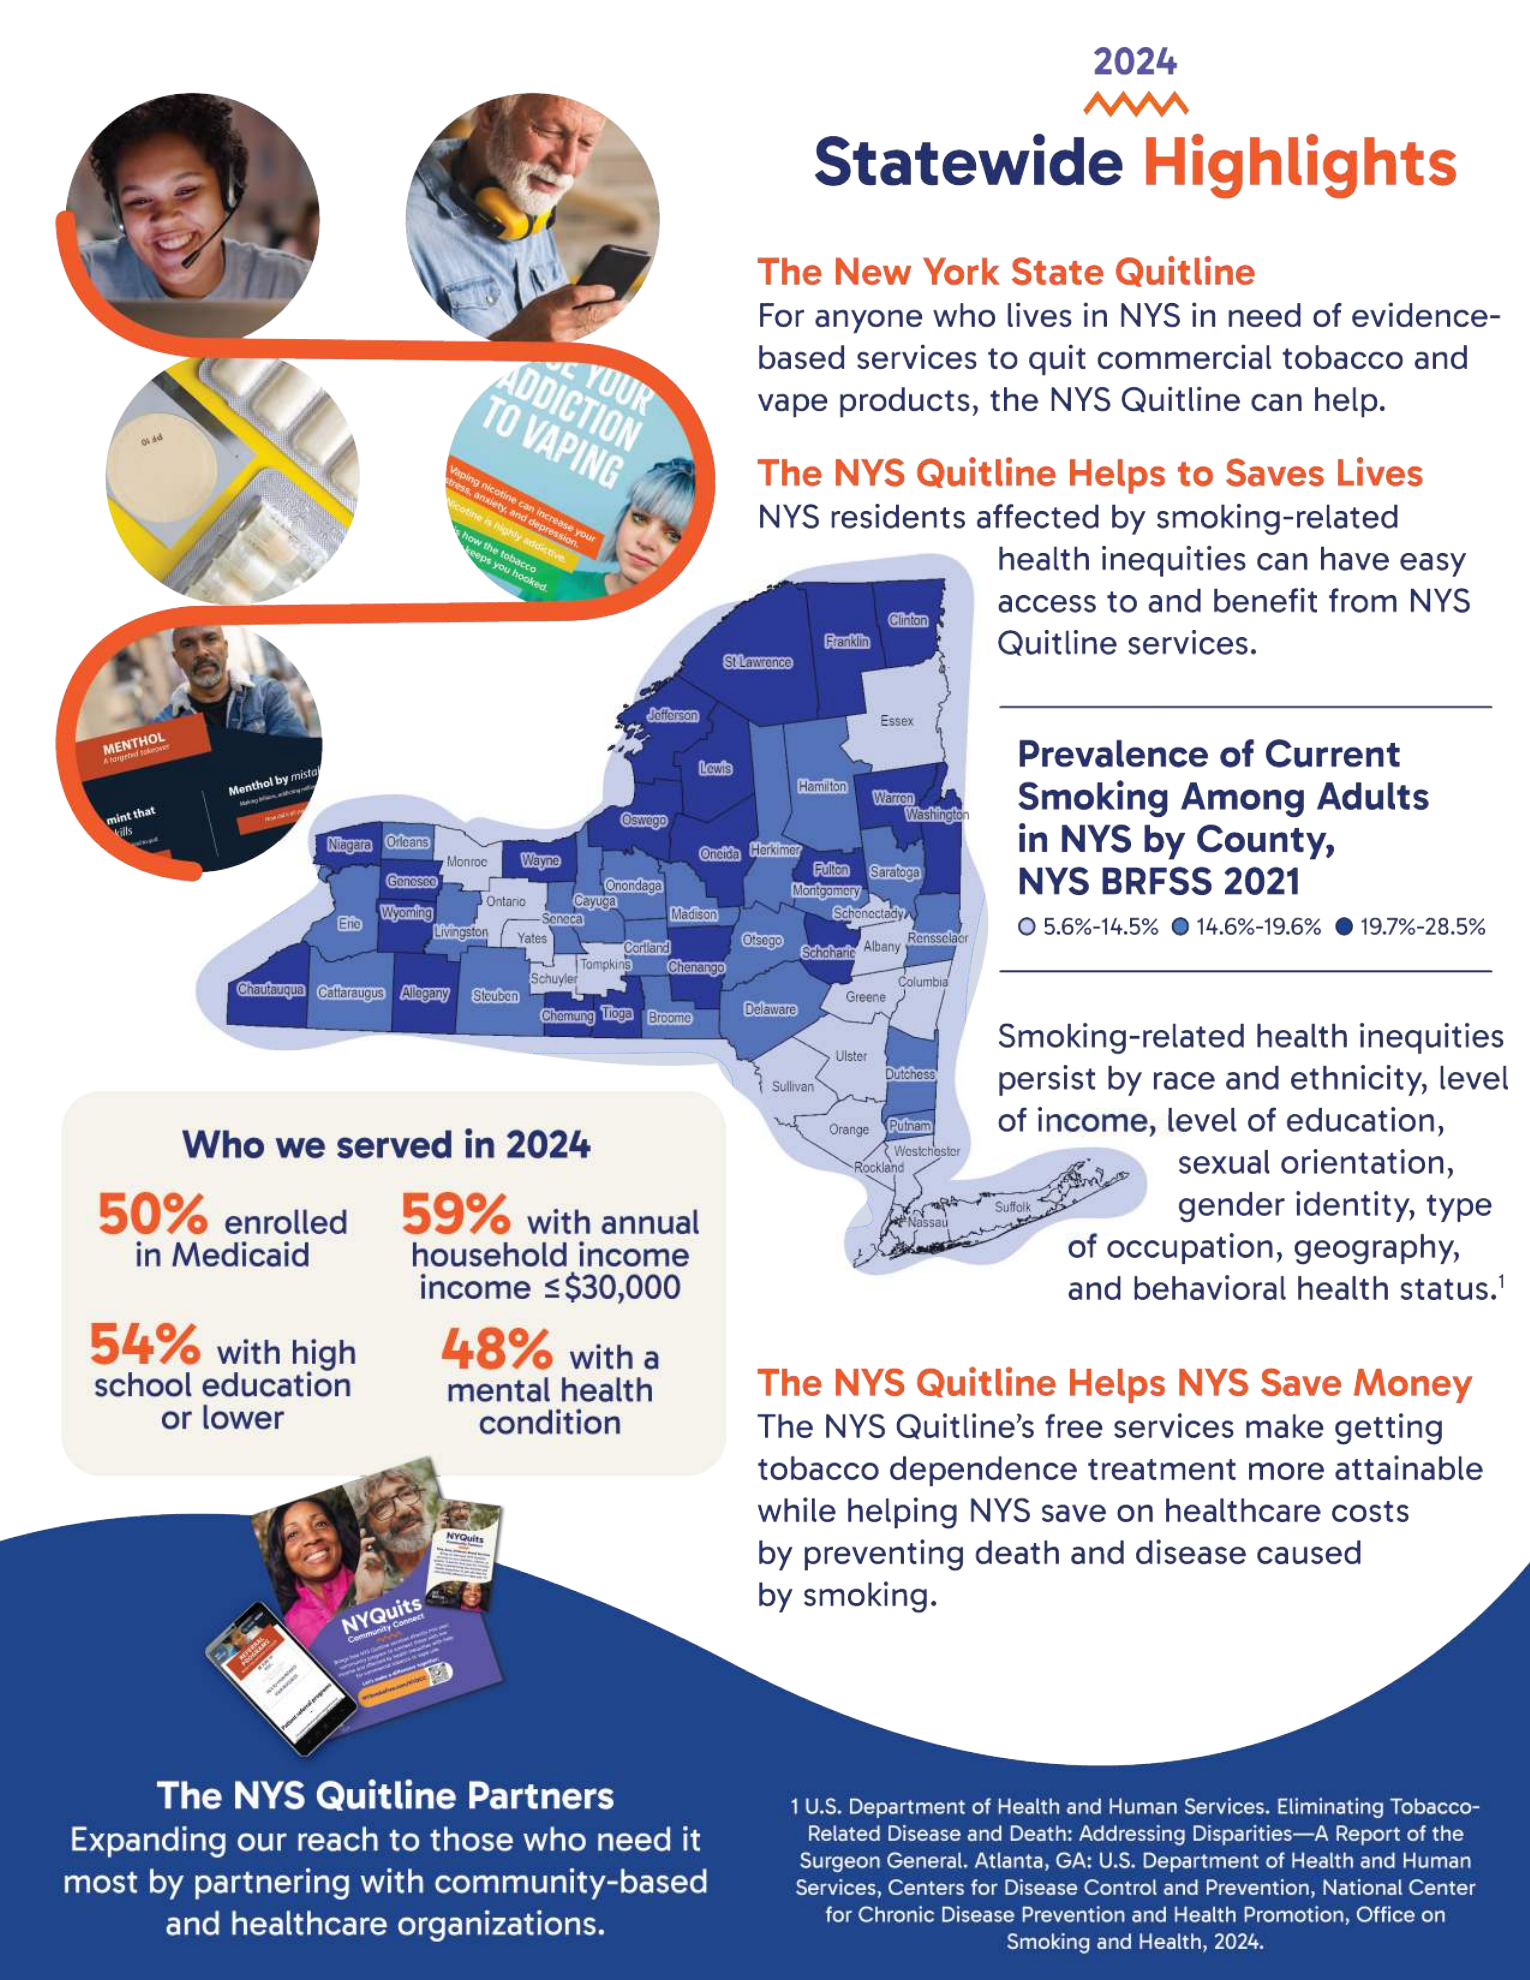
\includegraphics[width=1\linewidth,height=\textheight,keepaspectratio]{chapters/../media/figure-168-nys-smokefree-statewide-highlights.png}

}

\caption{\label{fig-nys-smokefree-statewide-highlights}2024 NYS Smokers
Quitline statewide highlights graphic}

\end{figure}%

\begin{tcolorbox}[enhanced jigsaw, opacitybacktitle=0.6, title=\textcolor{quarto-callout-note-color}{\faInfo}\hspace{0.5em}{Source}, coltitle=black, bottomrule=.15mm, leftrule=.75mm, colframe=quarto-callout-note-color-frame, colbacktitle=quarto-callout-note-color!10!white, rightrule=.15mm, breakable, bottomtitle=1mm, left=2mm, opacityback=0, titlerule=0mm, colback=white, arc=.35mm, toprule=.15mm, toptitle=1mm]

NYS Smokers' Quitline, 2024
https://www.nysmokefree.com/wp-content/uploads/2025/02/2024\_SustainabilityReport\_StatewideHighlights.pdf

\end{tcolorbox}

From 2016 to 2021, the percentage of adults who smoked cigarettes
decreased in almost every county in the M-H Region, with the exception
of Dutchess and Rockland Counties, NYS, and NYS excluding NYC. In 2021,
Dutchess County had the highest percentage of adults who smoked
cigarettes and Westchester County had the lowest percentage (17.4\% and
6.3\%, respectively). The Healthy People 2030 goal is to reduce
cigarette smoking among adults to 6.1\% (179).
Figure~\ref{fig-adult-currsmoke-percent}

\begin{figure}

\centering{

\begin{verbatim}
Unable to display output for mime type(s): text/html
\end{verbatim}

}

\caption{\label{fig-adult-currsmoke-percent}Percentage of Adults Who Are
Current Smokers, 2016, 2018, and 2021}

\end{figure}%

\begin{longtable}[]{@{}lllllllllll@{}}

\caption{\label{tbl-adult-currsmoke-percent}Percentage of Adults Who Are
Current Smokers, 2016, 2018, and 2021}

\tabularnewline

\caption{}\label{T_d02fe}\tabularnewline
\toprule\noalign{}
Year & Dutchess & Orange & Putnam & Rockland & Sullivan & Ulster &
Westchester & Mid-Hudson & NYS excl NYC & NYS \\
\midrule\noalign{}
\endfirsthead
\toprule\noalign{}
Year & Dutchess & Orange & Putnam & Rockland & Sullivan & Ulster &
Westchester & Mid-Hudson & NYS excl NYC & NYS \\
\midrule\noalign{}
\endhead
\bottomrule\noalign{}
\endlastfoot
2016 & 16.4 & 13.2 & 18.3 & 6.6 & 20.1 & 15.6 & 9.4 & 11.7 & 17.0 &
14.5 \\
2018 & 12.2 & 11.7 & 9.0 & 7.6 & 21.6 & 14.7 & 7.4 & 10.2 & 14.7 &
13.2 \\
2021 & 17.4 & 12.0 & 16.7 & 14.0 & 13.3 & 12.7 & 6.3 & 11.1 & 14.1 &
12.5 \\

\end{longtable}

\begin{tcolorbox}[enhanced jigsaw, opacitybacktitle=0.6, title=\textcolor{quarto-callout-note-color}{\faInfo}\hspace{0.5em}{Source}, coltitle=black, bottomrule=.15mm, leftrule=.75mm, colframe=quarto-callout-note-color-frame, colbacktitle=quarto-callout-note-color!10!white, rightrule=.15mm, breakable, bottomtitle=1mm, left=2mm, opacityback=0, titlerule=0mm, colback=white, arc=.35mm, toprule=.15mm, toptitle=1mm]

NYSDOH Behavioral Risk Factor Surveillance System, May 2025
https://www.health.ny.gov/statistics/brfss/expanded/

\end{tcolorbox}

\begin{tcolorbox}[enhanced jigsaw, opacitybacktitle=0.6, title=\textcolor{quarto-callout-note-color}{\faInfo}\hspace{0.5em}{Note}, coltitle=black, bottomrule=.15mm, leftrule=.75mm, colframe=quarto-callout-note-color-frame, colbacktitle=quarto-callout-note-color!10!white, rightrule=.15mm, breakable, bottomtitle=1mm, left=2mm, opacityback=0, titlerule=0mm, colback=white, arc=.35mm, toprule=.15mm, toptitle=1mm]

*: Percentage is unreliable due to large standard error. Note: The
percentage is age-adjusted. An adult is a person aged 18 years or older.
The Behavioral Risk Factor Surveillance System asks respondents, ``Have
you smoked at least 100 cigarettes in your entire life?'' and ``How long
has it been since you last smoked a cigarette, even one or two puffs?''
Based on responses to both questions, BRFSS defines ``current smoker''
as an adult over the age of 18 who has smoked at least 100 cigarettes in
their lifetime and currently smokes on at least some days.

\end{tcolorbox}

Although tobacco use appears to be decreasing over time, the use of
electronic nicotine delivery systems (ENDS), or vaping, has become
widely popular over the past few years. Electronic nicotine delivery
systems (electronic cigarettes or e-cigarettes, vaping pens, hookah
pens, etc.) were originally created to provide alternative products for
people trying to quit smoking cigarettes. Although use became a trend
among young adults, according to the NYSDOH, e-cigarette use among high
school youth appears to have peaked in 2018 at 27.4\% and declined to
18.7\% in 2022. Similarly, use of any tobacco product among high school
students, including ENDS, has decreased since 2018 from 30.6\% to 20.8\%
in 2022 and has reached the lowest youth smoking rate on record. (180)

For more information, please visit the CDC's Electronic Cigarette page
(181).

For more information on how to quit smoking, call 1-866-NY-QUITS or
visit https://nysmokefree.com/.

\subsection{Alcohol}\label{alcohol}

Excessive alcohol use has led to more than 170,000 deaths and about 4
million years of potential life lost each year in the U.S. from 2020 to
2021 (182). Binge drinking, defined as when women have four or more
drinks or men have five or more drinks on one occasion, is the most
common pattern of excessive alcohol use (183). Among adults in the
United States, 17\% binge drink (184).

Binge drinking decreased in almost all counties in the M-H Region from
2016 to 2021, with the exception of Rockland and Sullivan Counties.
Putnam County had the highest percentage of adults binge drinking in
2021 at 18.7\%, and Rockland County had the lowest percentage at 12.2\%
Figure~\ref{fig-adult-bingedrink-percent}.

\begin{figure}

\centering{

\begin{verbatim}
Unable to display output for mime type(s): text/html
\end{verbatim}

}

\caption{\label{fig-adult-bingedrink-percent}Percentage of Adults Binge
Drinking During the Past Month, 2016, 2018, and 2021}

\end{figure}%

\begin{longtable}[]{@{}lllllllllll@{}}

\caption{\label{tbl-adult-bingedrink-percent}Percentage of Adults Binge
Drinking During the Past Month, 2016, 2018, and 2021}

\tabularnewline

\caption{}\label{T_4f93e}\tabularnewline
\toprule\noalign{}
Year & Dutchess & Orange & Putnam & Rockland & Sullivan & Ulster &
Westchester & Mid-Hudson & NYS excl NYC & NYS \\
\midrule\noalign{}
\endfirsthead
\toprule\noalign{}
Year & Dutchess & Orange & Putnam & Rockland & Sullivan & Ulster &
Westchester & Mid-Hudson & NYS excl NYC & NYS \\
\midrule\noalign{}
\endhead
\bottomrule\noalign{}
\endlastfoot
2016 & 17.5 & 15.7 & 21.7 & 11.0 & 15.7 & 22.2 & 20.7 & 18.1 & 19.1 &
18.3 \\
2018 & 20.7 & 16.1 & 14.1 & 12.6 & 22.1 & 18.5 & 16.7 & 16.1 & 18.4 &
17.5 \\
2021 & 15.1 & 13.8 & 18.7 & 12.2 & 17.8 & 13.9 & 13.0 & 13.1 & 16.1 &
16.0 \\

\end{longtable}

\begin{tcolorbox}[enhanced jigsaw, opacitybacktitle=0.6, title=\textcolor{quarto-callout-note-color}{\faInfo}\hspace{0.5em}{Source}, coltitle=black, bottomrule=.15mm, leftrule=.75mm, colframe=quarto-callout-note-color-frame, colbacktitle=quarto-callout-note-color!10!white, rightrule=.15mm, breakable, bottomtitle=1mm, left=2mm, opacityback=0, titlerule=0mm, colback=white, arc=.35mm, toprule=.15mm, toptitle=1mm]

NYSDOH Behavioral Risk Factor Surveillance System, May 2025
https://www.health.ny.gov/statistics/brfss/expanded/

\end{tcolorbox}

\begin{tcolorbox}[enhanced jigsaw, opacitybacktitle=0.6, title=\textcolor{quarto-callout-note-color}{\faInfo}\hspace{0.5em}{Note}, coltitle=black, bottomrule=.15mm, leftrule=.75mm, colframe=quarto-callout-note-color-frame, colbacktitle=quarto-callout-note-color!10!white, rightrule=.15mm, breakable, bottomtitle=1mm, left=2mm, opacityback=0, titlerule=0mm, colback=white, arc=.35mm, toprule=.15mm, toptitle=1mm]

Note: The percentage is age-adjusted. An adult is a person aged 18 years
or older. The Behavioral Risk Factor Surveillance System asks
respondents, ``Considering all types of alcoholic beverages, how many
times during the past 30 days did you have (for men) 5 or more drinks on
an occasion or (for women) 4 or more drinks on an occasion?'' Based on
the responses to this question ``binge drinking'' is defined as
consuming 4 or more drinks for women and 5 or more drinks for men on a
single occasion.

\end{tcolorbox}

Binge drinking can lead to many different health and social problems,
including unintentional motor vehicle accidents. In 2023, 30\% of
traffic-related deaths in the U.S. were due to alcohol-impaired driving
(185). For regional data regarding alcohol-related motor vehicle
injuries and deaths, refer to the Motor Vehicle Accidents section.

\subsection{Opioid Use}\label{opioid-use}

Opioids are a class of drugs that include illicit drugs such as heroin,
synthetic opioids such as fentanyl, and prescription pain relievers such
as oxycodone, hydrocodone, and morphine. According to the CDC, in 2023
about 76\% of drug overdoses involved an opioid, and deaths involving
multiple drugs also increased (186). The financial costs of management,
treatment, and lost productivity due to misuse of illicit drugs,
prescription drugs, and alcohol were estimated at \$442 billion in 2012
(173).

From 2019 to 2020, ED visit rates for overdoses involving any opioid
increased in almost all seven counties in the M-H Region except
Westchester. Since 2020, rates have fallen or remained relatively stable
in all seven counties in the M-H Region, as well as in NYS and NYS
excluding NYC Figure~\ref{fig-ed-visit-opioid-aar}.

\begin{figure}

\centering{

\begin{verbatim}
Unable to display output for mime type(s): text/html
\end{verbatim}

}

\caption{\label{fig-ed-visit-opioid-aar}All Emergency Department Visits
Involving Any Opioid Overdose, Age-Adjusted Rate per 100,000 Population,
2019--2022}

\end{figure}%

\begin{longtable}[]{@{}lllllllllll@{}}

\caption{\label{tbl-ed-visit-opioid-aar}All Emergency Department Visits
Involving Any Opioid Overdose, Age-Adjusted Rate per 100,000 Population,
2019--2022}

\tabularnewline

\caption{}\label{T_ed7dc}\tabularnewline
\toprule\noalign{}
Year & Dutchess & Orange & Putnam & Rockland & Sullivan & Ulster &
Westchester & Mid-Hudson & NYS excl NYC & NYS \\
\midrule\noalign{}
\endfirsthead
\toprule\noalign{}
Year & Dutchess & Orange & Putnam & Rockland & Sullivan & Ulster &
Westchester & Mid-Hudson & NYS excl NYC & NYS \\
\midrule\noalign{}
\endhead
\bottomrule\noalign{}
\endlastfoot
2019 & 98.8 & 62.8 & 51.6 & 29.1 & 84.8 & 94.1 & 35.2 & 53.7 & 66.7 &
54.1 \\
2020 & 88.9 & 82.7 & 55.7 & 38.7 & 154.3 & 127.2 & 34.1 & 61.8 & 74.3 &
61.0 \\
2021 & 83.9 & 64.0 & 60.9 & 36.1 & 136.9 & 113.9 & 39.4 & 58.8 & 73.1 &
67.2 \\
2022 & 77.9 & 64.5 & 40.1 & 28.4 & 123.9 & 80.4 & 34.8 & 51.1 & 64.8 &
67.1 \\

\end{longtable}

\begin{tcolorbox}[enhanced jigsaw, opacitybacktitle=0.6, title=\textcolor{quarto-callout-note-color}{\faInfo}\hspace{0.5em}{Source}, coltitle=black, bottomrule=.15mm, leftrule=.75mm, colframe=quarto-callout-note-color-frame, colbacktitle=quarto-callout-note-color!10!white, rightrule=.15mm, breakable, bottomtitle=1mm, left=2mm, opacityback=0, titlerule=0mm, colback=white, arc=.35mm, toprule=.15mm, toptitle=1mm]

NYS Opioid Data Dashboard, May 2025 sourced from NY Statewide Planning
and Research Cooperative System
https://apps.health.ny.gov/public/tabvis/PHIG\_Public/opioid/

\end{tcolorbox}

\begin{tcolorbox}[enhanced jigsaw, opacitybacktitle=0.6, title=\textcolor{quarto-callout-note-color}{\faInfo}\hspace{0.5em}{Note}, coltitle=black, bottomrule=.15mm, leftrule=.75mm, colframe=quarto-callout-note-color-frame, colbacktitle=quarto-callout-note-color!10!white, rightrule=.15mm, breakable, bottomtitle=1mm, left=2mm, opacityback=0, titlerule=0mm, colback=white, arc=.35mm, toprule=.15mm, toptitle=1mm]

Note: Includes outpatient and admitted patient visits to the emergency
department involving any opioid poisoning as the principal diagnosis or
first-listed cause of injury.

\end{tcolorbox}

Hospital discharges involving any opioid overdose have generally
remained stable over time, with the exception of Sullivan County, which
saw a large rate increase in 2020 before rates began to decrease
Figure~\ref{fig-hospital-dc-opioid-aar}.

\begin{figure}

\centering{

\begin{verbatim}
Unable to display output for mime type(s): text/html
\end{verbatim}

}

\caption{\label{fig-hospital-dc-opioid-aar}Hospital Discharges Involving
Any Opioid Overdose, Age-Adjusted Rate per 100,000 Population,
2019--2022}

\end{figure}%

\begin{longtable}[]{@{}lllllllllll@{}}

\caption{\label{tbl-hospital-dc-opioid-aar}Hospital Discharges Involving
Any Opioid Overdose, Age-Adjusted Rate per 100,000 Population,
2019--2022}

\tabularnewline

\caption{}\label{T_2632f}\tabularnewline
\toprule\noalign{}
Year & Dutchess & Orange & Putnam & Rockland & Sullivan & Ulster &
Westchester & Mid-Hudson & NYS excl NYC & NYS \\
\midrule\noalign{}
\endfirsthead
\toprule\noalign{}
Year & Dutchess & Orange & Putnam & Rockland & Sullivan & Ulster &
Westchester & Mid-Hudson & NYS excl NYC & NYS \\
\midrule\noalign{}
\endhead
\bottomrule\noalign{}
\endlastfoot
2019 & 19.1 & 13.8 & 9.3 & 8.8 & 16.8 & 18.4 & 10.4 & 12.6 & 13.4 &
13.6 \\
2020 & 17.3 & 15.0 & 13.7 & 10.0 & 28.1 & 16.0 & 10.1 & 13.0 & 14.3 &
14.9 \\
2021 & 17.0 & 11.5 & 9.5* & 8.5 & 22.0 & 19.2 & 11.9 & 12.9 & 13.7 &
15.2 \\
2022 & 13.9 & 13.0 & 9.9 & 9.6 & 16.6 & 14.7 & 8.0 & 10.7 & 12.1 &
15.8 \\

\end{longtable}

\begin{tcolorbox}[enhanced jigsaw, opacitybacktitle=0.6, title=\textcolor{quarto-callout-note-color}{\faInfo}\hspace{0.5em}{Source}, coltitle=black, bottomrule=.15mm, leftrule=.75mm, colframe=quarto-callout-note-color-frame, colbacktitle=quarto-callout-note-color!10!white, rightrule=.15mm, breakable, bottomtitle=1mm, left=2mm, opacityback=0, titlerule=0mm, colback=white, arc=.35mm, toprule=.15mm, toptitle=1mm]

NYS Opioid Data Dashboard, May 2025 sourced from NY Statewide Planning
and Research Cooperative System
https://apps.health.ny.gov/public/tabvis/PHIG\_Public/opioid/

\end{tcolorbox}

\begin{tcolorbox}[enhanced jigsaw, opacitybacktitle=0.6, title=\textcolor{quarto-callout-note-color}{\faInfo}\hspace{0.5em}{Note}, coltitle=black, bottomrule=.15mm, leftrule=.75mm, colframe=quarto-callout-note-color-frame, colbacktitle=quarto-callout-note-color!10!white, rightrule=.15mm, breakable, bottomtitle=1mm, left=2mm, opacityback=0, titlerule=0mm, colback=white, arc=.35mm, toprule=.15mm, toptitle=1mm]

*: The rate is unstable. Note: Y-axis does not begin at zero in order to
clearly display trend lines. Includes hospital discharges involving any
opioid poisoning, principal diagnosis or first-listed cause of injury.

\end{tcolorbox}

Substance use treatment is intended to help people address problems
associated with their use of alcohol or drugs, including related medical
problems. Data on who actually seeks help can indicate whether
interventions are effectively reaching those in need. In 2019, about
21.6 million people needed substance use treatment, but only 2.6 million
received it. Despite increased awareness of the opioid epidemic, as well
as laws and regulations that expanded treatment coverage, there has been
no consistent upward trend in people seeking and accessing treatment
(187). This flattened trend is evident in the M-H Region, where in most
counties the number of individuals enrolled in OASAS-certified substance
use disorder programs has remained relatively level
Figure~\ref{fig-treat-prog-opioid-crude}.

\begin{figure}

\centering{

\begin{verbatim}
Unable to display output for mime type(s): text/html
\end{verbatim}

}

\caption{\label{fig-treat-prog-opioid-crude}Individuals Enrolled in
Treatment Programs Reporting Any Opioid as a Primary Substance, Crude
Rate per 100,000 Population, 2020--2023}

\end{figure}%

\begin{longtable}[]{@{}llllllll@{}}

\caption{\label{tbl-treat-prog-opioid-crude}Individuals Enrolled in
Treatment Programs Reporting Any Opioid as a Primary Substance, Crude
Rate per 100,000 Population, 2020--2023}

\tabularnewline

\caption{}\label{T_4b1cf}\tabularnewline
\toprule\noalign{}
Year & Dutchess & Orange & Putnam & Rockland & Sullivan & Ulster &
Westchester \\
\midrule\noalign{}
\endfirsthead
\toprule\noalign{}
Year & Dutchess & Orange & Putnam & Rockland & Sullivan & Ulster &
Westchester \\
\midrule\noalign{}
\endhead
\bottomrule\noalign{}
\endlastfoot
2020 & 459.9 & 405.4 & 248.8 & 188.9 & 693.2 & 487.8 & 255.1 \\
2021 & 475.0 & 393.7 & 252.1 & 197.9 & 710.7 & 531.2 & 251.9 \\
2022 & 460.8 & 366.9 & 250.1 & 188.2 & 777.4 & 516.0 & 244.4 \\
2023 & 447.6 & 333.5 & 224.5 & 190.9 & 778.3 & 496.4 & 233.2 \\

\end{longtable}

\begin{tcolorbox}[enhanced jigsaw, opacitybacktitle=0.6, title=\textcolor{quarto-callout-note-color}{\faInfo}\hspace{0.5em}{Source}, coltitle=black, bottomrule=.15mm, leftrule=.75mm, colframe=quarto-callout-note-color-frame, colbacktitle=quarto-callout-note-color!10!white, rightrule=.15mm, breakable, bottomtitle=1mm, left=2mm, opacityback=0, titlerule=0mm, colback=white, arc=.35mm, toprule=.15mm, toptitle=1mm]

Data request from NYS Office of Addiction Services and Supports Client
Data System, May 2025

\end{tcolorbox}

\begin{tcolorbox}[enhanced jigsaw, opacitybacktitle=0.6, title=\textcolor{quarto-callout-note-color}{\faInfo}\hspace{0.5em}{Note}, coltitle=black, bottomrule=.15mm, leftrule=.75mm, colframe=quarto-callout-note-color-frame, colbacktitle=quarto-callout-note-color!10!white, rightrule=.15mm, breakable, bottomtitle=1mm, left=2mm, opacityback=0, titlerule=0mm, colback=white, arc=.35mm, toprule=.15mm, toptitle=1mm]

Note: This indicator includes people who were admitted to an
OASAS-certified substance use disorder treatment program. A person is
counted once if they were in treatment (received one or more services)
during the calendar year. A unique person may receive multiple services
or be in treatment for many years and, therefore, may be counted
uniquely across one or more calendar years. Totals cannot be summed
across years/rows because they are not mutually exclusive. The most
recent data collected for the year of enrollment was used to determine
the person's county of residence during the reported year. Any opioid
use includes heroin use.

\end{tcolorbox}

From 2019 to 2022, the rate of overdose deaths involving any opioid
steadily increased across most counties in the M-H Region, as well as in
NYS and NYS excluding NYC. In 2022, the highest rate was in Sullivan
County and the lowest rate was in Rockland County (61.5 and 12.9 per
100,000 population, respectively) Figure~\ref{fig-od-anyopioid-crude}.

\begin{figure}

\centering{

\begin{verbatim}
Unable to display output for mime type(s): text/html
\end{verbatim}

}

\caption{\label{fig-od-anyopioid-crude}Overdose Deaths Involving Any
Opioid, Crude Rate per 100,000 Population, 2019--2022}

\end{figure}%

\begin{longtable}[]{@{}lllllllllll@{}}

\caption{\label{tbl-od-anyopioid-crude}Overdose Deaths Involving Any
Opioid, Crude Rate per 100,000 Population, 2019--2022}

\tabularnewline

\caption{}\label{T_64b02}\tabularnewline
\toprule\noalign{}
Year & Dutchess & Orange & Putnam & Rockland & Sullivan & Ulster &
Westchester & Mid-Hudson & NYS excl NYC & NYS \\
\midrule\noalign{}
\endfirsthead
\toprule\noalign{}
Year & Dutchess & Orange & Putnam & Rockland & Sullivan & Ulster &
Westchester & Mid-Hudson & NYS excl NYC & NYS \\
\midrule\noalign{}
\endhead
\bottomrule\noalign{}
\endlastfoot
2019 & 22.1 & 20.7 & 12.1 & 14.1 & 39.8 & 17.9 & 9.4 & 15.3 & 16.1 &
15.1 \\
2020 & 35.7 & 26.9 & 18.2 & 12.9 & 63.7 & 31.4 & 13.8 & 21.8 & 22.7 &
21.5 \\
2021 & 29.1 & 33.8 & 20.4 & 19.1 & 46.4 & 25.6 & 15.0 & 22.6 & 25.2 &
25.1 \\
2022 & 39.3 & 30.5 & 22.4 & 12.9 & 61.5 & 35.7 & 15.4 & 24.0 & 26.3 &
27.4 \\

\end{longtable}

\begin{tcolorbox}[enhanced jigsaw, opacitybacktitle=0.6, title=\textcolor{quarto-callout-note-color}{\faInfo}\hspace{0.5em}{Source}, coltitle=black, bottomrule=.15mm, leftrule=.75mm, colframe=quarto-callout-note-color-frame, colbacktitle=quarto-callout-note-color!10!white, rightrule=.15mm, breakable, bottomtitle=1mm, left=2mm, opacityback=0, titlerule=0mm, colback=white, arc=.35mm, toprule=.15mm, toptitle=1mm]

NYS Opioid Data Dashboard, May 2025 sourced from Vital Statistics of NYS
https://apps.health.ny.gov/public/tabvis/PHIG\_Public/opioid/

\end{tcolorbox}

\begin{tcolorbox}[enhanced jigsaw, opacitybacktitle=0.6, title=\textcolor{quarto-callout-note-color}{\faInfo}\hspace{0.5em}{Note}, coltitle=black, bottomrule=.15mm, leftrule=.75mm, colframe=quarto-callout-note-color-frame, colbacktitle=quarto-callout-note-color!10!white, rightrule=.15mm, breakable, bottomtitle=1mm, left=2mm, opacityback=0, titlerule=0mm, colback=white, arc=.35mm, toprule=.15mm, toptitle=1mm]

*: The rate is unstable. Note: Includes poisoning deaths involving any
opioid, all manners, using all causes of death.

\end{tcolorbox}

Figure~\ref{fig-od-multiple-opioid-aar} shows the rate of overdose
deaths in 2022 stratified by the type of opioid used. The highest rate
of overdose deaths in all counties was caused by opioid pain relievers.
Synthetic opioids other than methadone were a close second.

\begin{figure}

\centering{

\begin{verbatim}
Unable to display output for mime type(s): text/html
\end{verbatim}

}

\caption{\label{fig-od-multiple-opioid-aar}Overdose Deaths Involving
Opioid Pain Relievers, Heroin, and Synthetic Opioids Other than
Methadone, Age-Adjusted Rate per 100,000 Population, 2022}

\end{figure}%

\begin{longtable}[]{@{}lllllllllll@{}}

\caption{\label{tbl-od-multiple-opioid-aar}Overdose Deaths Involving
Opioid Pain Relievers, Heroin, and Synthetic Opioids Other than
Methadone, Age-Adjusted Rate per 100,000 Population, 2022}

\tabularnewline

\caption{}\label{T_5cc8e}\tabularnewline
\toprule\noalign{}
& Dutchess & Orange & Putnam & Rockland & Sullivan & Ulster &
Westchester & Mid-Hudson & NYS excl NYC & NYS \\
\midrule\noalign{}
\endfirsthead
\toprule\noalign{}
& Dutchess & Orange & Putnam & Rockland & Sullivan & Ulster &
Westchester & Mid-Hudson & NYS excl NYC & NYS \\
\midrule\noalign{}
\endhead
\bottomrule\noalign{}
\endlastfoot
Opioid Pain Relievers & 39.6 & 31.1 & 19.8 & 14.2 & 62.5 & 34.7 & 15.5 &
24.1 & 27.3 & 26.3 \\
Heroin & 3.5 & 5.9 & 2.2 & 2.2 & 10.1 & 2.8 & 2.0 & 3.1 & 2.0 & 4.2 \\
Synthetic Opioids Other Than Methadone & 37.2 & 28.0 & 18.0 & 12.6 &
58.1 & 32.6 & 13.8 & 22.0 & 25.4 & 24.8 \\

\end{longtable}

\begin{tcolorbox}[enhanced jigsaw, opacitybacktitle=0.6, title=\textcolor{quarto-callout-note-color}{\faInfo}\hspace{0.5em}{Note}, coltitle=black, bottomrule=.15mm, leftrule=.75mm, colframe=quarto-callout-note-color-frame, colbacktitle=quarto-callout-note-color!10!white, rightrule=.15mm, breakable, bottomtitle=1mm, left=2mm, opacityback=0, titlerule=0mm, colback=white, arc=.35mm, toprule=.15mm, toptitle=1mm]

*: The rate is unstable. Note: Includes poisoning deaths involving any
opioid pain relievers (including illicitly produced opioids such as
fentanyl), heroin, and synthetic opioids other than methadone, all
manners, using all causes of death.

\end{tcolorbox}

When overdose deaths are stratified by age, the rate of overdose death
was higher in most counties among adults aged 45 to 64 years compared
with those aged 18 to 44 years across all three types of overdose deaths
(any opioid, heroin, and opioid pain relievers)
Figure~\ref{fig-18to64-anyop-od-crude}. This shows a shift from previous
years, when overdose deaths were predominantly among adults aged 18 to
44 years. Sullivan County had the highest overdose death rates among
adults aged 18 to 44 years caused by all three types (99.9, 11.5, and
99.9 per 100,000 population, respectively), as well as among adults aged
45 to 64 years (89.3, 23.5, and 89.3 per 100,000 population,
respectively).

\begin{figure}

\centering{

\begin{verbatim}
Unable to display output for mime type(s): text/html
\end{verbatim}

}

\caption{\label{fig-18to64-anyop-od-crude}Overdose Deaths among Adults
Involving Any Opioid, Crude Rate per 100,000 Population, 2022}

\end{figure}%

\begin{longtable}[]{@{}lllllllllll@{}}

\caption{\label{tbl-18to64-anyop-od-crude}Overdose Deaths among Adults
Involving Any Opioid, Crude Rate per 100,000 Population, 2022}

\tabularnewline

\caption{}\label{T_e1c86}\tabularnewline
\toprule\noalign{}
Age Group & Dutchess & Orange & Putnam & Rockland & Sullivan & Ulster &
Westchester & Mid-Hudson & NYS excl NYC & NYS \\
\midrule\noalign{}
\endfirsthead
\toprule\noalign{}
Age Group & Dutchess & Orange & Putnam & Rockland & Sullivan & Ulster &
Westchester & Mid-Hudson & NYS excl NYC & NYS \\
\midrule\noalign{}
\endhead
\bottomrule\noalign{}
\endlastfoot
18--44 years & 63.1 & 42.0 & 31.9 & 21.2 & 99.9 & 51.6 & 24.4 & 36.9 &
42.4 & 36.7 \\
45--64 years & 55.4 & 51.0 & 34.4 & 24.6 & 89.3 & 53.6 & 22.7 & 37.0 &
39.2 & 46.9 \\

\end{longtable}

\begin{tcolorbox}[enhanced jigsaw, opacitybacktitle=0.6, title=\textcolor{quarto-callout-note-color}{\faInfo}\hspace{0.5em}{Source}, coltitle=black, bottomrule=.15mm, leftrule=.75mm, colframe=quarto-callout-note-color-frame, colbacktitle=quarto-callout-note-color!10!white, rightrule=.15mm, breakable, bottomtitle=1mm, left=2mm, opacityback=0, titlerule=0mm, colback=white, arc=.35mm, toprule=.15mm, toptitle=1mm]

Source: NYS Opioid Data Dashboard, May 2025 sourced from Vital
Statistics of NYS
https://apps.health.ny.gov/public/tabvis/PHIG\_Public/opioid/

\end{tcolorbox}

\begin{tcolorbox}[enhanced jigsaw, opacitybacktitle=0.6, title=\textcolor{quarto-callout-note-color}{\faInfo}\hspace{0.5em}{Note}, coltitle=black, bottomrule=.15mm, leftrule=.75mm, colframe=quarto-callout-note-color-frame, colbacktitle=quarto-callout-note-color!10!white, rightrule=.15mm, breakable, bottomtitle=1mm, left=2mm, opacityback=0, titlerule=0mm, colback=white, arc=.35mm, toprule=.15mm, toptitle=1mm]

Note: This includes adults aged 18--64 years old. Includes all poisoning
deaths involving opioids, all manners, using all causes of death.

\end{tcolorbox}

\begin{figure}

\centering{

\begin{verbatim}
Unable to display output for mime type(s): text/html
\end{verbatim}

}

\caption{\label{fig-18to64-heroin-od-crude}Overdose Deaths among Adults
Involving Heroin, Crude Rate per 100,000 Population, 2022}

\end{figure}%

\begin{longtable}[]{@{}lllllllllll@{}}

\caption{\label{tbl-18to64-heroin-od-crude}Overdose Deaths among Adults
Involving Heroin, Crude Rate per 100,000 Population, 2022}

\tabularnewline

\caption{}\label{T_7bb31}\tabularnewline
\toprule\noalign{}
Age Group & Dutchess & Orange & Putnam & Rockland & Sullivan & Ulster &
Westchester & Mid-Hudson & NYS excl NYC & NYS \\
\midrule\noalign{}
\endfirsthead
\toprule\noalign{}
Age Group & Dutchess & Orange & Putnam & Rockland & Sullivan & Ulster &
Westchester & Mid-Hudson & NYS excl NYC & NYS \\
\midrule\noalign{}
\endhead
\bottomrule\noalign{}
\endlastfoot
18--44 years & 5.8* & 6.4* & 3.2* & 0.9* & 11.5* & 4.8* & 3.7 & 4.4 &
3.1 & 4.5 \\
45--64 years & 6.0* & 10.8 & 3.4* & 7.8* & 23.5* & 4.0* & 2.6* & 5.8 &
2.9 & 9.1 \\

\end{longtable}

\begin{tcolorbox}[enhanced jigsaw, opacitybacktitle=0.6, title=\textcolor{quarto-callout-note-color}{\faInfo}\hspace{0.5em}{Source}, coltitle=black, bottomrule=.15mm, leftrule=.75mm, colframe=quarto-callout-note-color-frame, colbacktitle=quarto-callout-note-color!10!white, rightrule=.15mm, breakable, bottomtitle=1mm, left=2mm, opacityback=0, titlerule=0mm, colback=white, arc=.35mm, toprule=.15mm, toptitle=1mm]

Source: NYS Opioid Data Dashboard, May 2025 sourced from Vital
Statistics of NYS
https://apps.health.ny.gov/public/tabvis/PHIG\_Public/opioid/

\end{tcolorbox}

\begin{tcolorbox}[enhanced jigsaw, opacitybacktitle=0.6, title=\textcolor{quarto-callout-note-color}{\faInfo}\hspace{0.5em}{Note}, coltitle=black, bottomrule=.15mm, leftrule=.75mm, colframe=quarto-callout-note-color-frame, colbacktitle=quarto-callout-note-color!10!white, rightrule=.15mm, breakable, bottomtitle=1mm, left=2mm, opacityback=0, titlerule=0mm, colback=white, arc=.35mm, toprule=.15mm, toptitle=1mm]

*: The rate is unstable. Note: This includes adults aged 18--64 years
old. Poisoning deaths involving heroin, all manners, using all causes of
death.

\end{tcolorbox}

\begin{figure}

\centering{

\begin{verbatim}
Unable to display output for mime type(s): text/html
\end{verbatim}

}

\caption{\label{fig-18to64-opioid-pain-crude}Overdose Deaths among
Adults Involving Opioid Pain Relievers, Crude Rate per 100,000
Population, 2022}

\end{figure}%

\begin{longtable}[]{@{}lllllllllll@{}}

\caption{\label{tbl-18to64-opioid-pain-crude}Overdose Deaths among
Adults Involving Opioid Pain Relievers, Crude Rate per 100,000
Population, 2022}

\tabularnewline

\caption{}\label{T_7eb2c}\tabularnewline
\toprule\noalign{}
Age Group & Dutchess & Orange & Putnam & Rockland & Sullivan & Ulster &
Westchester & Mid-Hudson & NYS excl NYC & NYS \\
\midrule\noalign{}
\endfirsthead
\toprule\noalign{}
Age Group & Dutchess & Orange & Putnam & Rockland & Sullivan & Ulster &
Westchester & Mid-Hudson & NYS excl NYC & NYS \\
\midrule\noalign{}
\endhead
\bottomrule\noalign{}
\endlastfoot
18--44 years & 63.1 & 42.0 & 28.7* & 21.2 & 99.9 & 51.6 & 24.4 & 36.8 &
41.9 & 36.1 \\
45--64 years & 55.4 & 50.0 & 34.4 & 24.6 & 89.3 & 51.6 & 22.4 & 36.5 &
38.8 & 46.3 \\

\end{longtable}

\begin{tcolorbox}[enhanced jigsaw, opacitybacktitle=0.6, title=\textcolor{quarto-callout-note-color}{\faInfo}\hspace{0.5em}{Source}, coltitle=black, bottomrule=.15mm, leftrule=.75mm, colframe=quarto-callout-note-color-frame, colbacktitle=quarto-callout-note-color!10!white, rightrule=.15mm, breakable, bottomtitle=1mm, left=2mm, opacityback=0, titlerule=0mm, colback=white, arc=.35mm, toprule=.15mm, toptitle=1mm]

NYS Opioid Data Dashboard, May 2025 sourced from Vital Statistics of NYS
https://apps.health.ny.gov/public/tabvis/PHIG\_Public/opioid/

\end{tcolorbox}

\begin{tcolorbox}[enhanced jigsaw, opacitybacktitle=0.6, title=\textcolor{quarto-callout-note-color}{\faInfo}\hspace{0.5em}{Note}, coltitle=black, bottomrule=.15mm, leftrule=.75mm, colframe=quarto-callout-note-color-frame, colbacktitle=quarto-callout-note-color!10!white, rightrule=.15mm, breakable, bottomtitle=1mm, left=2mm, opacityback=0, titlerule=0mm, colback=white, arc=.35mm, toprule=.15mm, toptitle=1mm]

*: The rate is unstable. Note: This includes adults aged 18--64 years
old. Includes poisoning deaths involving opioid pain relievers
(including illicitly produced opioids such as fentanyl), all manners,
using all causes of death.

\end{tcolorbox}

There are many efforts being made at the federal, state, and local
levels to combat the opioid epidemic. Methods include improving opioid
prescribing practices; increasing education, training, and distribution
of naloxone (an overdose reversal drug); and increasing access to
medication-assisted treatment (188).

From 2020 to 2023, prescription rates for opioid analgesics (pain
relievers) decreased across each county in the M-H Region, as well as in
NYS and NYS excluding NYC. In 2023, Sullivan County had the highest
opioid analgesic prescription rate and Westchester County had the lowest
rate (352.7 and 162.9 per 1,000 population, respectively)
Figure~\ref{fig-opioid-analgesic-rx-aar}.

\begin{figure}

\centering{

\begin{verbatim}
Unable to display output for mime type(s): text/html
\end{verbatim}

}

\caption{\label{fig-opioid-analgesic-rx-aar}Opioid Analgesics
Prescriptions, Age-Adjusted Rate per 1,000 Population, 2020--2023}

\end{figure}%

\begin{longtable}[]{@{}lllllllllll@{}}

\caption{\label{tbl-opioid-analgesic-rx-aar}Opioid Analgesics
Prescriptions, Age-Adjusted Rate per 1,000 Population, 2020--2023}

\tabularnewline

\caption{}\label{T_a8abb}\tabularnewline
\toprule\noalign{}
Year & Dutchess & Orange & Putnam & Rockland & Sullivan & Ulster &
Westchester & Mid-Hudson & NYS excl NYC & NYS \\
\midrule\noalign{}
\endfirsthead
\toprule\noalign{}
Year & Dutchess & Orange & Putnam & Rockland & Sullivan & Ulster &
Westchester & Mid-Hudson & NYS excl NYC & NYS \\
\midrule\noalign{}
\endhead
\bottomrule\noalign{}
\endlastfoot
2020 & 348.0 & 321.2 & 300.1 & 225.1 & 502.0 & 436.9 & 202.3 & 275.9 &
342.4 & 270.6 \\
2021 & 319.0 & 292.5 & 288.3 & 211.3 & 432.6 & 398.9 & 187.9 & 253.7 &
321.2 & 254.1 \\
2022 & 296.2 & 269.6 & 261.7 & 193.7 & 398.5 & 364.7 & 173.3 & 233.8 &
300.2 & 238.1 \\
2023 & 270.7 & 250.5 & 239.3 & 179.4 & 352.7 & 333.4 & 162.9 & 216.3 &
283.8 & 225.6 \\

\end{longtable}

\begin{tcolorbox}[enhanced jigsaw, opacitybacktitle=0.6, title=\textcolor{quarto-callout-note-color}{\faInfo}\hspace{0.5em}{Source}, coltitle=black, bottomrule=.15mm, leftrule=.75mm, colframe=quarto-callout-note-color-frame, colbacktitle=quarto-callout-note-color!10!white, rightrule=.15mm, breakable, bottomtitle=1mm, left=2mm, opacityback=0, titlerule=0mm, colback=white, arc=.35mm, toprule=.15mm, toptitle=1mm]

NYS Opioid Data Dashboard, May 2025 sourced from Vital Statistics of NYS
https://apps.health.ny.gov/public/tabvis/PHIG\_Public/opioid/

\end{tcolorbox}

\begin{tcolorbox}[enhanced jigsaw, opacitybacktitle=0.6, title=\textcolor{quarto-callout-note-color}{\faInfo}\hspace{0.5em}{Note}, coltitle=black, bottomrule=.15mm, leftrule=.75mm, colframe=quarto-callout-note-color-frame, colbacktitle=quarto-callout-note-color!10!white, rightrule=.15mm, breakable, bottomtitle=1mm, left=2mm, opacityback=0, titlerule=0mm, colback=white, arc=.35mm, toprule=.15mm, toptitle=1mm]

Note: Includes Schedule II (Drugs with some medically acceptable uses,
but with high potential for abuse and/or addiction. These drugs can be
obtained through prescription.), III (Drugs with low to moderate
potential for abuse and/or addiction, but less dangerous than Schedule I
or II. These drugs can be obtained through prescription but generally
are not available over the counter.), and IV (Drugs with viable medical
use and low probability of use or misuse.) opioid analgesic
prescriptions dispensed to state residents.

\end{tcolorbox}

Buprenorphine is an opioid used to treat opioid addiction. It is a
medication that can be prescribed in physician offices, thereby
increasing access to treatment. It can produce effects such as euphoria
and respiratory depression, but these effects are much weaker than those
of other opioids such as heroin (189). From 2020 to 2023, the rate of
patients who received at least one buprenorphine prescription for opioid
use disorder generally increased across each county and NYS {[}see
Figure 180{]}. In 2023, Sullivan County had the highest buprenorphine
prescription rate and Westchester County had the lowest rate (1529.8 and
215.3 per 100,000 population, respectively).

\begin{figure}

\centering{

\begin{verbatim}
Unable to display output for mime type(s): text/html
\end{verbatim}

}

\caption{\label{fig-at-least-1-bup-aar}Patients Who Received at Least
One Buprenorphine Prescription for Opioid Use Disorder, Age-Adjusted
Rate per 100,000 Population, 2020--2023}

\end{figure}%

\begin{longtable}[]{@{}lllllllllll@{}}

\caption{\label{tbl-at-least-1-bup-aar}Patients Who Received at Least
One Buprenorphine Prescription for Opioid Use Disorder, Age-Adjusted
Rate per 100,000 Population, 2020--2023}

\tabularnewline

\caption{}\label{T_be894}\tabularnewline
\toprule\noalign{}
Year & Dutchess & Orange & Putnam & Rockland & Sullivan & Ulster &
Westchester & Mid-Hudson & NYS excl NYC & NYS \\
\midrule\noalign{}
\endfirsthead
\toprule\noalign{}
Year & Dutchess & Orange & Putnam & Rockland & Sullivan & Ulster &
Westchester & Mid-Hudson & NYS excl NYC & NYS \\
\midrule\noalign{}
\endhead
\bottomrule\noalign{}
\endlastfoot
2020 & 535.7 & 608.7 & 546.4 & 251.4 & 1392.5 & 916.9 & 197.2 & 422.9 &
638.4 & 419.1 \\
2021 & 544.4 & 527.6 & 501.8 & 237.5 & 1261.5 & 913.7 & 183.3 & 398.5 &
637.7 & 419.8 \\
2022 & 551.2 & 514.2 & 453.4 & 234.2 & 1303.8 & 976.4 & 187.8 & 403.9 &
657.2 & 433.9 \\
2023 & 609.7 & 520.4 & 482.1 & 217.9 & 1529.8 & 1048.4 & 215.3 & 436.6 &
705.4 & 464.0 \\

\end{longtable}

\begin{tcolorbox}[enhanced jigsaw, opacitybacktitle=0.6, title=\textcolor{quarto-callout-note-color}{\faInfo}\hspace{0.5em}{Source}, coltitle=black, bottomrule=.15mm, leftrule=.75mm, colframe=quarto-callout-note-color-frame, colbacktitle=quarto-callout-note-color!10!white, rightrule=.15mm, breakable, bottomtitle=1mm, left=2mm, opacityback=0, titlerule=0mm, colback=white, arc=.35mm, toprule=.15mm, toptitle=1mm]

NYS Opioid Data Dashboard, May 2025 sourced from NYS Prescription
Monitoring Program
https://apps.health.ny.gov/public/tabvis/PHIG\_Public/opioid/

\end{tcolorbox}

\begin{tcolorbox}[enhanced jigsaw, opacitybacktitle=0.6, title=\textcolor{quarto-callout-note-color}{\faInfo}\hspace{0.5em}{Note}, coltitle=black, bottomrule=.15mm, leftrule=.75mm, colframe=quarto-callout-note-color-frame, colbacktitle=quarto-callout-note-color!10!white, rightrule=.15mm, breakable, bottomtitle=1mm, left=2mm, opacityback=0, titlerule=0mm, colback=white, arc=.35mm, toprule=.15mm, toptitle=1mm]

Note: Patients Who Received at Least One Buprenorphine Prescription for
Opioid Use Disorder, Age-Adjusted Rate per 100,000 Population,
2020--2023

\end{tcolorbox}

\section{Suicide}\label{suicide}

Suicide is a serious public health problem that can have lasting harmful
effects on individuals, families, and communities. It is associated with
several risk factors, including experiences of bullying, sexual
violence, and child abuse. In 2023, 12.8 million American adults
considered attempting suicide, and over 49,000 died by suicide (190).
Protective factors, such as connectedness with family and friends and
access to health care services, can help prevent suicide.

Healthy People 2030 set a goal to reduce suicide rates to 12.8 suicides
per 100,000 population. Four counties met this target, with three
exceptions (Dutchess, Sullivan, and Ulster) {[}see Figure 181{]}.
Suicide among young people is also a public health concern, especially
in Ulster County, where the suicide mortality rate among teenagers aged
15 to 19 years was 12.0 per 100,000 population, though this rate is
unstable.

\begin{figure}

\centering{

\begin{verbatim}
Unable to display output for mime type(s): text/html
\end{verbatim}

}

\caption{\label{fig-15to19-suicide-mortal-crude}Suicide Mortality, Crude
Rate per 100,000 Total Population Compared to Those 15--19 Years Old,
2020--2022}

\end{figure}%

\begin{longtable}[]{@{}lllllllllll@{}}

\caption{\label{tbl-15to19-suicide-mortal-crude}Suicide Mortality, Crude
Rate per 100,000 Total Population Compared to Those 15--19 Years Old,
2020--2022}

\tabularnewline

\caption{}\label{T_181d7}\tabularnewline
\toprule\noalign{}
& \multicolumn{7}{l}{%
Three-Year Average} & \multicolumn{3}{l@{}}{%
Single-Year} \\
& Dutchess & Orange & Putnam & Rockland & Sullivan & Ulster &
Westchester & Mid-Hudson & NYS excl NYC & NYS \\
\midrule\noalign{}
\endfirsthead
\toprule\noalign{}
& \multicolumn{7}{l}{%
Three-Year Average} & \multicolumn{3}{l@{}}{%
Single-Year} \\
& Dutchess & Orange & Putnam & Rockland & Sullivan & Ulster &
Westchester & Mid-Hudson & NYS excl NYC & NYS \\
\midrule\noalign{}
\endhead
\bottomrule\noalign{}
\endlastfoot
Total Population & 13.8 & 9.0 & 9.1 & 4.5 & 14.9 & 14.5 & 7.6 & 8.6 &
9.9 & 8.3 \\
15--19 Years & 6.4* & 1.1* & 5.5* & 4.0* & 7.2* & 12.0* & 2.6* & 5.4* &
6.7 & 5.2 \\

\end{longtable}

\begin{tcolorbox}[enhanced jigsaw, opacitybacktitle=0.6, title=\textcolor{quarto-callout-note-color}{\faInfo}\hspace{0.5em}{Source}, coltitle=black, bottomrule=.15mm, leftrule=.75mm, colframe=quarto-callout-note-color-frame, colbacktitle=quarto-callout-note-color!10!white, rightrule=.15mm, breakable, bottomtitle=1mm, left=2mm, opacityback=0, titlerule=0mm, colback=white, arc=.35mm, toprule=.15mm, toptitle=1mm]

NYS Community Health Indicator Reports Dashboard, April 2025 sourced
from Vital Statistics of NYS
https://www.health.ny.gov/statistics/chac/indicators/index.htm

\end{tcolorbox}

\begin{tcolorbox}[enhanced jigsaw, opacitybacktitle=0.6, title=\textcolor{quarto-callout-note-color}{\faInfo}\hspace{0.5em}{Note}, coltitle=black, bottomrule=.15mm, leftrule=.75mm, colframe=quarto-callout-note-color-frame, colbacktitle=quarto-callout-note-color!10!white, rightrule=.15mm, breakable, bottomtitle=1mm, left=2mm, opacityback=0, titlerule=0mm, colback=white, arc=.35mm, toprule=.15mm, toptitle=1mm]

*: The rate is unstable. Note: Three-year averages are used for counties
and single-year rates are used for Mid-Hudson, NYS, and NYS excluding
NYC. The ICD-10 codes used for suicide are: X60-X84, Y87.0.

\end{tcolorbox}

Suicide mortality rates remained relatively flat for a few counties and
NYS from 2018 to 2021, while increases were seen between 2020 and 2021
for Putnam, Westchester, and Dutchess. Rockland County showed a steady
decrease in suicide rate since 2018 Figure~\ref{fig-suicide-mortal-aar}.

\begin{figure}

\centering{

\begin{verbatim}
Unable to display output for mime type(s): text/html
\end{verbatim}

}

\caption{\label{fig-suicide-mortal-aar}Suicide Mortality, Age-Adjusted
Rate per 100,000 Population, 2018--2021}

\end{figure}%

\begin{longtable}[]{@{}llllllllll@{}}

\caption{\label{tbl-suicide-mortal-aar}Suicide Mortality, Age-Adjusted
Rate per 100,000 Population, 2018--2021}

\tabularnewline

\caption{}\label{T_3f5d1}\tabularnewline
\toprule\noalign{}
& \multicolumn{7}{l}{%
Three-Year Average} & \multicolumn{2}{l@{}}{%
Single-Year} \\
Year & Dutchess & Orange & Putnam & Rockland & Sullivan & Ulster &
Westchester & NYS excl NYC & NYS \\
\midrule\noalign{}
\endfirsthead
\toprule\noalign{}
& \multicolumn{7}{l}{%
Three-Year Average} & \multicolumn{2}{l@{}}{%
Single-Year} \\
Year & Dutchess & Orange & Putnam & Rockland & Sullivan & Ulster &
Westchester & NYS excl NYC & NYS \\
\midrule\noalign{}
\endhead
\bottomrule\noalign{}
\endlastfoot
2018 & 12.8 & 10.1 & 6.2 & 7.4 & 12.2 & 13.2 & 6.4 & 10.0 & 8.2 \\
2019 & 11.9 & 10.1 & 5.3 & 6.4 & 12.6 & 13.8 & 6.7 & 10.0 & 8.2 \\
2020 & 12.6 & 9.3 & 4.6 & 5.6 & 14.3 & 13.0 & 6.5 & 9.6 & 7.9 \\
2021 & 12.7 & 9.0 & 7.3 & 4.7 & 12.9 & 12.5 & 7.3 & 9.5 & 7.9 \\

\end{longtable}

\begin{tcolorbox}[enhanced jigsaw, opacitybacktitle=0.6, title=\textcolor{quarto-callout-note-color}{\faInfo}\hspace{0.5em}{Source}, coltitle=black, bottomrule=.15mm, leftrule=.75mm, colframe=quarto-callout-note-color-frame, colbacktitle=quarto-callout-note-color!10!white, rightrule=.15mm, breakable, bottomtitle=1mm, left=2mm, opacityback=0, titlerule=0mm, colback=white, arc=.35mm, toprule=.15mm, toptitle=1mm]

NYS Community Health Indicator Reports Dashboard, April 2025 sourced
from Vital Statistics of NYS
https://www.health.ny.gov/statistics/chac/indicators/index.htm

\end{tcolorbox}

\begin{tcolorbox}[enhanced jigsaw, opacitybacktitle=0.6, title=\textcolor{quarto-callout-note-color}{\faInfo}\hspace{0.5em}{Note}, coltitle=black, bottomrule=.15mm, leftrule=.75mm, colframe=quarto-callout-note-color-frame, colbacktitle=quarto-callout-note-color!10!white, rightrule=.15mm, breakable, bottomtitle=1mm, left=2mm, opacityback=0, titlerule=0mm, colback=white, arc=.35mm, toprule=.15mm, toptitle=1mm]

Note: Y-axis does not begin at zero in order to clearly display trend
lines. Three-year averages are used for counties and single-year rates
are used for NYS and NYS excluding NYC. The ICD-10 codes used for
suicide are: X60-X84, Y87.0.

\end{tcolorbox}

\bookmarksetup{startatroot}

\chapter{Child Health}\label{child-health}

Preventive health care is important across all age groups. However, it
is especially important for children and adolescents to help them avoid
preventable diseases and maintain good health throughout their lives.
According to the US Census Bureau, 5.8\% of the population in the
Mid-Hudson (M-H) Region is under five years old; Rockland County has the
highest percentage of children in this cohort (8.5\%) and Ulster County
has the lowest (4.4\%) Table~\ref{tbl-age}.

Children are at risk for developing certain diseases, including
ambulatory care sensitive (ACS) conditions. These are conditions where
ED use is thought to be avoidable by focusing on interventions in
primary care (191). Some ACS conditions include asthma, otitis media,
gastroenteritis, and pneumonia.

\section{Asthma}\label{asthma-1}

Asthma is caused by airway restriction in the lungs, resulting in
difficulty breathing, wheezing, chest tightness, and coughing. It is a
condition commonly found among children, but it can be managed and
treated with medical care {[}see page 144{]}. Looking at the 2020--2022
hospitalization rate for those aged 0--4 years, the M-H Region had a
higher hospitalization rate than NYS excluding NYC
Figure~\ref{fig-asthma-hopsital-aar} and
Table~\ref{tbl-asthma-hopsital-aar}.

\section{Gastroenteritis}\label{gastroenteritis}

Gastroenteritis is an intestinal infection that can affect children
starting at a young age. It is typically a viral infection that causes
fever, watery diarrhea, nausea, vomiting, and abdominal pain (192).
Viral infections are generally spread through contact with someone
infected with the disease or by ingesting contaminated substances.
Children are especially at risk at day care centers or schools, where
they can encounter other infected classmates.

The 2020--2022 hospitalization rate of gastroenteritis for children 0 to
4 years of age in the M-H Region was higher than the hospitalization
rate for NYS excluding NYC but lower than NYS
Figure~\ref{fig-agop-hosp-0-4}.

\section{Otitis Media}\label{otitis-media}

Otitis media is an infection that occurs in the middle ear and is most
often diagnosed in children. Even though antibiotics are typically used
to clear the infection, some children are prone to chronic ear
infections. This can lead to other consequences, such as antibiotic
resistance, surgery, and hearing loss. Common symptoms of otitis media
include ear pain, tugging or pulling at the ear, crying more than usual,
trouble hearing, fever, and drainage from the ear (193).

For the 2020--2022 hospitalization rate for those aged 0--4 years, the
M-H Region had the same rate as NYS but was slightly higher than NYS
excluding NYC Figure~\ref{fig-agop-hosp-0-4}.

\section{Pneumonia}\label{pneumonia}

Pneumonia is an infection that causes inflammation in the air sacs in
one or both lungs. Pneumonia can be caused by bacteria, viruses, or
fungi. It can lead to serious consequences in young children, as well as
people over age 65. Symptoms of pneumonia include fever, cough, chest
pain, and shortness of breath (194).

The 2020--2022 hospitalization rate for children aged 0--4 years was
higher in the M-H Region (15.2) than NYS (13.4) and NYS excluding NYC
(11.5) Figure~\ref{fig-agop-hosp-0-4}.

It is important that children be vaccinated to prevent pneumococcal
infection. For more information about vaccination rates, please see page
270.

\begin{figure}

\centering{

\centering{

\begin{verbatim}
Unable to display output for mime type(s): text/html
\end{verbatim}

}

\subcaption{\label{fig-agop-hosp-0-4-1}Asthma, Gastroenteritis, Otitis
Media, and Pneumonia Hospitalizations, Rate per 10,000 Population Aged
0--4 Years, 2020--2022}

\centering{

\begin{verbatim}
Unable to display output for mime type(s): text/html
\end{verbatim}

}

\subcaption{\label{fig-agop-hosp-0-4-2}}

}

\caption{\label{fig-agop-hosp-0-4}}

\end{figure}%

\begin{longtable}[]{@{}lllll@{}}

\caption{\label{tbl-agop-hosp-0-4}Asthma, Gastroenteritis, Otitis Media,
and Pneumonia Hospitalizations, Rate per 10,000 Population Aged 0--4
Years, 2020--2022}

\tabularnewline

\caption{}\label{T_d8260}\tabularnewline
\toprule\noalign{}
Region & Asthma & Gastroenteritis & Otitis Media & Pneumonia \\
\midrule\noalign{}
\endfirsthead
\toprule\noalign{}
Region & Asthma & Gastroenteritis & Otitis Media & Pneumonia \\
\midrule\noalign{}
\endhead
\bottomrule\noalign{}
\endlastfoot
Mid-Hudson & 18.8 & 6.8 & 1.0 & 15.2 \\
NYS excl NYC & 17.2 & 5.3 & 0.8 & 11.5 \\
NYS & 24.9 & 7.7 & 1.0 & 13.4 \\

\end{longtable}

\begin{tcolorbox}[enhanced jigsaw, opacitybacktitle=0.6, title=\textcolor{quarto-callout-note-color}{\faInfo}\hspace{0.5em}{Source}, coltitle=black, bottomrule=.15mm, leftrule=.75mm, colframe=quarto-callout-note-color-frame, colbacktitle=quarto-callout-note-color!10!white, rightrule=.15mm, breakable, bottomtitle=1mm, left=2mm, opacityback=0, titlerule=0mm, colback=white, arc=.35mm, toprule=.15mm, toptitle=1mm]

NYS Community Health Indicator Reports Dashboard, April 2025 sourced
from NY Statewide Planning and Research Cooperative System
https://apps.health.ny.gov/public/tabvis/PHIG\_Public/chirs/reports/\#county

\end{tcolorbox}

\begin{tcolorbox}[enhanced jigsaw, opacitybacktitle=0.6, title=\textcolor{quarto-callout-note-color}{\faInfo}\hspace{0.5em}{Note}, coltitle=black, bottomrule=.15mm, leftrule=.75mm, colframe=quarto-callout-note-color-frame, colbacktitle=quarto-callout-note-color!10!white, rightrule=.15mm, breakable, bottomtitle=1mm, left=2mm, opacityback=0, titlerule=0mm, colback=white, arc=.35mm, toprule=.15mm, toptitle=1mm]

Note: The ICD-10 codes for otitis media are: H65.0, H65.1, H65.2, H65.3,
H66.0, H66.1, and H66.2.

\end{tcolorbox}

\bookmarksetup{startatroot}

\chapter{Environmental Indicators}\label{environmental-indicators}

\section{Safety}\label{safety}

\subsection{Injury}\label{injury}

Injuries fall into two distinct categories: intentional acts (such as
assaults or suicides) and unintentional incidents (such as falls, car
accidents, or poisoning). Their predictable patterns and identifiable
risk factors make injuries largely preventable (195).

Unintentional injury was the fourth leading cause of death in NYS in
2022, accounting for 10,920 fatalities statewide, which is equivalent to
a rate of 50.6 deaths per 100,000 population (114). It is the number one
cause of death for residents aged 1 to 44 years (195). Beyond mortality,
injuries contribute to significant societal burdens, including financial
costs, long-term disability, mental health challenges, and lost
productivity (196).

In the Mid-Hudson (M-H) Region from 2020 to 2022, Sullivan County had
the highest three-year average unintentional injury mortality rate (92
per 100,000 population), while Westchester County recorded the lowest
rate (32 per 100,000 population). The unintentional injury mortality
rate is trending up in all seven counties, alongside NYS excluding NYC
and NYS overall Figure~\ref{fig-unint-injury-mortal-aar}.

\begin{figure}

\centering{

\centering{

\begin{verbatim}
Unable to display output for mime type(s): text/html
\end{verbatim}

}

\subcaption{\label{fig-unint-injury-mortal-aar-1}Unintentional Injury
Mortality, Age-Adjusted Rate per 100,000 Population, 2018--2021}

\centering{

\begin{verbatim}
Unable to display output for mime type(s): text/html
\end{verbatim}

}

\subcaption{\label{fig-unint-injury-mortal-aar-2}}

}

\caption{\label{fig-unint-injury-mortal-aar}}

\end{figure}%

\begin{longtable}[]{@{}llllllllll@{}}

\caption{\label{tbl-unint-injury-mortal-aar}Unintentional Injury
Mortality, Age-Adjusted Rate per 100,000 Population, 2018--2021}

\tabularnewline

\caption{}\label{T_3d3eb}\tabularnewline
\toprule\noalign{}
& \multicolumn{7}{l}{%
Three-Year Average} & \multicolumn{2}{l@{}}{%
Single-Year} \\
Year & Dutchess & Orange & Putnam & Rockland & Sullivan & Ulster &
Westchester & NYS excl NYC & NYS \\
\midrule\noalign{}
\endfirsthead
\toprule\noalign{}
& \multicolumn{7}{l}{%
Three-Year Average} & \multicolumn{2}{l@{}}{%
Single-Year} \\
Year & Dutchess & Orange & Putnam & Rockland & Sullivan & Ulster &
Westchester & NYS excl NYC & NYS \\
\midrule\noalign{}
\endhead
\bottomrule\noalign{}
\endlastfoot
2018 & 49.0 & 49.0 & 38.0 & 32.0 & 75.0 & 50.0 & 27.0 & 41.0 & 34.0 \\
2019 & 52.0 & 49.0 & 34.0 & 36.0 & 82.0 & 57.0 & 28.0 & 40.0 & 34.0 \\
2020 & 52.0 & 50.0 & 36.0 & 39.0 & 85.0 & 59.0 & 30.0 & 47.0 & 41.0 \\
2021 & 59.0 & 56.0 & 41.0 & 38.0 & 92.0 & 64.0 & 32.0 & 52.0 & 47.0 \\

\end{longtable}

\begin{tcolorbox}[enhanced jigsaw, opacitybacktitle=0.6, title=\textcolor{quarto-callout-note-color}{\faInfo}\hspace{0.5em}{Source}, coltitle=black, bottomrule=.15mm, leftrule=.75mm, colframe=quarto-callout-note-color-frame, colbacktitle=quarto-callout-note-color!10!white, rightrule=.15mm, breakable, bottomtitle=1mm, left=2mm, opacityback=0, titlerule=0mm, colback=white, arc=.35mm, toprule=.15mm, toptitle=1mm]

Source: NYS Community Health Indicator Reports Dashboard, May 2025
sourced from Vital Statistics of NYS
https://apps.health.ny.gov/public/tabvis/PHIG\_Public/chirs/reports/\#county

\end{tcolorbox}

\begin{tcolorbox}[enhanced jigsaw, opacitybacktitle=0.6, title=\textcolor{quarto-callout-note-color}{\faInfo}\hspace{0.5em}{Note}, coltitle=black, bottomrule=.15mm, leftrule=.75mm, colframe=quarto-callout-note-color-frame, colbacktitle=quarto-callout-note-color!10!white, rightrule=.15mm, breakable, bottomtitle=1mm, left=2mm, opacityback=0, titlerule=0mm, colback=white, arc=.35mm, toprule=.15mm, toptitle=1mm]

Note: Three-year averages are used for counties and single-year rates
are used for NYS and NYS excluding NYC. Y-axis does not begin at zero in
order to clearly display trend lines. The ICD-10 codes for unintentional
injury are: V01-X59, Y85-Y86.

\end{tcolorbox}

\section{Poisonings}\label{poisonings}

In 2023, preventable poisonings resulted in 100,304 U.S. deaths, with a
death rate of 29.9 per 100,000 population, nearly eight times higher
than 1999 levels despite a modest 2.5\% decline from 2022 (197).
Poisonings disproportionately affected adults aged 19 and older, who
accounted for 98.4\% of fatal unintentional poisonings and 90\% of
non-fatal poisonings (198). These poisoning trends were driven largely
by drug overdoses, primarily involving opioids, which accounted for 93\%
of fatalities (199). In contrast, based on call data from the American
Association of Poison Control Centers, 40\% of poison exposures in the
United States in 2023 occurred in children under 5 years old and were
largely attributable to ingestion of personal care and household
cleaning products (198).

In New York, poison control centers handled 96,197 calls statewide
during 2023. Approximately 80\% of calls in the state stemmed from
unintentional exposure. Residential settings accounted for 93\% of these
cases. Children aged 5 years and younger were disproportionately
affected, with 34,522 exposure cases reported, representing 36\% of all
New York poison exposure incidents that year. The leading causes for
exposures in young children included ingestion of cleaning substances
(10.1\%), personal care products (10\%), foreign bodies or toys (9.3\%),
and analgesics (9\%) (200).

The Upstate New York Poison Center handles poison exposure calls for all
Mid-Hudson (M-H) Region counties except Westchester, which receives
coverage from the NYC Poison Center. In 2024, call rates varied
significantly: Putnam County reported 226 exposures per 100,000
residents, while Sullivan County saw the highest rate at 636 per 100,000
Figure~\ref{fig-poison-control-calls}.

\begin{figure}

\centering{

\begin{verbatim}
Unable to display output for mime type(s): text/html
\end{verbatim}

}

\caption{\label{fig-poison-control-calls}Poison Center Calls, Rate per
100,000 Population, 2020--2024}

\end{figure}%

\begin{longtable}[]{@{}llllllll@{}}

\caption{\label{tbl-poison-control-calls}Poison Center Calls, Rate per
100,000 Population, 2020--2024}

\tabularnewline

\caption{}\label{T_86851}\tabularnewline
\toprule\noalign{}
Year & Dutchess & Orange & Putnam & Rockland & Sullivan & Ulster &
Westchester \\
\midrule\noalign{}
\endfirsthead
\toprule\noalign{}
Year & Dutchess & Orange & Putnam & Rockland & Sullivan & Ulster &
Westchester \\
\midrule\noalign{}
\endhead
\bottomrule\noalign{}
\endlastfoot
2020 & 541.0 & 604.0 & 237.0 & 431.0 & 583.0 & 609.0 & 497.0 \\
2021 & 421.0 & 593.0 & 220.0 & 456.0 & 589.0 & 494.0 & 441.0 \\
2022 & 436.0 & 613.0 & 222.0 & 470.0 & 542.0 & 446.0 & 408.0 \\
2023 & 443.0 & 573.0 & 230.0 & 399.0 & 642.0 & 444.0 & 404.0 \\
2024 & 464.0 & 570.0 & 226.0 & 366.0 & 636.0 & 530.0 & 388.0 \\

\end{longtable}

\begin{tcolorbox}[enhanced jigsaw, opacitybacktitle=0.6, title=\textcolor{quarto-callout-note-color}{\faInfo}\hspace{0.5em}{Source}, coltitle=black, bottomrule=.15mm, leftrule=.75mm, colframe=quarto-callout-note-color-frame, colbacktitle=quarto-callout-note-color!10!white, rightrule=.15mm, breakable, bottomtitle=1mm, left=2mm, opacityback=0, titlerule=0mm, colback=white, arc=.35mm, toprule=.15mm, toptitle=1mm]

Source: Data request from Upstate NY Poison Center and NYC Poison
Center, May 2025

\end{tcolorbox}

\begin{tcolorbox}[enhanced jigsaw, opacitybacktitle=0.6, title=\textcolor{quarto-callout-note-color}{\faInfo}\hspace{0.5em}{Note}, coltitle=black, bottomrule=.15mm, leftrule=.75mm, colframe=quarto-callout-note-color-frame, colbacktitle=quarto-callout-note-color!10!white, rightrule=.15mm, breakable, bottomtitle=1mm, left=2mm, opacityback=0, titlerule=0mm, colback=white, arc=.35mm, toprule=.15mm, toptitle=1mm]

Note: Rates calculated using population estimates from U.S. Census
Bureau's 2023 American Community Survey (ACS) 5-Year Estimate, Table
B01003.

\end{tcolorbox}

Orange and Rockland County had the highest proportion of calls for
poisoning exposures involving children under 5 (38.5\% and 38.4\%,
respectively), while Putnam County reported the lowest (28.5\%)
Figure~\ref{fig-child-under5-poison-control}.

\begin{figure}

\centering{

\begin{verbatim}
Unable to display output for mime type(s): text/html
\end{verbatim}

}

\caption{\label{fig-child-under5-poison-control}Percentage of Poison
Center Calls Involving Children 5 Years Old and Younger, 2020--2024}

\end{figure}%

\begin{longtable}[]{@{}llllllll@{}}

\caption{\label{tbl-child-under5-poison-control}Percentage of Poison
Center Calls Involving Children 5 Years Old and Younger, 2020--2024}

\tabularnewline

\caption{}\label{T_ca92b}\tabularnewline
\toprule\noalign{}
\multicolumn{8}{@{}l@{}}{%
} \\
Year & Dutchess & Orange & Putnam & Rockland & Sullivan & Ulster &
Westchester \\
\midrule\noalign{}
\endfirsthead
\toprule\noalign{}
\multicolumn{8}{@{}l@{}}{%
} \\
Year & Dutchess & Orange & Putnam & Rockland & Sullivan & Ulster &
Westchester \\
\midrule\noalign{}
\endhead
\bottomrule\noalign{}
\endlastfoot
2020 & 29.7 & 30.9 & 20.1 & 32.7 & 34.6 & 31.1 & 34.6 \\
2021 & 30.9 & 33.4 & 26.4 & 36.1 & 30.4 & 30.2 & 34.2 \\
2022 & 31.9 & 35.8 & 26.7 & 36.8 & 34.0 & 30.3 & 33.8 \\
2023 & 32.6 & 40.5 & 26.7 & 41.3 & 32.7 & 28.8 & 33.8 \\
2024 & 30.6 & 38.5 & 28.5 & 38.4 & 30.8 & 29.0 & 31.6 \\

\end{longtable}

\begin{tcolorbox}[enhanced jigsaw, opacitybacktitle=0.6, title=\textcolor{quarto-callout-note-color}{\faInfo}\hspace{0.5em}{Source}, coltitle=black, bottomrule=.15mm, leftrule=.75mm, colframe=quarto-callout-note-color-frame, colbacktitle=quarto-callout-note-color!10!white, rightrule=.15mm, breakable, bottomtitle=1mm, left=2mm, opacityback=0, titlerule=0mm, colback=white, arc=.35mm, toprule=.15mm, toptitle=1mm]

Source: Data request from Upstate NY Poison Center and NYC Poison
Center, May 2025

\end{tcolorbox}

In NYS, cannabis has been legal for medical purposes since 2016 and for
recreational use since 2021 (201). Increased availability could increase
the risk for cannabis-related poisoning, but this trend is not
consistently evident in call center data for Mid-Hudson (M-H) Region
counties from 2020 to 2024. In 2024, Sullivan County saw the highest
rate of cannabis-related calls at 8.8 per 100,000 people, whereas
Rockland County recorded the lowest rate at 1.8 per 100,000 people
Figure~\ref{fig-poison-control-cannabis}.

\begin{figure}

\centering{

\begin{verbatim}
Unable to display output for mime type(s): text/html
\end{verbatim}

}

\caption{\label{fig-poison-control-cannabis}Poison Center Cannabis
Calls, Rate per 100,000 Population, 2020--2024}

\end{figure}%

\begin{longtable}[]{@{}llllllll@{}}

\caption{\label{tbl-poison-control-cannabis}Poison Center Cannabis
Calls, Rate per 100,000 Population, 2020--2024}

\tabularnewline

\caption{}\label{T_a7367}\tabularnewline
\toprule\noalign{}
\multicolumn{8}{@{}l@{}}{%
} \\
Year & Dutchess & Orange & Putnam & Rockland & Sullivan & Ulster &
Westchester \\
\midrule\noalign{}
\endfirsthead
\toprule\noalign{}
\multicolumn{8}{@{}l@{}}{%
} \\
Year & Dutchess & Orange & Putnam & Rockland & Sullivan & Ulster &
Westchester \\
\midrule\noalign{}
\endhead
\bottomrule\noalign{}
\endlastfoot
2020 & 1.4 & 5.8 & 2.0 & 2.2 & 0.0 & 1.7 & 5.5 \\
2021 & 3.0 & 5.3 & 2.0 & 1.8 & 10.2 & 3.3 & 7.1 \\
2022 & 5.1 & 7.7 & 3.1 & 3.6 & 7.6 & 2.7 & 6.4 \\
2023 & 5.0 & 5.7 & 3.1 & 2.4 & 8.8 & 1.1 & 6.7 \\
2024 & 5.7 & 6.7 & 2.0 & 1.8 & 8.8 & 3.3 & 5.9 \\

\end{longtable}

\begin{tcolorbox}[enhanced jigsaw, opacitybacktitle=0.6, title=\textcolor{quarto-callout-note-color}{\faInfo}\hspace{0.5em}{Source}, coltitle=black, bottomrule=.15mm, leftrule=.75mm, colframe=quarto-callout-note-color-frame, colbacktitle=quarto-callout-note-color!10!white, rightrule=.15mm, breakable, bottomtitle=1mm, left=2mm, opacityback=0, titlerule=0mm, colback=white, arc=.35mm, toprule=.15mm, toptitle=1mm]

Source: Data request from Upstate NY Poison Center and NYC Poison
Center, May 2025

\end{tcolorbox}

\begin{tcolorbox}[enhanced jigsaw, opacitybacktitle=0.6, title=\textcolor{quarto-callout-note-color}{\faInfo}\hspace{0.5em}{Note}, coltitle=black, bottomrule=.15mm, leftrule=.75mm, colframe=quarto-callout-note-color-frame, colbacktitle=quarto-callout-note-color!10!white, rightrule=.15mm, breakable, bottomtitle=1mm, left=2mm, opacityback=0, titlerule=0mm, colback=white, arc=.35mm, toprule=.15mm, toptitle=1mm]

Note: Rates calculated using population estimates from U.S. Census
Bureau's 2023 American Community Survey (ACS) 5-Year Estimate, Table
B01003.

\end{tcolorbox}

\section{Motor Vehicle Accidents}\label{motor-vehicle-accidents}

Motor vehicle accidents are a leading cause of injury and death in the
United States for all age groups. According to the CDC, in 2022 there
were over 2.6 million emergency department visits for injuries from
motor vehicle accidents and more than 44,000 deaths due to motor vehicle
accidents, equivalent to 120 people killed daily (202). Major risk
factors include speeding, not wearing seat belts, and impaired driving
(203). Proven strategies targeting these risk factors can prevent motor
vehicle-related injuries and fatalities.

Between 2020 and 2022, Sullivan County had the highest three-year
average motor vehicle-related mortality rate in the Mid-Hudson (M-H)
Region at 14.9 per 100,000 population, and alongside Ulster County it
was above the Healthy People 2030 target of 10.1 per 100,000 population
(204). Westchester (4.5 per 100,000 population) and Rockland County (5.7
per 100,000 population) had the lowest rates. Rates are trending up in
NYS and in all M-H Counties except Orange, where rates are flat
Figure~\ref{fig-mva-mortal-rate}.

\begin{figure}

\centering{

\begin{verbatim}
Unable to display output for mime type(s): text/html
\end{verbatim}

}

\caption{\label{fig-mva-mortal-rate}Motor Vehicle Injury Mortality, Rate
per 100,000 Population, 2018--2021}

\end{figure}%

\begin{longtable}[]{@{}llllllllll@{}}

\caption{\label{tbl-mva-mortal-rate}Motor Vehicle Injury Mortality, Rate
per 100,000 Population, 2018--2021}

\tabularnewline

\caption{}\label{T_908f1}\tabularnewline
\toprule\noalign{}
& \multicolumn{7}{l}{%
Three Year Average} & \multicolumn{2}{l@{}}{%
Single Year} \\
Period & Dutchess & Orange & Putnam & Rockland & Sullivan & Ulster &
Westchester & NYS excl NYC & NYS \\
\midrule\noalign{}
\endfirsthead
\toprule\noalign{}
& \multicolumn{7}{l}{%
Three Year Average} & \multicolumn{2}{l@{}}{%
Single Year} \\
Period & Dutchess & Orange & Putnam & Rockland & Sullivan & Ulster &
Westchester & NYS excl NYC & NYS \\
\midrule\noalign{}
\endhead
\bottomrule\noalign{}
\endlastfoot
2018 & 8.2 & 9.0 & 3.7 & 4.7 & 13.3 & 8.4 & 3.4 & 7.0 & 5.3 \\
2019 & 9.2 & 7.9 & 4.7 & 4.5 & 12.4 & 9.5 & 3.7 & 7.1 & 5.5 \\
2020 & 8.8 & 8.2 & 5.4 & 5.1 & 12.6 & 10.9 & 4.2 & 7.6 & 6.0 \\
2021 & 9.9 & 8.3 & 7.8 & 5.7 & 14.9 & 10.7 & 4.5 & 8.5 & 6.7 \\

\end{longtable}

\begin{tcolorbox}[enhanced jigsaw, opacitybacktitle=0.6, title=\textcolor{quarto-callout-note-color}{\faInfo}\hspace{0.5em}{Source}, coltitle=black, bottomrule=.15mm, leftrule=.75mm, colframe=quarto-callout-note-color-frame, colbacktitle=quarto-callout-note-color!10!white, rightrule=.15mm, breakable, bottomtitle=1mm, left=2mm, opacityback=0, titlerule=0mm, colback=white, arc=.35mm, toprule=.15mm, toptitle=1mm]

Source: NYS Community Health Indicator Reports Dashboard, May 2025
sourced from Vital Statistics of NYS
https://apps.health.ny.gov/public/tabvis/PHIG\_Public/chirs/reports/\#county

\end{tcolorbox}

\begin{tcolorbox}[enhanced jigsaw, opacitybacktitle=0.6, title=\textcolor{quarto-callout-note-color}{\faInfo}\hspace{0.5em}{Note}, coltitle=black, bottomrule=.15mm, leftrule=.75mm, colframe=quarto-callout-note-color-frame, colbacktitle=quarto-callout-note-color!10!white, rightrule=.15mm, breakable, bottomtitle=1mm, left=2mm, opacityback=0, titlerule=0mm, colback=white, arc=.35mm, toprule=.15mm, toptitle=1mm]

Note: Three-year averages are used for counties and single-year rates
are used for NYS and NYS excluding NYC. The ICD-10 codes for motor
vehicle related injuries are: V02-V04, V09.0, V09.2, V12-V14,
V19.0-V19.2, V19.4-V19.6, V20-V79, V80.3-V80.5, V81.0-V81.1,
V82.0-V82.1, V83-V86, V87.0-V87.8, V88.0-V88.8,V89.0,V89.2.

\end{tcolorbox}

According to the National Highway Traffic Safety Administration (NHTSA),
there was a 7.6\% decrease in fatalities related to alcohol-impaired
motor vehicle driving in the U.S. from 2022 to 2023. In 2023, there were
12,429 fatalities, or about one fatality every 42 minutes (185).

Among the Mid-Hudson (M-H) Region's seven counties, Ulster (40.2 per
100,000 population), Orange (38.7 per 100,000 population), and Sullivan
(36.6 per 100,000 population) had the highest three-year average
incidence of injuries and fatalities due to alcohol-related driving
accidents from 2020 to 2022, while Westchester had the lowest incidence
rate at 22.5 per 100,000 population. From 2017 to 2022, there was an
overall downward trend in the rate of alcohol-related injuries and
fatalities in NYS and M-H Region Counties
Figure~\ref{fig-mva-alcohol-injury-death-crude}.

\begin{figure}

\centering{

\begin{verbatim}
Unable to display output for mime type(s): text/html
\end{verbatim}

}

\caption{\label{fig-mva-alcohol-injury-death-crude}Alcohol Related Motor
Vehicle Injuries and Deaths, Crude Rate per 100,000 Population,
2018--2021}

\end{figure}%

\begin{longtable}[]{@{}llllllllll@{}}

\caption{\label{tbl-mva-alcohol-injury-death-crude}Alcohol Related Motor
Vehicle Injuries and Deaths, Crude Rate per 100,000 Population,
2018--2021}

\tabularnewline

\caption{}\label{T_fd1f8}\tabularnewline
\toprule\noalign{}
& \multicolumn{7}{l}{%
Three Year Average} & \multicolumn{2}{l@{}}{%
Single Year} \\
Period & Dutchess & Orange & Putnam & Rockland & Sullivan & Ulster &
Westchester & NYS excl NYC & NYS \\
\midrule\noalign{}
\endfirsthead
\toprule\noalign{}
& \multicolumn{7}{l}{%
Three Year Average} & \multicolumn{2}{l@{}}{%
Single Year} \\
Period & Dutchess & Orange & Putnam & Rockland & Sullivan & Ulster &
Westchester & NYS excl NYC & NYS \\
\midrule\noalign{}
\endhead
\bottomrule\noalign{}
\endlastfoot
2018 & 35.2 & 34.9 & 44.2 & 29.2 & 50.1 & 44.8 & 28.9 & 35.1 & 28.8 \\
2019 & 33.9 & 34.2 & 37.1 & 29.0 & 39.8 & 43.1 & 26.6 & 33.5 & 27.6 \\
2020 & 32.5 & 34.4 & 33.1 & 27.9 & 31.2 & 42.0 & 24.1 & 28.6 & 23.0 \\
2021 & 31.7 & 38.7 & 28.1 & 27.1 & 36.6 & 40.2 & 22.5 & 31.4 & 25.4 \\

\end{longtable}

\begin{tcolorbox}[enhanced jigsaw, opacitybacktitle=0.6, title=\textcolor{quarto-callout-note-color}{\faInfo}\hspace{0.5em}{Source}, coltitle=black, bottomrule=.15mm, leftrule=.75mm, colframe=quarto-callout-note-color-frame, colbacktitle=quarto-callout-note-color!10!white, rightrule=.15mm, breakable, bottomtitle=1mm, left=2mm, opacityback=0, titlerule=0mm, colback=white, arc=.35mm, toprule=.15mm, toptitle=1mm]

Source: NYS Community Health Indicator Reports Dashboard, May 2025
sourced from Vital Statistics of NYS
https://apps.health.ny.gov/public/tabvis/PHIG\_Public/chirs/reports/\#county

\end{tcolorbox}

\begin{tcolorbox}[enhanced jigsaw, opacitybacktitle=0.6, title=\textcolor{quarto-callout-note-color}{\faInfo}\hspace{0.5em}{Note}, coltitle=black, bottomrule=.15mm, leftrule=.75mm, colframe=quarto-callout-note-color-frame, colbacktitle=quarto-callout-note-color!10!white, rightrule=.15mm, breakable, bottomtitle=1mm, left=2mm, opacityback=0, titlerule=0mm, colback=white, arc=.35mm, toprule=.15mm, toptitle=1mm]

Note: Three-year averages are used for counties and single-year rates
are used for NYS and NYS excluding NYC. Y-axis does not begin at zero in
order to clearly display trend lines. Data include persons killed or
injured in motor vehicle crashes where alcohol was considered to be a
factor. It also includes pedestrians, bicyclists and all other
non-vehicle involved persons as well as vehicle occupants. These data
were gathered from police reports. Crashes are reported by the county
where the event occurred.

\end{tcolorbox}

Motor vehicle mortality rates are known to vary by age and gender. In
the US during 2023, males had a higher motor vehicle mortality rate than
females in all age groups. The highest motor vehicle mortality rate was
seen in persons 20 to 24 years of age (203). Determining motor
vehicle-related fatalities by race and ethnicity allows counties to
target prevention messaging further if disparities are detected. From
2020 to 2022, the highest vehicle-related mortality rates were seen in
Hispanic or non-Hispanic Black populations in all seven M-H Region
Counties. In Ulster County, the Hispanic population had the highest rate
at 13.4 per 100,000 population Figure~\ref{fig-mva-mortal-rande-aar}.

\begin{figure}

\centering{

\begin{verbatim}
Unable to display output for mime type(s): text/html
\end{verbatim}

}

\caption{\label{fig-mva-mortal-rande-aar}Motor Vehicle Related
Mortality, Age-Adjusted Rate per 100,000 Population by Race and
Ethnicity, 2020--2022}

\end{figure}%

\begin{longtable}[]{@{}llllllllll@{}}

\caption{\label{tbl-mva-mortal-rande-aar}Motor Vehicle Related
Mortality, Age-Adjusted Rate per 100,000 Population by Race and
Ethnicity, 2020--2022}

\tabularnewline

\caption{}\label{T_72d94}\tabularnewline
\toprule\noalign{}
& \multicolumn{7}{l}{%
Three-Year Average} & \multicolumn{2}{l@{}}{%
Single-Year} \\
Group & Dutchess & Orange & Putnam & Rockland & Sullivan & Ulster &
Westchester & NYS excl NYC & NYS \\
\midrule\noalign{}
\endfirsthead
\toprule\noalign{}
& \multicolumn{7}{l}{%
Three-Year Average} & \multicolumn{2}{l@{}}{%
Single-Year} \\
Group & Dutchess & Orange & Putnam & Rockland & Sullivan & Ulster &
Westchester & NYS excl NYC & NYS \\
\midrule\noalign{}
\endhead
\bottomrule\noalign{}
\endlastfoot
Non-Hispanic White & 10.1 & 5.8 & 2.0 & 2.2 & 0.0 & 1.7 & 5.5 & 7.6 &
6.3 \\
Non-Hispanic Black & 6.3* & 5.3 & 2.0 & 1.8 & 10.2 & 3.3 & 7.1 & 9.7 &
6.6 \\
Non-Hispanic Asian or Pacific Islander & 5.8* & 7.7 & 3.1 & 3.6 & 7.6 &
2.7 & 6.4 & 3.4 & 2.7 \\
Hispanic & 8.0 & 5.7 & 3.1 & 2.4 & 8.8 & 1.1 & 6.7 & 8.7 & 5.9 \\
Total & 9.4 & 6.7 & 2.0 & 1.8 & 8.8 & 3.3 & 5.9 & 8.0 & 6.2 \\

\end{longtable}

\begin{tcolorbox}[enhanced jigsaw, opacitybacktitle=0.6, title=\textcolor{quarto-callout-note-color}{\faInfo}\hspace{0.5em}{Source}, coltitle=black, bottomrule=.15mm, leftrule=.75mm, colframe=quarto-callout-note-color-frame, colbacktitle=quarto-callout-note-color!10!white, rightrule=.15mm, breakable, bottomtitle=1mm, left=2mm, opacityback=0, titlerule=0mm, colback=white, arc=.35mm, toprule=.15mm, toptitle=1mm]

Source: NYS County Health Indicators by Race and Ethnicity Dashboard,
May 2025 sourced from Vital Statistics of NYS
https://www.health.ny.gov/community/health\_equity/reports/county

\end{tcolorbox}

\begin{tcolorbox}[enhanced jigsaw, opacitybacktitle=0.6, title=\textcolor{quarto-callout-note-color}{\faInfo}\hspace{0.5em}{Note}, coltitle=black, bottomrule=.15mm, leftrule=.75mm, colframe=quarto-callout-note-color-frame, colbacktitle=quarto-callout-note-color!10!white, rightrule=.15mm, breakable, bottomtitle=1mm, left=2mm, opacityback=0, titlerule=0mm, colback=white, arc=.35mm, toprule=.15mm, toptitle=1mm]

*: The rate is unstable. Note: This indicator includes deaths with motor
vehicle related as the primary cause of death. The ICD-10 codes for
motor vehicle related injuries are: V02-V04, V09.0, V09.2, V12-V14,
V19.0-V19.2, V19.4-V19.6, V20-V79, V80.3-V80.5, V81.0-V81.1,
V82.0-V82.1, V83-V86, V87.0-V87.8, V88.0-V88.8,V89.0,V89.2.

\end{tcolorbox}

\section{Falls}\label{falls}

Falls pose a significant injury risk across all age groups, with adults
aged 65 years and older facing the greatest risk. More than one in four
older adults fall annually, yet less than half report these falls to
their doctor. Key risk factors for falls include lower body weakness,
difficulties with walking and balance, certain medications (including
tranquilizers, sedatives, antidepressants, and some over-the-counter
drugs), poor vision, vitamin D deficiency, foot pain or poor footwear,
and environmental hazards such as broken steps, throw rugs, and clutter.
Most falls result from a combination of these risk factors, and the risk
rises with each additional factor present (205).

Falls have multifaceted impacts, with key consequences including (206):
- Acute injuries: - Most common cause of traumatic brain injury (TBI) -
Responsible for about 88\% of hip fractures - Functional decline: -
Cause serious injury requiring medical care/activity restriction in 37\%
of cases - Trigger reduced activity due to fear of falling, worsening
physical weakness, and doubling future fall risk - System burden: -
Drive approximately 3 million emergency department visits and 1 million
hospitalizations annually - Incur \$80 billion in health care costs for
non-fatal injuries (2020), a 60\% increase from 2015, with
Medicare/Medicaid covering 70\%

In the Mid-Hudson (M-H) Region from 2020--2022, 3-year average fall
related hospitalization rates in Orange, Sullivan and Ulster Counties
were higher than the 2021 rate in New York State (excluding NYC).
Conversely, Putnam and Rockland Counties consistently report the lowest
fall rates in the region Figure~\ref{fig-falls-hospital-aar}.

\begin{figure}

\centering{

\begin{verbatim}
Unable to display output for mime type(s): text/html
\end{verbatim}

}

\caption{\label{fig-falls-hospital-aar}Falls Hospitalization,
Age-Adjusted Rate per 10,000 Population, 2018--2021}

\end{figure}%

\begin{longtable}[]{@{}llllllllll@{}}

\caption{\label{tbl-falls-hospital-aar}Falls Hospitalization,
Age-Adjusted Rate per 10,000 Population, 2018--2021}

\tabularnewline

\caption{}\label{T_36500}\tabularnewline
\toprule\noalign{}
& \multicolumn{7}{l}{%
Three Year Average} & \multicolumn{2}{l@{}}{%
Single Year} \\
Period & Dutchess & Orange & Putnam & Rockland & Sullivan & Ulster &
Westchester & NYS excl NYC & NYS \\
\midrule\noalign{}
\endfirsthead
\toprule\noalign{}
& \multicolumn{7}{l}{%
Three Year Average} & \multicolumn{2}{l@{}}{%
Single Year} \\
Period & Dutchess & Orange & Putnam & Rockland & Sullivan & Ulster &
Westchester & NYS excl NYC & NYS \\
\midrule\noalign{}
\endhead
\bottomrule\noalign{}
\endlastfoot
2018 & 34.6 & 39.8 & 29.2 & 30.9 & 33.8 & 39.6 & 31.8 & 37.6 & 35.1 \\
2019 & 35.1 & 39.8 & 29.3 & 30.4 & 35.3 & 40.0 & 33.0 & 38.0 & 36.4 \\
2020 & 35.3 & 39.4 & 28.6 & 29.4 & 36.2 & 39.7 & 34.1 & 35.2 & 34.1 \\
2021 & 36.5 & 39.9 & 27.8 & 29.6 & 39.9 & 39.3 & 33.6 & 38.0 & 36.4 \\

\end{longtable}

\begin{tcolorbox}[enhanced jigsaw, opacitybacktitle=0.6, title=\textcolor{quarto-callout-note-color}{\faInfo}\hspace{0.5em}{Source}, coltitle=black, bottomrule=.15mm, leftrule=.75mm, colframe=quarto-callout-note-color-frame, colbacktitle=quarto-callout-note-color!10!white, rightrule=.15mm, breakable, bottomtitle=1mm, left=2mm, opacityback=0, titlerule=0mm, colback=white, arc=.35mm, toprule=.15mm, toptitle=1mm]

Source: NYS Community Health Indicator Reports Dashboard, May 2025
sourced from NY Statewide Planning and Research Cooperative System
https://www.health.ny.gov/community/health\_equity/reports/county/

\end{tcolorbox}

\begin{tcolorbox}[enhanced jigsaw, opacitybacktitle=0.6, title=\textcolor{quarto-callout-note-color}{\faInfo}\hspace{0.5em}{Note}, coltitle=black, bottomrule=.15mm, leftrule=.75mm, colframe=quarto-callout-note-color-frame, colbacktitle=quarto-callout-note-color!10!white, rightrule=.15mm, breakable, bottomtitle=1mm, left=2mm, opacityback=0, titlerule=0mm, colback=white, arc=.35mm, toprule=.15mm, toptitle=1mm]

Note: Three-year averages were used for counties, while single-year
estimates were used for NYS and NYS excluding NYC. Y-axis does not begin
at zero in order to clearly display trend lines. The ICD-10 codes for
falls are:
V00111,V00121,V00131,V00141,V00151,V00181,V00211,V00221,V00281,V00311,V00321,V00381,V00811,V00821,V00831,V00841,V00891,W000XX,W001XX,W002XX,W009XX,W010XX,W0110X,W01110,W01111,W01118,W01119,W01190,W01198,W03XXX,W04XXX,W050XX,W051XX,W052XX,W06XXX,W07XXX,W08XXX,W090XX,W091XX,W092XX,W098XX,W100XX,W101XX,W102XX,W108XX,W109XX,W11XXX,W12XXX,W130XX,W131XX,W132XX,W133XX,W134XX,W138XX,W139XX,W14XXX,W15XXX,W16012,W16022,W16032,W16112,W16122,W16132,W16212,W16222,W16312,W16322,W16332,W1642X,W16512,W16522,W16532,W16612,W16622,W16712,W16722,W16812,W16822,W16832,W1692X,W170XX,W171XX,W172XX,W173XX,W174XX,W1781X,W1782X,W1789X,W1811X,W1812X,W182XX,W1830X,W1831X,W1839X,W19XXX,and
Y01XXX.

\end{tcolorbox}

When analyzed by age group, individuals aged ≥85 years exhibited the
highest rates of fall-related hospitalizations in NYS in 2022 (207). In
the Mid-Hudson (M-H) Region from 2020--2022, Orange and Ulster Counties
had the highest 3-year average falls hospitalization rate in persons ≥85
years of age, at 695 and 680 per 10,000 residents, respectively.
Conversely, Rockland County recorded the lowest rate (520 per 10,000
population) in this age cohort. Figure~\ref{fig-85-falls-hospital}

\begin{figure}

\centering{

\begin{verbatim}
Unable to display output for mime type(s): text/html
\end{verbatim}

}

\caption{\label{fig-85-falls-hospital}Falls Hospitalization, Rate per
10,000 Population 85 Years and Older, 2018--2021}

\end{figure}%

\begin{longtable}[]{@{}llllllllll@{}}

\caption{\label{tbl-85-falls-hospital}Falls Hospitalization, Rate per
10,000 Population 85 Years and Older, 2018--2021}

\tabularnewline

\caption{}\label{T_684d6}\tabularnewline
\toprule\noalign{}
& \multicolumn{7}{l}{%
Three Year Average} & \multicolumn{2}{l@{}}{%
Single Year} \\
Period & Dutchess & Orange & Putnam & Rockland & Sullivan & Ulster &
Westchester & NYS excl NYC & NYS \\
\midrule\noalign{}
\endfirsthead
\toprule\noalign{}
& \multicolumn{7}{l}{%
Three Year Average} & \multicolumn{2}{l@{}}{%
Single Year} \\
Period & Dutchess & Orange & Putnam & Rockland & Sullivan & Ulster &
Westchester & NYS excl NYC & NYS \\
\midrule\noalign{}
\endhead
\bottomrule\noalign{}
\endlastfoot
2018 & 575.0 & 690.0 & 618.0 & 523.0 & 545.0 & 682.0 & 577.0 & 650.0 &
572.0 \\
2019 & 582.0 & 707.0 & 606.0 & 494.0 & 550.0 & 691.0 & 595.0 & 644.0 &
581.0 \\
2020 & 610.0 & 690.0 & 583.0 & 495.0 & 558.0 & 688.0 & 610.0 & 577.0 &
515.0 \\
2021 & 645.0 & 695.0 & 540.0 & 520.0 & 647.0 & 680.0 & 597.0 & 679.0 &
597.0 \\

\end{longtable}

\begin{tcolorbox}[enhanced jigsaw, opacitybacktitle=0.6, title=\textcolor{quarto-callout-note-color}{\faInfo}\hspace{0.5em}{Source}, coltitle=black, bottomrule=.15mm, leftrule=.75mm, colframe=quarto-callout-note-color-frame, colbacktitle=quarto-callout-note-color!10!white, rightrule=.15mm, breakable, bottomtitle=1mm, left=2mm, opacityback=0, titlerule=0mm, colback=white, arc=.35mm, toprule=.15mm, toptitle=1mm]

Source: NYS Community Health Indicator Reports Dashboard, May 2025
sourced from NY Statewide Planning and Research Cooperative System
https://www.health.ny.gov/community/health\_equity/reports/county/

\end{tcolorbox}

\begin{tcolorbox}[enhanced jigsaw, opacitybacktitle=0.6, title=\textcolor{quarto-callout-note-color}{\faInfo}\hspace{0.5em}{Note}, coltitle=black, bottomrule=.15mm, leftrule=.75mm, colframe=quarto-callout-note-color-frame, colbacktitle=quarto-callout-note-color!10!white, rightrule=.15mm, breakable, bottomtitle=1mm, left=2mm, opacityback=0, titlerule=0mm, colback=white, arc=.35mm, toprule=.15mm, toptitle=1mm]

Note: Three-year averages were used for counties, while single-year
estimates were used for NYS and NYS excluding NYC. Y-axis does not begin
at zero in order to clearly display trend lines. The ICD-10 codes for
falls are:
V00111,V00121,V00131,V00141,V00151,V00181,V00211,V00221,V00281,V00311,V00321,V00381,V00811,V00821,V00831,V00841,V00891,W000XX,W001XX,W002XX,W009XX,W010XX,W0110X,W01110,W01111,W01118,W01119,W01190,W01198,W03XXX,W04XXX,W050XX,W051XX,W052XX,W06XXX,W07XXX,W08XXX,W090XX,W091XX,W092XX,W098XX,W100XX,W101XX,W102XX,W108XX,W109XX,W11XXX,W12XXX,W130XX,W131XX,W132XX,W133XX,W134XX,W138XX,W139XX,W14XXX,W15XXX,W16012,W16022,W16032,W16112,W16122,W16132,W16212,W16222,W16312,W16322,W16332,W1642X,W16512,W16522,W16532,W16612,W16622,W16712,W16722,W16812,W16822,W16832,W1692X,W170XX,W171XX,W172XX,W173XX,W174XX,W1781X,W1782X,W1789X,W1811X,W1812X,W182XX,W1830X,W1831X,W1839X,W19XXX,and
Y01XXX.

\end{tcolorbox}

When examining hospitalizations due to falls among persons aged 65 years
and older from 2020 to 2022 in the Mid-Hudson (M-H) Region, the highest
rates were in Orange and Ulster Counties (213 and 211 per 10,000
population, respectively), and the lowest rate was in Putnam County (156
per 10,000 population). When stratified by race and ethnicity,
non-Hispanic White individuals had the highest fall-related
hospitalization rates across all M-H Region Counties. Hispanic
populations had the second-highest rates per 10,000 in Rockland and
Dutchess Counties. Higher rates among non-Hispanic Black residents were
observed in Orange, Sullivan, Westchester, and Ulster Counties
Figure~\ref{fig-65-falls-hospital-rande-rate}.

\begin{figure}

\centering{

\begin{verbatim}
Unable to display output for mime type(s): text/html
\end{verbatim}

}

\caption{\label{fig-65-falls-hospital-rande-rate}Falls Hospitalization,
Rate per 10,000 Population 65 Years and Older by Race and Ethnicity,
2020--2022}

\end{figure}%

\begin{longtable}[]{@{}llllllllll@{}}

\caption{\label{tbl-65-falls-hospital-rande-rate}Falls Hospitalization,
Rate per 10,000 Population 65 Years and Older by Race and Ethnicity,
2020--2022}

\tabularnewline

\caption{}\label{T_e1080}\tabularnewline
\toprule\noalign{}
& \multicolumn{7}{l}{%
Three-Year Average} & \multicolumn{2}{l@{}}{%
Single-Year} \\
Group & Dutchess & Orange & Putnam & Rockland & Sullivan & Ulster &
Westchester & NYS excl NYC & NYS \\
\midrule\noalign{}
\endfirsthead
\toprule\noalign{}
& \multicolumn{7}{l}{%
Three-Year Average} & \multicolumn{2}{l@{}}{%
Single-Year} \\
Group & Dutchess & Orange & Putnam & Rockland & Sullivan & Ulster &
Westchester & NYS excl NYC & NYS \\
\midrule\noalign{}
\endhead
\bottomrule\noalign{}
\endlastfoot
Non-Hispanic White & 205.3 & 22.8 & 156.0 & 191.7 & 192.9 & 210.6 &
181.9 & 202.9 & 197.5 \\
Non-Hispanic Black & 48.3 & 112.7 & s & 71.1 & 134.7 & 129.9 & 100.8 &
114.7 & 103.7 \\
Non-Hispanic Asian or Pacific Islander & 48.6 & 78.1 & 93.8* & 46.3 & s
& 61.2* & 55.0 & 76.4 & 83.4 \\
Hispanic & 82.6 & 106.8 & 54.2 & 93.3 & 97.6 & 88.1 & 73.5 & 106.5 &
120.5 \\
Total & 205.8 & 212.8 & 155.9 & 171.6 & 188.1 & 210.9 & 196.0 & 203.2 &
188.7 \\

\end{longtable}

\begin{tcolorbox}[enhanced jigsaw, opacitybacktitle=0.6, title=\textcolor{quarto-callout-note-color}{\faInfo}\hspace{0.5em}{Source}, coltitle=black, bottomrule=.15mm, leftrule=.75mm, colframe=quarto-callout-note-color-frame, colbacktitle=quarto-callout-note-color!10!white, rightrule=.15mm, breakable, bottomtitle=1mm, left=2mm, opacityback=0, titlerule=0mm, colback=white, arc=.35mm, toprule=.15mm, toptitle=1mm]

Source: NYS County Health Indicators by Race and Ethnicity Dashboard,
May 2025 sourced from NY Statewide Planning and Research Cooperative
System
https://www.health.ny.gov/community/health\_equity/reports/county/

\end{tcolorbox}

\begin{tcolorbox}[enhanced jigsaw, opacitybacktitle=0.6, title=\textcolor{quarto-callout-note-color}{\faInfo}\hspace{0.5em}{Note}, coltitle=black, bottomrule=.15mm, leftrule=.75mm, colframe=quarto-callout-note-color-frame, colbacktitle=quarto-callout-note-color!10!white, rightrule=.15mm, breakable, bottomtitle=1mm, left=2mm, opacityback=0, titlerule=0mm, colback=white, arc=.35mm, toprule=.15mm, toptitle=1mm]

*: The rate is unstable. s: Data are suppressed due to not meeting
confidentiality criteria. Note: Three-year average is used for this
indicator. This indicator includes deaths with falls as the primary
cause of death. The ICD-10 codes for falls are:
V00111,V00121,V00131,V00141,V00151,V00181,V00211,V00221,V00281,V00311,V00321,V00381,V00811,V00821,V00831,V00841,V00891,W000XX,W001XX,W002XX,W009XX,W010XX,W0110X,W01110,W01111,W01118,W01119,W01190,W01198,W03XXX,W04XXX,W050XX,W051XX,W052XX,W06XXX,W07XXX,W08XXX,W090XX,W091XX,W092XX,W098XX,W100XX,W101XX,W102XX,W108XX,W109XX,W11XXX,W12XXX,W130XX,W131XX,W132XX,W133XX,W134XX,W138XX,W139XX,W14XXX,W15XXX,W16012,W16022,W16032,W16112,W16122,W16132,W16212,W16222,W16312,W16322,W16332,W1642X,W16512,W16522,W16532,W16612,W16622,W16712,W16722,W16812,W16822,W16832,W1692X,W170XX,W171XX,W172XX,W173XX,W174XX,W1781X,W1782X,W1789X,W1811X,W1812X,W182XX,W1830X,W1831X,W1839X,W19XXX.V00111,V00121,V00131,V00141,V00151,V00181,V00211,V00221,V00281,V00311,V00321,V00381,V00811,V00821,V00831,V00841,V00891,W000XX,W001XX,W002XX,W009XX,W010XX,W0110X,W01110,W01111,W01118,W01119,W01190,W01198,W03XXX,W04XXX,W050XX,W051XX,W052XX,W06XXX,W07XXX,W08XXX,W090XX,W091XX,W092XX,W098XX,W100XX,W101XX,W102XX,W108XX,W109XX,W11XXX,W12XXX,W130XX,W131XX,W132XX,W133XX,W134XX,W138XX,W139XX,W14XXX,W15XXX,W16012,W16022,W16032,W16112,W16122,W16132,W16212,W16222,W16312,W16322,W16332,W1642X,W16512,W16522,W16532,W16612,W16622,W16712,W16722,W16812,W16822,W16832,W1692X,W170XX,W171XX,W172XX,W173XX,W174XX,W1781X,W1782X,W1789X,W1811X,W1812X,W182XX,W1830X,W1831X,W1839X,W19XXX,and
Y01XXX.

\end{tcolorbox}

\section{Domestic Violence / Intrapersonal
Violence}\label{domestic-violence-intrapersonal-violence}

Violence is a critical public health issue affecting individuals,
families, and communities. The World Health Organization's \emph{World
Report on Violence and Health} defines violence as ``the intentional use
of physical force or power, threatened or actual, against oneself,
another person, or against a group or community, that either results in
or has a high likelihood of resulting in injury, death, psychological
harm, maldevelopment, or deprivation,'' and further subdivides violence
into types including self-directed violence (self-harm), interpersonal
violence, and collective violence (violence committed by large groups of
individuals). Interpersonal violence refers to all violence between
individuals, including that which takes place within a family or between
intimate partners, and community violence, which may take place between
acquaintances or strangers (208).

During 2019--2021, nationwide an average of 1.5 million people per year
received emergency treatment for nonfatal assault-related injuries
(209). In 2023, homicides claimed over 19,482 lives nationwide, marking
an 11\% decrease from 2022 levels (210). While this decline offers hope,
crime statistics tend to be volatile. Despite improvements in recent
data, more research is needed to better understand the root causes
behind these fluctuations in rates (211).

In 2022, New York recorded 853 homicides, which translates to a
mortality rate of 4.5 deaths per 100,000 population and the 14th lowest
homicide rate among states (212). While annual homicide mortality rates
climbed from 2018 to 2021 in both NYS as a whole and NYS excluding New
York City, three-year average mortality rates in M-H Region Counties
remained relatively stable during this period. Sullivan County
consistently reported the highest rate among the counties, with
increasing three-year average rates. Putnam County stood out with the
region's lowest rate for 2020--2022 at 0.7 per 100,000
Figure~\ref{fig-mortal-homicide-aar}.

\begin{figure}

\centering{

\begin{verbatim}
Unable to display output for mime type(s): text/html
\end{verbatim}

}

\caption{\label{fig-mortal-homicide-aar}Homicide Mortality, Age-Adjusted
Rate per 100,000 Population, 2018--2021}

\end{figure}%

\begin{longtable}[]{@{}llllllllll@{}}

\caption{\label{tbl-mortal-homicide-aar}Homicide Mortality, Age-Adjusted
Rate per 100,000 Population, 2018--2021}

\tabularnewline

\caption{}\label{T_fd3f8}\tabularnewline
\toprule\noalign{}
& \multicolumn{7}{l}{%
Three-Year Average} & \multicolumn{2}{l@{}}{%
Single-Year} \\
Period & Dutchess & Orange & Putnam & Rockland & Sullivan & Ulster &
Westchester & NYS excl NYC & NYS \\
\midrule\noalign{}
\endfirsthead
\toprule\noalign{}
& \multicolumn{7}{l}{%
Three-Year Average} & \multicolumn{2}{l@{}}{%
Single-Year} \\
Period & Dutchess & Orange & Putnam & Rockland & Sullivan & Ulster &
Westchester & NYS excl NYC & NYS \\
\midrule\noalign{}
\endhead
\bottomrule\noalign{}
\endlastfoot
2018 & 1.9 & 2.5 & 1.0* & 1.7 & 2.4* & 1.5* & 2.4 & 2.9 & 3.2 \\
2019 & 2.4 & 2.7 & 0.5* & 2.4 & 2.6* & 2.1 & 2.6 & 2.7 & 3.1 \\
2020 & 2.4 & 2.8 & 0.5* & 2.3 & 4.6 & 2.2 & 2.8 & 3.8 & 4.5 \\
2021 & 2.5 & 2.6 & 0.7* & 2.2 & 5.5 & 2.6 & 2.9 & 4.1 & 4.8 \\

\end{longtable}

\begin{tcolorbox}[enhanced jigsaw, opacitybacktitle=0.6, title=\textcolor{quarto-callout-note-color}{\faInfo}\hspace{0.5em}{Note}, coltitle=black, bottomrule=.15mm, leftrule=.75mm, colframe=quarto-callout-note-color-frame, colbacktitle=quarto-callout-note-color!10!white, rightrule=.15mm, breakable, bottomtitle=1mm, left=2mm, opacityback=0, titlerule=0mm, colback=white, arc=.35mm, toprule=.15mm, toptitle=1mm]

*: Data are unstable due to fewer than 10 events in the numerator. Note:
Three-year averages were used for counties, while single-year estimates
were used for NYS and NYS excluding NYC. The ICD-10 codes for homicide
are: X85-Y09, Y87.1.

\end{tcolorbox}

There was variation between M-H Region Counties in three-year average
age-adjusted assault-related hospitalization rates from 2017 to 2022,
but county rates were almost all lower than one-year rates for NYS
excluding NYC. Most counties experienced relatively stable rates during
the period, with rates ranging between 0.9 and 2.6 per 10,000 population
for 2020--2022. Among the region's counties, Dutchess County recorded
the highest rates, increasing from 2.2 per 10,000 population for
2017--2019 to 2.6 per 10,000 for 2020--2022. In contrast, Putnam County
maintained consistently low rates throughout the period, ranging from
0.6 to 0.9 per 10,000 population, far below the statewide rate. Sullivan
County saw the most pronounced decline, with rates dropping from 2.6 per
10,000 for 2017--2019 to 2.0 per 10,000 for 2020--2022
Figure~\ref{fig-assault-hospital-aar}.

\begin{figure}

\centering{

\begin{verbatim}
Unable to display output for mime type(s): text/html
\end{verbatim}

}

\caption{\label{fig-assault-hospital-aar}Assault Hospitalization,
Age-Adjusted Rate per 10,000 Population, 2018--2021}

\end{figure}%

\begin{longtable}[]{@{}llllllllll@{}}

\caption{\label{tbl-assault-hospital-aar}Assault Hospitalization,
Age-Adjusted Rate per 10,000 Population, 2018--2021}

\tabularnewline

\caption{}\label{T_c217b}\tabularnewline
\toprule\noalign{}
& \multicolumn{7}{l}{%
Three-Year Average} & \multicolumn{2}{l@{}}{%
Single-Year} \\
Period & Dutchess & Orange & Putnam & Rockland & Sullivan & Ulster &
Westchester & NYS excl NYC & NYS \\
\midrule\noalign{}
\endfirsthead
\toprule\noalign{}
& \multicolumn{7}{l}{%
Three-Year Average} & \multicolumn{2}{l@{}}{%
Single-Year} \\
Period & Dutchess & Orange & Putnam & Rockland & Sullivan & Ulster &
Westchester & NYS excl NYC & NYS \\
\midrule\noalign{}
\endhead
\bottomrule\noalign{}
\endlastfoot
2018 & 2.2 & 1.9 & 0.6 & 1.2 & 2.6 & 1.6 & 2.2 & 2.3 & 3.3 \\
2019 & 2.4 & 2.1 & 0.6 & 1.3 & 2.3 & 1.7 & 2.1 & 2.4 & 3.3 \\
2020 & 2.6 & 2.1 & 0.7 & 1.2 & 1.8 & 1.7 & 2.2 & 2.7 & 3.7 \\
2021 & 2.6 & 2.1 & 0.9 & 1.0 & 2.0 & 1.8 & 2.0 & 2.5 & 3.6 \\

\end{longtable}

\begin{tcolorbox}[enhanced jigsaw, opacitybacktitle=0.6, title=\textcolor{quarto-callout-note-color}{\faInfo}\hspace{0.5em}{Note}, coltitle=black, bottomrule=.15mm, leftrule=.75mm, colframe=quarto-callout-note-color-frame, colbacktitle=quarto-callout-note-color!10!white, rightrule=.15mm, breakable, bottomtitle=1mm, left=2mm, opacityback=0, titlerule=0mm, colback=white, arc=.35mm, toprule=.15mm, toptitle=1mm]

Note: Three-year averages were used for counties, while single-year
estimates were used for NYS and NYS excluding NYC. The ICD-10 codes for
assault are: X92--Y09.

\end{tcolorbox}

Domestic violence, also known as intimate partner violence (IPV), is a
pattern of abusive behavior in relationships designed to control or
dominate an intimate partner through physical, sexual, emotional,
economic, psychological, or technological means. These abusive behaviors
include intimidation, manipulation, humiliation, isolation, threats,
blame, injuries, or other coercive tactics that instill fear and
compliance (213).

IPV can lead to severe injury, chronic health conditions, and mental
health struggles like depression or PTSD. Survivors may engage in risky
behaviors such as smoking, binge drinking, or unsafe sexual practices.
Marginalized communities, particularly youth, face disproportionate
risks tied to systemic inequities, with higher rates of sexual or dating
violence. Approximately 16 million women and 11 million men who reported
experiencing IPV in their lifetimes first experienced it before age 18
(214).

Reported domestic violence victimization rates trended up in both NYS
and NYS excluding NYC from 2020 to 2023. Across the Mid-Hudson (M-H)
Region, rates also generally trended upward. Orange County consistently
had the highest rate among the counties and outpaced NYS excluding New
York City, though there was a notable decline from a 2021 peak of 512
reported domestic violence victims per 100,000 population to 470 per
100,000 population in 2023. Putnam County, meanwhile, maintained the
region's lowest rates, ranging from 48 to 108 per 100,000 population
during the four-year period from 2020 to 2023
Figure~\ref{fig-dv-victim-rate}.

\begin{figure}

\centering{

\begin{verbatim}
Unable to display output for mime type(s): text/html
\end{verbatim}

}

\caption{\label{fig-dv-victim-rate}Domestic Violence Victims Reported,
Rate per 100,000 Population, 2020--2023}

\end{figure}%

\begin{longtable}[]{@{}llllllllll@{}}

\caption{\label{tbl-dv-victim-rate}Domestic Violence Victims Reported,
Rate per 100,000 Population, 2020--2023}

\tabularnewline

\caption{}\label{T_ba3c4}\tabularnewline
\toprule\noalign{}
Period & Dutchess & Orange & Putnam & Rockland & Sullivan & Ulster &
Westchester & NYS excl NYC & NYS \\
\midrule\noalign{}
\endfirsthead
\toprule\noalign{}
Period & Dutchess & Orange & Putnam & Rockland & Sullivan & Ulster &
Westchester & NYS excl NYC & NYS \\
\midrule\noalign{}
\endhead
\bottomrule\noalign{}
\endlastfoot
2018 & 292.0 & 448.0 & 108.0 & 249.0 & 162.0 & 295.0 & 178.0 & 423.0 &
402.0 \\
2019 & 285.0 & 512.0 & 53.0 & 204.0 & 180.0 & 297.0 & 181.0 & 428.0 &
422.0 \\
2020 & 305.0 & 483.0 & 48.0 & 229.0 & 182.0 & 294.0 & 173.0 & 437.0 &
451.0 \\
2021 & 363.0 & 470.0 & 93.0 & 288.0 & 256.0 & 362.0 & 230.0 & 464.0 &
484.0 \\

\end{longtable}

\begin{tcolorbox}[enhanced jigsaw, opacitybacktitle=0.6, title=\textcolor{quarto-callout-note-color}{\faInfo}\hspace{0.5em}{Note}, coltitle=black, bottomrule=.15mm, leftrule=.75mm, colframe=quarto-callout-note-color-frame, colbacktitle=quarto-callout-note-color!10!white, rightrule=.15mm, breakable, bottomtitle=1mm, left=2mm, opacityback=0, titlerule=0mm, colback=white, arc=.35mm, toprule=.15mm, toptitle=1mm]

Note: Rates calculated using population estimates from the U.S. Census
Bureau's 2023 American Community Survey (ACS) 5-Year Estimate, Table
B01003. Police agencies in New York State collect data on the number of
individuals victimized during domestic incidents involving members of
the same family, including but not limited to parents, children, and
siblings, and intimate partners. These individuals may or may not live
together at the time of the incident. Victim counts are reported for the
following offenses: aggravated assault, simple assault, sex offenses,
and violation of protective orders.

\end{tcolorbox}

\bookmarksetup{startatroot}

\chapter{County Health Summaries}\label{county-health-summaries}

\section{Dutchess County Health
Summary}\label{dutchess-county-health-summary}

\subsection{Demographics}\label{demographics}

Dutchess County is in the center of the Hudson Valley, midway between
New York City (NYC) and New York State's (NYS) capital, Albany. The
western border includes 30 miles of Hudson River shoreline with
Connecticut forming the eastern border. Dutchess County is 825 square
miles, made up of 30 municipalities, consisting of 20 towns, 8 villages,
and two cities, Poughkeepsie (the county seat) and the city of Beacon.
The southwestern region of Dutchess County is the most densely populated
part of the county and includes the cities of Beacon and Poughkeepsie.
The rest of the county is predominantly suburban and rural. Dutchess
County has a population of almost 300,000 with a majority of residents
between 35 and 64 years old. In Dutchess County 8.3\% of adults report
having poor physical health and 11.7\% of adults report having poor
mental health (215).

\subsection{Community Survey Findings}\label{community-survey-findings}

\subsubsection{Mid-Hudson Regional Community Health Survey
2025}\label{mid-hudson-regional-community-health-survey-2025}

As a primary data collection method, Dutchess County collaborated with
Putnam County on the third iteration of the Mid-Hudson Regional
Community Health Survey
Section~\ref{sec-appendix-l-mid-hudson-regional-community-health-survey}.
The 66-question survey, administered by Siena Research Institute (SRI),
asked 500 Dutchess County residents about overall quality of life,
social determinants of health, perceptions of health and well-being,
health behaviors, and access to and utilization of health services. By
administering a revised version of the 2018 and 2022 iterations of the
Mid-Hudson Regional Community Health Survey (216), Dutchess and Putnam
Counties were able to analyze changes in responses over time.

The survey was fielded from May 1 to June 3, 2025, and was open to
residents of Dutchess and Putnam Counties aged 18 years and older.
Respondents were contacted via landline and cell phone. Telephone
sampling was conducted via a stratified dual-frame probability sample of
landline and cell phone numbers. County samples were weighted by age,
gender, reported race and ethnicity, and income using American Community
Survey population estimates to ensure statistical representativeness. A
total of 500 residents of Dutchess County completed the survey. The
margin of error (MOE), including design effects resulting from
weighting, with a 95\% confidence interval for the Dutchess County
sample, was +/- 6.4\%.

The self-reported physical health status of Dutchess County residents
increased from 2022 to 2025, with 73\% and 78\% reporting excellent or
good physical health, respectively. In 2025, individuals who rent their
home, are unemployed, live in households with disabled persons, or are
low-income reported poorer overall physical health compared to their
peers. Residents of the western portion of Dutchess County also reported
poorer overall physical health compared to those residing in the eastern
portion of the county.

Similarly, the self-reported mental health status of Dutchess County
residents increased from 2022 to 2025, with 69\% and 75\% reporting
excellent or good mental health, respectively. In 2025, individuals who
are non-White, rent their home, and live in households without children
or households with disabled persons reported poorer overall mental
health compared to their peers. Self-reported mental health status also
appeared to correlate with age, with individuals 18--34 years old having
poorer mental health compared to those 35--54 and 55+.

Respondents were asked a series of questions regarding psychological
distress. According to the Kessler Score, the summation of responses to
those questions, 46\% of Dutchess County residents reported moderate or
severe mental distress. Moderate or severe mental distress was more
commonly reported by individuals residing in the eastern portion of the
county, residents aged 18--54 years, non-White individuals, those who
rent their home, employed residents, and households with disabled
persons.

When asked about their ability to get basic necessities, such as food,
housing, utilities, transportation, and access to a phone and internet,
Dutchess County residents reported having less trouble accessing these
necessities in 2025 compared to 2022. In 2025, some groups more
frequently reported trouble accessing these necessities compared to
their peers. In general, this included those residing in the western
portion of the county, non-White residents, households with disabled
persons, individuals who rent their home, and lower-income individuals.

Self-reported ability to get health care, including physical, mental,
and dental care, varied by demographic group. Individuals residing in
the eastern portion of the county reported worse access to physical and
mental health care, but better access to dental care, compared to those
residing in the western portion. Non-White individuals, those who rent
their home, and households with disabled persons reported more trouble
accessing all health care compared to their counterparts.

Twenty-five percent of Dutchess County residents said they had not been
to a primary care physician for a routine physical checkup in the last
12 months. This is an increase from 2022 and 2018, when 22\% and 16\%,
respectively, reported not visiting a primary care physician in the last
year. The most common reasons for not visiting a primary care provider
in the past year included not having time (37\%), choosing not to go for
another reason (31\%), not having enough money (24\%), or not having
insurance (23\%).

In 2025, 6\% of Dutchess County residents reported visiting the
emergency room in the last year for a non-emergent issue. This is
similar to 2022 (8\%) and 2018 (7\%). The most common reason for
visiting the emergency room for a non-emergency issue was the
convenience of emergency room operating hours, accounting for nearly
50\% of responses in 2025.

More information regarding the methodology, design, and results is
available in Dutchess County's report.

\subsubsection{Dutchess County Resident Priority
Voting}\label{dutchess-county-resident-priority-voting}

In addition to the phone-based survey, DCDOH also gathered input from
residents at community events. Attendees were given two stones and asked
to place them in a flowerpot labeled with the Prevention Agenda
2025--2030 priority areas. A total of 830 Dutchess County residents
participated at six events across summer 2025. As shown in
Figure~\ref{fig-dc-pav}, Mental Wellbeing and Substance Use was the most
common response, followed by Health Insurance Coverage and Access to
Care and Healthy Children.

\begin{figure}

\centering{

\centering{

\begin{verbatim}
Unable to display output for mime type(s): text/html
\end{verbatim}

}

\subcaption{\label{fig-dc-pav-1}Dutchess County Resident Prevention
Agenda Priority Area Voting, 2025}

\centering{

\begin{verbatim}
Unable to display output for mime type(s): text/html
\end{verbatim}

}

\subcaption{\label{fig-dc-pav-2}}

}

\caption{\label{fig-dc-pav}}

\end{figure}%

\begin{longtable}[]{@{}llllll@{}}

\caption{\label{tbl-dc-pav}Dutchess County Resident Prevention Agenda
Priority Area Voting, 2025}

\tabularnewline

\caption{}\label{T_c0fc2}\tabularnewline
\toprule\noalign{}
Mental Wellbeing \& Substance Use & Health Insurance Coverage \& Access
to Care & Safe \& Healthy Communities & Healthy Children & Student
Success \& Educational Attainment & Economic Wellbeing \\
\midrule\noalign{}
\endfirsthead
\toprule\noalign{}
Mental Wellbeing \& Substance Use & Health Insurance Coverage \& Access
to Care & Safe \& Healthy Communities & Healthy Children & Student
Success \& Educational Attainment & Economic Wellbeing \\
\midrule\noalign{}
\endhead
\bottomrule\noalign{}
\endlastfoot
412 & 324.0 & 265.0 & 286.0 & 206.0 & 167.0 \\

\end{longtable}

\subsection{Areas of Focus}\label{areas-of-focus}

In Dutchess County, there is a strong need to focus on chronic disease
factors and mental and behavioral health. Cardiovascular disease is the
leading cause of death in Dutchess County, and other chronic health
conditions, such as hypertension, diabetes, and obesity, can contribute
to and exacerbate cardiovascular disease. Those with a mental health
condition, including but not limited to depression, anxiety, other mood
disorders, or substance or alcohol use disorder, are also more likely to
have a chronic health condition than those without one.

Due to the interrelatedness of physical and mental well-being, it is
important to focus not only on physical health but on mental health as
well. Within both sectors, disparities exist between the more
urban-suburban western side of the county and the rural eastern side;
between White non-Hispanic residents and Black non-Hispanic and Hispanic
residents; and between those with disabilities and those without
disabilities. These disparities can be seen in rates of preventable
hospitalizations, premature death, opioid overdose, participation in
primary care, and provision of mental health services. To combat these
issues, residents of Dutchess County need access to and support from
sufficient, competent health providers to manage their health.

Areas of focus should include, though not be limited to: -
Cardiovascular disease, the leading cause of death in the county -
Cancer, including screening rates - Respiratory diseases, including
asthma and chronic lower respiratory disease (CLRD) - Other chronic
diseases, such as diabetes, hypertension, and obesity - Childhood
immunizations - Mental health and well-being - Suicide and self-harm -
Opioid overdose - Behavioral health, including diet and exercise,
smoking, and alcohol and drug use

\subsection{Assets and Resources}\label{assets-and-resources}

Dutchess County Department of Health (DCDOH) works closely with a
variety of organizations, including academic institutions (public
schools and colleges), community-based organizations (CBOs), hospitals
and other medical facilities, federally qualified health centers, and
governmental departments. DCDOH also has a Mobile Health Unit that is
deployed to community events and areas of high need to provide clinical
services (immunizations, sexual health) and public health education.

Additionally, Department of Health employees participate in an array of
coalitions and workgroups aimed at improving Dutchess County residents'
health, including Eastern Dutchess Rural Health Network, Bringing
Agencies Together, Poughkeepsie Healthy Black and LatinX Coalition, Fit
Dutchess, the Dutchess County Food Security Council, and Vassar Brothers
and Northern Dutchess Hospital's Community Health Committee Meetings,
fostering collaboration between DCDOH and other participating
organizations.

\section{Orange County Health
Summary}\label{orange-county-health-summary}

\subsection{Demographics}\label{demographics-1}

Orange County is in southeastern NYS, bounded on the east by the Hudson
River and on the west by the Delaware River. It is located approximately
40 miles north of NYC and includes 43 municipalities. Orange County is
the second most populous county in the M-H Region, with approximately
403,840 residents \textbf{?@tbl-population}. Of Orange County residents,
50.1\% are male, 59.2\% are non-Hispanic White, 10.5\% are non-Hispanic
Black, and 23.2\% are Hispanic \textbf{?@tbl-race-ethnicity}.

Orange County is racially and ethnically diverse, with the
second-highest percentage of Hispanic persons in the M-H Region and
17.5\% of individuals identifying as a race other than non-Hispanic
White \textbf{?@tbl-race-ethnicity-detailed}. Twenty-nine percent of
people living in Orange County speak a language other than English at
home, third highest in the M-H Region behind Westchester and Rockland
counties \textbf{?@tbl-language-spoken-home}. Nearly 30\% of Orange
County residents are 19 years or younger, the second-highest percentage
among M-H counties Table~\ref{tbl-age}. Nearly half (49.5\%) of Orange
County students are considered economically disadvantaged, which ranks
second in the M-H Region \textbf{?@fig-economic-disadvantaged-students}.

Although 89\% of students graduate with a high school diploma, third
highest in the M-H Region, only 14.1\% of residents hold a graduate or
professional degree, the second lowest among M-H Region counties
\textbf{?@tbl-education-attainments}. Unemployment has remained steady
in the last three years of available data at around 5.4\%
\textbf{?@fig-unemployment-rate}, and the percentage of the population
living in poverty has been 13\% since 2022
Figure~\ref{fig-poverty-rate}. In Orange County, 20\% of households
spent half or more of their income on housing, which is the second
highest in the M-H Region and higher than the NYS average of 19\%
\textbf{?@fig-housing-burden}.

Orange County is a mix of urban, suburban, farmland, and rural areas.
Agriculture is a leading industry and constitutes more than half of the
county's open space. The availability of multiple modes of
transportation, including bus, train, and major highways, allows
residents to travel to NYC, New Jersey, and southern NYS for employment.
Orange County also includes New York Stewart International Airport in
Newburgh, NY, West Point Military Academy in Highland Falls, NY, and
major tourist attractions such as LEGOLAND New York and the Woodbury
Commons Premium Outlets.

\subsection{Community Survey
Findings}\label{community-survey-findings-1}

\subsubsection{Orange County Community Health
Survey}\label{orange-county-community-health-survey}

As part of the CHA process, the Orange County Department of Health
(OCDOH), in partnership with Siena Research Institute, collected primary
data through the Orange County Community Health Survey
Section~\ref{sec-appendix-m-orange-county-community-health-survey} to
better characterize community needs. The 63-question survey,
administered by Siena Research Institute (SRI), asked residents about
overall quality of life, social determinants of health, perceptions of
health and well-being, health behaviors, and access to and utilization
of health services.

Orange County conducted this survey in coordination with the M-H Region
in 2018 and 2022 and unilaterally in 2023 and 2024. By administering the
survey over time, OCDOH was able to analyze response changes. The survey
was fielded from May 20 to June 26, 2024, and was open to Orange County
residents aged 18 years and older. Respondents were contacted via
landline and cell phone. There were 800 respondents who completed the
survey through a dual-frame (landline and cell phone) mode and 100 who
completed the survey via the online panel (Lucid). The county-wide
sample of 900 was weighted by age, gender, reported race and ethnicity,
income, and county using the 2015--2020 American Community Survey 5-year
estimates to ensure statistical representativeness. The margin of error
(MOE), including design effects resulting from weighting with a 95\%
confidence interval for the sample, was +/- 3.8\%.

More information regarding the methodology, design, and results is
available in the Orange County Community Health Survey Report (217) on
the OCDOH website. Overall, Orange County residents with an income under
\$25,000 (\$25K) had worse health outcomes and reported struggling to
obtain basic needs such as food, housing, and transportation.

Below are several data points of note:

\begin{itemize}
\tightlist
\item
  Overall, 74\% of respondents rated their physical health as excellent
  or good, compared to 79\% in 2018. By comparison, only 60\% of those
  making \textless\$25K per year reported excellent or good physical
  health.
\item
  The percentage of respondents reporting excellent mental health
  declined significantly since 2018 (52\% vs.~37\% in 2024).
\item
  Forty-seven percent of Orange County respondents aged 18--34 reported
  moderate or serious mental (psychological) distress, compared to 25\%
  of those aged 55 and over.
\item
  Eighty-nine percent of Orange County respondents aged 55 and older
  reported visiting a primary care physician for a routine physical or
  checkup in the last 12 months, compared to 69\% of those aged 18--34.
\item
  Nineteen percent of Orange County respondents aged 18--34 reported
  that they, or a member of their household, had trouble obtaining
  housing when it was really needed at some point in the last 12 months.
  This compares to 10\% of Orange County respondents aged 55+.
\item
  Over 20\% of respondents reported being unable to get any health care
  (including dental or vision) when it was really needed, compared to
  14.7\% in 2018.
\item
  Fifteen-point-three percent of respondents reported being unable to
  access food when needed in 2024, which is similar to 2023 (15.5\%) but
  significantly higher than in 2018 and 2022 (9.8\% and 12.4\%,
  respectively).
\item
  Thirty percent of respondents with \textless\$25K yearly income were
  unable to get transportation when needed in the previous 12 months,
  compared to 17\% of all Orange County respondents.
\item
  Twenty-seven percent of Orange County respondents making
  \textless\$25K per year reported they were unable to access the
  internet, compared to 18\% of all respondents.
\end{itemize}

\subsubsection{Orange County Community Asset
Survey}\label{orange-county-community-asset-survey}

In addition to the Orange County Community Health Survey conducted in
2024, OCDOH conducted the Community Asset Survey
Section~\ref{sec-appendix-n-orange-county-community-asset-survey} from
April 25 to September 4, 2025. This convenience sample survey asked
residents about the community's greatest strengths, where efforts should
be focused to improve quality of life, and the most important health
issues. Over 800 residents participated in the convenience sample
survey.

The greatest strengths of the community were identified as:

\begin{itemize}
\tightlist
\item
  Access to good education
\item
  Parks and recreation
\item
  Access to basic health care
\end{itemize}

The top three areas identified to improve quality of life were:

\begin{itemize}
\tightlist
\item
  More affordable housing
\item
  Better jobs and economy
\item
  Improving public transportation
\end{itemize}

The top three important health issues identified by respondents were:

\begin{itemize}
\tightlist
\item
  Mental health, including depression and anxiety
\item
  Drug use
\item
  Aging problems (Alzheimer's disease, arthritis, hearing/vision loss,
  etc.)
\end{itemize}

\subsection{Areas of Focus}\label{areas-of-focus-1}

Premature death for those less than 65 years is the second worst in the
M-H Region and worse than the NYS rate
\textbf{?@fig-premature-death-rate}. Heart disease and cancer are the
leading causes of death and premature death (death before age 75) by a
large margin. These differences are greater across racial and ethnic
groups, with Orange County having the second-highest percentage
difference between Black non-Hispanic and White non-Hispanic residents
in the M-H Region
\textbf{?@fig-premature-death-rate-racial-ethnic-groups}.

Obesity is a leading contributor to these top causes of death, as well
as to cancer, diabetes, stroke, and hypertension, all of which can lead
to premature death. Orange County's percentage of adults who are
overweight or obese is the highest in the M-H Region at 75\%
\textbf{?@fig-obesity-rate}. Over the past ten years, obesity rates have
continually grown, as has the subsequent morbidity of cardiovascular
disease, prediabetes, and hypertension. Orange County's age-adjusted
all-cancer mortality is the highest in the M-H Region at 155.5 per
100,000 residents and is 1.4 times higher than the NYS rate based on the
latest available data \textbf{?@fig-all-cancer-mortality-rate}.

Within these preventable causes of death, disparities exist among racial
and ethnic minority populations. These disparities can be seen in rates
of premature death, food insecurity, infant mortality, asthma
hospitalizations, hospitalizations and mortality due to heart disease,
breast cancer mortality, colorectal cancer mortality, and premature
births. Many of these health outcomes are influenced by social
determinants of health: the conditions in which systems and policies
shape the environments where people live. Given the connection between
physical and mental health, it is important to focus on both. In 2024,
36\% of Orange County adults aged 18 years and older reported
experiencing moderate or serious psychological distress. However, 47\%
of adults with income less than \$25K per year reported moderate or
serious psychological distress. This highlights the role poverty plays
in affecting residents' well-being.

Where data are available across the M-H Region from 2019--22, Orange
County ranks fourth in the M-H Region in overdose deaths involving any
opioid and is higher than the NYS excluding NYC rate. However, strides
have been made in addressing substance use in Orange County, including a
45.5\% reduction in overdose deaths from 2021 to 2024 (218).

Other health areas where Orange County falls behind NYS or has worsened
since the last assessment include:

\begin{quote}
\begin{itemize}
\tightlist
\item
  Food insecurity
\item
  Severely cost-burdened households
\item
  Cardiovascular disease hospitalization rate
\item
  Adults with prediabetes
\item
  Asthma hospitalization rate among adults
\item
  Emergency department visits for asthma in children 17 years and
  younger
\item
  Stroke hospitalization rate
\item
  Cancer mortality, including all cancer, female breast cancer, lung and
  bronchus, and colorectal cancer
\item
  Childhood immunization rates among children 24--35 months of age
\item
  Percentage of births with late or no prenatal care
\item
  Percentage of women age 50--74 years receiving breast cancer screening
  based on recent guidelines
\item
  Early syphilis case rate
\end{itemize}
\end{quote}

\subsection{Assets and Resources}\label{assets-and-resources-1}

OCDOH has strong community partnerships with hundreds of organizations
serving residents, including five area hospitals, federally qualified
health centers (FQHCs), private medical providers, school districts,
two-year and four-year colleges, a medical school, community-based
organizations (CBOs), and governmental departments serving a broad
variety of community needs.

OCDOH has established multiple coalitions, including Chronic Disease
Coalition (Healthy Orange), Orange County Breastfeeding Coalition, Food
Insecurity Workgroup, Orange County Cancer Screening Collaborative,
Orange County Infection Control Committee, the Healthcare Coalition, and
the Hudson Valley Public Health Collaborative.

OCDOH also co-leads and participates in many countywide coalitions aimed
at improving residents' health, including Changing the Orange County
Addiction Treatment Ecosystem, Orange County Community Alliance for
Prevention, Middletown Cares Coalition, Perinatal Infant Family Health
Collaborative, Newburgh Healthy Black and LatinX Coalition, Hudson
Valley Health Coalition, Head Start Health Advisory Committee, RECAP
Health Services Advisory Committee, System of Care 0--5 Infant and Early
Childhood Mental Health Collaborative, System of Care Children Youth and
Families, Orange County Suicide Task Force, Hudson Valley Waterworks
Conference, Orange County Water Authority, Team Newburgh, Child Fatality
Review Board, WELCOME Orange, and the Orange County Resilience Project.

\section{Putnam County Health
Summary}\label{putnam-county-health-summary}

\subsection{Demographics}\label{demographics-2}

Putnam County is located approximately 60 miles north of NYC and is
bordered by the Hudson River to the west, Connecticut to the east,
Dutchess County to the north, and Westchester County to the south. NYC
is accessible by Metro-North rail lines running on the eastern and
western sides of the county. With just 230 square miles of land area,
Putnam is the third smallest county in NY, excluding the five boroughs
of NYC (219). Putnam's terrain includes a mix of rural and suburban
areas with numerous lake communities, parklands, and reservoirs. The
county is divided into six towns with three villages and no urban
centers (220). More than a third of the population resides in the town
of Carmel (221), which occupies the southern-central portion of the
county (219).

With an estimated 2023 population of 97,988, Putnam is the second least
populous county in the M-H Region, constituting 4.1\% of the region's
population and 0.5\% of the population of NYS {[}see Table 1{]}. The
county's population decreased by 2\% between the 2010 and 2020 census,
but American Community Survey population estimates have been relatively
stable from 2021--2023 (222), and the three-year average birth rate is
trending up (223).

Putnam's age distribution, with 19.6\% under age 18 years and 26.5\% age
60 and older, is slightly older than that of the M-H Region (22.6\%
\textless{} 18 and 24.1\% \textgreater= 60), and more similar to NYS
excluding NYC (20.9\% \textless{} 18 and 25.6\% \textgreater= 60) {[}see
Table 3{]}. By race and ethnicity, the county is comparatively
homogenous, with a greater majority non-Hispanic White population
(72.4\%) than both the M-H Region (58.5\%) and NYS (53.4\%).
Approximately 19\% of the population is Hispanic, and all other racial
and ethnic groups combined make up only 8.6\% of the population {[}see
Tables 4 and 5{]}. The majority of the population (79\%) speaks only
English at home, with Spanish (12.6\%) being the most common non-English
language spoken at home {[}see Table 6{]}. A little more than 4\% of
Putnam's population are veterans, slightly higher than that for the M-H
Region (3.9\%), but lower than that for NYS excluding NYC (5.3\%) {[}see
Table 11{]}. Putnam has a slightly lower disabled population (9.6\%)
compared to the M-H Region (10.2\%) and NYS (11.6\%). Ambulatory
difficulty is the most common type of disability in Putnam (5.4\%), as
well as in the M-H Region (5.2\%) and NYS (6.6\%) {[}see Table 12{]}.

Putnam is a well-educated and affluent county. Over 90\% of the
population has a high school degree or higher, and nearly 44\% have a
bachelor's degree or higher {[}see Table 8{]}. The median annual
household income has trended up in the last decade and in 2022 was the
third highest in the state (222); however, median household income is
lower in Asian and Hispanic populations (224).

\subsection{Community Survey
Findings}\label{community-survey-findings-2}

\subsubsection{Mid-Hudson Regional Community Health
Survey}\label{mid-hudson-regional-community-health-survey}

Alongside Dutchess, Putnam County participated in the third iteration of
the Mid-Hudson Regional Community Health Survey (MHRCHS) (225), a
broad-based assessment designed to enhance understanding of local health
status, quality of life, and factors that impact health for Putnam
County residents. As in 2018 and 2022, when all seven M-H Region
counties were able to participate, the MHRCHS was administered by Siena
Research Institute (SRI). In 2025, the 50+ question survey instrument
included both new questions and many of the same questions offered in
previous surveys to allow for assessment of change over time {[}see
Appendix L{]}.

The survey was fielded from May 1 to June 3, 2025, and was open to
residents of Dutchess and Putnam counties aged 18 years and older.
Respondents were contacted via landline telephone and cell phone.
Telephone sampling was conducted via a stratified dual-frame probability
sample of landline and cell phone numbers. County samples were weighted
by age, gender, reported race and ethnicity, and income using American
Community Survey population estimates to ensure statistical
representativeness. A total of 602 residents of Putnam County completed
the survey. The margin of error (MOE), including the design effects
resulting from weighting with a 95\% confidence interval for the Putnam
County sample, was +/- 5.5\%.

Notable findings include:

\begin{quote}
\begin{itemize}
\tightlist
\item
  Overall, Putnam County performed similarly or favorably compared to
  Dutchess County, and there were few differences outside the MOE when
  comparing Putnam results from previous surveys.
\item
  The vast majority of Putnam residents have a positive impression of
  overall quality of life (84\%) and safety (97\%) in their communities.
  About two-thirds think their communities are good places to live as
  they age and that there are safe places to walk or bike. However,
  residents with a disabled household member have a lower opinion of
  their community as a place to age and of safety for walking and
  biking. Women and residents of the western side of the county also
  have a lower opinion of safety for walking and biking in their
  communities.
\item
  Compared to previous surveys, overall improvement was seen in the
  ability of Putnam County residents to access needed resources such as
  housing, childcare, and transportation in the last year. Notably,
  inability to maintain employment that pays a living wage, a new
  addition in the series of questions, emerged as the most commonly
  unmet need at 19\% of the population. For all other resources, the
  proportion of the population with an unmet need in the last year
  ranged from 4\%-9\%.
\item
  Difficulties accessing health care in the last year were similar
  across different types of care, ranging from 10\% having difficulty
  getting mental health care to 14\% having difficulty getting dental
  care and physical health care. Inability to get care to meet the needs
  of household members with disabilities was more common (29\% of those
  with a disabled household member).
\item
  Similar to past surveys, utilization rates were high for routine
  physical exams (82\%) and dental check-ups (80\%), and inappropriate
  use of emergency departments for non-emergencies was low (6\%).
  Outside of being too busy and choosing not to go, lack of money and
  insurance were the common barriers to getting routine dental care, and
  inability to get an appointment was the most common barrier to getting
  a routine physical.
\item
  The K6 Index, a series of questions that provides a standardized
  measure of prevalence of mental distress in the population, was added
  to the 2025 survey. The K6 Index proved to be more sensitive than
  self-reported ratings of mental health, with K6 scores of 9\% for
  severe mental distress and 29\% for moderate mental distress, as
  compared to self-reported mental health ratings of 5\% poor and 18\%
  fair. K6 and self-reported ratings yielded similar results in
  distribution of mental health concerns in the population, with higher
  distress/poorer ratings seen in younger adults, renters, those with a
  disabled household member, and those with household income less than
  \$50,000 per year.
\item
  The most notable finding related to potentially harmful behaviors is
  the decreasing proportion of residents who never use drugs for
  non-medical purposes (75\% in 2025 as compared to 80\% in 2022 and
  90\% in 2018), alongside a cannabis consumption rate of 26\%.
  Frequency of cannabis consumption was newly added to the 2025 survey
  to facilitate tracking of cannabis utilization rates since
  legalization in New York State, so we can only hypothesize that
  increasing cannabis consumption may be contributing to the overall
  rise in drug use for non-medicinal purposes.
\end{itemize}
\end{quote}

\subsubsection{Community Health Experience
Survey}\label{community-health-experience-survey}

Putnam also participated in the Community Health Experience Survey
(CHES) (226), a public survey conducted by Nuvance Health in support of
its Community Health Needs Assessment. The survey instrument was
designed to collect information to assess resident perception of health
and well-being, health behaviors, health concerns, and community needs
{[}see Appendix O{]}. Promotion of this self-administered online survey
in the community and through local partners resulted in 267 responses
from adult residents of Putnam County. The survey population skewed
heavily toward female and older age groups, and results were not
considered generalizable to the entire population of Putnam County.

Nonetheless, consistent with MHRCHS findings, mental health and health
care access (particularly primary care) emerged as top concerns in this
survey. Affordable housing was also a chief concern, with the highest
proportion of respondents selecting affordable housing as an area of
need to improve health in the community, and more than half of
respondents anticipating that housing affordability will be worse in
five years. Concern regarding health care access, mental health, and
affordable housing was also supported by findings of the Community-based
Organization Survey, detailed earlier in the M-H Regional CHA.

\subsection{Areas of Focus}\label{areas-of-focus-2}

Areas of focus were identified through a systematic review of primary
data collected in community surveys and secondary data indicators
included in the M-H Regional CHA, the 2025--2030 NYSPA (227), and/or the
NYS County Health Indicators by Race/Ethnicity (CHIRE) Dashboard.
Indicators were flagged if they met any of the following criteria:
prevention agenda objective not met; performance worse than the M-H
Region, NYS, or five or more counties in the M-H Region; indicator
performance worsening over time; or disparities between sub-groups
within the county. Flagged indicators were then examined for patterns,
and determinants of health or health issues with two or more flags were
given consideration as an area of focus. On this basis, areas of focus
include decreasing economic stability; access to healthy food and
healthy eating; mental health and suicide; alcohol and tobacco use;
health care access; childhood preventive services; maternal-child
health; and tick-borne disease. Data points in this summary are linked
and/or footnoted if they are not otherwise found in the M-H Regional
CHA.

While Putnam is a comparatively affluent county, CHA data show signs of
decreasing economic stability and disparities that could have downstream
impacts on health and well-being. Putnam has the lowest poverty rate in
the M-H Region, but the percentage of the population in poverty ticked
up from 2021 (6.0\%) to 2022 (6.3\%) and again in 2023 (6.5\%) {[}see
Figure 7{]}, with higher rates seen in the Hispanic population {[}see
Figure 8{]}. Similarly, in the 2023--2024 school year, Putnam had the
lowest proportion of economically disadvantaged students enrolled in
schools in the M-H Region (32.5\%), but this too rose from 2021--2022
(28.5\%) and 2022--2023 (32.1\%) {[}see Figure 9{]}. Putnam enjoys a low
and decreasing unemployment rate (4.1\% in 2023) {[}see Figure 2{]}, but
at 6.6\%, rates are higher in the Black population (224). In spite of
high employment rates, income may not be sufficient for the cost of
living, as evidenced by 19\% of MHRCHS respondents stating they were
unable to maintain employment that pays a living wage in the past year.
Imbalance between income and the cost of living, in particular the cost
of housing, is further reflected in an increasing percentage of
cost-burdened renter-occupied units (56.5\% in 2023) {[}see Figure 5{]}
and severely cost-burdened households (17\% in 2019--2023) {[}see Figure
6{]}. These findings are reinforced by high levels of concern regarding
the cost of housing seen in both the Community Health Experience Survey
and the Community-based Organization Survey.

Access to healthy food is essential to healthy eating habits, which in
turn are essential to maintaining overall health. While in 2023 Putnam
County had the lowest rates among M-H Region counties of food insecurity
in both the overall population (8.9\%) and in children 18 years and
younger (6.6\%), rates have increased since 2021 {[}see Figures 3 and
4{]}. In 2019, 6.7\% of Putnam's population was considered to have
limited access to healthy foods (low income and do not live close to a
grocery store). Although there was improvement from 2015 to 2019,
Putnam's rate was still the highest among M-H Region counties {[}see
Figure 28{]}. Difficulties accessing healthy foods may contribute to an
increasing percentage of Putnam adults consuming less than one fruit and
less than one vegetable daily (30.1\% in 2021) {[}see Figure 84{]}, and
increasing proportions of both children (34.7\% from 2021--2023) and
adults (65.1\% in 2021) who are overweight or obese {[}see Figures 118,
119 and 120{]}. Obesity puts individuals at greater risk of developing a
whole host of chronic diseases (228), including heart disease and
cancer, which were the top two leading causes of death in Putnam County
in all years from 2013--2022 (114).

There is consistent evidence across component CHA assessments for a need
to focus on mental health and suicide prevention in Putnam County. In
2021, Putnam had the highest proportion of adults reporting poor mental
health for 14 or more days in the last month among M-H Region counties
(17.4\%), a considerable jump from 10\% in 2018 {[}see Figure 166{]}.
The percentage of adults reporting a depressive disorder also increased
sequentially from 2016 to 2018 and 2021 {[}see Figure 167{]}. While the
rate of suicide in Putnam County is lower than most other counties in
the region and NYS, the three-year average suicide mortality rate
increased from 4.6 per 100,000 population for 2019--2021 to 7.3 per
100,000 for 2020--2022 {[}see Figure 182{]}. These secondary data
indicators are supported by findings of high levels of community concern
about mental health in both the Community Health Experience Survey and
the Community-based Organization Survey, as well as K6 index scores of
9\% for severe mental distress and 29\% for moderate mental distress on
the MHRCHS, with higher distress/poorer ratings seen in younger adults,
renters, those with a disabled household member, and those with
household income less than \$50,000 per year.

CHA data reveal comparatively high rates of smoking and binge drinking
in Putnam County adults. The percentage of adults who are current
smokers jumped from 9\% in 2018 to 16.7\% in 2021, exceeding rates in
the M-H Region (11.1\%) and NYS excluding NYC (14.1\%) {[}see Figure
169{]}. High prevalence of smoking could be contributing to Putnam
2018--2022 lung and bronchus cancer incidence (57.6 per 100,000
population) and mortality (27.7 per 100,000) rates that exceed those of
NYS (52.4 and 26.5 per 100,000 population, respectively) {[}see Figure
129{]}. Similarly, the percentage of adults binge drinking during the
past month increased from 14.1\% in 2018 to 18.7\% in 2021, exceeding
rates in the M-H Region (13.1\%) and NYS excluding NYC (16.1\%), and
giving Putnam the highest rate among M-H Region counties {[}see Figure
170{]}.

Excessive use of alcohol could be contributing to mortality from
cirrhosis, which is trending up and, at 8.3 per 100,000 population in
2021, exceeded the NYS rate of 8.2 per 100,000 population {[}see Figure
122{]}. Unfortunately, there is evidence that high prevalence of smoking
and drinking is continuing in younger residents of Putnam County. The
Prevention Needs Assessment (PNA), a survey administered every other
year to Putnam public school students in 8th, 10th, and 12th grades,
demonstrates a downward trend in the percentage of survey respondents
who have used alcohol in the last month (18.9\% in 2024), and the
percentage who have engaged in binge drinking (7.8\% in 2024); however,
both of these numbers still exceed the national benchmark (14.3\% and
5.7\%, respectively). PNA results also show increasing proportions of
students engaging in drinking and driving (1.7\% in 2024) and riding
with a drinking driver (13.4\%), with both rates exceeding national
benchmarks (1.5\% and 11.4\%, respectively). PNA results are mixed for
tobacco use, with cigarette (1.5\% in 2024) and e-cigarette (7.7\% in
2024) use in the last thirty days decreasing and below the national
benchmark (2.1\% and 11.8\%, respectively), but an increasing proportion
of students smoking 1/2 pack of cigarettes daily (0.4\% in 2024), which
is just below the national benchmark of 0.5\% (229).

Access to health care services plays a critical role in achieving
optimal health outcomes through disease prevention, timely diagnosis and
treatment, and appropriate management of chronic conditions. Secondary
data indicators related to health care access are mixed for Putnam
County. Compared to other counties in the M-H Region, Putnam has the
lowest rate of uninsured children (2.4\% in 2023) and the highest rate
of insured adults (94.9\% in 2023) {[}see Figures 18 and 19{]}, but
health insurance may not always alleviate cost barriers to getting care.
Among the M-H Region counties in 2021, Putnam had the highest proportion
of adults who were not able to receive medical care due to cost (9.9\%)
{[}see Figure 17{]}. Access to care may also be impacted by deficits in
providers per capita. While Putnam had the second-best ratio of
residents to mental health providers among the M-H Region counties in
2024 (210:1), it had the second-worst ratio of residents to dentists in
2022 (1610:1) and the second-worst ratio of residents to primary care
providers in 2021 (1880:1) {[}see Figures 20, 21, and 22{]}. In spite of
concerning per capita ratios, Putnam had the highest percentage of
adults with a regular primary care provider (90.5\%) among the M-H
Region counties in 2021 {[}see Figure 23{]}. MHRCHS 2025 findings are
also mixed for health care access in Putnam County. A high proportion of
residents received routine annual dental (80\%) and primary care (82\%);
however, substantial proportions of the population report difficulty
getting mental (10\%), dental (14\%), and physical (14\%) health care in
the past year when it was really needed. Inability to meet care needs
for family members with disabilities was even more common (29\% of those
with a disabled household member). MHRCHS data indicate cost is a bigger
limiting factor for dental care, while availability of providers is a
bigger limiting factor for routine primary care. Community Health
Experience and Community-based Organization Survey results corroborate
high levels of community concern about access to health care.

Prenatal and infant health are the foundation for a healthy future in
Putnam County. Although Putnam County performs well in both the
percentage of births with early prenatal care (84\%, 2020--2022
three-year average) and the percentage of births with late or no
prenatal care (3.1\%, 2020--2022 three-year average) as compared to
other counties in the M-H Region {[}see Figures 151 and 152{]},
disparities can be seen when these indicators are examined by race and
ethnicity. As compared to births to non-Hispanic White Putnam residents
(89\%), lower proportions of births to Hispanic (74.6\%), non-Hispanic
Asian/Pacific Islander (79.2\%), and non-Hispanic Black (86.4\%)
residents had early prenatal care {[}see Figure 153{]}. Findings are
similar for birth outcomes, with both the 2020--2022 three-year average
percentages for preterm births (9.1\%) {[}see Figure 159{]} and babies
born at a low birthweight (7.3\%) {[}see Figure 160{]} in Putnam falling
below those for NYS excluding NYC, but disparities are seen by race and
ethnicity. A higher proportion of births to Hispanic residents were
premature (10.0\%), as compared to births to non-Hispanic White
residents (8.7\%) (224). When looking at birthweight outcomes, there was
a higher percentage of low-birthweight births in Hispanic (7.6\%) and
non-Hispanic Black (10.2\%, unstable rate) populations as compared to
non-Hispanic White (7.1\%) {[}see Figure 161{]}. Similar to NYS
excluding NYC, and all other M-H Region counties besides Ulster, Putnam
has seen a concerning downtrend in babies who are exclusively breastfed
in the hospital. In 2022, only 38.5\% of Putnam infants were exclusively
breastfed in the hospital, well below the 2025--2030 NYSPA objective of
48.2\% {[}see Figure 163{]}.

Preventive services for children, including immunizations and health
care screenings, are key to ensuring that Putnam's youngest residents
have the opportunity to achieve optimal health. While improvements have
been made in early childhood vaccination rates, and Putnam now performs
well in comparison to both NYS and other M-H Region counties {[}see
Figure 137{]}, the same cannot be said for HPV vaccination rates or lead
screening. The percentage of 13-year-olds with a completed HPV vaccine
series has trended down in Putnam since 2019, and in 2024 Putnam joined
Ulster County in having the lowest percentage (14.5\%) among M-H Region
counties. This is considerably lower than the percentage in NYS
excluding NYC (24.4\%) and the 2025--2030 NYSPA objective of 28.7\%
{[}see Figure 139{]}. Regarding lead screening, data included in the M-H
Regional CHA demonstrates a decline in the percentage of children tested
at least twice for lead before 36 months of age from 2013 (61.3\%) to
2019 (58\%) {[}see Figure 31{]}. This finding is supported by data
included in the 2025--2030 NYSPA, which demonstrates a decline in
four-year averages of the percentage of Putnam children with two lead
tests before 36 months of age from 62.5\% for 2014--2017 to 59.4\% for
2018--2021, which is well below the NYSPA objective of 70\% (227).

Putnam County bears a disproportionately high burden of tick-borne
disease. The geographic distribution of tick-borne disease in the United
States is highly concentrated in Upper Midwestern and Northeastern
states, and within NYS some of the highest concentrations of disease are
seen in the M-H Region (230). The most common tick-borne diseases seen
in Putnam County are Lyme disease, anaplasmosis, and babesiosis.
Increases were seen in all three of these diseases in Putnam County from
2020 to 2023 {[}see Figures 147, 148 and 149{]}. Lyme disease rates rose
each year, and the 2023 rate (351.9 cases per 100,000 population) was
higher than that of NYS (109 cases per 100,000 population) and the
fourth highest among M-H Region counties {[}see Figure 147{]}. Rates of
anaplasmosis and babesiosis were more volatile, and displayed
alternating year peaks and troughs related to the two-year lifecycle of
the blacklegged tick vector (231). Putnam's 2023 anaplasmosis (96.6
cases per 100,000 population) and babesiosis (61 cases per 100,000
population) were by far the highest in the M-H Region, and approximately
ten times higher than those for NYS (10.3 and 5.9 cases per 100,000
population, respectively) {[}see Figures 148 and 149{]}.

\subsection{Assets and Resources}\label{assets-and-resources-2}

The Putnam County Department of Health (PCDOH) has strong community
partnerships that operate through a variety of channels:

\begin{quote}
\begin{itemize}
\tightlist
\item
  Live Healthy Putnam (LHP) is a coalition of community organizations
  whose mission is to improve individual and community health and
  well-being for all residents by addressing social determinants of
  health through education, advocacy, and collaboration. LHP meets
  quarterly and works to achieve its mission by acting as the primary
  forum for collaborative development and implementation of a
  comprehensive Community Health Improvement Plan (CHIP). NYS Prevention
  Agenda priorities are well represented within the coalition, with
  eight organizations working on priorities within the Economic
  Stability Domain; 14 working within the Social and Community Context
  Domain; 10 working within the Neighborhood and Built Environment
  Domain; and nine working within the Education Access and Quality
  Domain.
\item
  PCDOH participates in a variety of other coalitions and task forces,
  including the Communities that Care Coalition (adolescent substance
  misuse prevention), Suicide Prevention Task Force, the Co-Occurring
  System of Care Coalition, the BR;DGE Alliance (harm reduction and
  overdose prevention), the Putnam Hospital Community Health Committee,
  Tri-County Steering Committee (HIV prevention), and the Mid-Hudson
  Adult Immunization Coalition.
\item
  PCDOH partners closely with Putnam-Westchester Board of Cooperative
  Educational Services (BOCES) on various school-based initiatives, as
  well as directly with school districts and The Prevention Council of
  Putnam on harm reduction programming.
\item
  Restaurants, camps, and recreational areas work closely with the
  Environmental Health Services Division to distribute health
  information and maintain safe environments.
\item
  Putnam County has a robust Medical Reserve Corps (MRC) with over 100
  volunteers and an active partnership with Putnam County Bureau of
  Emergency Services.
\item
  Putnam County's bilingual health education team has an active presence
  in Spanish-speaking communities throughout the county. Community
  connections are maintained through strong partnerships with community
  leaders and delivery of person-centered, culturally informed health
  education and communication.
\end{itemize}
\end{quote}

The Putnam Community Resource Guide, a publication of the Putnam
Community Action Partnership (CAP), provides a central location for
residents to find local resources to meet their needs. The guide
includes 191 service listings from approximately 120 unique
organizations. Organizations listed in the guide serve a broad range of
populations, including children and youth, senior citizens, veterans,
immigrants, and people with disabilities. A wide variety of services are
offered in areas such as housing, food and nutrition, legal aid, mental
health, alcohol and substance use, educational resources, and youth
services. Language support is common, with more than half of listed
organizations specifying services offered in Spanish, and another 15
organizations offering translation in languages such as Italian,
Portuguese, Hungarian, and Chinese (232).

\section{Rockland County Health
Summary}\label{rockland-county-health-summary}

\subsection{Demographics}\label{demographics-3}

Rockland is the sixth smallest county by land area in NYS and the
smallest in the M-H Region. Despite its size, Rockland County has the
third-highest population in the M-H Region, and its population is
growing at the fastest rate of any county in the region {[}see Table
1{]}. Rockland County's population is also the youngest in the region,
with the highest percentage of residents below age 20 (32\%) {[}see
Table 3{]}.

Rockland County is among the most diverse counties in the region
regarding race and ethnicity, with the third-highest percentage of
Hispanic residents in the region, the third-highest percentage of
non-Hispanic Black residents in the region, and the second-highest
percentage of non-Hispanic Asian residents in the region {[}see Tables 4
and 5{]}. Linguistically, Rockland County is also very diverse, with the
highest percentage of languages other than English spoken in the region,
at 43.6\% {[}see Table 6{]}.

Educational attainment for people aged 25 or older is highly variable in
Rockland County. For those with degrees beyond high school, Rockland
County has the second-lowest percentage of those achieving an Associate
degree in the region (7.8\%), the third-highest percentage of those
achieving a Bachelor's degree in the region (23.2\%), and the
third-highest percentage of those achieving a graduate or professional
degree in the region (18.9\%). Rockland County also has a relatively
high percentage of residents with low educational attainment, with the
highest percentage of people with less than a 9th grade education in the
region (5.7\%), the second-highest percentage of those with 9th-12th
grade education without a diploma in the region (6.6\%), and the
second-lowest percentage of those achieving a high school degree or
equivalent in the region (21.6\%) {[}see Table 8{]}.

Household income, like educational attainment, is also relatively
variable in Rockland County. Rockland County has the second-highest
percentage of households with an income greater than \$200,000 at
24.6\%, as well as the second-lowest percentage of households with an
income less than \$10,000 and between \$10,000 and \$14,999 in the
region (3.7\% and 2.1\%, respectively). For the remaining Census income
ranges, Rockland County occupies a relative middle position with regard
to the other counties and differs from the regional average by no more
than a few tenths of a percent, with the exception of the
\$75,000-\$99,999 income range, where Rockland is third lowest in the
region (10.0\%) and eight tenths of a percent below the regional average
(10.8\%) {[}see Table 10{]}.

\subsection{Community Survey
Findings}\label{community-survey-findings-3}

The main source of primary data for Rockland County was the inaugural
Rockland County Community Health Assessment Survey {[}see Appendix P{]}.
The survey was held from May 28, 2025, through July 31, 2025, and was
made available digitally via Jotform in English, Spanish, and Creole
(paper versions were also made available). The survey was extensive and
encompassed each of the five domains of the 2025--2030 NYSPA.

\textbf{Limitations:} This survey format qualifies as a convenience
sample. Therefore, conclusions derived from this data cannot be
generalized to the population of Rockland County as a whole. Rather, the
conclusions based on the data collected from the survey are confined to
the pool of survey respondents.

\textbf{Methods:} The survey consisted of a maximum of 50 questions. The
survey was only available to people who were aged 18 years or older and
who resided in Rockland County during the survey period. The specific
type and number of questions available to be answered varied depending
on the demographics of the survey-taker (such as zip code, sex, child
\textless{} 6 years old in household, and pregnant or planning to become
pregnant), as well as their choices for the top three Priorities for
Community Health and Wellbeing question {[}see Appendix P{]}.

The survey's primary format was digital, but paper versions in all three
languages were made available at multiple publicly accessible locations
throughout the county (three public libraries, a town hall, a community
center, and a church). Paper versions had directions that differed
slightly from those of the Jotform version of the survey, due to logical
differences between digital and paper formats. Paper surveys were
hand-entered by RCDOH staff. When the answers on a paper survey came
into conflict with the logic of the Jotform version, the Jotform logic
was adhered to.

The survey was promoted via Rockland County's social media accounts, the
county website, the placement of flyers and palm cards throughout the
county, and promotion by county agencies (such as the Office of the
Aging, Department of Social Services, and Department of Mental Health),
town governments, and community partners (such as the Haverstraw, Spring
Valley, and Western Ramapo Collaboratives, WMC Health, Montefiore Nyack,
and individual community leaders). The survey was also promoted at
public events by RCDOH staff and by an outreach worker in zip codes
where survey response rates were relatively low.

Incentives for the survey included the ability to enter a sweepstakes
for one of several \$50 gift cards upon completion of the survey. An
additional limited promotion was vouchers for free NY Boulders tickets.
This promotion was organized with the help of the Town of Ramapo and NY
Boulders Baseball. Vouchers were made available (to those who completed
the survey) at four Boulders games during the survey period and by the
RCDOH outreach worker in the aforementioned zip codes.

\textbf{Results of Note:} \textgreater{} - The RCDOH received 603
responses to the survey. Sixty-eight percent of respondents were female,
compared to 29.9\% male (and 2.2\% prefer not to answer). The majority
of respondents identified as White/Caucasian (55.2\%), followed by
Hispanic/Latino (14.1\%) and Black/African American (12.7\%) {[}see
Table 21{]}. \textgreater{} - The three most well-represented zip codes
among survey responses were 10977, 10956, and 10901 (at 14.43\%,
12.44\%, and 11.44\% of total survey responses, respectively) {[}see
Figure 198{]}. \textgreater{} - A majority of survey respondents rated
their quality of life in Rockland County as either good (51.2\%) or
excellent (21.6\%) {[}see Figure 199{]}. \textgreater{} - Safe
neighborhoods (61.5\%), opportunities for outdoor recreation/physical
activity (41\%), and good schools (35\%) were selected as the top three
factors that make a positive contribution to healthy living in Rockland
County {[}see Figure 1200{]}. \textgreater{} - The vast majority of
respondents found that the top three areas that need improvement in
Rockland County are Economic Wellbeing (73.3\%), Safe and Healthy
Communities (71.5\%), and Education (49.8) {[}see Figure 201{]}.
\textgreater{} - According to survey respondents, the area most in need
of improvement in the category of Economic Wellbeing was Affordable
Housing {[}see Figure 202{]}. \textgreater{} - According to survey
respondents, Traffic Safety was the area most in need of improvement in
the category of Safe and Healthy Communities {[}see Figure 203{]}.
\textgreater{} - For the category of Educational Priorities, survey
respondents selected the three sub-categories Vocational Programs,
Options for Continuing Education, and Health and Wellness Programs in
Schools with relative parity in terms of what needs the most improvement
{[}see Figure 204{]}.

\begin{longtable}[]{@{}lll@{}}

\caption{\label{tbl-rccha-demo}Rockland County Community Health
Assessment Demographics}

\tabularnewline

\caption{}\label{T_ab2a7}\tabularnewline
\toprule\noalign{}
\multicolumn{3}{@{}l@{}}{%
} \\
& Count & Percent \\
\midrule\noalign{}
\endfirsthead
\toprule\noalign{}
\multicolumn{3}{@{}l@{}}{%
} \\
& Count & Percent \\
\midrule\noalign{}
\endhead
\bottomrule\noalign{}
\endlastfoot
Sex & & \\
Male & 180 & 29.90 \\
Female & 410 & 68.00 \\
Age & & \\
18-29 & 90 & 14.90 \\
30-39 & 122 & 20.20 \\
40-49 & 104 & 17.20 \\
50-59 & 102 & 16.90 \\
60+ & 185 & 30.70 \\
Race and Ethnicity & & \\
White or Caucasian & 344 & 55.20 \\
Black or African American & 79 & 12.70 \\
Hispanic or Latino or Latinx & 88 & 14.10 \\
Asian or Asian American 25 & 25 & 4.00 \\
American Indian or Alaskan Native & 2 & 0.30 \\
Native Hawaiian or Other Pacific Islander & 0 & 0.00 \\
2 or more selected & 10 & 1.60 \\
Other & 16 & 2.60 \\
Income & & \\
0-29,999 & 71 & 11.80 \\
30,000-69,999 & 98 & 0.16 \\
70,000-109,999 & 116 & 0.19 \\
110,000-140,999 & 86 & 0.14 \\
150,000-189,999 & 46 & 0.08 \\
190,000-229,999 & 37 & 0.06 \\
230,000+ & 50 & 0.08 \\
Household Size & & \\
1 & 75 & 0.12 \\
2 & 164 & 0.27 \\
3 & 107 & 0.18 \\
4 & 126 & 0.21 \\
5+ & 117 & 0.19 \\

\end{longtable}

\begin{figure}

\centering{

\begin{verbatim}
Unable to display output for mime type(s): text/html
\end{verbatim}

}

\caption{\label{fig-resp-zip}Respondents by Zip Code}

\end{figure}%

\begin{figure}

\centering{

\begin{verbatim}
Unable to display output for mime type(s): text/html
\end{verbatim}

}

\caption{\label{fig-resp-qol-rc}Respondents' Ratings of Quality of Life
in Rockand County}

\end{figure}%

\begin{figure}

\centering{

\begin{verbatim}
Unable to display output for mime type(s): text/html
\end{verbatim}

}

\caption{\label{fig-t3-pos-rc}Top 3 Factors that Make a Positive
Contribution to Healthy Living in Rockland County}

\end{figure}%

\begin{figure}

\centering{

\begin{verbatim}
Unable to display output for mime type(s): text/html
\end{verbatim}

}

\caption{\label{fig-top-need-improve}Top Selected Areas the Need
Improvement}

\end{figure}%

\begin{figure}

\centering{

\begin{verbatim}
Unable to display output for mime type(s): text/html
\end{verbatim}

}

\caption{\label{fig-econ-need-improve}Economic Priorities that Need
Improvement}

\end{figure}%

\begin{figure}

\centering{

\begin{verbatim}
Unable to display output for mime type(s): text/html
\end{verbatim}

}

\caption{\label{fig-safe-health-need-improve}Safe and Healthy Communties
Priorities that Need Improvement}

\end{figure}%

\begin{figure}

\centering{

\begin{verbatim}
Unable to display output for mime type(s): text/html
\end{verbatim}

}

\caption{\label{fig-educat-need-improv}Education Priorities the Need
Improvement}

\end{figure}%

\subsection{Areas of Focus}\label{areas-of-focus-3}

Rockland continues to struggle with chronic diseases as previously
reported in prior community health assessments. This can be seen in the
2022 top five leading causes of death for Rockland County, which include
three chronic conditions: heart disease, cancer, and cerebrovascular
disease. During the previous cycle, it was an expressed goal to look at
the core issues driving these trends. While progress was made, this
issue requires continued attention and adaptation to changing
populations and needs. Specifically, disparities across racial and
ethnic lines continue to be reflected in chronic disease outcomes. For
example, between 2020--2022, cerebrovascular disease mortality for
non-Hispanic Black and Hispanic populations was higher than for the
non-Hispanic White population. Culturally competent programs and
interventions are key to helping address this issue.

In addition to chronic disease, communicable disease prevention is also
a key issue. Specifically, vaccine-preventable diseases continue to be a
concern in Rockland County. In 2022, a polio outbreak was declared in
Rockland County after a case of paralytic polio was reported. Rockland
County has also struggled with other vaccine-preventable diseases such
as measles and pertussis. A contributing factor to the prevalence of
these diseases in Rockland is low childhood vaccination rates. Rockland
has the lowest on-time childhood vaccination rates in the region. This
low rate leaves the population more vulnerable to the spread of these
diseases. Continuous work has been devoted to improving these numbers,
but more needs to be done to appropriately address this complex, ongoing
issue.

Poor socioeconomic conditions continue to be a significant barrier to
health for a number of Rockland County communities. Many communities in
Rockland County are poor or otherwise struggle to meet basic needs such
as food and housing. Additionally, lower educational achievement and
language barriers mean that individuals who may be struggling to meet
basic needs may not be aware of, or may otherwise have trouble
accessing, available services to help them meet those needs. Poor
socioeconomic conditions (such as those mentioned above) are not evenly
distributed throughout the population of Rockland County. Communities in
Rockland County that experience limitations in education, language,
wealth, and housing (among other factors) are sharply contrasted by
other communities in Rockland that experience little or no limitations
in those factors. The causes of poor socioeconomic conditions, as well
as their unequal distribution across local communities, exist largely
upstream of the interventions that are typically employed by local
health departments. As such, the actions of any particular local health
department are limited in their ability to improve these factors. That
said, the RCDOH is committed to utilizing its own resources and to
working with partners in the community to mitigate the effects that poor
socioeconomic conditions have on local health outcomes.

The following are areas that the RCDOH is committed to improving by its
own means and through collaboration with partners: \textgreater{} - The
lowest childhood immunization rates in the region, increasing the risk
of outbreaks of vaccine-preventable diseases. \textgreater{} - Some of
the most severe housing problems in the region, both in terms of housing
quality and cost; residential segregation rates are among the highest in
region. \textgreater{} - Racial and ethnic disparities in mortality from
diabetes and cardiovascular disease. \textgreater{} - A recent increase
in both overall food insecurity and childhood food insecurity.
\textgreater{} - Screening rates for colorectal cancer and cervix uteri
cancer remain low. \textgreater{} - The highest suicide mortality rate
in the region. \textgreater{} - Decreasing percentage of adults with
health insurance in recent years. \textgreater{} - The incidence of
gonorrhea has been steadily increasing since 2020. \textgreater{} - Lead
screening rates for children younger than 36 months have decreased.
\textgreater{} - An increase in the percentage of adults who are current
smokers in recent years. \textgreater{} - Linguistic, cultural, and
educational barriers to health care, and a need for improved health
literacy among the population.

\subsection{Assets and Resources}\label{assets-and-resources-3}

Rockland is a resource-rich county, considering that it is dense and in
the heart of the New York Metropolitan Area. Local stakeholders in the
county have historically been eager, focused, and engaged. This was
clearly demonstrated in the assessment process for this document. The
RCDOH was able to work with established and new partners to complete
this assessment. Plans are in place to reestablish the Public Health
Priorities Group, which is a partnership between the RCDOH and various
stakeholders to highlight different areas of health that may be of
concern or need. This group will be utilized to help establish
priorities for community health improvement interventions and
strategies.

Rockland County has an abundance of partners and facilities to provide
assistance and resources to accomplish community health improvement
goals. Good Samaritan Hospital and Montefiore Nyack Hospital are the
county's hospital partners that help support community health
improvement strategies. Support in these efforts is also expected from
the FQHCs (Sun River Health and Refuah Health), other county departments
(Mental Health, Youth Bureau, Office of the Aging, Social Services, and
Planning), as well as from the various CBOs that have assisted in
developing this assessment. Several active village collectives (notably
the Spring Valley Collaborative, the Haverstraw Collaborative, and the
Western Ramapo Collaborative) meet regularly in Rockland and provide
opportunities for community-based networking, intervention deployment,
and resident-level feedback. A variety of smaller cultural associations
also exist in the county. Increasing inclusivity of these groups to
better support the health needs of the entire population is an expressed
goal in this improvement cycle. In addition to supporting previous
community health improvement interventions, these partners have provided
assistance in times when urgent response is needed, such as disease
outbreaks.

All of the organizations and collaborative groups mentioned above were
critical in conducting this assessment, as they were the partners who
provided critical input during the community health partner survey.
Their feedback on the factors most influencing health and the leading
barriers to care at the neighborhood level allowed for a unique health
perspective tailored to the local community. Soliciting survey responses
from the groups listed above provided a means of gathering information
on subpopulations that otherwise may not have been captured in the
Community Health Assessment Survey. It is expected that the partners
engaged during the assessment process will contribute a portion of their
assets and resources to countywide community health improvement efforts
as needed.

\section{Sullivan County Health
Summary}\label{sullivan-county-health-summary}

\subsection{Demographics}\label{demographics-4}

Sullivan County is a geographically large, rural county located in the
northwestern part of the M-H Region, approximately 90 miles northwest of
New York City in the Catskill Mountains. Bordered by Delaware County to
the north, Ulster County to the east, Orange County to the south, and
Pennsylvania to the west, the county covers 997 square miles and
includes 15 towns, seven incorporated villages, seven public school
districts, and one two-year college (SUNY Sullivan).

Home to approximately 80,000 residents, Sullivan County has one of the
lowest population densities in the region. The area is characterized by
small rural communities, agricultural land, and seasonal tourism tied to
its natural beauty, including lakes, rivers, and mountains. The county
has a rich history in recreation and tourism as a Catskills vacation
destination and contains more than 100 summer camps that draw tens of
thousands of visitors. During the summer months, the year-round
population increases to nearly 300,000 as seasonal residents, visitors,
and members of the Orthodox Jewish community temporarily reside in the
area. Because many are not year-round residents, their associated health
needs may not be fully reflected in county-level data.

The majority of Sullivan County residents are non-Hispanic White
(67.1\%), followed by Hispanic (18.4\%) and non-Hispanic Black or
African American (7.9\%) populations. About 20 percent of residents
speak a language other than English at home {[}see Table 6{]}. Sullivan
County also has the highest percentages of civilian veterans (6.0\%) and
residents with disabilities (15.9\%) among the M-H counties {[}see
Tables 11 and 12{]}. Health indicators reflect rural disparities,
including higher rates of chronic disease, maternal and child health
challenges, transportation barriers, and limited access to specialty
care. These characteristics shape the county's public health priorities
and emphasize the importance of community-based outreach, education, and
preventive services.

\subsection{Community Survey
Findings}\label{community-survey-findings-4}

Sullivan County participated in primary data collection through
participation in the Greater New York Hospital Association 2025
Community Health Needs Assessment Survey
\textbf{?@sec-appendix-q-greater-new-york-hospital-association-2025-community-health-needs-assessment-survey}.
Input was also collected from residents and health care providers at
various events within the county, where attendees voted for two
Prevention Agenda 2025--2030 priority areas. The results were used to
inform the Community Health Improvement Plan and can also be found in
the Sullivan County Community Health Assessment on the Sullivan County
Department of Public Health website.

\subsection{Areas of Focus}\label{areas-of-focus-4}

Sullivan County residents are greatly affected by chronic illness and
unintentional injury. The leading causes of death in 2022 were heart
disease, cancer, unintentional injury, COVID-19, and chronic lower
respiratory disease (CLRD) \textbf{?@tbl-leading-causes-of-death}. In
general, Sullivan County had the highest overall mortality rate in the
M-H Region, as well as the highest mortality rates of CLRD, congestive
heart failure, and cardiovascular disease. Despite having a lower rate
of physician-diagnosed diabetes than NYS, Sullivan County had the
highest diabetes hospitalization rate in the region in 2021
\textbf{?@fig-diabetes-hospitalization-rate-2021}. Overweight and
obesity remain common; the percentage of school-aged children and
adolescents who were overweight or obese was 41.6\% in 2021--2023
\textbf{?@fig-overweight-obesity-rate}. Additionally, the rate of asthma
emergency department visits among individuals aged 0--17 years old more
than doubled from 2021 to 2023, surpassing pre-COVID-19 rates
\textbf{?@fig-asthma-emergency-department-visits-2021-2023}.

There are also racial disparities in diabetes hospitalizations and
mortality, chronic lower respiratory disease hospitalizations, asthma
hospitalizations, and cerebrovascular disease hospitalization and
mortality. These mortality and hospitalization rates are higher among
non-Hispanic Black individuals compared to the rates among non-Hispanic
White and Hispanic individuals.

Unintentional injury deaths have increased from 2018 to 2021, and
Sullivan County sees higher rates of deaths from motor vehicle injuries,
suicides, and overdoses compared to other M-H counties. In particular,
from 2019 to 2022, the rate of overdose deaths involving opioids was
61.5 per 100,000, continuing to far exceed the rates in other M-H
counties and NYS \textbf{?@fig-opioid-overdose-deaths-2019-2022}. While
the rate of opioid analgesic prescriptions has decreased, Sullivan
County's rate remains high compared to other M-H counties
\textbf{?@fig-opioid-analgesic-prescriptions-2019-2022}. However, there
has been a slight increase in individuals receiving buprenorphine
treatment for opioid use disorder
\textbf{?@fig-buprenorphine-treatment-for-opioid-use-disorder-2019-2022}.

Economic wellbeing factors were identified in the provider survey as
impactful on the health of Sullivan County residents. The unemployment
rate has been decreasing since 2021, falling to 6.1\% in 2023
\textbf{?@fig-unemployment-rate}. However, there has also been an
increase in food insecurity and poverty, a decreasing high school
graduation rate, and an increase in the percentage of disconnected
youth. Regarding housing, the percentage of cost-burdened
renter-occupied units was 48.7 (2023), and the percentage of households
with severe housing problems was 16\% (2017--2021)
\textbf{?@fig-housing-burden}. These rates are lower than other M-H
counties and NYS but represent a sizable percentage of the population.
The rural landscape is another factor that influences health factors and
outcomes in Sullivan County. Large areas of the county are remote and
lack access to public transportation, and in 2023, 8.8\% of households
in Sullivan County had no vehicles available
\textbf{?@fig-no-vehicles-available}.

Health care access is another major issue in Sullivan County. Sullivan
County has higher ratios of residents to primary care providers,
residents to dentists, and residents to mental health providers when
compared to other M-H counties and the state
\textbf{?@fig-primary-care-provider-ratio}. There are also low rates of
preventive care and screenings:

\begin{quote}
\begin{itemize}
\tightlist
\item
  Sullivan County had the lowest percentage of children tested for lead
  before 36 months of age (36.6\% in 2019) compared to other M-H
  counties and New York \textbf{?@fig-lead-screening-rate}.
\item
  Sullivan County has the lowest rate of prenatal care (61.3\%) and
  highest rate of late or no prenatal care (8.0\%) in the region
  \textbf{?@fig-prenatal-care-rate}.
\item
  Only 29.1\% of Medicaid enrollees had at least one dental visit in the
  last year (2021--2023) \textbf{?@fig-dental-visit-rate}.
\item
  Screening rates for colorectal cancer, cervical cancer, and breast
  cancer remain below the rates of NYS and some other M-H counties
  \textbf{?@fig-colorectal-cancer-screening-rate}.
\end{itemize}
\end{quote}

Other noted concerns are rising rates of reported poor mental health,
early syphilis incidence, rabies treatments, and Lyme disease and other
tick-borne illnesses.

These data reinforce the county's priority areas of chronic disease
prevention, maternal and child health, behavioral health, and access to
care, while emphasizing the importance of addressing the underlying
social determinants that shape health outcomes. Addressing these issues
will require cross-sector collaboration to improve access to care,
strengthen prevention and early intervention efforts, and expand
community-based resources that promote health equity and well-being
across all populations.

\subsection{Assets and Resources}\label{assets-and-resources-4}

Sullivan County Department of Public Health has strong community
partnerships with organizations serving residents across the county.
These include the local hospital, Federally Qualified Health Centers
(FQHCs), urgent care centers, schools, and numerous community-based
organizations. The Department also leads the Sullivan County Rural
Health Network and participates in the Sullivan County Substance Use
Task Force. In addition, the county collaborates with Unite Us Sullivan,
a coordinated care network that connects health and social service
providers to better address residents' social determinants of health.
Sullivan County government continues to expand the Move Sullivan
program, improving access to affordable public transportation for
residents.

Together, these partnerships are leveraged to address priority health
areas and emerging public health needs identified through the Community
Health Assessment (CHA) and Community Health Improvement Plan (CHIP).

\section{Ulster County Health
Summary}\label{ulster-county-health-summary}

\subsection{Demographics}\label{demographics-5}

Ulster County is located in the southeastern part of NYS, south of
Albany and immediately west of the Hudson River. According to the US
Census Bureau, the county has a total area of 1,161 square miles, which
is approximately the size of Rhode Island. Much of Ulster County can be
characterized as suburban and semi-rural, with only one major urban
area, the city of Kingston, which is in the east-central portion of the
county and encompasses just 7.4 square miles of the county's total area.
Ulster County is part of the Kingston Metropolitan Statistical Area.

According to the latest estimates available from the US Census Bureau,
Ulster County's population was 182,109 in 2023. The total number of
households was 73,105, and the household median income was approximately
\$85,878.

\subsection{Areas of Focus}\label{areas-of-focus-5}

The data analyzed point to several areas of focus for Ulster County.
Ulster County has an exceptionally high suicide mortality rate
\textbf{?@fig-suicide-mortality-rate}, including among teens and older
adults; a high percentage of children and adolescents who are overweight
or obese \textbf{?@fig-overweight-obesity-rate}; and opioid fatality
\textbf{?@fig-opioid-fatality-rate} and emergency department visit rates
\textbf{?@fig-emergency-department-visit-rates} that are well above the
M-H Region and NYS averages.

Other areas of concern include the following:

\begin{itemize}
\tightlist
\item
  The leading cause of death is heart disease
  \textbf{?@tbl-leading-causes-of-death}; Ulster County has the
  second-highest rate in the region for cardiovascular disease mortality
  \textbf{?@fig-cardiovascular-disease-mortality-rate}.
\item
  Ulster County is among the counties in the region with the highest
  percentages reporting food insecurity
  \textbf{?@fig-food-insecurity-rate}, as well as population at poverty
  level or below \textbf{?@fig-poverty-level-or-below-rate}. In
  addition, a high percentage of people report living with a disability
  \textbf{?@tbl-disability-rate}.
\item
  The Community Partner Survey indicated that access to mental health
  providers is a challenge
  \textbf{?@fig-mental-health-provider-access-challenge}, which aligns
  with the high percentage of adults reporting poor mental health for 14
  or more days in the last month \textbf{?@fig-poor-mental-health-rate},
  as well as those reporting a depressive disorder
  \textbf{?@fig-depressive-disorder-rate}.
\item
  Ulster County has the highest three-year average rate for
  alcohol-related motor vehicle injury and fatality in the region
  \textbf{?@fig-alcohol-related-motor-vehicle-injury-and-fatality-rate}.
\item
  Disparities persist among all indicators where data is available,
  especially among the non-Hispanic Black population.
\end{itemize}

Finally, the housing crisis in Ulster County continues to persist. The
Community Partner Survey reported that access to affordable, decent, and
safe housing is the leading issue that affects health in Ulster County
\textbf{?@fig-affordable-decent-and-safe-housing-access-challenge}. This
problem can be attributed to the limited construction of new, affordable
rental and ownership units and the associated inflated costs of building
materials and labor. In addition, the post-pandemic influx of NYC
Metropolitan area individuals and families seeking weekend and permanent
residences has increased demand and prices for affordable housing. The
expanding tourism industry in Ulster County has also resulted in many
previously available and affordable housing units being converted into
short-term rentals. Affordable, healthy, and safe housing is the
foundation upon which individuals, families, and the community build
their strength, wellness, and resiliency, and county leadership from
every sector has recognized the urgency of immediate action in this
area.

\subsection{Assets and Resources}\label{assets-and-resources-5}

UCDOH has strong community partnerships with hundreds of organizations
serving its residents, including two area hospitals, FQHCs, private
medical providers, local two-year and four-year colleges, CBOs, and
regional organizations serving a broad variety of community needs. UCDOH
and the Ulster County Department of Mental Health have established
multiple coalitions, including Healthy Ulster Council, Integrated
Ulster, Ulster County Human Services Coalition, Ulster County Suicide
Prevention Coalition, Ulster County Opioid Prevention Strategic Action
Leadership Team, and Ulster County Public Health Preparedness Task
Force. In addition to participating in numerous public health-focused
coalitions, UCDOH serves with Live Well Kingston, Ellenville Rural
Health Network, Mano-a-Mano, Bringing Agencies Together, Ulster County
Healthy Families, Maternal Infant Services Network, Ulster Prevention
Council, and Tobacco Free Action Communities, among others. The
coalitions' partners and others are mobilized to address the health
areas of focus and emerging issues of the 2025--2030 CHA/CHIP cycle.

\subsection{Efforts Moving Forward}\label{efforts-moving-forward}

\begin{itemize}
\tightlist
\item
  Ulster County continues to make significant improvements in the built
  environment through a combination of federal, state, and local funds.
  These include ongoing development of a world-class rail trail system
  throughout the county, pedestrian- and bike-friendly complete street
  initiatives, safe routes to schools, and others. All are designed to
  encourage physical activity, improve access to fresh and healthier
  foods, and increase social engagement to help prevent chronic
  diseases. This will also continue to reduce carbon footprint while
  reducing air pollution.
\item
  Ulster County will continue to build on a strong foundation of tobacco
  prevention policy change by updating legislation to further strengthen
  regulations designed to protect youth and low-income and minority
  populations from the impacts of tobacco marketing and increasing
  awareness of the risks of tobacco and vaping products.
\item
  Ulster County has strengthened the availability of and access to
  mental health services with the establishment of a walk-in mental
  health clinic and a crisis stabilization center.
\item
  There are many other health initiatives that Ulster County will be
  involved with to monitor and enhance public health progress.
\end{itemize}

More details are available in the Ulster County CHIP (233).

\section{Westchester County Health
Summary}\label{westchester-county-health-summary}

\subsection{Demographics}\label{demographics-6}

With an area of about 450 square miles, Westchester County is located
just north of New York City. It is bordered on the west by the Hudson
River, on the north by Putnam County, and on the east by the Long Island
Sound and Connecticut's Fairfield County. With its six cities, 19 towns,
and 23 villages, Westchester is home to a mix of urban and suburban
communities.

According to the 2023 American Community Survey, the total population
residing in Westchester is 996,888, with 48.4\% males and 51.6\%
females. Among them, 50\% are non-Hispanic White, 12.9\% non-Hispanic
Black, 6.0\% non-Hispanic Asian or Pacific Islander, and 11.7\% are of
some other race. Just under a quarter of the population is of Hispanic
origin, and 25.4\% of the population is foreign born. About one-third of
residents speak a non-English language at home.

The majority of Westchester residents over the age of 25 have received a
high school diploma/GED, and almost a quarter have obtained a college
and/or beyond-college education. The median household income is
estimated at \$118,411.

While an affluent county in general, there are pockets of communities
living in less desirable conditions. About 8.88\% of the population
lives in poverty, with higher poverty rates among non-Hispanic Black and
Hispanic populations. About 4.98\% of the population are uninsured, and
about 3.9\% of residents are living in overcrowded housing.

Rather than driving alone, 48.6\% of the population uses an alternative
mode of transportation for the commute to work, including carpooling,
public transportation, walking, bicycling, or telecommuting.

In summary, Westchester is a diverse and prosperous county, yet
socioeconomic and health disparities continue to impact segments of its
population. The data point toward an ongoing need for targeted
interventions to address disparities and ensure that all residents
benefit from the county's overall affluence.

\subsection{Area of Focus and Efforts Moving
Forward}\label{area-of-focus-and-efforts-moving-forward}

Given the complexity of Westchester County's geographic, demographic,
and socioeconomic composition, and based on the Mid-Hudson Regional
Community Partner Survey, Westchester County will work to improve
communication about existing resources and help residents navigate
complex health insurance plans. Addressing health literacy through plain
language will be one of the county's priorities. Information gathered by
the survey will help guide the Health Department and its partners in
focusing services on the county's current and emerging health issues to
enhance community wellness.

Based on the striking findings from the regional community survey, the
need for increased mental health services, specialty services, and
access to affordable and safe housing were generally top concerns of
providers in the community.

\subsection{Assets and Resources}\label{assets-and-resources-6}

Westchester County has a rich supply of assets and resources that
support the health and well-being of its residents. Some examples
include:

\begin{quote}
\begin{itemize}
\tightlist
\item
  Ample green spaces as well as county and state parks provide about
  98\% of the population with access to outdoor recreation and exercise
  opportunities.
\item
  Extensive health care systems, including hospitals, federally
  qualified health cares, urgent care centers, and laboratories
  operating within the county, provide timely and state-of-art direct
  health care.
\item
  Healthcare facilities Dashboard Westchester (234).
\item
  A large number of colleges and universities located within the county
  provide opportunities for health education.
\item
  The extensive Bee-Line bus system serves over 27 million passengers
  annually, providing transportation services to over 65\% of all
  Westchester County residents and workplaces within walking distance to
  a Bee-Line bus route, making the bus both close and convenient.
\item
  United Way's 211 information and referral system contains information
  on non-profit organizations for many communities in Westchester.
\item
  A variety of community organizations, task forces, coalitions, and
  other agencies work on providing direct services as well as policy and
  structural change within the county.
\end{itemize}
\end{quote}

\bookmarksetup{startatroot}

\chapter{List of Appendices}\label{list-of-appendices}

\section{Appendix A - Mid-Hudson Region Map}\label{sec-appendix-a-map}

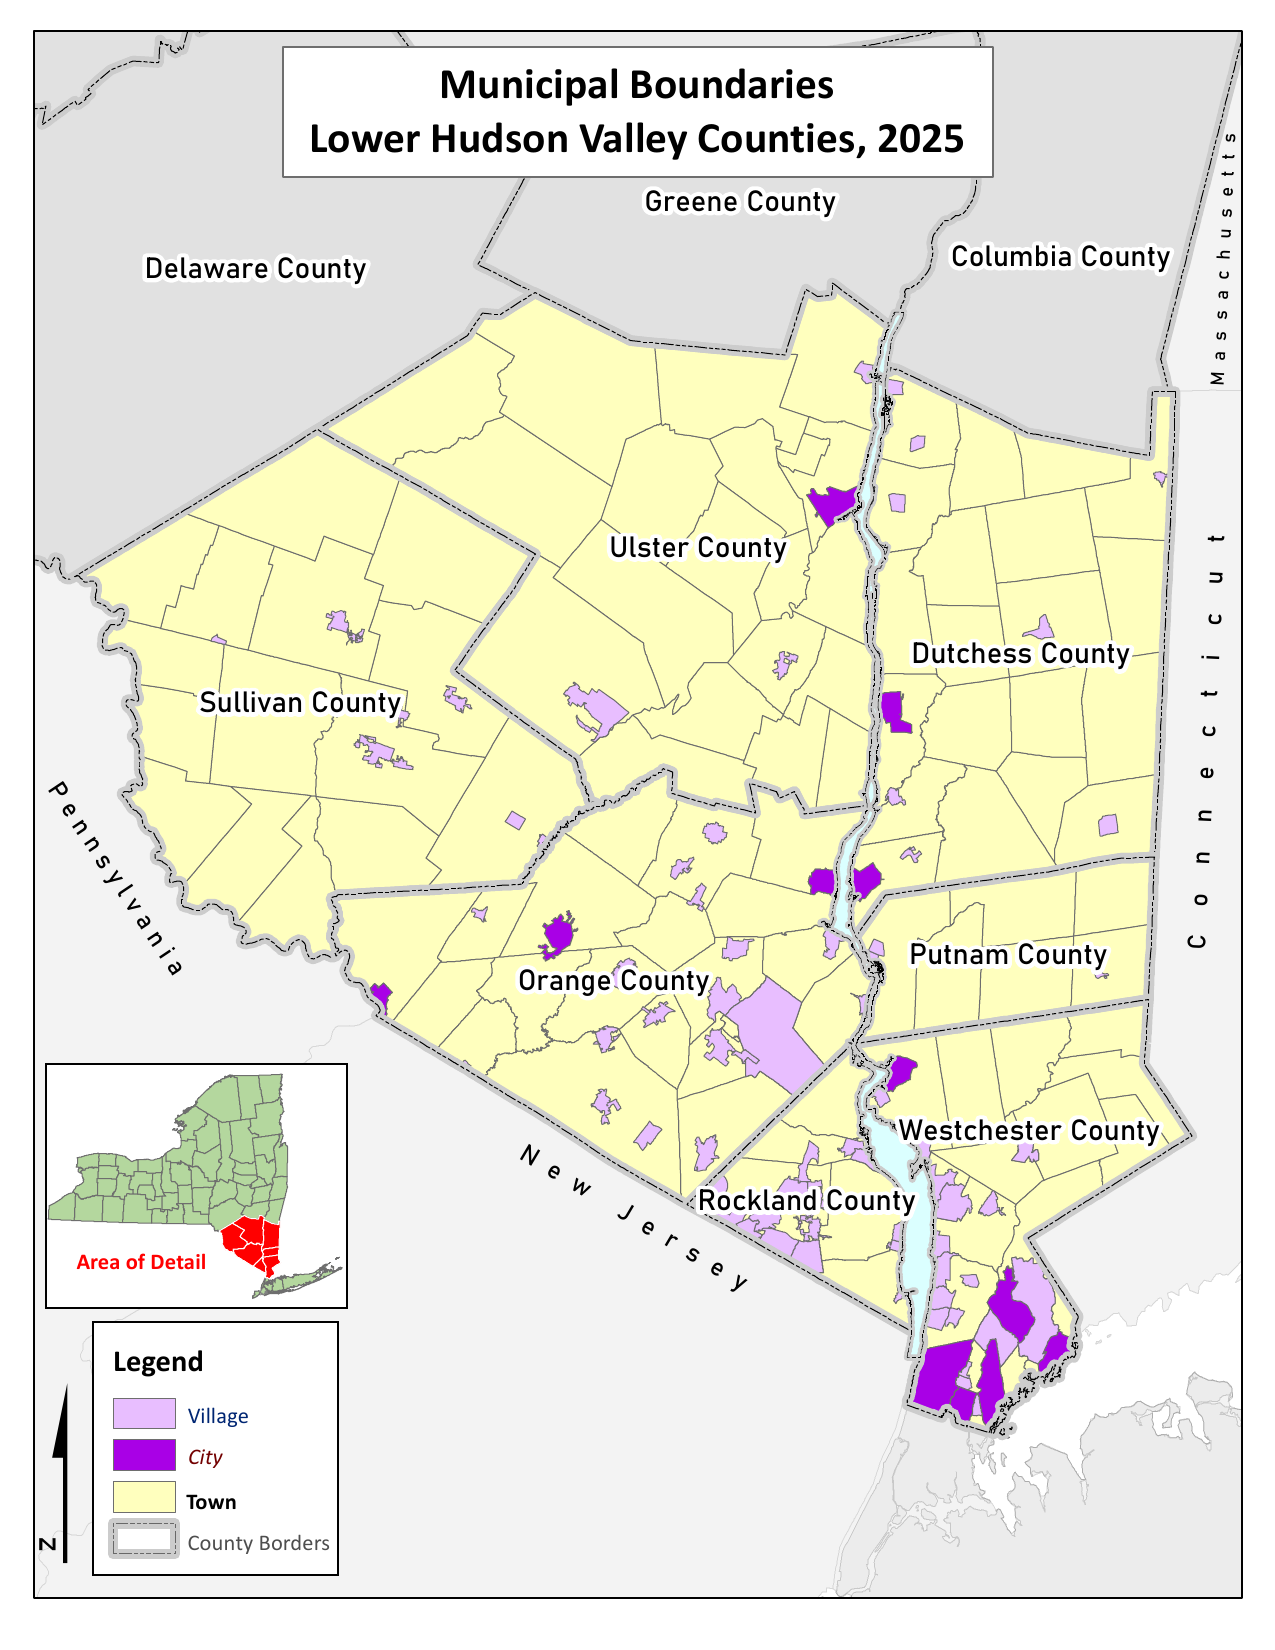
\includegraphics[width=1\linewidth,height=\textheight,keepaspectratio]{chapters/../media/appendix-maps/appendix-a-mid-hudson-region-map.png}
\href{../pdfs/CHA\%20Map/2025\%20CHA\%20County\%20Municipality\%20Maps_All_Part1.pdf}{Open
full PDF}

\section{Appendix B - Dutchess County Map}\label{sec-appendix-b-map}

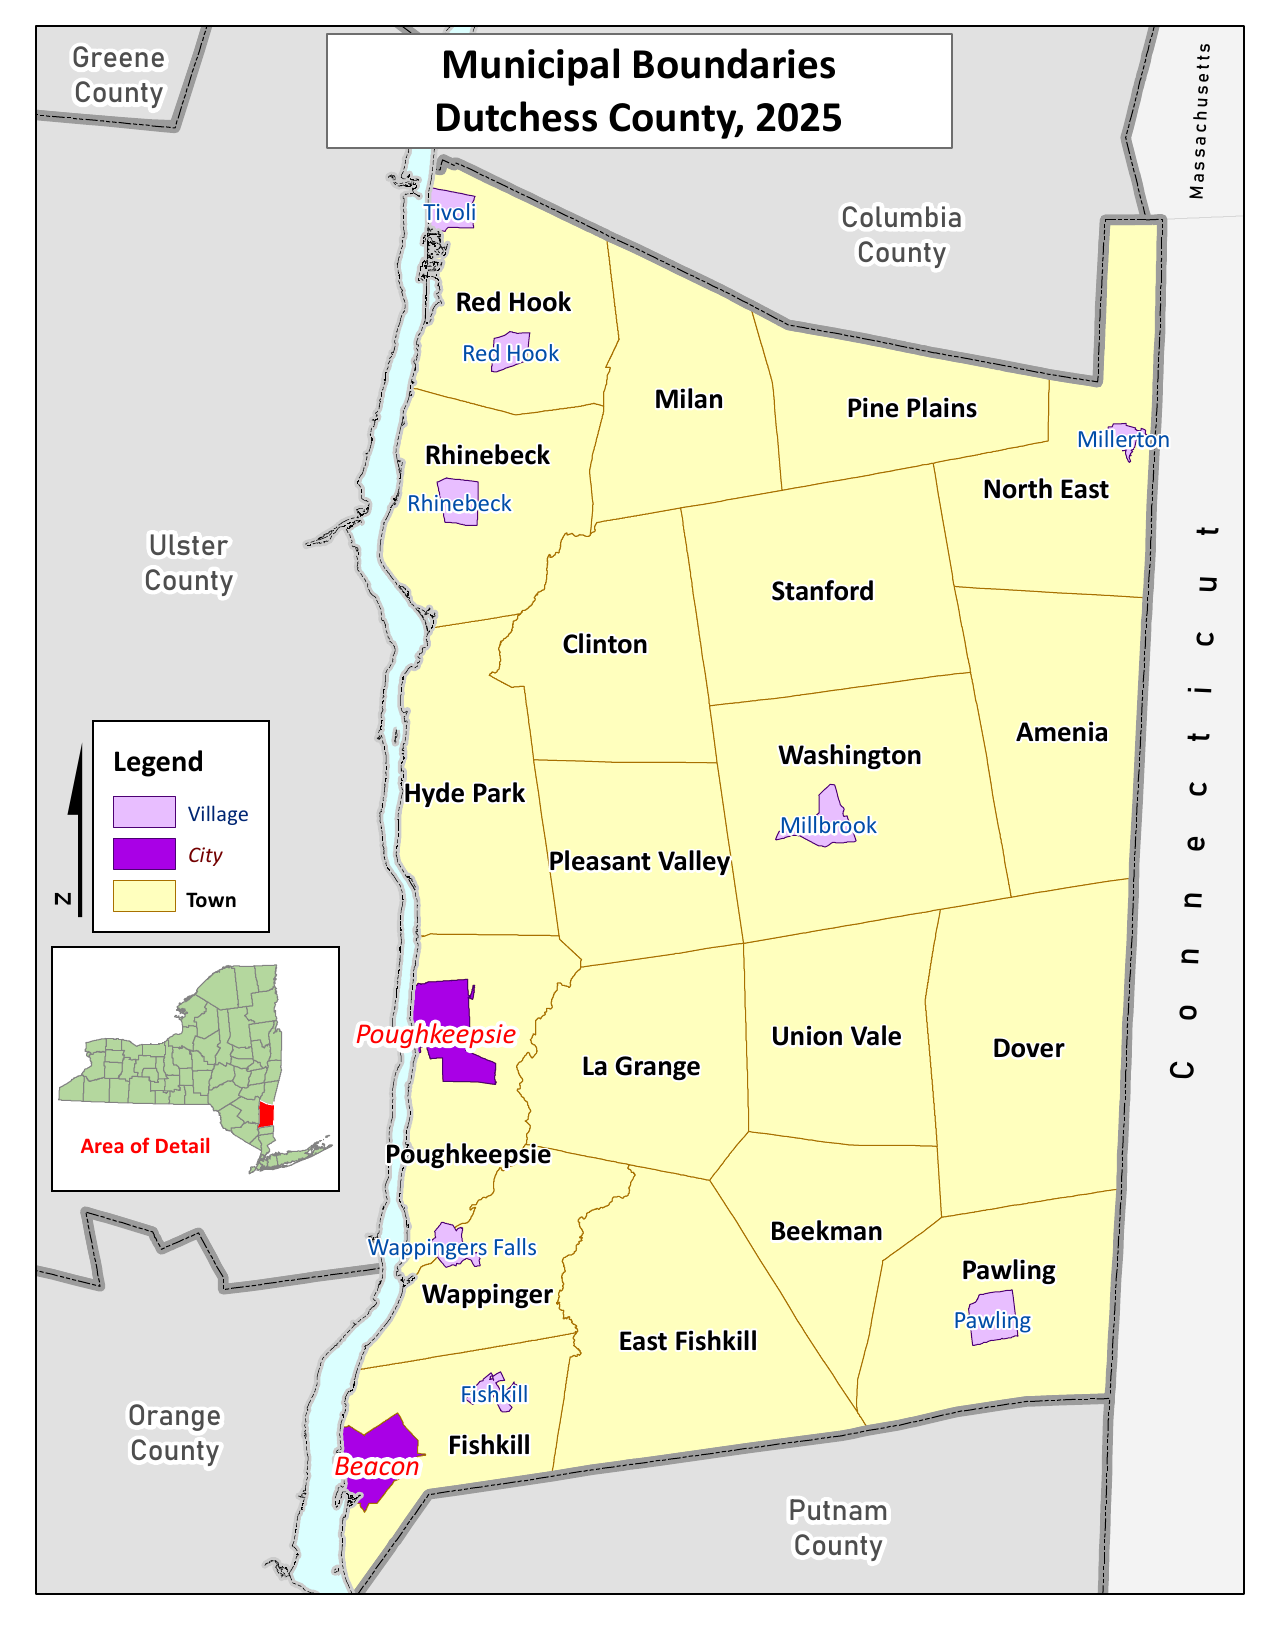
\includegraphics[width=1\linewidth,height=\textheight,keepaspectratio]{chapters/../media/appendix-maps/appendix-b-dutchess-county-map.png}
\href{../pdfs/CHA\%20Map/2025\%20CHA\%20County\%20Municipality\%20Maps_All_Part2.pdf}{Open
full PDF}

\section{Appendix C - Putnam County Map}\label{sec-appendix-c-map}

\includegraphics[width=1\linewidth,height=\textheight,keepaspectratio]{chapters/../media/appendix-maps/appendix-c-putnam-county-map.png}
\href{../pdfs/CHA\%20Map/2025\%20CHA\%20County\%20Municipality\%20Maps_All_Part3.pdf}{Open
full PDF}

\section{Appendix D - Westchester County Map}\label{sec-appendix-d-map}

\includegraphics[width=1\linewidth,height=\textheight,keepaspectratio]{chapters/../media/appendix-maps/appendix-d-westchester-county-map.png}
\href{../pdfs/CHA\%20Map/2025\%20CHA\%20County\%20Municipality\%20Maps_All_Part4.pdf}{Open
full PDF}

\section{Appendix E - Rockland County Map}\label{sec-appendix-e-map}

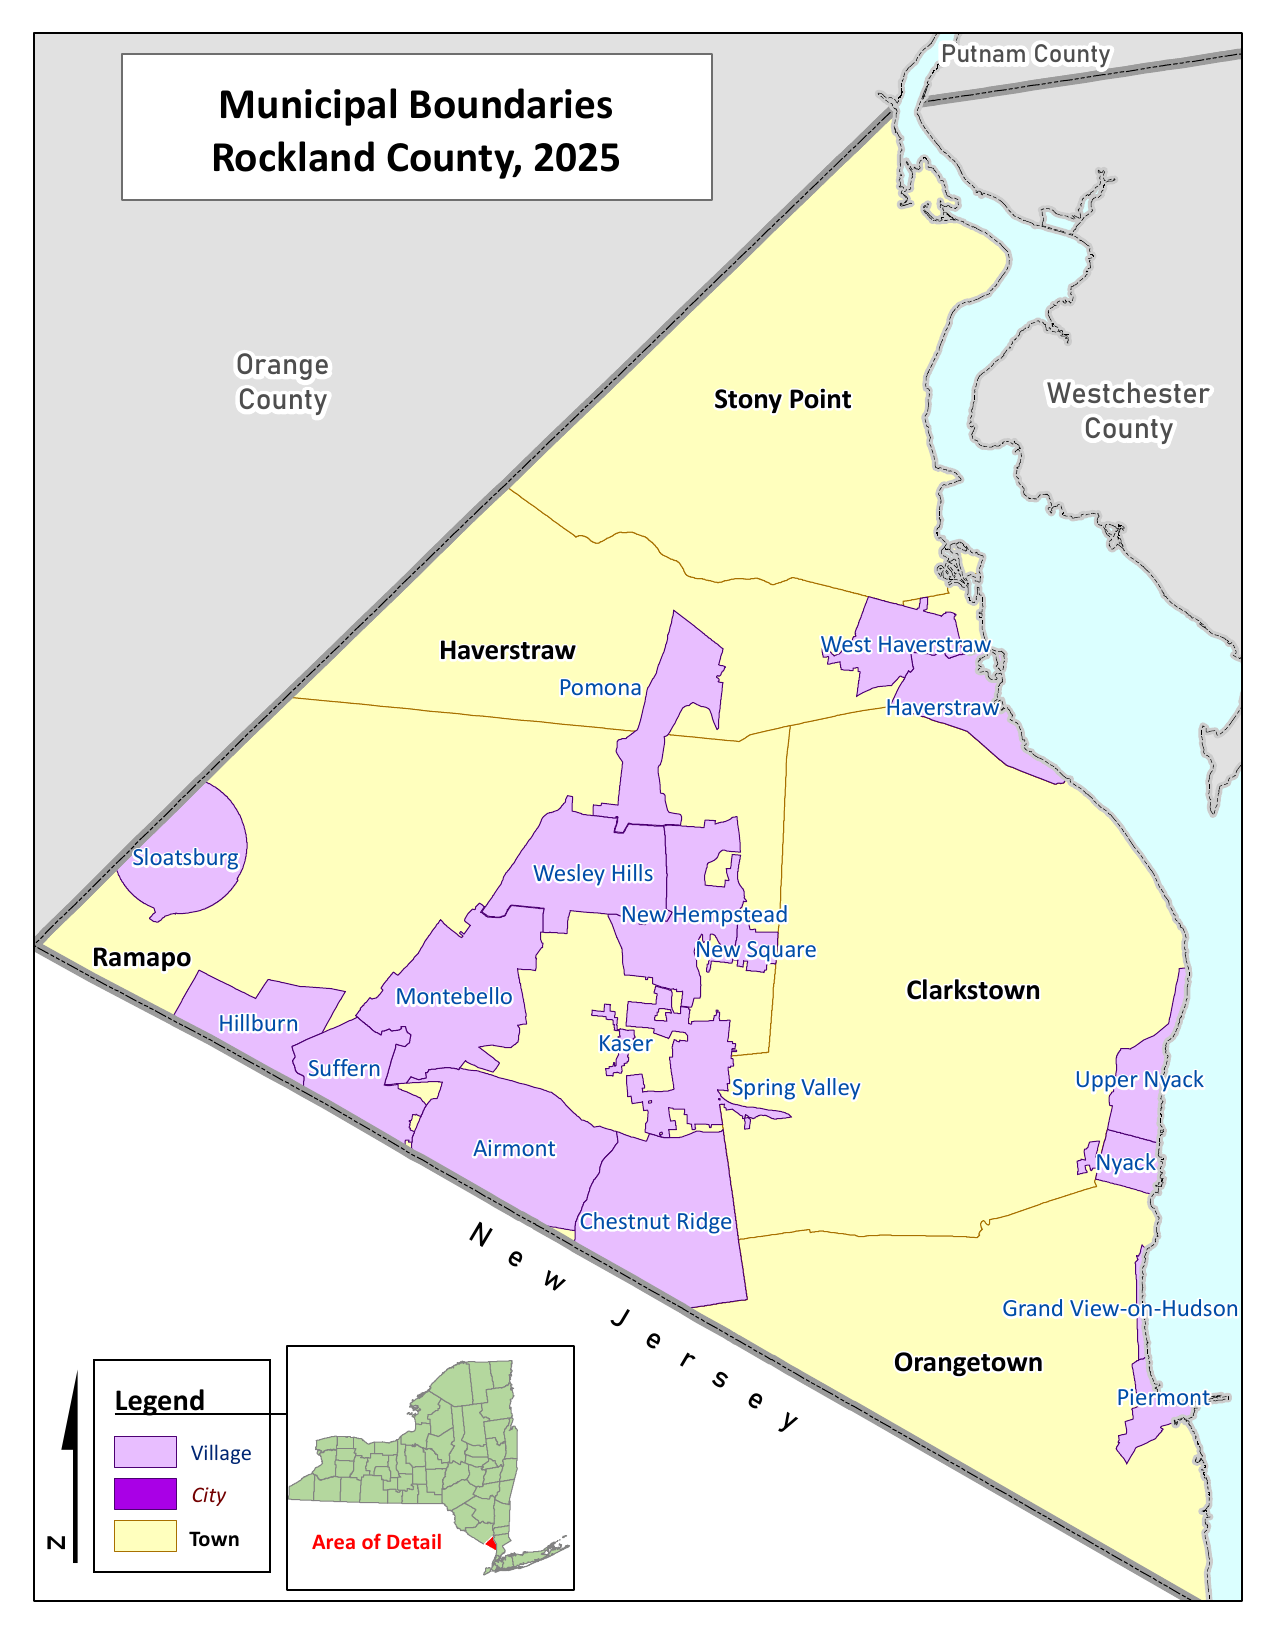
\includegraphics[width=1\linewidth,height=\textheight,keepaspectratio]{chapters/../media/appendix-maps/appendix-e-rockland-county-map.png}
\href{../pdfs/CHA\%20Map/2025\%20CHA\%20County\%20Municipality\%20Maps_All_Part5.pdf}{Open
full PDF}

\section{Appendix F - Orange County Map}\label{sec-appendix-f-map}

\includegraphics[width=1\linewidth,height=\textheight,keepaspectratio]{chapters/../media/appendix-maps/appendix-f-orange-county-map.png}
\href{../pdfs/CHA\%20Map/2025\%20CHA\%20County\%20Municipality\%20Maps_All_Part6.pdf}{Open
full PDF}

\section{Appendix G - Sullivan County Map}\label{sec-appendix-g-map}

\includegraphics[width=1\linewidth,height=\textheight,keepaspectratio]{chapters/../media/appendix-maps/appendix-g-sullivan-county-map.png}
\href{../pdfs/CHA\%20Map/2025\%20CHA\%20County\%20Municipality\%20Maps_All_Part7.pdf}{Open
full PDF}

\section{Appendix H - Ulster County Map}\label{sec-appendix-h-map}

\includegraphics[width=1\linewidth,height=\textheight,keepaspectratio]{chapters/../media/appendix-maps/appendix-h-ulster-county-map.png}
\href{../pdfs/CHA\%20Map/2025\%20CHA\%20County\%20Municipality\%20Maps_All_Part8.pdf}{Open
full PDF}

\section{Appendix I - Mid-Hudson Region Community Partner
Survey}\label{sec-appendix-i-community-partner-survey}

\href{../media/appendix-docs/I\%20-\%20Community\%20Provider\%20Survey\%202025.pdf}{Mid-Hudson
Region Community Partner Survey}

\section{Appendix J - Mid-Hudson Region Community Partner Survey
References}\label{sec-appendix-j-community-partner-survey-references}

\href{../media/appendix-docs/Mid-Hudson\%20Region\%20Community\%20Partner\%20Survey\%20References.pdf}{Mid-Hudson
Region Community Partner Survey References}

\section{Appendix K - Putnam County and Nuvance CBO and Partner
Survey}\label{sec-appendix-k-putnam-nuvance-cbo-survey}

\href{../media/appendix-docs/K\%20-\%20Putnam\%20CBO\%20Survey_English_FINAL.pdf}{Putnam
County and Nuvance CBO and Partner Survey}

\section{Appendix L - Mid-Hudson Regional Community Health
Survey}\label{sec-appendix-l-mid-hudson-regional-community-health-survey}

\href{../media/appendix-docs/L\%20-\%20Dutchess\%20and\%20Putnam\%20HVHealth0325_FinalQnaire.pdf}{Mid-Hudson
Regional Community Health Survey}

\section{Appendix M - Orange County Community Health
Survey}\label{sec-appendix-m-orange-county-community-health-survey}

\href{../media/appendix-docs/M\%20-\%202024\%20Script\%20(0524OCHealthWeb_Prn).pdf}{Orange
County Community Health Survey}

\section{Appendix N - Orange County Community Asset
Survey}\label{sec-appendix-n-orange-county-community-asset-survey}

\href{../media/appendix-docs/N\%20-\%20Community\%20Asset\%20Survey\%20ENG.pdf}{Orange
County Community Asset Survey}

\section{Appendix O - Putnam County and Nuvance Community Health
Experience
Survey}\label{sec-appendix-o-putnam-nuvance-community-health-experience-survey}

\href{../media/appendix-docs/O\%20-\%20Putnam\%20Community\%20Health\%20Experience\%20Survey_English.pdf}{Putnam
County and Nuvance Community Health Experience Survey}

\section{Appendix P - Rockland County Community Health Assessment
Survey}\label{sec-appendix-p-rockland-county-community-health-assessment-survey}

\href{../media/appendix-docs/P\%20-\%20Rockland\%20Community\%20Health\%20Assessment\%20Survey_English\%20Paper\%20Version.pdf}{Rockland
County Community Health Assessment Survey}

\section{Appendix Q - Greater New York Hospital Association 2025
Community Health Needs Assessment
Survey}\label{sec-appendix-q-gnyha-2025-community-health-needs-assessment-survey}

\href{../media/appendix-docs/Q\%20-\%202025\%20CHNA\%20Collab\%20Survey_English.pdf}{Greater
New York Hospital Association 2025 Community Health Needs Assessment
Survey}

\phantomsection\label{refs}
\begin{CSLReferences}{0}{1}
\bibitem[\citeproctext]{ref-nysdoh-prevention-agenda-2025}
\CSLLeftMargin{1. }%
\CSLRightInline{New York State Department of Health. Prevention agenda
2025-2030: New york state's health improvement plan {[}Internet{]}. 2025
{[}cited 2025 May{]}. Available from:
\url{https://www.health.ny.gov/prevention/prevention_agenda/2025-2030/}}

\bibitem[\citeproctext]{ref-hp2030-sdoh-overview-2025}
\CSLLeftMargin{2. }%
\CSLRightInline{U.S. Department of Health and Human Services, Office of
Disease Prevention and Health Promotion. Healthy people 2030: Social
determinants of health {[}Internet{]}. 2025 {[}cited 2025 Jun{]}.
Available from:
\url{https://health.gov/healthypeople/objectives-and-data/social-determinants-health}}

\bibitem[\citeproctext]{ref-irs-501c3-exemption-2025}
\CSLLeftMargin{3. }%
\CSLRightInline{Internal Revenue Service. Exemption requirements -
501(c)(3) organizations {[}Internet{]}. 2025 {[}cited 2025 Jun{]}.
Available from:
\url{https://www.irs.gov/charities-non-profits/charitable-organizations/exemption-requirements-501c3-organizations}}

\bibitem[\citeproctext]{ref-irs-revenue-ruling-69-545-1969}
\CSLLeftMargin{4. }%
\CSLRightInline{Internal Revenue Service. Revenue ruling 69-545
{[}Internet{]}. 1969 {[}cited 2025 Jun{]}. Available from:
\url{https://www.irs.gov/pub/irs-tege/rr69-545.pdf}}

\bibitem[\citeproctext]{ref-irs-501r3-chna-2025}
\CSLLeftMargin{5. }%
\CSLRightInline{Internal Revenue Service. Community health needs
assessment for charitable hospital organizations - section 501(r)(3)
{[}Internet{]}. 2025 {[}cited 2025 Jun{]}. Available from:
\url{https://www.irs.gov/charities-non-profits/community-health-needs-assessment-for-charitable-hospital-organizations-section-501r3}}

\bibitem[\citeproctext]{ref-us-census-decennial-population-2025}
\CSLLeftMargin{6. }%
\CSLRightInline{United States Census Bureau. Decennial population table
DECENNIALSF12010.P1 {[}Internet{]}. 2025 {[}cited 2025 Aug{]}. Available
from:
\url{https://data.census.gov/cedsci/table?q=decennial\%20population&g=0500000US36027\%248600000,36071\%248600000,36079\%248600000,36087\%248600000,36105\%248600000,36111\%248600000,36119\%248600000&d=DEC\%20Summary\%20File\%201&tid=DECENNIALSF12010.P1}}

\bibitem[\citeproctext]{ref-rwjf-employment-2013}
\CSLLeftMargin{7. }%
\CSLRightInline{Robert Wood Johnson Foundation. How does employment, or
unemployment, affect health? {[}Internet{]}. 2013 {[}cited 2025 Aug{]}.
Available from:
\url{https://www.rwjf.org/en/library/research/2012/12/how-does-employment--or-unemployment--affect-health-.html}}

\bibitem[\citeproctext]{ref-blinded-veterans-transition-2019}
\CSLLeftMargin{8. }%
\CSLRightInline{Blinded Veterans Association. Challenges veterans face
when leaving the military {[}Internet{]}. 2019 {[}cited 2025 Aug{]}.
Available from:
\url{https://bva.org/challenges-veterans-face-when-leaving-the-military/}}

\bibitem[\citeproctext]{ref-cdc-disability-overview-2025}
\CSLLeftMargin{9. }%
\CSLRightInline{Centers for Disease Control and Prevention. Disability
and health overview {[}Internet{]}. 2025 {[}cited 2025 Aug{]}. Available
from: \url{https://www.cdc.gov/disability-and-health/about/}}

\bibitem[\citeproctext]{ref-nysdoh-disability-report-2019}
\CSLLeftMargin{10. }%
\CSLRightInline{New York State Department of Health. Information for
action report {[}Internet{]}. 2019 {[}cited 2025 Aug{]}. Available from:
\url{https://www.health.ny.gov/statistics/prevention/injury_prevention/information_for_action/docs/2019-12_ifa_report.pdf}}

\bibitem[\citeproctext]{ref-feeding-america-map-2025}
\CSLLeftMargin{11. }%
\CSLRightInline{Feeding America. Map the meal gap: New york
{[}Internet{]}. 2025 {[}cited 2025 Aug{]}. Available from:
\url{https://map.feedingamerica.org/district/2023/overall/new-york}}

\bibitem[\citeproctext]{ref-feeding-america-meal-gap-2023}
\CSLLeftMargin{12. }%
\CSLRightInline{Feeding America. Map the meal gap 2023 {[}Internet{]}.
2023 {[}cited 2025 Aug{]}. Available from:
\url{https://www.feedingamerica.org/sites/default/files/2023-05/Map\%20the\%20Meal\%20Gap\%202023.pdf}}

\bibitem[\citeproctext]{ref-atlantic-homelessness-2016}
\CSLLeftMargin{13. }%
\CSLRightInline{The Atlantic. How health and homelessness are connected
{[}Internet{]}. 2016 {[}cited 2025 Aug{]}. Available from:
\url{https://www.theatlantic.com/politics/archive/2016/01/how-health-and-homelessness-are-connectedmedically/458871/}}

\bibitem[\citeproctext]{ref-urban-institute-housing-asthma-2017}
\CSLLeftMargin{14. }%
\CSLRightInline{Urban Institute, The National Center for Health in
Public Housing. Housing and asthma among school-age children living in
public housing {[}Internet{]}. 2017 {[}cited 2025 Aug{]}. Available
from:
\url{https://nchph.org/wp-content/uploads/2017/10/UI-2017-Housing-andAsthma-among-School-Age-Children-AHS-2015-1.pdf}}

\bibitem[\citeproctext]{ref-housing-infographic-2022}
\CSLLeftMargin{15. }%
\CSLRightInline{Mid-Hudson Region Housing Initiative. Housing
infographic {[}Internet{]}. 2022 {[}cited 2025 Aug{]}. Available from:
\url{https://infograph.venngage.com/ps/BDxQHEPVBXs/housing}}

\bibitem[\citeproctext]{ref-jchs-state-nations-housing-2017}
\CSLLeftMargin{16. }%
\CSLRightInline{Joint Center for Housing Studies of Harvard University.
The state of the nation's housing 2017 {[}Internet{]}. 2017 {[}cited
2025 Aug{]}. Available from:
\url{https://www.jchs.harvard.edu/sites/default/files/harvard_jchs_state_of_the_nations_housing_2017_chap6.pdf}}

\bibitem[\citeproctext]{ref-census-poverty-measures-guidance-2025}
\CSLLeftMargin{17. }%
\CSLRightInline{United States Census Bureau. How the census bureau
measures poverty {[}Internet{]}. 2025 {[}cited 2025 Aug{]}. Available
from:
\url{https://www.census.gov/topics/income-poverty/poverty/guidance/poverty-measures.html}}

\bibitem[\citeproctext]{ref-world-pop-review-family-size-2025}
\CSLLeftMargin{18. }%
\CSLRightInline{World Population Review. Average family size by state
{[}Internet{]}. 2025 {[}cited 2025 Aug{]}. Available from:
\url{https://worldpopulationreview.com/state-rankings/average-family-size-by-state}}

\bibitem[\citeproctext]{ref-hp2030-poverty-2025}
\CSLLeftMargin{19. }%
\CSLRightInline{U.S. Department of Health and Human Services, Office of
Disease Prevention and Health Promotion. Healthy people 2030: poverty
{[}Internet{]}. 2025 {[}cited 2025 Aug{]}. Available from:
\url{https://health.gov/healthypeople/priority-areas/social-determinants-health/literature-summaries/poverty}}

\bibitem[\citeproctext]{ref-nyscaa-poverty-report-2024}
\CSLLeftMargin{20. }%
\CSLRightInline{New York State Community Action Association. Annual
poverty report {[}Internet{]}. 2024 {[}cited 2025 Aug{]}. Available
from:
\url{https://nyscaa.memberclicks.net/assets/docs/PovReport2024/2024\%20NYS\%20Poverty\%20Report.pdf}}

\bibitem[\citeproctext]{ref-health-poverty-action-2018}
\CSLLeftMargin{21. }%
\CSLRightInline{Health Poverty Action. Key facts: Poverty and poor
health {[}Internet{]}. 2018 {[}cited 2025 Aug{]}. Available from:
\url{https://www.healthpovertyaction.org/news-events/key-facts-poverty-and-poor-health/}}

\bibitem[\citeproctext]{ref-aerj-ses-child-development-2011}
\CSLLeftMargin{22. }%
\CSLRightInline{American Educational Research Journal. Socioeconomic
status and child development. American Educational Research Journal
{[}Internet{]}. 2011 {[}cited 2025 Aug{]}. Available from:
\url{https://pmc.ncbi.nlm.nih.gov/articles/PMC2920529/}}

\bibitem[\citeproctext]{ref-united-for-alice-2020}
\CSLLeftMargin{23. }%
\CSLRightInline{United For ALICE. ALICE in the crosscurrents: COVID and
financial hardship in the united states {[}Internet{]}. 2020 {[}cited
2025 Aug{]}. Available from:
\url{https://www.unitedforalice.org/national-overview}}

\bibitem[\citeproctext]{ref-hp2030-high-school-graduation-2025}
\CSLLeftMargin{24. }%
\CSLRightInline{U.S. Department of Health and Human Services, Office of
Disease Prevention and Health Promotion. Healthy people 2030: High
school graduation {[}Internet{]}. 2025 {[}cited 2025 Aug{]}. Available
from:
\url{https://health.gov/healthypeople/priority-areas/social-determinants-health/literature-summaries/high-school-graduation}}

\bibitem[\citeproctext]{ref-learning-policy-institute-suspensions-2022}
\CSLLeftMargin{25. }%
\CSLRightInline{Learning Policy Institute. Pushed out: Trends and
disparities in out-of-school suspensions {[}Internet{]}. 2022 {[}cited
2025 Aug{]}. Available from:
\url{https://learningpolicyinstitute.org/product/crdc-school-suspension-report}}

\bibitem[\citeproctext]{ref-cdc-child-development-2024}
\CSLLeftMargin{26. }%
\CSLRightInline{Centers for Disease Control and Prevention. Child
development: facts {[}Internet{]}. 2024 {[}cited 2025 Aug{]}. Available
from: \url{https://www.cdc.gov/childdevelopment/about/}}

\bibitem[\citeproctext]{ref-who-parenting-interventions-2024}
\CSLLeftMargin{27. }%
\CSLRightInline{World Health Organization. Designing, implementing,
evaluating, and scaling up parenting interventions: A handbook for
decision-makers and implementers {[}Internet{]}. 2024 {[}cited 2025
Aug{]}. Available from:
\url{https://iris.who.int/bitstream/handle/10665/378237/9789240095595-eng.pdf}}

\bibitem[\citeproctext]{ref-who-nurturing-care-framework-2020}
\CSLLeftMargin{28. }%
\CSLRightInline{World Health Organization. Improving early childhood
development: WHO, UNICEF, and world bank group nurturing care framework
{[}Internet{]}. 2020 {[}cited 2025 Aug{]}. Available from:
\url{https://apps.who.int/iris/bitstream/handle/10665/331306/9789240002098-eng.pdf}}

\bibitem[\citeproctext]{ref-hp2030-early-childhood-2025}
\CSLLeftMargin{29. }%
\CSLRightInline{U.S. Department of Health and Human Services, Office of
Disease Prevention and Health Promotion. Healthy people 2030: Early
childhood development and education {[}Internet{]}. 2025 {[}cited 2025
Aug{]}. Available from:
\url{https://health.gov/healthypeople/priority-areas/social-determinants-health/literature-summaries/early-childhood-development-and-education}}

\bibitem[\citeproctext]{ref-cdc-preventing-aces-2019}
\CSLLeftMargin{30. }%
\CSLRightInline{Centers for Disease Control and Prevention, National
Center for Injury Prevention and Control, Division of Violence
Prevention. Preventing adverse childhood experiences (ACEs): Leveraging
the best available evidence {[}Internet{]}. 2019 {[}cited 2025 Aug{]}.
Available from:
\url{https://www.cdc.gov/violenceprevention/pdf/preventingACES.pdf}}

\bibitem[\citeproctext]{ref-hp2030-higher-education-2025}
\CSLLeftMargin{31. }%
\CSLRightInline{U.S. Department of Health and Human Services, Office of
Disease Prevention and Health Promotion. Healthy people 2030: Enrollment
in higher education {[}Internet{]}. 2025 {[}cited 2025 Aug{]}. Available
from:
\url{https://odphp.health.gov/healthypeople/priority-areas/social-determinants-health/literature-summaries/enrollment-higher-education}}

\bibitem[\citeproctext]{ref-ssa-education-earnings-2015}
\CSLLeftMargin{32. }%
\CSLRightInline{Social Security Administration. Research summary:
Education and lifetime earnings {[}Internet{]}. 2015 {[}cited 2025
Aug{]}. Available from:
\url{https://www.ssa.gov/policy/docs/research-summaries/education-earnings.html}}

\bibitem[\citeproctext]{ref-hp2030-language-literacy-2025}
\CSLLeftMargin{33. }%
\CSLRightInline{U.S. Department of Health and Human Services, Office of
Disease Prevention and Health Promotion. Healthy people 2030: Language
and literacy {[}Internet{]}. 2025 {[}cited 2025 Aug{]}. Available from:
\url{https://health.gov/healthypeople/priority-areas/social-determinants-health/literature-summaries/language-and-literacy}}

\bibitem[\citeproctext]{ref-hp2030-civic-participation-2025}
\CSLLeftMargin{34. }%
\CSLRightInline{U.S. Department of Health and Human Services, Office of
Disease Prevention and Health Promotion. Healthy people 2030: Civic
participation {[}Internet{]}. 2025 {[}cited 2025 Aug{]}. Available from:
\url{https://health.gov/healthypeople/priority-areas/social-determinants-health/literature-summaries/civic-participation}}

\bibitem[\citeproctext]{ref-uwphi-disconnected-youth-2022}
\CSLLeftMargin{35. }%
\CSLRightInline{University of Wisconsin Population Health Institute,
Robert Wood Johnson Foundation. Disconnected youth (ages 16-19) - county
health rankings definition {[}Internet{]}. 2022 {[}cited 2022 Sep{]}.
Available from:
\url{https://www.countyhealthrankings.org/app/new-york/2022/measure/factors/149/description}}

\bibitem[\citeproctext]{ref-measure-of-america-disconnected-youth-2025}
\CSLLeftMargin{36. }%
\CSLRightInline{Measure of America. Disconnected youth {[}Internet{]}.
2025 {[}cited 2025 Jul{]}. Available from:
\url{http://measureofamerica.org/disconnected-youth/}}

\bibitem[\citeproctext]{ref-usda-nifa-disconnected-youth-4h-2017}
\CSLLeftMargin{37. }%
\CSLRightInline{National Institute of Food and Agriculture, United
States Department of Agriculture, 4-H National Headquarters.
Disconnected youth fact sheet {[}Internet{]}. 2017 {[}cited 2022 Jul{]}.
Available from:
\url{https://www.nifa.usda.gov/sites/default/files/resource/disconnected-youth-fact-sheet-2017-08-11.pdf}}

\bibitem[\citeproctext]{ref-nih-structural-racism-discrimination-2021}
\CSLLeftMargin{38. }%
\CSLRightInline{National Institutes of Health, National Institute on
Minority Health and Health Disparities. Understanding and addressing the
impact of structural racism and discrimination on minority health and
health disparities (NOT-MD-21-016) --- key definitions {[}Internet{]}.
2021 {[}cited 2025 Aug{]}. Available from:
\url{https://grants.nih.gov/grants/guide/notice-files/NOT-MD-21-016.html}}

\bibitem[\citeproctext]{ref-cdc-racism-cancer-disparities-2025}
\CSLLeftMargin{39. }%
\CSLRightInline{Centers for Disease Control and Prevention. How racism
leads to cancer health disparities {[}Internet{]}. 2025 {[}cited 2025
Aug{]}. Available from:
\url{https://www.cdc.gov/cancer/healthequity/racism-health-disparities.html}}

\bibitem[\citeproctext]{ref-nih-phenx-discrimination-scales-2025}
\CSLLeftMargin{40. }%
\CSLRightInline{National Institutes of Health, National Institute on
Minority Health and Health Disparities. PhenX toolkit: Discrimination
major experiences and everyday discrimination scales {[}Internet{]}.
2025 {[}cited 2025 Aug{]}. Available from:
\url{https://www.phenxtoolkit.org/protocols/view/210302}}

\bibitem[\citeproctext]{ref-cdc-pcd-residential-segregation-2024}
\CSLLeftMargin{41. }%
\CSLRightInline{Centers for Disease Control and Prevention. Residential
segregation is a poignant example of environmental racism
{[}Internet{]}. 2024 {[}cited 2025 Aug{]}. Available from:
\url{https://www.cdc.gov/pcd/issues/2024/pdf/23_0248.pdf}}

\bibitem[\citeproctext]{ref-hud-fair-housing-discrimination-2025}
\CSLLeftMargin{42. }%
\CSLRightInline{U.S. Department of Housing and Urban Development.
Housing discrimination under the fair housing act {[}Internet{]}. 2025
{[}cited 2025 Aug{]}. Available from:
\url{https://www.hud.gov/helping-americans/fair-housing-act-overview}}

\bibitem[\citeproctext]{ref-uwphi-residential-segregation-bw-2025}
\CSLLeftMargin{43. }%
\CSLRightInline{University of Wisconsin Population Health Institute,
Robert Wood Johnson Foundation. Residential segregation (black-white)
{[}Internet{]}. 2025 {[}cited 2025 Aug{]}. Available from:
\url{https://www.countyhealthrankings.org/health-data/community-conditions/social-and-economic-factors/safety-and-social-support/residential-segregation-blackwhite?year=2025}}

\bibitem[\citeproctext]{ref-hhs-healthy-people-access-health-services-2025}
\CSLLeftMargin{44. }%
\CSLRightInline{U.S. Department of Health and Human Services, Office of
Disease Prevention and Health Promotion. Healthy people 2030: Access to
health services {[}Internet{]}. 2025 {[}cited 2025 Aug{]}. Available
from:
\url{https://odphp.health.gov/healthypeople/priority-areas/social-determinants-health/literature-summaries/access-health-services}}

\bibitem[\citeproctext]{ref-census-sipp-medical-debt-2023}
\CSLLeftMargin{45. }%
\CSLRightInline{U.S. Census Bureau. Survey of income and program
participation, survey year 2023, table 2 {[}Internet{]}. 2025 {[}cited
2025 Aug{]}. Available from:
\url{https://www.census.gov/data/tables/2023/demo/wealth/wealth-asset-ownership.html}}

\bibitem[\citeproctext]{ref-hp2030-crime-violence-2025}
\CSLLeftMargin{46. }%
\CSLRightInline{U.S. Department of Health and Human Services, Office of
Disease Prevention and Health Promotion. Healthy people 2030: Crime and
violence {[}Internet{]}. 2025 {[}cited 2025 Aug{]}. Available from:
\url{https://health.gov/healthypeople/priority-areas/social-determinants-health/literature-summaries/crime-and-violence}}

\bibitem[\citeproctext]{ref-hrsa-mua-mup-scoring-2022}
\CSLLeftMargin{47. }%
\CSLRightInline{U.S. Department of Health and Human Services, Health
Resources and Services Administration. Scoring shortage designations:
HPSA and MUAP scoring criteria {[}Internet{]}. 2022 {[}cited 2025
Aug{]}. Available from:
\url{https://www.hhs.gov/guidance/document/hpsa-and-muap-hpsa-scoring-criteria}}

\bibitem[\citeproctext]{ref-hp2030-access-primary-care-2025}
\CSLLeftMargin{48. }%
\CSLRightInline{U.S. Department of Health and Human Services, Office of
Disease Prevention and Health Promotion. Healthy people 2030: Access to
primary care {[}Internet{]}. 2025 {[}cited 2025 Aug{]}. Available from:
\url{https://odphp.health.gov/healthypeople/priority-areas/social-determinants-health/literature-summaries/access-primary-care}}

\bibitem[\citeproctext]{ref-acep-urgent-care-centers-2022}
\CSLLeftMargin{49. }%
\CSLRightInline{American College of Emergency Physicians. Urgent care
centers {[}Internet{]}. 2022 {[}cited 2025 Aug{]}. Available from:
\url{https://www.acep.org/patient-care/policy-statements/urgent-care-centers/}}

\bibitem[\citeproctext]{ref-skagit-urgent-vs-emergency-2025}
\CSLLeftMargin{50. }%
\CSLRightInline{Skagit Regional Health. When to use urgent care vs.
Emergency department {[}Internet{]}. 2025 {[}cited 2025 Aug{]}.
Available from:
\url{https://www.skagitregionalhealth.org/programs-services/urgent-care/when-to-use-urgent-care}}

\bibitem[\citeproctext]{ref-rand-ed-evolving-role-2013}
\CSLLeftMargin{51. }%
\CSLRightInline{Hsia, Renee Y., Gilbreath, Emily. The evolving role of
emergency departments in the united states. RAND Health Quarterly
{[}Internet{]}. 2013 {[}cited 2025 Aug{]}. Available from:
\url{https://pmc.ncbi.nlm.nih.gov/articles/PMC4945168/}}

\bibitem[\citeproctext]{ref-ahrq-pph-costs-2017}
\CSLLeftMargin{52. }%
\CSLRightInline{Agency for Healthcare Research and Quality.
Characteristics and costs of potentially preventable inpatient stays,
2017 {[}Internet{]}. 2017 {[}cited 2025 Aug{]}. Available from:
\url{https://hcup-us.ahrq.gov/reports/statbriefs/sb259-PotentiallyPreventable-Hospitalizations-2017.jsp}}

\bibitem[\citeproctext]{ref-hp2030-health-literacy-2025}
\CSLLeftMargin{53. }%
\CSLRightInline{U.S. Department of Health and Human Services, Office of
Disease Prevention and Health Promotion. Healthy people 2030: Health
literacy {[}Internet{]}. 2025 {[}cited 2025 Aug{]}. Available from:
\url{https://health.gov/healthypeople/priority-areas/health-literacy-healthy-people-2030}}

\bibitem[\citeproctext]{ref-who-health-literacy-2024}
\CSLLeftMargin{54. }%
\CSLRightInline{World Health Organization. Health literacy
{[}Internet{]}. 2024 {[}cited 2025 Aug{]}. Available from:
\url{https://www.who.int/news-room/fact-sheets/detail/health-literacy}}

\bibitem[\citeproctext]{ref-dietary-guidelines-2020-2025}
\CSLLeftMargin{55. }%
\CSLRightInline{U.S. Department of Agriculture, U.S. Department of
Health and Human Services. Dietary guidelines for americans, 2020-2025
{[}Internet{]}. 2020 {[}cited 2025 Jul{]}. Available from:
\url{https://www.dietaryguidelines.gov/sites/default/files/2021-03/Dietary_Guidelines_for_Americans-2020-2025.pdf}}

\bibitem[\citeproctext]{ref-cdc-chronic-disease-prevention-2022}
\CSLLeftMargin{56. }%
\CSLRightInline{Centers for Disease Control and Prevention. Chronic
disease prevention {[}Internet{]}. 2022 {[}cited 2025 Aug{]}. Available
from: \url{https://www.cdc.gov/chronic-disease/prevention/index.html}}

\bibitem[\citeproctext]{ref-cdc-living-with-chronic-disease-2024}
\CSLLeftMargin{57. }%
\CSLRightInline{Centers for Disease Control and Prevention. Living with
chronic disease {[}Internet{]}. 2024 {[}cited 2025 Aug{]}. Available
from: \url{https://www.cdc.gov/chronic-disease/living-with/index.html}}

\bibitem[\citeproctext]{ref-usda-ers-food-access-2025}
\CSLLeftMargin{58. }%
\CSLRightInline{U.S. Department of Agriculture, Economic Research
Service. Food access {[}Internet{]}. 2025 {[}cited 2025 Aug{]}.
Available from:
\url{https://www.ers.usda.gov/topics/food-choices-health/food-access/}}

\bibitem[\citeproctext]{ref-hp2030-access-foods-2025}
\CSLLeftMargin{59. }%
\CSLRightInline{U.S. Department of Health and Human Services, Office of
Disease Prevention and Health Promotion. Healthy people 2030: Access to
foods that support healthy eating patterns {[}Internet{]}. 2025 {[}cited
2025 Aug{]}. Available from:
\url{https://health.gov/healthypeople/priority-areas/social-determinants-health/literature-summaries/access-foods-support-healthy-eating-patterns\#cit14}}

\bibitem[\citeproctext]{ref-county-health-rankings-food-env-2025}
\CSLLeftMargin{60. }%
\CSLRightInline{University of Wisconsin Population Health Institute,
Robert Wood Johnson Foundation. County health rankings \& roadmaps: Food
environment index {[}Internet{]}. 2025 {[}cited 2025 Aug{]}. Available
from:
\url{https://www.countyhealthrankings.org/health-data/community-conditions/health-infrastructure/health-promotion-and-harm-reduction/food-environment-index?year=2025}}

\bibitem[\citeproctext]{ref-preventive-medicine-food-access-detroit-2015}
\CSLLeftMargin{61. }%
\CSLRightInline{National Library of Medicine. Detroit food environment
study (preventive medicine) {[}Internet{]}. 2015 {[}cited 2025 Aug{]}.
Available from: \url{https://pmc.ncbi.nlm.nih.gov/articles/PMC4134936/}}

\bibitem[\citeproctext]{ref-hp2030-environmental-conditions-2025}
\CSLLeftMargin{62. }%
\CSLRightInline{U.S. Department of Health and Human Services, Office of
Disease Prevention and Health Promotion. Healthy people 2030:
Environmental conditions {[}Internet{]}. 2025 {[}cited 2025 Aug{]}.
Available from:
\url{https://odphp.health.gov/healthypeople/priority-areas/social-determinants-health/literature-summaries/environmental-conditions}}

\bibitem[\citeproctext]{ref-epa-climate-vulnerable-2023}
\CSLLeftMargin{63. }%
\CSLRightInline{United States Environmental Protection Agency. EPA
report shows disproportionate impacts of climate change on socially
vulnerable populations {[}Internet{]}. 2023 {[}cited 2025 Aug{]}.
Available from:
\url{https://www.epa.gov/newsreleases/epa-report-shows-disproportionate-impacts-climate-change-socially-vulnerable}}

\bibitem[\citeproctext]{ref-county-health-rankings-air-pollution-factors-125-2022}
\CSLLeftMargin{64. }%
\CSLRightInline{University of Wisconsin Population Health Institute,
Robert Wood Johnson Foundation. Air pollution (fine particulate matter)
- county health rankings measure factors 125 {[}Internet{]}. 2022
{[}cited 2025 Aug{]}. Available from:
\url{https://www.countyhealthrankings.org/app/new-york/2022/measure/factors/125/description}}

\bibitem[\citeproctext]{ref-cdc-drinking-water-causes-2024}
\CSLLeftMargin{65. }%
\CSLRightInline{Centers for Disease Control and Prevention. Causes of
drinking water problems {[}Internet{]}. 2024 {[}cited 2025 Aug{]}.
Available from:
\url{https://www.cdc.gov/drinking-water/causes/index.html}}

\bibitem[\citeproctext]{ref-usgs-runoff-2018}
\CSLLeftMargin{66. }%
\CSLRightInline{U.S. Geological Survey. Runoff: Surface and overland
water runoff {[}Internet{]}. 2018 {[}cited 2025 Aug{]}. Available from:
\url{https://www.usgs.gov/special-topic/water-science-school/science/runoff-surface-and-overland-water-runoff?qt-science_center_objects=0\#qt-science_center_objects}}

\bibitem[\citeproctext]{ref-cdc-water-quality-health-2024}
\CSLLeftMargin{67. }%
\CSLRightInline{Centers for Disease Control and Prevention. Water
quality and your health {[}Internet{]}. 2024 {[}cited 2025 Aug{]}.
Available from:
\url{https://www.cdc.gov/drinking-water/about/water-quality-and-your-health.html}}

\bibitem[\citeproctext]{ref-cdc-lead-health-effects-2024}
\CSLLeftMargin{68. }%
\CSLRightInline{Centers for Disease Control and Prevention. Health
effects of lead exposure {[}Internet{]}. 2024 {[}cited 2025 Aug{]}.
Available from:
\url{https://www.cdc.gov/nceh/lead/prevention/health-effects.htm}}

\bibitem[\citeproctext]{ref-who-lead-poisoning-2024}
\CSLLeftMargin{69. }%
\CSLRightInline{World Health Organization. Lead poisoning and health
{[}Internet{]}. 2024 {[}cited 2025 Aug{]}. Available from:
\url{https://www.who.int/news-room/fact-sheets/detail/lead-poisoning-and-health}}

\bibitem[\citeproctext]{ref-cdc-lead-prevention-sources-2024}
\CSLLeftMargin{70. }%
\CSLRightInline{Centers for Disease Control and Prevention. Lead
prevention {[}Internet{]}. 2024 {[}cited 2025 Aug{]}. Available from:
\url{https://www.cdc.gov/lead-prevention/prevention/}}

\bibitem[\citeproctext]{ref-epa-childhood-lead-source-2024}
\CSLLeftMargin{71. }%
\CSLRightInline{United States Environmental Protection Agency. Most
significant source of childhood lead exposure in the residence
{[}Internet{]}. 2024 {[}cited 2025 Aug{]}. Available from:
\url{https://www.epa.gov/lead/what-most-significant-source-childhood-lead-exposure-residence}}

\bibitem[\citeproctext]{ref-cdc-lead-risk-factors-2024}
\CSLLeftMargin{72. }%
\CSLRightInline{Centers for Disease Control and Prevention. Lead
exposure risk factors {[}Internet{]}. 2024 {[}cited 2025 Aug{]}.
Available from: \url{https://www.cdc.gov/lead-prevention/risk-factors/}}

\bibitem[\citeproctext]{ref-nysdoh-lead-2025}
\CSLLeftMargin{73. }%
\CSLRightInline{New York State Department of Health. Lead poisoning
prevention {[}Internet{]}. 2025 {[}cited 2025 Aug{]}. Available from:
\url{https://www.health.ny.gov/environmental/lead/}}

\bibitem[\citeproctext]{ref-hp2030-quality-housing-2025}
\CSLLeftMargin{74. }%
\CSLRightInline{U.S. Department of Health and Human Services, Office of
Disease Prevention and Health Promotion. Healthy people 2030: Quality
housing {[}Internet{]}. 2025 {[}cited 2025 Aug{]}. Available from:
\url{https://health.gov/healthypeople/priority-areas/social-determinants-health/literature-summaries/quality-housing}}

\bibitem[\citeproctext]{ref-hp2030-transportation-2025}
\CSLLeftMargin{75. }%
\CSLRightInline{U.S. Department of Health and Human Services, Office of
Disease Prevention and Health Promotion. Healthy people 2030:
transportation {[}Internet{]}. 2025 {[}cited 2025 Aug{]}. Available
from:
\url{https://health.gov/healthypeople/objectives-and-data/browse-objectives/transportation}}

\bibitem[\citeproctext]{ref-sciencedirect-transport-access-healthcare-2020}
\CSLLeftMargin{76. }%
\CSLRightInline{Elsevier Ltd. Transportation access and health care
utilization {[}Internet{]}. 2020 {[}cited 2022 Aug{]}. Available from:
\url{https://reader.elsevier.com/reader/sd/pii/S2590198220301494}}

\bibitem[\citeproctext]{ref-harvard-commuting-productivity-2021}
\CSLLeftMargin{77. }%
\CSLRightInline{Harvard Business School. Commuting kills productivity
and your best talent suffers most {[}Internet{]}. 2021 {[}cited 2025
Aug{]}. Available from:
\url{https://hbswk.hbs.edu/item/commuting-kills-productivity-and-your-best-talent-suffers-most}}

\bibitem[\citeproctext]{ref-hhs-physical-activity-guidelines-2018}
\CSLLeftMargin{78. }%
\CSLRightInline{U.S. Department of Health and Human Services. Physical
activity guidelines for americans, 2nd edition {[}Internet{]}. 2018
{[}cited 2025 Jul{]}. Available from:
\url{https://health.gov/sites/default/files/2019-09/Physical_Activity_Guidelines_2nd_edition.pdf}}

\bibitem[\citeproctext]{ref-cdc-physical-activity-benefits-2024}
\CSLLeftMargin{79. }%
\CSLRightInline{Centers for Disease Control and Prevention. Benefits of
physical activity {[}Internet{]}. 2024 {[}cited 2025 Jul{]}. Available
from:
\url{https://www.cdc.gov/physical-activity-basics/benefits/index.html}}

\bibitem[\citeproctext]{ref-hp2030-physical-activity-2025}
\CSLLeftMargin{80. }%
\CSLRightInline{U.S. Department of Health and Human Services, Office of
Disease Prevention and Health Promotion. Healthy people 2030: Physical
activity {[}Internet{]}. 2025 {[}cited 2025 Jul{]}. Available from:
\url{https://health.gov/healthypeople/objectives-and-data/browse-objectives/physical-activity}}

\bibitem[\citeproctext]{ref-cdc-sugar-sweetened-beverages-2024}
\CSLLeftMargin{81. }%
\CSLRightInline{Centers for Disease Control and Prevention.
Sugar-sweetened beverages {[}Internet{]}. 2024 {[}cited 2025 Jul{]}.
Available from:
\url{https://www.cdc.gov/nutrition/php/data-research/sugar-sweetened-beverages.html}}

\bibitem[\citeproctext]{ref-jama-clrd-definitions-2021}
\CSLLeftMargin{82. }%
\CSLRightInline{JAMA Network Open. Respiratory diseases in the united
states {[}Internet{]}. 2021 {[}cited 2025 Jul{]}. Available from:
\url{https://jamanetwork.com/journals/jamanetworkopen/fullarticle/2786682}}

\bibitem[\citeproctext]{ref-cdc-data-brief-leading-causes-2024}
\CSLLeftMargin{83. }%
\CSLRightInline{Centers for Disease Control and Prevention. Data brief
521: Leading causes of death in the united states, 2023 {[}Internet{]}.
2024 {[}cited 2025 Jun{]}. Available from:
\url{https://www.cdc.gov/nchs/data/databriefs/db521.pdf}}

\bibitem[\citeproctext]{ref-nhlbi-asthma-causes-2024}
\CSLLeftMargin{84. }%
\CSLRightInline{National Heart, Lung, and Blood Institute. Causes of
asthma {[}Internet{]}. 2024 {[}cited 2025 Jun{]}. Available from:
\url{https://www.nhlbi.nih.gov/health/asthma/causes}}

\bibitem[\citeproctext]{ref-who-asthma-fact-sheet-2025}
\CSLLeftMargin{85. }%
\CSLRightInline{World Health Organization. Asthma {[}Internet{]}. 2025
{[}cited 2025 Jun{]}. Available from:
\url{https://www.who.int/news-room/fact-sheets/detail/asthma}}

\bibitem[\citeproctext]{ref-cdc-asthma-control-2024}
\CSLLeftMargin{86. }%
\CSLRightInline{Centers for Disease Control and Prevention. Asthma
control {[}Internet{]}. 2024 {[}cited 2025 Jun{]}. Available from:
\url{https://www.cdc.gov/asthma/control/index.html}}

\bibitem[\citeproctext]{ref-cdc-asthma-most-recent-national-data-2023}
\CSLLeftMargin{87. }%
\CSLRightInline{Centers for Disease Control and Prevention. Most recent
national asthma data {[}Internet{]}. 2023 {[}cited 2025 Jun{]}.
Available from:
\url{https://www.cdc.gov/asthma/most_recent_national_asthma_data.htm}}

\bibitem[\citeproctext]{ref-aha-cardiovascular-disease-2024}
\CSLLeftMargin{88. }%
\CSLRightInline{American Heart Association. What is cardiovascular
disease? {[}Internet{]}. 2024 {[}cited 2025 Jul{]}. Available from:
\url{https://www.heart.org/en/health-topics/consumer-healthcare/what-is-cardiovascular-disease}}

\bibitem[\citeproctext]{ref-cdc-heart-disease-factsstats-2024}
\CSLLeftMargin{89. }%
\CSLRightInline{Centers for Disease Control and Prevention. Heart
disease facts {[}Internet{]}. 2024 {[}cited 2025 Jul{]}. Available from:
\url{https://www.cdc.gov/heart-disease/data-research/factsstats/?CDC_AAref_Val=https://www.cdc.gov/heartdisease/facts.htm}}

\bibitem[\citeproctext]{ref-cdc-heart-disease-risk-factors-2024}
\CSLLeftMargin{90. }%
\CSLRightInline{Centers for Disease Control and Prevention. Risk factors
for heart disease {[}Internet{]}. 2024 {[}cited 2025 Jul{]}. Available
from: \url{https://www.cdc.gov/heart-disease/risk-factors/index.html}}

\bibitem[\citeproctext]{ref-cdc-heart-disease-mental-health-2024}
\CSLLeftMargin{91. }%
\CSLRightInline{Centers for Disease Control and Prevention. Heart
disease and mental health {[}Internet{]}. 2024 {[}cited 2025 Jul{]}.
Available from:
\url{https://www.cdc.gov/heart-disease/about/about-heart-disease-and-mentalhealth.html?CDC_AAref_Val=https://www.cdc.gov/heartdisease/mentalhealth.htm}}

\bibitem[\citeproctext]{ref-mayoclinic-high-blood-pressure-symptoms-causes-2024}
\CSLLeftMargin{92. }%
\CSLRightInline{Mayo Clinic. High blood pressure: Symptoms and causes
{[}Internet{]}. 2024 {[}cited 2025 Jun{]}. Available from:
\url{https://www.mayoclinic.org/diseases-conditions/high-blood-pressure/symptoms-causes/syc-20373410}}

\bibitem[\citeproctext]{ref-cdc-high-blood-pressure-factsstats-2024}
\CSLLeftMargin{93. }%
\CSLRightInline{Centers for Disease Control and Prevention. High blood
pressure: Facts and statistics {[}Internet{]}. 2024 {[}cited 2025
Jul{]}. Available from:
\url{https://www.cdc.gov/high-blood-pressure/data-research/factsstats/?CDC_AAref_Val=https://www.cdc.gov/bloodpressure/facts.htm}}

\bibitem[\citeproctext]{ref-cdc-high-blood-pressure-living-with-2024}
\CSLLeftMargin{94. }%
\CSLRightInline{Centers for Disease Control and Prevention. Living with
high blood pressure {[}Internet{]}. 2024 {[}cited 2025 Jul{]}. Available
from:
\url{https://www.cdc.gov/high-blood-pressure/living-with/index.html}}

\bibitem[\citeproctext]{ref-clevelandclinic-cerebrovascular-disease-2022}
\CSLLeftMargin{95. }%
\CSLRightInline{Cleveland Clinic. Cerebrovascular disease
{[}Internet{]}. 2022 {[}cited 2025 Jul{]}. Available from:
\url{https://my.clevelandclinic.org/health/diseases/24205-cerebrovascular-disease}}

\bibitem[\citeproctext]{ref-cdc-stroke-about-2024}
\CSLLeftMargin{96. }%
\CSLRightInline{Centers for Disease Control and Prevention. Stroke:
about {[}Internet{]}. 2024 {[}cited 2025 Jul{]}. Available from:
\url{https://www.cdc.gov/stroke/about/index.html}}

\bibitem[\citeproctext]{ref-mayo-clinic-stroke-symptoms-causes-2024}
\CSLLeftMargin{97. }%
\CSLRightInline{Mayo Clinic. Stroke: Symptoms and causes {[}Internet{]}.
2024 {[}cited 2025 Jul{]}. Available from:
\url{https://www.mayoclinic.org/diseases-conditions/stroke/symptoms-causes/syc-20350113}}

\bibitem[\citeproctext]{ref-cdc-stroke-risk-factors-2024}
\CSLLeftMargin{98. }%
\CSLRightInline{Centers for Disease Control and Prevention. Stroke risk
factors {[}Internet{]}. 2024 {[}cited 2025 Jul{]}. Available from:
\url{https://www.cdc.gov/stroke/riskfactors/?CDC_AAref_Val=https://www.cdc.gov/stroke/risk_factors.htm}}

\bibitem[\citeproctext]{ref-cdc-coronary-heart-disease-2021}
\CSLLeftMargin{99. }%
\CSLRightInline{Centers for Disease Control and Prevention. Coronary
heart disease {[}Internet{]}. 2021 {[}cited 2022 Sep{]}. Available from:
\url{https://www.cdc.gov/heartdisease/coronary_ad.htm}}

\bibitem[\citeproctext]{ref-mayo-coronary-artery-disease-symptoms-causes-2024}
\CSLLeftMargin{100. }%
\CSLRightInline{Mayo Clinic. Coronary artery disease: Symptoms and
causes {[}Internet{]}. 2024 {[}cited 2022 Sep{]}. Available from:
\url{https://www.mayoclinic.org/diseases-conditions/coronary-artery-disease/symptoms-causes/syc-20350613}}

\bibitem[\citeproctext]{ref-cdc-heart-attack-about-2024}
\CSLLeftMargin{101. }%
\CSLRightInline{Centers for Disease Control and Prevention. Heart attack
{[}Internet{]}. 2024 {[}cited 2025 Sep{]}. Available from:
\url{https://www.cdc.gov/heart-disease/about/heart-attack.html}}

\bibitem[\citeproctext]{ref-cdc-heart-disease-facts-stats-2024}
\CSLLeftMargin{102. }%
\CSLRightInline{Centers for Disease Control and Prevention. Heart
disease facts and statistics {[}Internet{]}. 2024 {[}cited 2025 Sep{]}.
Available from:
\url{https://www.cdc.gov/heart-disease/data-research/facts-stats/index.html}}

\bibitem[\citeproctext]{ref-mayoclinic-heart-attack-symptoms-causes-2023}
\CSLLeftMargin{103. }%
\CSLRightInline{Mayo Clinic. Heart attack: Symptoms and causes
{[}Internet{]}. 2023 {[}cited 2025 Sep{]}. Available from:
\url{https://www.mayoclinic.org/diseases-conditions/heart-attack/symptoms-causes/syc-20373106}}

\bibitem[\citeproctext]{ref-cdc-type-1-diabetes-2024}
\CSLLeftMargin{104. }%
\CSLRightInline{Centers for Disease Control and Prevention. About type 1
diabetes {[}Internet{]}. 2024 {[}cited 2025 Aug{]}. Available from:
\url{https://www.cdc.gov/diabetes/about/about-type-1-diabetes.html}}

\bibitem[\citeproctext]{ref-cdc-type-2-diabetes-2024}
\CSLLeftMargin{105. }%
\CSLRightInline{Centers for Disease Control and Prevention. About type 2
diabetes {[}Internet{]}. 2024 {[}cited 2025 Aug{]}. Available from:
\url{https://www.cdc.gov/diabetes/about/about-type-2-diabetes.html}}

\bibitem[\citeproctext]{ref-ada-about-diabetes-statistics-2022}
\CSLLeftMargin{106. }%
\CSLRightInline{American Diabetes Association. About diabetes
{[}Internet{]}. 2022 {[}cited 2025 Aug{]}. Available from:
\url{https://diabetes.org/about-us/statistics/about-diabetes}}

\bibitem[\citeproctext]{ref-nysdoh-diabetes-2025}
\CSLLeftMargin{107. }%
\CSLRightInline{New York State Department of Health. Diabetes
{[}Internet{]}. 2025 {[}cited 2025 Aug{]}. Available from:
\url{https://www.health.ny.gov/diseases/conditions/diabetes/}}

\bibitem[\citeproctext]{ref-ada-diabetes-basics-statistics-2022}
\CSLLeftMargin{108. }%
\CSLRightInline{American Diabetes Association. Diabetes statistics
{[}Internet{]}. 2022 {[}cited 2025 Oct{]}. Available from:
\url{http://www.diabetes.org/diabetes-basics/statistics/?loc=db-slabnav}}

\bibitem[\citeproctext]{ref-cdc-obesity-overview-2025}
\CSLLeftMargin{109. }%
\CSLRightInline{Centers for Disease Control and Prevention. Obesity
{[}Internet{]}. 2025 {[}cited 2025 Sep{]}. Available from:
\url{https://www.cdc.gov/obesity/index.html}}

\bibitem[\citeproctext]{ref-cdc-adult-obesity-facts-2025}
\CSLLeftMargin{110. }%
\CSLRightInline{Centers for Disease Control and Prevention. Adult
obesity facts {[}Internet{]}. 2025 {[}cited 2025 Sep{]}. Available from:
\url{https://www.cdc.gov/obesity/data/adult.html}}

\bibitem[\citeproctext]{ref-sinha-jastreboff-stress-obesity-2013}
\CSLLeftMargin{111. }%
\CSLRightInline{Rajita Sinha, Ania M. Jastreboff. Stress as a common
risk factor for obesity and addiction {[}Internet{]}. 2013 {[}cited 2025
Sep{]}. Available from:
\url{https://www.ncbi.nlm.nih.gov/pmc/articles/PMC3658316/}}

\bibitem[\citeproctext]{ref-nci-what-is-cancer-2021}
\CSLLeftMargin{112. }%
\CSLRightInline{National Cancer Institute. What is cancer?
{[}Internet{]}. 2021 {[}cited 2025 Jul{]}. Available from:
\url{https://www.cancer.gov/about-cancer/understanding/what-is-cancer}}

\bibitem[\citeproctext]{ref-nci-cancer-risk-factors-2015}
\CSLLeftMargin{113. }%
\CSLRightInline{National Cancer Institute. Risk factors for cancer
{[}Internet{]}. 2015 {[}cited 2025 Jul{]}. Available from:
\url{https://www.cancer.gov/about-cancer/causes-prevention/risk}}

\bibitem[\citeproctext]{ref-nysdoh-leading-causes-dashboard-2025}
\CSLLeftMargin{114. }%
\CSLRightInline{New York State Department of Health. Leading causes of
death dashboard {[}Internet{]}. 2025 {[}cited 2025 Jul{]}. Available
from:
\url{https://apps.health.ny.gov/public/tabvis/PHIG_Public/lcd/reports/\#county}}

\bibitem[\citeproctext]{ref-cdc-colorectal-cancer-overview-2022}
\CSLLeftMargin{115. }%
\CSLRightInline{Centers for Disease Control and Prevention. Colorectal
cancer {[}Internet{]}. 2022 {[}cited 2025 Jul{]}. Available from:
\url{https://www.cdc.gov/cancer/colorectal/index.htm}}

\bibitem[\citeproctext]{ref-cdc-colorectal-cancer-prevention-2025}
\CSLLeftMargin{116. }%
\CSLRightInline{Centers for Disease Control and Prevention. Colorectal
cancer prevention {[}Internet{]}. 2025 {[}cited 2025 Jul{]}. Available
from: \url{https://www.cdc.gov/colorectal-cancer/prevention/index.html}}

\bibitem[\citeproctext]{ref-uspstf-colorectal-cancer-screening-2021}
\CSLLeftMargin{117. }%
\CSLRightInline{U.S. Preventive Services Task Force. Colorectal cancer:
screening {[}Internet{]}. 2021 {[}cited 2025 Jul{]}. Available from:
\url{https://www.uspreventiveservicestaskforce.org/uspstf/recommendation/colorectal-cancer-screening}}

\bibitem[\citeproctext]{ref-cdc-colorectal-cancer-screening-2025}
\CSLLeftMargin{118. }%
\CSLRightInline{Centers for Disease Control and Prevention. Colorectal
cancer screening {[}Internet{]}. 2025 {[}cited 2025 Jul{]}. Available
from: \url{https://www.cdc.gov/colorectal-cancer/screening/index.html}}

\bibitem[\citeproctext]{ref-nysdoh-lung-cancer-about-2025}
\CSLLeftMargin{119. }%
\CSLRightInline{New York State Department of Health. Lung cancer
{[}Internet{]}. 2025 {[}cited 2025 Aug{]}. Available from:
\url{https://www.health.ny.gov/statistics/cancer/registry/abouts/lung.htm}}

\bibitem[\citeproctext]{ref-acs-radon-exposure-2022}
\CSLLeftMargin{120. }%
\CSLRightInline{American Cancer Society. Radon {[}Internet{]}. 2022
{[}cited 2025 Aug{]}. Available from:
\url{https://www.cancer.org/cancer/cancer-causes/radiation-exposure/radon.html}}

\bibitem[\citeproctext]{ref-cdc-prostate-cancer-2022}
\CSLLeftMargin{121. }%
\CSLRightInline{Centers for Disease Control and Prevention. Prostate
cancer {[}Internet{]}. 2022 {[}cited 2025 Aug{]}. Available from:
\url{https://www.cdc.gov/cancer/prostate/index.htm}}

\bibitem[\citeproctext]{ref-acs-how-common-breast-cancer-2022}
\CSLLeftMargin{122. }%
\CSLRightInline{American Cancer Society. How common is breast cancer?
{[}Internet{]}. 2022 {[}cited 2022 Jul{]}. Available from:
\url{https://www.cancer.org/cancer/breast-cancer/about/how-common-is-breast-cancer.html}}

\bibitem[\citeproctext]{ref-acs-newer-experimental-breast-imaging-2025}
\CSLLeftMargin{123. }%
\CSLRightInline{American Cancer Society. Newer and experimental breast
imaging tests {[}Internet{]}. 2025 {[}cited 2025 Aug{]}. Available from:
\url{https://www.cancer.org/cancer/types/breast-cancer/screening-tests-and-early-detection/mammograms/other-exams.html}}

\bibitem[\citeproctext]{ref-nci-cervical-cancer-overview-2023}
\CSLLeftMargin{124. }%
\CSLRightInline{National Cancer Institute. Cervical cancer
{[}Internet{]}. 2023 {[}cited 2025 Jul{]}. Available from:
\url{https://www.cancer.gov/types/cervical}}

\bibitem[\citeproctext]{ref-nci-cervical-cancer-symptoms-2022}
\CSLLeftMargin{125. }%
\CSLRightInline{National Cancer Institute. Cervical cancer symptoms
{[}Internet{]}. 2022 {[}cited 2025 Jul{]}. Available from:
\url{https://www.cancer.gov/types/cervical/symptoms}}

\bibitem[\citeproctext]{ref-nci-cervical-cancer-causes-risk-prevention-2024}
\CSLLeftMargin{126. }%
\CSLRightInline{National Cancer Institute. Cervical cancer: Causes, risk
factors, and prevention {[}Internet{]}. 2024 {[}cited 2025 Jul{]}.
Available from:
\url{https://www.cancer.gov/types/cervical/causes-risk-prevention}}

\bibitem[\citeproctext]{ref-cdc-gynecologic-cancer-about-2024}
\CSLLeftMargin{127. }%
\CSLRightInline{Centers for Disease Control and Prevention. About
gynecologic cancer {[}Internet{]}. 2024 {[}cited 2025 Jul{]}. Available
from: \url{https://www.cdc.gov/gynecologic-cancer/about/index.html}}

\bibitem[\citeproctext]{ref-cdc-gynecologic-cancer-symptoms-2024}
\CSLLeftMargin{128. }%
\CSLRightInline{Centers for Disease Control and Prevention. Gynecologic
cancer symptoms {[}Internet{]}. 2024 {[}cited 2025 Jul{]}. Available
from: \url{https://www.cdc.gov/gynecologic-cancer/symptoms/index.html}}

\bibitem[\citeproctext]{ref-cdc-global-immunization-fast-facts-2025}
\CSLLeftMargin{129. }%
\CSLRightInline{Centers for Disease Control and Prevention. Fast facts
on global immunization {[}Internet{]}. 2025 {[}cited 2025 Jul{]}.
Available from:
\url{https://www.cdc.gov/global-immunization/fast-facts/index.html}}

\bibitem[\citeproctext]{ref-cdc-acip-vaccine-recommendations-2025}
\CSLLeftMargin{130. }%
\CSLRightInline{Centers for Disease Control and Prevention. ACIP vaccine
recommendations and guidelines {[}Internet{]}. 2025 {[}cited 2025
Jul{]}. Available from:
\url{https://www.cdc.gov/acip/vaccine-recommendations/index.html}}

\bibitem[\citeproctext]{ref-cdc-hpv-about-2021}
\CSLLeftMargin{131. }%
\CSLRightInline{Centers for Disease Control and Prevention. About HPV
{[}Internet{]}. 2021 {[}cited 2022 Aug{]}. Available from:
\url{https://www.cdc.gov/hpv/about/?CDC_AAref_Val=https://www.cdc.gov/hpv/parents/abouthpv.html}}

\bibitem[\citeproctext]{ref-nysdoh-prevention-agenda-2019-2024-comm-2021}
\CSLLeftMargin{132. }%
\CSLRightInline{New York State Department of Health. Prevention agenda
2019-2024: Communicable disease {[}Internet{]}. 2021 {[}cited 2022
Oct{]}. Available from:
\url{https://health.ny.gov/prevention/prevention_agenda/2019-2024/comm.htm}}

\bibitem[\citeproctext]{ref-cdc-flu-about-2024}
\CSLLeftMargin{133. }%
\CSLRightInline{Centers for Disease Control and Prevention. About flu
{[}Internet{]}. 2024 {[}cited 2025 Jul{]}. Available from:
\url{https://www.cdc.gov/flu/about/index.html}}

\bibitem[\citeproctext]{ref-cdc-flu-acip-2024}
\CSLLeftMargin{134. }%
\CSLRightInline{Centers for Disease Control and Prevention. ACIP
recommendations summary: Influenza (flu) {[}Internet{]}. 2024 {[}cited
2025 Jul{]}. Available from:
\url{https://www.cdc.gov/flu/hcp/acip/index.html}}

\bibitem[\citeproctext]{ref-hp2030-flu-vaccine-iid09-2025}
\CSLLeftMargin{135. }%
\CSLRightInline{U.S. Department of Health and Human Services, Office of
Disease Prevention and Health Promotion. Healthy people 2030: Increase
the proportion of people who get the flu vaccine every year (IID-09)
{[}Internet{]}. 2025 {[}cited 2022 Aug{]}. Available from:
\url{https://health.gov/healthypeople/objectives-and-data/browse-objectives/vaccination/increase-proportion-people-who-get-flu-vaccine-every-yeariid-09}}

\bibitem[\citeproctext]{ref-hhs-pneumonia-immunization-2022}
\CSLLeftMargin{136. }%
\CSLRightInline{U.S. Department of Health and Human Services. Pneumonia
{[}Internet{]}. 2022 {[}cited 2025 Jul{]}. Available from:
\url{https://www.hhs.gov/immunization/diseases/pneumonia/index.html}}

\bibitem[\citeproctext]{ref-cdc-how-hiv-spreads-2024}
\CSLLeftMargin{137. }%
\CSLRightInline{Centers for Disease Control and Prevention. How HIV
spreads {[}Internet{]}. 2024 {[}cited 2025 Aug{]}. Available from:
\url{https://www.cdc.gov/hiv/causes/index.html}}

\bibitem[\citeproctext]{ref-cdc-about-hiv-2025}
\CSLLeftMargin{138. }%
\CSLRightInline{Centers for Disease Control and Prevention. About HIV
{[}Internet{]}. 2025 {[}cited 2025 Aug{]}. Available from:
\url{https://www.cdc.gov/hiv/about/index.html}}

\bibitem[\citeproctext]{ref-cdc-hiv-diagnoses-deaths-prevalence-2025}
\CSLLeftMargin{139. }%
\CSLRightInline{Centers for Disease Control and Prevention. HIV
diagnoses, deaths, and prevalence {[}Internet{]}. 2025 {[}cited 2025
Aug{]}. Available from:
\url{https://www.cdc.gov/hiv-data/nhss/hiv-diagnosesdeaths-and-prevalence-2025.html}}

\bibitem[\citeproctext]{ref-nysdoh-hiv-aids-annual-surveillance-2024}
\CSLLeftMargin{140. }%
\CSLRightInline{New York State Department of Health. New york state
HIV/AIDS annual surveillance report, 2023 {[}Internet{]}. 2024 {[}cited
2025 Aug{]}. Available from:
\url{https://www.health.ny.gov/diseases/aids/general/statistics/annual/2023/2023_annual_surveillance_report.pdf}}

\bibitem[\citeproctext]{ref-cdc-sti-statistics-summary-2024}
\CSLLeftMargin{141. }%
\CSLRightInline{Centers for Disease Control and Prevention. STI
statistics and surveillance: Annual summary {[}Internet{]}. 2024
{[}cited 2025 Aug{]}. Available from:
\url{https://www.cdc.gov/sti-statistics/annual/summary.html}}

\bibitem[\citeproctext]{ref-cdc-gonorrhea-about-2025}
\CSLLeftMargin{142. }%
\CSLRightInline{Centers for Disease Control and Prevention. About
gonorrhea {[}Internet{]}. 2025 {[}cited 2025 Aug{]}. Available from:
\url{https://www.cdc.gov/gonorrhea/about/index.html}}

\bibitem[\citeproctext]{ref-nysdoh-sti-surveillance-summary-2023}
\CSLLeftMargin{143. }%
\CSLRightInline{New York State Department of Health. Sexually
transmitted infections surveillance summary report, new york state, 2023
{[}Internet{]}. 2023 {[}cited 2025 Aug{]}. Available from:
\url{https://www.health.ny.gov/statistics/diseases/communicable/std/docs/sti_surveillance_report_2023.pdf}}

\bibitem[\citeproctext]{ref-cdc-syphilis-about-2025}
\CSLLeftMargin{144. }%
\CSLRightInline{Centers for Disease Control and Prevention. About
syphilis {[}Internet{]}. 2025 {[}cited 2025 Aug{]}. Available from:
\url{https://www.cdc.gov/syphilis/about/index.html}}

\bibitem[\citeproctext]{ref-cdc-lyme-treatment-2022}
\CSLLeftMargin{145. }%
\CSLRightInline{Centers for Disease Control and Prevention. Treatment
and intervention for lyme disease {[}Internet{]}. 2022 {[}cited 2025
Jul{]}. Available from:
\url{https://www.cdc.gov/lyme/treatment/index.html}}

\bibitem[\citeproctext]{ref-cdc-lyme-facts-stats-2025}
\CSLLeftMargin{146. }%
\CSLRightInline{Centers for Disease Control and Prevention. Lyme
disease: Data and statistics {[}Internet{]}. 2025 {[}cited 2025 Jul{]}.
Available from:
\url{https://www.cdc.gov/lyme/data-research/facts-stats/index.html}}

\bibitem[\citeproctext]{ref-nysdoh-lyme-disease-2025}
\CSLLeftMargin{147. }%
\CSLRightInline{New York State Department of Health. Lyme disease
{[}Internet{]}. 2025 {[}cited 2025 Jul{]}. Available from:
\url{https://www.health.ny.gov/diseases/communicable/lyme/}}

\bibitem[\citeproctext]{ref-cdc-lyme-case-definition-2022-2021}
\CSLLeftMargin{148. }%
\CSLRightInline{Centers for Disease Control and Prevention. National
notifiable diseases surveillance system: Lyme disease 2022 case
definition {[}Internet{]}. 2021 {[}cited 2025 Jul{]}. Available from:
\url{https://ndc.services.cdc.gov/casedefinitions/lyme-disease-2022/}}

\bibitem[\citeproctext]{ref-cdc-anaplasmosis-about-2024}
\CSLLeftMargin{149. }%
\CSLRightInline{Centers for Disease Control and Prevention. About
anaplasmosis {[}Internet{]}. 2024 {[}cited 2025 Jul{]}. Available from:
\url{https://www.cdc.gov/anaplasmosis/about/index.html}}

\bibitem[\citeproctext]{ref-cdc-anaplasmosis-statistics-2025}
\CSLLeftMargin{150. }%
\CSLRightInline{Centers for Disease Control and Prevention. Anaplasmosis
statistics and epidemiology {[}Internet{]}. 2025 {[}cited 2025 Jul{]}.
Available from:
\url{https://www.cdc.gov/anaplasmosis/hcp/statistics/index.html}}

\bibitem[\citeproctext]{ref-cdc-babesiosis-about-2020}
\CSLLeftMargin{151. }%
\CSLRightInline{Centers for Disease Control and Prevention. About
babesiosis {[}Internet{]}. 2020 {[}cited 2025 Jul{]}. Available from:
\url{https://www.cdc.gov/babesiosis/about/}}

\bibitem[\citeproctext]{ref-cdc-rabies-about-2024}
\CSLLeftMargin{152. }%
\CSLRightInline{Centers for Disease Control and Prevention. About rabies
{[}Internet{]}. 2024 {[}cited 2025 Jun{]}. Available from:
\url{https://www.cdc.gov/rabies/about/index.html}}

\bibitem[\citeproctext]{ref-cdc-global-rabies-2025}
\CSLLeftMargin{153. }%
\CSLRightInline{Centers for Disease Control and Prevention. Global
rabies: What you should know {[}Internet{]}. 2025 {[}cited 2025 Aug{]}.
Available from:
\url{https://www.cdc.gov/rabies/around-world/index.html}}

\bibitem[\citeproctext]{ref-cdc-rabies-prevention-control-2025}
\CSLLeftMargin{154. }%
\CSLRightInline{Centers for Disease Control and Prevention. Rabies
prevention and control {[}Internet{]}. 2025 {[}cited 2025 Aug{]}.
Available from: \url{https://www.cdc.gov/rabies/about/index.html}}

\bibitem[\citeproctext]{ref-cdc-rabies-pep-guidance-2025}
\CSLLeftMargin{155. }%
\CSLRightInline{Centers for Disease Control and Prevention. Rabies
post-exposure prophylaxis guidance {[}Internet{]}. 2025 {[}cited 2025
Aug{]}. Available from:
\url{https://www.cdc.gov/rabies/hcp/clinicalcare/post-exposure-prophylaxis.html}}

\bibitem[\citeproctext]{ref-owh-prenatal-care-2021}
\CSLLeftMargin{156. }%
\CSLRightInline{Office on Women's Health, U.S. Department of Health and
Human Services. Prenatal care {[}Internet{]}. 2021 {[}cited 2025 Jun{]}.
Available from:
\url{https://www.womenshealth.gov/a-z-topics/prenatalcare}}

\bibitem[\citeproctext]{ref-hp2030-early-adequate-prenatal-mich-08-2025}
\CSLLeftMargin{157. }%
\CSLRightInline{U.S. Department of Health and Human Services, Office of
Disease Prevention and Health Promotion. Healthy people 2030: Increase
the proportion of pregnant women who receive early and adequate prenatal
care (MICH-08) {[}Internet{]}. 2025 {[}cited 2025 Jun{]}. Available
from:
\url{https://odphp.health.gov/healthypeople/objectives-and-data/browse-objectives/pregnancy-and-childbirth/increase-proportion-pregnant-womenwho-receive-early-and-adequate-prenatal-care-mich-08}}

\bibitem[\citeproctext]{ref-cdc-teen-pregnancy-2024}
\CSLLeftMargin{158. }%
\CSLRightInline{Centers for Disease Control and Prevention. Teen
pregnancy {[}Internet{]}. 2024 {[}cited 2025 Jul{]}. Available from:
\url{https://www.cdc.gov/reproductive-health/teen-pregnancy/index.html}}

\bibitem[\citeproctext]{ref-crs-r45184-teen-mothers-2025}
\CSLLeftMargin{159. }%
\CSLRightInline{Congressional Research Service. Teen pregnancy: Federal
prevention programs and related issues {[}Internet{]}. 2025 {[}cited
2025 Jul{]}. Available from:
\url{https://www.congress.gov/crs-product/R45184}}

\bibitem[\citeproctext]{ref-hp2030-reduce-adolescent-pregnancies-fp-03-2025}
\CSLLeftMargin{160. }%
\CSLRightInline{U.S. Department of Health and Human Services, Office of
Disease Prevention and Health Promotion. Healthy people 2030: Reduce
pregnancies among adolescents (FP-03) {[}Internet{]}. 2025 {[}cited 2025
Jun{]}. Available from:
\url{https://odphp.health.gov/healthypeople/objectives-and-data/browse-objectives/family-planning/reduce-pregnancies-adolescents-fp-03}}

\bibitem[\citeproctext]{ref-mayo-premature-birth-symptoms-causes-2024}
\CSLLeftMargin{161. }%
\CSLRightInline{Mayo Clinic. Premature birth: Symptoms and causes
{[}Internet{]}. 2024 {[}cited 2025 Jul{]}. Available from:
\url{https://www.mayoclinic.org/diseases-conditions/premature-birth/symptoms-causes/syc-20376730}}

\bibitem[\citeproctext]{ref-cdc-preterm-birth-2024}
\CSLLeftMargin{162. }%
\CSLRightInline{Centers for Disease Control and Prevention. Preterm
birth {[}Internet{]}. 2024 {[}cited 2025 Jul{]}. Available from:
\url{https://www.cdc.gov/maternal-infant-health/preterm-birth/index.html}}

\bibitem[\citeproctext]{ref-hp2030-reduce-preterm-births-mich-07-2025}
\CSLLeftMargin{163. }%
\CSLRightInline{U.S. Department of Health and Human Services, Office of
Disease Prevention and Health Promotion. Healthy people 2030: Reduce
preterm births (MICH-07) {[}Internet{]}. 2025 {[}cited 2025 Jul{]}.
Available from:
\url{https://odphp.health.gov/healthypeople/objectives-and-data/browse-objectives/pregnancy-and-childbirth/reduce-preterm-births-mich-07}}

\bibitem[\citeproctext]{ref-chop-low-birthweight-2025}
\CSLLeftMargin{164. }%
\CSLRightInline{Children's Hospital of Philadelphia. Low birthweight
{[}Internet{]}. 2025 {[}cited 2025 Jul{]}. Available from:
\url{https://www.chop.edu/conditions-diseases/low-birthweight}}

\bibitem[\citeproctext]{ref-cdc-infant-mortality-2024}
\CSLLeftMargin{165. }%
\CSLRightInline{Centers for Disease Control and Prevention. Infant
mortality {[}Internet{]}. 2024 {[}cited 2025 Jul{]}. Available from:
\url{https://www.cdc.gov/maternal-infant-health/infant-mortality/index.html}}

\bibitem[\citeproctext]{ref-hp2030-reduce-infant-deaths-mich-02-2025}
\CSLLeftMargin{166. }%
\CSLRightInline{U.S. Department of Health and Human Services, Office of
Disease Prevention and Health Promotion. Healthy people 2030: Reduce the
rate of infant deaths (MICH-02) {[}Internet{]}. 2025 {[}cited 2025
Jul{]}. Available from:
\url{https://odphp.health.gov/healthypeople/objectives-and-data/browse-objectives/infants/reduce-rate-infant-deaths-mich-02}}

\bibitem[\citeproctext]{ref-cdc-breastfeeding-2025}
\CSLLeftMargin{167. }%
\CSLRightInline{Centers for Disease Control and Prevention.
Breastfeeding {[}Internet{]}. 2025 {[}cited 2025 Jul{]}. Available from:
\url{https://www.cdc.gov/infant-toddler-nutrition/breastfeeding/index.html}}

\bibitem[\citeproctext]{ref-cdc-oral-health-fast-facts-cavities-2024}
\CSLLeftMargin{168. }%
\CSLRightInline{Centers for Disease Control and Prevention. Fast facts:
cavities {[}Internet{]}. 2024 {[}cited 2025 Sep{]}. Available from:
\url{https://www.cdc.gov/oral-health/data-research/facts-stats/fast-facts-cavities.html}}

\bibitem[\citeproctext]{ref-asda-barriers-to-care-2025}
\CSLLeftMargin{169. }%
\CSLRightInline{American Student Dental Association. Barriers to care
{[}Internet{]}. 2025 {[}cited 2025 Aug{]}. Available from:
\url{https://www.asdanet.org/index/get-involved/advocate/issues-and-legislative-priorities/Barriers-toCare}}

\bibitem[\citeproctext]{ref-cdc-data-brief-dental-visits-income-2022}
\CSLLeftMargin{170. }%
\CSLRightInline{Centers for Disease Control and Prevention. Data brief
435: Dental visits among adults by family income and age, 2019-2020
{[}Internet{]}. 2022 {[}cited 2025 Sep{]}. Available from:
\url{https://www.cdc.gov/nchs/data/databriefs/db435.pdf}}

\bibitem[\citeproctext]{ref-cdc-childrens-oral-health-2022}
\CSLLeftMargin{171. }%
\CSLRightInline{Centers for Disease Control and Prevention. Children's
oral health {[}Internet{]}. 2022 {[}cited 2025 Jun{]}. Available from:
\url{https://www.cdc.gov/oralhealth/basics/childrens-oral-health/index.html}}

\bibitem[\citeproctext]{ref-who-constitution-2025}
\CSLLeftMargin{172. }%
\CSLRightInline{World Health Organization. Constitution {[}Internet{]}.
2025 {[}cited 2025 Jun{]}. Available from:
\url{https://www.who.int/about/governance/constitution}}

\bibitem[\citeproctext]{ref-nysdoh-prevention-agenda-wellbeing-2020}
\CSLLeftMargin{173. }%
\CSLRightInline{New York State Department of Health. Prevention agenda
2019-2024: Well-being and mental and substance use disorders prevention
{[}Internet{]}. 2020 {[}cited 2025 Jun{]}. Available from:
\url{https://www.health.ny.gov/prevention/prevention_agenda/2019-2024/wb.htm}}

\bibitem[\citeproctext]{ref-nami-mental-health-statistics-2025}
\CSLLeftMargin{174. }%
\CSLRightInline{National Alliance on Mental Illness. Mental health by
the numbers {[}Internet{]}. 2025 {[}cited 2025 Jun{]}. Available from:
\url{https://www.nami.org/mhstats}}

\bibitem[\citeproctext]{ref-hp2030-drug-and-alcohol-use-2025}
\CSLLeftMargin{175. }%
\CSLRightInline{U.S. Department of Health and Human Services, Office of
Disease Prevention and Health Promotion. Healthy people 2030: Drug and
alcohol use {[}Internet{]}. 2025 {[}cited 2025 Jul{]}. Available from:
\url{https://odphp.health.gov/healthypeople/objectives-and-data/browse-objectives/drug-and-alcohol-use}}

\bibitem[\citeproctext]{ref-samhsa-nsduh-key-indicators-2023}
\CSLLeftMargin{176. }%
\CSLRightInline{Center for Behavioral Health Statistics and Quality,
Substance Abuse and Mental Health Services Administration. Key substance
use and mental health indicators in the united states: Results from the
2023 national survey on drug use and health. 2023.}

\bibitem[\citeproctext]{ref-cdc-tobacco-economic-trends-2024}
\CSLLeftMargin{177. }%
\CSLRightInline{Centers for Disease Control and Prevention. Economic
trends in tobacco {[}Internet{]}. 2024 {[}cited 2025 Jul{]}. Available
from:
\url{https://www.cdc.gov/tobacco/php/data-statistics/economic-trends/index.html}}

\bibitem[\citeproctext]{ref-cdc-tobacco-about-2024}
\CSLLeftMargin{178. }%
\CSLRightInline{Centers for Disease Control and Prevention. Tobacco and
smoking {[}Internet{]}. 2024 {[}cited 2025 Jul{]}. Available from:
\url{https://www.cdc.gov/tobacco/about/index.html}}

\bibitem[\citeproctext]{ref-hp2030-reduce-adult-cigarette-smoking-tu-02-2025}
\CSLLeftMargin{179. }%
\CSLRightInline{U.S. Department of Health and Human Services, Office of
Disease Prevention and Health Promotion. Healthy people 2030: Reduce
current cigarette smoking in adults (TU-02) {[}Internet{]}. 2025
{[}cited 2025 Jul{]}. Available from:
\url{https://health.gov/healthypeople/objectives-and-data/browse-objectives/tobacco-use/reduce-current-cigarette-smoking-adults-tu-02}}

\bibitem[\citeproctext]{ref-nysdoh-youth-tobacco-statshot-2023}
\CSLLeftMargin{180. }%
\CSLRightInline{New York State Department of Health. Youth tobacco use
in new york state high school students {[}Internet{]}. 2023 {[}cited
2025 Jul{]}. Available from:
\url{https://www.health.ny.gov/prevention/tobacco_control/reports/statshots/volume15/n1_youth_tobacco_use.pdf}}

\bibitem[\citeproctext]{ref-cdc-e-cigarettes-2025}
\CSLLeftMargin{181. }%
\CSLRightInline{Centers for Disease Control and Prevention. E-cigarettes
(vapes) {[}Internet{]}. 2025 {[}cited 2025 Mar{]}. Available from:
\url{https://www.cdc.gov/tobacco/e-cigarettes/?CDC_AAref_Val=https://www.cdc.gov/tobacco/basic_information/e-cigarettes/index.html}}

\bibitem[\citeproctext]{ref-cdc-alcohol-factsstats-2024}
\CSLLeftMargin{182. }%
\CSLRightInline{Centers for Disease Control and Prevention. Alcohol
facts and statistics {[}Internet{]}. 2024 {[}cited 2025 Jul{]}.
Available from:
\url{https://www.cdc.gov/alcohol/factsstats/?CDC_AAref_Val=https://www.cdc.gov/alcohol/features/excessive-alcohol-deaths.html}}

\bibitem[\citeproctext]{ref-cdc-about-alcohol-use-2025}
\CSLLeftMargin{183. }%
\CSLRightInline{Centers for Disease Control and Prevention. About
alcohol use {[}Internet{]}. 2025 {[}cited 2025 Jul{]}. Available from:
\url{https://www.cdc.gov/alcohol/about-alcoholuse/index.html\#cdc_behavioral_basics_warning_signs-understanding-alcohol-use}}

\bibitem[\citeproctext]{ref-cdc-excessive-drinking-data-2024}
\CSLLeftMargin{184. }%
\CSLRightInline{Centers for Disease Control and Prevention. Excessive
drinking data {[}Internet{]}. 2024 {[}cited 2025 Jul{]}. Available from:
\url{https://www.cdc.gov/alcohol/excessive-drinking-data/index.html}}

\bibitem[\citeproctext]{ref-nhtsa-alcohol-impaired-driving-2025}
\CSLLeftMargin{185. }%
\CSLRightInline{National Highway Traffic Safety Administration, National
Center for Statistics and Analysis. Traffic safety facts:
Alcohol-impaired driving, 2023 data {[}Internet{]}. 2025 {[}cited 2025
Jul{]}. Available from:
\url{https://crashstats.nhtsa.dot.gov/Api/Public/ViewPublication/813713}}

\bibitem[\citeproctext]{ref-cdc-overdose-prevention-about-2025}
\CSLLeftMargin{186. }%
\CSLRightInline{Centers for Disease Control and Prevention. About drug
overdose prevention {[}Internet{]}. 2025 {[}cited 2025 Jul{]}. Available
from: \url{https://www.cdc.gov/overdose-prevention/about/index.html}}

\bibitem[\citeproctext]{ref-addiction-group-addiction-statistics-2025}
\CSLLeftMargin{187. }%
\CSLRightInline{Addiction Group. 2025 addiction statistics: Accurate
data on substance abuse in the US {[}Internet{]}. 2025 {[}cited 2025
Jul{]}. Available from:
\url{https://www.addictiongroup.org/resources/addiction-statistics/}}

\bibitem[\citeproctext]{ref-nida-prescription-drug-abuse-heroin-introduction-2018}
\CSLLeftMargin{188. }%
\CSLRightInline{National Institute on Drug Abuse. Introduction:
Relationship between prescription drug abuse and heroin use
{[}Internet{]}. 2018 {[}cited 2025 Jul{]}. Available from:
\url{https://www.drugabuse.gov/publications/research-reports/relationship-between-prescription-drug-abuse-heroin-use/introduction}}

\bibitem[\citeproctext]{ref-samhsa-buprenorphine-2024}
\CSLLeftMargin{189. }%
\CSLRightInline{Substance Abuse and Mental Health Services
Administration. Buprenorphine {[}Internet{]}. 2024 {[}cited 2025 Jul{]}.
Available from:
\url{https://www.samhsa.gov/substance-use/treatment/options/buprenorphine}}

\bibitem[\citeproctext]{ref-cdc-suicide-about-2025}
\CSLLeftMargin{190. }%
\CSLRightInline{Centers for Disease Control and Prevention. About
suicide {[}Internet{]}. 2025 {[}cited 2025 Jul{]}. Available from:
\url{https://www.cdc.gov/suicide/about/index.html}}

\bibitem[\citeproctext]{ref-journal-pediatrics-acs-conditions-2018}
\CSLLeftMargin{191. }%
\CSLRightInline{The Journal of Pediatrics. Pediatric ambulatory care
sensitive conditions and emergency department use {[}Internet{]}. 2018
{[}cited 2022 Aug{]}. Available from:
\url{https://www.ncbi.nlm.nih.gov/pmc/articles/PMC5826824/}}

\bibitem[\citeproctext]{ref-mayo-viral-gastroenteritis-2022}
\CSLLeftMargin{192. }%
\CSLRightInline{Mayo Clinic. Viral gastroenteritis (stomach flu):
Symptoms and causes {[}Internet{]}. 2022 {[}cited 2025 Jul{]}. Available
from:
\url{https://www.mayoclinic.org/diseases-conditions/viral-gastroenteritis/symptoms-causes/syc-20378847}}

\bibitem[\citeproctext]{ref-mayo-ear-infections-2021}
\CSLLeftMargin{193. }%
\CSLRightInline{Mayo Clinic. Ear infection (middle ear): Symptoms and
causes {[}Internet{]}. 2021 {[}cited 2025 Jul{]}. Available from:
\url{https://www.mayoclinic.org/diseases-conditions/ear-infections/symptoms-causes/syc-20351616}}

\bibitem[\citeproctext]{ref-mayo-pneumonia-2020}
\CSLLeftMargin{194. }%
\CSLRightInline{Mayo Clinic. Pneumonia: Symptoms and causes
{[}Internet{]}. 2020 {[}cited 2025 Jul{]}. Available from:
\url{https://www.mayoclinic.org/diseases-conditions/pneumonia/symptoms-causes/syc-20354204}}

\bibitem[\citeproctext]{ref-nysdoh-injury-prevention-2025}
\CSLLeftMargin{195. }%
\CSLRightInline{New York State Department of Health. Injury prevention
in new york state {[}Internet{]}. 2025 {[}cited 2025 Jun{]}. Available
from: \url{https://www.health.ny.gov/prevention/injury_prevention/}}

\bibitem[\citeproctext]{ref-nysdoh-injury-action-plan-2012-2021}
\CSLLeftMargin{196. }%
\CSLRightInline{New York State Department of Health Bureau of
Occupational Health and Injury Prevention. Injury prevention: An injury
action plan for new york state 2012-2021 {[}Internet{]}. 2021 {[}cited
2025 Jun{]}. Available from:
\url{https://www.health.ny.gov/prevention/injury_prevention/docs/injury_state_plan.pdf}}

\bibitem[\citeproctext]{ref-nsc-poisoning-data-details-2025}
\CSLLeftMargin{197. }%
\CSLRightInline{National Safety Council. Poisoning data details
{[}Internet{]}. 2025 {[}cited 2025 Jul{]}. Available from:
\url{https://injuryfacts.nsc.org/home-and-community/safety-topics/poisoning/data-details/}}

\bibitem[\citeproctext]{ref-nsc-poisoning-brief-2025}
\CSLLeftMargin{198. }%
\CSLRightInline{National Safety Council. Poisoning {[}Internet{]}. 2025
{[}cited 2025 Jul{]}. Available from:
\url{https://injuryfacts.nsc.org/home-and-community/safety-topics/poisoning/}}

\bibitem[\citeproctext]{ref-nsc-drug-overdoses-data-details-2025}
\CSLLeftMargin{199. }%
\CSLRightInline{National Safety Council. Drug overdoses data details
{[}Internet{]}. 2025 {[}cited 2025 Jul{]}. Available from:
\url{https://injuryfacts.nsc.org/home-and-community/safety-topics/drug-overdoses/data-details/}}

\bibitem[\citeproctext]{ref-americas-poison-centers-npds-2025}
\CSLLeftMargin{200. }%
\CSLRightInline{America's Poison Centers. National poison data system
{[}Internet{]}. 2025 {[}cited 2025 Jul{]}. Available from:
\url{https://poisoncenters.org/national-poison-data-system}}

\bibitem[\citeproctext]{ref-nysdoh-cannabis-2024}
\CSLLeftMargin{201. }%
\CSLRightInline{New York State Department of Health. Cannabis
{[}Internet{]}. 2024 {[}cited 2025 Jul{]}. Available from:
\url{https://www.health.ny.gov/community/cannabis/}}

\bibitem[\citeproctext]{ref-cdc-transportation-safety-about-2024}
\CSLLeftMargin{202. }%
\CSLRightInline{Centers for Disease Control and Prevention. About
transportation safety {[}Internet{]}. 2024 {[}cited 2025 Jul{]}.
Available from:
\url{https://www.cdc.gov/transportation-safety/about/index.html}}

\bibitem[\citeproctext]{ref-iihs-fatality-facts-2023}
\CSLLeftMargin{203. }%
\CSLRightInline{IIHS-HLDI. Fatality facts: Yearly snapshot
{[}Internet{]}. 2023 {[}cited 2025 Jul{]}. Available from:
\url{https://www.iihs.org/topics/fatality-statistics/detail/yearly-snapshot}}

\bibitem[\citeproctext]{ref-hp2030-reduce-motor-vehicle-crash-deaths-ivp-06-2025}
\CSLLeftMargin{204. }%
\CSLRightInline{U.S. Department of Health and Human Services, Office of
Disease Prevention and Health Promotion. Healthy people 2030: Reduce
deaths due to motor vehicle crashes (IVP-06) {[}Internet{]}. 2025
{[}cited 2025 Jul{]}. Available from:
\url{https://health.gov/healthypeople/objectives-and-data/browse-objectives/injury-prevention/reduce-deaths-motor-vehicle-crashes-ivp-06}}

\bibitem[\citeproctext]{ref-cdc-facts-about-falls-2024}
\CSLLeftMargin{205. }%
\CSLRightInline{Centers for Disease Control and Prevention. Facts about
falls {[}Internet{]}. 2024 {[}cited 2025 Jul{]}. Available from:
\url{https://www.cdc.gov/falls/data-research/facts-stats}}

\bibitem[\citeproctext]{ref-haddad-miller-kakara-falls-costs-2024}
\CSLLeftMargin{206. }%
\CSLRightInline{YK Haddad, GF Miller, R Kakara. Healthcare spending for
non-fatal falls among older adults {[}Internet{]}. 2024 {[}cited 2025
Jul{]}. Available from:
\url{https://injuryprevention.bmj.com/content/30/4/272}}

\bibitem[\citeproctext]{ref-nysdoh-chirs-dashboard-state-2025}
\CSLLeftMargin{207. }%
\CSLRightInline{New York State Department of Health. New york state
community health indicator reports (CHIRS) dashboard {[}Internet{]}.
2025 {[}cited 2025 Jul{]}. Available from:
\url{https://apps.health.ny.gov/public/tabvis/PHIG_Public/chirs/reports/\#state}}

\bibitem[\citeproctext]{ref-who-world-report-violence-health-2002}
\CSLLeftMargin{208. }%
\CSLRightInline{World Health Organization. World report on violence and
health {[}Internet{]}. 2002 {[}cited 2025 Sep{]}. Available from:
\url{https://iris.who.int/bitstream/handle/10665/42495/9241545615_eng.pdf?sequence=1}}

\bibitem[\citeproctext]{ref-nchs-data-brief-481-assault-ed-2023}
\CSLLeftMargin{209. }%
\CSLRightInline{Debra Davis, Leticia Santo. Emergency department visit
rates for assault: United states, 2019--2021. NCHS Data Brief
{[}Internet{]}. 2023 {[}cited 2025 Aug{]};(481). Available from:
\url{https://www.cdc.gov/nchs/products/databriefs/db481.htm}}

\bibitem[\citeproctext]{ref-fbi-ucr-data-discovery-tool-2025}
\CSLLeftMargin{210. }%
\CSLRightInline{Federal Bureau of Investigation. Uniform crime reporting
program: Data discovery tool {[}Internet{]}. 2025 {[}cited 2025 Jul{]}.
Available from:
\url{https://cde.ucr.cjis.gov/LATEST/webapp//\#/pages/explorer/crime/query}}

\bibitem[\citeproctext]{ref-ccj-crime-trends-midyear-2025}
\CSLLeftMargin{211. }%
\CSLRightInline{Ernesto Lopez, Ben Boxerman. Crime trends in u.s.
Cities: Mid-year 2025 update {[}Internet{]}. Council on Criminal
Justice; 2025 {[}cited 2025 Jul{]}. Available from:
\url{https://counciloncj.org/crime-trends-in-u-s-cities-mid-year-2025-update}}

\bibitem[\citeproctext]{ref-cdc-homicide-mortality-by-state-2022}
\CSLLeftMargin{212. }%
\CSLRightInline{Centers for Disease Control and Prevention. Homicide
mortality by state {[}Internet{]}. 2022 {[}cited 2025 Jul{]}. Available
from:
\url{https://www.cdc.gov/nchs/pressroom/sosmap/homicide_mortality/homicide.htm}}

\bibitem[\citeproctext]{ref-doj-ovw-domestic-violence-2025}
\CSLLeftMargin{213. }%
\CSLRightInline{U.S. Department of Justice, Office on Violence Against
Women. Domestic violence {[}Internet{]}. 2025 {[}cited 2025 Jul{]}.
Available from: \url{https://www.justice.gov/ovw/domestic-violence}}

\bibitem[\citeproctext]{ref-cdc-intimate-partner-violence-about-2024}
\CSLLeftMargin{214. }%
\CSLRightInline{Centers for Disease Control and Prevention. Intimate
partner violence prevention {[}Internet{]}. 2024 {[}cited 2025 Jul{]}.
Available from:
\url{https://www.cdc.gov/intimate-partner-violence/about/}}

\bibitem[\citeproctext]{ref-nysdoh-brfss-health-indicators-county-region-2023}
\CSLLeftMargin{215. }%
\CSLRightInline{New York State Department of Health. Behavioral risk
factor surveillance system (BRFSS) health indicators by county and
region {[}Internet{]}. 2023 {[}cited 2025 Jul{]}. Available from:
\url{https://health.data.ny.gov/Health/Behavioral-Risk-Factor-Surveillance-System-BRFSS-H/jsy7-eb4n/about_data}}

\bibitem[\citeproctext]{ref-dcdoh-mid-hudson-community-health-survey-2025}
\CSLLeftMargin{216. }%
\CSLRightInline{Dutchess County Department of Health. Mid-hudson region
community health survey 2025 -- dutchess county {[}Internet{]}. 2025
{[}cited 2025 Oct{]}. Available from:
\url{https://www.dutchessny.gov/Departments/DBCH/CommunityHealth-Improvement-Plan.htm}}

\bibitem[\citeproctext]{ref-ocdoh-community-health-survey-report-2024}
\CSLLeftMargin{217. }%
\CSLRightInline{Orange County Department of Health. Community-health
survey report {[}Internet{]}. 2024 {[}cited 2025 Sep{]}. Available from:
\url{https://www.orangecountygov.com/2325/Reports-Assessments}}

\bibitem[\citeproctext]{ref-ocdoh-annual-report-drug-related-mortality-2025}
\CSLLeftMargin{218. }%
\CSLRightInline{Orange County Department of Health. Orange county annual
report on drug related mortality {[}Internet{]}. 2025 {[}cited 2025
Sep{]}. Available from:
\url{https://www.orangecountygov.com/DocumentCenter/View/34462/Annual-Report-on-Drug-Related-Mortality}}

\bibitem[\citeproctext]{ref-nysdoh-vital-statistics-table02-2025}
\CSLLeftMargin{219. }%
\CSLRightInline{New York State Department of Health. Vital statistics of
new york state 2022: Table 02 {[}Internet{]}. 2025 {[}cited 2025 Aug{]}.
Available from:
\url{https://health.ny.gov/statistics/vital_statistics/2022/table02.htm}}

\bibitem[\citeproctext]{ref-putnam-county-gis-municipal-boundary-2024}
\CSLLeftMargin{220. }%
\CSLRightInline{Putnam County NY GIS. Municipal boundary {[}Internet{]}.
2024 {[}cited 2025 Aug{]}. Available from:
\url{https://data-pcny.opendata.arcgis.com/datasets/pcny::municipal-boundary-1/about}}

\bibitem[\citeproctext]{ref-uscb-2020s-total-cities-towns-2025}
\CSLLeftMargin{221. }%
\CSLRightInline{United States Census Bureau. Population estimates:
Incorporated places and minor civil divisions {[}Internet{]}. 2025
{[}cited 2025 Aug{]}. Available from:
\url{https://www.census.gov/data/tables/time-series/demo/popest/2020s-total-cities-and-towns.html}}

\bibitem[\citeproctext]{ref-uscb-acsdp5y2023-putnam-dp05-2025}
\CSLLeftMargin{222. }%
\CSLRightInline{United States Census Bureau. ACS demographic and housing
estimates: Putnam county, NY (DP05) {[}Internet{]}. 2025 {[}cited 2025
Aug{]}. Available from:
\url{https://data.census.gov/table/ACSDP5Y2023.DP05?g=050XX00US36079}}

\bibitem[\citeproctext]{ref-nysdoh-chirs-dashboard-county-2025}
\CSLLeftMargin{223. }%
\CSLRightInline{New York State Department of Health. New york state
community health indicator reports (CHIRS) dashboard {[}Internet{]}.
2025 {[}cited 2025 Aug{]}. Available from:
\url{https://apps.health.ny.gov/public/tabvis/PHIG_Public/chirs/reports/\#county}}

\bibitem[\citeproctext]{ref-nysdoh-putnam-county-health-equity-profile-2024}
\CSLLeftMargin{224. }%
\CSLRightInline{New York State Department of Health. Putnam county
health equity report {[}Internet{]}. 2024 {[}cited 2025 Aug{]}.
Available from:
\url{https://www.health.ny.gov/community/health_equity/reports/county/putnam.htm}}

\bibitem[\citeproctext]{ref-pcdoh-mhrchs-putnam-2025}
\CSLLeftMargin{225. }%
\CSLRightInline{Putnam County Department of Health. Mid-hudson regional
community health survey 2025: Putnam county {[}Internet{]}. 2025
{[}cited 2025 Aug{]}. Available from:
\url{https://www.putnamcountyny.gov/images/Departments/Department_of_Health/PDF_Documents/MHRCHS-Putnam_2025_Approved.pdf}}

\bibitem[\citeproctext]{ref-pcdoh-community-health-experience-survey-putnam-2024}
\CSLLeftMargin{226. }%
\CSLRightInline{Putnam County Department of Health. Community health
experience survey: Putnam county {[}Internet{]}. 2024 {[}cited 2025
Aug{]}. Available from:
\url{https://www.putnamcountyny.gov/images/Departments/Department_of_Health/PDF_Documents/Resident_Survey_Report_DataGen_FINAL.pdf}}

\bibitem[\citeproctext]{ref-nysdoh-data-request-2025}
\CSLLeftMargin{227. }%
\CSLRightInline{New York State Department of Health. Data request for
NYS prevention agenda 2025--2030 indicators. 2025.}

\bibitem[\citeproctext]{ref-cdc-overweight-obesity-impacts-health-2024}
\CSLLeftMargin{228. }%
\CSLRightInline{Centers for Disease Control and Prevention. Health
effects of overweight and obesity {[}Internet{]}. 2024 {[}cited 2025
Aug{]}. Available from:
\url{https://www.cdc.gov/healthy-weight-growth/food-activity/overweight-obesity-impacts-health.html}}

\bibitem[\citeproctext]{ref-prevention-council-putnam-profile-report-2024}
\CSLLeftMargin{229. }%
\CSLRightInline{The Prevention Council of Putnam. Putnam county profile
report {[}Internet{]}. 2024 {[}cited 2025 Aug{]}. Available from:
\url{https://preventioncouncilputnam.org/wp-content/uploads/2025/03/Putnam-County-Profile-Report.pdf}}

\bibitem[\citeproctext]{ref-cdc-geographic-distribution-tickborne-disease-cases-2025}
\CSLLeftMargin{230. }%
\CSLRightInline{Centers for Disease Control and Prevention. Geographic
distribution of tickborne disease cases {[}Internet{]}. 2025 {[}cited
2025 Sep{]}. Available from:
\url{https://www.cdc.gov/ticks/data-research/facts-stats/geographic-distribution-of-tickborne-disease-cases.html}}

\bibitem[\citeproctext]{ref-cdc-tick-lifecycles-2024}
\CSLLeftMargin{231. }%
\CSLRightInline{Centers for Disease Control and Prevention. Tick life
cycles {[}Internet{]}. 2024 {[}cited 2025 Sep{]}. Available from:
\url{https://www.cdc.gov/ticks/about/tick-lifecycles.html}}

\bibitem[\citeproctext]{ref-putnam-cap-community-resource-guide-2024}
\CSLLeftMargin{232. }%
\CSLRightInline{Putnam Community Action Partnership. Putnam community
resource guide {[}Internet{]}. 2024 {[}cited 2025 Aug{]}. Available
from:
\url{https://www.putnamcap.org/_files/ugd/e7b10f_a08d822ee4054bd88e66b4b8930ac425.pdf}}

\bibitem[\citeproctext]{ref-ucdoh-community-health-improvement-plan-2025}
\CSLLeftMargin{233. }%
\CSLRightInline{Ulster County Department of Health. Ulster county
community health improvement plan {[}Internet{]}. 2025 {[}cited 2025
Oct{]}. Available from:
\url{https://www.ulstercountyny.gov/Departments/Health/Research-and-Reports}}

\bibitem[\citeproctext]{ref-westchester-healthcare-facilities-dashboard-2025}
\CSLLeftMargin{234. }%
\CSLRightInline{Westchester County Department of Health. Healthcare
facilities in westchester {[}Internet{]}. 2025 {[}cited 2025 Oct{]}.
Available from:
\url{https://wcgis.maps.arcgis.com/apps/dashboards/b64cec31acfe48469fd921d50df17344}}

\end{CSLReferences}




\end{document}
